\documentclass{usydthesis}

% Configuration

\def\degree{Bachelor of Information Technology (Honours)}
\def\department{School of Information Technologies}

\title{{\bf\Huge Evaluating Durability of Distributed Databases:}  \\
Theory and Empirical Studies of MongoDB}
\author{Konstantin Dunn}
\def\sid{450303038}
\def\supervisor{Prof. Alan Fekete}
%\def\assocsupervisor{Comment this line to remove assoc supervisor}

%%%%%%%%%%%%
% Packages

\usepackage{alltt}
\usepackage{amsfonts}
\usepackage{amsthm}
\usepackage[colorlinks=false,plainpages=false,a4paper,pdfborder={0 0 0},backref=false]{hyperref}
\usepackage[all]{hypcap}
\usepackage{listings}
\usepackage{longtable}
\usepackage{multirow}
\usepackage{pdflscape}
\usepackage{pgf}
\usepackage{pifont}
\usepackage{qtree}
\usepackage[english,rounding]{rccol}
\usepackage{rotating}
\usepackage{setspace}
\usepackage{style/bib}
\usepackage{subfigure}
\usepackage{tabularx}
\usepackage{tipa}
\usepackage{wrapfig}
\usepackage{xcolor}
\usepackage{xspace}
\usepackage{xfrac}
\usepackage{fancyvrb}
\usepackage{booktabs}

\rcDecimalSignOutput{.} % rccol

\newenvironment{sidewaystablepage}{\begin{landscape}\begin{table}}{\end{table}\end{landscape}}

\def\subsectionautorefname{Section}
\def\subtableautorefname{Table}
\def\subfigureautorefname{Figure}
\def\chapterautorefname{Chapter}

\newcommand{\tick}{\ding{51}}
\newcommand{\cross}{\ding{53}}

\newcommand{\todo}[1]{{\color{red} #1}}
\newcommand{\sent}[1]{{\color{blue}\texttt{#1}\xspace}}

\newcommand{\algorithmautorefname}{Algorithm}

\newenvironment{CVerbatim}
 {\singlespacing\center\BVerbatim}
 {\endBVerbatim\endcenter}

%%%%%%%%%%%%
% Maths functions
\def\O{\mbox{O}}

%%%%%%%%%%%%
% Setup

%   Page size:
\oddsidemargin=0cm	% really 1in
\evensidemargin=0cm
\textwidth=6.2677165in

% initial page numbers:  i, ii, iii, ...
\renewcommand{\thepage}{\roman{page}}

\newcommand{\defn}[1]{\textit{#1}}
\newcommand{\ttl}[1]{\textit{#1}}
\newcommand{\txt}[1]{\textsf{\smaller #1}}
\newcommand{\qu}[1]{\textsf{#1}}
\newcommand{\txtbf}[1]{\textsf{\textbf{\small #1}}}
\newcommand{\quot}[1]{\textit{#1}}

\newcommand{\sssection}[1]{\textsf{\textbf{#1}}}

\newcommand{\cf}[1]{\mbox{$\it{#1}$}}   % category font

\newcommand{\alta}{\textsc{alta}\xspace}
\newcommand{\api}{\textsc{api}\xspace}
\newcommand{\candc}{C\&C\xspace}
\newcommand{\ccg}{\textsc{ccg}\xspace}
\newcommand{\ccgbank}{CCGbank\xspace}
\newcommand{\cky}{\textsc{cky}\xspace}
\newcommand{\jhu}{\textsc{jhu}\xspace}
\newcommand{\lfg}{\textsc{lfg}\xspace}
\newcommand{\hpsg}{\textsc{hpsg}\xspace}
\newcommand{\mwe}{\textsc{mwe}\xspace}
\newcommand{\mwes}{\mwe{}s\xspace}
\newcommand{\NE}{\textsc{ne}\xspace}
\newcommand{\Naive}{Na\"{i}ve\xspace}
\newcommand{\naive}{na\"{i}ve\xspace}
\newcommand{\ngram}{$n$-gram\xspace}
\newcommand{\ngrams}{\ngram{}s\xspace}
\newcommand{\nlp}{\textsc{nlp}\xspace}
\newcommand{\np}{\textsc{np}\xspace}
\newcommand{\nps}{\np{}s\xspace}
\newcommand{\parseval}{\textsc{parseval}\xspace}
\newcommand{\pos}{\textsc{pos}\xspace}
\newcommand{\pp}{\textsc{pp}\xspace}
\newcommand{\qa}{\textsc{qa}\xspace}
\newcommand{\ram}{\textsc{ram}\xspace}
\newcommand{\rasp}{\textsc{rasp}\xspace}
\newcommand{\tbl}{\textsc{tbl}\xspace}
\newcommand{\ptb}{\textsc{ptb}\xspace}
\newcommand{\wsj}{\textsc{wsj}\xspace}

\newtheorem*{definition}{Definition}
\newtheorem*{assumption}{Assumption}
\newtheorem*{mainassumption}{Main Assumption}
\newtheorem*{corollary*}{Corollary}




%%%%%%%%%%%%
% Start

\begin{document}

%%%%%%%%%%%%
% Title page
\maketitle

\setstretch{1.5}

% intro pages
\cleardoublepage
\phantomsection
\chapter*{Student Plagiarism: Compliance Statement} \label{sec:plagiarism}
{
\setlength{\parindent}{0cm}
\setlength{\parskip}{1em}

I certify that:   

I have read and understood the University of Sydney Student Plagiarism:  Coursework Policy and Procedure;

I understand that failure to comply with the Student Plagiarism: Coursework Policy and Procedure can lead to the University commencing proceedings against  me for potential student misconduct under Chapter 8 of the University of Sydney  By-Law 1999 (as amended);  

This Work is substantially my own, and to the extent that any part of this Work  is not my own I have indicated that it is not my own by Acknowledging  the Source of that part or those parts of the Work.  
}

\vspace{4cm}
\begin{tabular}{llll}
\textbf{Name}: & \authors & &  \\[2em]
\textbf{Signature}: & \hspace{0.4\textwidth} & \textbf{Date}: & \today \\[2cm]
\end{tabular}




\cleardoublepage
\phantomsection
\chapter*{Abstract}

We present a study of durability properties in MongoDB focused on equipping users and developers of distributed systems with the necessary understanding and tools to increase the durability of their systems, understand the sources of data loss and empirically evaluate durability and performance tradeoffs of different solutions. As part of this, we contribute a comprehensive categorisation of cases that occur in MongoDB which result in write losses and present an experiment design which is capable of inducing failures in a way that causes write loss to occur. We then introduce the algorithm used to detect write loss using the execution history produced by the experiment and conclude with empirical results showing write loss frequency and quantity along with relevant performance metrics. Using these metrics, we detect (known) durability and performance problems in MongoDB 3.6-rc0 and demonstrate that these were fixed in MongoDB 4.0.  We also offer the means to reason about the latency until the system reaches various levels of write durability, using a novel theoretical approach. The theory additionally allows users to estimate these quantities using client-accessible measurements. Using MongoDB as the foundation, we illustrate the theory and its practical application, by conducting an empirical study of durability in MongoDB based on the theory.

\cleardoublepage
\phantomsection
\chapter*{Acknowledgements}

\newcommand{\gf}{fianc\'{e}e}

First and foremost, I would like to thank my supervisor Alan Fekete for his expertise and knowledge in the research discipline, providing me with plenty of guidance, feedback and always making time to meet with me. His critical eye and invaluable feedback right up until this thesis deadline have been crucial to the success of my thesis and the betterment to my understanding of the research community as a whole. Without his support, I would not have been able to achieve the level and quality of research I managed to attain. 

I would also like to thank Michael Cahill from MongoDB for giving me the initial idea for the project and assisting me throughout the year with his indepth knowledge of MongoDB and how best to approach tackling this research. I would like to thank the Australian Research Council for providing the School of Information Technologies and MongoDB with a Linkage grant.

A thank you goes out to Julia Wong for persistently reaching out and making sure this thesis is on track. Your continuous proofreading, feedback and suggestions were an immense help throughout the year. Thank you to Alison Wong, Nicky Ringland and Shane Arora for proofreading my thesis and pointing out the improvements I could make. Your keen eyes were a huge help in getting this thesis to the finish line. 

Super special thanks go to my \gf \ Deanna Arora for her continual support in the form sweets, support and general motivation throughout the year. Thank you for being there for me through the thick and thin of writing code, running experiments, writing this thesis and proofreading it until its completion.

% tables
\cleardoublepage
\setcounter{tocdepth}{2}
\tableofcontents

{\makeatletter
\renewcommand*\numberline[1]{\hb@xt@\@tempdima{#1 \hfil}\hspace*{1em}}
\makeatother
\listoffigures
\listoftables
\cleardoublepage
}

%%%%%%%%%%%%
% Chapters
\setcounter{page}{1}
\setcounter{chapter}{0}

% main page numbers:  1, 2, 3, ...
\renewcommand{\thepage}{\arabic{page}}	
\setupParagraphs

\chapter{Introduction}

NoSQL databases are seeing ever increasing adoption rates due to their performance and scalability. Many such systems have the capacity to be deployed on premises or in the data center for use as Software as a Service. These systems are gaining reputation for their high performance and availability, outperforming relational databases of the same scale. These features make NoSQL databases a very attractive option for large established enterprises and small startups alike who wish their systems to be accessible around the globe while staying performant and (mostly) correct. As these databases are distributed systems, one of the properties they must provide is durability. Without this, companies may lose data. Further, the data stored must remain correct and updates must not be lost under failures. Unfortunately, all previous work testing the durability of these systems under failures has been performed in-house and no comparable metric between all major systems exists.

Durability was coined as part of the larger ACID acronym by \citet{acid}. Durability is the guarantee that once a transaction has been committed, it will remain committed even in the case of a system failure. This means that a durable system can withstand arbitrary numbers of failures and will \textit{never} lose an operation that it has already acknowledged. This is a vital property that is seen in practically \textit{all} relational databases and hence is something that developers are familiar with and come to expect from their database systems. It is imperative that we gain a better understanding of durability in such distributed systems, as their use becomes ever more widespread. This must be done to ensure that developers and users of these systems are equipped with the knowledge of how to improve durability of their systems and diagnose durability failures if and when they appear.

MongoDB was first released is 2009 and has seen a high level of adoption in enterprise and small-scale deployments. As its use increased, so did the users' discovery that MongoDB and other similar systems do not provide the same guarantees as relational databases. In particular, the makers of MongoDB had experience with durability and consistency issues in their previous version - MongoDB version 3 \citep{jepsen-2017, jepsen-2018}. This is a clear indication that even cutting-edge database systems may still suffer from unexpected durability failures, further showing the need for a betterment of the community's understanding of durability.

Our work focuses on allowing systems designers and users to increase the durability of their systems by understanding and measuring the durability of writes in MongoDB under various configurations and failures. We provide a method for empirically measuring the durability of MongoDB configurations using only the operations that can be found in other major NoSQL document stores. We also present a detailed understanding of how certain configuration affect the durability of writes across the entire replica set. Throughout this thesis, we adopt a client-centric perspective towards write durability, where we observe the state of the data in the same way as it would be observed by a user and developer, as distinct from what can be observed by MongoDB itself. We focus on single-item operations as these tend to make up the vast majority of common document store workloads, while yielding the most granular level of insight into the durability properties of these systems.  %and conclude that the state of the model is inefficient to meet industry standards. This paper explores these issues and comments to provide the reader with many observations that create a greater number of questions that will only be discovered and delivered after I recieve my uni medal. ty ty. 

\section{Contributions}
While the literature has presented many consistency and failure models, much less has appeared concerning durability. As such, we have chosen to focus our study on the evaluation of durability of writes of MongoDB during failures, applying a theoretical and empirical approach to this task.

The main objective of this thesis is to enhance the community's understanding of write durability. In particular, we seek to equip users and developers with the tools to measure and evaluate durability and performance properties of distributed storage systems. This can allow them to improve the durability of these systems and identify the sources of data loss. We also provide users with the means to reason about varying levels of durability at the individual write level and apply this reasoning estimate and evaluate the durability characteristics of their distributed storage systems. We do this by providing a theory and methodology of estimating write durability using rudimentary measurements from basic MongoDB configurations.

Overall, our contributions are outlined as follows:
\begin{enumerate}
    \item A categorisation and evaluation of the conditions needed to cause write durability failures.
    \item An experiment design capable of inducing a loss of writes under failures in a MongoDB replica set, producing an execution history of all events in the process.
    \item The algorithm used to process the execution history and quantify the amount of durability failures presented by the execution, while also reporting performance metrics for that execution.
    \item Empirical results to show that the experiment design and processing of its output give quantitative metrics of frequency and quantity of non-durable writes, along with performance metrics in the form of latency and throughput of operations in these experiments. In particular, we detect (known) durability and performance problems in MongoDB 3.6-rc0 and demonstrate that MongoDB 4.0 fixed these issues.
    \item A novel theoretical model for evaluating the time it takes for an acknowledged write to become durable, along with an estimation for when a write becomes durable on the primary.
    \item An empirical study of time-till-durability in terms of the time period until acknowledged writes become durable based on this theory.
    
    % \item A proposal on ATMs for blind and non local people
    % \item A case study for the collaberation with Telstra in service department survey in 2018
    % \item A implementation of SUITS website, not plagirised because it was mentioned at the bottom the github
    % \item An enagament to the best person in the world. I know. Im very lucky
    % \item A long list of offers from companies, except for google cause they are douches (and my wonderful fiance warned me about them from the start), that also makes again my great fiances life complicated
    % \item 2 Surgeries, 1 stomach that was well enjoyed with Morphone and other was not in a High state - was getting my dick chopped off
    % \item Money contribution to the wedding of the century, the most exclusive wedding of SIT
    % \item A lack of cuddles and kishys to my fiance which may need to be extended by me immediately.
    % \item Max brenner pizzas for my fiance when she is sick
    % \item Diabetes that my fiance gets from Max Brenner
    % \item Opened my fiance to the glorious GYG
    % \item Made my fiance obese from eating too much GYG
    % \item Being the least productive IT Officer after he became IT Officer because he was sleeping with the Secretary and then the president 
\end{enumerate}

Together, these contributions allow system users and designers to verify the durability of their distributed storage systems, understand the sources of data loss, empirically evaluate durability and performance tradeoffs of different solutions and reason about varying levels of durability in terms of the latency of when a write becomes durable.

\section{Outline}
The thesis is split into 4 parts, each addressing a core aspect of our research and providing a detailed account of our contributions.

Part \ref{p:bk} of the thesis outlines the background of the work, including a review of the academic literature relevant to this research in \prettyref{chap:litreview}, followed by a more indepth exploration of relevant MongoDB internals in \prettyref{chap:background}.

Part \ref{p:det} builds on the understanding gained from the background and focuses on work regarding detection of durability failures. In \prettyref{chap:det-theory} we present an analysis of the conditions that result in a durability failure, categorising durability failures into three distinct types. We proceed with an experiment design and our method for measuring the quantity of durability failures given an execution history, in \prettyref{chap:experiments}. We discuss the results, their implications and our approach in \prettyref{chap:det-results}.

In Part \ref{p:est} we use the results from Part \ref{p:det} as motivation for a theoretical approach to analysing the time-till-durability. We begin by presenting a body of theoretical work regarding a granular and flexible form of write durability, where we focus on the time it takes for a write to reach a given level of durability. We then use this theory to derive a result for estimating durability in \prettyref{chap:kdur-theory}. This is followed up with an empirical study of time-till-durability in MongoDB based on this theory, along with a discussion of our findings in \prettyref{chap:kdur-results}.

The thesis concludes with Part \ref{p:conc} with a discussion of the implications and significance of this research while providing suggestions for future work.
\part{Detecting Durability Failures} \label{p:det}
\chapter{Theoretical Analysis} \label{chap:det-theory}

In this chapter we show the reader that MongoDB cannot always guarantee write durability. We do so by establishing the conditions required for a write to be lost, using a theoretical approach based on the the background information of how MongoDB processes and persists write operations. We conclude with a categorisation of MongoDB's write durability failures in terms of these conditions. This theory will then motivate the measurements described in \prettyref{chap:experiments} to help users evaluate the risk of lost writes.

\section{Introduction}
Recall from \prettyref{chap:background} that MongoDB replication scheme works in a primary-secondary configuration. That is, a single primary node is elected and becomes the \textit{arbiter of all write operations}. This means that the primary will receive all write operations before informing the secondary nodes of the operations' existence. From this we can intuitively conclude that a crash can result in a lost write if that write has been acknowledged by the primary but has not been persisted to disk.

However, MongoDB replica sets also support elections when a primary crashes, in order to elect a new primary and minimise downtime. This creates a situation where a secondary can get promoted to the role of a primary without having received all operations from the crashed primary. In these circumstances, when the crashed node goes back online, it must \textit{roll back} any operations that it acknowledged but are not on the new primary. This can directly result in writes being lost despite being acknowledged and persisted.

\section{Write Loss}
Recall that, in a durable system, all acknowledged writes must remain committed even in case of system failure. As such, it is a violation of durability if an acknowledged write is not reflected in the reads following the acknowledgement. Therefore, we define a write as lost when a read on the document returns a version older than the latest acknowledged write. An example of this can be seen in \prettyref{fig:wl}.

\begin{figure}
    \begin{CVerbatim}
write x = 1
ack   x = 1
...
read  x -> x = 0
    \end{CVerbatim}
    \caption{Sample scenario depicting write loss}
    \label{fig:wl}
\end{figure}

We observe that a write loss may be permanent or it may merely be transient. Permanent write loss involves an acknowledged write being erased or rolled back such that its effects are completely removed from the data and \textit{all} subsequent reads return a version older than the lost write. On the other hand, a transient write loss involves a read returning an older version temporarily, with the latest version of the document eventually being returned.

\section{Write Loss Scenarios}
On the assumption that the only way a machine could fail is to crash, the conditions for permanently losing an acknowledged write will fall broadly into two categories:
\begin{enumerate}
    \item Rollback due to re-election
    \item Primary crashed before persisting
\end{enumerate}

Observe that category 1 losses are a direct consequence of how long it takes for the node to receive a write while  category 2 losses are related to the time it takes to make the write durable. 

We also find that a transient write loss can occur if the client's read preference is configured as "Primary Preferred".

We now present each of these scenarios in detail.

\pagebreak
\subsection{Rollback due to re-election}
\begin{figure}[H]
    \centering
    \includegraphics{images/reelection.pdf}
    \label{fig:reelection}
    \caption{A time-space diagram of a scenario where a write gets lost due to a re-election}
\end{figure}

We define the entire sequence of operations currently in the primary's Oplog as $O$. This failure is induced when the replica set notices that the primary node ($p$) has crashed. At this point, it is possible that \textit{none} of the secondaries managed to read the entire Oplog. This results in the existence of a sequence of one or more operations that have been committed to the primary but left completely unknown to the rest of the replica set. For MongoDB, this sequence \textit{must} be a suffix of $O$ (see \prettyref{sec:replication}), which we will denote as $\hat{O}$.

Upon a re-election, the replicas will announce the last operation they applied ($o$). MongoDB's election procedure will elect the primary, such that it minimises the size of $\hat{O}$, however since there are \textit{some} operations have have been seen by \textit{none} of the replicas, $|\hat{O}| > 0$ must hold. 

After being elected, the new primary ($p'$) will establish its Oplog as the source of truth. This Oplog will contain operations $O - \hat{O}$. When the original node $p$ goes back online, it still has the operations applied as per Oplog $O$. Since $p$ is no longer the primary, it must synchronize its state with $p'$, which will involve \textit{rolling back} all operations in $\hat{O}$. This is precisely the loss of writes as a result of a rollback.

As such, this failure scenario can occur with primary write concern and journaled, but it will not occur (in a properly implemented MongoDB system) with write concern majority.

\pagebreak
\subsection{Crash before persisting}
\begin{figure}[H]
    \centering
    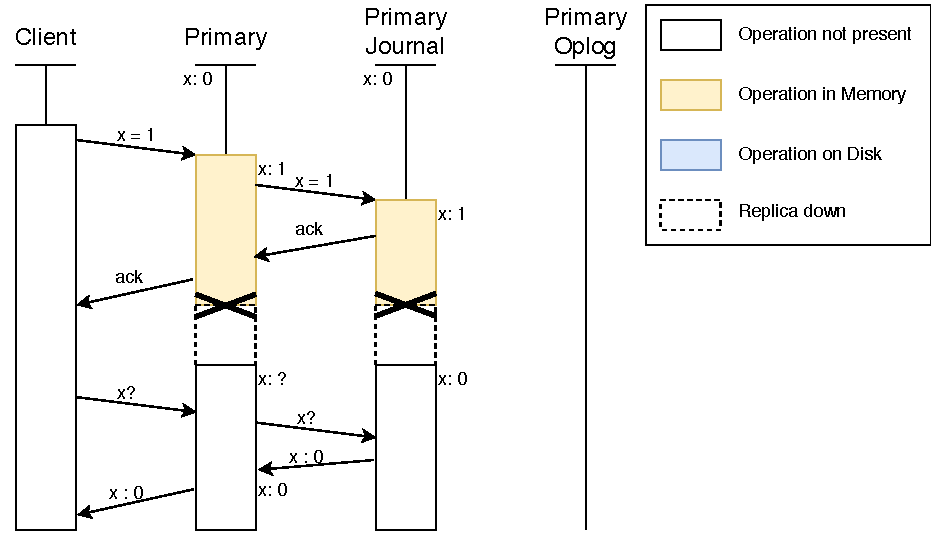
\includegraphics{images/nopersist.pdf}
    \label{fig:nopersist}
    \caption{A time-space diagram of a scenario where a write gets lost due to a failure to persist it on disk}
\end{figure}

This failure relies on two core properties of MongoDB - acknowledging a write before persisting it and only adding a write to the Oplog after flushing it to disk.

Take an operation $o$, with write concern \textit{journaled}, which has just been received by the primary. Currently, the primary stores this operation in memory, performs the operation on the in-memory copy of the data and buffers the write to the journal, but does not yet flush it to disk. Recall that a write is added to the Oplog only \textit{after} it has been flushed to disk. This creates a situation where secondary nodes do not know about a write that has been acknowledged by the primary. As such, if a primary is to crash it will "forget" about $o$ as it was only stored in memory. None of the secondary replicas would have seen $o$ either. A client querying the primary will force it to read the last value of the document operated on from disk. The value returned from the read will not account for the latest operation, which demonstrates the operation has been lost.

Thus, this failure scenario occurs with primary write concern but may also occur with journaled, if the write is buffered instead of being immediately persisted. It will not occur (in a properly implemented MongoDB system) with write concern majority.

\pagebreak
\subsection{Transient Loss via Primary Preferred Read Preference}
\begin{figure}[H]
    \centering
    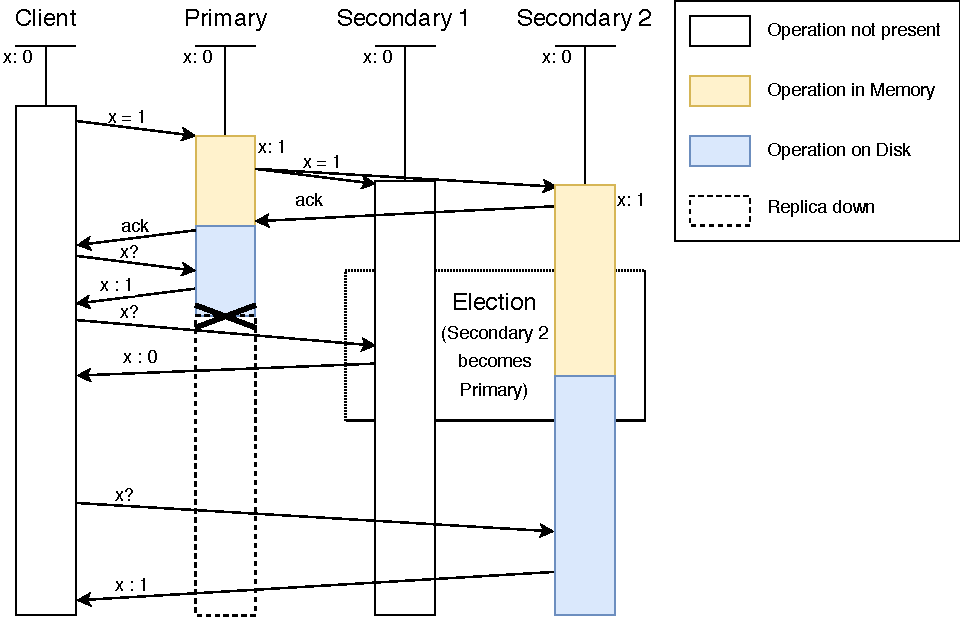
\includegraphics{images/PrimaryPreferred.pdf}
    \label{fig:primarypreferred}
    \caption{A time-space diagram of a scenario where a Majority write concern write gets temporarily lost as a result of the MongoDB client choosing the wrong Secondary to read from.}
\end{figure}

Recall from \prettyref{sec:readpref} that the Primary Preferred read preference will query the secondary if the primary appears to be down, instead of waiting for a primary to respond. The MongoDB client will only query one secondary. This can create a situation where a write will seem to be available, lost and available again. 

Specifically, consider an operation $o$ that was submitted with a majority write concern to the replica set. The primary will acknowledge the write when $\lfloor\frac{|R|}{2}\rfloor$ secondaries also acknowledge the write. This leaves $\lfloor\frac{|R|}{2}\rfloor$ secondaries that may not have acknowledged or even received the write. As such, if the primary is to fail immediately after acknowledging the operation, the MongoDB client has $\frac{\lfloor\frac{|R|}{2}\rfloor - 1}{|R|}$ chance of querying  a secondary that has not seen $o$. Intuitively, this probability reduces with time as more replicas apply the operation to their copy of the data.

If the client is to query the primary, the data returned will have operation $o$ applied to it. Once the primary fails, the MongoDB client has a chance of querying a secondary that has not applied the operation, hence the data returned from that query will not have the operation $o$ applied. Querying the new primary after an election will once again return data with operation $o$ applied. 

As such, Primary Preferred read preference can create instances of transient write loss, where acknowledged operations seem to disappear and reappear during a failure. This scenario can occur in all write concerns, but "all".
\chapter{Experiment Design \& Methodology} \label{chap:experiments}

In this chapter we offer a design and methodology of an experiment and analysis that can quantitatively evaluate the durability of a distributed storage system by measuring the frequency and quantity of write loss under failures. The experiment induces the conditions we identified in \prettyref{chap:det-theory}, and \prettyref{chap:det-results} will report on running the experiments on MongoDB.

\section{Database Contents}

Each document has a simple ID \& value structure as seen in \prettyref{alg:doc}.

\begin{algorithm}
\caption{Example document}
\begin{verbatim}
{
    Id:  5,
    Val: 7
}
\end{verbatim}
\label{alg:doc}
\end{algorithm}

\section{Methodology}

The experiment is set up by creating three identical virtual machines with the database system installed and configured to run in a replica set. We then run a stress test on the replica set using a single client on the host machine which initiates many operations, on separate threads, in parallel. The operations performed are reads, writes and updates on randomly chosen documents with randomly chosen values.

During the run of the experiment, the harness records an execution history, keeping track of each operation performed and error returned by the replica set. Each read, write and update operation is individually recorded into the execution history along with the document id corresponding to the document the operation is performed on,
the timestamp and duration of the operation. Each read record contains the value returned by the database, while the write and update records contain the new value written to the document. Any operations that result in an error are also recorded with the same data.

\begin{figure}
    \begin{CVerbatim}
R,5b9f25ef2644855182a9201c,1042661835,66.689,1537156641143
U,5b9f25ef2644855182a9201c,705768886,1.132,1537156641288
ERR,W,5b9f25f82644855182a92ff2,834995024,22.04,1537156641795
R,5b9f25ef2644855182a9201c,705768886,58.42,1537156641830
    \end{CVerbatim}
    \caption{Sample excerpt of an execution history}
\end{figure}

The experiment is broken into three stages with each stage occupying a third of the experiment time:

\begin{description}
    \item[Standard operation] The virtual machines are started in "Headless" mode and run normally.
    \item[Operating under failure] A failure is induced on the primary. The primary replica disconnects from the replica set initiating an election. 
    \item[Recovery] The failure is reverted and the failed machine is connected back to the replica set.
\end{description}

\section{Failures}

The failures induced during the experiments involve shutting down the primary replica and observing how the secondary nodes behave immediately after the shutdown. The timestamps for when a failure is induced and fixed are also entered into the execution history. 
The following failures are induced in our experiment:

\begin{description}
    \item[Graceful ACPI Shutdown] Sends an ACPI shutdown signal to the virtual machine to trigger a graceful shutdown.
    \item[Hard Poweroff] Simulates an abrupt power failure, which turns the VM off immediately.
\end{description}

Since we focus on crash-tolerant systems, we chose these failures they are supposed to be handled gracefully and correctly by the replica set. This will allow us to find concrete durability failures in the system, that should be possible to prevent within the failure assumptions the system makes. Additionally, they are common system administration scenarios of needing to restart a machine or cutting the power. The recovery flows following these failures will need to re-elect the primary after the failure and, once the failed machine is back up, allow it to "catch up" on the writes which it has not seen.

\section{Workload}
The workload of each experiment consists of three types of operations:

\begin{description}
    \item[Create Document] This operation adds a new document to the collection in the replica set. A new document is created with a value retrieved from a random number generator. Upon acknowledgement of the write from the replica set, its document ID is added to the list of IDs with acknowledged writes.
    \item[Read document] This operation queries the replica set for a document, given its key. The key for the query is chosen randomly from a list of IDs with acknowledged writes. This means, we expect that every query should return a document. Any missing documents are therefore as a result of an error in the replica set.
    \item[Update document] This operation modifies the value of an existing document. The key for the query is chosen randomly from a list of IDs with acknowledged writes and the value is generated using a random number generator.
\end{description}

The primary setting used to vary the workload of the experiment is \textit{write probability}, which determines how often a write operation is issued to the replica set. There are two types of write operations in this experiment - \textit{create document} and \textit{update document}. The decision between which operation to perform is random with equal likelihood.

In addition, we set the Read Concern, Write Concern and Read Preference. This configuration varies between experiments, allowing us to explore the tradeoffs between these configurations and understand which configuration is best for a given scenario.

\section{Execution Analysis}
The execution history produced by each run of the experiment is analysed by Algorithm \ref{alg:eval} to produce the following data:
\begin{description}
    \item[Throughput] The number of successful operations performed during the entire run of the experiment.
    \item[Errors] The number of operations that did not receive a positive acknowledgement, either they got a negative acknowledgement, or they were time out without any acknowledgement.
    \item[Lost Writes] The number of write operations which were lost either temporarily or permanently.
\end{description}

In particular, the algorithm detects when the expected value of the document and value returned from a read are not the same or where the value is missing (denoted by a value of -1). This indicates that a write has either been lost, or that it has been committed but an acknowledgement was not received by the client. We make a distinction between these two cases by keeping track of the write operations that came back as errors to the client which allows us to handle the committed-but-not-acknowledged write and update the state of our analysis as needed. 

\begin{algorithm}
    \caption{Algorithm used for evaluating the execution history}
    \begin{algorithmic}
        \STATE $H \leftarrow$ execution history
        \STATE $t_{fail} \leftarrow$ timestamp of failure induction
        \STATE $t_{fix} \leftarrow$ timestamp of failure repair
        \STATE $D \leftarrow \{\}$ \COMMENT{Lookup of every document's current value}
        \STATE $D_e \leftarrow \{\}$ \COMMENT{Lookup of every write that errored for a document}
        \STATE $E \leftarrow \{\}$ \COMMENT{Set of all errors produced}
        \STATE $M \leftarrow \{\}$ \COMMENT{Set of missing writes}
        \STATE $U \leftarrow \{\}$ \COMMENT{Set of unacknowledged writes}
        \STATE $o \leftarrow 0$ \COMMENT{Number of successful operations}
        \STATE $s \leftarrow $ Normal \COMMENT{Current state of the history (Normal, Failure or Recovery)}

        \FORALL{$h \in H$}
            \IF{$h.time \leq t_{fail}$}
                \STATE $s \leftarrow$ Normal
            \ELSIF{$t_{fail} < h.time \leq t_{fix}$}
                \STATE $s \leftarrow$ Failure
            \ELSE
                \STATE $s \leftarrow$ Recovery
            \ENDIF

            \IF{$h.op =$ Write \OR $h.op =$ Update}
                \STATE $o \leftarrow o+1$
                \STATE $D[h.id] \leftarrow h.val$
            \ELSIF{$h.op =$ Read}
                \STATE $o \leftarrow o+1$
                \IF{$h.val \neq D[h.id]$}
                    \IF{$h.id \in D_e$ \AND $h.val \in D_e[h.id]$}
                        \STATE $U \leftarrow U \cup \{(h.id, h.val, s)\}$
                        \STATE $D[h.id] \leftarrow h.val$
                        \STATE delete $h.val$ from $D_e[h.id]$
                    \ELSE
                        \STATE $M \leftarrow M \cup \{(h.id, h.val, state)\}$
                    \ENDIF
                \ENDIF
            \ELSIF{$h.op =$ Induce}
                \STATE $ s \leftarrow $ Failure
            \ELSIF{$h.op =$ Recover} 
                \STATE $ s \leftarrow $ Recovery
            \ELSIF{$h.op =$ Error}
                \STATE $E \leftarrow E \cup \{(h.err\_op, h.id, h.val, s)\}$
                \IF{$h.err\_op =$ Write \OR $h.err\_op =$ Read}
                    \STATE $D_e[h.id] \leftarrow D_e[h.id] \cup \{h.val\}$
                \ENDIF
            \ENDIF
        \ENDFOR
    \end{algorithmic}
    \label{alg:eval}
\end{algorithm}

Additionally, we also use the execution history to plot the number of different measures against the time of the experiment, bucketed using bins of 1 second.
\chapter{Results} \label{chap:kdur-results}

In this chapter, we present an empirical exploration of time-till-1-durability in MongoDB based on the theory developed in \prettyref{chap:kdur-theory} and proceed to evaluate the results in light of how MongoDB handles write operations.

\section{Environment}
The experiments were performed on the same harness as the one developed in \prettyref{chap:det-results}, using the \textit{Local} read concern and \textit{Primary} read preference. The harness was configured to \textit{not} induce a failure and perform only write operations (using write probability 1). 

\section{Estimating 1-durability}
We ran two experiments, each for 5 minutes. One with write concern \textit{w:1} and one with \textit{journaled}. The execution histories were processed to count the latencies of each operation. The raw results of this collection can be seen in \prettyref{fig:latencies}.

Given that there is a significant difference between the patterns of \textit{w:1} and \textit{journaled} histories, we use the journaled history and apply equation \prettyref{eq:persist} on every operation to derive the time a write becomes 1-durable. Given that VirtualBox networking is very stable, we subtract the average ping latency to the primary from every operation to determine the time that operation became 1-durable. A comparison between 1-durability and \textit{w:1} write acknowledgement can be found in \prettyref{fig:cdf}.

To further clarify the differences between \textit{w:1} and 1-durability, we present a chart of the difference between the two cumulative plots in \prettyref{fig:diff}.

\begin{figure}
    \centering        
    %% Creator: Matplotlib, PGF backend
%%
%% To include the figure in your LaTeX document, write
%%   \input{<filename>.pgf}
%%
%% Make sure the required packages are loaded in your preamble
%%   \usepackage{pgf}
%%
%% Figures using additional raster images can only be included by \input if
%% they are in the same directory as the main LaTeX file. For loading figures
%% from other directories you can use the `import` package
%%   \usepackage{import}
%% and then include the figures with
%%   \import{<path to file>}{<filename>.pgf}
%%
%% Matplotlib used the following preamble
%%   \usepackage[utf8x]{inputenc}
%%   \usepackage[T1]{fontenc}
%%   \usepackage{lmodern}
%%
\begingroup%
\makeatletter%
\begin{pgfpicture}%
\pgfpathrectangle{\pgfpointorigin}{\pgfqpoint{6.400000in}{4.800000in}}%
\pgfusepath{use as bounding box, clip}%
\begin{pgfscope}%
\pgfsetbuttcap%
\pgfsetmiterjoin%
\definecolor{currentfill}{rgb}{1.000000,1.000000,1.000000}%
\pgfsetfillcolor{currentfill}%
\pgfsetlinewidth{0.000000pt}%
\definecolor{currentstroke}{rgb}{1.000000,1.000000,1.000000}%
\pgfsetstrokecolor{currentstroke}%
\pgfsetdash{}{0pt}%
\pgfpathmoveto{\pgfqpoint{0.000000in}{0.000000in}}%
\pgfpathlineto{\pgfqpoint{6.400000in}{0.000000in}}%
\pgfpathlineto{\pgfqpoint{6.400000in}{4.800000in}}%
\pgfpathlineto{\pgfqpoint{0.000000in}{4.800000in}}%
\pgfpathclose%
\pgfusepath{fill}%
\end{pgfscope}%
\begin{pgfscope}%
\pgfsetbuttcap%
\pgfsetmiterjoin%
\definecolor{currentfill}{rgb}{1.000000,1.000000,1.000000}%
\pgfsetfillcolor{currentfill}%
\pgfsetlinewidth{0.000000pt}%
\definecolor{currentstroke}{rgb}{0.000000,0.000000,0.000000}%
\pgfsetstrokecolor{currentstroke}%
\pgfsetstrokeopacity{0.000000}%
\pgfsetdash{}{0pt}%
\pgfpathmoveto{\pgfqpoint{0.800000in}{0.528000in}}%
\pgfpathlineto{\pgfqpoint{5.760000in}{0.528000in}}%
\pgfpathlineto{\pgfqpoint{5.760000in}{4.224000in}}%
\pgfpathlineto{\pgfqpoint{0.800000in}{4.224000in}}%
\pgfpathclose%
\pgfusepath{fill}%
\end{pgfscope}%
\begin{pgfscope}%
\pgfsetbuttcap%
\pgfsetroundjoin%
\definecolor{currentfill}{rgb}{0.000000,0.000000,0.000000}%
\pgfsetfillcolor{currentfill}%
\pgfsetlinewidth{0.803000pt}%
\definecolor{currentstroke}{rgb}{0.000000,0.000000,0.000000}%
\pgfsetstrokecolor{currentstroke}%
\pgfsetdash{}{0pt}%
\pgfsys@defobject{currentmarker}{\pgfqpoint{0.000000in}{-0.048611in}}{\pgfqpoint{0.000000in}{0.000000in}}{%
\pgfpathmoveto{\pgfqpoint{0.000000in}{0.000000in}}%
\pgfpathlineto{\pgfqpoint{0.000000in}{-0.048611in}}%
\pgfusepath{stroke,fill}%
}%
\begin{pgfscope}%
\pgfsys@transformshift{1.020936in}{0.528000in}%
\pgfsys@useobject{currentmarker}{}%
\end{pgfscope}%
\end{pgfscope}%
\begin{pgfscope}%
\pgftext[x=1.020936in,y=0.430778in,,top]{\fontsize{11.000000}{13.200000}\selectfont \(\displaystyle 0\)}%
\end{pgfscope}%
\begin{pgfscope}%
\pgfsetbuttcap%
\pgfsetroundjoin%
\definecolor{currentfill}{rgb}{0.000000,0.000000,0.000000}%
\pgfsetfillcolor{currentfill}%
\pgfsetlinewidth{0.803000pt}%
\definecolor{currentstroke}{rgb}{0.000000,0.000000,0.000000}%
\pgfsetstrokecolor{currentstroke}%
\pgfsetdash{}{0pt}%
\pgfsys@defobject{currentmarker}{\pgfqpoint{0.000000in}{-0.048611in}}{\pgfqpoint{0.000000in}{0.000000in}}{%
\pgfpathmoveto{\pgfqpoint{0.000000in}{0.000000in}}%
\pgfpathlineto{\pgfqpoint{0.000000in}{-0.048611in}}%
\pgfusepath{stroke,fill}%
}%
\begin{pgfscope}%
\pgfsys@transformshift{1.924562in}{0.528000in}%
\pgfsys@useobject{currentmarker}{}%
\end{pgfscope}%
\end{pgfscope}%
\begin{pgfscope}%
\pgftext[x=1.924562in,y=0.430778in,,top]{\fontsize{11.000000}{13.200000}\selectfont \(\displaystyle 200\)}%
\end{pgfscope}%
\begin{pgfscope}%
\pgfsetbuttcap%
\pgfsetroundjoin%
\definecolor{currentfill}{rgb}{0.000000,0.000000,0.000000}%
\pgfsetfillcolor{currentfill}%
\pgfsetlinewidth{0.803000pt}%
\definecolor{currentstroke}{rgb}{0.000000,0.000000,0.000000}%
\pgfsetstrokecolor{currentstroke}%
\pgfsetdash{}{0pt}%
\pgfsys@defobject{currentmarker}{\pgfqpoint{0.000000in}{-0.048611in}}{\pgfqpoint{0.000000in}{0.000000in}}{%
\pgfpathmoveto{\pgfqpoint{0.000000in}{0.000000in}}%
\pgfpathlineto{\pgfqpoint{0.000000in}{-0.048611in}}%
\pgfusepath{stroke,fill}%
}%
\begin{pgfscope}%
\pgfsys@transformshift{2.828187in}{0.528000in}%
\pgfsys@useobject{currentmarker}{}%
\end{pgfscope}%
\end{pgfscope}%
\begin{pgfscope}%
\pgftext[x=2.828187in,y=0.430778in,,top]{\fontsize{11.000000}{13.200000}\selectfont \(\displaystyle 400\)}%
\end{pgfscope}%
\begin{pgfscope}%
\pgfsetbuttcap%
\pgfsetroundjoin%
\definecolor{currentfill}{rgb}{0.000000,0.000000,0.000000}%
\pgfsetfillcolor{currentfill}%
\pgfsetlinewidth{0.803000pt}%
\definecolor{currentstroke}{rgb}{0.000000,0.000000,0.000000}%
\pgfsetstrokecolor{currentstroke}%
\pgfsetdash{}{0pt}%
\pgfsys@defobject{currentmarker}{\pgfqpoint{0.000000in}{-0.048611in}}{\pgfqpoint{0.000000in}{0.000000in}}{%
\pgfpathmoveto{\pgfqpoint{0.000000in}{0.000000in}}%
\pgfpathlineto{\pgfqpoint{0.000000in}{-0.048611in}}%
\pgfusepath{stroke,fill}%
}%
\begin{pgfscope}%
\pgfsys@transformshift{3.731813in}{0.528000in}%
\pgfsys@useobject{currentmarker}{}%
\end{pgfscope}%
\end{pgfscope}%
\begin{pgfscope}%
\pgftext[x=3.731813in,y=0.430778in,,top]{\fontsize{11.000000}{13.200000}\selectfont \(\displaystyle 600\)}%
\end{pgfscope}%
\begin{pgfscope}%
\pgfsetbuttcap%
\pgfsetroundjoin%
\definecolor{currentfill}{rgb}{0.000000,0.000000,0.000000}%
\pgfsetfillcolor{currentfill}%
\pgfsetlinewidth{0.803000pt}%
\definecolor{currentstroke}{rgb}{0.000000,0.000000,0.000000}%
\pgfsetstrokecolor{currentstroke}%
\pgfsetdash{}{0pt}%
\pgfsys@defobject{currentmarker}{\pgfqpoint{0.000000in}{-0.048611in}}{\pgfqpoint{0.000000in}{0.000000in}}{%
\pgfpathmoveto{\pgfqpoint{0.000000in}{0.000000in}}%
\pgfpathlineto{\pgfqpoint{0.000000in}{-0.048611in}}%
\pgfusepath{stroke,fill}%
}%
\begin{pgfscope}%
\pgfsys@transformshift{4.635438in}{0.528000in}%
\pgfsys@useobject{currentmarker}{}%
\end{pgfscope}%
\end{pgfscope}%
\begin{pgfscope}%
\pgftext[x=4.635438in,y=0.430778in,,top]{\fontsize{11.000000}{13.200000}\selectfont \(\displaystyle 800\)}%
\end{pgfscope}%
\begin{pgfscope}%
\pgfsetbuttcap%
\pgfsetroundjoin%
\definecolor{currentfill}{rgb}{0.000000,0.000000,0.000000}%
\pgfsetfillcolor{currentfill}%
\pgfsetlinewidth{0.803000pt}%
\definecolor{currentstroke}{rgb}{0.000000,0.000000,0.000000}%
\pgfsetstrokecolor{currentstroke}%
\pgfsetdash{}{0pt}%
\pgfsys@defobject{currentmarker}{\pgfqpoint{0.000000in}{-0.048611in}}{\pgfqpoint{0.000000in}{0.000000in}}{%
\pgfpathmoveto{\pgfqpoint{0.000000in}{0.000000in}}%
\pgfpathlineto{\pgfqpoint{0.000000in}{-0.048611in}}%
\pgfusepath{stroke,fill}%
}%
\begin{pgfscope}%
\pgfsys@transformshift{5.539064in}{0.528000in}%
\pgfsys@useobject{currentmarker}{}%
\end{pgfscope}%
\end{pgfscope}%
\begin{pgfscope}%
\pgftext[x=5.539064in,y=0.430778in,,top]{\fontsize{11.000000}{13.200000}\selectfont \(\displaystyle 1000\)}%
\end{pgfscope}%
\begin{pgfscope}%
\pgftext[x=3.280000in,y=0.240271in,,top]{\fontsize{11.000000}{13.200000}\selectfont Latency (in milliseconds)}%
\end{pgfscope}%
\begin{pgfscope}%
\pgfsetbuttcap%
\pgfsetroundjoin%
\definecolor{currentfill}{rgb}{0.000000,0.000000,0.000000}%
\pgfsetfillcolor{currentfill}%
\pgfsetlinewidth{0.803000pt}%
\definecolor{currentstroke}{rgb}{0.000000,0.000000,0.000000}%
\pgfsetstrokecolor{currentstroke}%
\pgfsetdash{}{0pt}%
\pgfsys@defobject{currentmarker}{\pgfqpoint{-0.048611in}{0.000000in}}{\pgfqpoint{0.000000in}{0.000000in}}{%
\pgfpathmoveto{\pgfqpoint{0.000000in}{0.000000in}}%
\pgfpathlineto{\pgfqpoint{-0.048611in}{0.000000in}}%
\pgfusepath{stroke,fill}%
}%
\begin{pgfscope}%
\pgfsys@transformshift{0.800000in}{0.696000in}%
\pgfsys@useobject{currentmarker}{}%
\end{pgfscope}%
\end{pgfscope}%
\begin{pgfscope}%
\pgftext[x=0.627981in,y=0.643378in,left,base]{\fontsize{11.000000}{13.200000}\selectfont \(\displaystyle 0\)}%
\end{pgfscope}%
\begin{pgfscope}%
\pgfsetbuttcap%
\pgfsetroundjoin%
\definecolor{currentfill}{rgb}{0.000000,0.000000,0.000000}%
\pgfsetfillcolor{currentfill}%
\pgfsetlinewidth{0.803000pt}%
\definecolor{currentstroke}{rgb}{0.000000,0.000000,0.000000}%
\pgfsetstrokecolor{currentstroke}%
\pgfsetdash{}{0pt}%
\pgfsys@defobject{currentmarker}{\pgfqpoint{-0.048611in}{0.000000in}}{\pgfqpoint{0.000000in}{0.000000in}}{%
\pgfpathmoveto{\pgfqpoint{0.000000in}{0.000000in}}%
\pgfpathlineto{\pgfqpoint{-0.048611in}{0.000000in}}%
\pgfusepath{stroke,fill}%
}%
\begin{pgfscope}%
\pgfsys@transformshift{0.800000in}{1.129492in}%
\pgfsys@useobject{currentmarker}{}%
\end{pgfscope}%
\end{pgfscope}%
\begin{pgfscope}%
\pgftext[x=0.403588in,y=1.076870in,left,base]{\fontsize{11.000000}{13.200000}\selectfont \(\displaystyle 1000\)}%
\end{pgfscope}%
\begin{pgfscope}%
\pgfsetbuttcap%
\pgfsetroundjoin%
\definecolor{currentfill}{rgb}{0.000000,0.000000,0.000000}%
\pgfsetfillcolor{currentfill}%
\pgfsetlinewidth{0.803000pt}%
\definecolor{currentstroke}{rgb}{0.000000,0.000000,0.000000}%
\pgfsetstrokecolor{currentstroke}%
\pgfsetdash{}{0pt}%
\pgfsys@defobject{currentmarker}{\pgfqpoint{-0.048611in}{0.000000in}}{\pgfqpoint{0.000000in}{0.000000in}}{%
\pgfpathmoveto{\pgfqpoint{0.000000in}{0.000000in}}%
\pgfpathlineto{\pgfqpoint{-0.048611in}{0.000000in}}%
\pgfusepath{stroke,fill}%
}%
\begin{pgfscope}%
\pgfsys@transformshift{0.800000in}{1.562985in}%
\pgfsys@useobject{currentmarker}{}%
\end{pgfscope}%
\end{pgfscope}%
\begin{pgfscope}%
\pgftext[x=0.403588in,y=1.510363in,left,base]{\fontsize{11.000000}{13.200000}\selectfont \(\displaystyle 2000\)}%
\end{pgfscope}%
\begin{pgfscope}%
\pgfsetbuttcap%
\pgfsetroundjoin%
\definecolor{currentfill}{rgb}{0.000000,0.000000,0.000000}%
\pgfsetfillcolor{currentfill}%
\pgfsetlinewidth{0.803000pt}%
\definecolor{currentstroke}{rgb}{0.000000,0.000000,0.000000}%
\pgfsetstrokecolor{currentstroke}%
\pgfsetdash{}{0pt}%
\pgfsys@defobject{currentmarker}{\pgfqpoint{-0.048611in}{0.000000in}}{\pgfqpoint{0.000000in}{0.000000in}}{%
\pgfpathmoveto{\pgfqpoint{0.000000in}{0.000000in}}%
\pgfpathlineto{\pgfqpoint{-0.048611in}{0.000000in}}%
\pgfusepath{stroke,fill}%
}%
\begin{pgfscope}%
\pgfsys@transformshift{0.800000in}{1.996477in}%
\pgfsys@useobject{currentmarker}{}%
\end{pgfscope}%
\end{pgfscope}%
\begin{pgfscope}%
\pgftext[x=0.403588in,y=1.943855in,left,base]{\fontsize{11.000000}{13.200000}\selectfont \(\displaystyle 3000\)}%
\end{pgfscope}%
\begin{pgfscope}%
\pgfsetbuttcap%
\pgfsetroundjoin%
\definecolor{currentfill}{rgb}{0.000000,0.000000,0.000000}%
\pgfsetfillcolor{currentfill}%
\pgfsetlinewidth{0.803000pt}%
\definecolor{currentstroke}{rgb}{0.000000,0.000000,0.000000}%
\pgfsetstrokecolor{currentstroke}%
\pgfsetdash{}{0pt}%
\pgfsys@defobject{currentmarker}{\pgfqpoint{-0.048611in}{0.000000in}}{\pgfqpoint{0.000000in}{0.000000in}}{%
\pgfpathmoveto{\pgfqpoint{0.000000in}{0.000000in}}%
\pgfpathlineto{\pgfqpoint{-0.048611in}{0.000000in}}%
\pgfusepath{stroke,fill}%
}%
\begin{pgfscope}%
\pgfsys@transformshift{0.800000in}{2.429970in}%
\pgfsys@useobject{currentmarker}{}%
\end{pgfscope}%
\end{pgfscope}%
\begin{pgfscope}%
\pgftext[x=0.403588in,y=2.377348in,left,base]{\fontsize{11.000000}{13.200000}\selectfont \(\displaystyle 4000\)}%
\end{pgfscope}%
\begin{pgfscope}%
\pgfsetbuttcap%
\pgfsetroundjoin%
\definecolor{currentfill}{rgb}{0.000000,0.000000,0.000000}%
\pgfsetfillcolor{currentfill}%
\pgfsetlinewidth{0.803000pt}%
\definecolor{currentstroke}{rgb}{0.000000,0.000000,0.000000}%
\pgfsetstrokecolor{currentstroke}%
\pgfsetdash{}{0pt}%
\pgfsys@defobject{currentmarker}{\pgfqpoint{-0.048611in}{0.000000in}}{\pgfqpoint{0.000000in}{0.000000in}}{%
\pgfpathmoveto{\pgfqpoint{0.000000in}{0.000000in}}%
\pgfpathlineto{\pgfqpoint{-0.048611in}{0.000000in}}%
\pgfusepath{stroke,fill}%
}%
\begin{pgfscope}%
\pgfsys@transformshift{0.800000in}{2.863462in}%
\pgfsys@useobject{currentmarker}{}%
\end{pgfscope}%
\end{pgfscope}%
\begin{pgfscope}%
\pgftext[x=0.403588in,y=2.810840in,left,base]{\fontsize{11.000000}{13.200000}\selectfont \(\displaystyle 5000\)}%
\end{pgfscope}%
\begin{pgfscope}%
\pgfsetbuttcap%
\pgfsetroundjoin%
\definecolor{currentfill}{rgb}{0.000000,0.000000,0.000000}%
\pgfsetfillcolor{currentfill}%
\pgfsetlinewidth{0.803000pt}%
\definecolor{currentstroke}{rgb}{0.000000,0.000000,0.000000}%
\pgfsetstrokecolor{currentstroke}%
\pgfsetdash{}{0pt}%
\pgfsys@defobject{currentmarker}{\pgfqpoint{-0.048611in}{0.000000in}}{\pgfqpoint{0.000000in}{0.000000in}}{%
\pgfpathmoveto{\pgfqpoint{0.000000in}{0.000000in}}%
\pgfpathlineto{\pgfqpoint{-0.048611in}{0.000000in}}%
\pgfusepath{stroke,fill}%
}%
\begin{pgfscope}%
\pgfsys@transformshift{0.800000in}{3.296955in}%
\pgfsys@useobject{currentmarker}{}%
\end{pgfscope}%
\end{pgfscope}%
\begin{pgfscope}%
\pgftext[x=0.403588in,y=3.244332in,left,base]{\fontsize{11.000000}{13.200000}\selectfont \(\displaystyle 6000\)}%
\end{pgfscope}%
\begin{pgfscope}%
\pgfsetbuttcap%
\pgfsetroundjoin%
\definecolor{currentfill}{rgb}{0.000000,0.000000,0.000000}%
\pgfsetfillcolor{currentfill}%
\pgfsetlinewidth{0.803000pt}%
\definecolor{currentstroke}{rgb}{0.000000,0.000000,0.000000}%
\pgfsetstrokecolor{currentstroke}%
\pgfsetdash{}{0pt}%
\pgfsys@defobject{currentmarker}{\pgfqpoint{-0.048611in}{0.000000in}}{\pgfqpoint{0.000000in}{0.000000in}}{%
\pgfpathmoveto{\pgfqpoint{0.000000in}{0.000000in}}%
\pgfpathlineto{\pgfqpoint{-0.048611in}{0.000000in}}%
\pgfusepath{stroke,fill}%
}%
\begin{pgfscope}%
\pgfsys@transformshift{0.800000in}{3.730447in}%
\pgfsys@useobject{currentmarker}{}%
\end{pgfscope}%
\end{pgfscope}%
\begin{pgfscope}%
\pgftext[x=0.403588in,y=3.677825in,left,base]{\fontsize{11.000000}{13.200000}\selectfont \(\displaystyle 7000\)}%
\end{pgfscope}%
\begin{pgfscope}%
\pgfsetbuttcap%
\pgfsetroundjoin%
\definecolor{currentfill}{rgb}{0.000000,0.000000,0.000000}%
\pgfsetfillcolor{currentfill}%
\pgfsetlinewidth{0.803000pt}%
\definecolor{currentstroke}{rgb}{0.000000,0.000000,0.000000}%
\pgfsetstrokecolor{currentstroke}%
\pgfsetdash{}{0pt}%
\pgfsys@defobject{currentmarker}{\pgfqpoint{-0.048611in}{0.000000in}}{\pgfqpoint{0.000000in}{0.000000in}}{%
\pgfpathmoveto{\pgfqpoint{0.000000in}{0.000000in}}%
\pgfpathlineto{\pgfqpoint{-0.048611in}{0.000000in}}%
\pgfusepath{stroke,fill}%
}%
\begin{pgfscope}%
\pgfsys@transformshift{0.800000in}{4.163940in}%
\pgfsys@useobject{currentmarker}{}%
\end{pgfscope}%
\end{pgfscope}%
\begin{pgfscope}%
\pgftext[x=0.403588in,y=4.111317in,left,base]{\fontsize{11.000000}{13.200000}\selectfont \(\displaystyle 8000\)}%
\end{pgfscope}%
\begin{pgfscope}%
\pgftext[x=0.348033in,y=2.376000in,,bottom,rotate=90.000000]{\fontsize{11.000000}{13.200000}\selectfont Number of operations}%
\end{pgfscope}%
\begin{pgfscope}%
\pgfpathrectangle{\pgfqpoint{0.800000in}{0.528000in}}{\pgfqpoint{4.960000in}{3.696000in}}%
\pgfusepath{clip}%
\pgfsetrectcap%
\pgfsetroundjoin%
\pgfsetlinewidth{1.505625pt}%
\definecolor{currentstroke}{rgb}{0.121569,0.466667,0.705882}%
\pgfsetstrokecolor{currentstroke}%
\pgfsetdash{}{0pt}%
\pgfpathmoveto{\pgfqpoint{1.025455in}{1.752855in}}%
\pgfpathlineto{\pgfqpoint{1.029973in}{1.641447in}}%
\pgfpathlineto{\pgfqpoint{1.034491in}{1.632344in}}%
\pgfpathlineto{\pgfqpoint{1.039009in}{1.615871in}}%
\pgfpathlineto{\pgfqpoint{1.043527in}{1.570788in}}%
\pgfpathlineto{\pgfqpoint{1.048045in}{1.623674in}}%
\pgfpathlineto{\pgfqpoint{1.052563in}{1.613270in}}%
\pgfpathlineto{\pgfqpoint{1.061600in}{1.502296in}}%
\pgfpathlineto{\pgfqpoint{1.066118in}{1.454178in}}%
\pgfpathlineto{\pgfqpoint{1.070636in}{1.436839in}}%
\pgfpathlineto{\pgfqpoint{1.075154in}{1.357943in}}%
\pgfpathlineto{\pgfqpoint{1.079672in}{1.379184in}}%
\pgfpathlineto{\pgfqpoint{1.084190in}{1.332367in}}%
\pgfpathlineto{\pgfqpoint{1.097745in}{1.240467in}}%
\pgfpathlineto{\pgfqpoint{1.102263in}{1.184979in}}%
\pgfpathlineto{\pgfqpoint{1.106781in}{1.148133in}}%
\pgfpathlineto{\pgfqpoint{1.111299in}{1.142064in}}%
\pgfpathlineto{\pgfqpoint{1.115817in}{1.080941in}}%
\pgfpathlineto{\pgfqpoint{1.120335in}{1.077473in}}%
\pgfpathlineto{\pgfqpoint{1.124853in}{1.051897in}}%
\pgfpathlineto{\pgfqpoint{1.129371in}{1.044961in}}%
\pgfpathlineto{\pgfqpoint{1.133890in}{1.019819in}}%
\pgfpathlineto{\pgfqpoint{1.138408in}{1.002479in}}%
\pgfpathlineto{\pgfqpoint{1.147444in}{0.945692in}}%
\pgfpathlineto{\pgfqpoint{1.151962in}{0.924451in}}%
\pgfpathlineto{\pgfqpoint{1.156480in}{0.941790in}}%
\pgfpathlineto{\pgfqpoint{1.160998in}{0.890638in}}%
\pgfpathlineto{\pgfqpoint{1.165516in}{0.902342in}}%
\pgfpathlineto{\pgfqpoint{1.174553in}{0.842087in}}%
\pgfpathlineto{\pgfqpoint{1.179071in}{0.838186in}}%
\pgfpathlineto{\pgfqpoint{1.183589in}{0.841220in}}%
\pgfpathlineto{\pgfqpoint{1.188107in}{0.829082in}}%
\pgfpathlineto{\pgfqpoint{1.192625in}{0.837752in}}%
\pgfpathlineto{\pgfqpoint{1.197143in}{0.825181in}}%
\pgfpathlineto{\pgfqpoint{1.201662in}{0.835151in}}%
\pgfpathlineto{\pgfqpoint{1.206180in}{0.827782in}}%
\pgfpathlineto{\pgfqpoint{1.210698in}{0.845988in}}%
\pgfpathlineto{\pgfqpoint{1.215216in}{0.857693in}}%
\pgfpathlineto{\pgfqpoint{1.219734in}{0.886303in}}%
\pgfpathlineto{\pgfqpoint{1.224252in}{0.924451in}}%
\pgfpathlineto{\pgfqpoint{1.228770in}{0.944825in}}%
\pgfpathlineto{\pgfqpoint{1.237807in}{1.063602in}}%
\pgfpathlineto{\pgfqpoint{1.242325in}{1.126025in}}%
\pgfpathlineto{\pgfqpoint{1.246843in}{1.347973in}}%
\pgfpathlineto{\pgfqpoint{1.251361in}{1.315461in}}%
\pgfpathlineto{\pgfqpoint{1.255879in}{1.435105in}}%
\pgfpathlineto{\pgfqpoint{1.260397in}{1.496661in}}%
\pgfpathlineto{\pgfqpoint{1.264915in}{1.742884in}}%
\pgfpathlineto{\pgfqpoint{1.273952in}{2.383153in}}%
\pgfpathlineto{\pgfqpoint{1.278470in}{2.811877in}}%
\pgfpathlineto{\pgfqpoint{1.282988in}{2.925018in}}%
\pgfpathlineto{\pgfqpoint{1.287506in}{2.944959in}}%
\pgfpathlineto{\pgfqpoint{1.292024in}{3.285684in}}%
\pgfpathlineto{\pgfqpoint{1.296542in}{3.500696in}}%
\pgfpathlineto{\pgfqpoint{1.301060in}{3.795471in}}%
\pgfpathlineto{\pgfqpoint{1.305578in}{3.819747in}}%
\pgfpathlineto{\pgfqpoint{1.310097in}{3.826249in}}%
\pgfpathlineto{\pgfqpoint{1.314615in}{4.056000in}}%
\pgfpathlineto{\pgfqpoint{1.319133in}{3.809343in}}%
\pgfpathlineto{\pgfqpoint{1.323651in}{3.720477in}}%
\pgfpathlineto{\pgfqpoint{1.328169in}{3.785934in}}%
\pgfpathlineto{\pgfqpoint{1.332687in}{3.953262in}}%
\pgfpathlineto{\pgfqpoint{1.337205in}{4.017853in}}%
\pgfpathlineto{\pgfqpoint{1.341723in}{4.033458in}}%
\pgfpathlineto{\pgfqpoint{1.346242in}{3.977104in}}%
\pgfpathlineto{\pgfqpoint{1.355278in}{3.625975in}}%
\pgfpathlineto{\pgfqpoint{1.359796in}{3.322097in}}%
\pgfpathlineto{\pgfqpoint{1.364314in}{3.151735in}}%
\pgfpathlineto{\pgfqpoint{1.368832in}{2.882969in}}%
\pgfpathlineto{\pgfqpoint{1.391423in}{2.148200in}}%
\pgfpathlineto{\pgfqpoint{1.400459in}{1.983906in}}%
\pgfpathlineto{\pgfqpoint{1.404977in}{1.849957in}}%
\pgfpathlineto{\pgfqpoint{1.414013in}{1.676993in}}%
\pgfpathlineto{\pgfqpoint{1.423050in}{1.565152in}}%
\pgfpathlineto{\pgfqpoint{1.427568in}{1.466316in}}%
\pgfpathlineto{\pgfqpoint{1.432086in}{1.421666in}}%
\pgfpathlineto{\pgfqpoint{1.436604in}{1.327599in}}%
\pgfpathlineto{\pgfqpoint{1.441122in}{1.269077in}}%
\pgfpathlineto{\pgfqpoint{1.445640in}{1.277747in}}%
\pgfpathlineto{\pgfqpoint{1.450158in}{1.276013in}}%
\pgfpathlineto{\pgfqpoint{1.454677in}{1.243067in}}%
\pgfpathlineto{\pgfqpoint{1.459195in}{1.229629in}}%
\pgfpathlineto{\pgfqpoint{1.463713in}{1.184979in}}%
\pgfpathlineto{\pgfqpoint{1.468231in}{1.108251in}}%
\pgfpathlineto{\pgfqpoint{1.472749in}{1.091345in}}%
\pgfpathlineto{\pgfqpoint{1.477267in}{1.093513in}}%
\pgfpathlineto{\pgfqpoint{1.481785in}{1.081375in}}%
\pgfpathlineto{\pgfqpoint{1.490822in}{0.973435in}}%
\pgfpathlineto{\pgfqpoint{1.495340in}{0.980371in}}%
\pgfpathlineto{\pgfqpoint{1.499858in}{1.012016in}}%
\pgfpathlineto{\pgfqpoint{1.504376in}{0.963898in}}%
\pgfpathlineto{\pgfqpoint{1.508894in}{0.977337in}}%
\pgfpathlineto{\pgfqpoint{1.513412in}{1.004647in}}%
\pgfpathlineto{\pgfqpoint{1.517930in}{1.020252in}}%
\pgfpathlineto{\pgfqpoint{1.522449in}{1.025454in}}%
\pgfpathlineto{\pgfqpoint{1.526967in}{1.078774in}}%
\pgfpathlineto{\pgfqpoint{1.531485in}{1.110852in}}%
\pgfpathlineto{\pgfqpoint{1.536003in}{1.189748in}}%
\pgfpathlineto{\pgfqpoint{1.540521in}{1.138162in}}%
\pgfpathlineto{\pgfqpoint{1.545039in}{1.237432in}}%
\pgfpathlineto{\pgfqpoint{1.554075in}{1.305057in}}%
\pgfpathlineto{\pgfqpoint{1.558594in}{1.378317in}}%
\pgfpathlineto{\pgfqpoint{1.563112in}{1.471951in}}%
\pgfpathlineto{\pgfqpoint{1.567630in}{1.603300in}}%
\pgfpathlineto{\pgfqpoint{1.572148in}{1.550847in}}%
\pgfpathlineto{\pgfqpoint{1.576666in}{1.672658in}}%
\pgfpathlineto{\pgfqpoint{1.581184in}{1.702136in}}%
\pgfpathlineto{\pgfqpoint{1.585702in}{1.791435in}}%
\pgfpathlineto{\pgfqpoint{1.590220in}{1.761091in}}%
\pgfpathlineto{\pgfqpoint{1.599257in}{1.924084in}}%
\pgfpathlineto{\pgfqpoint{1.612811in}{2.146899in}}%
\pgfpathlineto{\pgfqpoint{1.617329in}{2.258307in}}%
\pgfpathlineto{\pgfqpoint{1.621847in}{2.423467in}}%
\pgfpathlineto{\pgfqpoint{1.626365in}{2.496294in}}%
\pgfpathlineto{\pgfqpoint{1.630884in}{2.638480in}}%
\pgfpathlineto{\pgfqpoint{1.635402in}{2.709572in}}%
\pgfpathlineto{\pgfqpoint{1.639920in}{2.857827in}}%
\pgfpathlineto{\pgfqpoint{1.644438in}{2.914181in}}%
\pgfpathlineto{\pgfqpoint{1.648956in}{3.095814in}}%
\pgfpathlineto{\pgfqpoint{1.653474in}{2.964033in}}%
\pgfpathlineto{\pgfqpoint{1.657992in}{3.016485in}}%
\pgfpathlineto{\pgfqpoint{1.662510in}{3.015185in}}%
\pgfpathlineto{\pgfqpoint{1.667029in}{2.932821in}}%
\pgfpathlineto{\pgfqpoint{1.671547in}{2.747286in}}%
\pgfpathlineto{\pgfqpoint{1.676065in}{2.692233in}}%
\pgfpathlineto{\pgfqpoint{1.685101in}{2.489792in}}%
\pgfpathlineto{\pgfqpoint{1.689619in}{2.528373in}}%
\pgfpathlineto{\pgfqpoint{1.694137in}{2.403527in}}%
\pgfpathlineto{\pgfqpoint{1.698655in}{2.352808in}}%
\pgfpathlineto{\pgfqpoint{1.703174in}{2.323764in}}%
\pgfpathlineto{\pgfqpoint{1.707692in}{2.322464in}}%
\pgfpathlineto{\pgfqpoint{1.716728in}{2.035925in}}%
\pgfpathlineto{\pgfqpoint{1.721246in}{2.004280in}}%
\pgfpathlineto{\pgfqpoint{1.725764in}{1.848656in}}%
\pgfpathlineto{\pgfqpoint{1.730282in}{1.737249in}}%
\pgfpathlineto{\pgfqpoint{1.734801in}{1.731180in}}%
\pgfpathlineto{\pgfqpoint{1.739319in}{1.646215in}}%
\pgfpathlineto{\pgfqpoint{1.748355in}{1.534808in}}%
\pgfpathlineto{\pgfqpoint{1.752873in}{1.513133in}}%
\pgfpathlineto{\pgfqpoint{1.757391in}{1.441607in}}%
\pgfpathlineto{\pgfqpoint{1.766427in}{1.376583in}}%
\pgfpathlineto{\pgfqpoint{1.770946in}{1.371815in}}%
\pgfpathlineto{\pgfqpoint{1.775464in}{1.348406in}}%
\pgfpathlineto{\pgfqpoint{1.779982in}{1.292919in}}%
\pgfpathlineto{\pgfqpoint{1.784500in}{1.255205in}}%
\pgfpathlineto{\pgfqpoint{1.789018in}{1.234831in}}%
\pgfpathlineto{\pgfqpoint{1.793536in}{1.250870in}}%
\pgfpathlineto{\pgfqpoint{1.798054in}{1.214890in}}%
\pgfpathlineto{\pgfqpoint{1.802572in}{1.282949in}}%
\pgfpathlineto{\pgfqpoint{1.807091in}{1.157669in}}%
\pgfpathlineto{\pgfqpoint{1.811609in}{1.167206in}}%
\pgfpathlineto{\pgfqpoint{1.820645in}{1.200585in}}%
\pgfpathlineto{\pgfqpoint{1.825163in}{1.212290in}}%
\pgfpathlineto{\pgfqpoint{1.829681in}{1.228762in}}%
\pgfpathlineto{\pgfqpoint{1.834199in}{1.258240in}}%
\pgfpathlineto{\pgfqpoint{1.838717in}{1.209689in}}%
\pgfpathlineto{\pgfqpoint{1.843236in}{1.213156in}}%
\pgfpathlineto{\pgfqpoint{1.847754in}{1.293353in}}%
\pgfpathlineto{\pgfqpoint{1.852272in}{1.214890in}}%
\pgfpathlineto{\pgfqpoint{1.856790in}{1.219225in}}%
\pgfpathlineto{\pgfqpoint{1.861308in}{1.263008in}}%
\pgfpathlineto{\pgfqpoint{1.865826in}{1.239166in}}%
\pgfpathlineto{\pgfqpoint{1.870344in}{1.230063in}}%
\pgfpathlineto{\pgfqpoint{1.874862in}{1.254338in}}%
\pgfpathlineto{\pgfqpoint{1.879381in}{1.372248in}}%
\pgfpathlineto{\pgfqpoint{1.883899in}{1.419499in}}%
\pgfpathlineto{\pgfqpoint{1.888417in}{1.355342in}}%
\pgfpathlineto{\pgfqpoint{1.892935in}{1.405194in}}%
\pgfpathlineto{\pgfqpoint{1.897453in}{1.474552in}}%
\pgfpathlineto{\pgfqpoint{1.901971in}{1.505764in}}%
\pgfpathlineto{\pgfqpoint{1.906489in}{1.510532in}}%
\pgfpathlineto{\pgfqpoint{1.911007in}{1.559950in}}%
\pgfpathlineto{\pgfqpoint{1.915526in}{1.534808in}}%
\pgfpathlineto{\pgfqpoint{1.920044in}{1.527005in}}%
\pgfpathlineto{\pgfqpoint{1.924562in}{1.527872in}}%
\pgfpathlineto{\pgfqpoint{1.929080in}{1.539576in}}%
\pgfpathlineto{\pgfqpoint{1.933598in}{1.578157in}}%
\pgfpathlineto{\pgfqpoint{1.938116in}{1.629743in}}%
\pgfpathlineto{\pgfqpoint{1.942634in}{1.619339in}}%
\pgfpathlineto{\pgfqpoint{1.947152in}{1.644915in}}%
\pgfpathlineto{\pgfqpoint{1.951671in}{1.618905in}}%
\pgfpathlineto{\pgfqpoint{1.956189in}{1.713840in}}%
\pgfpathlineto{\pgfqpoint{1.960707in}{1.715574in}}%
\pgfpathlineto{\pgfqpoint{1.965225in}{1.683929in}}%
\pgfpathlineto{\pgfqpoint{1.969743in}{1.739416in}}%
\pgfpathlineto{\pgfqpoint{1.974261in}{1.658353in}}%
\pgfpathlineto{\pgfqpoint{1.978779in}{1.670925in}}%
\pgfpathlineto{\pgfqpoint{1.983298in}{1.674392in}}%
\pgfpathlineto{\pgfqpoint{1.987816in}{1.630176in}}%
\pgfpathlineto{\pgfqpoint{1.992334in}{1.604600in}}%
\pgfpathlineto{\pgfqpoint{1.996852in}{1.597664in}}%
\pgfpathlineto{\pgfqpoint{2.001370in}{1.546512in}}%
\pgfpathlineto{\pgfqpoint{2.005888in}{1.535675in}}%
\pgfpathlineto{\pgfqpoint{2.010406in}{1.495794in}}%
\pgfpathlineto{\pgfqpoint{2.014924in}{1.471085in}}%
\pgfpathlineto{\pgfqpoint{2.019443in}{1.459814in}}%
\pgfpathlineto{\pgfqpoint{2.023961in}{1.429469in}}%
\pgfpathlineto{\pgfqpoint{2.028479in}{1.416031in}}%
\pgfpathlineto{\pgfqpoint{2.032997in}{1.307224in}}%
\pgfpathlineto{\pgfqpoint{2.037515in}{1.298121in}}%
\pgfpathlineto{\pgfqpoint{2.042033in}{1.270811in}}%
\pgfpathlineto{\pgfqpoint{2.046551in}{1.305057in}}%
\pgfpathlineto{\pgfqpoint{2.055588in}{1.193216in}}%
\pgfpathlineto{\pgfqpoint{2.060106in}{1.197551in}}%
\pgfpathlineto{\pgfqpoint{2.064624in}{1.167640in}}%
\pgfpathlineto{\pgfqpoint{2.069142in}{1.180211in}}%
\pgfpathlineto{\pgfqpoint{2.078178in}{1.181078in}}%
\pgfpathlineto{\pgfqpoint{2.082696in}{1.118222in}}%
\pgfpathlineto{\pgfqpoint{2.087214in}{1.116921in}}%
\pgfpathlineto{\pgfqpoint{2.096251in}{1.060567in}}%
\pgfpathlineto{\pgfqpoint{2.100769in}{1.091345in}}%
\pgfpathlineto{\pgfqpoint{2.105287in}{1.045828in}}%
\pgfpathlineto{\pgfqpoint{2.109805in}{1.063168in}}%
\pgfpathlineto{\pgfqpoint{2.118841in}{1.065769in}}%
\pgfpathlineto{\pgfqpoint{2.123359in}{1.065769in}}%
\pgfpathlineto{\pgfqpoint{2.127878in}{1.069670in}}%
\pgfpathlineto{\pgfqpoint{2.132396in}{1.080508in}}%
\pgfpathlineto{\pgfqpoint{2.136914in}{1.110852in}}%
\pgfpathlineto{\pgfqpoint{2.141432in}{1.132527in}}%
\pgfpathlineto{\pgfqpoint{2.145950in}{1.087877in}}%
\pgfpathlineto{\pgfqpoint{2.150468in}{1.098281in}}%
\pgfpathlineto{\pgfqpoint{2.154986in}{1.043661in}}%
\pgfpathlineto{\pgfqpoint{2.159504in}{1.046262in}}%
\pgfpathlineto{\pgfqpoint{2.164023in}{1.050597in}}%
\pgfpathlineto{\pgfqpoint{2.168541in}{1.042360in}}%
\pgfpathlineto{\pgfqpoint{2.173059in}{1.054065in}}%
\pgfpathlineto{\pgfqpoint{2.177577in}{1.044094in}}%
\pgfpathlineto{\pgfqpoint{2.182095in}{1.062735in}}%
\pgfpathlineto{\pgfqpoint{2.186613in}{1.045828in}}%
\pgfpathlineto{\pgfqpoint{2.191131in}{1.065336in}}%
\pgfpathlineto{\pgfqpoint{2.195649in}{1.025888in}}%
\pgfpathlineto{\pgfqpoint{2.200168in}{1.018518in}}%
\pgfpathlineto{\pgfqpoint{2.209204in}{1.017651in}}%
\pgfpathlineto{\pgfqpoint{2.213722in}{1.010282in}}%
\pgfpathlineto{\pgfqpoint{2.218240in}{0.992509in}}%
\pgfpathlineto{\pgfqpoint{2.222758in}{1.012449in}}%
\pgfpathlineto{\pgfqpoint{2.227276in}{1.044528in}}%
\pgfpathlineto{\pgfqpoint{2.231794in}{1.058833in}}%
\pgfpathlineto{\pgfqpoint{2.236313in}{1.053631in}}%
\pgfpathlineto{\pgfqpoint{2.240831in}{1.053631in}}%
\pgfpathlineto{\pgfqpoint{2.245349in}{1.078340in}}%
\pgfpathlineto{\pgfqpoint{2.249867in}{1.061868in}}%
\pgfpathlineto{\pgfqpoint{2.254385in}{1.104783in}}%
\pgfpathlineto{\pgfqpoint{2.258903in}{1.101315in}}%
\pgfpathlineto{\pgfqpoint{2.263421in}{1.121256in}}%
\pgfpathlineto{\pgfqpoint{2.267940in}{1.091345in}}%
\pgfpathlineto{\pgfqpoint{2.272458in}{1.104350in}}%
\pgfpathlineto{\pgfqpoint{2.276976in}{1.075739in}}%
\pgfpathlineto{\pgfqpoint{2.281494in}{1.073138in}}%
\pgfpathlineto{\pgfqpoint{2.286012in}{1.079641in}}%
\pgfpathlineto{\pgfqpoint{2.290530in}{1.070537in}}%
\pgfpathlineto{\pgfqpoint{2.295048in}{1.037592in}}%
\pgfpathlineto{\pgfqpoint{2.299566in}{1.016351in}}%
\pgfpathlineto{\pgfqpoint{2.304085in}{1.087010in}}%
\pgfpathlineto{\pgfqpoint{2.308603in}{1.055799in}}%
\pgfpathlineto{\pgfqpoint{2.313121in}{1.049296in}}%
\pgfpathlineto{\pgfqpoint{2.317639in}{1.044961in}}%
\pgfpathlineto{\pgfqpoint{2.322157in}{1.050597in}}%
\pgfpathlineto{\pgfqpoint{2.331193in}{0.992509in}}%
\pgfpathlineto{\pgfqpoint{2.335711in}{0.999445in}}%
\pgfpathlineto{\pgfqpoint{2.340230in}{0.978637in}}%
\pgfpathlineto{\pgfqpoint{2.344748in}{0.994676in}}%
\pgfpathlineto{\pgfqpoint{2.353784in}{0.953928in}}%
\pgfpathlineto{\pgfqpoint{2.358302in}{0.948293in}}%
\pgfpathlineto{\pgfqpoint{2.362820in}{1.014617in}}%
\pgfpathlineto{\pgfqpoint{2.367338in}{0.963031in}}%
\pgfpathlineto{\pgfqpoint{2.371856in}{0.946559in}}%
\pgfpathlineto{\pgfqpoint{2.376375in}{0.925751in}}%
\pgfpathlineto{\pgfqpoint{2.380893in}{0.924884in}}%
\pgfpathlineto{\pgfqpoint{2.389929in}{0.917081in}}%
\pgfpathlineto{\pgfqpoint{2.394447in}{0.940923in}}%
\pgfpathlineto{\pgfqpoint{2.398965in}{0.937022in}}%
\pgfpathlineto{\pgfqpoint{2.403483in}{0.937889in}}%
\pgfpathlineto{\pgfqpoint{2.408001in}{0.903209in}}%
\pgfpathlineto{\pgfqpoint{2.412520in}{0.904943in}}%
\pgfpathlineto{\pgfqpoint{2.417038in}{0.909278in}}%
\pgfpathlineto{\pgfqpoint{2.421556in}{0.923150in}}%
\pgfpathlineto{\pgfqpoint{2.426074in}{0.915781in}}%
\pgfpathlineto{\pgfqpoint{2.430592in}{0.949593in}}%
\pgfpathlineto{\pgfqpoint{2.439628in}{0.933987in}}%
\pgfpathlineto{\pgfqpoint{2.444146in}{0.941357in}}%
\pgfpathlineto{\pgfqpoint{2.448665in}{0.920116in}}%
\pgfpathlineto{\pgfqpoint{2.453183in}{0.887604in}}%
\pgfpathlineto{\pgfqpoint{2.457701in}{0.885003in}}%
\pgfpathlineto{\pgfqpoint{2.466737in}{0.915347in}}%
\pgfpathlineto{\pgfqpoint{2.471255in}{0.906677in}}%
\pgfpathlineto{\pgfqpoint{2.475773in}{0.875899in}}%
\pgfpathlineto{\pgfqpoint{2.484810in}{0.877633in}}%
\pgfpathlineto{\pgfqpoint{2.493846in}{0.866363in}}%
\pgfpathlineto{\pgfqpoint{2.498364in}{0.878934in}}%
\pgfpathlineto{\pgfqpoint{2.502882in}{0.871564in}}%
\pgfpathlineto{\pgfqpoint{2.507400in}{0.881101in}}%
\pgfpathlineto{\pgfqpoint{2.511918in}{0.867230in}}%
\pgfpathlineto{\pgfqpoint{2.516437in}{0.889771in}}%
\pgfpathlineto{\pgfqpoint{2.520955in}{0.878934in}}%
\pgfpathlineto{\pgfqpoint{2.525473in}{0.881535in}}%
\pgfpathlineto{\pgfqpoint{2.529991in}{0.880668in}}%
\pgfpathlineto{\pgfqpoint{2.534509in}{0.864629in}}%
\pgfpathlineto{\pgfqpoint{2.539027in}{0.874599in}}%
\pgfpathlineto{\pgfqpoint{2.543545in}{0.860727in}}%
\pgfpathlineto{\pgfqpoint{2.548063in}{0.868963in}}%
\pgfpathlineto{\pgfqpoint{2.552582in}{0.857259in}}%
\pgfpathlineto{\pgfqpoint{2.557100in}{0.876333in}}%
\pgfpathlineto{\pgfqpoint{2.561618in}{0.872865in}}%
\pgfpathlineto{\pgfqpoint{2.566136in}{0.862028in}}%
\pgfpathlineto{\pgfqpoint{2.575172in}{0.876333in}}%
\pgfpathlineto{\pgfqpoint{2.579690in}{0.878500in}}%
\pgfpathlineto{\pgfqpoint{2.584208in}{0.876766in}}%
\pgfpathlineto{\pgfqpoint{2.588727in}{0.857259in}}%
\pgfpathlineto{\pgfqpoint{2.593245in}{0.849890in}}%
\pgfpathlineto{\pgfqpoint{2.597763in}{0.853791in}}%
\pgfpathlineto{\pgfqpoint{2.602281in}{0.869830in}}%
\pgfpathlineto{\pgfqpoint{2.611317in}{0.865496in}}%
\pgfpathlineto{\pgfqpoint{2.615835in}{0.868963in}}%
\pgfpathlineto{\pgfqpoint{2.620353in}{0.856392in}}%
\pgfpathlineto{\pgfqpoint{2.624872in}{0.862028in}}%
\pgfpathlineto{\pgfqpoint{2.629390in}{0.849023in}}%
\pgfpathlineto{\pgfqpoint{2.633908in}{0.866363in}}%
\pgfpathlineto{\pgfqpoint{2.642944in}{0.844254in}}%
\pgfpathlineto{\pgfqpoint{2.647462in}{0.835585in}}%
\pgfpathlineto{\pgfqpoint{2.651980in}{0.814343in}}%
\pgfpathlineto{\pgfqpoint{2.656498in}{0.825181in}}%
\pgfpathlineto{\pgfqpoint{2.661017in}{0.842087in}}%
\pgfpathlineto{\pgfqpoint{2.665535in}{0.824314in}}%
\pgfpathlineto{\pgfqpoint{2.670053in}{0.831250in}}%
\pgfpathlineto{\pgfqpoint{2.674571in}{0.841220in}}%
\pgfpathlineto{\pgfqpoint{2.679089in}{0.836885in}}%
\pgfpathlineto{\pgfqpoint{2.683607in}{0.829082in}}%
\pgfpathlineto{\pgfqpoint{2.688125in}{0.825614in}}%
\pgfpathlineto{\pgfqpoint{2.692643in}{0.806541in}}%
\pgfpathlineto{\pgfqpoint{2.697162in}{0.819112in}}%
\pgfpathlineto{\pgfqpoint{2.701680in}{0.821279in}}%
\pgfpathlineto{\pgfqpoint{2.706198in}{0.836885in}}%
\pgfpathlineto{\pgfqpoint{2.710716in}{0.820846in}}%
\pgfpathlineto{\pgfqpoint{2.715234in}{0.823447in}}%
\pgfpathlineto{\pgfqpoint{2.719752in}{0.813476in}}%
\pgfpathlineto{\pgfqpoint{2.724270in}{0.808708in}}%
\pgfpathlineto{\pgfqpoint{2.728788in}{0.819979in}}%
\pgfpathlineto{\pgfqpoint{2.733307in}{0.810009in}}%
\pgfpathlineto{\pgfqpoint{2.737825in}{0.811309in}}%
\pgfpathlineto{\pgfqpoint{2.742343in}{0.821279in}}%
\pgfpathlineto{\pgfqpoint{2.746861in}{0.813476in}}%
\pgfpathlineto{\pgfqpoint{2.751379in}{0.791802in}}%
\pgfpathlineto{\pgfqpoint{2.755897in}{0.811742in}}%
\pgfpathlineto{\pgfqpoint{2.760415in}{0.817811in}}%
\pgfpathlineto{\pgfqpoint{2.764934in}{0.818678in}}%
\pgfpathlineto{\pgfqpoint{2.769452in}{0.826481in}}%
\pgfpathlineto{\pgfqpoint{2.773970in}{0.816077in}}%
\pgfpathlineto{\pgfqpoint{2.778488in}{0.817378in}}%
\pgfpathlineto{\pgfqpoint{2.783006in}{0.799605in}}%
\pgfpathlineto{\pgfqpoint{2.787524in}{0.797871in}}%
\pgfpathlineto{\pgfqpoint{2.792042in}{0.785299in}}%
\pgfpathlineto{\pgfqpoint{2.796560in}{0.790501in}}%
\pgfpathlineto{\pgfqpoint{2.801079in}{0.804373in}}%
\pgfpathlineto{\pgfqpoint{2.805597in}{0.780965in}}%
\pgfpathlineto{\pgfqpoint{2.810115in}{0.780531in}}%
\pgfpathlineto{\pgfqpoint{2.814633in}{0.792235in}}%
\pgfpathlineto{\pgfqpoint{2.819151in}{0.781398in}}%
\pgfpathlineto{\pgfqpoint{2.823669in}{0.774462in}}%
\pgfpathlineto{\pgfqpoint{2.837224in}{0.787033in}}%
\pgfpathlineto{\pgfqpoint{2.841742in}{0.786600in}}%
\pgfpathlineto{\pgfqpoint{2.846260in}{0.783565in}}%
\pgfpathlineto{\pgfqpoint{2.850778in}{0.768827in}}%
\pgfpathlineto{\pgfqpoint{2.855296in}{0.784432in}}%
\pgfpathlineto{\pgfqpoint{2.864332in}{0.781398in}}%
\pgfpathlineto{\pgfqpoint{2.868850in}{0.789201in}}%
\pgfpathlineto{\pgfqpoint{2.873369in}{0.774896in}}%
\pgfpathlineto{\pgfqpoint{2.877887in}{0.776196in}}%
\pgfpathlineto{\pgfqpoint{2.882405in}{0.797871in}}%
\pgfpathlineto{\pgfqpoint{2.886923in}{0.786166in}}%
\pgfpathlineto{\pgfqpoint{2.891441in}{0.787900in}}%
\pgfpathlineto{\pgfqpoint{2.895959in}{0.785733in}}%
\pgfpathlineto{\pgfqpoint{2.900477in}{0.773595in}}%
\pgfpathlineto{\pgfqpoint{2.904995in}{0.780531in}}%
\pgfpathlineto{\pgfqpoint{2.909514in}{0.790501in}}%
\pgfpathlineto{\pgfqpoint{2.914032in}{0.786166in}}%
\pgfpathlineto{\pgfqpoint{2.918550in}{0.761024in}}%
\pgfpathlineto{\pgfqpoint{2.923068in}{0.770561in}}%
\pgfpathlineto{\pgfqpoint{2.927586in}{0.764492in}}%
\pgfpathlineto{\pgfqpoint{2.932104in}{0.776630in}}%
\pgfpathlineto{\pgfqpoint{2.936622in}{0.768393in}}%
\pgfpathlineto{\pgfqpoint{2.941140in}{0.774462in}}%
\pgfpathlineto{\pgfqpoint{2.945659in}{0.786600in}}%
\pgfpathlineto{\pgfqpoint{2.950177in}{0.791368in}}%
\pgfpathlineto{\pgfqpoint{2.954695in}{0.770994in}}%
\pgfpathlineto{\pgfqpoint{2.959213in}{0.773595in}}%
\pgfpathlineto{\pgfqpoint{2.963731in}{0.766659in}}%
\pgfpathlineto{\pgfqpoint{2.968249in}{0.784866in}}%
\pgfpathlineto{\pgfqpoint{2.972767in}{0.761024in}}%
\pgfpathlineto{\pgfqpoint{2.977285in}{0.788767in}}%
\pgfpathlineto{\pgfqpoint{2.981804in}{0.789201in}}%
\pgfpathlineto{\pgfqpoint{2.986322in}{0.797004in}}%
\pgfpathlineto{\pgfqpoint{2.990840in}{0.780531in}}%
\pgfpathlineto{\pgfqpoint{2.995358in}{0.795703in}}%
\pgfpathlineto{\pgfqpoint{2.999876in}{0.792235in}}%
\pgfpathlineto{\pgfqpoint{3.004394in}{0.795270in}}%
\pgfpathlineto{\pgfqpoint{3.013430in}{0.763625in}}%
\pgfpathlineto{\pgfqpoint{3.017949in}{0.772728in}}%
\pgfpathlineto{\pgfqpoint{3.022467in}{0.771428in}}%
\pgfpathlineto{\pgfqpoint{3.026985in}{0.780098in}}%
\pgfpathlineto{\pgfqpoint{3.031503in}{0.769694in}}%
\pgfpathlineto{\pgfqpoint{3.036021in}{0.769260in}}%
\pgfpathlineto{\pgfqpoint{3.040539in}{0.778364in}}%
\pgfpathlineto{\pgfqpoint{3.049576in}{0.780965in}}%
\pgfpathlineto{\pgfqpoint{3.054094in}{0.778364in}}%
\pgfpathlineto{\pgfqpoint{3.063130in}{0.770127in}}%
\pgfpathlineto{\pgfqpoint{3.067648in}{0.762758in}}%
\pgfpathlineto{\pgfqpoint{3.072166in}{0.757556in}}%
\pgfpathlineto{\pgfqpoint{3.076684in}{0.760157in}}%
\pgfpathlineto{\pgfqpoint{3.081202in}{0.747152in}}%
\pgfpathlineto{\pgfqpoint{3.085721in}{0.751054in}}%
\pgfpathlineto{\pgfqpoint{3.090239in}{0.762324in}}%
\pgfpathlineto{\pgfqpoint{3.094757in}{0.759723in}}%
\pgfpathlineto{\pgfqpoint{3.099275in}{0.747152in}}%
\pgfpathlineto{\pgfqpoint{3.112829in}{0.743684in}}%
\pgfpathlineto{\pgfqpoint{3.117347in}{0.754521in}}%
\pgfpathlineto{\pgfqpoint{3.121866in}{0.754521in}}%
\pgfpathlineto{\pgfqpoint{3.130902in}{0.741950in}}%
\pgfpathlineto{\pgfqpoint{3.135420in}{0.761024in}}%
\pgfpathlineto{\pgfqpoint{3.139938in}{0.752354in}}%
\pgfpathlineto{\pgfqpoint{3.148974in}{0.744985in}}%
\pgfpathlineto{\pgfqpoint{3.153492in}{0.741517in}}%
\pgfpathlineto{\pgfqpoint{3.158011in}{0.749320in}}%
\pgfpathlineto{\pgfqpoint{3.162529in}{0.741517in}}%
\pgfpathlineto{\pgfqpoint{3.167047in}{0.747586in}}%
\pgfpathlineto{\pgfqpoint{3.171565in}{0.750620in}}%
\pgfpathlineto{\pgfqpoint{3.176083in}{0.742384in}}%
\pgfpathlineto{\pgfqpoint{3.180601in}{0.739783in}}%
\pgfpathlineto{\pgfqpoint{3.185119in}{0.740216in}}%
\pgfpathlineto{\pgfqpoint{3.189637in}{0.750620in}}%
\pgfpathlineto{\pgfqpoint{3.198674in}{0.738482in}}%
\pgfpathlineto{\pgfqpoint{3.207710in}{0.739783in}}%
\pgfpathlineto{\pgfqpoint{3.212228in}{0.751054in}}%
\pgfpathlineto{\pgfqpoint{3.216746in}{0.743684in}}%
\pgfpathlineto{\pgfqpoint{3.225782in}{0.760590in}}%
\pgfpathlineto{\pgfqpoint{3.230301in}{0.774462in}}%
\pgfpathlineto{\pgfqpoint{3.234819in}{0.757556in}}%
\pgfpathlineto{\pgfqpoint{3.239337in}{0.757556in}}%
\pgfpathlineto{\pgfqpoint{3.243855in}{0.764492in}}%
\pgfpathlineto{\pgfqpoint{3.248373in}{0.762324in}}%
\pgfpathlineto{\pgfqpoint{3.252891in}{0.767526in}}%
\pgfpathlineto{\pgfqpoint{3.257409in}{0.753221in}}%
\pgfpathlineto{\pgfqpoint{3.261927in}{0.772295in}}%
\pgfpathlineto{\pgfqpoint{3.266446in}{0.772728in}}%
\pgfpathlineto{\pgfqpoint{3.270964in}{0.757556in}}%
\pgfpathlineto{\pgfqpoint{3.275482in}{0.772728in}}%
\pgfpathlineto{\pgfqpoint{3.280000in}{0.750187in}}%
\pgfpathlineto{\pgfqpoint{3.284518in}{0.766659in}}%
\pgfpathlineto{\pgfqpoint{3.289036in}{0.757556in}}%
\pgfpathlineto{\pgfqpoint{3.293554in}{0.755388in}}%
\pgfpathlineto{\pgfqpoint{3.298073in}{0.745852in}}%
\pgfpathlineto{\pgfqpoint{3.302591in}{0.755822in}}%
\pgfpathlineto{\pgfqpoint{3.307109in}{0.745852in}}%
\pgfpathlineto{\pgfqpoint{3.311627in}{0.752354in}}%
\pgfpathlineto{\pgfqpoint{3.320663in}{0.750187in}}%
\pgfpathlineto{\pgfqpoint{3.325181in}{0.754088in}}%
\pgfpathlineto{\pgfqpoint{3.329699in}{0.743251in}}%
\pgfpathlineto{\pgfqpoint{3.334218in}{0.759723in}}%
\pgfpathlineto{\pgfqpoint{3.338736in}{0.757122in}}%
\pgfpathlineto{\pgfqpoint{3.343254in}{0.751487in}}%
\pgfpathlineto{\pgfqpoint{3.347772in}{0.766226in}}%
\pgfpathlineto{\pgfqpoint{3.352290in}{0.751487in}}%
\pgfpathlineto{\pgfqpoint{3.356808in}{0.770127in}}%
\pgfpathlineto{\pgfqpoint{3.361326in}{0.773595in}}%
\pgfpathlineto{\pgfqpoint{3.365844in}{0.764925in}}%
\pgfpathlineto{\pgfqpoint{3.374881in}{0.765792in}}%
\pgfpathlineto{\pgfqpoint{3.383917in}{0.744985in}}%
\pgfpathlineto{\pgfqpoint{3.388435in}{0.743684in}}%
\pgfpathlineto{\pgfqpoint{3.392953in}{0.741083in}}%
\pgfpathlineto{\pgfqpoint{3.397471in}{0.731980in}}%
\pgfpathlineto{\pgfqpoint{3.401989in}{0.741083in}}%
\pgfpathlineto{\pgfqpoint{3.406508in}{0.737182in}}%
\pgfpathlineto{\pgfqpoint{3.411026in}{0.746285in}}%
\pgfpathlineto{\pgfqpoint{3.415544in}{0.751921in}}%
\pgfpathlineto{\pgfqpoint{3.420062in}{0.754521in}}%
\pgfpathlineto{\pgfqpoint{3.424580in}{0.751921in}}%
\pgfpathlineto{\pgfqpoint{3.429098in}{0.739783in}}%
\pgfpathlineto{\pgfqpoint{3.433616in}{0.750187in}}%
\pgfpathlineto{\pgfqpoint{3.438134in}{0.753221in}}%
\pgfpathlineto{\pgfqpoint{3.442653in}{0.748886in}}%
\pgfpathlineto{\pgfqpoint{3.447171in}{0.751921in}}%
\pgfpathlineto{\pgfqpoint{3.451689in}{0.748453in}}%
\pgfpathlineto{\pgfqpoint{3.456207in}{0.751054in}}%
\pgfpathlineto{\pgfqpoint{3.460725in}{0.749320in}}%
\pgfpathlineto{\pgfqpoint{3.465243in}{0.732847in}}%
\pgfpathlineto{\pgfqpoint{3.469761in}{0.728512in}}%
\pgfpathlineto{\pgfqpoint{3.474279in}{0.744118in}}%
\pgfpathlineto{\pgfqpoint{3.478798in}{0.744118in}}%
\pgfpathlineto{\pgfqpoint{3.483316in}{0.735014in}}%
\pgfpathlineto{\pgfqpoint{3.487834in}{0.744118in}}%
\pgfpathlineto{\pgfqpoint{3.492352in}{0.736748in}}%
\pgfpathlineto{\pgfqpoint{3.496870in}{0.733714in}}%
\pgfpathlineto{\pgfqpoint{3.501388in}{0.735014in}}%
\pgfpathlineto{\pgfqpoint{3.505906in}{0.738916in}}%
\pgfpathlineto{\pgfqpoint{3.510424in}{0.739349in}}%
\pgfpathlineto{\pgfqpoint{3.514943in}{0.735448in}}%
\pgfpathlineto{\pgfqpoint{3.519461in}{0.738916in}}%
\pgfpathlineto{\pgfqpoint{3.523979in}{0.748453in}}%
\pgfpathlineto{\pgfqpoint{3.533015in}{0.741517in}}%
\pgfpathlineto{\pgfqpoint{3.537533in}{0.741083in}}%
\pgfpathlineto{\pgfqpoint{3.542051in}{0.734147in}}%
\pgfpathlineto{\pgfqpoint{3.546570in}{0.730246in}}%
\pgfpathlineto{\pgfqpoint{3.551088in}{0.731113in}}%
\pgfpathlineto{\pgfqpoint{3.555606in}{0.727211in}}%
\pgfpathlineto{\pgfqpoint{3.560124in}{0.730246in}}%
\pgfpathlineto{\pgfqpoint{3.564642in}{0.726344in}}%
\pgfpathlineto{\pgfqpoint{3.569160in}{0.733714in}}%
\pgfpathlineto{\pgfqpoint{3.573678in}{0.748453in}}%
\pgfpathlineto{\pgfqpoint{3.578196in}{0.735014in}}%
\pgfpathlineto{\pgfqpoint{3.582715in}{0.748886in}}%
\pgfpathlineto{\pgfqpoint{3.587233in}{0.752354in}}%
\pgfpathlineto{\pgfqpoint{3.591751in}{0.741950in}}%
\pgfpathlineto{\pgfqpoint{3.596269in}{0.755388in}}%
\pgfpathlineto{\pgfqpoint{3.600787in}{0.746719in}}%
\pgfpathlineto{\pgfqpoint{3.605305in}{0.753654in}}%
\pgfpathlineto{\pgfqpoint{3.609823in}{0.757989in}}%
\pgfpathlineto{\pgfqpoint{3.614341in}{0.749320in}}%
\pgfpathlineto{\pgfqpoint{3.618860in}{0.748886in}}%
\pgfpathlineto{\pgfqpoint{3.623378in}{0.739783in}}%
\pgfpathlineto{\pgfqpoint{3.627896in}{0.735448in}}%
\pgfpathlineto{\pgfqpoint{3.632414in}{0.744551in}}%
\pgfpathlineto{\pgfqpoint{3.636932in}{0.741517in}}%
\pgfpathlineto{\pgfqpoint{3.645968in}{0.726344in}}%
\pgfpathlineto{\pgfqpoint{3.650486in}{0.738482in}}%
\pgfpathlineto{\pgfqpoint{3.655005in}{0.733280in}}%
\pgfpathlineto{\pgfqpoint{3.664041in}{0.746719in}}%
\pgfpathlineto{\pgfqpoint{3.668559in}{0.732847in}}%
\pgfpathlineto{\pgfqpoint{3.673077in}{0.748453in}}%
\pgfpathlineto{\pgfqpoint{3.677595in}{0.754955in}}%
\pgfpathlineto{\pgfqpoint{3.682113in}{0.781398in}}%
\pgfpathlineto{\pgfqpoint{3.691150in}{0.749753in}}%
\pgfpathlineto{\pgfqpoint{3.695668in}{0.740216in}}%
\pgfpathlineto{\pgfqpoint{3.700186in}{0.737615in}}%
\pgfpathlineto{\pgfqpoint{3.704704in}{0.728078in}}%
\pgfpathlineto{\pgfqpoint{3.709222in}{0.736315in}}%
\pgfpathlineto{\pgfqpoint{3.713740in}{0.736748in}}%
\pgfpathlineto{\pgfqpoint{3.718258in}{0.731113in}}%
\pgfpathlineto{\pgfqpoint{3.722776in}{0.727645in}}%
\pgfpathlineto{\pgfqpoint{3.727295in}{0.739349in}}%
\pgfpathlineto{\pgfqpoint{3.731813in}{0.746719in}}%
\pgfpathlineto{\pgfqpoint{3.736331in}{0.741083in}}%
\pgfpathlineto{\pgfqpoint{3.740849in}{0.725477in}}%
\pgfpathlineto{\pgfqpoint{3.745367in}{0.742384in}}%
\pgfpathlineto{\pgfqpoint{3.749885in}{0.740216in}}%
\pgfpathlineto{\pgfqpoint{3.754403in}{0.759290in}}%
\pgfpathlineto{\pgfqpoint{3.758921in}{0.735448in}}%
\pgfpathlineto{\pgfqpoint{3.763440in}{0.732413in}}%
\pgfpathlineto{\pgfqpoint{3.767958in}{0.727645in}}%
\pgfpathlineto{\pgfqpoint{3.772476in}{0.734581in}}%
\pgfpathlineto{\pgfqpoint{3.776994in}{0.725044in}}%
\pgfpathlineto{\pgfqpoint{3.781512in}{0.734147in}}%
\pgfpathlineto{\pgfqpoint{3.786030in}{0.731113in}}%
\pgfpathlineto{\pgfqpoint{3.790548in}{0.723744in}}%
\pgfpathlineto{\pgfqpoint{3.795066in}{0.722443in}}%
\pgfpathlineto{\pgfqpoint{3.799585in}{0.742817in}}%
\pgfpathlineto{\pgfqpoint{3.804103in}{0.754521in}}%
\pgfpathlineto{\pgfqpoint{3.808621in}{0.732413in}}%
\pgfpathlineto{\pgfqpoint{3.813139in}{0.724611in}}%
\pgfpathlineto{\pgfqpoint{3.817657in}{0.727211in}}%
\pgfpathlineto{\pgfqpoint{3.822175in}{0.724611in}}%
\pgfpathlineto{\pgfqpoint{3.826693in}{0.731546in}}%
\pgfpathlineto{\pgfqpoint{3.831212in}{0.719842in}}%
\pgfpathlineto{\pgfqpoint{3.835730in}{0.723310in}}%
\pgfpathlineto{\pgfqpoint{3.840248in}{0.720709in}}%
\pgfpathlineto{\pgfqpoint{3.844766in}{0.730246in}}%
\pgfpathlineto{\pgfqpoint{3.849284in}{0.733280in}}%
\pgfpathlineto{\pgfqpoint{3.853802in}{0.720709in}}%
\pgfpathlineto{\pgfqpoint{3.858320in}{0.725911in}}%
\pgfpathlineto{\pgfqpoint{3.862838in}{0.728078in}}%
\pgfpathlineto{\pgfqpoint{3.867357in}{0.732413in}}%
\pgfpathlineto{\pgfqpoint{3.871875in}{0.729379in}}%
\pgfpathlineto{\pgfqpoint{3.876393in}{0.746285in}}%
\pgfpathlineto{\pgfqpoint{3.880911in}{0.774896in}}%
\pgfpathlineto{\pgfqpoint{3.885429in}{0.739349in}}%
\pgfpathlineto{\pgfqpoint{3.889947in}{0.744551in}}%
\pgfpathlineto{\pgfqpoint{3.894465in}{0.738049in}}%
\pgfpathlineto{\pgfqpoint{3.903502in}{0.739349in}}%
\pgfpathlineto{\pgfqpoint{3.908020in}{0.739349in}}%
\pgfpathlineto{\pgfqpoint{3.912538in}{0.749753in}}%
\pgfpathlineto{\pgfqpoint{3.917056in}{0.742384in}}%
\pgfpathlineto{\pgfqpoint{3.921574in}{0.760590in}}%
\pgfpathlineto{\pgfqpoint{3.926092in}{0.770994in}}%
\pgfpathlineto{\pgfqpoint{3.930610in}{0.754521in}}%
\pgfpathlineto{\pgfqpoint{3.935128in}{0.745418in}}%
\pgfpathlineto{\pgfqpoint{3.939647in}{0.762758in}}%
\pgfpathlineto{\pgfqpoint{3.944165in}{0.732847in}}%
\pgfpathlineto{\pgfqpoint{3.948683in}{0.724177in}}%
\pgfpathlineto{\pgfqpoint{3.953201in}{0.725477in}}%
\pgfpathlineto{\pgfqpoint{3.957719in}{0.721576in}}%
\pgfpathlineto{\pgfqpoint{3.962237in}{0.725044in}}%
\pgfpathlineto{\pgfqpoint{3.966755in}{0.723744in}}%
\pgfpathlineto{\pgfqpoint{3.971273in}{0.732413in}}%
\pgfpathlineto{\pgfqpoint{3.975792in}{0.738049in}}%
\pgfpathlineto{\pgfqpoint{3.980310in}{0.732847in}}%
\pgfpathlineto{\pgfqpoint{3.989346in}{0.731980in}}%
\pgfpathlineto{\pgfqpoint{3.993864in}{0.725911in}}%
\pgfpathlineto{\pgfqpoint{3.998382in}{0.723744in}}%
\pgfpathlineto{\pgfqpoint{4.002900in}{0.724177in}}%
\pgfpathlineto{\pgfqpoint{4.007418in}{0.719409in}}%
\pgfpathlineto{\pgfqpoint{4.011937in}{0.718975in}}%
\pgfpathlineto{\pgfqpoint{4.016455in}{0.723310in}}%
\pgfpathlineto{\pgfqpoint{4.025491in}{0.724177in}}%
\pgfpathlineto{\pgfqpoint{4.030009in}{0.722877in}}%
\pgfpathlineto{\pgfqpoint{4.034527in}{0.712906in}}%
\pgfpathlineto{\pgfqpoint{4.043563in}{0.722010in}}%
\pgfpathlineto{\pgfqpoint{4.048082in}{0.715074in}}%
\pgfpathlineto{\pgfqpoint{4.052600in}{0.715074in}}%
\pgfpathlineto{\pgfqpoint{4.057118in}{0.719842in}}%
\pgfpathlineto{\pgfqpoint{4.061636in}{0.715074in}}%
\pgfpathlineto{\pgfqpoint{4.066154in}{0.718975in}}%
\pgfpathlineto{\pgfqpoint{4.070672in}{0.710305in}}%
\pgfpathlineto{\pgfqpoint{4.075190in}{0.710739in}}%
\pgfpathlineto{\pgfqpoint{4.079709in}{0.716374in}}%
\pgfpathlineto{\pgfqpoint{4.084227in}{0.712906in}}%
\pgfpathlineto{\pgfqpoint{4.088745in}{0.713340in}}%
\pgfpathlineto{\pgfqpoint{4.093263in}{0.717675in}}%
\pgfpathlineto{\pgfqpoint{4.097781in}{0.712473in}}%
\pgfpathlineto{\pgfqpoint{4.102299in}{0.719842in}}%
\pgfpathlineto{\pgfqpoint{4.111335in}{0.719842in}}%
\pgfpathlineto{\pgfqpoint{4.115854in}{0.730679in}}%
\pgfpathlineto{\pgfqpoint{4.120372in}{0.725911in}}%
\pgfpathlineto{\pgfqpoint{4.124890in}{0.726778in}}%
\pgfpathlineto{\pgfqpoint{4.129408in}{0.717241in}}%
\pgfpathlineto{\pgfqpoint{4.138444in}{0.721143in}}%
\pgfpathlineto{\pgfqpoint{4.142962in}{0.742384in}}%
\pgfpathlineto{\pgfqpoint{4.147480in}{0.715074in}}%
\pgfpathlineto{\pgfqpoint{4.151999in}{0.713773in}}%
\pgfpathlineto{\pgfqpoint{4.156517in}{0.721576in}}%
\pgfpathlineto{\pgfqpoint{4.161035in}{0.720276in}}%
\pgfpathlineto{\pgfqpoint{4.165553in}{0.725477in}}%
\pgfpathlineto{\pgfqpoint{4.170071in}{0.726778in}}%
\pgfpathlineto{\pgfqpoint{4.174589in}{0.741950in}}%
\pgfpathlineto{\pgfqpoint{4.179107in}{0.725911in}}%
\pgfpathlineto{\pgfqpoint{4.183625in}{0.715941in}}%
\pgfpathlineto{\pgfqpoint{4.188144in}{0.716808in}}%
\pgfpathlineto{\pgfqpoint{4.192662in}{0.726778in}}%
\pgfpathlineto{\pgfqpoint{4.197180in}{0.728078in}}%
\pgfpathlineto{\pgfqpoint{4.201698in}{0.719409in}}%
\pgfpathlineto{\pgfqpoint{4.206216in}{0.751054in}}%
\pgfpathlineto{\pgfqpoint{4.210734in}{0.736315in}}%
\pgfpathlineto{\pgfqpoint{4.219770in}{0.721143in}}%
\pgfpathlineto{\pgfqpoint{4.224289in}{0.726344in}}%
\pgfpathlineto{\pgfqpoint{4.228807in}{0.723310in}}%
\pgfpathlineto{\pgfqpoint{4.233325in}{0.717675in}}%
\pgfpathlineto{\pgfqpoint{4.237843in}{0.729812in}}%
\pgfpathlineto{\pgfqpoint{4.242361in}{0.728512in}}%
\pgfpathlineto{\pgfqpoint{4.246879in}{0.722010in}}%
\pgfpathlineto{\pgfqpoint{4.251397in}{0.726344in}}%
\pgfpathlineto{\pgfqpoint{4.260434in}{0.716808in}}%
\pgfpathlineto{\pgfqpoint{4.273988in}{0.724177in}}%
\pgfpathlineto{\pgfqpoint{4.278506in}{0.727645in}}%
\pgfpathlineto{\pgfqpoint{4.283024in}{0.733714in}}%
\pgfpathlineto{\pgfqpoint{4.287542in}{0.732413in}}%
\pgfpathlineto{\pgfqpoint{4.296579in}{0.716374in}}%
\pgfpathlineto{\pgfqpoint{4.301097in}{0.725911in}}%
\pgfpathlineto{\pgfqpoint{4.305615in}{0.723310in}}%
\pgfpathlineto{\pgfqpoint{4.310133in}{0.727645in}}%
\pgfpathlineto{\pgfqpoint{4.314651in}{0.721143in}}%
\pgfpathlineto{\pgfqpoint{4.319169in}{0.722443in}}%
\pgfpathlineto{\pgfqpoint{4.323687in}{0.722443in}}%
\pgfpathlineto{\pgfqpoint{4.328206in}{0.721143in}}%
\pgfpathlineto{\pgfqpoint{4.332724in}{0.715507in}}%
\pgfpathlineto{\pgfqpoint{4.337242in}{0.726778in}}%
\pgfpathlineto{\pgfqpoint{4.341760in}{0.717241in}}%
\pgfpathlineto{\pgfqpoint{4.346278in}{0.717675in}}%
\pgfpathlineto{\pgfqpoint{4.350796in}{0.712906in}}%
\pgfpathlineto{\pgfqpoint{4.355314in}{0.715507in}}%
\pgfpathlineto{\pgfqpoint{4.359832in}{0.721143in}}%
\pgfpathlineto{\pgfqpoint{4.364351in}{0.718108in}}%
\pgfpathlineto{\pgfqpoint{4.373387in}{0.708571in}}%
\pgfpathlineto{\pgfqpoint{4.377905in}{0.710739in}}%
\pgfpathlineto{\pgfqpoint{4.382423in}{0.710305in}}%
\pgfpathlineto{\pgfqpoint{4.386941in}{0.706404in}}%
\pgfpathlineto{\pgfqpoint{4.391459in}{0.709438in}}%
\pgfpathlineto{\pgfqpoint{4.395977in}{0.705970in}}%
\pgfpathlineto{\pgfqpoint{4.400496in}{0.705970in}}%
\pgfpathlineto{\pgfqpoint{4.405014in}{0.708138in}}%
\pgfpathlineto{\pgfqpoint{4.409532in}{0.708571in}}%
\pgfpathlineto{\pgfqpoint{4.414050in}{0.715507in}}%
\pgfpathlineto{\pgfqpoint{4.418568in}{0.710305in}}%
\pgfpathlineto{\pgfqpoint{4.423086in}{0.711172in}}%
\pgfpathlineto{\pgfqpoint{4.427604in}{0.713773in}}%
\pgfpathlineto{\pgfqpoint{4.432122in}{0.731980in}}%
\pgfpathlineto{\pgfqpoint{4.441159in}{0.711172in}}%
\pgfpathlineto{\pgfqpoint{4.445677in}{0.711172in}}%
\pgfpathlineto{\pgfqpoint{4.450195in}{0.706837in}}%
\pgfpathlineto{\pgfqpoint{4.459231in}{0.708571in}}%
\pgfpathlineto{\pgfqpoint{4.463749in}{0.705537in}}%
\pgfpathlineto{\pgfqpoint{4.468267in}{0.708138in}}%
\pgfpathlineto{\pgfqpoint{4.472786in}{0.713340in}}%
\pgfpathlineto{\pgfqpoint{4.477304in}{0.706837in}}%
\pgfpathlineto{\pgfqpoint{4.481822in}{0.712906in}}%
\pgfpathlineto{\pgfqpoint{4.486340in}{0.710739in}}%
\pgfpathlineto{\pgfqpoint{4.490858in}{0.717241in}}%
\pgfpathlineto{\pgfqpoint{4.495376in}{0.712906in}}%
\pgfpathlineto{\pgfqpoint{4.499894in}{0.713340in}}%
\pgfpathlineto{\pgfqpoint{4.504412in}{0.711606in}}%
\pgfpathlineto{\pgfqpoint{4.513449in}{0.718542in}}%
\pgfpathlineto{\pgfqpoint{4.517967in}{0.716808in}}%
\pgfpathlineto{\pgfqpoint{4.522485in}{0.712039in}}%
\pgfpathlineto{\pgfqpoint{4.527003in}{0.719842in}}%
\pgfpathlineto{\pgfqpoint{4.531521in}{0.721576in}}%
\pgfpathlineto{\pgfqpoint{4.540557in}{0.711606in}}%
\pgfpathlineto{\pgfqpoint{4.545076in}{0.710739in}}%
\pgfpathlineto{\pgfqpoint{4.549594in}{0.712039in}}%
\pgfpathlineto{\pgfqpoint{4.554112in}{0.712039in}}%
\pgfpathlineto{\pgfqpoint{4.558630in}{0.713340in}}%
\pgfpathlineto{\pgfqpoint{4.563148in}{0.711172in}}%
\pgfpathlineto{\pgfqpoint{4.572184in}{0.713340in}}%
\pgfpathlineto{\pgfqpoint{4.576702in}{0.710305in}}%
\pgfpathlineto{\pgfqpoint{4.581221in}{0.716374in}}%
\pgfpathlineto{\pgfqpoint{4.585739in}{0.725044in}}%
\pgfpathlineto{\pgfqpoint{4.590257in}{0.709005in}}%
\pgfpathlineto{\pgfqpoint{4.599293in}{0.730246in}}%
\pgfpathlineto{\pgfqpoint{4.603811in}{0.739783in}}%
\pgfpathlineto{\pgfqpoint{4.608329in}{0.717241in}}%
\pgfpathlineto{\pgfqpoint{4.612848in}{0.733280in}}%
\pgfpathlineto{\pgfqpoint{4.621884in}{0.718108in}}%
\pgfpathlineto{\pgfqpoint{4.626402in}{0.713340in}}%
\pgfpathlineto{\pgfqpoint{4.630920in}{0.720276in}}%
\pgfpathlineto{\pgfqpoint{4.635438in}{0.711172in}}%
\pgfpathlineto{\pgfqpoint{4.639956in}{0.709872in}}%
\pgfpathlineto{\pgfqpoint{4.644474in}{0.712906in}}%
\pgfpathlineto{\pgfqpoint{4.648993in}{0.709438in}}%
\pgfpathlineto{\pgfqpoint{4.658029in}{0.728512in}}%
\pgfpathlineto{\pgfqpoint{4.662547in}{0.706404in}}%
\pgfpathlineto{\pgfqpoint{4.667065in}{0.708571in}}%
\pgfpathlineto{\pgfqpoint{4.676101in}{0.705970in}}%
\pgfpathlineto{\pgfqpoint{4.680619in}{0.709872in}}%
\pgfpathlineto{\pgfqpoint{4.685138in}{0.708571in}}%
\pgfpathlineto{\pgfqpoint{4.689656in}{0.712473in}}%
\pgfpathlineto{\pgfqpoint{4.694174in}{0.709872in}}%
\pgfpathlineto{\pgfqpoint{4.698692in}{0.702069in}}%
\pgfpathlineto{\pgfqpoint{4.707728in}{0.707271in}}%
\pgfpathlineto{\pgfqpoint{4.712246in}{0.706837in}}%
\pgfpathlineto{\pgfqpoint{4.716764in}{0.709438in}}%
\pgfpathlineto{\pgfqpoint{4.725801in}{0.708571in}}%
\pgfpathlineto{\pgfqpoint{4.730319in}{0.704670in}}%
\pgfpathlineto{\pgfqpoint{4.734837in}{0.707704in}}%
\pgfpathlineto{\pgfqpoint{4.739355in}{0.714207in}}%
\pgfpathlineto{\pgfqpoint{4.748391in}{0.707271in}}%
\pgfpathlineto{\pgfqpoint{4.752909in}{0.704670in}}%
\pgfpathlineto{\pgfqpoint{4.757428in}{0.703803in}}%
\pgfpathlineto{\pgfqpoint{4.761946in}{0.709005in}}%
\pgfpathlineto{\pgfqpoint{4.766464in}{0.709005in}}%
\pgfpathlineto{\pgfqpoint{4.770982in}{0.712473in}}%
\pgfpathlineto{\pgfqpoint{4.780018in}{0.707704in}}%
\pgfpathlineto{\pgfqpoint{4.784536in}{0.709438in}}%
\pgfpathlineto{\pgfqpoint{4.789054in}{0.714207in}}%
\pgfpathlineto{\pgfqpoint{4.793573in}{0.724611in}}%
\pgfpathlineto{\pgfqpoint{4.798091in}{0.716374in}}%
\pgfpathlineto{\pgfqpoint{4.802609in}{0.715507in}}%
\pgfpathlineto{\pgfqpoint{4.807127in}{0.707704in}}%
\pgfpathlineto{\pgfqpoint{4.811645in}{0.709005in}}%
\pgfpathlineto{\pgfqpoint{4.816163in}{0.706404in}}%
\pgfpathlineto{\pgfqpoint{4.820681in}{0.717241in}}%
\pgfpathlineto{\pgfqpoint{4.825199in}{0.716374in}}%
\pgfpathlineto{\pgfqpoint{4.829718in}{0.711172in}}%
\pgfpathlineto{\pgfqpoint{4.838754in}{0.711172in}}%
\pgfpathlineto{\pgfqpoint{4.843272in}{0.712039in}}%
\pgfpathlineto{\pgfqpoint{4.847790in}{0.709005in}}%
\pgfpathlineto{\pgfqpoint{4.852308in}{0.712473in}}%
\pgfpathlineto{\pgfqpoint{4.856826in}{0.710739in}}%
\pgfpathlineto{\pgfqpoint{4.861345in}{0.707271in}}%
\pgfpathlineto{\pgfqpoint{4.865863in}{0.713773in}}%
\pgfpathlineto{\pgfqpoint{4.874899in}{0.713340in}}%
\pgfpathlineto{\pgfqpoint{4.879417in}{0.706837in}}%
\pgfpathlineto{\pgfqpoint{4.883935in}{0.712906in}}%
\pgfpathlineto{\pgfqpoint{4.888453in}{0.709438in}}%
\pgfpathlineto{\pgfqpoint{4.892971in}{0.709005in}}%
\pgfpathlineto{\pgfqpoint{4.897490in}{0.706837in}}%
\pgfpathlineto{\pgfqpoint{4.902008in}{0.708571in}}%
\pgfpathlineto{\pgfqpoint{4.920080in}{0.705537in}}%
\pgfpathlineto{\pgfqpoint{4.924598in}{0.702069in}}%
\pgfpathlineto{\pgfqpoint{4.929116in}{0.702936in}}%
\pgfpathlineto{\pgfqpoint{4.933635in}{0.714207in}}%
\pgfpathlineto{\pgfqpoint{4.942671in}{0.725477in}}%
\pgfpathlineto{\pgfqpoint{4.947189in}{0.707704in}}%
\pgfpathlineto{\pgfqpoint{4.956225in}{0.712039in}}%
\pgfpathlineto{\pgfqpoint{4.960743in}{0.709005in}}%
\pgfpathlineto{\pgfqpoint{4.965261in}{0.711172in}}%
\pgfpathlineto{\pgfqpoint{4.969780in}{0.712039in}}%
\pgfpathlineto{\pgfqpoint{4.974298in}{0.716374in}}%
\pgfpathlineto{\pgfqpoint{4.978816in}{0.712906in}}%
\pgfpathlineto{\pgfqpoint{4.983334in}{0.715941in}}%
\pgfpathlineto{\pgfqpoint{4.987852in}{0.710305in}}%
\pgfpathlineto{\pgfqpoint{4.996888in}{0.707271in}}%
\pgfpathlineto{\pgfqpoint{5.001406in}{0.707704in}}%
\pgfpathlineto{\pgfqpoint{5.005925in}{0.704670in}}%
\pgfpathlineto{\pgfqpoint{5.010443in}{0.706837in}}%
\pgfpathlineto{\pgfqpoint{5.014961in}{0.704670in}}%
\pgfpathlineto{\pgfqpoint{5.019479in}{0.703803in}}%
\pgfpathlineto{\pgfqpoint{5.023997in}{0.712906in}}%
\pgfpathlineto{\pgfqpoint{5.028515in}{0.706837in}}%
\pgfpathlineto{\pgfqpoint{5.033033in}{0.707704in}}%
\pgfpathlineto{\pgfqpoint{5.037551in}{0.712473in}}%
\pgfpathlineto{\pgfqpoint{5.046588in}{0.707704in}}%
\pgfpathlineto{\pgfqpoint{5.051106in}{0.711606in}}%
\pgfpathlineto{\pgfqpoint{5.060142in}{0.728945in}}%
\pgfpathlineto{\pgfqpoint{5.064660in}{0.722443in}}%
\pgfpathlineto{\pgfqpoint{5.069178in}{0.722443in}}%
\pgfpathlineto{\pgfqpoint{5.073696in}{0.718542in}}%
\pgfpathlineto{\pgfqpoint{5.078215in}{0.711172in}}%
\pgfpathlineto{\pgfqpoint{5.082733in}{0.713773in}}%
\pgfpathlineto{\pgfqpoint{5.087251in}{0.718542in}}%
\pgfpathlineto{\pgfqpoint{5.091769in}{0.713773in}}%
\pgfpathlineto{\pgfqpoint{5.105323in}{0.708571in}}%
\pgfpathlineto{\pgfqpoint{5.109842in}{0.710739in}}%
\pgfpathlineto{\pgfqpoint{5.114360in}{0.708571in}}%
\pgfpathlineto{\pgfqpoint{5.118878in}{0.708571in}}%
\pgfpathlineto{\pgfqpoint{5.123396in}{0.712906in}}%
\pgfpathlineto{\pgfqpoint{5.132432in}{0.709872in}}%
\pgfpathlineto{\pgfqpoint{5.136950in}{0.710739in}}%
\pgfpathlineto{\pgfqpoint{5.141468in}{0.708571in}}%
\pgfpathlineto{\pgfqpoint{5.145987in}{0.711172in}}%
\pgfpathlineto{\pgfqpoint{5.150505in}{0.708138in}}%
\pgfpathlineto{\pgfqpoint{5.155023in}{0.712906in}}%
\pgfpathlineto{\pgfqpoint{5.159541in}{0.706837in}}%
\pgfpathlineto{\pgfqpoint{5.164059in}{0.707704in}}%
\pgfpathlineto{\pgfqpoint{5.168577in}{0.704236in}}%
\pgfpathlineto{\pgfqpoint{5.173095in}{0.703803in}}%
\pgfpathlineto{\pgfqpoint{5.186650in}{0.706404in}}%
\pgfpathlineto{\pgfqpoint{5.191168in}{0.703369in}}%
\pgfpathlineto{\pgfqpoint{5.195686in}{0.709438in}}%
\pgfpathlineto{\pgfqpoint{5.200204in}{0.709438in}}%
\pgfpathlineto{\pgfqpoint{5.204722in}{0.705970in}}%
\pgfpathlineto{\pgfqpoint{5.209240in}{0.705103in}}%
\pgfpathlineto{\pgfqpoint{5.213758in}{0.708571in}}%
\pgfpathlineto{\pgfqpoint{5.218277in}{0.709005in}}%
\pgfpathlineto{\pgfqpoint{5.222795in}{0.708138in}}%
\pgfpathlineto{\pgfqpoint{5.227313in}{0.709005in}}%
\pgfpathlineto{\pgfqpoint{5.231831in}{0.702502in}}%
\pgfpathlineto{\pgfqpoint{5.236349in}{0.705970in}}%
\pgfpathlineto{\pgfqpoint{5.240867in}{0.705970in}}%
\pgfpathlineto{\pgfqpoint{5.245385in}{0.707271in}}%
\pgfpathlineto{\pgfqpoint{5.254422in}{0.701635in}}%
\pgfpathlineto{\pgfqpoint{5.258940in}{0.705537in}}%
\pgfpathlineto{\pgfqpoint{5.263458in}{0.702502in}}%
\pgfpathlineto{\pgfqpoint{5.272494in}{0.706837in}}%
\pgfpathlineto{\pgfqpoint{5.277012in}{0.701635in}}%
\pgfpathlineto{\pgfqpoint{5.286048in}{0.710739in}}%
\pgfpathlineto{\pgfqpoint{5.290567in}{0.705537in}}%
\pgfpathlineto{\pgfqpoint{5.299603in}{0.705537in}}%
\pgfpathlineto{\pgfqpoint{5.304121in}{0.712473in}}%
\pgfpathlineto{\pgfqpoint{5.308639in}{0.710739in}}%
\pgfpathlineto{\pgfqpoint{5.313157in}{0.718108in}}%
\pgfpathlineto{\pgfqpoint{5.322193in}{0.704236in}}%
\pgfpathlineto{\pgfqpoint{5.340266in}{0.702069in}}%
\pgfpathlineto{\pgfqpoint{5.344784in}{0.704236in}}%
\pgfpathlineto{\pgfqpoint{5.349302in}{0.710739in}}%
\pgfpathlineto{\pgfqpoint{5.353820in}{0.704236in}}%
\pgfpathlineto{\pgfqpoint{5.358338in}{0.704670in}}%
\pgfpathlineto{\pgfqpoint{5.362857in}{0.703369in}}%
\pgfpathlineto{\pgfqpoint{5.367375in}{0.703803in}}%
\pgfpathlineto{\pgfqpoint{5.376411in}{0.707271in}}%
\pgfpathlineto{\pgfqpoint{5.380929in}{0.707271in}}%
\pgfpathlineto{\pgfqpoint{5.385447in}{0.700768in}}%
\pgfpathlineto{\pgfqpoint{5.389965in}{0.703803in}}%
\pgfpathlineto{\pgfqpoint{5.394484in}{0.702069in}}%
\pgfpathlineto{\pgfqpoint{5.399002in}{0.702502in}}%
\pgfpathlineto{\pgfqpoint{5.403520in}{0.700768in}}%
\pgfpathlineto{\pgfqpoint{5.408038in}{0.702502in}}%
\pgfpathlineto{\pgfqpoint{5.412556in}{0.701635in}}%
\pgfpathlineto{\pgfqpoint{5.417074in}{0.702502in}}%
\pgfpathlineto{\pgfqpoint{5.426110in}{0.710739in}}%
\pgfpathlineto{\pgfqpoint{5.430629in}{0.713340in}}%
\pgfpathlineto{\pgfqpoint{5.439665in}{0.711606in}}%
\pgfpathlineto{\pgfqpoint{5.444183in}{0.707271in}}%
\pgfpathlineto{\pgfqpoint{5.448701in}{0.712039in}}%
\pgfpathlineto{\pgfqpoint{5.457737in}{0.716374in}}%
\pgfpathlineto{\pgfqpoint{5.462255in}{0.715941in}}%
\pgfpathlineto{\pgfqpoint{5.466774in}{0.709438in}}%
\pgfpathlineto{\pgfqpoint{5.475810in}{0.702936in}}%
\pgfpathlineto{\pgfqpoint{5.480328in}{0.702069in}}%
\pgfpathlineto{\pgfqpoint{5.484846in}{0.702502in}}%
\pgfpathlineto{\pgfqpoint{5.489364in}{0.701635in}}%
\pgfpathlineto{\pgfqpoint{5.502919in}{0.703369in}}%
\pgfpathlineto{\pgfqpoint{5.507437in}{0.703803in}}%
\pgfpathlineto{\pgfqpoint{5.511955in}{0.699901in}}%
\pgfpathlineto{\pgfqpoint{5.516473in}{0.704236in}}%
\pgfpathlineto{\pgfqpoint{5.520991in}{0.702936in}}%
\pgfpathlineto{\pgfqpoint{5.525509in}{0.704670in}}%
\pgfpathlineto{\pgfqpoint{5.534545in}{0.702069in}}%
\pgfpathlineto{\pgfqpoint{5.534545in}{0.702069in}}%
\pgfusepath{stroke}%
\end{pgfscope}%
\begin{pgfscope}%
\pgfpathrectangle{\pgfqpoint{0.800000in}{0.528000in}}{\pgfqpoint{4.960000in}{3.696000in}}%
\pgfusepath{clip}%
\pgfsetrectcap%
\pgfsetroundjoin%
\pgfsetlinewidth{1.505625pt}%
\definecolor{currentstroke}{rgb}{1.000000,0.498039,0.054902}%
\pgfsetstrokecolor{currentstroke}%
\pgfsetdash{}{0pt}%
\pgfpathmoveto{\pgfqpoint{1.025455in}{0.968233in}}%
\pgfpathlineto{\pgfqpoint{1.029973in}{1.132960in}}%
\pgfpathlineto{\pgfqpoint{1.039009in}{0.957396in}}%
\pgfpathlineto{\pgfqpoint{1.043527in}{0.887170in}}%
\pgfpathlineto{\pgfqpoint{1.048045in}{0.867230in}}%
\pgfpathlineto{\pgfqpoint{1.052563in}{0.820412in}}%
\pgfpathlineto{\pgfqpoint{1.057081in}{0.799605in}}%
\pgfpathlineto{\pgfqpoint{1.061600in}{0.790501in}}%
\pgfpathlineto{\pgfqpoint{1.066118in}{0.787900in}}%
\pgfpathlineto{\pgfqpoint{1.075154in}{0.764492in}}%
\pgfpathlineto{\pgfqpoint{1.079672in}{0.764058in}}%
\pgfpathlineto{\pgfqpoint{1.088708in}{0.740650in}}%
\pgfpathlineto{\pgfqpoint{1.093226in}{0.748453in}}%
\pgfpathlineto{\pgfqpoint{1.097745in}{0.741950in}}%
\pgfpathlineto{\pgfqpoint{1.111299in}{0.771861in}}%
\pgfpathlineto{\pgfqpoint{1.115817in}{0.771861in}}%
\pgfpathlineto{\pgfqpoint{1.120335in}{0.775763in}}%
\pgfpathlineto{\pgfqpoint{1.124853in}{0.774029in}}%
\pgfpathlineto{\pgfqpoint{1.129371in}{0.774029in}}%
\pgfpathlineto{\pgfqpoint{1.133890in}{0.777497in}}%
\pgfpathlineto{\pgfqpoint{1.138408in}{0.769694in}}%
\pgfpathlineto{\pgfqpoint{1.142926in}{0.767960in}}%
\pgfpathlineto{\pgfqpoint{1.147444in}{0.762324in}}%
\pgfpathlineto{\pgfqpoint{1.151962in}{0.768393in}}%
\pgfpathlineto{\pgfqpoint{1.156480in}{0.768393in}}%
\pgfpathlineto{\pgfqpoint{1.160998in}{0.776630in}}%
\pgfpathlineto{\pgfqpoint{1.165516in}{0.761891in}}%
\pgfpathlineto{\pgfqpoint{1.170035in}{0.773595in}}%
\pgfpathlineto{\pgfqpoint{1.174553in}{0.776630in}}%
\pgfpathlineto{\pgfqpoint{1.179071in}{0.776630in}}%
\pgfpathlineto{\pgfqpoint{1.183589in}{0.767093in}}%
\pgfpathlineto{\pgfqpoint{1.188107in}{0.773162in}}%
\pgfpathlineto{\pgfqpoint{1.192625in}{0.774462in}}%
\pgfpathlineto{\pgfqpoint{1.197143in}{0.773162in}}%
\pgfpathlineto{\pgfqpoint{1.201662in}{0.767526in}}%
\pgfpathlineto{\pgfqpoint{1.206180in}{0.773595in}}%
\pgfpathlineto{\pgfqpoint{1.210698in}{0.784432in}}%
\pgfpathlineto{\pgfqpoint{1.215216in}{0.774462in}}%
\pgfpathlineto{\pgfqpoint{1.219734in}{0.769694in}}%
\pgfpathlineto{\pgfqpoint{1.224252in}{0.775763in}}%
\pgfpathlineto{\pgfqpoint{1.228770in}{0.773595in}}%
\pgfpathlineto{\pgfqpoint{1.233288in}{0.774462in}}%
\pgfpathlineto{\pgfqpoint{1.242325in}{0.783565in}}%
\pgfpathlineto{\pgfqpoint{1.251361in}{0.828215in}}%
\pgfpathlineto{\pgfqpoint{1.260397in}{0.879801in}}%
\pgfpathlineto{\pgfqpoint{1.264915in}{0.917515in}}%
\pgfpathlineto{\pgfqpoint{1.269433in}{0.986440in}}%
\pgfpathlineto{\pgfqpoint{1.273952in}{1.002479in}}%
\pgfpathlineto{\pgfqpoint{1.278470in}{1.083976in}}%
\pgfpathlineto{\pgfqpoint{1.287506in}{1.011583in}}%
\pgfpathlineto{\pgfqpoint{1.292024in}{1.028489in}}%
\pgfpathlineto{\pgfqpoint{1.301060in}{1.232664in}}%
\pgfpathlineto{\pgfqpoint{1.305578in}{1.156802in}}%
\pgfpathlineto{\pgfqpoint{1.310097in}{1.129059in}}%
\pgfpathlineto{\pgfqpoint{1.314615in}{1.166339in}}%
\pgfpathlineto{\pgfqpoint{1.323651in}{1.068370in}}%
\pgfpathlineto{\pgfqpoint{1.332687in}{1.061868in}}%
\pgfpathlineto{\pgfqpoint{1.337205in}{1.031090in}}%
\pgfpathlineto{\pgfqpoint{1.341723in}{1.056666in}}%
\pgfpathlineto{\pgfqpoint{1.346242in}{1.015050in}}%
\pgfpathlineto{\pgfqpoint{1.350760in}{1.055799in}}%
\pgfpathlineto{\pgfqpoint{1.355278in}{1.051897in}}%
\pgfpathlineto{\pgfqpoint{1.359796in}{1.025021in}}%
\pgfpathlineto{\pgfqpoint{1.364314in}{1.051030in}}%
\pgfpathlineto{\pgfqpoint{1.368832in}{1.086143in}}%
\pgfpathlineto{\pgfqpoint{1.373350in}{1.087010in}}%
\pgfpathlineto{\pgfqpoint{1.377868in}{1.112586in}}%
\pgfpathlineto{\pgfqpoint{1.382387in}{1.096547in}}%
\pgfpathlineto{\pgfqpoint{1.386905in}{1.096114in}}%
\pgfpathlineto{\pgfqpoint{1.391423in}{1.069670in}}%
\pgfpathlineto{\pgfqpoint{1.400459in}{1.056666in}}%
\pgfpathlineto{\pgfqpoint{1.409495in}{1.081808in}}%
\pgfpathlineto{\pgfqpoint{1.414013in}{1.110852in}}%
\pgfpathlineto{\pgfqpoint{1.418532in}{1.102182in}}%
\pgfpathlineto{\pgfqpoint{1.427568in}{1.091779in}}%
\pgfpathlineto{\pgfqpoint{1.432086in}{1.103916in}}%
\pgfpathlineto{\pgfqpoint{1.436604in}{1.094813in}}%
\pgfpathlineto{\pgfqpoint{1.441122in}{1.146832in}}%
\pgfpathlineto{\pgfqpoint{1.445640in}{1.144665in}}%
\pgfpathlineto{\pgfqpoint{1.450158in}{1.126891in}}%
\pgfpathlineto{\pgfqpoint{1.454677in}{1.160270in}}%
\pgfpathlineto{\pgfqpoint{1.459195in}{1.165906in}}%
\pgfpathlineto{\pgfqpoint{1.463713in}{1.165906in}}%
\pgfpathlineto{\pgfqpoint{1.468231in}{1.214023in}}%
\pgfpathlineto{\pgfqpoint{1.472749in}{1.211423in}}%
\pgfpathlineto{\pgfqpoint{1.477267in}{1.207088in}}%
\pgfpathlineto{\pgfqpoint{1.481785in}{1.185413in}}%
\pgfpathlineto{\pgfqpoint{1.486304in}{1.153335in}}%
\pgfpathlineto{\pgfqpoint{1.490822in}{1.174576in}}%
\pgfpathlineto{\pgfqpoint{1.495340in}{1.136428in}}%
\pgfpathlineto{\pgfqpoint{1.499858in}{1.139463in}}%
\pgfpathlineto{\pgfqpoint{1.504376in}{1.132960in}}%
\pgfpathlineto{\pgfqpoint{1.508894in}{1.124291in}}%
\pgfpathlineto{\pgfqpoint{1.513412in}{1.166773in}}%
\pgfpathlineto{\pgfqpoint{1.517930in}{1.195383in}}%
\pgfpathlineto{\pgfqpoint{1.522449in}{1.178044in}}%
\pgfpathlineto{\pgfqpoint{1.526967in}{1.177610in}}%
\pgfpathlineto{\pgfqpoint{1.531485in}{1.192349in}}%
\pgfpathlineto{\pgfqpoint{1.540521in}{1.171975in}}%
\pgfpathlineto{\pgfqpoint{1.545039in}{1.133827in}}%
\pgfpathlineto{\pgfqpoint{1.549557in}{1.132093in}}%
\pgfpathlineto{\pgfqpoint{1.554075in}{1.123424in}}%
\pgfpathlineto{\pgfqpoint{1.563112in}{1.295087in}}%
\pgfpathlineto{\pgfqpoint{1.567630in}{1.291619in}}%
\pgfpathlineto{\pgfqpoint{1.572148in}{1.359243in}}%
\pgfpathlineto{\pgfqpoint{1.576666in}{1.370948in}}%
\pgfpathlineto{\pgfqpoint{1.581184in}{1.437706in}}%
\pgfpathlineto{\pgfqpoint{1.585702in}{1.390455in}}%
\pgfpathlineto{\pgfqpoint{1.590220in}{1.460247in}}%
\pgfpathlineto{\pgfqpoint{1.594739in}{1.429903in}}%
\pgfpathlineto{\pgfqpoint{1.599257in}{1.419499in}}%
\pgfpathlineto{\pgfqpoint{1.603775in}{1.366179in}}%
\pgfpathlineto{\pgfqpoint{1.608293in}{1.330633in}}%
\pgfpathlineto{\pgfqpoint{1.612811in}{1.279047in}}%
\pgfpathlineto{\pgfqpoint{1.617329in}{1.331933in}}%
\pgfpathlineto{\pgfqpoint{1.621847in}{1.322397in}}%
\pgfpathlineto{\pgfqpoint{1.626365in}{1.281215in}}%
\pgfpathlineto{\pgfqpoint{1.630884in}{1.181078in}}%
\pgfpathlineto{\pgfqpoint{1.635402in}{1.214023in}}%
\pgfpathlineto{\pgfqpoint{1.639920in}{1.281648in}}%
\pgfpathlineto{\pgfqpoint{1.644438in}{1.226595in}}%
\pgfpathlineto{\pgfqpoint{1.653474in}{1.053198in}}%
\pgfpathlineto{\pgfqpoint{1.657992in}{1.078340in}}%
\pgfpathlineto{\pgfqpoint{1.662510in}{1.197551in}}%
\pgfpathlineto{\pgfqpoint{1.667029in}{1.093946in}}%
\pgfpathlineto{\pgfqpoint{1.671547in}{1.127325in}}%
\pgfpathlineto{\pgfqpoint{1.676065in}{1.184546in}}%
\pgfpathlineto{\pgfqpoint{1.680583in}{1.150734in}}%
\pgfpathlineto{\pgfqpoint{1.685101in}{1.205787in}}%
\pgfpathlineto{\pgfqpoint{1.689619in}{1.289018in}}%
\pgfpathlineto{\pgfqpoint{1.694137in}{1.243501in}}%
\pgfpathlineto{\pgfqpoint{1.698655in}{1.316328in}}%
\pgfpathlineto{\pgfqpoint{1.703174in}{1.290318in}}%
\pgfpathlineto{\pgfqpoint{1.712210in}{1.387420in}}%
\pgfpathlineto{\pgfqpoint{1.716728in}{1.412130in}}%
\pgfpathlineto{\pgfqpoint{1.721246in}{1.407795in}}%
\pgfpathlineto{\pgfqpoint{1.725764in}{1.448543in}}%
\pgfpathlineto{\pgfqpoint{1.730282in}{1.467617in}}%
\pgfpathlineto{\pgfqpoint{1.734801in}{1.494927in}}%
\pgfpathlineto{\pgfqpoint{1.739319in}{1.601999in}}%
\pgfpathlineto{\pgfqpoint{1.743837in}{1.567320in}}%
\pgfpathlineto{\pgfqpoint{1.748355in}{1.559083in}}%
\pgfpathlineto{\pgfqpoint{1.752873in}{1.712106in}}%
\pgfpathlineto{\pgfqpoint{1.757391in}{1.773662in}}%
\pgfpathlineto{\pgfqpoint{1.761909in}{1.804007in}}%
\pgfpathlineto{\pgfqpoint{1.766427in}{1.880735in}}%
\pgfpathlineto{\pgfqpoint{1.770946in}{2.005147in}}%
\pgfpathlineto{\pgfqpoint{1.775464in}{2.172475in}}%
\pgfpathlineto{\pgfqpoint{1.779982in}{2.163372in}}%
\pgfpathlineto{\pgfqpoint{1.784500in}{2.127826in}}%
\pgfpathlineto{\pgfqpoint{1.789018in}{2.033324in}}%
\pgfpathlineto{\pgfqpoint{1.793536in}{2.206288in}}%
\pgfpathlineto{\pgfqpoint{1.798054in}{2.194583in}}%
\pgfpathlineto{\pgfqpoint{1.807091in}{2.317262in}}%
\pgfpathlineto{\pgfqpoint{1.811609in}{2.395290in}}%
\pgfpathlineto{\pgfqpoint{1.816127in}{2.437773in}}%
\pgfpathlineto{\pgfqpoint{1.820645in}{2.706105in}}%
\pgfpathlineto{\pgfqpoint{1.829681in}{2.531407in}}%
\pgfpathlineto{\pgfqpoint{1.834199in}{2.579958in}}%
\pgfpathlineto{\pgfqpoint{1.838717in}{2.640647in}}%
\pgfpathlineto{\pgfqpoint{1.843236in}{2.570855in}}%
\pgfpathlineto{\pgfqpoint{1.847754in}{2.602066in}}%
\pgfpathlineto{\pgfqpoint{1.852272in}{2.655819in}}%
\pgfpathlineto{\pgfqpoint{1.856790in}{2.553949in}}%
\pgfpathlineto{\pgfqpoint{1.861308in}{2.561752in}}%
\pgfpathlineto{\pgfqpoint{1.865826in}{2.597731in}}%
\pgfpathlineto{\pgfqpoint{1.874862in}{2.361045in}}%
\pgfpathlineto{\pgfqpoint{1.879381in}{2.498895in}}%
\pgfpathlineto{\pgfqpoint{1.883899in}{2.409596in}}%
\pgfpathlineto{\pgfqpoint{1.888417in}{2.486324in}}%
\pgfpathlineto{\pgfqpoint{1.892935in}{2.358010in}}%
\pgfpathlineto{\pgfqpoint{1.897453in}{2.281715in}}%
\pgfpathlineto{\pgfqpoint{1.901971in}{2.238366in}}%
\pgfpathlineto{\pgfqpoint{1.906489in}{2.106584in}}%
\pgfpathlineto{\pgfqpoint{1.915526in}{2.293420in}}%
\pgfpathlineto{\pgfqpoint{1.920044in}{2.171175in}}%
\pgfpathlineto{\pgfqpoint{1.924562in}{2.097915in}}%
\pgfpathlineto{\pgfqpoint{1.933598in}{1.991709in}}%
\pgfpathlineto{\pgfqpoint{1.938116in}{1.965266in}}%
\pgfpathlineto{\pgfqpoint{1.942634in}{1.948793in}}%
\pgfpathlineto{\pgfqpoint{1.951671in}{1.908478in}}%
\pgfpathlineto{\pgfqpoint{1.956189in}{1.873799in}}%
\pgfpathlineto{\pgfqpoint{1.960707in}{1.908912in}}%
\pgfpathlineto{\pgfqpoint{1.965225in}{1.810509in}}%
\pgfpathlineto{\pgfqpoint{1.969743in}{1.908478in}}%
\pgfpathlineto{\pgfqpoint{1.974261in}{1.881602in}}%
\pgfpathlineto{\pgfqpoint{1.978779in}{1.966566in}}%
\pgfpathlineto{\pgfqpoint{1.983298in}{1.969601in}}%
\pgfpathlineto{\pgfqpoint{1.987816in}{1.989541in}}%
\pgfpathlineto{\pgfqpoint{1.992334in}{1.953562in}}%
\pgfpathlineto{\pgfqpoint{1.996852in}{1.949227in}}%
\pgfpathlineto{\pgfqpoint{2.001370in}{1.971768in}}%
\pgfpathlineto{\pgfqpoint{2.005888in}{1.943591in}}%
\pgfpathlineto{\pgfqpoint{2.010406in}{1.959630in}}%
\pgfpathlineto{\pgfqpoint{2.014924in}{2.026388in}}%
\pgfpathlineto{\pgfqpoint{2.019443in}{2.066270in}}%
\pgfpathlineto{\pgfqpoint{2.023961in}{2.071038in}}%
\pgfpathlineto{\pgfqpoint{2.028479in}{2.187648in}}%
\pgfpathlineto{\pgfqpoint{2.032997in}{2.212790in}}%
\pgfpathlineto{\pgfqpoint{2.037515in}{2.079708in}}%
\pgfpathlineto{\pgfqpoint{2.042033in}{2.157737in}}%
\pgfpathlineto{\pgfqpoint{2.046551in}{2.062802in}}%
\pgfpathlineto{\pgfqpoint{2.060106in}{2.215825in}}%
\pgfpathlineto{\pgfqpoint{2.064624in}{2.275213in}}%
\pgfpathlineto{\pgfqpoint{2.069142in}{2.178111in}}%
\pgfpathlineto{\pgfqpoint{2.073660in}{2.282582in}}%
\pgfpathlineto{\pgfqpoint{2.078178in}{2.210623in}}%
\pgfpathlineto{\pgfqpoint{2.082696in}{2.239667in}}%
\pgfpathlineto{\pgfqpoint{2.087214in}{2.220593in}}%
\pgfpathlineto{\pgfqpoint{2.091733in}{2.221893in}}%
\pgfpathlineto{\pgfqpoint{2.096251in}{2.234898in}}%
\pgfpathlineto{\pgfqpoint{2.100769in}{2.255272in}}%
\pgfpathlineto{\pgfqpoint{2.105287in}{2.159471in}}%
\pgfpathlineto{\pgfqpoint{2.109805in}{2.238800in}}%
\pgfpathlineto{\pgfqpoint{2.114323in}{2.232731in}}%
\pgfpathlineto{\pgfqpoint{2.118841in}{2.175076in}}%
\pgfpathlineto{\pgfqpoint{2.123359in}{2.165973in}}%
\pgfpathlineto{\pgfqpoint{2.127878in}{2.185914in}}%
\pgfpathlineto{\pgfqpoint{2.132396in}{2.141697in}}%
\pgfpathlineto{\pgfqpoint{2.136914in}{2.245736in}}%
\pgfpathlineto{\pgfqpoint{2.145950in}{2.145599in}}%
\pgfpathlineto{\pgfqpoint{2.150468in}{2.191115in}}%
\pgfpathlineto{\pgfqpoint{2.154986in}{2.023354in}}%
\pgfpathlineto{\pgfqpoint{2.159504in}{2.025088in}}%
\pgfpathlineto{\pgfqpoint{2.164023in}{1.916715in}}%
\pgfpathlineto{\pgfqpoint{2.168541in}{1.985640in}}%
\pgfpathlineto{\pgfqpoint{2.173059in}{1.966133in}}%
\pgfpathlineto{\pgfqpoint{2.177577in}{1.940557in}}%
\pgfpathlineto{\pgfqpoint{2.182095in}{1.885503in}}%
\pgfpathlineto{\pgfqpoint{2.186613in}{1.901543in}}%
\pgfpathlineto{\pgfqpoint{2.191131in}{1.889838in}}%
\pgfpathlineto{\pgfqpoint{2.195649in}{1.929720in}}%
\pgfpathlineto{\pgfqpoint{2.200168in}{1.920616in}}%
\pgfpathlineto{\pgfqpoint{2.204686in}{1.796204in}}%
\pgfpathlineto{\pgfqpoint{2.209204in}{1.710806in}}%
\pgfpathlineto{\pgfqpoint{2.213722in}{1.728579in}}%
\pgfpathlineto{\pgfqpoint{2.218240in}{1.628009in}}%
\pgfpathlineto{\pgfqpoint{2.222758in}{1.683062in}}%
\pgfpathlineto{\pgfqpoint{2.227276in}{1.651851in}}%
\pgfpathlineto{\pgfqpoint{2.231794in}{1.697801in}}%
\pgfpathlineto{\pgfqpoint{2.236313in}{1.577290in}}%
\pgfpathlineto{\pgfqpoint{2.245349in}{1.555616in}}%
\pgfpathlineto{\pgfqpoint{2.249867in}{1.548246in}}%
\pgfpathlineto{\pgfqpoint{2.254385in}{1.582926in}}%
\pgfpathlineto{\pgfqpoint{2.258903in}{1.541744in}}%
\pgfpathlineto{\pgfqpoint{2.263421in}{1.511833in}}%
\pgfpathlineto{\pgfqpoint{2.267940in}{1.556483in}}%
\pgfpathlineto{\pgfqpoint{2.272458in}{1.512700in}}%
\pgfpathlineto{\pgfqpoint{2.276976in}{1.533507in}}%
\pgfpathlineto{\pgfqpoint{2.281494in}{1.424701in}}%
\pgfpathlineto{\pgfqpoint{2.286012in}{1.488858in}}%
\pgfpathlineto{\pgfqpoint{2.295048in}{1.396524in}}%
\pgfpathlineto{\pgfqpoint{2.299566in}{1.439006in}}%
\pgfpathlineto{\pgfqpoint{2.304085in}{1.324564in}}%
\pgfpathlineto{\pgfqpoint{2.308603in}{1.311559in}}%
\pgfpathlineto{\pgfqpoint{2.313121in}{1.238299in}}%
\pgfpathlineto{\pgfqpoint{2.317639in}{1.226595in}}%
\pgfpathlineto{\pgfqpoint{2.322157in}{1.191482in}}%
\pgfpathlineto{\pgfqpoint{2.326675in}{1.167206in}}%
\pgfpathlineto{\pgfqpoint{2.331193in}{1.201019in}}%
\pgfpathlineto{\pgfqpoint{2.340230in}{1.139463in}}%
\pgfpathlineto{\pgfqpoint{2.344748in}{1.138596in}}%
\pgfpathlineto{\pgfqpoint{2.349266in}{1.151601in}}%
\pgfpathlineto{\pgfqpoint{2.353784in}{1.142931in}}%
\pgfpathlineto{\pgfqpoint{2.358302in}{1.130793in}}%
\pgfpathlineto{\pgfqpoint{2.362820in}{1.122557in}}%
\pgfpathlineto{\pgfqpoint{2.371856in}{1.153335in}}%
\pgfpathlineto{\pgfqpoint{2.376375in}{1.112586in}}%
\pgfpathlineto{\pgfqpoint{2.380893in}{1.057966in}}%
\pgfpathlineto{\pgfqpoint{2.385411in}{1.087877in}}%
\pgfpathlineto{\pgfqpoint{2.389929in}{1.051897in}}%
\pgfpathlineto{\pgfqpoint{2.394447in}{1.036292in}}%
\pgfpathlineto{\pgfqpoint{2.398965in}{1.088311in}}%
\pgfpathlineto{\pgfqpoint{2.403483in}{1.071838in}}%
\pgfpathlineto{\pgfqpoint{2.408001in}{1.082675in}}%
\pgfpathlineto{\pgfqpoint{2.412520in}{1.083976in}}%
\pgfpathlineto{\pgfqpoint{2.417038in}{1.069237in}}%
\pgfpathlineto{\pgfqpoint{2.421556in}{1.100015in}}%
\pgfpathlineto{\pgfqpoint{2.426074in}{1.066203in}}%
\pgfpathlineto{\pgfqpoint{2.430592in}{1.055365in}}%
\pgfpathlineto{\pgfqpoint{2.435110in}{1.068804in}}%
\pgfpathlineto{\pgfqpoint{2.439628in}{1.106084in}}%
\pgfpathlineto{\pgfqpoint{2.444146in}{1.016784in}}%
\pgfpathlineto{\pgfqpoint{2.453183in}{1.009849in}}%
\pgfpathlineto{\pgfqpoint{2.457701in}{1.013316in}}%
\pgfpathlineto{\pgfqpoint{2.462219in}{1.019385in}}%
\pgfpathlineto{\pgfqpoint{2.471255in}{1.048863in}}%
\pgfpathlineto{\pgfqpoint{2.475773in}{1.070971in}}%
\pgfpathlineto{\pgfqpoint{2.480291in}{1.014183in}}%
\pgfpathlineto{\pgfqpoint{2.484810in}{0.993809in}}%
\pgfpathlineto{\pgfqpoint{2.489328in}{1.021553in}}%
\pgfpathlineto{\pgfqpoint{2.493846in}{1.018085in}}%
\pgfpathlineto{\pgfqpoint{2.498364in}{0.988607in}}%
\pgfpathlineto{\pgfqpoint{2.502882in}{0.980371in}}%
\pgfpathlineto{\pgfqpoint{2.507400in}{0.957396in}}%
\pgfpathlineto{\pgfqpoint{2.511918in}{0.975169in}}%
\pgfpathlineto{\pgfqpoint{2.516437in}{1.004647in}}%
\pgfpathlineto{\pgfqpoint{2.520955in}{0.969534in}}%
\pgfpathlineto{\pgfqpoint{2.525473in}{0.970834in}}%
\pgfpathlineto{\pgfqpoint{2.529991in}{0.986006in}}%
\pgfpathlineto{\pgfqpoint{2.534509in}{0.988174in}}%
\pgfpathlineto{\pgfqpoint{2.539027in}{0.987740in}}%
\pgfpathlineto{\pgfqpoint{2.543545in}{0.961297in}}%
\pgfpathlineto{\pgfqpoint{2.548063in}{0.957396in}}%
\pgfpathlineto{\pgfqpoint{2.552582in}{0.947426in}}%
\pgfpathlineto{\pgfqpoint{2.557100in}{0.961297in}}%
\pgfpathlineto{\pgfqpoint{2.561618in}{0.955662in}}%
\pgfpathlineto{\pgfqpoint{2.566136in}{0.920116in}}%
\pgfpathlineto{\pgfqpoint{2.570654in}{0.915781in}}%
\pgfpathlineto{\pgfqpoint{2.575172in}{0.930953in}}%
\pgfpathlineto{\pgfqpoint{2.579690in}{0.939189in}}%
\pgfpathlineto{\pgfqpoint{2.584208in}{0.894540in}}%
\pgfpathlineto{\pgfqpoint{2.588727in}{0.893673in}}%
\pgfpathlineto{\pgfqpoint{2.593245in}{0.914914in}}%
\pgfpathlineto{\pgfqpoint{2.597763in}{0.886737in}}%
\pgfpathlineto{\pgfqpoint{2.602281in}{0.880234in}}%
\pgfpathlineto{\pgfqpoint{2.606799in}{0.868963in}}%
\pgfpathlineto{\pgfqpoint{2.611317in}{0.889338in}}%
\pgfpathlineto{\pgfqpoint{2.615835in}{0.850323in}}%
\pgfpathlineto{\pgfqpoint{2.620353in}{0.892806in}}%
\pgfpathlineto{\pgfqpoint{2.624872in}{0.865929in}}%
\pgfpathlineto{\pgfqpoint{2.629390in}{0.882835in}}%
\pgfpathlineto{\pgfqpoint{2.633908in}{0.891939in}}%
\pgfpathlineto{\pgfqpoint{2.638426in}{0.883702in}}%
\pgfpathlineto{\pgfqpoint{2.642944in}{0.900608in}}%
\pgfpathlineto{\pgfqpoint{2.647462in}{0.904076in}}%
\pgfpathlineto{\pgfqpoint{2.651980in}{0.905810in}}%
\pgfpathlineto{\pgfqpoint{2.656498in}{0.876766in}}%
\pgfpathlineto{\pgfqpoint{2.661017in}{0.886303in}}%
\pgfpathlineto{\pgfqpoint{2.665535in}{0.853358in}}%
\pgfpathlineto{\pgfqpoint{2.670053in}{0.834718in}}%
\pgfpathlineto{\pgfqpoint{2.674571in}{0.842954in}}%
\pgfpathlineto{\pgfqpoint{2.679089in}{0.891939in}}%
\pgfpathlineto{\pgfqpoint{2.683607in}{0.865062in}}%
\pgfpathlineto{\pgfqpoint{2.688125in}{0.866796in}}%
\pgfpathlineto{\pgfqpoint{2.697162in}{0.829082in}}%
\pgfpathlineto{\pgfqpoint{2.701680in}{0.823447in}}%
\pgfpathlineto{\pgfqpoint{2.706198in}{0.824314in}}%
\pgfpathlineto{\pgfqpoint{2.710716in}{0.821279in}}%
\pgfpathlineto{\pgfqpoint{2.715234in}{0.813476in}}%
\pgfpathlineto{\pgfqpoint{2.719752in}{0.810875in}}%
\pgfpathlineto{\pgfqpoint{2.724270in}{0.813043in}}%
\pgfpathlineto{\pgfqpoint{2.733307in}{0.820412in}}%
\pgfpathlineto{\pgfqpoint{2.737825in}{0.818678in}}%
\pgfpathlineto{\pgfqpoint{2.742343in}{0.800038in}}%
\pgfpathlineto{\pgfqpoint{2.746861in}{0.806541in}}%
\pgfpathlineto{\pgfqpoint{2.751379in}{0.822146in}}%
\pgfpathlineto{\pgfqpoint{2.755897in}{0.821713in}}%
\pgfpathlineto{\pgfqpoint{2.760415in}{0.794836in}}%
\pgfpathlineto{\pgfqpoint{2.764934in}{0.810875in}}%
\pgfpathlineto{\pgfqpoint{2.769452in}{0.837752in}}%
\pgfpathlineto{\pgfqpoint{2.773970in}{0.833851in}}%
\pgfpathlineto{\pgfqpoint{2.778488in}{0.794403in}}%
\pgfpathlineto{\pgfqpoint{2.783006in}{0.795270in}}%
\pgfpathlineto{\pgfqpoint{2.796560in}{0.777930in}}%
\pgfpathlineto{\pgfqpoint{2.801079in}{0.782698in}}%
\pgfpathlineto{\pgfqpoint{2.810115in}{0.760590in}}%
\pgfpathlineto{\pgfqpoint{2.814633in}{0.761457in}}%
\pgfpathlineto{\pgfqpoint{2.819151in}{0.766659in}}%
\pgfpathlineto{\pgfqpoint{2.823669in}{0.774029in}}%
\pgfpathlineto{\pgfqpoint{2.828187in}{0.774029in}}%
\pgfpathlineto{\pgfqpoint{2.837224in}{0.788334in}}%
\pgfpathlineto{\pgfqpoint{2.841742in}{0.792669in}}%
\pgfpathlineto{\pgfqpoint{2.846260in}{0.806107in}}%
\pgfpathlineto{\pgfqpoint{2.855296in}{0.777497in}}%
\pgfpathlineto{\pgfqpoint{2.859814in}{0.792669in}}%
\pgfpathlineto{\pgfqpoint{2.864332in}{0.794836in}}%
\pgfpathlineto{\pgfqpoint{2.868850in}{0.793969in}}%
\pgfpathlineto{\pgfqpoint{2.873369in}{0.794836in}}%
\pgfpathlineto{\pgfqpoint{2.882405in}{0.779231in}}%
\pgfpathlineto{\pgfqpoint{2.886923in}{0.780531in}}%
\pgfpathlineto{\pgfqpoint{2.891441in}{0.790501in}}%
\pgfpathlineto{\pgfqpoint{2.895959in}{0.804373in}}%
\pgfpathlineto{\pgfqpoint{2.900477in}{0.787033in}}%
\pgfpathlineto{\pgfqpoint{2.904995in}{0.782698in}}%
\pgfpathlineto{\pgfqpoint{2.909514in}{0.789634in}}%
\pgfpathlineto{\pgfqpoint{2.914032in}{0.808708in}}%
\pgfpathlineto{\pgfqpoint{2.918550in}{0.787033in}}%
\pgfpathlineto{\pgfqpoint{2.923068in}{0.793536in}}%
\pgfpathlineto{\pgfqpoint{2.927586in}{0.806107in}}%
\pgfpathlineto{\pgfqpoint{2.932104in}{0.794836in}}%
\pgfpathlineto{\pgfqpoint{2.936622in}{0.800038in}}%
\pgfpathlineto{\pgfqpoint{2.941140in}{0.814343in}}%
\pgfpathlineto{\pgfqpoint{2.945659in}{0.811742in}}%
\pgfpathlineto{\pgfqpoint{2.950177in}{0.806541in}}%
\pgfpathlineto{\pgfqpoint{2.954695in}{0.803940in}}%
\pgfpathlineto{\pgfqpoint{2.963731in}{0.783565in}}%
\pgfpathlineto{\pgfqpoint{2.968249in}{0.781832in}}%
\pgfpathlineto{\pgfqpoint{2.972767in}{0.767093in}}%
\pgfpathlineto{\pgfqpoint{2.977285in}{0.768393in}}%
\pgfpathlineto{\pgfqpoint{2.990840in}{0.790068in}}%
\pgfpathlineto{\pgfqpoint{2.995358in}{0.787467in}}%
\pgfpathlineto{\pgfqpoint{2.999876in}{0.786600in}}%
\pgfpathlineto{\pgfqpoint{3.004394in}{0.777930in}}%
\pgfpathlineto{\pgfqpoint{3.008912in}{0.775763in}}%
\pgfpathlineto{\pgfqpoint{3.013430in}{0.775329in}}%
\pgfpathlineto{\pgfqpoint{3.017949in}{0.781832in}}%
\pgfpathlineto{\pgfqpoint{3.022467in}{0.774462in}}%
\pgfpathlineto{\pgfqpoint{3.031503in}{0.782698in}}%
\pgfpathlineto{\pgfqpoint{3.036021in}{0.807841in}}%
\pgfpathlineto{\pgfqpoint{3.040539in}{0.780531in}}%
\pgfpathlineto{\pgfqpoint{3.045057in}{0.785733in}}%
\pgfpathlineto{\pgfqpoint{3.049576in}{0.784866in}}%
\pgfpathlineto{\pgfqpoint{3.054094in}{0.800038in}}%
\pgfpathlineto{\pgfqpoint{3.058612in}{0.788767in}}%
\pgfpathlineto{\pgfqpoint{3.063130in}{0.781398in}}%
\pgfpathlineto{\pgfqpoint{3.067648in}{0.783132in}}%
\pgfpathlineto{\pgfqpoint{3.076684in}{0.756689in}}%
\pgfpathlineto{\pgfqpoint{3.081202in}{0.763191in}}%
\pgfpathlineto{\pgfqpoint{3.094757in}{0.770994in}}%
\pgfpathlineto{\pgfqpoint{3.099275in}{0.766226in}}%
\pgfpathlineto{\pgfqpoint{3.103793in}{0.764492in}}%
\pgfpathlineto{\pgfqpoint{3.108311in}{0.770127in}}%
\pgfpathlineto{\pgfqpoint{3.112829in}{0.787900in}}%
\pgfpathlineto{\pgfqpoint{3.117347in}{0.784432in}}%
\pgfpathlineto{\pgfqpoint{3.121866in}{0.771861in}}%
\pgfpathlineto{\pgfqpoint{3.126384in}{0.766659in}}%
\pgfpathlineto{\pgfqpoint{3.130902in}{0.770994in}}%
\pgfpathlineto{\pgfqpoint{3.135420in}{0.760157in}}%
\pgfpathlineto{\pgfqpoint{3.139938in}{0.759723in}}%
\pgfpathlineto{\pgfqpoint{3.144456in}{0.762758in}}%
\pgfpathlineto{\pgfqpoint{3.148974in}{0.754521in}}%
\pgfpathlineto{\pgfqpoint{3.153492in}{0.762758in}}%
\pgfpathlineto{\pgfqpoint{3.158011in}{0.779664in}}%
\pgfpathlineto{\pgfqpoint{3.162529in}{0.775329in}}%
\pgfpathlineto{\pgfqpoint{3.167047in}{0.758856in}}%
\pgfpathlineto{\pgfqpoint{3.171565in}{0.752788in}}%
\pgfpathlineto{\pgfqpoint{3.176083in}{0.744118in}}%
\pgfpathlineto{\pgfqpoint{3.180601in}{0.744551in}}%
\pgfpathlineto{\pgfqpoint{3.185119in}{0.752354in}}%
\pgfpathlineto{\pgfqpoint{3.189637in}{0.742817in}}%
\pgfpathlineto{\pgfqpoint{3.194156in}{0.741517in}}%
\pgfpathlineto{\pgfqpoint{3.198674in}{0.752788in}}%
\pgfpathlineto{\pgfqpoint{3.203192in}{0.753654in}}%
\pgfpathlineto{\pgfqpoint{3.212228in}{0.737182in}}%
\pgfpathlineto{\pgfqpoint{3.216746in}{0.732847in}}%
\pgfpathlineto{\pgfqpoint{3.221264in}{0.741950in}}%
\pgfpathlineto{\pgfqpoint{3.225782in}{0.729379in}}%
\pgfpathlineto{\pgfqpoint{3.230301in}{0.747586in}}%
\pgfpathlineto{\pgfqpoint{3.234819in}{0.748019in}}%
\pgfpathlineto{\pgfqpoint{3.239337in}{0.763625in}}%
\pgfpathlineto{\pgfqpoint{3.243855in}{0.763625in}}%
\pgfpathlineto{\pgfqpoint{3.248373in}{0.761024in}}%
\pgfpathlineto{\pgfqpoint{3.252891in}{0.751921in}}%
\pgfpathlineto{\pgfqpoint{3.257409in}{0.746285in}}%
\pgfpathlineto{\pgfqpoint{3.261927in}{0.754521in}}%
\pgfpathlineto{\pgfqpoint{3.266446in}{0.769260in}}%
\pgfpathlineto{\pgfqpoint{3.270964in}{0.761891in}}%
\pgfpathlineto{\pgfqpoint{3.275482in}{0.761457in}}%
\pgfpathlineto{\pgfqpoint{3.284518in}{0.746719in}}%
\pgfpathlineto{\pgfqpoint{3.289036in}{0.752788in}}%
\pgfpathlineto{\pgfqpoint{3.298073in}{0.747152in}}%
\pgfpathlineto{\pgfqpoint{3.302591in}{0.761891in}}%
\pgfpathlineto{\pgfqpoint{3.307109in}{0.758856in}}%
\pgfpathlineto{\pgfqpoint{3.311627in}{0.761024in}}%
\pgfpathlineto{\pgfqpoint{3.316145in}{0.759290in}}%
\pgfpathlineto{\pgfqpoint{3.325181in}{0.764925in}}%
\pgfpathlineto{\pgfqpoint{3.329699in}{0.765359in}}%
\pgfpathlineto{\pgfqpoint{3.334218in}{0.770994in}}%
\pgfpathlineto{\pgfqpoint{3.338736in}{0.761891in}}%
\pgfpathlineto{\pgfqpoint{3.343254in}{0.766659in}}%
\pgfpathlineto{\pgfqpoint{3.347772in}{0.788767in}}%
\pgfpathlineto{\pgfqpoint{3.352290in}{0.764925in}}%
\pgfpathlineto{\pgfqpoint{3.356808in}{0.756689in}}%
\pgfpathlineto{\pgfqpoint{3.361326in}{0.754088in}}%
\pgfpathlineto{\pgfqpoint{3.365844in}{0.759723in}}%
\pgfpathlineto{\pgfqpoint{3.370363in}{0.748019in}}%
\pgfpathlineto{\pgfqpoint{3.374881in}{0.740650in}}%
\pgfpathlineto{\pgfqpoint{3.383917in}{0.739783in}}%
\pgfpathlineto{\pgfqpoint{3.388435in}{0.748019in}}%
\pgfpathlineto{\pgfqpoint{3.392953in}{0.740650in}}%
\pgfpathlineto{\pgfqpoint{3.397471in}{0.738049in}}%
\pgfpathlineto{\pgfqpoint{3.401989in}{0.726778in}}%
\pgfpathlineto{\pgfqpoint{3.406508in}{0.730246in}}%
\pgfpathlineto{\pgfqpoint{3.411026in}{0.728512in}}%
\pgfpathlineto{\pgfqpoint{3.415544in}{0.738916in}}%
\pgfpathlineto{\pgfqpoint{3.420062in}{0.744551in}}%
\pgfpathlineto{\pgfqpoint{3.424580in}{0.746285in}}%
\pgfpathlineto{\pgfqpoint{3.429098in}{0.735014in}}%
\pgfpathlineto{\pgfqpoint{3.433616in}{0.746719in}}%
\pgfpathlineto{\pgfqpoint{3.438134in}{0.740650in}}%
\pgfpathlineto{\pgfqpoint{3.442653in}{0.724611in}}%
\pgfpathlineto{\pgfqpoint{3.447171in}{0.734581in}}%
\pgfpathlineto{\pgfqpoint{3.451689in}{0.728512in}}%
\pgfpathlineto{\pgfqpoint{3.460725in}{0.735448in}}%
\pgfpathlineto{\pgfqpoint{3.465243in}{0.741950in}}%
\pgfpathlineto{\pgfqpoint{3.469761in}{0.737182in}}%
\pgfpathlineto{\pgfqpoint{3.474279in}{0.734147in}}%
\pgfpathlineto{\pgfqpoint{3.483316in}{0.735448in}}%
\pgfpathlineto{\pgfqpoint{3.487834in}{0.732413in}}%
\pgfpathlineto{\pgfqpoint{3.492352in}{0.724611in}}%
\pgfpathlineto{\pgfqpoint{3.496870in}{0.729379in}}%
\pgfpathlineto{\pgfqpoint{3.501388in}{0.725911in}}%
\pgfpathlineto{\pgfqpoint{3.505906in}{0.734147in}}%
\pgfpathlineto{\pgfqpoint{3.510424in}{0.719842in}}%
\pgfpathlineto{\pgfqpoint{3.514943in}{0.728945in}}%
\pgfpathlineto{\pgfqpoint{3.519461in}{0.726344in}}%
\pgfpathlineto{\pgfqpoint{3.523979in}{0.715507in}}%
\pgfpathlineto{\pgfqpoint{3.528497in}{0.721576in}}%
\pgfpathlineto{\pgfqpoint{3.533015in}{0.723310in}}%
\pgfpathlineto{\pgfqpoint{3.542051in}{0.747586in}}%
\pgfpathlineto{\pgfqpoint{3.551088in}{0.728945in}}%
\pgfpathlineto{\pgfqpoint{3.555606in}{0.725911in}}%
\pgfpathlineto{\pgfqpoint{3.560124in}{0.729812in}}%
\pgfpathlineto{\pgfqpoint{3.564642in}{0.730679in}}%
\pgfpathlineto{\pgfqpoint{3.573678in}{0.754955in}}%
\pgfpathlineto{\pgfqpoint{3.578196in}{0.729812in}}%
\pgfpathlineto{\pgfqpoint{3.582715in}{0.735881in}}%
\pgfpathlineto{\pgfqpoint{3.587233in}{0.730246in}}%
\pgfpathlineto{\pgfqpoint{3.591751in}{0.739783in}}%
\pgfpathlineto{\pgfqpoint{3.600787in}{0.723310in}}%
\pgfpathlineto{\pgfqpoint{3.605305in}{0.729812in}}%
\pgfpathlineto{\pgfqpoint{3.609823in}{0.732847in}}%
\pgfpathlineto{\pgfqpoint{3.618860in}{0.720709in}}%
\pgfpathlineto{\pgfqpoint{3.623378in}{0.727211in}}%
\pgfpathlineto{\pgfqpoint{3.632414in}{0.726778in}}%
\pgfpathlineto{\pgfqpoint{3.636932in}{0.730246in}}%
\pgfpathlineto{\pgfqpoint{3.641450in}{0.729812in}}%
\pgfpathlineto{\pgfqpoint{3.645968in}{0.731980in}}%
\pgfpathlineto{\pgfqpoint{3.650486in}{0.727211in}}%
\pgfpathlineto{\pgfqpoint{3.655005in}{0.726344in}}%
\pgfpathlineto{\pgfqpoint{3.659523in}{0.722443in}}%
\pgfpathlineto{\pgfqpoint{3.664041in}{0.727645in}}%
\pgfpathlineto{\pgfqpoint{3.668559in}{0.731113in}}%
\pgfpathlineto{\pgfqpoint{3.673077in}{0.728945in}}%
\pgfpathlineto{\pgfqpoint{3.677595in}{0.723310in}}%
\pgfpathlineto{\pgfqpoint{3.682113in}{0.726344in}}%
\pgfpathlineto{\pgfqpoint{3.686631in}{0.737182in}}%
\pgfpathlineto{\pgfqpoint{3.691150in}{0.727645in}}%
\pgfpathlineto{\pgfqpoint{3.695668in}{0.724177in}}%
\pgfpathlineto{\pgfqpoint{3.700186in}{0.723744in}}%
\pgfpathlineto{\pgfqpoint{3.704704in}{0.730246in}}%
\pgfpathlineto{\pgfqpoint{3.709222in}{0.715074in}}%
\pgfpathlineto{\pgfqpoint{3.713740in}{0.728512in}}%
\pgfpathlineto{\pgfqpoint{3.718258in}{0.729379in}}%
\pgfpathlineto{\pgfqpoint{3.722776in}{0.724611in}}%
\pgfpathlineto{\pgfqpoint{3.727295in}{0.716808in}}%
\pgfpathlineto{\pgfqpoint{3.731813in}{0.725044in}}%
\pgfpathlineto{\pgfqpoint{3.736331in}{0.722443in}}%
\pgfpathlineto{\pgfqpoint{3.740849in}{0.728078in}}%
\pgfpathlineto{\pgfqpoint{3.745367in}{0.727211in}}%
\pgfpathlineto{\pgfqpoint{3.749885in}{0.722010in}}%
\pgfpathlineto{\pgfqpoint{3.754403in}{0.720276in}}%
\pgfpathlineto{\pgfqpoint{3.763440in}{0.742817in}}%
\pgfpathlineto{\pgfqpoint{3.767958in}{0.731980in}}%
\pgfpathlineto{\pgfqpoint{3.772476in}{0.729379in}}%
\pgfpathlineto{\pgfqpoint{3.776994in}{0.731980in}}%
\pgfpathlineto{\pgfqpoint{3.781512in}{0.718975in}}%
\pgfpathlineto{\pgfqpoint{3.786030in}{0.717675in}}%
\pgfpathlineto{\pgfqpoint{3.790548in}{0.718542in}}%
\pgfpathlineto{\pgfqpoint{3.795066in}{0.725911in}}%
\pgfpathlineto{\pgfqpoint{3.799585in}{0.730246in}}%
\pgfpathlineto{\pgfqpoint{3.804103in}{0.725477in}}%
\pgfpathlineto{\pgfqpoint{3.808621in}{0.729812in}}%
\pgfpathlineto{\pgfqpoint{3.813139in}{0.724177in}}%
\pgfpathlineto{\pgfqpoint{3.817657in}{0.716374in}}%
\pgfpathlineto{\pgfqpoint{3.822175in}{0.714640in}}%
\pgfpathlineto{\pgfqpoint{3.826693in}{0.717675in}}%
\pgfpathlineto{\pgfqpoint{3.831212in}{0.718542in}}%
\pgfpathlineto{\pgfqpoint{3.835730in}{0.713340in}}%
\pgfpathlineto{\pgfqpoint{3.840248in}{0.718542in}}%
\pgfpathlineto{\pgfqpoint{3.844766in}{0.716374in}}%
\pgfpathlineto{\pgfqpoint{3.849284in}{0.717241in}}%
\pgfpathlineto{\pgfqpoint{3.853802in}{0.713773in}}%
\pgfpathlineto{\pgfqpoint{3.862838in}{0.715941in}}%
\pgfpathlineto{\pgfqpoint{3.867357in}{0.719842in}}%
\pgfpathlineto{\pgfqpoint{3.871875in}{0.715074in}}%
\pgfpathlineto{\pgfqpoint{3.876393in}{0.716808in}}%
\pgfpathlineto{\pgfqpoint{3.880911in}{0.712039in}}%
\pgfpathlineto{\pgfqpoint{3.885429in}{0.718542in}}%
\pgfpathlineto{\pgfqpoint{3.889947in}{0.721143in}}%
\pgfpathlineto{\pgfqpoint{3.894465in}{0.715507in}}%
\pgfpathlineto{\pgfqpoint{3.898983in}{0.712906in}}%
\pgfpathlineto{\pgfqpoint{3.903502in}{0.715507in}}%
\pgfpathlineto{\pgfqpoint{3.908020in}{0.715941in}}%
\pgfpathlineto{\pgfqpoint{3.912538in}{0.718542in}}%
\pgfpathlineto{\pgfqpoint{3.917056in}{0.715507in}}%
\pgfpathlineto{\pgfqpoint{3.921574in}{0.710739in}}%
\pgfpathlineto{\pgfqpoint{3.926092in}{0.707704in}}%
\pgfpathlineto{\pgfqpoint{3.930610in}{0.707704in}}%
\pgfpathlineto{\pgfqpoint{3.935128in}{0.720276in}}%
\pgfpathlineto{\pgfqpoint{3.939647in}{0.712906in}}%
\pgfpathlineto{\pgfqpoint{3.948683in}{0.711172in}}%
\pgfpathlineto{\pgfqpoint{3.953201in}{0.715941in}}%
\pgfpathlineto{\pgfqpoint{3.957719in}{0.705537in}}%
\pgfpathlineto{\pgfqpoint{3.962237in}{0.719842in}}%
\pgfpathlineto{\pgfqpoint{3.966755in}{0.708571in}}%
\pgfpathlineto{\pgfqpoint{3.971273in}{0.705970in}}%
\pgfpathlineto{\pgfqpoint{3.975792in}{0.705970in}}%
\pgfpathlineto{\pgfqpoint{3.984828in}{0.707704in}}%
\pgfpathlineto{\pgfqpoint{3.989346in}{0.706837in}}%
\pgfpathlineto{\pgfqpoint{3.993864in}{0.702069in}}%
\pgfpathlineto{\pgfqpoint{3.998382in}{0.702936in}}%
\pgfpathlineto{\pgfqpoint{4.002900in}{0.706404in}}%
\pgfpathlineto{\pgfqpoint{4.007418in}{0.704670in}}%
\pgfpathlineto{\pgfqpoint{4.011937in}{0.704670in}}%
\pgfpathlineto{\pgfqpoint{4.016455in}{0.714640in}}%
\pgfpathlineto{\pgfqpoint{4.020973in}{0.708138in}}%
\pgfpathlineto{\pgfqpoint{4.025491in}{0.713773in}}%
\pgfpathlineto{\pgfqpoint{4.030009in}{0.715074in}}%
\pgfpathlineto{\pgfqpoint{4.034527in}{0.712906in}}%
\pgfpathlineto{\pgfqpoint{4.043563in}{0.705103in}}%
\pgfpathlineto{\pgfqpoint{4.048082in}{0.708571in}}%
\pgfpathlineto{\pgfqpoint{4.052600in}{0.707704in}}%
\pgfpathlineto{\pgfqpoint{4.061636in}{0.711606in}}%
\pgfpathlineto{\pgfqpoint{4.066154in}{0.710739in}}%
\pgfpathlineto{\pgfqpoint{4.079709in}{0.715074in}}%
\pgfpathlineto{\pgfqpoint{4.084227in}{0.712039in}}%
\pgfpathlineto{\pgfqpoint{4.088745in}{0.707271in}}%
\pgfpathlineto{\pgfqpoint{4.097781in}{0.715941in}}%
\pgfpathlineto{\pgfqpoint{4.102299in}{0.715941in}}%
\pgfpathlineto{\pgfqpoint{4.106817in}{0.712906in}}%
\pgfpathlineto{\pgfqpoint{4.111335in}{0.715507in}}%
\pgfpathlineto{\pgfqpoint{4.120372in}{0.711172in}}%
\pgfpathlineto{\pgfqpoint{4.124890in}{0.711606in}}%
\pgfpathlineto{\pgfqpoint{4.129408in}{0.715941in}}%
\pgfpathlineto{\pgfqpoint{4.133926in}{0.715074in}}%
\pgfpathlineto{\pgfqpoint{4.138444in}{0.719409in}}%
\pgfpathlineto{\pgfqpoint{4.142962in}{0.716374in}}%
\pgfpathlineto{\pgfqpoint{4.147480in}{0.707704in}}%
\pgfpathlineto{\pgfqpoint{4.156517in}{0.715941in}}%
\pgfpathlineto{\pgfqpoint{4.161035in}{0.712473in}}%
\pgfpathlineto{\pgfqpoint{4.165553in}{0.712906in}}%
\pgfpathlineto{\pgfqpoint{4.170071in}{0.705103in}}%
\pgfpathlineto{\pgfqpoint{4.174589in}{0.706404in}}%
\pgfpathlineto{\pgfqpoint{4.179107in}{0.703803in}}%
\pgfpathlineto{\pgfqpoint{4.183625in}{0.704670in}}%
\pgfpathlineto{\pgfqpoint{4.188144in}{0.704236in}}%
\pgfpathlineto{\pgfqpoint{4.192662in}{0.701635in}}%
\pgfpathlineto{\pgfqpoint{4.206216in}{0.701635in}}%
\pgfpathlineto{\pgfqpoint{4.210734in}{0.706837in}}%
\pgfpathlineto{\pgfqpoint{4.215252in}{0.702502in}}%
\pgfpathlineto{\pgfqpoint{4.219770in}{0.714207in}}%
\pgfpathlineto{\pgfqpoint{4.224289in}{0.708571in}}%
\pgfpathlineto{\pgfqpoint{4.228807in}{0.709005in}}%
\pgfpathlineto{\pgfqpoint{4.233325in}{0.708138in}}%
\pgfpathlineto{\pgfqpoint{4.242361in}{0.708571in}}%
\pgfpathlineto{\pgfqpoint{4.246879in}{0.706837in}}%
\pgfpathlineto{\pgfqpoint{4.251397in}{0.711606in}}%
\pgfpathlineto{\pgfqpoint{4.255915in}{0.709438in}}%
\pgfpathlineto{\pgfqpoint{4.260434in}{0.709438in}}%
\pgfpathlineto{\pgfqpoint{4.264952in}{0.712473in}}%
\pgfpathlineto{\pgfqpoint{4.269470in}{0.705970in}}%
\pgfpathlineto{\pgfqpoint{4.273988in}{0.710739in}}%
\pgfpathlineto{\pgfqpoint{4.278506in}{0.709438in}}%
\pgfpathlineto{\pgfqpoint{4.283024in}{0.702936in}}%
\pgfpathlineto{\pgfqpoint{4.287542in}{0.706837in}}%
\pgfpathlineto{\pgfqpoint{4.292060in}{0.702502in}}%
\pgfpathlineto{\pgfqpoint{4.296579in}{0.704236in}}%
\pgfpathlineto{\pgfqpoint{4.301097in}{0.703369in}}%
\pgfpathlineto{\pgfqpoint{4.305615in}{0.705970in}}%
\pgfpathlineto{\pgfqpoint{4.310133in}{0.700335in}}%
\pgfpathlineto{\pgfqpoint{4.314651in}{0.706837in}}%
\pgfpathlineto{\pgfqpoint{4.319169in}{0.701635in}}%
\pgfpathlineto{\pgfqpoint{4.323687in}{0.699468in}}%
\pgfpathlineto{\pgfqpoint{4.328206in}{0.702936in}}%
\pgfpathlineto{\pgfqpoint{4.337242in}{0.697734in}}%
\pgfpathlineto{\pgfqpoint{4.341760in}{0.699901in}}%
\pgfpathlineto{\pgfqpoint{4.346278in}{0.698601in}}%
\pgfpathlineto{\pgfqpoint{4.350796in}{0.701202in}}%
\pgfpathlineto{\pgfqpoint{4.359832in}{0.700335in}}%
\pgfpathlineto{\pgfqpoint{4.364351in}{0.701635in}}%
\pgfpathlineto{\pgfqpoint{4.373387in}{0.698167in}}%
\pgfpathlineto{\pgfqpoint{4.377905in}{0.700768in}}%
\pgfpathlineto{\pgfqpoint{4.382423in}{0.700335in}}%
\pgfpathlineto{\pgfqpoint{4.391459in}{0.705970in}}%
\pgfpathlineto{\pgfqpoint{4.400496in}{0.704670in}}%
\pgfpathlineto{\pgfqpoint{4.414050in}{0.703803in}}%
\pgfpathlineto{\pgfqpoint{4.418568in}{0.699468in}}%
\pgfpathlineto{\pgfqpoint{4.423086in}{0.704670in}}%
\pgfpathlineto{\pgfqpoint{4.427604in}{0.700335in}}%
\pgfpathlineto{\pgfqpoint{4.432122in}{0.707704in}}%
\pgfpathlineto{\pgfqpoint{4.436641in}{0.706404in}}%
\pgfpathlineto{\pgfqpoint{4.445677in}{0.709438in}}%
\pgfpathlineto{\pgfqpoint{4.450195in}{0.715507in}}%
\pgfpathlineto{\pgfqpoint{4.454713in}{0.707271in}}%
\pgfpathlineto{\pgfqpoint{4.463749in}{0.709872in}}%
\pgfpathlineto{\pgfqpoint{4.468267in}{0.706404in}}%
\pgfpathlineto{\pgfqpoint{4.472786in}{0.710305in}}%
\pgfpathlineto{\pgfqpoint{4.477304in}{0.709005in}}%
\pgfpathlineto{\pgfqpoint{4.481822in}{0.704670in}}%
\pgfpathlineto{\pgfqpoint{4.495376in}{0.714640in}}%
\pgfpathlineto{\pgfqpoint{4.499894in}{0.707704in}}%
\pgfpathlineto{\pgfqpoint{4.508931in}{0.718975in}}%
\pgfpathlineto{\pgfqpoint{4.513449in}{0.712906in}}%
\pgfpathlineto{\pgfqpoint{4.517967in}{0.714640in}}%
\pgfpathlineto{\pgfqpoint{4.522485in}{0.715074in}}%
\pgfpathlineto{\pgfqpoint{4.527003in}{0.701635in}}%
\pgfpathlineto{\pgfqpoint{4.531521in}{0.699468in}}%
\pgfpathlineto{\pgfqpoint{4.545076in}{0.704236in}}%
\pgfpathlineto{\pgfqpoint{4.549594in}{0.701635in}}%
\pgfpathlineto{\pgfqpoint{4.558630in}{0.703803in}}%
\pgfpathlineto{\pgfqpoint{4.563148in}{0.698167in}}%
\pgfpathlineto{\pgfqpoint{4.567666in}{0.702936in}}%
\pgfpathlineto{\pgfqpoint{4.581221in}{0.700335in}}%
\pgfpathlineto{\pgfqpoint{4.585739in}{0.702502in}}%
\pgfpathlineto{\pgfqpoint{4.590257in}{0.699901in}}%
\pgfpathlineto{\pgfqpoint{4.594775in}{0.698601in}}%
\pgfpathlineto{\pgfqpoint{4.599293in}{0.703369in}}%
\pgfpathlineto{\pgfqpoint{4.603811in}{0.702069in}}%
\pgfpathlineto{\pgfqpoint{4.608329in}{0.704236in}}%
\pgfpathlineto{\pgfqpoint{4.626402in}{0.702502in}}%
\pgfpathlineto{\pgfqpoint{4.630920in}{0.703803in}}%
\pgfpathlineto{\pgfqpoint{4.635438in}{0.699468in}}%
\pgfpathlineto{\pgfqpoint{4.639956in}{0.722010in}}%
\pgfpathlineto{\pgfqpoint{4.644474in}{0.703803in}}%
\pgfpathlineto{\pgfqpoint{4.648993in}{0.700768in}}%
\pgfpathlineto{\pgfqpoint{4.653511in}{0.700335in}}%
\pgfpathlineto{\pgfqpoint{4.658029in}{0.704236in}}%
\pgfpathlineto{\pgfqpoint{4.662547in}{0.702502in}}%
\pgfpathlineto{\pgfqpoint{4.671583in}{0.705537in}}%
\pgfpathlineto{\pgfqpoint{4.676101in}{0.703803in}}%
\pgfpathlineto{\pgfqpoint{4.680619in}{0.700768in}}%
\pgfpathlineto{\pgfqpoint{4.685138in}{0.705537in}}%
\pgfpathlineto{\pgfqpoint{4.689656in}{0.706837in}}%
\pgfpathlineto{\pgfqpoint{4.694174in}{0.705537in}}%
\pgfpathlineto{\pgfqpoint{4.698692in}{0.711606in}}%
\pgfpathlineto{\pgfqpoint{4.703210in}{0.720276in}}%
\pgfpathlineto{\pgfqpoint{4.707728in}{0.705537in}}%
\pgfpathlineto{\pgfqpoint{4.712246in}{0.712473in}}%
\pgfpathlineto{\pgfqpoint{4.716764in}{0.706404in}}%
\pgfpathlineto{\pgfqpoint{4.721283in}{0.705970in}}%
\pgfpathlineto{\pgfqpoint{4.725801in}{0.710305in}}%
\pgfpathlineto{\pgfqpoint{4.730319in}{0.703369in}}%
\pgfpathlineto{\pgfqpoint{4.734837in}{0.706404in}}%
\pgfpathlineto{\pgfqpoint{4.739355in}{0.712473in}}%
\pgfpathlineto{\pgfqpoint{4.743873in}{0.706404in}}%
\pgfpathlineto{\pgfqpoint{4.748391in}{0.702502in}}%
\pgfpathlineto{\pgfqpoint{4.752909in}{0.704670in}}%
\pgfpathlineto{\pgfqpoint{4.757428in}{0.702069in}}%
\pgfpathlineto{\pgfqpoint{4.766464in}{0.702936in}}%
\pgfpathlineto{\pgfqpoint{4.770982in}{0.701202in}}%
\pgfpathlineto{\pgfqpoint{4.775500in}{0.700768in}}%
\pgfpathlineto{\pgfqpoint{4.780018in}{0.705537in}}%
\pgfpathlineto{\pgfqpoint{4.784536in}{0.704236in}}%
\pgfpathlineto{\pgfqpoint{4.789054in}{0.700768in}}%
\pgfpathlineto{\pgfqpoint{4.793573in}{0.703369in}}%
\pgfpathlineto{\pgfqpoint{4.798091in}{0.703803in}}%
\pgfpathlineto{\pgfqpoint{4.802609in}{0.708138in}}%
\pgfpathlineto{\pgfqpoint{4.807127in}{0.703803in}}%
\pgfpathlineto{\pgfqpoint{4.811645in}{0.708571in}}%
\pgfpathlineto{\pgfqpoint{4.816163in}{0.708571in}}%
\pgfpathlineto{\pgfqpoint{4.820681in}{0.705537in}}%
\pgfpathlineto{\pgfqpoint{4.825199in}{0.699901in}}%
\pgfpathlineto{\pgfqpoint{4.829718in}{0.698601in}}%
\pgfpathlineto{\pgfqpoint{4.834236in}{0.701635in}}%
\pgfpathlineto{\pgfqpoint{4.838754in}{0.700768in}}%
\pgfpathlineto{\pgfqpoint{4.843272in}{0.701202in}}%
\pgfpathlineto{\pgfqpoint{4.847790in}{0.700335in}}%
\pgfpathlineto{\pgfqpoint{4.856826in}{0.702936in}}%
\pgfpathlineto{\pgfqpoint{4.861345in}{0.700335in}}%
\pgfpathlineto{\pgfqpoint{4.865863in}{0.702936in}}%
\pgfpathlineto{\pgfqpoint{4.870381in}{0.702069in}}%
\pgfpathlineto{\pgfqpoint{4.874899in}{0.707271in}}%
\pgfpathlineto{\pgfqpoint{4.883935in}{0.702069in}}%
\pgfpathlineto{\pgfqpoint{4.888453in}{0.705103in}}%
\pgfpathlineto{\pgfqpoint{4.897490in}{0.700768in}}%
\pgfpathlineto{\pgfqpoint{4.902008in}{0.703803in}}%
\pgfpathlineto{\pgfqpoint{4.906526in}{0.699034in}}%
\pgfpathlineto{\pgfqpoint{4.920080in}{0.698167in}}%
\pgfpathlineto{\pgfqpoint{4.929116in}{0.703369in}}%
\pgfpathlineto{\pgfqpoint{4.933635in}{0.700768in}}%
\pgfpathlineto{\pgfqpoint{4.938153in}{0.702502in}}%
\pgfpathlineto{\pgfqpoint{4.942671in}{0.706837in}}%
\pgfpathlineto{\pgfqpoint{4.947189in}{0.703803in}}%
\pgfpathlineto{\pgfqpoint{4.951707in}{0.705970in}}%
\pgfpathlineto{\pgfqpoint{4.956225in}{0.706837in}}%
\pgfpathlineto{\pgfqpoint{4.960743in}{0.702936in}}%
\pgfpathlineto{\pgfqpoint{4.965261in}{0.701635in}}%
\pgfpathlineto{\pgfqpoint{4.974298in}{0.702936in}}%
\pgfpathlineto{\pgfqpoint{4.978816in}{0.701635in}}%
\pgfpathlineto{\pgfqpoint{4.983334in}{0.704236in}}%
\pgfpathlineto{\pgfqpoint{4.992370in}{0.704236in}}%
\pgfpathlineto{\pgfqpoint{4.996888in}{0.702936in}}%
\pgfpathlineto{\pgfqpoint{5.001406in}{0.700335in}}%
\pgfpathlineto{\pgfqpoint{5.005925in}{0.706404in}}%
\pgfpathlineto{\pgfqpoint{5.010443in}{0.698601in}}%
\pgfpathlineto{\pgfqpoint{5.028515in}{0.703369in}}%
\pgfpathlineto{\pgfqpoint{5.033033in}{0.702936in}}%
\pgfpathlineto{\pgfqpoint{5.042070in}{0.705970in}}%
\pgfpathlineto{\pgfqpoint{5.046588in}{0.700335in}}%
\pgfpathlineto{\pgfqpoint{5.051106in}{0.698167in}}%
\pgfpathlineto{\pgfqpoint{5.055624in}{0.699901in}}%
\pgfpathlineto{\pgfqpoint{5.060142in}{0.697300in}}%
\pgfpathlineto{\pgfqpoint{5.064660in}{0.699034in}}%
\pgfpathlineto{\pgfqpoint{5.069178in}{0.699468in}}%
\pgfpathlineto{\pgfqpoint{5.073696in}{0.697734in}}%
\pgfpathlineto{\pgfqpoint{5.078215in}{0.699034in}}%
\pgfpathlineto{\pgfqpoint{5.082733in}{0.697734in}}%
\pgfpathlineto{\pgfqpoint{5.087251in}{0.697734in}}%
\pgfpathlineto{\pgfqpoint{5.091769in}{0.699034in}}%
\pgfpathlineto{\pgfqpoint{5.096287in}{0.706837in}}%
\pgfpathlineto{\pgfqpoint{5.100805in}{0.712039in}}%
\pgfpathlineto{\pgfqpoint{5.109842in}{0.714640in}}%
\pgfpathlineto{\pgfqpoint{5.114360in}{0.709872in}}%
\pgfpathlineto{\pgfqpoint{5.118878in}{0.703369in}}%
\pgfpathlineto{\pgfqpoint{5.123396in}{0.706404in}}%
\pgfpathlineto{\pgfqpoint{5.127914in}{0.718542in}}%
\pgfpathlineto{\pgfqpoint{5.132432in}{0.717675in}}%
\pgfpathlineto{\pgfqpoint{5.136950in}{0.702069in}}%
\pgfpathlineto{\pgfqpoint{5.145987in}{0.702069in}}%
\pgfpathlineto{\pgfqpoint{5.155023in}{0.697734in}}%
\pgfpathlineto{\pgfqpoint{5.159541in}{0.699034in}}%
\pgfpathlineto{\pgfqpoint{5.164059in}{0.701635in}}%
\pgfpathlineto{\pgfqpoint{5.168577in}{0.701202in}}%
\pgfpathlineto{\pgfqpoint{5.173095in}{0.699468in}}%
\pgfpathlineto{\pgfqpoint{5.177613in}{0.699901in}}%
\pgfpathlineto{\pgfqpoint{5.182132in}{0.706404in}}%
\pgfpathlineto{\pgfqpoint{5.191168in}{0.699468in}}%
\pgfpathlineto{\pgfqpoint{5.195686in}{0.699034in}}%
\pgfpathlineto{\pgfqpoint{5.200204in}{0.700335in}}%
\pgfpathlineto{\pgfqpoint{5.204722in}{0.697734in}}%
\pgfpathlineto{\pgfqpoint{5.209240in}{0.699034in}}%
\pgfpathlineto{\pgfqpoint{5.213758in}{0.697300in}}%
\pgfpathlineto{\pgfqpoint{5.218277in}{0.698601in}}%
\pgfpathlineto{\pgfqpoint{5.227313in}{0.698167in}}%
\pgfpathlineto{\pgfqpoint{5.231831in}{0.699901in}}%
\pgfpathlineto{\pgfqpoint{5.240867in}{0.696867in}}%
\pgfpathlineto{\pgfqpoint{5.245385in}{0.698167in}}%
\pgfpathlineto{\pgfqpoint{5.249903in}{0.697734in}}%
\pgfpathlineto{\pgfqpoint{5.263458in}{0.701635in}}%
\pgfpathlineto{\pgfqpoint{5.277012in}{0.699468in}}%
\pgfpathlineto{\pgfqpoint{5.281530in}{0.702502in}}%
\pgfpathlineto{\pgfqpoint{5.286048in}{0.699468in}}%
\pgfpathlineto{\pgfqpoint{5.299603in}{0.696433in}}%
\pgfpathlineto{\pgfqpoint{5.304121in}{0.697300in}}%
\pgfpathlineto{\pgfqpoint{5.308639in}{0.696867in}}%
\pgfpathlineto{\pgfqpoint{5.313157in}{0.699901in}}%
\pgfpathlineto{\pgfqpoint{5.317675in}{0.697300in}}%
\pgfpathlineto{\pgfqpoint{5.322193in}{0.697300in}}%
\pgfpathlineto{\pgfqpoint{5.326712in}{0.699468in}}%
\pgfpathlineto{\pgfqpoint{5.331230in}{0.696000in}}%
\pgfpathlineto{\pgfqpoint{5.335748in}{0.698601in}}%
\pgfpathlineto{\pgfqpoint{5.353820in}{0.699034in}}%
\pgfpathlineto{\pgfqpoint{5.358338in}{0.702502in}}%
\pgfpathlineto{\pgfqpoint{5.362857in}{0.697734in}}%
\pgfpathlineto{\pgfqpoint{5.367375in}{0.703369in}}%
\pgfpathlineto{\pgfqpoint{5.371893in}{0.702502in}}%
\pgfpathlineto{\pgfqpoint{5.380929in}{0.699034in}}%
\pgfpathlineto{\pgfqpoint{5.389965in}{0.698167in}}%
\pgfpathlineto{\pgfqpoint{5.394484in}{0.699468in}}%
\pgfpathlineto{\pgfqpoint{5.399002in}{0.698167in}}%
\pgfpathlineto{\pgfqpoint{5.403520in}{0.699034in}}%
\pgfpathlineto{\pgfqpoint{5.417074in}{0.696000in}}%
\pgfpathlineto{\pgfqpoint{5.421592in}{0.698601in}}%
\pgfpathlineto{\pgfqpoint{5.426110in}{0.697300in}}%
\pgfpathlineto{\pgfqpoint{5.435147in}{0.698601in}}%
\pgfpathlineto{\pgfqpoint{5.448701in}{0.696867in}}%
\pgfpathlineto{\pgfqpoint{5.453219in}{0.699034in}}%
\pgfpathlineto{\pgfqpoint{5.457737in}{0.699034in}}%
\pgfpathlineto{\pgfqpoint{5.462255in}{0.697734in}}%
\pgfpathlineto{\pgfqpoint{5.466774in}{0.699034in}}%
\pgfpathlineto{\pgfqpoint{5.471292in}{0.696000in}}%
\pgfpathlineto{\pgfqpoint{5.480328in}{0.698601in}}%
\pgfpathlineto{\pgfqpoint{5.484846in}{0.697734in}}%
\pgfpathlineto{\pgfqpoint{5.489364in}{0.698601in}}%
\pgfpathlineto{\pgfqpoint{5.493882in}{0.698167in}}%
\pgfpathlineto{\pgfqpoint{5.498400in}{0.700335in}}%
\pgfpathlineto{\pgfqpoint{5.502919in}{0.697734in}}%
\pgfpathlineto{\pgfqpoint{5.507437in}{0.699901in}}%
\pgfpathlineto{\pgfqpoint{5.511955in}{0.699901in}}%
\pgfpathlineto{\pgfqpoint{5.516473in}{0.696433in}}%
\pgfpathlineto{\pgfqpoint{5.520991in}{0.697300in}}%
\pgfpathlineto{\pgfqpoint{5.525509in}{0.696867in}}%
\pgfpathlineto{\pgfqpoint{5.534545in}{0.697734in}}%
\pgfpathlineto{\pgfqpoint{5.534545in}{0.697734in}}%
\pgfusepath{stroke}%
\end{pgfscope}%
\begin{pgfscope}%
\pgfsetrectcap%
\pgfsetmiterjoin%
\pgfsetlinewidth{0.803000pt}%
\definecolor{currentstroke}{rgb}{0.000000,0.000000,0.000000}%
\pgfsetstrokecolor{currentstroke}%
\pgfsetdash{}{0pt}%
\pgfpathmoveto{\pgfqpoint{0.800000in}{0.528000in}}%
\pgfpathlineto{\pgfqpoint{0.800000in}{4.224000in}}%
\pgfusepath{stroke}%
\end{pgfscope}%
\begin{pgfscope}%
\pgfsetrectcap%
\pgfsetmiterjoin%
\pgfsetlinewidth{0.803000pt}%
\definecolor{currentstroke}{rgb}{0.000000,0.000000,0.000000}%
\pgfsetstrokecolor{currentstroke}%
\pgfsetdash{}{0pt}%
\pgfpathmoveto{\pgfqpoint{5.760000in}{0.528000in}}%
\pgfpathlineto{\pgfqpoint{5.760000in}{4.224000in}}%
\pgfusepath{stroke}%
\end{pgfscope}%
\begin{pgfscope}%
\pgfsetrectcap%
\pgfsetmiterjoin%
\pgfsetlinewidth{0.803000pt}%
\definecolor{currentstroke}{rgb}{0.000000,0.000000,0.000000}%
\pgfsetstrokecolor{currentstroke}%
\pgfsetdash{}{0pt}%
\pgfpathmoveto{\pgfqpoint{0.800000in}{0.528000in}}%
\pgfpathlineto{\pgfqpoint{5.760000in}{0.528000in}}%
\pgfusepath{stroke}%
\end{pgfscope}%
\begin{pgfscope}%
\pgfsetrectcap%
\pgfsetmiterjoin%
\pgfsetlinewidth{0.803000pt}%
\definecolor{currentstroke}{rgb}{0.000000,0.000000,0.000000}%
\pgfsetstrokecolor{currentstroke}%
\pgfsetdash{}{0pt}%
\pgfpathmoveto{\pgfqpoint{0.800000in}{4.224000in}}%
\pgfpathlineto{\pgfqpoint{5.760000in}{4.224000in}}%
\pgfusepath{stroke}%
\end{pgfscope}%
\begin{pgfscope}%
\pgfsetbuttcap%
\pgfsetmiterjoin%
\definecolor{currentfill}{rgb}{1.000000,1.000000,1.000000}%
\pgfsetfillcolor{currentfill}%
\pgfsetfillopacity{0.800000}%
\pgfsetlinewidth{1.003750pt}%
\definecolor{currentstroke}{rgb}{0.800000,0.800000,0.800000}%
\pgfsetstrokecolor{currentstroke}%
\pgfsetstrokeopacity{0.800000}%
\pgfsetdash{}{0pt}%
\pgfpathmoveto{\pgfqpoint{3.591379in}{3.675698in}}%
\pgfpathlineto{\pgfqpoint{5.653056in}{3.675698in}}%
\pgfpathquadraticcurveto{\pgfqpoint{5.683611in}{3.675698in}}{\pgfqpoint{5.683611in}{3.706254in}}%
\pgfpathlineto{\pgfqpoint{5.683611in}{4.117056in}}%
\pgfpathquadraticcurveto{\pgfqpoint{5.683611in}{4.147611in}}{\pgfqpoint{5.653056in}{4.147611in}}%
\pgfpathlineto{\pgfqpoint{3.591379in}{4.147611in}}%
\pgfpathquadraticcurveto{\pgfqpoint{3.560823in}{4.147611in}}{\pgfqpoint{3.560823in}{4.117056in}}%
\pgfpathlineto{\pgfqpoint{3.560823in}{3.706254in}}%
\pgfpathquadraticcurveto{\pgfqpoint{3.560823in}{3.675698in}}{\pgfqpoint{3.591379in}{3.675698in}}%
\pgfpathclose%
\pgfusepath{stroke,fill}%
\end{pgfscope}%
\begin{pgfscope}%
\pgfsetrectcap%
\pgfsetroundjoin%
\pgfsetlinewidth{1.505625pt}%
\definecolor{currentstroke}{rgb}{0.121569,0.466667,0.705882}%
\pgfsetstrokecolor{currentstroke}%
\pgfsetdash{}{0pt}%
\pgfpathmoveto{\pgfqpoint{3.621934in}{4.033028in}}%
\pgfpathlineto{\pgfqpoint{3.927490in}{4.033028in}}%
\pgfusepath{stroke}%
\end{pgfscope}%
\begin{pgfscope}%
\pgftext[x=4.049712in,y=3.979556in,left,base]{\fontsize{11.000000}{13.200000}\selectfont Primary write concern}%
\end{pgfscope}%
\begin{pgfscope}%
\pgfsetrectcap%
\pgfsetroundjoin%
\pgfsetlinewidth{1.505625pt}%
\definecolor{currentstroke}{rgb}{1.000000,0.498039,0.054902}%
\pgfsetstrokecolor{currentstroke}%
\pgfsetdash{}{0pt}%
\pgfpathmoveto{\pgfqpoint{3.621934in}{3.819988in}}%
\pgfpathlineto{\pgfqpoint{3.927490in}{3.819988in}}%
\pgfusepath{stroke}%
\end{pgfscope}%
\begin{pgfscope}%
\pgftext[x=4.049712in,y=3.766516in,left,base]{\fontsize{11.000000}{13.200000}\selectfont Journaled write concern}%
\end{pgfscope}%
\end{pgfpicture}%
\makeatother%
\endgroup%

    \label{fig:latencies}
    \caption{A frequency graph of the number of write operations acknowledged at latencies of 1-1000ms.}
\end{figure}

\begin{figure}
    \centering        
    %% Creator: Matplotlib, PGF backend
%%
%% To include the figure in your LaTeX document, write
%%   \input{<filename>.pgf}
%%
%% Make sure the required packages are loaded in your preamble
%%   \usepackage{pgf}
%%
%% Figures using additional raster images can only be included by \input if
%% they are in the same directory as the main LaTeX file. For loading figures
%% from other directories you can use the `import` package
%%   \usepackage{import}
%% and then include the figures with
%%   \import{<path to file>}{<filename>.pgf}
%%
%% Matplotlib used the following preamble
%%   \usepackage[utf8x]{inputenc}
%%   \usepackage[T1]{fontenc}
%%   \usepackage{lmodern}
%%
\begingroup%
\makeatletter%
\begin{pgfpicture}%
\pgfpathrectangle{\pgfpointorigin}{\pgfqpoint{6.400000in}{4.800000in}}%
\pgfusepath{use as bounding box, clip}%
\begin{pgfscope}%
\pgfsetbuttcap%
\pgfsetmiterjoin%
\definecolor{currentfill}{rgb}{1.000000,1.000000,1.000000}%
\pgfsetfillcolor{currentfill}%
\pgfsetlinewidth{0.000000pt}%
\definecolor{currentstroke}{rgb}{1.000000,1.000000,1.000000}%
\pgfsetstrokecolor{currentstroke}%
\pgfsetdash{}{0pt}%
\pgfpathmoveto{\pgfqpoint{0.000000in}{0.000000in}}%
\pgfpathlineto{\pgfqpoint{6.400000in}{0.000000in}}%
\pgfpathlineto{\pgfqpoint{6.400000in}{4.800000in}}%
\pgfpathlineto{\pgfqpoint{0.000000in}{4.800000in}}%
\pgfpathclose%
\pgfusepath{fill}%
\end{pgfscope}%
\begin{pgfscope}%
\pgfsetbuttcap%
\pgfsetmiterjoin%
\definecolor{currentfill}{rgb}{1.000000,1.000000,1.000000}%
\pgfsetfillcolor{currentfill}%
\pgfsetlinewidth{0.000000pt}%
\definecolor{currentstroke}{rgb}{0.000000,0.000000,0.000000}%
\pgfsetstrokecolor{currentstroke}%
\pgfsetstrokeopacity{0.000000}%
\pgfsetdash{}{0pt}%
\pgfpathmoveto{\pgfqpoint{0.800000in}{0.528000in}}%
\pgfpathlineto{\pgfqpoint{5.760000in}{0.528000in}}%
\pgfpathlineto{\pgfqpoint{5.760000in}{4.224000in}}%
\pgfpathlineto{\pgfqpoint{0.800000in}{4.224000in}}%
\pgfpathclose%
\pgfusepath{fill}%
\end{pgfscope}%
\begin{pgfscope}%
\pgfsetbuttcap%
\pgfsetroundjoin%
\definecolor{currentfill}{rgb}{0.000000,0.000000,0.000000}%
\pgfsetfillcolor{currentfill}%
\pgfsetlinewidth{0.803000pt}%
\definecolor{currentstroke}{rgb}{0.000000,0.000000,0.000000}%
\pgfsetstrokecolor{currentstroke}%
\pgfsetdash{}{0pt}%
\pgfsys@defobject{currentmarker}{\pgfqpoint{0.000000in}{-0.048611in}}{\pgfqpoint{0.000000in}{0.000000in}}{%
\pgfpathmoveto{\pgfqpoint{0.000000in}{0.000000in}}%
\pgfpathlineto{\pgfqpoint{0.000000in}{-0.048611in}}%
\pgfusepath{stroke,fill}%
}%
\begin{pgfscope}%
\pgfsys@transformshift{1.025455in}{0.528000in}%
\pgfsys@useobject{currentmarker}{}%
\end{pgfscope}%
\end{pgfscope}%
\begin{pgfscope}%
\pgftext[x=1.025455in,y=0.430778in,,top]{\fontsize{11.000000}{13.200000}\selectfont \(\displaystyle 0\)}%
\end{pgfscope}%
\begin{pgfscope}%
\pgfsetbuttcap%
\pgfsetroundjoin%
\definecolor{currentfill}{rgb}{0.000000,0.000000,0.000000}%
\pgfsetfillcolor{currentfill}%
\pgfsetlinewidth{0.803000pt}%
\definecolor{currentstroke}{rgb}{0.000000,0.000000,0.000000}%
\pgfsetstrokecolor{currentstroke}%
\pgfsetdash{}{0pt}%
\pgfsys@defobject{currentmarker}{\pgfqpoint{0.000000in}{-0.048611in}}{\pgfqpoint{0.000000in}{0.000000in}}{%
\pgfpathmoveto{\pgfqpoint{0.000000in}{0.000000in}}%
\pgfpathlineto{\pgfqpoint{0.000000in}{-0.048611in}}%
\pgfusepath{stroke,fill}%
}%
\begin{pgfscope}%
\pgfsys@transformshift{1.928175in}{0.528000in}%
\pgfsys@useobject{currentmarker}{}%
\end{pgfscope}%
\end{pgfscope}%
\begin{pgfscope}%
\pgftext[x=1.928175in,y=0.430778in,,top]{\fontsize{11.000000}{13.200000}\selectfont \(\displaystyle 200\)}%
\end{pgfscope}%
\begin{pgfscope}%
\pgfsetbuttcap%
\pgfsetroundjoin%
\definecolor{currentfill}{rgb}{0.000000,0.000000,0.000000}%
\pgfsetfillcolor{currentfill}%
\pgfsetlinewidth{0.803000pt}%
\definecolor{currentstroke}{rgb}{0.000000,0.000000,0.000000}%
\pgfsetstrokecolor{currentstroke}%
\pgfsetdash{}{0pt}%
\pgfsys@defobject{currentmarker}{\pgfqpoint{0.000000in}{-0.048611in}}{\pgfqpoint{0.000000in}{0.000000in}}{%
\pgfpathmoveto{\pgfqpoint{0.000000in}{0.000000in}}%
\pgfpathlineto{\pgfqpoint{0.000000in}{-0.048611in}}%
\pgfusepath{stroke,fill}%
}%
\begin{pgfscope}%
\pgfsys@transformshift{2.830896in}{0.528000in}%
\pgfsys@useobject{currentmarker}{}%
\end{pgfscope}%
\end{pgfscope}%
\begin{pgfscope}%
\pgftext[x=2.830896in,y=0.430778in,,top]{\fontsize{11.000000}{13.200000}\selectfont \(\displaystyle 400\)}%
\end{pgfscope}%
\begin{pgfscope}%
\pgfsetbuttcap%
\pgfsetroundjoin%
\definecolor{currentfill}{rgb}{0.000000,0.000000,0.000000}%
\pgfsetfillcolor{currentfill}%
\pgfsetlinewidth{0.803000pt}%
\definecolor{currentstroke}{rgb}{0.000000,0.000000,0.000000}%
\pgfsetstrokecolor{currentstroke}%
\pgfsetdash{}{0pt}%
\pgfsys@defobject{currentmarker}{\pgfqpoint{0.000000in}{-0.048611in}}{\pgfqpoint{0.000000in}{0.000000in}}{%
\pgfpathmoveto{\pgfqpoint{0.000000in}{0.000000in}}%
\pgfpathlineto{\pgfqpoint{0.000000in}{-0.048611in}}%
\pgfusepath{stroke,fill}%
}%
\begin{pgfscope}%
\pgfsys@transformshift{3.733617in}{0.528000in}%
\pgfsys@useobject{currentmarker}{}%
\end{pgfscope}%
\end{pgfscope}%
\begin{pgfscope}%
\pgftext[x=3.733617in,y=0.430778in,,top]{\fontsize{11.000000}{13.200000}\selectfont \(\displaystyle 600\)}%
\end{pgfscope}%
\begin{pgfscope}%
\pgfsetbuttcap%
\pgfsetroundjoin%
\definecolor{currentfill}{rgb}{0.000000,0.000000,0.000000}%
\pgfsetfillcolor{currentfill}%
\pgfsetlinewidth{0.803000pt}%
\definecolor{currentstroke}{rgb}{0.000000,0.000000,0.000000}%
\pgfsetstrokecolor{currentstroke}%
\pgfsetdash{}{0pt}%
\pgfsys@defobject{currentmarker}{\pgfqpoint{0.000000in}{-0.048611in}}{\pgfqpoint{0.000000in}{0.000000in}}{%
\pgfpathmoveto{\pgfqpoint{0.000000in}{0.000000in}}%
\pgfpathlineto{\pgfqpoint{0.000000in}{-0.048611in}}%
\pgfusepath{stroke,fill}%
}%
\begin{pgfscope}%
\pgfsys@transformshift{4.636338in}{0.528000in}%
\pgfsys@useobject{currentmarker}{}%
\end{pgfscope}%
\end{pgfscope}%
\begin{pgfscope}%
\pgftext[x=4.636338in,y=0.430778in,,top]{\fontsize{11.000000}{13.200000}\selectfont \(\displaystyle 800\)}%
\end{pgfscope}%
\begin{pgfscope}%
\pgfsetbuttcap%
\pgfsetroundjoin%
\definecolor{currentfill}{rgb}{0.000000,0.000000,0.000000}%
\pgfsetfillcolor{currentfill}%
\pgfsetlinewidth{0.803000pt}%
\definecolor{currentstroke}{rgb}{0.000000,0.000000,0.000000}%
\pgfsetstrokecolor{currentstroke}%
\pgfsetdash{}{0pt}%
\pgfsys@defobject{currentmarker}{\pgfqpoint{0.000000in}{-0.048611in}}{\pgfqpoint{0.000000in}{0.000000in}}{%
\pgfpathmoveto{\pgfqpoint{0.000000in}{0.000000in}}%
\pgfpathlineto{\pgfqpoint{0.000000in}{-0.048611in}}%
\pgfusepath{stroke,fill}%
}%
\begin{pgfscope}%
\pgfsys@transformshift{5.539059in}{0.528000in}%
\pgfsys@useobject{currentmarker}{}%
\end{pgfscope}%
\end{pgfscope}%
\begin{pgfscope}%
\pgftext[x=5.539059in,y=0.430778in,,top]{\fontsize{11.000000}{13.200000}\selectfont \(\displaystyle 1000\)}%
\end{pgfscope}%
\begin{pgfscope}%
\pgftext[x=3.280000in,y=0.240271in,,top]{\fontsize{11.000000}{13.200000}\selectfont Latency (in milliseconds)}%
\end{pgfscope}%
\begin{pgfscope}%
\pgfsetbuttcap%
\pgfsetroundjoin%
\definecolor{currentfill}{rgb}{0.000000,0.000000,0.000000}%
\pgfsetfillcolor{currentfill}%
\pgfsetlinewidth{0.803000pt}%
\definecolor{currentstroke}{rgb}{0.000000,0.000000,0.000000}%
\pgfsetstrokecolor{currentstroke}%
\pgfsetdash{}{0pt}%
\pgfsys@defobject{currentmarker}{\pgfqpoint{-0.048611in}{0.000000in}}{\pgfqpoint{0.000000in}{0.000000in}}{%
\pgfpathmoveto{\pgfqpoint{0.000000in}{0.000000in}}%
\pgfpathlineto{\pgfqpoint{-0.048611in}{0.000000in}}%
\pgfusepath{stroke,fill}%
}%
\begin{pgfscope}%
\pgfsys@transformshift{0.800000in}{0.695957in}%
\pgfsys@useobject{currentmarker}{}%
\end{pgfscope}%
\end{pgfscope}%
\begin{pgfscope}%
\pgftext[x=0.511629in,y=0.643335in,left,base]{\fontsize{11.000000}{13.200000}\selectfont \(\displaystyle 0.0\)}%
\end{pgfscope}%
\begin{pgfscope}%
\pgfsetbuttcap%
\pgfsetroundjoin%
\definecolor{currentfill}{rgb}{0.000000,0.000000,0.000000}%
\pgfsetfillcolor{currentfill}%
\pgfsetlinewidth{0.803000pt}%
\definecolor{currentstroke}{rgb}{0.000000,0.000000,0.000000}%
\pgfsetstrokecolor{currentstroke}%
\pgfsetdash{}{0pt}%
\pgfsys@defobject{currentmarker}{\pgfqpoint{-0.048611in}{0.000000in}}{\pgfqpoint{0.000000in}{0.000000in}}{%
\pgfpathmoveto{\pgfqpoint{0.000000in}{0.000000in}}%
\pgfpathlineto{\pgfqpoint{-0.048611in}{0.000000in}}%
\pgfusepath{stroke,fill}%
}%
\begin{pgfscope}%
\pgfsys@transformshift{0.800000in}{1.367966in}%
\pgfsys@useobject{currentmarker}{}%
\end{pgfscope}%
\end{pgfscope}%
\begin{pgfscope}%
\pgftext[x=0.511629in,y=1.315343in,left,base]{\fontsize{11.000000}{13.200000}\selectfont \(\displaystyle 0.2\)}%
\end{pgfscope}%
\begin{pgfscope}%
\pgfsetbuttcap%
\pgfsetroundjoin%
\definecolor{currentfill}{rgb}{0.000000,0.000000,0.000000}%
\pgfsetfillcolor{currentfill}%
\pgfsetlinewidth{0.803000pt}%
\definecolor{currentstroke}{rgb}{0.000000,0.000000,0.000000}%
\pgfsetstrokecolor{currentstroke}%
\pgfsetdash{}{0pt}%
\pgfsys@defobject{currentmarker}{\pgfqpoint{-0.048611in}{0.000000in}}{\pgfqpoint{0.000000in}{0.000000in}}{%
\pgfpathmoveto{\pgfqpoint{0.000000in}{0.000000in}}%
\pgfpathlineto{\pgfqpoint{-0.048611in}{0.000000in}}%
\pgfusepath{stroke,fill}%
}%
\begin{pgfscope}%
\pgfsys@transformshift{0.800000in}{2.039974in}%
\pgfsys@useobject{currentmarker}{}%
\end{pgfscope}%
\end{pgfscope}%
\begin{pgfscope}%
\pgftext[x=0.511629in,y=1.987352in,left,base]{\fontsize{11.000000}{13.200000}\selectfont \(\displaystyle 0.4\)}%
\end{pgfscope}%
\begin{pgfscope}%
\pgfsetbuttcap%
\pgfsetroundjoin%
\definecolor{currentfill}{rgb}{0.000000,0.000000,0.000000}%
\pgfsetfillcolor{currentfill}%
\pgfsetlinewidth{0.803000pt}%
\definecolor{currentstroke}{rgb}{0.000000,0.000000,0.000000}%
\pgfsetstrokecolor{currentstroke}%
\pgfsetdash{}{0pt}%
\pgfsys@defobject{currentmarker}{\pgfqpoint{-0.048611in}{0.000000in}}{\pgfqpoint{0.000000in}{0.000000in}}{%
\pgfpathmoveto{\pgfqpoint{0.000000in}{0.000000in}}%
\pgfpathlineto{\pgfqpoint{-0.048611in}{0.000000in}}%
\pgfusepath{stroke,fill}%
}%
\begin{pgfscope}%
\pgfsys@transformshift{0.800000in}{2.711983in}%
\pgfsys@useobject{currentmarker}{}%
\end{pgfscope}%
\end{pgfscope}%
\begin{pgfscope}%
\pgftext[x=0.511629in,y=2.659361in,left,base]{\fontsize{11.000000}{13.200000}\selectfont \(\displaystyle 0.6\)}%
\end{pgfscope}%
\begin{pgfscope}%
\pgfsetbuttcap%
\pgfsetroundjoin%
\definecolor{currentfill}{rgb}{0.000000,0.000000,0.000000}%
\pgfsetfillcolor{currentfill}%
\pgfsetlinewidth{0.803000pt}%
\definecolor{currentstroke}{rgb}{0.000000,0.000000,0.000000}%
\pgfsetstrokecolor{currentstroke}%
\pgfsetdash{}{0pt}%
\pgfsys@defobject{currentmarker}{\pgfqpoint{-0.048611in}{0.000000in}}{\pgfqpoint{0.000000in}{0.000000in}}{%
\pgfpathmoveto{\pgfqpoint{0.000000in}{0.000000in}}%
\pgfpathlineto{\pgfqpoint{-0.048611in}{0.000000in}}%
\pgfusepath{stroke,fill}%
}%
\begin{pgfscope}%
\pgfsys@transformshift{0.800000in}{3.383991in}%
\pgfsys@useobject{currentmarker}{}%
\end{pgfscope}%
\end{pgfscope}%
\begin{pgfscope}%
\pgftext[x=0.511629in,y=3.331369in,left,base]{\fontsize{11.000000}{13.200000}\selectfont \(\displaystyle 0.8\)}%
\end{pgfscope}%
\begin{pgfscope}%
\pgfsetbuttcap%
\pgfsetroundjoin%
\definecolor{currentfill}{rgb}{0.000000,0.000000,0.000000}%
\pgfsetfillcolor{currentfill}%
\pgfsetlinewidth{0.803000pt}%
\definecolor{currentstroke}{rgb}{0.000000,0.000000,0.000000}%
\pgfsetstrokecolor{currentstroke}%
\pgfsetdash{}{0pt}%
\pgfsys@defobject{currentmarker}{\pgfqpoint{-0.048611in}{0.000000in}}{\pgfqpoint{0.000000in}{0.000000in}}{%
\pgfpathmoveto{\pgfqpoint{0.000000in}{0.000000in}}%
\pgfpathlineto{\pgfqpoint{-0.048611in}{0.000000in}}%
\pgfusepath{stroke,fill}%
}%
\begin{pgfscope}%
\pgfsys@transformshift{0.800000in}{4.056000in}%
\pgfsys@useobject{currentmarker}{}%
\end{pgfscope}%
\end{pgfscope}%
\begin{pgfscope}%
\pgftext[x=0.511629in,y=4.003378in,left,base]{\fontsize{11.000000}{13.200000}\selectfont \(\displaystyle 1.0\)}%
\end{pgfscope}%
\begin{pgfscope}%
\pgftext[x=0.456074in,y=2.376000in,,bottom,rotate=90.000000]{\fontsize{11.000000}{13.200000}\selectfont Fraction of writes}%
\end{pgfscope}%
\begin{pgfscope}%
\pgfpathrectangle{\pgfqpoint{0.800000in}{0.528000in}}{\pgfqpoint{4.960000in}{3.696000in}}%
\pgfusepath{clip}%
\pgfsetrectcap%
\pgfsetroundjoin%
\pgfsetlinewidth{1.505625pt}%
\definecolor{currentstroke}{rgb}{0.121569,0.466667,0.705882}%
\pgfsetstrokecolor{currentstroke}%
\pgfsetdash{}{0pt}%
\pgfpathmoveto{\pgfqpoint{1.025455in}{0.704476in}}%
\pgfpathlineto{\pgfqpoint{1.038995in}{0.737974in}}%
\pgfpathlineto{\pgfqpoint{1.066077in}{0.798427in}}%
\pgfpathlineto{\pgfqpoint{1.084131in}{0.830847in}}%
\pgfpathlineto{\pgfqpoint{1.102186in}{0.857783in}}%
\pgfpathlineto{\pgfqpoint{1.115727in}{0.873595in}}%
\pgfpathlineto{\pgfqpoint{1.138295in}{0.894058in}}%
\pgfpathlineto{\pgfqpoint{1.151835in}{0.903545in}}%
\pgfpathlineto{\pgfqpoint{1.174403in}{0.915498in}}%
\pgfpathlineto{\pgfqpoint{1.228567in}{0.936460in}}%
\pgfpathlineto{\pgfqpoint{1.237594in}{0.942750in}}%
\pgfpathlineto{\pgfqpoint{1.246621in}{0.951842in}}%
\pgfpathlineto{\pgfqpoint{1.260162in}{0.974761in}}%
\pgfpathlineto{\pgfqpoint{1.264676in}{0.983887in}}%
\pgfpathlineto{\pgfqpoint{1.269189in}{0.995821in}}%
\pgfpathlineto{\pgfqpoint{1.278216in}{1.030500in}}%
\pgfpathlineto{\pgfqpoint{1.291757in}{1.105663in}}%
\pgfpathlineto{\pgfqpoint{1.300784in}{1.167154in}}%
\pgfpathlineto{\pgfqpoint{1.341407in}{1.492259in}}%
\pgfpathlineto{\pgfqpoint{1.359461in}{1.636246in}}%
\pgfpathlineto{\pgfqpoint{1.373002in}{1.719103in}}%
\pgfpathlineto{\pgfqpoint{1.386543in}{1.783070in}}%
\pgfpathlineto{\pgfqpoint{1.400084in}{1.833087in}}%
\pgfpathlineto{\pgfqpoint{1.409111in}{1.860922in}}%
\pgfpathlineto{\pgfqpoint{1.422652in}{1.894815in}}%
\pgfpathlineto{\pgfqpoint{1.431679in}{1.913503in}}%
\pgfpathlineto{\pgfqpoint{1.440706in}{1.928975in}}%
\pgfpathlineto{\pgfqpoint{1.467788in}{1.966643in}}%
\pgfpathlineto{\pgfqpoint{1.490356in}{1.988563in}}%
\pgfpathlineto{\pgfqpoint{1.521951in}{2.012044in}}%
\pgfpathlineto{\pgfqpoint{1.530978in}{2.020163in}}%
\pgfpathlineto{\pgfqpoint{1.544519in}{2.035561in}}%
\pgfpathlineto{\pgfqpoint{1.558060in}{2.055262in}}%
\pgfpathlineto{\pgfqpoint{1.567087in}{2.071885in}}%
\pgfpathlineto{\pgfqpoint{1.585142in}{2.114573in}}%
\pgfpathlineto{\pgfqpoint{1.603196in}{2.166330in}}%
\pgfpathlineto{\pgfqpoint{1.616737in}{2.213406in}}%
\pgfpathlineto{\pgfqpoint{1.625764in}{2.250907in}}%
\pgfpathlineto{\pgfqpoint{1.639305in}{2.316524in}}%
\pgfpathlineto{\pgfqpoint{1.657359in}{2.419660in}}%
\pgfpathlineto{\pgfqpoint{1.675414in}{2.521429in}}%
\pgfpathlineto{\pgfqpoint{1.693468in}{2.607152in}}%
\pgfpathlineto{\pgfqpoint{1.711522in}{2.682597in}}%
\pgfpathlineto{\pgfqpoint{1.725063in}{2.729639in}}%
\pgfpathlineto{\pgfqpoint{1.738604in}{2.766448in}}%
\pgfpathlineto{\pgfqpoint{1.752145in}{2.797020in}}%
\pgfpathlineto{\pgfqpoint{1.765686in}{2.822943in}}%
\pgfpathlineto{\pgfqpoint{1.783740in}{2.852646in}}%
\pgfpathlineto{\pgfqpoint{1.810822in}{2.889355in}}%
\pgfpathlineto{\pgfqpoint{1.828876in}{2.911938in}}%
\pgfpathlineto{\pgfqpoint{1.878526in}{2.979966in}}%
\pgfpathlineto{\pgfqpoint{1.901094in}{3.020396in}}%
\pgfpathlineto{\pgfqpoint{1.932689in}{3.086893in}}%
\pgfpathlineto{\pgfqpoint{1.955257in}{3.139454in}}%
\pgfpathlineto{\pgfqpoint{1.991366in}{3.229719in}}%
\pgfpathlineto{\pgfqpoint{2.013934in}{3.278738in}}%
\pgfpathlineto{\pgfqpoint{2.031988in}{3.312848in}}%
\pgfpathlineto{\pgfqpoint{2.054556in}{3.346474in}}%
\pgfpathlineto{\pgfqpoint{2.086152in}{3.384622in}}%
\pgfpathlineto{\pgfqpoint{2.104206in}{3.402589in}}%
\pgfpathlineto{\pgfqpoint{2.131288in}{3.427657in}}%
\pgfpathlineto{\pgfqpoint{2.185451in}{3.478973in}}%
\pgfpathlineto{\pgfqpoint{2.217046in}{3.505523in}}%
\pgfpathlineto{\pgfqpoint{2.230587in}{3.516483in}}%
\pgfpathlineto{\pgfqpoint{2.262182in}{3.546581in}}%
\pgfpathlineto{\pgfqpoint{2.284750in}{3.569218in}}%
\pgfpathlineto{\pgfqpoint{2.311832in}{3.593964in}}%
\pgfpathlineto{\pgfqpoint{2.334400in}{3.613058in}}%
\pgfpathlineto{\pgfqpoint{2.356968in}{3.629246in}}%
\pgfpathlineto{\pgfqpoint{2.411131in}{3.662625in}}%
\pgfpathlineto{\pgfqpoint{2.433699in}{3.675423in}}%
\pgfpathlineto{\pgfqpoint{2.456267in}{3.688464in}}%
\pgfpathlineto{\pgfqpoint{2.546539in}{3.730485in}}%
\pgfpathlineto{\pgfqpoint{2.641325in}{3.770871in}}%
\pgfpathlineto{\pgfqpoint{2.681947in}{3.784905in}}%
\pgfpathlineto{\pgfqpoint{2.731597in}{3.800510in}}%
\pgfpathlineto{\pgfqpoint{2.812842in}{3.822934in}}%
\pgfpathlineto{\pgfqpoint{2.853464in}{3.831744in}}%
\pgfpathlineto{\pgfqpoint{2.952764in}{3.852933in}}%
\pgfpathlineto{\pgfqpoint{2.997900in}{3.862604in}}%
\pgfpathlineto{\pgfqpoint{3.029495in}{3.869240in}}%
\pgfpathlineto{\pgfqpoint{3.106226in}{3.882498in}}%
\pgfpathlineto{\pgfqpoint{3.237121in}{3.899768in}}%
\pgfpathlineto{\pgfqpoint{3.426692in}{3.928309in}}%
\pgfpathlineto{\pgfqpoint{3.634318in}{3.952369in}}%
\pgfpathlineto{\pgfqpoint{3.792294in}{3.969570in}}%
\pgfpathlineto{\pgfqpoint{3.859998in}{3.975203in}}%
\pgfpathlineto{\pgfqpoint{3.887080in}{3.978331in}}%
\pgfpathlineto{\pgfqpoint{3.981866in}{3.988896in}}%
\pgfpathlineto{\pgfqpoint{4.031515in}{3.992483in}}%
\pgfpathlineto{\pgfqpoint{4.121787in}{3.997336in}}%
\pgfpathlineto{\pgfqpoint{4.329413in}{4.012372in}}%
\pgfpathlineto{\pgfqpoint{4.482876in}{4.018821in}}%
\pgfpathlineto{\pgfqpoint{4.595716in}{4.024113in}}%
\pgfpathlineto{\pgfqpoint{4.640852in}{4.027063in}}%
\pgfpathlineto{\pgfqpoint{4.758205in}{4.030992in}}%
\pgfpathlineto{\pgfqpoint{4.970345in}{4.039041in}}%
\pgfpathlineto{\pgfqpoint{5.029022in}{4.040988in}}%
\pgfpathlineto{\pgfqpoint{5.083185in}{4.043671in}}%
\pgfpathlineto{\pgfqpoint{5.141862in}{4.045924in}}%
\pgfpathlineto{\pgfqpoint{5.245675in}{4.048815in}}%
\pgfpathlineto{\pgfqpoint{5.444273in}{4.053796in}}%
\pgfpathlineto{\pgfqpoint{5.516491in}{4.055674in}}%
\pgfpathlineto{\pgfqpoint{5.534545in}{4.056000in}}%
\pgfpathlineto{\pgfqpoint{5.534545in}{4.056000in}}%
\pgfusepath{stroke}%
\end{pgfscope}%
\begin{pgfscope}%
\pgfpathrectangle{\pgfqpoint{0.800000in}{0.528000in}}{\pgfqpoint{4.960000in}{3.696000in}}%
\pgfusepath{clip}%
\pgfsetrectcap%
\pgfsetroundjoin%
\pgfsetlinewidth{1.505625pt}%
\definecolor{currentstroke}{rgb}{1.000000,0.498039,0.054902}%
\pgfsetstrokecolor{currentstroke}%
\pgfsetdash{}{0pt}%
\pgfpathmoveto{\pgfqpoint{1.025455in}{0.696000in}}%
\pgfpathlineto{\pgfqpoint{1.029968in}{0.699379in}}%
\pgfpathlineto{\pgfqpoint{1.038995in}{0.709069in}}%
\pgfpathlineto{\pgfqpoint{1.048023in}{0.714686in}}%
\pgfpathlineto{\pgfqpoint{1.057050in}{0.718356in}}%
\pgfpathlineto{\pgfqpoint{1.079618in}{0.723795in}}%
\pgfpathlineto{\pgfqpoint{1.210512in}{0.749320in}}%
\pgfpathlineto{\pgfqpoint{1.260162in}{0.762313in}}%
\pgfpathlineto{\pgfqpoint{1.269189in}{0.767344in}}%
\pgfpathlineto{\pgfqpoint{1.282730in}{0.779568in}}%
\pgfpathlineto{\pgfqpoint{1.300784in}{0.797404in}}%
\pgfpathlineto{\pgfqpoint{1.309812in}{0.809785in}}%
\pgfpathlineto{\pgfqpoint{1.332380in}{0.835352in}}%
\pgfpathlineto{\pgfqpoint{1.359461in}{0.861372in}}%
\pgfpathlineto{\pgfqpoint{1.373002in}{0.874705in}}%
\pgfpathlineto{\pgfqpoint{1.445220in}{0.953425in}}%
\pgfpathlineto{\pgfqpoint{1.472301in}{0.988199in}}%
\pgfpathlineto{\pgfqpoint{1.494869in}{1.018630in}}%
\pgfpathlineto{\pgfqpoint{1.526465in}{1.058364in}}%
\pgfpathlineto{\pgfqpoint{1.571601in}{1.119755in}}%
\pgfpathlineto{\pgfqpoint{1.589655in}{1.154189in}}%
\pgfpathlineto{\pgfqpoint{1.607710in}{1.190082in}}%
\pgfpathlineto{\pgfqpoint{1.630278in}{1.228127in}}%
\pgfpathlineto{\pgfqpoint{1.643818in}{1.247846in}}%
\pgfpathlineto{\pgfqpoint{1.652846in}{1.259828in}}%
\pgfpathlineto{\pgfqpoint{1.661873in}{1.269007in}}%
\pgfpathlineto{\pgfqpoint{1.670900in}{1.280171in}}%
\pgfpathlineto{\pgfqpoint{1.684441in}{1.297233in}}%
\pgfpathlineto{\pgfqpoint{1.697982in}{1.317716in}}%
\pgfpathlineto{\pgfqpoint{1.720550in}{1.358279in}}%
\pgfpathlineto{\pgfqpoint{1.738604in}{1.395947in}}%
\pgfpathlineto{\pgfqpoint{1.761172in}{1.454706in}}%
\pgfpathlineto{\pgfqpoint{1.774713in}{1.499412in}}%
\pgfpathlineto{\pgfqpoint{1.815335in}{1.668217in}}%
\pgfpathlineto{\pgfqpoint{1.824363in}{1.714784in}}%
\pgfpathlineto{\pgfqpoint{1.874012in}{1.972058in}}%
\pgfpathlineto{\pgfqpoint{1.919148in}{2.174098in}}%
\pgfpathlineto{\pgfqpoint{1.932689in}{2.226524in}}%
\pgfpathlineto{\pgfqpoint{1.955257in}{2.304228in}}%
\pgfpathlineto{\pgfqpoint{1.986852in}{2.409076in}}%
\pgfpathlineto{\pgfqpoint{2.031988in}{2.572398in}}%
\pgfpathlineto{\pgfqpoint{2.050043in}{2.643505in}}%
\pgfpathlineto{\pgfqpoint{2.068097in}{2.717658in}}%
\pgfpathlineto{\pgfqpoint{2.099692in}{2.850667in}}%
\pgfpathlineto{\pgfqpoint{2.131288in}{2.981502in}}%
\pgfpathlineto{\pgfqpoint{2.167396in}{3.121893in}}%
\pgfpathlineto{\pgfqpoint{2.189965in}{3.198838in}}%
\pgfpathlineto{\pgfqpoint{2.212533in}{3.270419in}}%
\pgfpathlineto{\pgfqpoint{2.235101in}{3.331352in}}%
\pgfpathlineto{\pgfqpoint{2.271209in}{3.416636in}}%
\pgfpathlineto{\pgfqpoint{2.293777in}{3.465281in}}%
\pgfpathlineto{\pgfqpoint{2.311832in}{3.498639in}}%
\pgfpathlineto{\pgfqpoint{2.329886in}{3.523954in}}%
\pgfpathlineto{\pgfqpoint{2.343427in}{3.541580in}}%
\pgfpathlineto{\pgfqpoint{2.384050in}{3.589772in}}%
\pgfpathlineto{\pgfqpoint{2.424672in}{3.632073in}}%
\pgfpathlineto{\pgfqpoint{2.456267in}{3.662655in}}%
\pgfpathlineto{\pgfqpoint{2.474322in}{3.679178in}}%
\pgfpathlineto{\pgfqpoint{2.483349in}{3.687782in}}%
\pgfpathlineto{\pgfqpoint{2.546539in}{3.738164in}}%
\pgfpathlineto{\pgfqpoint{2.573621in}{3.756554in}}%
\pgfpathlineto{\pgfqpoint{2.596189in}{3.770123in}}%
\pgfpathlineto{\pgfqpoint{2.668407in}{3.807157in}}%
\pgfpathlineto{\pgfqpoint{2.686461in}{3.815233in}}%
\pgfpathlineto{\pgfqpoint{2.704515in}{3.822496in}}%
\pgfpathlineto{\pgfqpoint{2.745138in}{3.835845in}}%
\pgfpathlineto{\pgfqpoint{2.808328in}{3.854230in}}%
\pgfpathlineto{\pgfqpoint{2.839924in}{3.860874in}}%
\pgfpathlineto{\pgfqpoint{3.011441in}{3.905494in}}%
\pgfpathlineto{\pgfqpoint{3.052063in}{3.915281in}}%
\pgfpathlineto{\pgfqpoint{3.074631in}{3.920791in}}%
\pgfpathlineto{\pgfqpoint{3.110740in}{3.927721in}}%
\pgfpathlineto{\pgfqpoint{3.137821in}{3.933504in}}%
\pgfpathlineto{\pgfqpoint{3.210039in}{3.945266in}}%
\pgfpathlineto{\pgfqpoint{3.246148in}{3.950184in}}%
\pgfpathlineto{\pgfqpoint{3.381556in}{3.973303in}}%
\pgfpathlineto{\pgfqpoint{3.489883in}{3.985355in}}%
\pgfpathlineto{\pgfqpoint{3.571127in}{3.992807in}}%
\pgfpathlineto{\pgfqpoint{3.593696in}{3.995422in}}%
\pgfpathlineto{\pgfqpoint{3.692995in}{4.004171in}}%
\pgfpathlineto{\pgfqpoint{3.891593in}{4.018466in}}%
\pgfpathlineto{\pgfqpoint{3.990893in}{4.022781in}}%
\pgfpathlineto{\pgfqpoint{4.054083in}{4.024912in}}%
\pgfpathlineto{\pgfqpoint{4.162410in}{4.030018in}}%
\pgfpathlineto{\pgfqpoint{4.207546in}{4.031056in}}%
\pgfpathlineto{\pgfqpoint{4.383576in}{4.035210in}}%
\pgfpathlineto{\pgfqpoint{4.496416in}{4.038584in}}%
\pgfpathlineto{\pgfqpoint{4.622797in}{4.041548in}}%
\pgfpathlineto{\pgfqpoint{4.731124in}{4.044572in}}%
\pgfpathlineto{\pgfqpoint{4.866532in}{4.047364in}}%
\pgfpathlineto{\pgfqpoint{5.408165in}{4.055295in}}%
\pgfpathlineto{\pgfqpoint{5.534545in}{4.056000in}}%
\pgfpathlineto{\pgfqpoint{5.534545in}{4.056000in}}%
\pgfusepath{stroke}%
\end{pgfscope}%
\begin{pgfscope}%
\pgfsetrectcap%
\pgfsetmiterjoin%
\pgfsetlinewidth{0.803000pt}%
\definecolor{currentstroke}{rgb}{0.000000,0.000000,0.000000}%
\pgfsetstrokecolor{currentstroke}%
\pgfsetdash{}{0pt}%
\pgfpathmoveto{\pgfqpoint{0.800000in}{0.528000in}}%
\pgfpathlineto{\pgfqpoint{0.800000in}{4.224000in}}%
\pgfusepath{stroke}%
\end{pgfscope}%
\begin{pgfscope}%
\pgfsetrectcap%
\pgfsetmiterjoin%
\pgfsetlinewidth{0.803000pt}%
\definecolor{currentstroke}{rgb}{0.000000,0.000000,0.000000}%
\pgfsetstrokecolor{currentstroke}%
\pgfsetdash{}{0pt}%
\pgfpathmoveto{\pgfqpoint{5.760000in}{0.528000in}}%
\pgfpathlineto{\pgfqpoint{5.760000in}{4.224000in}}%
\pgfusepath{stroke}%
\end{pgfscope}%
\begin{pgfscope}%
\pgfsetrectcap%
\pgfsetmiterjoin%
\pgfsetlinewidth{0.803000pt}%
\definecolor{currentstroke}{rgb}{0.000000,0.000000,0.000000}%
\pgfsetstrokecolor{currentstroke}%
\pgfsetdash{}{0pt}%
\pgfpathmoveto{\pgfqpoint{0.800000in}{0.528000in}}%
\pgfpathlineto{\pgfqpoint{5.760000in}{0.528000in}}%
\pgfusepath{stroke}%
\end{pgfscope}%
\begin{pgfscope}%
\pgfsetrectcap%
\pgfsetmiterjoin%
\pgfsetlinewidth{0.803000pt}%
\definecolor{currentstroke}{rgb}{0.000000,0.000000,0.000000}%
\pgfsetstrokecolor{currentstroke}%
\pgfsetdash{}{0pt}%
\pgfpathmoveto{\pgfqpoint{0.800000in}{4.224000in}}%
\pgfpathlineto{\pgfqpoint{5.760000in}{4.224000in}}%
\pgfusepath{stroke}%
\end{pgfscope}%
\begin{pgfscope}%
\pgfsetbuttcap%
\pgfsetmiterjoin%
\definecolor{currentfill}{rgb}{1.000000,1.000000,1.000000}%
\pgfsetfillcolor{currentfill}%
\pgfsetfillopacity{0.800000}%
\pgfsetlinewidth{1.003750pt}%
\definecolor{currentstroke}{rgb}{0.800000,0.800000,0.800000}%
\pgfsetstrokecolor{currentstroke}%
\pgfsetstrokeopacity{0.800000}%
\pgfsetdash{}{0pt}%
\pgfpathmoveto{\pgfqpoint{3.695263in}{0.604389in}}%
\pgfpathlineto{\pgfqpoint{5.653056in}{0.604389in}}%
\pgfpathquadraticcurveto{\pgfqpoint{5.683611in}{0.604389in}}{\pgfqpoint{5.683611in}{0.634944in}}%
\pgfpathlineto{\pgfqpoint{5.683611in}{1.045746in}}%
\pgfpathquadraticcurveto{\pgfqpoint{5.683611in}{1.076302in}}{\pgfqpoint{5.653056in}{1.076302in}}%
\pgfpathlineto{\pgfqpoint{3.695263in}{1.076302in}}%
\pgfpathquadraticcurveto{\pgfqpoint{3.664707in}{1.076302in}}{\pgfqpoint{3.664707in}{1.045746in}}%
\pgfpathlineto{\pgfqpoint{3.664707in}{0.634944in}}%
\pgfpathquadraticcurveto{\pgfqpoint{3.664707in}{0.604389in}}{\pgfqpoint{3.695263in}{0.604389in}}%
\pgfpathclose%
\pgfusepath{stroke,fill}%
\end{pgfscope}%
\begin{pgfscope}%
\pgfsetrectcap%
\pgfsetroundjoin%
\pgfsetlinewidth{1.505625pt}%
\definecolor{currentstroke}{rgb}{0.121569,0.466667,0.705882}%
\pgfsetstrokecolor{currentstroke}%
\pgfsetdash{}{0pt}%
\pgfpathmoveto{\pgfqpoint{3.725818in}{0.961719in}}%
\pgfpathlineto{\pgfqpoint{4.031374in}{0.961719in}}%
\pgfusepath{stroke}%
\end{pgfscope}%
\begin{pgfscope}%
\pgftext[x=4.153596in,y=0.908246in,left,base]{\fontsize{11.000000}{13.200000}\selectfont Primary write concern}%
\end{pgfscope}%
\begin{pgfscope}%
\pgfsetrectcap%
\pgfsetroundjoin%
\pgfsetlinewidth{1.505625pt}%
\definecolor{currentstroke}{rgb}{1.000000,0.498039,0.054902}%
\pgfsetstrokecolor{currentstroke}%
\pgfsetdash{}{0pt}%
\pgfpathmoveto{\pgfqpoint{3.725818in}{0.748679in}}%
\pgfpathlineto{\pgfqpoint{4.031374in}{0.748679in}}%
\pgfusepath{stroke}%
\end{pgfscope}%
\begin{pgfscope}%
\pgftext[x=4.153596in,y=0.695207in,left,base]{\fontsize{11.000000}{13.200000}\selectfont Estimated as durable}%
\end{pgfscope}%
\end{pgfpicture}%
\makeatother%
\endgroup%

    \label{fig:cdf}
    \caption{A cumulative frequency graph of the writes which become acknowledged and 1-durable at latencies 1-1000ms.}
\end{figure}

\begin{figure}
    \centering
    %% Creator: Matplotlib, PGF backend
%%
%% To include the figure in your LaTeX document, write
%%   \input{<filename>.pgf}
%%
%% Make sure the required packages are loaded in your preamble
%%   \usepackage{pgf}
%%
%% Figures using additional raster images can only be included by \input if
%% they are in the same directory as the main LaTeX file. For loading figures
%% from other directories you can use the `import` package
%%   \usepackage{import}
%% and then include the figures with
%%   \import{<path to file>}{<filename>.pgf}
%%
%% Matplotlib used the following preamble
%%   \usepackage[utf8x]{inputenc}
%%   \usepackage[T1]{fontenc}
%%   \usepackage{lmodern}
%%
\begingroup%
\makeatletter%
\begin{pgfpicture}%
\pgfpathrectangle{\pgfpointorigin}{\pgfqpoint{6.400000in}{4.800000in}}%
\pgfusepath{use as bounding box, clip}%
\begin{pgfscope}%
\pgfsetbuttcap%
\pgfsetmiterjoin%
\definecolor{currentfill}{rgb}{1.000000,1.000000,1.000000}%
\pgfsetfillcolor{currentfill}%
\pgfsetlinewidth{0.000000pt}%
\definecolor{currentstroke}{rgb}{1.000000,1.000000,1.000000}%
\pgfsetstrokecolor{currentstroke}%
\pgfsetdash{}{0pt}%
\pgfpathmoveto{\pgfqpoint{0.000000in}{0.000000in}}%
\pgfpathlineto{\pgfqpoint{6.400000in}{0.000000in}}%
\pgfpathlineto{\pgfqpoint{6.400000in}{4.800000in}}%
\pgfpathlineto{\pgfqpoint{0.000000in}{4.800000in}}%
\pgfpathclose%
\pgfusepath{fill}%
\end{pgfscope}%
\begin{pgfscope}%
\pgfsetbuttcap%
\pgfsetmiterjoin%
\definecolor{currentfill}{rgb}{1.000000,1.000000,1.000000}%
\pgfsetfillcolor{currentfill}%
\pgfsetlinewidth{0.000000pt}%
\definecolor{currentstroke}{rgb}{0.000000,0.000000,0.000000}%
\pgfsetstrokecolor{currentstroke}%
\pgfsetstrokeopacity{0.000000}%
\pgfsetdash{}{0pt}%
\pgfpathmoveto{\pgfqpoint{0.800000in}{0.528000in}}%
\pgfpathlineto{\pgfqpoint{5.760000in}{0.528000in}}%
\pgfpathlineto{\pgfqpoint{5.760000in}{4.224000in}}%
\pgfpathlineto{\pgfqpoint{0.800000in}{4.224000in}}%
\pgfpathclose%
\pgfusepath{fill}%
\end{pgfscope}%
\begin{pgfscope}%
\pgfsetbuttcap%
\pgfsetroundjoin%
\definecolor{currentfill}{rgb}{0.000000,0.000000,0.000000}%
\pgfsetfillcolor{currentfill}%
\pgfsetlinewidth{0.803000pt}%
\definecolor{currentstroke}{rgb}{0.000000,0.000000,0.000000}%
\pgfsetstrokecolor{currentstroke}%
\pgfsetdash{}{0pt}%
\pgfsys@defobject{currentmarker}{\pgfqpoint{0.000000in}{-0.048611in}}{\pgfqpoint{0.000000in}{0.000000in}}{%
\pgfpathmoveto{\pgfqpoint{0.000000in}{0.000000in}}%
\pgfpathlineto{\pgfqpoint{0.000000in}{-0.048611in}}%
\pgfusepath{stroke,fill}%
}%
\begin{pgfscope}%
\pgfsys@transformshift{1.025455in}{0.528000in}%
\pgfsys@useobject{currentmarker}{}%
\end{pgfscope}%
\end{pgfscope}%
\begin{pgfscope}%
\definecolor{textcolor}{rgb}{0.000000,0.000000,0.000000}%
\pgfsetstrokecolor{textcolor}%
\pgfsetfillcolor{textcolor}%
\pgftext[x=1.025455in,y=0.430778in,,top]{\color{textcolor}\fontsize{11.000000}{13.200000}\selectfont \(\displaystyle 0\)}%
\end{pgfscope}%
\begin{pgfscope}%
\pgfsetbuttcap%
\pgfsetroundjoin%
\definecolor{currentfill}{rgb}{0.000000,0.000000,0.000000}%
\pgfsetfillcolor{currentfill}%
\pgfsetlinewidth{0.803000pt}%
\definecolor{currentstroke}{rgb}{0.000000,0.000000,0.000000}%
\pgfsetstrokecolor{currentstroke}%
\pgfsetdash{}{0pt}%
\pgfsys@defobject{currentmarker}{\pgfqpoint{0.000000in}{-0.048611in}}{\pgfqpoint{0.000000in}{0.000000in}}{%
\pgfpathmoveto{\pgfqpoint{0.000000in}{0.000000in}}%
\pgfpathlineto{\pgfqpoint{0.000000in}{-0.048611in}}%
\pgfusepath{stroke,fill}%
}%
\begin{pgfscope}%
\pgfsys@transformshift{1.928175in}{0.528000in}%
\pgfsys@useobject{currentmarker}{}%
\end{pgfscope}%
\end{pgfscope}%
\begin{pgfscope}%
\definecolor{textcolor}{rgb}{0.000000,0.000000,0.000000}%
\pgfsetstrokecolor{textcolor}%
\pgfsetfillcolor{textcolor}%
\pgftext[x=1.928175in,y=0.430778in,,top]{\color{textcolor}\fontsize{11.000000}{13.200000}\selectfont \(\displaystyle 200\)}%
\end{pgfscope}%
\begin{pgfscope}%
\pgfsetbuttcap%
\pgfsetroundjoin%
\definecolor{currentfill}{rgb}{0.000000,0.000000,0.000000}%
\pgfsetfillcolor{currentfill}%
\pgfsetlinewidth{0.803000pt}%
\definecolor{currentstroke}{rgb}{0.000000,0.000000,0.000000}%
\pgfsetstrokecolor{currentstroke}%
\pgfsetdash{}{0pt}%
\pgfsys@defobject{currentmarker}{\pgfqpoint{0.000000in}{-0.048611in}}{\pgfqpoint{0.000000in}{0.000000in}}{%
\pgfpathmoveto{\pgfqpoint{0.000000in}{0.000000in}}%
\pgfpathlineto{\pgfqpoint{0.000000in}{-0.048611in}}%
\pgfusepath{stroke,fill}%
}%
\begin{pgfscope}%
\pgfsys@transformshift{2.830896in}{0.528000in}%
\pgfsys@useobject{currentmarker}{}%
\end{pgfscope}%
\end{pgfscope}%
\begin{pgfscope}%
\definecolor{textcolor}{rgb}{0.000000,0.000000,0.000000}%
\pgfsetstrokecolor{textcolor}%
\pgfsetfillcolor{textcolor}%
\pgftext[x=2.830896in,y=0.430778in,,top]{\color{textcolor}\fontsize{11.000000}{13.200000}\selectfont \(\displaystyle 400\)}%
\end{pgfscope}%
\begin{pgfscope}%
\pgfsetbuttcap%
\pgfsetroundjoin%
\definecolor{currentfill}{rgb}{0.000000,0.000000,0.000000}%
\pgfsetfillcolor{currentfill}%
\pgfsetlinewidth{0.803000pt}%
\definecolor{currentstroke}{rgb}{0.000000,0.000000,0.000000}%
\pgfsetstrokecolor{currentstroke}%
\pgfsetdash{}{0pt}%
\pgfsys@defobject{currentmarker}{\pgfqpoint{0.000000in}{-0.048611in}}{\pgfqpoint{0.000000in}{0.000000in}}{%
\pgfpathmoveto{\pgfqpoint{0.000000in}{0.000000in}}%
\pgfpathlineto{\pgfqpoint{0.000000in}{-0.048611in}}%
\pgfusepath{stroke,fill}%
}%
\begin{pgfscope}%
\pgfsys@transformshift{3.733617in}{0.528000in}%
\pgfsys@useobject{currentmarker}{}%
\end{pgfscope}%
\end{pgfscope}%
\begin{pgfscope}%
\definecolor{textcolor}{rgb}{0.000000,0.000000,0.000000}%
\pgfsetstrokecolor{textcolor}%
\pgfsetfillcolor{textcolor}%
\pgftext[x=3.733617in,y=0.430778in,,top]{\color{textcolor}\fontsize{11.000000}{13.200000}\selectfont \(\displaystyle 600\)}%
\end{pgfscope}%
\begin{pgfscope}%
\pgfsetbuttcap%
\pgfsetroundjoin%
\definecolor{currentfill}{rgb}{0.000000,0.000000,0.000000}%
\pgfsetfillcolor{currentfill}%
\pgfsetlinewidth{0.803000pt}%
\definecolor{currentstroke}{rgb}{0.000000,0.000000,0.000000}%
\pgfsetstrokecolor{currentstroke}%
\pgfsetdash{}{0pt}%
\pgfsys@defobject{currentmarker}{\pgfqpoint{0.000000in}{-0.048611in}}{\pgfqpoint{0.000000in}{0.000000in}}{%
\pgfpathmoveto{\pgfqpoint{0.000000in}{0.000000in}}%
\pgfpathlineto{\pgfqpoint{0.000000in}{-0.048611in}}%
\pgfusepath{stroke,fill}%
}%
\begin{pgfscope}%
\pgfsys@transformshift{4.636338in}{0.528000in}%
\pgfsys@useobject{currentmarker}{}%
\end{pgfscope}%
\end{pgfscope}%
\begin{pgfscope}%
\definecolor{textcolor}{rgb}{0.000000,0.000000,0.000000}%
\pgfsetstrokecolor{textcolor}%
\pgfsetfillcolor{textcolor}%
\pgftext[x=4.636338in,y=0.430778in,,top]{\color{textcolor}\fontsize{11.000000}{13.200000}\selectfont \(\displaystyle 800\)}%
\end{pgfscope}%
\begin{pgfscope}%
\pgfsetbuttcap%
\pgfsetroundjoin%
\definecolor{currentfill}{rgb}{0.000000,0.000000,0.000000}%
\pgfsetfillcolor{currentfill}%
\pgfsetlinewidth{0.803000pt}%
\definecolor{currentstroke}{rgb}{0.000000,0.000000,0.000000}%
\pgfsetstrokecolor{currentstroke}%
\pgfsetdash{}{0pt}%
\pgfsys@defobject{currentmarker}{\pgfqpoint{0.000000in}{-0.048611in}}{\pgfqpoint{0.000000in}{0.000000in}}{%
\pgfpathmoveto{\pgfqpoint{0.000000in}{0.000000in}}%
\pgfpathlineto{\pgfqpoint{0.000000in}{-0.048611in}}%
\pgfusepath{stroke,fill}%
}%
\begin{pgfscope}%
\pgfsys@transformshift{5.539059in}{0.528000in}%
\pgfsys@useobject{currentmarker}{}%
\end{pgfscope}%
\end{pgfscope}%
\begin{pgfscope}%
\definecolor{textcolor}{rgb}{0.000000,0.000000,0.000000}%
\pgfsetstrokecolor{textcolor}%
\pgfsetfillcolor{textcolor}%
\pgftext[x=5.539059in,y=0.430778in,,top]{\color{textcolor}\fontsize{11.000000}{13.200000}\selectfont \(\displaystyle 1000\)}%
\end{pgfscope}%
\begin{pgfscope}%
\definecolor{textcolor}{rgb}{0.000000,0.000000,0.000000}%
\pgfsetstrokecolor{textcolor}%
\pgfsetfillcolor{textcolor}%
\pgftext[x=3.280000in,y=0.240271in,,top]{\color{textcolor}\fontsize{11.000000}{13.200000}\selectfont Latency (in milliseconds)}%
\end{pgfscope}%
\begin{pgfscope}%
\pgfsetbuttcap%
\pgfsetroundjoin%
\definecolor{currentfill}{rgb}{0.000000,0.000000,0.000000}%
\pgfsetfillcolor{currentfill}%
\pgfsetlinewidth{0.803000pt}%
\definecolor{currentstroke}{rgb}{0.000000,0.000000,0.000000}%
\pgfsetstrokecolor{currentstroke}%
\pgfsetdash{}{0pt}%
\pgfsys@defobject{currentmarker}{\pgfqpoint{-0.048611in}{0.000000in}}{\pgfqpoint{0.000000in}{0.000000in}}{%
\pgfpathmoveto{\pgfqpoint{0.000000in}{0.000000in}}%
\pgfpathlineto{\pgfqpoint{-0.048611in}{0.000000in}}%
\pgfusepath{stroke,fill}%
}%
\begin{pgfscope}%
\pgfsys@transformshift{0.800000in}{0.696000in}%
\pgfsys@useobject{currentmarker}{}%
\end{pgfscope}%
\end{pgfscope}%
\begin{pgfscope}%
\definecolor{textcolor}{rgb}{0.000000,0.000000,0.000000}%
\pgfsetstrokecolor{textcolor}%
\pgfsetfillcolor{textcolor}%
\pgftext[x=0.436832in,y=0.643378in,left,base]{\color{textcolor}\fontsize{11.000000}{13.200000}\selectfont \(\displaystyle 0.00\)}%
\end{pgfscope}%
\begin{pgfscope}%
\pgfsetbuttcap%
\pgfsetroundjoin%
\definecolor{currentfill}{rgb}{0.000000,0.000000,0.000000}%
\pgfsetfillcolor{currentfill}%
\pgfsetlinewidth{0.803000pt}%
\definecolor{currentstroke}{rgb}{0.000000,0.000000,0.000000}%
\pgfsetstrokecolor{currentstroke}%
\pgfsetdash{}{0pt}%
\pgfsys@defobject{currentmarker}{\pgfqpoint{-0.048611in}{0.000000in}}{\pgfqpoint{0.000000in}{0.000000in}}{%
\pgfpathmoveto{\pgfqpoint{0.000000in}{0.000000in}}%
\pgfpathlineto{\pgfqpoint{-0.048611in}{0.000000in}}%
\pgfusepath{stroke,fill}%
}%
\begin{pgfscope}%
\pgfsys@transformshift{0.800000in}{1.107884in}%
\pgfsys@useobject{currentmarker}{}%
\end{pgfscope}%
\end{pgfscope}%
\begin{pgfscope}%
\definecolor{textcolor}{rgb}{0.000000,0.000000,0.000000}%
\pgfsetstrokecolor{textcolor}%
\pgfsetfillcolor{textcolor}%
\pgftext[x=0.436832in,y=1.055262in,left,base]{\color{textcolor}\fontsize{11.000000}{13.200000}\selectfont \(\displaystyle 0.05\)}%
\end{pgfscope}%
\begin{pgfscope}%
\pgfsetbuttcap%
\pgfsetroundjoin%
\definecolor{currentfill}{rgb}{0.000000,0.000000,0.000000}%
\pgfsetfillcolor{currentfill}%
\pgfsetlinewidth{0.803000pt}%
\definecolor{currentstroke}{rgb}{0.000000,0.000000,0.000000}%
\pgfsetstrokecolor{currentstroke}%
\pgfsetdash{}{0pt}%
\pgfsys@defobject{currentmarker}{\pgfqpoint{-0.048611in}{0.000000in}}{\pgfqpoint{0.000000in}{0.000000in}}{%
\pgfpathmoveto{\pgfqpoint{0.000000in}{0.000000in}}%
\pgfpathlineto{\pgfqpoint{-0.048611in}{0.000000in}}%
\pgfusepath{stroke,fill}%
}%
\begin{pgfscope}%
\pgfsys@transformshift{0.800000in}{1.519768in}%
\pgfsys@useobject{currentmarker}{}%
\end{pgfscope}%
\end{pgfscope}%
\begin{pgfscope}%
\definecolor{textcolor}{rgb}{0.000000,0.000000,0.000000}%
\pgfsetstrokecolor{textcolor}%
\pgfsetfillcolor{textcolor}%
\pgftext[x=0.436832in,y=1.467145in,left,base]{\color{textcolor}\fontsize{11.000000}{13.200000}\selectfont \(\displaystyle 0.10\)}%
\end{pgfscope}%
\begin{pgfscope}%
\pgfsetbuttcap%
\pgfsetroundjoin%
\definecolor{currentfill}{rgb}{0.000000,0.000000,0.000000}%
\pgfsetfillcolor{currentfill}%
\pgfsetlinewidth{0.803000pt}%
\definecolor{currentstroke}{rgb}{0.000000,0.000000,0.000000}%
\pgfsetstrokecolor{currentstroke}%
\pgfsetdash{}{0pt}%
\pgfsys@defobject{currentmarker}{\pgfqpoint{-0.048611in}{0.000000in}}{\pgfqpoint{0.000000in}{0.000000in}}{%
\pgfpathmoveto{\pgfqpoint{0.000000in}{0.000000in}}%
\pgfpathlineto{\pgfqpoint{-0.048611in}{0.000000in}}%
\pgfusepath{stroke,fill}%
}%
\begin{pgfscope}%
\pgfsys@transformshift{0.800000in}{1.931652in}%
\pgfsys@useobject{currentmarker}{}%
\end{pgfscope}%
\end{pgfscope}%
\begin{pgfscope}%
\definecolor{textcolor}{rgb}{0.000000,0.000000,0.000000}%
\pgfsetstrokecolor{textcolor}%
\pgfsetfillcolor{textcolor}%
\pgftext[x=0.436832in,y=1.879029in,left,base]{\color{textcolor}\fontsize{11.000000}{13.200000}\selectfont \(\displaystyle 0.15\)}%
\end{pgfscope}%
\begin{pgfscope}%
\pgfsetbuttcap%
\pgfsetroundjoin%
\definecolor{currentfill}{rgb}{0.000000,0.000000,0.000000}%
\pgfsetfillcolor{currentfill}%
\pgfsetlinewidth{0.803000pt}%
\definecolor{currentstroke}{rgb}{0.000000,0.000000,0.000000}%
\pgfsetstrokecolor{currentstroke}%
\pgfsetdash{}{0pt}%
\pgfsys@defobject{currentmarker}{\pgfqpoint{-0.048611in}{0.000000in}}{\pgfqpoint{0.000000in}{0.000000in}}{%
\pgfpathmoveto{\pgfqpoint{0.000000in}{0.000000in}}%
\pgfpathlineto{\pgfqpoint{-0.048611in}{0.000000in}}%
\pgfusepath{stroke,fill}%
}%
\begin{pgfscope}%
\pgfsys@transformshift{0.800000in}{2.343535in}%
\pgfsys@useobject{currentmarker}{}%
\end{pgfscope}%
\end{pgfscope}%
\begin{pgfscope}%
\definecolor{textcolor}{rgb}{0.000000,0.000000,0.000000}%
\pgfsetstrokecolor{textcolor}%
\pgfsetfillcolor{textcolor}%
\pgftext[x=0.436832in,y=2.290913in,left,base]{\color{textcolor}\fontsize{11.000000}{13.200000}\selectfont \(\displaystyle 0.20\)}%
\end{pgfscope}%
\begin{pgfscope}%
\pgfsetbuttcap%
\pgfsetroundjoin%
\definecolor{currentfill}{rgb}{0.000000,0.000000,0.000000}%
\pgfsetfillcolor{currentfill}%
\pgfsetlinewidth{0.803000pt}%
\definecolor{currentstroke}{rgb}{0.000000,0.000000,0.000000}%
\pgfsetstrokecolor{currentstroke}%
\pgfsetdash{}{0pt}%
\pgfsys@defobject{currentmarker}{\pgfqpoint{-0.048611in}{0.000000in}}{\pgfqpoint{0.000000in}{0.000000in}}{%
\pgfpathmoveto{\pgfqpoint{0.000000in}{0.000000in}}%
\pgfpathlineto{\pgfqpoint{-0.048611in}{0.000000in}}%
\pgfusepath{stroke,fill}%
}%
\begin{pgfscope}%
\pgfsys@transformshift{0.800000in}{2.755419in}%
\pgfsys@useobject{currentmarker}{}%
\end{pgfscope}%
\end{pgfscope}%
\begin{pgfscope}%
\definecolor{textcolor}{rgb}{0.000000,0.000000,0.000000}%
\pgfsetstrokecolor{textcolor}%
\pgfsetfillcolor{textcolor}%
\pgftext[x=0.436832in,y=2.702797in,left,base]{\color{textcolor}\fontsize{11.000000}{13.200000}\selectfont \(\displaystyle 0.25\)}%
\end{pgfscope}%
\begin{pgfscope}%
\pgfsetbuttcap%
\pgfsetroundjoin%
\definecolor{currentfill}{rgb}{0.000000,0.000000,0.000000}%
\pgfsetfillcolor{currentfill}%
\pgfsetlinewidth{0.803000pt}%
\definecolor{currentstroke}{rgb}{0.000000,0.000000,0.000000}%
\pgfsetstrokecolor{currentstroke}%
\pgfsetdash{}{0pt}%
\pgfsys@defobject{currentmarker}{\pgfqpoint{-0.048611in}{0.000000in}}{\pgfqpoint{0.000000in}{0.000000in}}{%
\pgfpathmoveto{\pgfqpoint{0.000000in}{0.000000in}}%
\pgfpathlineto{\pgfqpoint{-0.048611in}{0.000000in}}%
\pgfusepath{stroke,fill}%
}%
\begin{pgfscope}%
\pgfsys@transformshift{0.800000in}{3.167303in}%
\pgfsys@useobject{currentmarker}{}%
\end{pgfscope}%
\end{pgfscope}%
\begin{pgfscope}%
\definecolor{textcolor}{rgb}{0.000000,0.000000,0.000000}%
\pgfsetstrokecolor{textcolor}%
\pgfsetfillcolor{textcolor}%
\pgftext[x=0.436832in,y=3.114681in,left,base]{\color{textcolor}\fontsize{11.000000}{13.200000}\selectfont \(\displaystyle 0.30\)}%
\end{pgfscope}%
\begin{pgfscope}%
\pgfsetbuttcap%
\pgfsetroundjoin%
\definecolor{currentfill}{rgb}{0.000000,0.000000,0.000000}%
\pgfsetfillcolor{currentfill}%
\pgfsetlinewidth{0.803000pt}%
\definecolor{currentstroke}{rgb}{0.000000,0.000000,0.000000}%
\pgfsetstrokecolor{currentstroke}%
\pgfsetdash{}{0pt}%
\pgfsys@defobject{currentmarker}{\pgfqpoint{-0.048611in}{0.000000in}}{\pgfqpoint{0.000000in}{0.000000in}}{%
\pgfpathmoveto{\pgfqpoint{0.000000in}{0.000000in}}%
\pgfpathlineto{\pgfqpoint{-0.048611in}{0.000000in}}%
\pgfusepath{stroke,fill}%
}%
\begin{pgfscope}%
\pgfsys@transformshift{0.800000in}{3.579187in}%
\pgfsys@useobject{currentmarker}{}%
\end{pgfscope}%
\end{pgfscope}%
\begin{pgfscope}%
\definecolor{textcolor}{rgb}{0.000000,0.000000,0.000000}%
\pgfsetstrokecolor{textcolor}%
\pgfsetfillcolor{textcolor}%
\pgftext[x=0.436832in,y=3.526565in,left,base]{\color{textcolor}\fontsize{11.000000}{13.200000}\selectfont \(\displaystyle 0.35\)}%
\end{pgfscope}%
\begin{pgfscope}%
\pgfsetbuttcap%
\pgfsetroundjoin%
\definecolor{currentfill}{rgb}{0.000000,0.000000,0.000000}%
\pgfsetfillcolor{currentfill}%
\pgfsetlinewidth{0.803000pt}%
\definecolor{currentstroke}{rgb}{0.000000,0.000000,0.000000}%
\pgfsetstrokecolor{currentstroke}%
\pgfsetdash{}{0pt}%
\pgfsys@defobject{currentmarker}{\pgfqpoint{-0.048611in}{0.000000in}}{\pgfqpoint{0.000000in}{0.000000in}}{%
\pgfpathmoveto{\pgfqpoint{0.000000in}{0.000000in}}%
\pgfpathlineto{\pgfqpoint{-0.048611in}{0.000000in}}%
\pgfusepath{stroke,fill}%
}%
\begin{pgfscope}%
\pgfsys@transformshift{0.800000in}{3.991071in}%
\pgfsys@useobject{currentmarker}{}%
\end{pgfscope}%
\end{pgfscope}%
\begin{pgfscope}%
\definecolor{textcolor}{rgb}{0.000000,0.000000,0.000000}%
\pgfsetstrokecolor{textcolor}%
\pgfsetfillcolor{textcolor}%
\pgftext[x=0.436832in,y=3.938449in,left,base]{\color{textcolor}\fontsize{11.000000}{13.200000}\selectfont \(\displaystyle 0.40\)}%
\end{pgfscope}%
\begin{pgfscope}%
\definecolor{textcolor}{rgb}{0.000000,0.000000,0.000000}%
\pgfsetstrokecolor{textcolor}%
\pgfsetfillcolor{textcolor}%
\pgftext[x=0.381277in,y=2.376000in,,bottom,rotate=90.000000]{\color{textcolor}\fontsize{11.000000}{13.200000}\selectfont Fraction of writes}%
\end{pgfscope}%
\begin{pgfscope}%
\pgfpathrectangle{\pgfqpoint{0.800000in}{0.528000in}}{\pgfqpoint{4.960000in}{3.696000in}}%
\pgfusepath{clip}%
\pgfsetrectcap%
\pgfsetroundjoin%
\pgfsetlinewidth{1.505625pt}%
\definecolor{currentstroke}{rgb}{0.121569,0.466667,0.705882}%
\pgfsetstrokecolor{currentstroke}%
\pgfsetdash{}{0pt}%
\pgfpathmoveto{\pgfqpoint{1.025455in}{0.716780in}}%
\pgfpathlineto{\pgfqpoint{1.029968in}{0.738032in}}%
\pgfpathlineto{\pgfqpoint{1.038995in}{0.766864in}}%
\pgfpathlineto{\pgfqpoint{1.052536in}{0.823963in}}%
\pgfpathlineto{\pgfqpoint{1.066077in}{0.886279in}}%
\pgfpathlineto{\pgfqpoint{1.084131in}{0.956384in}}%
\pgfpathlineto{\pgfqpoint{1.097672in}{1.002562in}}%
\pgfpathlineto{\pgfqpoint{1.106699in}{1.028317in}}%
\pgfpathlineto{\pgfqpoint{1.120240in}{1.057462in}}%
\pgfpathlineto{\pgfqpoint{1.133781in}{1.080645in}}%
\pgfpathlineto{\pgfqpoint{1.147322in}{1.099065in}}%
\pgfpathlineto{\pgfqpoint{1.160863in}{1.112873in}}%
\pgfpathlineto{\pgfqpoint{1.178917in}{1.123734in}}%
\pgfpathlineto{\pgfqpoint{1.219540in}{1.138022in}}%
\pgfpathlineto{\pgfqpoint{1.228567in}{1.145055in}}%
\pgfpathlineto{\pgfqpoint{1.237594in}{1.155729in}}%
\pgfpathlineto{\pgfqpoint{1.246621in}{1.172822in}}%
\pgfpathlineto{\pgfqpoint{1.264676in}{1.233631in}}%
\pgfpathlineto{\pgfqpoint{1.269189in}{1.256147in}}%
\pgfpathlineto{\pgfqpoint{1.273703in}{1.285179in}}%
\pgfpathlineto{\pgfqpoint{1.278216in}{1.323003in}}%
\pgfpathlineto{\pgfqpoint{1.291757in}{1.475225in}}%
\pgfpathlineto{\pgfqpoint{1.305298in}{1.672789in}}%
\pgfpathlineto{\pgfqpoint{1.336893in}{2.202542in}}%
\pgfpathlineto{\pgfqpoint{1.359461in}{2.595726in}}%
\pgfpathlineto{\pgfqpoint{1.368488in}{2.716931in}}%
\pgfpathlineto{\pgfqpoint{1.377516in}{2.811085in}}%
\pgfpathlineto{\pgfqpoint{1.386543in}{2.886238in}}%
\pgfpathlineto{\pgfqpoint{1.400084in}{2.974144in}}%
\pgfpathlineto{\pgfqpoint{1.409111in}{3.020093in}}%
\pgfpathlineto{\pgfqpoint{1.418138in}{3.052910in}}%
\pgfpathlineto{\pgfqpoint{1.427165in}{3.078565in}}%
\pgfpathlineto{\pgfqpoint{1.436193in}{3.095917in}}%
\pgfpathlineto{\pgfqpoint{1.440706in}{3.101432in}}%
\pgfpathlineto{\pgfqpoint{1.458761in}{3.110593in}}%
\pgfpathlineto{\pgfqpoint{1.463274in}{3.111207in}}%
\pgfpathlineto{\pgfqpoint{1.467788in}{3.110574in}}%
\pgfpathlineto{\pgfqpoint{1.490356in}{3.088506in}}%
\pgfpathlineto{\pgfqpoint{1.499383in}{3.076242in}}%
\pgfpathlineto{\pgfqpoint{1.508410in}{3.065770in}}%
\pgfpathlineto{\pgfqpoint{1.521951in}{3.048765in}}%
\pgfpathlineto{\pgfqpoint{1.530978in}{3.039346in}}%
\pgfpathlineto{\pgfqpoint{1.535492in}{3.035836in}}%
\pgfpathlineto{\pgfqpoint{1.544519in}{3.032708in}}%
\pgfpathlineto{\pgfqpoint{1.553546in}{3.037395in}}%
\pgfpathlineto{\pgfqpoint{1.567087in}{3.048421in}}%
\pgfpathlineto{\pgfqpoint{1.571601in}{3.055653in}}%
\pgfpathlineto{\pgfqpoint{1.576114in}{3.059361in}}%
\pgfpathlineto{\pgfqpoint{1.594169in}{3.087657in}}%
\pgfpathlineto{\pgfqpoint{1.603196in}{3.109819in}}%
\pgfpathlineto{\pgfqpoint{1.612223in}{3.144982in}}%
\pgfpathlineto{\pgfqpoint{1.621250in}{3.192098in}}%
\pgfpathlineto{\pgfqpoint{1.630278in}{3.253819in}}%
\pgfpathlineto{\pgfqpoint{1.643818in}{3.376448in}}%
\pgfpathlineto{\pgfqpoint{1.652846in}{3.476129in}}%
\pgfpathlineto{\pgfqpoint{1.675414in}{3.726013in}}%
\pgfpathlineto{\pgfqpoint{1.688954in}{3.840753in}}%
\pgfpathlineto{\pgfqpoint{1.702495in}{3.932402in}}%
\pgfpathlineto{\pgfqpoint{1.711522in}{3.985607in}}%
\pgfpathlineto{\pgfqpoint{1.720550in}{4.021546in}}%
\pgfpathlineto{\pgfqpoint{1.725063in}{4.036448in}}%
\pgfpathlineto{\pgfqpoint{1.729577in}{4.045762in}}%
\pgfpathlineto{\pgfqpoint{1.738604in}{4.056000in}}%
\pgfpathlineto{\pgfqpoint{1.747631in}{4.053429in}}%
\pgfpathlineto{\pgfqpoint{1.752145in}{4.050607in}}%
\pgfpathlineto{\pgfqpoint{1.756658in}{4.042524in}}%
\pgfpathlineto{\pgfqpoint{1.765686in}{4.016733in}}%
\pgfpathlineto{\pgfqpoint{1.774713in}{3.978752in}}%
\pgfpathlineto{\pgfqpoint{1.797281in}{3.840060in}}%
\pgfpathlineto{\pgfqpoint{1.810822in}{3.741523in}}%
\pgfpathlineto{\pgfqpoint{1.824363in}{3.616583in}}%
\pgfpathlineto{\pgfqpoint{1.860471in}{3.274399in}}%
\pgfpathlineto{\pgfqpoint{1.878526in}{3.116378in}}%
\pgfpathlineto{\pgfqpoint{1.892067in}{3.012439in}}%
\pgfpathlineto{\pgfqpoint{1.901094in}{2.955191in}}%
\pgfpathlineto{\pgfqpoint{1.910121in}{2.910728in}}%
\pgfpathlineto{\pgfqpoint{1.932689in}{2.805329in}}%
\pgfpathlineto{\pgfqpoint{1.941716in}{2.778026in}}%
\pgfpathlineto{\pgfqpoint{1.955257in}{2.743689in}}%
\pgfpathlineto{\pgfqpoint{1.977825in}{2.704658in}}%
\pgfpathlineto{\pgfqpoint{1.991366in}{2.668574in}}%
\pgfpathlineto{\pgfqpoint{2.004907in}{2.627711in}}%
\pgfpathlineto{\pgfqpoint{2.013934in}{2.597114in}}%
\pgfpathlineto{\pgfqpoint{2.027475in}{2.536598in}}%
\pgfpathlineto{\pgfqpoint{2.041016in}{2.456979in}}%
\pgfpathlineto{\pgfqpoint{2.063584in}{2.313609in}}%
\pgfpathlineto{\pgfqpoint{2.158369in}{1.589666in}}%
\pgfpathlineto{\pgfqpoint{2.176424in}{1.473569in}}%
\pgfpathlineto{\pgfqpoint{2.203505in}{1.309993in}}%
\pgfpathlineto{\pgfqpoint{2.217046in}{1.240975in}}%
\pgfpathlineto{\pgfqpoint{2.239614in}{1.143196in}}%
\pgfpathlineto{\pgfqpoint{2.257669in}{1.079998in}}%
\pgfpathlineto{\pgfqpoint{2.280237in}{1.009201in}}%
\pgfpathlineto{\pgfqpoint{2.298291in}{0.960237in}}%
\pgfpathlineto{\pgfqpoint{2.302805in}{0.946580in}}%
\pgfpathlineto{\pgfqpoint{2.316345in}{0.923076in}}%
\pgfpathlineto{\pgfqpoint{2.325373in}{0.911516in}}%
\pgfpathlineto{\pgfqpoint{2.329886in}{0.906166in}}%
\pgfpathlineto{\pgfqpoint{2.338913in}{0.893214in}}%
\pgfpathlineto{\pgfqpoint{2.375022in}{0.846886in}}%
\pgfpathlineto{\pgfqpoint{2.384050in}{0.836013in}}%
\pgfpathlineto{\pgfqpoint{2.393077in}{0.825725in}}%
\pgfpathlineto{\pgfqpoint{2.397590in}{0.822214in}}%
\pgfpathlineto{\pgfqpoint{2.420158in}{0.794997in}}%
\pgfpathlineto{\pgfqpoint{2.429186in}{0.783928in}}%
\pgfpathlineto{\pgfqpoint{2.438213in}{0.775580in}}%
\pgfpathlineto{\pgfqpoint{2.442726in}{0.769753in}}%
\pgfpathlineto{\pgfqpoint{2.451754in}{0.763469in}}%
\pgfpathlineto{\pgfqpoint{2.474322in}{0.741831in}}%
\pgfpathlineto{\pgfqpoint{2.483349in}{0.730806in}}%
\pgfpathlineto{\pgfqpoint{2.492376in}{0.721807in}}%
\pgfpathlineto{\pgfqpoint{2.501403in}{0.712976in}}%
\pgfpathlineto{\pgfqpoint{2.519458in}{0.698762in}}%
\pgfpathlineto{\pgfqpoint{2.523971in}{0.696000in}}%
\pgfpathlineto{\pgfqpoint{5.534545in}{0.696000in}}%
\pgfpathlineto{\pgfqpoint{5.534545in}{0.696000in}}%
\pgfusepath{stroke}%
\end{pgfscope}%
\begin{pgfscope}%
\pgfsetrectcap%
\pgfsetmiterjoin%
\pgfsetlinewidth{0.803000pt}%
\definecolor{currentstroke}{rgb}{0.000000,0.000000,0.000000}%
\pgfsetstrokecolor{currentstroke}%
\pgfsetdash{}{0pt}%
\pgfpathmoveto{\pgfqpoint{0.800000in}{0.528000in}}%
\pgfpathlineto{\pgfqpoint{0.800000in}{4.224000in}}%
\pgfusepath{stroke}%
\end{pgfscope}%
\begin{pgfscope}%
\pgfsetrectcap%
\pgfsetmiterjoin%
\pgfsetlinewidth{0.803000pt}%
\definecolor{currentstroke}{rgb}{0.000000,0.000000,0.000000}%
\pgfsetstrokecolor{currentstroke}%
\pgfsetdash{}{0pt}%
\pgfpathmoveto{\pgfqpoint{5.760000in}{0.528000in}}%
\pgfpathlineto{\pgfqpoint{5.760000in}{4.224000in}}%
\pgfusepath{stroke}%
\end{pgfscope}%
\begin{pgfscope}%
\pgfsetrectcap%
\pgfsetmiterjoin%
\pgfsetlinewidth{0.803000pt}%
\definecolor{currentstroke}{rgb}{0.000000,0.000000,0.000000}%
\pgfsetstrokecolor{currentstroke}%
\pgfsetdash{}{0pt}%
\pgfpathmoveto{\pgfqpoint{0.800000in}{0.528000in}}%
\pgfpathlineto{\pgfqpoint{5.760000in}{0.528000in}}%
\pgfusepath{stroke}%
\end{pgfscope}%
\begin{pgfscope}%
\pgfsetrectcap%
\pgfsetmiterjoin%
\pgfsetlinewidth{0.803000pt}%
\definecolor{currentstroke}{rgb}{0.000000,0.000000,0.000000}%
\pgfsetstrokecolor{currentstroke}%
\pgfsetdash{}{0pt}%
\pgfpathmoveto{\pgfqpoint{0.800000in}{4.224000in}}%
\pgfpathlineto{\pgfqpoint{5.760000in}{4.224000in}}%
\pgfusepath{stroke}%
\end{pgfscope}%
\begin{pgfscope}%
\pgfsetbuttcap%
\pgfsetmiterjoin%
\definecolor{currentfill}{rgb}{1.000000,1.000000,1.000000}%
\pgfsetfillcolor{currentfill}%
\pgfsetfillopacity{0.800000}%
\pgfsetlinewidth{1.003750pt}%
\definecolor{currentstroke}{rgb}{0.800000,0.800000,0.800000}%
\pgfsetstrokecolor{currentstroke}%
\pgfsetstrokeopacity{0.800000}%
\pgfsetdash{}{0pt}%
\pgfpathmoveto{\pgfqpoint{5.591944in}{4.025389in}}%
\pgfpathlineto{\pgfqpoint{5.653056in}{4.025389in}}%
\pgfpathquadraticcurveto{\pgfqpoint{5.683611in}{4.025389in}}{\pgfqpoint{5.683611in}{4.055944in}}%
\pgfpathlineto{\pgfqpoint{5.683611in}{4.117056in}}%
\pgfpathquadraticcurveto{\pgfqpoint{5.683611in}{4.147611in}}{\pgfqpoint{5.653056in}{4.147611in}}%
\pgfpathlineto{\pgfqpoint{5.591944in}{4.147611in}}%
\pgfpathquadraticcurveto{\pgfqpoint{5.561389in}{4.147611in}}{\pgfqpoint{5.561389in}{4.117056in}}%
\pgfpathlineto{\pgfqpoint{5.561389in}{4.055944in}}%
\pgfpathquadraticcurveto{\pgfqpoint{5.561389in}{4.025389in}}{\pgfqpoint{5.591944in}{4.025389in}}%
\pgfpathclose%
\pgfusepath{stroke,fill}%
\end{pgfscope}%
\end{pgfpicture}%
\makeatother%
\endgroup%

    \label{fig:diff}
    \caption{Difference in plots of \prettyref{fig:cdf}.}
\end{figure}

\section{Discussion}

We observe a distinct difference in the pattern of plots in \prettyref{fig:latencies}. In particular, w:1 is shown to have multiple peaks on the latencies of which the operations tend to be acknowledged. This is likely to be due to MongoDB's need to persist the operations with w:1 write concern separately from acknowledging them, which results in certain operations being blocked due to needing to wait until the batch is persisted, before the operation can be applied to the data and acknowledged. It is likely that due to this "waiting" that peaks in latency tend to form, as MongoDB forces operations to wait while it attempts to persist a batch of older operations. This behaviour is not seen in the journaled write concern because every write is offloaded onto the WiredTiger journal, which is then solely in charge of deciding when to persist those operations, separate from MongoDB. We should emphasize that this is conjecture and more research is required to fully understand this behaviour.

Additionally, we see that the peaks and troughs of w:1 and journaled plots respectively align from ~170ms to 300ms. We do not know why these alignments occur, but postulate once again that the WritedTiger journal may be playing a role in this behaviour. This further highlights the need for further research, specifically into the intrinsics of WiredTiger and its interaction with MongoDB.

We also note that the journaled execution has a higher average latency, clumping around 200ms, which is expected given the additional work required by the journaling process before operation can be acknowledged. However, journaled execution also seems more stable than its w:1 counterpart, with fewer operations appearing with more than 500ms latency. This stability can also be attributed to WiredTiger, as MongoDB can offload the responsibility of persisting writes onto a separate application. The instability of w:1 is therefore a consequence of MongoDB needing to decide when to persist operations, forcing the incoming operations to wait. Specifically, if an incoming operation is found to be dependent on an operation currently being persisted, the operation will need to wait until after the flush to disk has been performed in order to be applied to memory and acknowledged.

Moving on to the cumulative distribution of w:1 acknowledgements and estimated 1-durability in \prettyref{fig:cdf}, we find very predictable results, as w:1 operations get acknowledged long before those operations become 1-durable. We see an interesting result after 300ms, where the fraction of 1-durable writes overtakes w:1. This is likely due to our estimation technique, as we used the execution history of journaled writes to estimate 1-durability. As such, the increased instability of operations with the w:1 write concern in the higher latencies is the cause of this behaviour.

The differences between the two plots as shown in \prettyref{fig:diff} show a similar pattern. The difference is small early on as most operations are not acknowledged by either write concern in the earlier latencies but increases rapidly until 200ms as the majority w:1 operations get acknowledged but few of the journaled operations do. The difference then drops quite sharply towards zero by 300ms as most of the journaled operations are now being acknowledged. We chose not to graph the negative difference (where 1-durable overtakes w:1).
\part{Detecting Durability Failures} \label{p:det}
\chapter{Theoretical Analysis} \label{chap:det-theory}

In this chapter we show the reader that MongoDB cannot always guarantee write durability. We do so by establishing the conditions required for a write to be lost, using a theoretical approach based on the the background information of how MongoDB processes and persists write operations. We conclude with a categorisation of MongoDB's write durability failures in terms of these conditions. This theory will then motivate the measurements described in \prettyref{chap:experiments} to help users evaluate the risk of lost writes.

\section{Introduction}
Recall from \prettyref{chap:background} that MongoDB replication scheme works in a primary-secondary configuration. That is, a single primary node is elected and becomes the \textit{arbiter of all write operations}. This means that the primary will receive all write operations before informing the secondary nodes of the operations' existence. From this we can intuitively conclude that a crash can result in a lost write if that write has been acknowledged by the primary but has not been persisted to disk.

However, MongoDB replica sets also support elections when a primary crashes, in order to elect a new primary and minimise downtime. This creates a situation where a secondary can get promoted to the role of a primary without having received all operations from the crashed primary. In these circumstances, when the crashed node goes back online, it must \textit{roll back} any operations that it acknowledged but are not on the new primary. This can directly result in writes being lost despite being acknowledged and persisted.

\section{Write Loss}
Recall that, in a durable system, all acknowledged writes must remain committed even in case of system failure. As such, it is a violation of durability if an acknowledged write is not reflected in the reads following the acknowledgement. Therefore, we define a write as lost when a read on the document returns a version older than the latest acknowledged write. An example of this can be seen in \prettyref{fig:wl}.

\begin{figure}
    \begin{CVerbatim}
write x = 1
ack   x = 1
...
read  x -> x = 0
    \end{CVerbatim}
    \caption{Sample scenario depicting write loss}
    \label{fig:wl}
\end{figure}

We observe that a write loss may be permanent or it may merely be transient. Permanent write loss involves an acknowledged write being erased or rolled back such that its effects are completely removed from the data and \textit{all} subsequent reads return a version older than the lost write. On the other hand, a transient write loss involves a read returning an older version temporarily, with the latest version of the document eventually being returned.

\section{Write Loss Scenarios}
On the assumption that the only way a machine could fail is to crash, the conditions for permanently losing an acknowledged write will fall broadly into two categories:
\begin{enumerate}
    \item Rollback due to re-election
    \item Primary crashed before persisting
\end{enumerate}

Observe that category 1 losses are a direct consequence of how long it takes for the node to receive a write while  category 2 losses are related to the time it takes to make the write durable. 

We also find that a transient write loss can occur if the client's read preference is configured as "Primary Preferred".

We now present each of these scenarios in detail.

\pagebreak
\subsection{Rollback due to re-election}
\begin{figure}[H]
    \centering
    \includegraphics{images/reelection.pdf}
    \label{fig:reelection}
    \caption{A time-space diagram of a scenario where a write gets lost due to a re-election}
\end{figure}

We define the entire sequence of operations currently in the primary's Oplog as $O$. This failure is induced when the replica set notices that the primary node ($p$) has crashed. At this point, it is possible that \textit{none} of the secondaries managed to read the entire Oplog. This results in the existence of a sequence of one or more operations that have been committed to the primary but left completely unknown to the rest of the replica set. For MongoDB, this sequence \textit{must} be a suffix of $O$ (see \prettyref{sec:replication}), which we will denote as $\hat{O}$.

Upon a re-election, the replicas will announce the last operation they applied ($o$). MongoDB's election procedure will elect the primary, such that it minimises the size of $\hat{O}$, however since there are \textit{some} operations have have been seen by \textit{none} of the replicas, $|\hat{O}| > 0$ must hold. 

After being elected, the new primary ($p'$) will establish its Oplog as the source of truth. This Oplog will contain operations $O - \hat{O}$. When the original node $p$ goes back online, it still has the operations applied as per Oplog $O$. Since $p$ is no longer the primary, it must synchronize its state with $p'$, which will involve \textit{rolling back} all operations in $\hat{O}$. This is precisely the loss of writes as a result of a rollback.

As such, this failure scenario can occur with primary write concern and journaled, but it will not occur (in a properly implemented MongoDB system) with write concern majority.

\pagebreak
\subsection{Crash before persisting}
\begin{figure}[H]
    \centering
    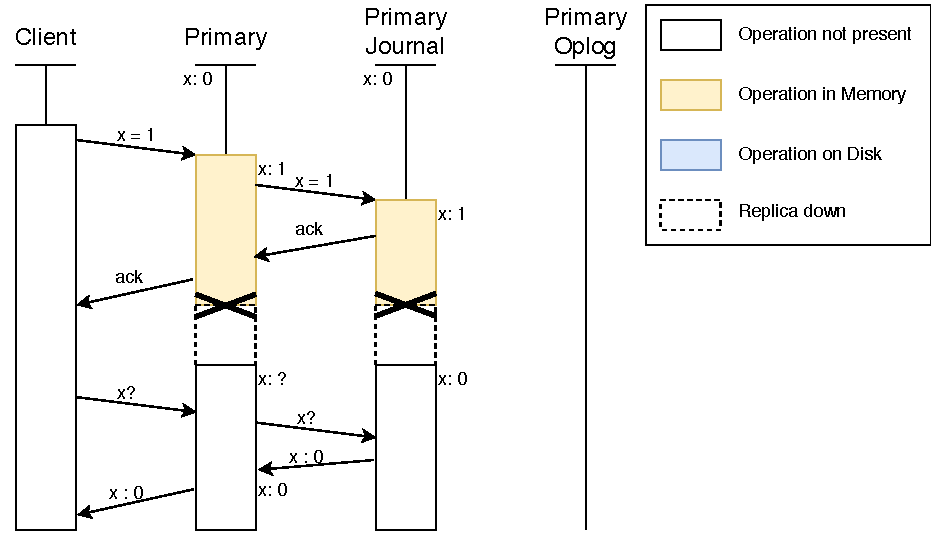
\includegraphics{images/nopersist.pdf}
    \label{fig:nopersist}
    \caption{A time-space diagram of a scenario where a write gets lost due to a failure to persist it on disk}
\end{figure}

This failure relies on two core properties of MongoDB - acknowledging a write before persisting it and only adding a write to the Oplog after flushing it to disk.

Take an operation $o$, with write concern \textit{journaled}, which has just been received by the primary. Currently, the primary stores this operation in memory, performs the operation on the in-memory copy of the data and buffers the write to the journal, but does not yet flush it to disk. Recall that a write is added to the Oplog only \textit{after} it has been flushed to disk. This creates a situation where secondary nodes do not know about a write that has been acknowledged by the primary. As such, if a primary is to crash it will "forget" about $o$ as it was only stored in memory. None of the secondary replicas would have seen $o$ either. A client querying the primary will force it to read the last value of the document operated on from disk. The value returned from the read will not account for the latest operation, which demonstrates the operation has been lost.

Thus, this failure scenario occurs with primary write concern but may also occur with journaled, if the write is buffered instead of being immediately persisted. It will not occur (in a properly implemented MongoDB system) with write concern majority.

\pagebreak
\subsection{Transient Loss via Primary Preferred Read Preference}
\begin{figure}[H]
    \centering
    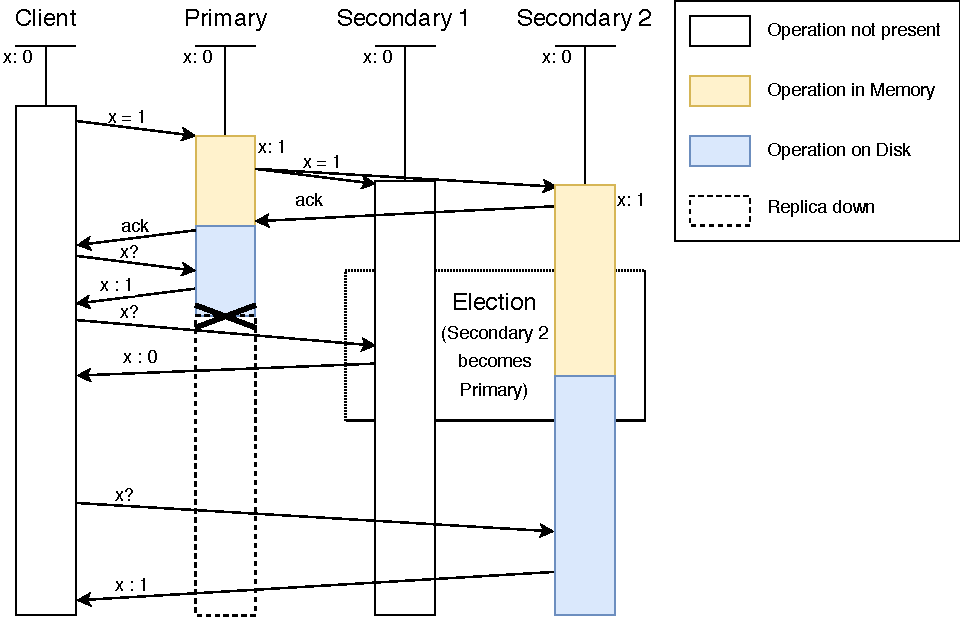
\includegraphics{images/PrimaryPreferred.pdf}
    \label{fig:primarypreferred}
    \caption{A time-space diagram of a scenario where a Majority write concern write gets temporarily lost as a result of the MongoDB client choosing the wrong Secondary to read from.}
\end{figure}

Recall from \prettyref{sec:readpref} that the Primary Preferred read preference will query the secondary if the primary appears to be down, instead of waiting for a primary to respond. The MongoDB client will only query one secondary. This can create a situation where a write will seem to be available, lost and available again. 

Specifically, consider an operation $o$ that was submitted with a majority write concern to the replica set. The primary will acknowledge the write when $\lfloor\frac{|R|}{2}\rfloor$ secondaries also acknowledge the write. This leaves $\lfloor\frac{|R|}{2}\rfloor$ secondaries that may not have acknowledged or even received the write. As such, if the primary is to fail immediately after acknowledging the operation, the MongoDB client has $\frac{\lfloor\frac{|R|}{2}\rfloor - 1}{|R|}$ chance of querying  a secondary that has not seen $o$. Intuitively, this probability reduces with time as more replicas apply the operation to their copy of the data.

If the client is to query the primary, the data returned will have operation $o$ applied to it. Once the primary fails, the MongoDB client has a chance of querying a secondary that has not applied the operation, hence the data returned from that query will not have the operation $o$ applied. Querying the new primary after an election will once again return data with operation $o$ applied. 

As such, Primary Preferred read preference can create instances of transient write loss, where acknowledged operations seem to disappear and reappear during a failure. This scenario can occur in all write concerns, but "all".
\chapter{Experiment Design \& Methodology} \label{chap:experiments}

In this chapter we offer a design and methodology of an experiment and analysis that can quantitatively evaluate the durability of a distributed storage system by measuring the frequency and quantity of write loss under failures. The experiment induces the conditions we identified in \prettyref{chap:det-theory}, and \prettyref{chap:det-results} will report on running the experiments on MongoDB.

\section{Database Contents}

Each document has a simple ID \& value structure as seen in \prettyref{alg:doc}.

\begin{algorithm}
\caption{Example document}
\begin{verbatim}
{
    Id:  5,
    Val: 7
}
\end{verbatim}
\label{alg:doc}
\end{algorithm}

\section{Methodology}

The experiment is set up by creating three identical virtual machines with the database system installed and configured to run in a replica set. We then run a stress test on the replica set using a single client on the host machine which initiates many operations, on separate threads, in parallel. The operations performed are reads, writes and updates on randomly chosen documents with randomly chosen values.

During the run of the experiment, the harness records an execution history, keeping track of each operation performed and error returned by the replica set. Each read, write and update operation is individually recorded into the execution history along with the document id corresponding to the document the operation is performed on,
the timestamp and duration of the operation. Each read record contains the value returned by the database, while the write and update records contain the new value written to the document. Any operations that result in an error are also recorded with the same data.

\begin{figure}
    \begin{CVerbatim}
R,5b9f25ef2644855182a9201c,1042661835,66.689,1537156641143
U,5b9f25ef2644855182a9201c,705768886,1.132,1537156641288
ERR,W,5b9f25f82644855182a92ff2,834995024,22.04,1537156641795
R,5b9f25ef2644855182a9201c,705768886,58.42,1537156641830
    \end{CVerbatim}
    \caption{Sample excerpt of an execution history}
\end{figure}

The experiment is broken into three stages with each stage occupying a third of the experiment time:

\begin{description}
    \item[Standard operation] The virtual machines are started in "Headless" mode and run normally.
    \item[Operating under failure] A failure is induced on the primary. The primary replica disconnects from the replica set initiating an election. 
    \item[Recovery] The failure is reverted and the failed machine is connected back to the replica set.
\end{description}

\section{Failures}

The failures induced during the experiments involve shutting down the primary replica and observing how the secondary nodes behave immediately after the shutdown. The timestamps for when a failure is induced and fixed are also entered into the execution history. 
The following failures are induced in our experiment:

\begin{description}
    \item[Graceful ACPI Shutdown] Sends an ACPI shutdown signal to the virtual machine to trigger a graceful shutdown.
    \item[Hard Poweroff] Simulates an abrupt power failure, which turns the VM off immediately.
\end{description}

Since we focus on crash-tolerant systems, we chose these failures they are supposed to be handled gracefully and correctly by the replica set. This will allow us to find concrete durability failures in the system, that should be possible to prevent within the failure assumptions the system makes. Additionally, they are common system administration scenarios of needing to restart a machine or cutting the power. The recovery flows following these failures will need to re-elect the primary after the failure and, once the failed machine is back up, allow it to "catch up" on the writes which it has not seen.

\section{Workload}
The workload of each experiment consists of three types of operations:

\begin{description}
    \item[Create Document] This operation adds a new document to the collection in the replica set. A new document is created with a value retrieved from a random number generator. Upon acknowledgement of the write from the replica set, its document ID is added to the list of IDs with acknowledged writes.
    \item[Read document] This operation queries the replica set for a document, given its key. The key for the query is chosen randomly from a list of IDs with acknowledged writes. This means, we expect that every query should return a document. Any missing documents are therefore as a result of an error in the replica set.
    \item[Update document] This operation modifies the value of an existing document. The key for the query is chosen randomly from a list of IDs with acknowledged writes and the value is generated using a random number generator.
\end{description}

The primary setting used to vary the workload of the experiment is \textit{write probability}, which determines how often a write operation is issued to the replica set. There are two types of write operations in this experiment - \textit{create document} and \textit{update document}. The decision between which operation to perform is random with equal likelihood.

In addition, we set the Read Concern, Write Concern and Read Preference. This configuration varies between experiments, allowing us to explore the tradeoffs between these configurations and understand which configuration is best for a given scenario.

\section{Execution Analysis}
The execution history produced by each run of the experiment is analysed by Algorithm \ref{alg:eval} to produce the following data:
\begin{description}
    \item[Throughput] The number of successful operations performed during the entire run of the experiment.
    \item[Errors] The number of operations that did not receive a positive acknowledgement, either they got a negative acknowledgement, or they were time out without any acknowledgement.
    \item[Lost Writes] The number of write operations which were lost either temporarily or permanently.
\end{description}

In particular, the algorithm detects when the expected value of the document and value returned from a read are not the same or where the value is missing (denoted by a value of -1). This indicates that a write has either been lost, or that it has been committed but an acknowledgement was not received by the client. We make a distinction between these two cases by keeping track of the write operations that came back as errors to the client which allows us to handle the committed-but-not-acknowledged write and update the state of our analysis as needed. 

\begin{algorithm}
    \caption{Algorithm used for evaluating the execution history}
    \begin{algorithmic}
        \STATE $H \leftarrow$ execution history
        \STATE $t_{fail} \leftarrow$ timestamp of failure induction
        \STATE $t_{fix} \leftarrow$ timestamp of failure repair
        \STATE $D \leftarrow \{\}$ \COMMENT{Lookup of every document's current value}
        \STATE $D_e \leftarrow \{\}$ \COMMENT{Lookup of every write that errored for a document}
        \STATE $E \leftarrow \{\}$ \COMMENT{Set of all errors produced}
        \STATE $M \leftarrow \{\}$ \COMMENT{Set of missing writes}
        \STATE $U \leftarrow \{\}$ \COMMENT{Set of unacknowledged writes}
        \STATE $o \leftarrow 0$ \COMMENT{Number of successful operations}
        \STATE $s \leftarrow $ Normal \COMMENT{Current state of the history (Normal, Failure or Recovery)}

        \FORALL{$h \in H$}
            \IF{$h.time \leq t_{fail}$}
                \STATE $s \leftarrow$ Normal
            \ELSIF{$t_{fail} < h.time \leq t_{fix}$}
                \STATE $s \leftarrow$ Failure
            \ELSE
                \STATE $s \leftarrow$ Recovery
            \ENDIF

            \IF{$h.op =$ Write \OR $h.op =$ Update}
                \STATE $o \leftarrow o+1$
                \STATE $D[h.id] \leftarrow h.val$
            \ELSIF{$h.op =$ Read}
                \STATE $o \leftarrow o+1$
                \IF{$h.val \neq D[h.id]$}
                    \IF{$h.id \in D_e$ \AND $h.val \in D_e[h.id]$}
                        \STATE $U \leftarrow U \cup \{(h.id, h.val, s)\}$
                        \STATE $D[h.id] \leftarrow h.val$
                        \STATE delete $h.val$ from $D_e[h.id]$
                    \ELSE
                        \STATE $M \leftarrow M \cup \{(h.id, h.val, state)\}$
                    \ENDIF
                \ENDIF
            \ELSIF{$h.op =$ Induce}
                \STATE $ s \leftarrow $ Failure
            \ELSIF{$h.op =$ Recover} 
                \STATE $ s \leftarrow $ Recovery
            \ELSIF{$h.op =$ Error}
                \STATE $E \leftarrow E \cup \{(h.err\_op, h.id, h.val, s)\}$
                \IF{$h.err\_op =$ Write \OR $h.err\_op =$ Read}
                    \STATE $D_e[h.id] \leftarrow D_e[h.id] \cup \{h.val\}$
                \ENDIF
            \ENDIF
        \ENDFOR
    \end{algorithmic}
    \label{alg:eval}
\end{algorithm}

Additionally, we also use the execution history to plot the number of different measures against the time of the experiment, bucketed using bins of 1 second.
\chapter{Results} \label{chap:kdur-results}

In this chapter, we present an empirical exploration of time-till-1-durability in MongoDB based on the theory developed in \prettyref{chap:kdur-theory} and proceed to evaluate the results in light of how MongoDB handles write operations.

\section{Environment}
The experiments were performed on the same harness as the one developed in \prettyref{chap:det-results}, using the \textit{Local} read concern and \textit{Primary} read preference. The harness was configured to \textit{not} induce a failure and perform only write operations (using write probability 1). 

\section{Estimating 1-durability}
We ran two experiments, each for 5 minutes. One with write concern \textit{w:1} and one with \textit{journaled}. The execution histories were processed to count the latencies of each operation. The raw results of this collection can be seen in \prettyref{fig:latencies}.

Given that there is a significant difference between the patterns of \textit{w:1} and \textit{journaled} histories, we use the journaled history and apply equation \prettyref{eq:persist} on every operation to derive the time a write becomes 1-durable. Given that VirtualBox networking is very stable, we subtract the average ping latency to the primary from every operation to determine the time that operation became 1-durable. A comparison between 1-durability and \textit{w:1} write acknowledgement can be found in \prettyref{fig:cdf}.

To further clarify the differences between \textit{w:1} and 1-durability, we present a chart of the difference between the two cumulative plots in \prettyref{fig:diff}.

\begin{figure}
    \centering        
    %% Creator: Matplotlib, PGF backend
%%
%% To include the figure in your LaTeX document, write
%%   \input{<filename>.pgf}
%%
%% Make sure the required packages are loaded in your preamble
%%   \usepackage{pgf}
%%
%% Figures using additional raster images can only be included by \input if
%% they are in the same directory as the main LaTeX file. For loading figures
%% from other directories you can use the `import` package
%%   \usepackage{import}
%% and then include the figures with
%%   \import{<path to file>}{<filename>.pgf}
%%
%% Matplotlib used the following preamble
%%   \usepackage[utf8x]{inputenc}
%%   \usepackage[T1]{fontenc}
%%   \usepackage{lmodern}
%%
\begingroup%
\makeatletter%
\begin{pgfpicture}%
\pgfpathrectangle{\pgfpointorigin}{\pgfqpoint{6.400000in}{4.800000in}}%
\pgfusepath{use as bounding box, clip}%
\begin{pgfscope}%
\pgfsetbuttcap%
\pgfsetmiterjoin%
\definecolor{currentfill}{rgb}{1.000000,1.000000,1.000000}%
\pgfsetfillcolor{currentfill}%
\pgfsetlinewidth{0.000000pt}%
\definecolor{currentstroke}{rgb}{1.000000,1.000000,1.000000}%
\pgfsetstrokecolor{currentstroke}%
\pgfsetdash{}{0pt}%
\pgfpathmoveto{\pgfqpoint{0.000000in}{0.000000in}}%
\pgfpathlineto{\pgfqpoint{6.400000in}{0.000000in}}%
\pgfpathlineto{\pgfqpoint{6.400000in}{4.800000in}}%
\pgfpathlineto{\pgfqpoint{0.000000in}{4.800000in}}%
\pgfpathclose%
\pgfusepath{fill}%
\end{pgfscope}%
\begin{pgfscope}%
\pgfsetbuttcap%
\pgfsetmiterjoin%
\definecolor{currentfill}{rgb}{1.000000,1.000000,1.000000}%
\pgfsetfillcolor{currentfill}%
\pgfsetlinewidth{0.000000pt}%
\definecolor{currentstroke}{rgb}{0.000000,0.000000,0.000000}%
\pgfsetstrokecolor{currentstroke}%
\pgfsetstrokeopacity{0.000000}%
\pgfsetdash{}{0pt}%
\pgfpathmoveto{\pgfqpoint{0.800000in}{0.528000in}}%
\pgfpathlineto{\pgfqpoint{5.760000in}{0.528000in}}%
\pgfpathlineto{\pgfqpoint{5.760000in}{4.224000in}}%
\pgfpathlineto{\pgfqpoint{0.800000in}{4.224000in}}%
\pgfpathclose%
\pgfusepath{fill}%
\end{pgfscope}%
\begin{pgfscope}%
\pgfsetbuttcap%
\pgfsetroundjoin%
\definecolor{currentfill}{rgb}{0.000000,0.000000,0.000000}%
\pgfsetfillcolor{currentfill}%
\pgfsetlinewidth{0.803000pt}%
\definecolor{currentstroke}{rgb}{0.000000,0.000000,0.000000}%
\pgfsetstrokecolor{currentstroke}%
\pgfsetdash{}{0pt}%
\pgfsys@defobject{currentmarker}{\pgfqpoint{0.000000in}{-0.048611in}}{\pgfqpoint{0.000000in}{0.000000in}}{%
\pgfpathmoveto{\pgfqpoint{0.000000in}{0.000000in}}%
\pgfpathlineto{\pgfqpoint{0.000000in}{-0.048611in}}%
\pgfusepath{stroke,fill}%
}%
\begin{pgfscope}%
\pgfsys@transformshift{1.020936in}{0.528000in}%
\pgfsys@useobject{currentmarker}{}%
\end{pgfscope}%
\end{pgfscope}%
\begin{pgfscope}%
\pgftext[x=1.020936in,y=0.430778in,,top]{\fontsize{11.000000}{13.200000}\selectfont \(\displaystyle 0\)}%
\end{pgfscope}%
\begin{pgfscope}%
\pgfsetbuttcap%
\pgfsetroundjoin%
\definecolor{currentfill}{rgb}{0.000000,0.000000,0.000000}%
\pgfsetfillcolor{currentfill}%
\pgfsetlinewidth{0.803000pt}%
\definecolor{currentstroke}{rgb}{0.000000,0.000000,0.000000}%
\pgfsetstrokecolor{currentstroke}%
\pgfsetdash{}{0pt}%
\pgfsys@defobject{currentmarker}{\pgfqpoint{0.000000in}{-0.048611in}}{\pgfqpoint{0.000000in}{0.000000in}}{%
\pgfpathmoveto{\pgfqpoint{0.000000in}{0.000000in}}%
\pgfpathlineto{\pgfqpoint{0.000000in}{-0.048611in}}%
\pgfusepath{stroke,fill}%
}%
\begin{pgfscope}%
\pgfsys@transformshift{1.924562in}{0.528000in}%
\pgfsys@useobject{currentmarker}{}%
\end{pgfscope}%
\end{pgfscope}%
\begin{pgfscope}%
\pgftext[x=1.924562in,y=0.430778in,,top]{\fontsize{11.000000}{13.200000}\selectfont \(\displaystyle 200\)}%
\end{pgfscope}%
\begin{pgfscope}%
\pgfsetbuttcap%
\pgfsetroundjoin%
\definecolor{currentfill}{rgb}{0.000000,0.000000,0.000000}%
\pgfsetfillcolor{currentfill}%
\pgfsetlinewidth{0.803000pt}%
\definecolor{currentstroke}{rgb}{0.000000,0.000000,0.000000}%
\pgfsetstrokecolor{currentstroke}%
\pgfsetdash{}{0pt}%
\pgfsys@defobject{currentmarker}{\pgfqpoint{0.000000in}{-0.048611in}}{\pgfqpoint{0.000000in}{0.000000in}}{%
\pgfpathmoveto{\pgfqpoint{0.000000in}{0.000000in}}%
\pgfpathlineto{\pgfqpoint{0.000000in}{-0.048611in}}%
\pgfusepath{stroke,fill}%
}%
\begin{pgfscope}%
\pgfsys@transformshift{2.828187in}{0.528000in}%
\pgfsys@useobject{currentmarker}{}%
\end{pgfscope}%
\end{pgfscope}%
\begin{pgfscope}%
\pgftext[x=2.828187in,y=0.430778in,,top]{\fontsize{11.000000}{13.200000}\selectfont \(\displaystyle 400\)}%
\end{pgfscope}%
\begin{pgfscope}%
\pgfsetbuttcap%
\pgfsetroundjoin%
\definecolor{currentfill}{rgb}{0.000000,0.000000,0.000000}%
\pgfsetfillcolor{currentfill}%
\pgfsetlinewidth{0.803000pt}%
\definecolor{currentstroke}{rgb}{0.000000,0.000000,0.000000}%
\pgfsetstrokecolor{currentstroke}%
\pgfsetdash{}{0pt}%
\pgfsys@defobject{currentmarker}{\pgfqpoint{0.000000in}{-0.048611in}}{\pgfqpoint{0.000000in}{0.000000in}}{%
\pgfpathmoveto{\pgfqpoint{0.000000in}{0.000000in}}%
\pgfpathlineto{\pgfqpoint{0.000000in}{-0.048611in}}%
\pgfusepath{stroke,fill}%
}%
\begin{pgfscope}%
\pgfsys@transformshift{3.731813in}{0.528000in}%
\pgfsys@useobject{currentmarker}{}%
\end{pgfscope}%
\end{pgfscope}%
\begin{pgfscope}%
\pgftext[x=3.731813in,y=0.430778in,,top]{\fontsize{11.000000}{13.200000}\selectfont \(\displaystyle 600\)}%
\end{pgfscope}%
\begin{pgfscope}%
\pgfsetbuttcap%
\pgfsetroundjoin%
\definecolor{currentfill}{rgb}{0.000000,0.000000,0.000000}%
\pgfsetfillcolor{currentfill}%
\pgfsetlinewidth{0.803000pt}%
\definecolor{currentstroke}{rgb}{0.000000,0.000000,0.000000}%
\pgfsetstrokecolor{currentstroke}%
\pgfsetdash{}{0pt}%
\pgfsys@defobject{currentmarker}{\pgfqpoint{0.000000in}{-0.048611in}}{\pgfqpoint{0.000000in}{0.000000in}}{%
\pgfpathmoveto{\pgfqpoint{0.000000in}{0.000000in}}%
\pgfpathlineto{\pgfqpoint{0.000000in}{-0.048611in}}%
\pgfusepath{stroke,fill}%
}%
\begin{pgfscope}%
\pgfsys@transformshift{4.635438in}{0.528000in}%
\pgfsys@useobject{currentmarker}{}%
\end{pgfscope}%
\end{pgfscope}%
\begin{pgfscope}%
\pgftext[x=4.635438in,y=0.430778in,,top]{\fontsize{11.000000}{13.200000}\selectfont \(\displaystyle 800\)}%
\end{pgfscope}%
\begin{pgfscope}%
\pgfsetbuttcap%
\pgfsetroundjoin%
\definecolor{currentfill}{rgb}{0.000000,0.000000,0.000000}%
\pgfsetfillcolor{currentfill}%
\pgfsetlinewidth{0.803000pt}%
\definecolor{currentstroke}{rgb}{0.000000,0.000000,0.000000}%
\pgfsetstrokecolor{currentstroke}%
\pgfsetdash{}{0pt}%
\pgfsys@defobject{currentmarker}{\pgfqpoint{0.000000in}{-0.048611in}}{\pgfqpoint{0.000000in}{0.000000in}}{%
\pgfpathmoveto{\pgfqpoint{0.000000in}{0.000000in}}%
\pgfpathlineto{\pgfqpoint{0.000000in}{-0.048611in}}%
\pgfusepath{stroke,fill}%
}%
\begin{pgfscope}%
\pgfsys@transformshift{5.539064in}{0.528000in}%
\pgfsys@useobject{currentmarker}{}%
\end{pgfscope}%
\end{pgfscope}%
\begin{pgfscope}%
\pgftext[x=5.539064in,y=0.430778in,,top]{\fontsize{11.000000}{13.200000}\selectfont \(\displaystyle 1000\)}%
\end{pgfscope}%
\begin{pgfscope}%
\pgftext[x=3.280000in,y=0.240271in,,top]{\fontsize{11.000000}{13.200000}\selectfont Latency (in milliseconds)}%
\end{pgfscope}%
\begin{pgfscope}%
\pgfsetbuttcap%
\pgfsetroundjoin%
\definecolor{currentfill}{rgb}{0.000000,0.000000,0.000000}%
\pgfsetfillcolor{currentfill}%
\pgfsetlinewidth{0.803000pt}%
\definecolor{currentstroke}{rgb}{0.000000,0.000000,0.000000}%
\pgfsetstrokecolor{currentstroke}%
\pgfsetdash{}{0pt}%
\pgfsys@defobject{currentmarker}{\pgfqpoint{-0.048611in}{0.000000in}}{\pgfqpoint{0.000000in}{0.000000in}}{%
\pgfpathmoveto{\pgfqpoint{0.000000in}{0.000000in}}%
\pgfpathlineto{\pgfqpoint{-0.048611in}{0.000000in}}%
\pgfusepath{stroke,fill}%
}%
\begin{pgfscope}%
\pgfsys@transformshift{0.800000in}{0.696000in}%
\pgfsys@useobject{currentmarker}{}%
\end{pgfscope}%
\end{pgfscope}%
\begin{pgfscope}%
\pgftext[x=0.627981in,y=0.643378in,left,base]{\fontsize{11.000000}{13.200000}\selectfont \(\displaystyle 0\)}%
\end{pgfscope}%
\begin{pgfscope}%
\pgfsetbuttcap%
\pgfsetroundjoin%
\definecolor{currentfill}{rgb}{0.000000,0.000000,0.000000}%
\pgfsetfillcolor{currentfill}%
\pgfsetlinewidth{0.803000pt}%
\definecolor{currentstroke}{rgb}{0.000000,0.000000,0.000000}%
\pgfsetstrokecolor{currentstroke}%
\pgfsetdash{}{0pt}%
\pgfsys@defobject{currentmarker}{\pgfqpoint{-0.048611in}{0.000000in}}{\pgfqpoint{0.000000in}{0.000000in}}{%
\pgfpathmoveto{\pgfqpoint{0.000000in}{0.000000in}}%
\pgfpathlineto{\pgfqpoint{-0.048611in}{0.000000in}}%
\pgfusepath{stroke,fill}%
}%
\begin{pgfscope}%
\pgfsys@transformshift{0.800000in}{1.129492in}%
\pgfsys@useobject{currentmarker}{}%
\end{pgfscope}%
\end{pgfscope}%
\begin{pgfscope}%
\pgftext[x=0.403588in,y=1.076870in,left,base]{\fontsize{11.000000}{13.200000}\selectfont \(\displaystyle 1000\)}%
\end{pgfscope}%
\begin{pgfscope}%
\pgfsetbuttcap%
\pgfsetroundjoin%
\definecolor{currentfill}{rgb}{0.000000,0.000000,0.000000}%
\pgfsetfillcolor{currentfill}%
\pgfsetlinewidth{0.803000pt}%
\definecolor{currentstroke}{rgb}{0.000000,0.000000,0.000000}%
\pgfsetstrokecolor{currentstroke}%
\pgfsetdash{}{0pt}%
\pgfsys@defobject{currentmarker}{\pgfqpoint{-0.048611in}{0.000000in}}{\pgfqpoint{0.000000in}{0.000000in}}{%
\pgfpathmoveto{\pgfqpoint{0.000000in}{0.000000in}}%
\pgfpathlineto{\pgfqpoint{-0.048611in}{0.000000in}}%
\pgfusepath{stroke,fill}%
}%
\begin{pgfscope}%
\pgfsys@transformshift{0.800000in}{1.562985in}%
\pgfsys@useobject{currentmarker}{}%
\end{pgfscope}%
\end{pgfscope}%
\begin{pgfscope}%
\pgftext[x=0.403588in,y=1.510363in,left,base]{\fontsize{11.000000}{13.200000}\selectfont \(\displaystyle 2000\)}%
\end{pgfscope}%
\begin{pgfscope}%
\pgfsetbuttcap%
\pgfsetroundjoin%
\definecolor{currentfill}{rgb}{0.000000,0.000000,0.000000}%
\pgfsetfillcolor{currentfill}%
\pgfsetlinewidth{0.803000pt}%
\definecolor{currentstroke}{rgb}{0.000000,0.000000,0.000000}%
\pgfsetstrokecolor{currentstroke}%
\pgfsetdash{}{0pt}%
\pgfsys@defobject{currentmarker}{\pgfqpoint{-0.048611in}{0.000000in}}{\pgfqpoint{0.000000in}{0.000000in}}{%
\pgfpathmoveto{\pgfqpoint{0.000000in}{0.000000in}}%
\pgfpathlineto{\pgfqpoint{-0.048611in}{0.000000in}}%
\pgfusepath{stroke,fill}%
}%
\begin{pgfscope}%
\pgfsys@transformshift{0.800000in}{1.996477in}%
\pgfsys@useobject{currentmarker}{}%
\end{pgfscope}%
\end{pgfscope}%
\begin{pgfscope}%
\pgftext[x=0.403588in,y=1.943855in,left,base]{\fontsize{11.000000}{13.200000}\selectfont \(\displaystyle 3000\)}%
\end{pgfscope}%
\begin{pgfscope}%
\pgfsetbuttcap%
\pgfsetroundjoin%
\definecolor{currentfill}{rgb}{0.000000,0.000000,0.000000}%
\pgfsetfillcolor{currentfill}%
\pgfsetlinewidth{0.803000pt}%
\definecolor{currentstroke}{rgb}{0.000000,0.000000,0.000000}%
\pgfsetstrokecolor{currentstroke}%
\pgfsetdash{}{0pt}%
\pgfsys@defobject{currentmarker}{\pgfqpoint{-0.048611in}{0.000000in}}{\pgfqpoint{0.000000in}{0.000000in}}{%
\pgfpathmoveto{\pgfqpoint{0.000000in}{0.000000in}}%
\pgfpathlineto{\pgfqpoint{-0.048611in}{0.000000in}}%
\pgfusepath{stroke,fill}%
}%
\begin{pgfscope}%
\pgfsys@transformshift{0.800000in}{2.429970in}%
\pgfsys@useobject{currentmarker}{}%
\end{pgfscope}%
\end{pgfscope}%
\begin{pgfscope}%
\pgftext[x=0.403588in,y=2.377348in,left,base]{\fontsize{11.000000}{13.200000}\selectfont \(\displaystyle 4000\)}%
\end{pgfscope}%
\begin{pgfscope}%
\pgfsetbuttcap%
\pgfsetroundjoin%
\definecolor{currentfill}{rgb}{0.000000,0.000000,0.000000}%
\pgfsetfillcolor{currentfill}%
\pgfsetlinewidth{0.803000pt}%
\definecolor{currentstroke}{rgb}{0.000000,0.000000,0.000000}%
\pgfsetstrokecolor{currentstroke}%
\pgfsetdash{}{0pt}%
\pgfsys@defobject{currentmarker}{\pgfqpoint{-0.048611in}{0.000000in}}{\pgfqpoint{0.000000in}{0.000000in}}{%
\pgfpathmoveto{\pgfqpoint{0.000000in}{0.000000in}}%
\pgfpathlineto{\pgfqpoint{-0.048611in}{0.000000in}}%
\pgfusepath{stroke,fill}%
}%
\begin{pgfscope}%
\pgfsys@transformshift{0.800000in}{2.863462in}%
\pgfsys@useobject{currentmarker}{}%
\end{pgfscope}%
\end{pgfscope}%
\begin{pgfscope}%
\pgftext[x=0.403588in,y=2.810840in,left,base]{\fontsize{11.000000}{13.200000}\selectfont \(\displaystyle 5000\)}%
\end{pgfscope}%
\begin{pgfscope}%
\pgfsetbuttcap%
\pgfsetroundjoin%
\definecolor{currentfill}{rgb}{0.000000,0.000000,0.000000}%
\pgfsetfillcolor{currentfill}%
\pgfsetlinewidth{0.803000pt}%
\definecolor{currentstroke}{rgb}{0.000000,0.000000,0.000000}%
\pgfsetstrokecolor{currentstroke}%
\pgfsetdash{}{0pt}%
\pgfsys@defobject{currentmarker}{\pgfqpoint{-0.048611in}{0.000000in}}{\pgfqpoint{0.000000in}{0.000000in}}{%
\pgfpathmoveto{\pgfqpoint{0.000000in}{0.000000in}}%
\pgfpathlineto{\pgfqpoint{-0.048611in}{0.000000in}}%
\pgfusepath{stroke,fill}%
}%
\begin{pgfscope}%
\pgfsys@transformshift{0.800000in}{3.296955in}%
\pgfsys@useobject{currentmarker}{}%
\end{pgfscope}%
\end{pgfscope}%
\begin{pgfscope}%
\pgftext[x=0.403588in,y=3.244332in,left,base]{\fontsize{11.000000}{13.200000}\selectfont \(\displaystyle 6000\)}%
\end{pgfscope}%
\begin{pgfscope}%
\pgfsetbuttcap%
\pgfsetroundjoin%
\definecolor{currentfill}{rgb}{0.000000,0.000000,0.000000}%
\pgfsetfillcolor{currentfill}%
\pgfsetlinewidth{0.803000pt}%
\definecolor{currentstroke}{rgb}{0.000000,0.000000,0.000000}%
\pgfsetstrokecolor{currentstroke}%
\pgfsetdash{}{0pt}%
\pgfsys@defobject{currentmarker}{\pgfqpoint{-0.048611in}{0.000000in}}{\pgfqpoint{0.000000in}{0.000000in}}{%
\pgfpathmoveto{\pgfqpoint{0.000000in}{0.000000in}}%
\pgfpathlineto{\pgfqpoint{-0.048611in}{0.000000in}}%
\pgfusepath{stroke,fill}%
}%
\begin{pgfscope}%
\pgfsys@transformshift{0.800000in}{3.730447in}%
\pgfsys@useobject{currentmarker}{}%
\end{pgfscope}%
\end{pgfscope}%
\begin{pgfscope}%
\pgftext[x=0.403588in,y=3.677825in,left,base]{\fontsize{11.000000}{13.200000}\selectfont \(\displaystyle 7000\)}%
\end{pgfscope}%
\begin{pgfscope}%
\pgfsetbuttcap%
\pgfsetroundjoin%
\definecolor{currentfill}{rgb}{0.000000,0.000000,0.000000}%
\pgfsetfillcolor{currentfill}%
\pgfsetlinewidth{0.803000pt}%
\definecolor{currentstroke}{rgb}{0.000000,0.000000,0.000000}%
\pgfsetstrokecolor{currentstroke}%
\pgfsetdash{}{0pt}%
\pgfsys@defobject{currentmarker}{\pgfqpoint{-0.048611in}{0.000000in}}{\pgfqpoint{0.000000in}{0.000000in}}{%
\pgfpathmoveto{\pgfqpoint{0.000000in}{0.000000in}}%
\pgfpathlineto{\pgfqpoint{-0.048611in}{0.000000in}}%
\pgfusepath{stroke,fill}%
}%
\begin{pgfscope}%
\pgfsys@transformshift{0.800000in}{4.163940in}%
\pgfsys@useobject{currentmarker}{}%
\end{pgfscope}%
\end{pgfscope}%
\begin{pgfscope}%
\pgftext[x=0.403588in,y=4.111317in,left,base]{\fontsize{11.000000}{13.200000}\selectfont \(\displaystyle 8000\)}%
\end{pgfscope}%
\begin{pgfscope}%
\pgftext[x=0.348033in,y=2.376000in,,bottom,rotate=90.000000]{\fontsize{11.000000}{13.200000}\selectfont Number of operations}%
\end{pgfscope}%
\begin{pgfscope}%
\pgfpathrectangle{\pgfqpoint{0.800000in}{0.528000in}}{\pgfqpoint{4.960000in}{3.696000in}}%
\pgfusepath{clip}%
\pgfsetrectcap%
\pgfsetroundjoin%
\pgfsetlinewidth{1.505625pt}%
\definecolor{currentstroke}{rgb}{0.121569,0.466667,0.705882}%
\pgfsetstrokecolor{currentstroke}%
\pgfsetdash{}{0pt}%
\pgfpathmoveto{\pgfqpoint{1.025455in}{1.752855in}}%
\pgfpathlineto{\pgfqpoint{1.029973in}{1.641447in}}%
\pgfpathlineto{\pgfqpoint{1.034491in}{1.632344in}}%
\pgfpathlineto{\pgfqpoint{1.039009in}{1.615871in}}%
\pgfpathlineto{\pgfqpoint{1.043527in}{1.570788in}}%
\pgfpathlineto{\pgfqpoint{1.048045in}{1.623674in}}%
\pgfpathlineto{\pgfqpoint{1.052563in}{1.613270in}}%
\pgfpathlineto{\pgfqpoint{1.061600in}{1.502296in}}%
\pgfpathlineto{\pgfqpoint{1.066118in}{1.454178in}}%
\pgfpathlineto{\pgfqpoint{1.070636in}{1.436839in}}%
\pgfpathlineto{\pgfqpoint{1.075154in}{1.357943in}}%
\pgfpathlineto{\pgfqpoint{1.079672in}{1.379184in}}%
\pgfpathlineto{\pgfqpoint{1.084190in}{1.332367in}}%
\pgfpathlineto{\pgfqpoint{1.097745in}{1.240467in}}%
\pgfpathlineto{\pgfqpoint{1.102263in}{1.184979in}}%
\pgfpathlineto{\pgfqpoint{1.106781in}{1.148133in}}%
\pgfpathlineto{\pgfqpoint{1.111299in}{1.142064in}}%
\pgfpathlineto{\pgfqpoint{1.115817in}{1.080941in}}%
\pgfpathlineto{\pgfqpoint{1.120335in}{1.077473in}}%
\pgfpathlineto{\pgfqpoint{1.124853in}{1.051897in}}%
\pgfpathlineto{\pgfqpoint{1.129371in}{1.044961in}}%
\pgfpathlineto{\pgfqpoint{1.133890in}{1.019819in}}%
\pgfpathlineto{\pgfqpoint{1.138408in}{1.002479in}}%
\pgfpathlineto{\pgfqpoint{1.147444in}{0.945692in}}%
\pgfpathlineto{\pgfqpoint{1.151962in}{0.924451in}}%
\pgfpathlineto{\pgfqpoint{1.156480in}{0.941790in}}%
\pgfpathlineto{\pgfqpoint{1.160998in}{0.890638in}}%
\pgfpathlineto{\pgfqpoint{1.165516in}{0.902342in}}%
\pgfpathlineto{\pgfqpoint{1.174553in}{0.842087in}}%
\pgfpathlineto{\pgfqpoint{1.179071in}{0.838186in}}%
\pgfpathlineto{\pgfqpoint{1.183589in}{0.841220in}}%
\pgfpathlineto{\pgfqpoint{1.188107in}{0.829082in}}%
\pgfpathlineto{\pgfqpoint{1.192625in}{0.837752in}}%
\pgfpathlineto{\pgfqpoint{1.197143in}{0.825181in}}%
\pgfpathlineto{\pgfqpoint{1.201662in}{0.835151in}}%
\pgfpathlineto{\pgfqpoint{1.206180in}{0.827782in}}%
\pgfpathlineto{\pgfqpoint{1.210698in}{0.845988in}}%
\pgfpathlineto{\pgfqpoint{1.215216in}{0.857693in}}%
\pgfpathlineto{\pgfqpoint{1.219734in}{0.886303in}}%
\pgfpathlineto{\pgfqpoint{1.224252in}{0.924451in}}%
\pgfpathlineto{\pgfqpoint{1.228770in}{0.944825in}}%
\pgfpathlineto{\pgfqpoint{1.237807in}{1.063602in}}%
\pgfpathlineto{\pgfqpoint{1.242325in}{1.126025in}}%
\pgfpathlineto{\pgfqpoint{1.246843in}{1.347973in}}%
\pgfpathlineto{\pgfqpoint{1.251361in}{1.315461in}}%
\pgfpathlineto{\pgfqpoint{1.255879in}{1.435105in}}%
\pgfpathlineto{\pgfqpoint{1.260397in}{1.496661in}}%
\pgfpathlineto{\pgfqpoint{1.264915in}{1.742884in}}%
\pgfpathlineto{\pgfqpoint{1.273952in}{2.383153in}}%
\pgfpathlineto{\pgfqpoint{1.278470in}{2.811877in}}%
\pgfpathlineto{\pgfqpoint{1.282988in}{2.925018in}}%
\pgfpathlineto{\pgfqpoint{1.287506in}{2.944959in}}%
\pgfpathlineto{\pgfqpoint{1.292024in}{3.285684in}}%
\pgfpathlineto{\pgfqpoint{1.296542in}{3.500696in}}%
\pgfpathlineto{\pgfqpoint{1.301060in}{3.795471in}}%
\pgfpathlineto{\pgfqpoint{1.305578in}{3.819747in}}%
\pgfpathlineto{\pgfqpoint{1.310097in}{3.826249in}}%
\pgfpathlineto{\pgfqpoint{1.314615in}{4.056000in}}%
\pgfpathlineto{\pgfqpoint{1.319133in}{3.809343in}}%
\pgfpathlineto{\pgfqpoint{1.323651in}{3.720477in}}%
\pgfpathlineto{\pgfqpoint{1.328169in}{3.785934in}}%
\pgfpathlineto{\pgfqpoint{1.332687in}{3.953262in}}%
\pgfpathlineto{\pgfqpoint{1.337205in}{4.017853in}}%
\pgfpathlineto{\pgfqpoint{1.341723in}{4.033458in}}%
\pgfpathlineto{\pgfqpoint{1.346242in}{3.977104in}}%
\pgfpathlineto{\pgfqpoint{1.355278in}{3.625975in}}%
\pgfpathlineto{\pgfqpoint{1.359796in}{3.322097in}}%
\pgfpathlineto{\pgfqpoint{1.364314in}{3.151735in}}%
\pgfpathlineto{\pgfqpoint{1.368832in}{2.882969in}}%
\pgfpathlineto{\pgfqpoint{1.391423in}{2.148200in}}%
\pgfpathlineto{\pgfqpoint{1.400459in}{1.983906in}}%
\pgfpathlineto{\pgfqpoint{1.404977in}{1.849957in}}%
\pgfpathlineto{\pgfqpoint{1.414013in}{1.676993in}}%
\pgfpathlineto{\pgfqpoint{1.423050in}{1.565152in}}%
\pgfpathlineto{\pgfqpoint{1.427568in}{1.466316in}}%
\pgfpathlineto{\pgfqpoint{1.432086in}{1.421666in}}%
\pgfpathlineto{\pgfqpoint{1.436604in}{1.327599in}}%
\pgfpathlineto{\pgfqpoint{1.441122in}{1.269077in}}%
\pgfpathlineto{\pgfqpoint{1.445640in}{1.277747in}}%
\pgfpathlineto{\pgfqpoint{1.450158in}{1.276013in}}%
\pgfpathlineto{\pgfqpoint{1.454677in}{1.243067in}}%
\pgfpathlineto{\pgfqpoint{1.459195in}{1.229629in}}%
\pgfpathlineto{\pgfqpoint{1.463713in}{1.184979in}}%
\pgfpathlineto{\pgfqpoint{1.468231in}{1.108251in}}%
\pgfpathlineto{\pgfqpoint{1.472749in}{1.091345in}}%
\pgfpathlineto{\pgfqpoint{1.477267in}{1.093513in}}%
\pgfpathlineto{\pgfqpoint{1.481785in}{1.081375in}}%
\pgfpathlineto{\pgfqpoint{1.490822in}{0.973435in}}%
\pgfpathlineto{\pgfqpoint{1.495340in}{0.980371in}}%
\pgfpathlineto{\pgfqpoint{1.499858in}{1.012016in}}%
\pgfpathlineto{\pgfqpoint{1.504376in}{0.963898in}}%
\pgfpathlineto{\pgfqpoint{1.508894in}{0.977337in}}%
\pgfpathlineto{\pgfqpoint{1.513412in}{1.004647in}}%
\pgfpathlineto{\pgfqpoint{1.517930in}{1.020252in}}%
\pgfpathlineto{\pgfqpoint{1.522449in}{1.025454in}}%
\pgfpathlineto{\pgfqpoint{1.526967in}{1.078774in}}%
\pgfpathlineto{\pgfqpoint{1.531485in}{1.110852in}}%
\pgfpathlineto{\pgfqpoint{1.536003in}{1.189748in}}%
\pgfpathlineto{\pgfqpoint{1.540521in}{1.138162in}}%
\pgfpathlineto{\pgfqpoint{1.545039in}{1.237432in}}%
\pgfpathlineto{\pgfqpoint{1.554075in}{1.305057in}}%
\pgfpathlineto{\pgfqpoint{1.558594in}{1.378317in}}%
\pgfpathlineto{\pgfqpoint{1.563112in}{1.471951in}}%
\pgfpathlineto{\pgfqpoint{1.567630in}{1.603300in}}%
\pgfpathlineto{\pgfqpoint{1.572148in}{1.550847in}}%
\pgfpathlineto{\pgfqpoint{1.576666in}{1.672658in}}%
\pgfpathlineto{\pgfqpoint{1.581184in}{1.702136in}}%
\pgfpathlineto{\pgfqpoint{1.585702in}{1.791435in}}%
\pgfpathlineto{\pgfqpoint{1.590220in}{1.761091in}}%
\pgfpathlineto{\pgfqpoint{1.599257in}{1.924084in}}%
\pgfpathlineto{\pgfqpoint{1.612811in}{2.146899in}}%
\pgfpathlineto{\pgfqpoint{1.617329in}{2.258307in}}%
\pgfpathlineto{\pgfqpoint{1.621847in}{2.423467in}}%
\pgfpathlineto{\pgfqpoint{1.626365in}{2.496294in}}%
\pgfpathlineto{\pgfqpoint{1.630884in}{2.638480in}}%
\pgfpathlineto{\pgfqpoint{1.635402in}{2.709572in}}%
\pgfpathlineto{\pgfqpoint{1.639920in}{2.857827in}}%
\pgfpathlineto{\pgfqpoint{1.644438in}{2.914181in}}%
\pgfpathlineto{\pgfqpoint{1.648956in}{3.095814in}}%
\pgfpathlineto{\pgfqpoint{1.653474in}{2.964033in}}%
\pgfpathlineto{\pgfqpoint{1.657992in}{3.016485in}}%
\pgfpathlineto{\pgfqpoint{1.662510in}{3.015185in}}%
\pgfpathlineto{\pgfqpoint{1.667029in}{2.932821in}}%
\pgfpathlineto{\pgfqpoint{1.671547in}{2.747286in}}%
\pgfpathlineto{\pgfqpoint{1.676065in}{2.692233in}}%
\pgfpathlineto{\pgfqpoint{1.685101in}{2.489792in}}%
\pgfpathlineto{\pgfqpoint{1.689619in}{2.528373in}}%
\pgfpathlineto{\pgfqpoint{1.694137in}{2.403527in}}%
\pgfpathlineto{\pgfqpoint{1.698655in}{2.352808in}}%
\pgfpathlineto{\pgfqpoint{1.703174in}{2.323764in}}%
\pgfpathlineto{\pgfqpoint{1.707692in}{2.322464in}}%
\pgfpathlineto{\pgfqpoint{1.716728in}{2.035925in}}%
\pgfpathlineto{\pgfqpoint{1.721246in}{2.004280in}}%
\pgfpathlineto{\pgfqpoint{1.725764in}{1.848656in}}%
\pgfpathlineto{\pgfqpoint{1.730282in}{1.737249in}}%
\pgfpathlineto{\pgfqpoint{1.734801in}{1.731180in}}%
\pgfpathlineto{\pgfqpoint{1.739319in}{1.646215in}}%
\pgfpathlineto{\pgfqpoint{1.748355in}{1.534808in}}%
\pgfpathlineto{\pgfqpoint{1.752873in}{1.513133in}}%
\pgfpathlineto{\pgfqpoint{1.757391in}{1.441607in}}%
\pgfpathlineto{\pgfqpoint{1.766427in}{1.376583in}}%
\pgfpathlineto{\pgfqpoint{1.770946in}{1.371815in}}%
\pgfpathlineto{\pgfqpoint{1.775464in}{1.348406in}}%
\pgfpathlineto{\pgfqpoint{1.779982in}{1.292919in}}%
\pgfpathlineto{\pgfqpoint{1.784500in}{1.255205in}}%
\pgfpathlineto{\pgfqpoint{1.789018in}{1.234831in}}%
\pgfpathlineto{\pgfqpoint{1.793536in}{1.250870in}}%
\pgfpathlineto{\pgfqpoint{1.798054in}{1.214890in}}%
\pgfpathlineto{\pgfqpoint{1.802572in}{1.282949in}}%
\pgfpathlineto{\pgfqpoint{1.807091in}{1.157669in}}%
\pgfpathlineto{\pgfqpoint{1.811609in}{1.167206in}}%
\pgfpathlineto{\pgfqpoint{1.820645in}{1.200585in}}%
\pgfpathlineto{\pgfqpoint{1.825163in}{1.212290in}}%
\pgfpathlineto{\pgfqpoint{1.829681in}{1.228762in}}%
\pgfpathlineto{\pgfqpoint{1.834199in}{1.258240in}}%
\pgfpathlineto{\pgfqpoint{1.838717in}{1.209689in}}%
\pgfpathlineto{\pgfqpoint{1.843236in}{1.213156in}}%
\pgfpathlineto{\pgfqpoint{1.847754in}{1.293353in}}%
\pgfpathlineto{\pgfqpoint{1.852272in}{1.214890in}}%
\pgfpathlineto{\pgfqpoint{1.856790in}{1.219225in}}%
\pgfpathlineto{\pgfqpoint{1.861308in}{1.263008in}}%
\pgfpathlineto{\pgfqpoint{1.865826in}{1.239166in}}%
\pgfpathlineto{\pgfqpoint{1.870344in}{1.230063in}}%
\pgfpathlineto{\pgfqpoint{1.874862in}{1.254338in}}%
\pgfpathlineto{\pgfqpoint{1.879381in}{1.372248in}}%
\pgfpathlineto{\pgfqpoint{1.883899in}{1.419499in}}%
\pgfpathlineto{\pgfqpoint{1.888417in}{1.355342in}}%
\pgfpathlineto{\pgfqpoint{1.892935in}{1.405194in}}%
\pgfpathlineto{\pgfqpoint{1.897453in}{1.474552in}}%
\pgfpathlineto{\pgfqpoint{1.901971in}{1.505764in}}%
\pgfpathlineto{\pgfqpoint{1.906489in}{1.510532in}}%
\pgfpathlineto{\pgfqpoint{1.911007in}{1.559950in}}%
\pgfpathlineto{\pgfqpoint{1.915526in}{1.534808in}}%
\pgfpathlineto{\pgfqpoint{1.920044in}{1.527005in}}%
\pgfpathlineto{\pgfqpoint{1.924562in}{1.527872in}}%
\pgfpathlineto{\pgfqpoint{1.929080in}{1.539576in}}%
\pgfpathlineto{\pgfqpoint{1.933598in}{1.578157in}}%
\pgfpathlineto{\pgfqpoint{1.938116in}{1.629743in}}%
\pgfpathlineto{\pgfqpoint{1.942634in}{1.619339in}}%
\pgfpathlineto{\pgfqpoint{1.947152in}{1.644915in}}%
\pgfpathlineto{\pgfqpoint{1.951671in}{1.618905in}}%
\pgfpathlineto{\pgfqpoint{1.956189in}{1.713840in}}%
\pgfpathlineto{\pgfqpoint{1.960707in}{1.715574in}}%
\pgfpathlineto{\pgfqpoint{1.965225in}{1.683929in}}%
\pgfpathlineto{\pgfqpoint{1.969743in}{1.739416in}}%
\pgfpathlineto{\pgfqpoint{1.974261in}{1.658353in}}%
\pgfpathlineto{\pgfqpoint{1.978779in}{1.670925in}}%
\pgfpathlineto{\pgfqpoint{1.983298in}{1.674392in}}%
\pgfpathlineto{\pgfqpoint{1.987816in}{1.630176in}}%
\pgfpathlineto{\pgfqpoint{1.992334in}{1.604600in}}%
\pgfpathlineto{\pgfqpoint{1.996852in}{1.597664in}}%
\pgfpathlineto{\pgfqpoint{2.001370in}{1.546512in}}%
\pgfpathlineto{\pgfqpoint{2.005888in}{1.535675in}}%
\pgfpathlineto{\pgfqpoint{2.010406in}{1.495794in}}%
\pgfpathlineto{\pgfqpoint{2.014924in}{1.471085in}}%
\pgfpathlineto{\pgfqpoint{2.019443in}{1.459814in}}%
\pgfpathlineto{\pgfqpoint{2.023961in}{1.429469in}}%
\pgfpathlineto{\pgfqpoint{2.028479in}{1.416031in}}%
\pgfpathlineto{\pgfqpoint{2.032997in}{1.307224in}}%
\pgfpathlineto{\pgfqpoint{2.037515in}{1.298121in}}%
\pgfpathlineto{\pgfqpoint{2.042033in}{1.270811in}}%
\pgfpathlineto{\pgfqpoint{2.046551in}{1.305057in}}%
\pgfpathlineto{\pgfqpoint{2.055588in}{1.193216in}}%
\pgfpathlineto{\pgfqpoint{2.060106in}{1.197551in}}%
\pgfpathlineto{\pgfqpoint{2.064624in}{1.167640in}}%
\pgfpathlineto{\pgfqpoint{2.069142in}{1.180211in}}%
\pgfpathlineto{\pgfqpoint{2.078178in}{1.181078in}}%
\pgfpathlineto{\pgfqpoint{2.082696in}{1.118222in}}%
\pgfpathlineto{\pgfqpoint{2.087214in}{1.116921in}}%
\pgfpathlineto{\pgfqpoint{2.096251in}{1.060567in}}%
\pgfpathlineto{\pgfqpoint{2.100769in}{1.091345in}}%
\pgfpathlineto{\pgfqpoint{2.105287in}{1.045828in}}%
\pgfpathlineto{\pgfqpoint{2.109805in}{1.063168in}}%
\pgfpathlineto{\pgfqpoint{2.118841in}{1.065769in}}%
\pgfpathlineto{\pgfqpoint{2.123359in}{1.065769in}}%
\pgfpathlineto{\pgfqpoint{2.127878in}{1.069670in}}%
\pgfpathlineto{\pgfqpoint{2.132396in}{1.080508in}}%
\pgfpathlineto{\pgfqpoint{2.136914in}{1.110852in}}%
\pgfpathlineto{\pgfqpoint{2.141432in}{1.132527in}}%
\pgfpathlineto{\pgfqpoint{2.145950in}{1.087877in}}%
\pgfpathlineto{\pgfqpoint{2.150468in}{1.098281in}}%
\pgfpathlineto{\pgfqpoint{2.154986in}{1.043661in}}%
\pgfpathlineto{\pgfqpoint{2.159504in}{1.046262in}}%
\pgfpathlineto{\pgfqpoint{2.164023in}{1.050597in}}%
\pgfpathlineto{\pgfqpoint{2.168541in}{1.042360in}}%
\pgfpathlineto{\pgfqpoint{2.173059in}{1.054065in}}%
\pgfpathlineto{\pgfqpoint{2.177577in}{1.044094in}}%
\pgfpathlineto{\pgfqpoint{2.182095in}{1.062735in}}%
\pgfpathlineto{\pgfqpoint{2.186613in}{1.045828in}}%
\pgfpathlineto{\pgfqpoint{2.191131in}{1.065336in}}%
\pgfpathlineto{\pgfqpoint{2.195649in}{1.025888in}}%
\pgfpathlineto{\pgfqpoint{2.200168in}{1.018518in}}%
\pgfpathlineto{\pgfqpoint{2.209204in}{1.017651in}}%
\pgfpathlineto{\pgfqpoint{2.213722in}{1.010282in}}%
\pgfpathlineto{\pgfqpoint{2.218240in}{0.992509in}}%
\pgfpathlineto{\pgfqpoint{2.222758in}{1.012449in}}%
\pgfpathlineto{\pgfqpoint{2.227276in}{1.044528in}}%
\pgfpathlineto{\pgfqpoint{2.231794in}{1.058833in}}%
\pgfpathlineto{\pgfqpoint{2.236313in}{1.053631in}}%
\pgfpathlineto{\pgfqpoint{2.240831in}{1.053631in}}%
\pgfpathlineto{\pgfqpoint{2.245349in}{1.078340in}}%
\pgfpathlineto{\pgfqpoint{2.249867in}{1.061868in}}%
\pgfpathlineto{\pgfqpoint{2.254385in}{1.104783in}}%
\pgfpathlineto{\pgfqpoint{2.258903in}{1.101315in}}%
\pgfpathlineto{\pgfqpoint{2.263421in}{1.121256in}}%
\pgfpathlineto{\pgfqpoint{2.267940in}{1.091345in}}%
\pgfpathlineto{\pgfqpoint{2.272458in}{1.104350in}}%
\pgfpathlineto{\pgfqpoint{2.276976in}{1.075739in}}%
\pgfpathlineto{\pgfqpoint{2.281494in}{1.073138in}}%
\pgfpathlineto{\pgfqpoint{2.286012in}{1.079641in}}%
\pgfpathlineto{\pgfqpoint{2.290530in}{1.070537in}}%
\pgfpathlineto{\pgfqpoint{2.295048in}{1.037592in}}%
\pgfpathlineto{\pgfqpoint{2.299566in}{1.016351in}}%
\pgfpathlineto{\pgfqpoint{2.304085in}{1.087010in}}%
\pgfpathlineto{\pgfqpoint{2.308603in}{1.055799in}}%
\pgfpathlineto{\pgfqpoint{2.313121in}{1.049296in}}%
\pgfpathlineto{\pgfqpoint{2.317639in}{1.044961in}}%
\pgfpathlineto{\pgfqpoint{2.322157in}{1.050597in}}%
\pgfpathlineto{\pgfqpoint{2.331193in}{0.992509in}}%
\pgfpathlineto{\pgfqpoint{2.335711in}{0.999445in}}%
\pgfpathlineto{\pgfqpoint{2.340230in}{0.978637in}}%
\pgfpathlineto{\pgfqpoint{2.344748in}{0.994676in}}%
\pgfpathlineto{\pgfqpoint{2.353784in}{0.953928in}}%
\pgfpathlineto{\pgfqpoint{2.358302in}{0.948293in}}%
\pgfpathlineto{\pgfqpoint{2.362820in}{1.014617in}}%
\pgfpathlineto{\pgfqpoint{2.367338in}{0.963031in}}%
\pgfpathlineto{\pgfqpoint{2.371856in}{0.946559in}}%
\pgfpathlineto{\pgfqpoint{2.376375in}{0.925751in}}%
\pgfpathlineto{\pgfqpoint{2.380893in}{0.924884in}}%
\pgfpathlineto{\pgfqpoint{2.389929in}{0.917081in}}%
\pgfpathlineto{\pgfqpoint{2.394447in}{0.940923in}}%
\pgfpathlineto{\pgfqpoint{2.398965in}{0.937022in}}%
\pgfpathlineto{\pgfqpoint{2.403483in}{0.937889in}}%
\pgfpathlineto{\pgfqpoint{2.408001in}{0.903209in}}%
\pgfpathlineto{\pgfqpoint{2.412520in}{0.904943in}}%
\pgfpathlineto{\pgfqpoint{2.417038in}{0.909278in}}%
\pgfpathlineto{\pgfqpoint{2.421556in}{0.923150in}}%
\pgfpathlineto{\pgfqpoint{2.426074in}{0.915781in}}%
\pgfpathlineto{\pgfqpoint{2.430592in}{0.949593in}}%
\pgfpathlineto{\pgfqpoint{2.439628in}{0.933987in}}%
\pgfpathlineto{\pgfqpoint{2.444146in}{0.941357in}}%
\pgfpathlineto{\pgfqpoint{2.448665in}{0.920116in}}%
\pgfpathlineto{\pgfqpoint{2.453183in}{0.887604in}}%
\pgfpathlineto{\pgfqpoint{2.457701in}{0.885003in}}%
\pgfpathlineto{\pgfqpoint{2.466737in}{0.915347in}}%
\pgfpathlineto{\pgfqpoint{2.471255in}{0.906677in}}%
\pgfpathlineto{\pgfqpoint{2.475773in}{0.875899in}}%
\pgfpathlineto{\pgfqpoint{2.484810in}{0.877633in}}%
\pgfpathlineto{\pgfqpoint{2.493846in}{0.866363in}}%
\pgfpathlineto{\pgfqpoint{2.498364in}{0.878934in}}%
\pgfpathlineto{\pgfqpoint{2.502882in}{0.871564in}}%
\pgfpathlineto{\pgfqpoint{2.507400in}{0.881101in}}%
\pgfpathlineto{\pgfqpoint{2.511918in}{0.867230in}}%
\pgfpathlineto{\pgfqpoint{2.516437in}{0.889771in}}%
\pgfpathlineto{\pgfqpoint{2.520955in}{0.878934in}}%
\pgfpathlineto{\pgfqpoint{2.525473in}{0.881535in}}%
\pgfpathlineto{\pgfqpoint{2.529991in}{0.880668in}}%
\pgfpathlineto{\pgfqpoint{2.534509in}{0.864629in}}%
\pgfpathlineto{\pgfqpoint{2.539027in}{0.874599in}}%
\pgfpathlineto{\pgfqpoint{2.543545in}{0.860727in}}%
\pgfpathlineto{\pgfqpoint{2.548063in}{0.868963in}}%
\pgfpathlineto{\pgfqpoint{2.552582in}{0.857259in}}%
\pgfpathlineto{\pgfqpoint{2.557100in}{0.876333in}}%
\pgfpathlineto{\pgfqpoint{2.561618in}{0.872865in}}%
\pgfpathlineto{\pgfqpoint{2.566136in}{0.862028in}}%
\pgfpathlineto{\pgfqpoint{2.575172in}{0.876333in}}%
\pgfpathlineto{\pgfqpoint{2.579690in}{0.878500in}}%
\pgfpathlineto{\pgfqpoint{2.584208in}{0.876766in}}%
\pgfpathlineto{\pgfqpoint{2.588727in}{0.857259in}}%
\pgfpathlineto{\pgfqpoint{2.593245in}{0.849890in}}%
\pgfpathlineto{\pgfqpoint{2.597763in}{0.853791in}}%
\pgfpathlineto{\pgfqpoint{2.602281in}{0.869830in}}%
\pgfpathlineto{\pgfqpoint{2.611317in}{0.865496in}}%
\pgfpathlineto{\pgfqpoint{2.615835in}{0.868963in}}%
\pgfpathlineto{\pgfqpoint{2.620353in}{0.856392in}}%
\pgfpathlineto{\pgfqpoint{2.624872in}{0.862028in}}%
\pgfpathlineto{\pgfqpoint{2.629390in}{0.849023in}}%
\pgfpathlineto{\pgfqpoint{2.633908in}{0.866363in}}%
\pgfpathlineto{\pgfqpoint{2.642944in}{0.844254in}}%
\pgfpathlineto{\pgfqpoint{2.647462in}{0.835585in}}%
\pgfpathlineto{\pgfqpoint{2.651980in}{0.814343in}}%
\pgfpathlineto{\pgfqpoint{2.656498in}{0.825181in}}%
\pgfpathlineto{\pgfqpoint{2.661017in}{0.842087in}}%
\pgfpathlineto{\pgfqpoint{2.665535in}{0.824314in}}%
\pgfpathlineto{\pgfqpoint{2.670053in}{0.831250in}}%
\pgfpathlineto{\pgfqpoint{2.674571in}{0.841220in}}%
\pgfpathlineto{\pgfqpoint{2.679089in}{0.836885in}}%
\pgfpathlineto{\pgfqpoint{2.683607in}{0.829082in}}%
\pgfpathlineto{\pgfqpoint{2.688125in}{0.825614in}}%
\pgfpathlineto{\pgfqpoint{2.692643in}{0.806541in}}%
\pgfpathlineto{\pgfqpoint{2.697162in}{0.819112in}}%
\pgfpathlineto{\pgfqpoint{2.701680in}{0.821279in}}%
\pgfpathlineto{\pgfqpoint{2.706198in}{0.836885in}}%
\pgfpathlineto{\pgfqpoint{2.710716in}{0.820846in}}%
\pgfpathlineto{\pgfqpoint{2.715234in}{0.823447in}}%
\pgfpathlineto{\pgfqpoint{2.719752in}{0.813476in}}%
\pgfpathlineto{\pgfqpoint{2.724270in}{0.808708in}}%
\pgfpathlineto{\pgfqpoint{2.728788in}{0.819979in}}%
\pgfpathlineto{\pgfqpoint{2.733307in}{0.810009in}}%
\pgfpathlineto{\pgfqpoint{2.737825in}{0.811309in}}%
\pgfpathlineto{\pgfqpoint{2.742343in}{0.821279in}}%
\pgfpathlineto{\pgfqpoint{2.746861in}{0.813476in}}%
\pgfpathlineto{\pgfqpoint{2.751379in}{0.791802in}}%
\pgfpathlineto{\pgfqpoint{2.755897in}{0.811742in}}%
\pgfpathlineto{\pgfqpoint{2.760415in}{0.817811in}}%
\pgfpathlineto{\pgfqpoint{2.764934in}{0.818678in}}%
\pgfpathlineto{\pgfqpoint{2.769452in}{0.826481in}}%
\pgfpathlineto{\pgfqpoint{2.773970in}{0.816077in}}%
\pgfpathlineto{\pgfqpoint{2.778488in}{0.817378in}}%
\pgfpathlineto{\pgfqpoint{2.783006in}{0.799605in}}%
\pgfpathlineto{\pgfqpoint{2.787524in}{0.797871in}}%
\pgfpathlineto{\pgfqpoint{2.792042in}{0.785299in}}%
\pgfpathlineto{\pgfqpoint{2.796560in}{0.790501in}}%
\pgfpathlineto{\pgfqpoint{2.801079in}{0.804373in}}%
\pgfpathlineto{\pgfqpoint{2.805597in}{0.780965in}}%
\pgfpathlineto{\pgfqpoint{2.810115in}{0.780531in}}%
\pgfpathlineto{\pgfqpoint{2.814633in}{0.792235in}}%
\pgfpathlineto{\pgfqpoint{2.819151in}{0.781398in}}%
\pgfpathlineto{\pgfqpoint{2.823669in}{0.774462in}}%
\pgfpathlineto{\pgfqpoint{2.837224in}{0.787033in}}%
\pgfpathlineto{\pgfqpoint{2.841742in}{0.786600in}}%
\pgfpathlineto{\pgfqpoint{2.846260in}{0.783565in}}%
\pgfpathlineto{\pgfqpoint{2.850778in}{0.768827in}}%
\pgfpathlineto{\pgfqpoint{2.855296in}{0.784432in}}%
\pgfpathlineto{\pgfqpoint{2.864332in}{0.781398in}}%
\pgfpathlineto{\pgfqpoint{2.868850in}{0.789201in}}%
\pgfpathlineto{\pgfqpoint{2.873369in}{0.774896in}}%
\pgfpathlineto{\pgfqpoint{2.877887in}{0.776196in}}%
\pgfpathlineto{\pgfqpoint{2.882405in}{0.797871in}}%
\pgfpathlineto{\pgfqpoint{2.886923in}{0.786166in}}%
\pgfpathlineto{\pgfqpoint{2.891441in}{0.787900in}}%
\pgfpathlineto{\pgfqpoint{2.895959in}{0.785733in}}%
\pgfpathlineto{\pgfqpoint{2.900477in}{0.773595in}}%
\pgfpathlineto{\pgfqpoint{2.904995in}{0.780531in}}%
\pgfpathlineto{\pgfqpoint{2.909514in}{0.790501in}}%
\pgfpathlineto{\pgfqpoint{2.914032in}{0.786166in}}%
\pgfpathlineto{\pgfqpoint{2.918550in}{0.761024in}}%
\pgfpathlineto{\pgfqpoint{2.923068in}{0.770561in}}%
\pgfpathlineto{\pgfqpoint{2.927586in}{0.764492in}}%
\pgfpathlineto{\pgfqpoint{2.932104in}{0.776630in}}%
\pgfpathlineto{\pgfqpoint{2.936622in}{0.768393in}}%
\pgfpathlineto{\pgfqpoint{2.941140in}{0.774462in}}%
\pgfpathlineto{\pgfqpoint{2.945659in}{0.786600in}}%
\pgfpathlineto{\pgfqpoint{2.950177in}{0.791368in}}%
\pgfpathlineto{\pgfqpoint{2.954695in}{0.770994in}}%
\pgfpathlineto{\pgfqpoint{2.959213in}{0.773595in}}%
\pgfpathlineto{\pgfqpoint{2.963731in}{0.766659in}}%
\pgfpathlineto{\pgfqpoint{2.968249in}{0.784866in}}%
\pgfpathlineto{\pgfqpoint{2.972767in}{0.761024in}}%
\pgfpathlineto{\pgfqpoint{2.977285in}{0.788767in}}%
\pgfpathlineto{\pgfqpoint{2.981804in}{0.789201in}}%
\pgfpathlineto{\pgfqpoint{2.986322in}{0.797004in}}%
\pgfpathlineto{\pgfqpoint{2.990840in}{0.780531in}}%
\pgfpathlineto{\pgfqpoint{2.995358in}{0.795703in}}%
\pgfpathlineto{\pgfqpoint{2.999876in}{0.792235in}}%
\pgfpathlineto{\pgfqpoint{3.004394in}{0.795270in}}%
\pgfpathlineto{\pgfqpoint{3.013430in}{0.763625in}}%
\pgfpathlineto{\pgfqpoint{3.017949in}{0.772728in}}%
\pgfpathlineto{\pgfqpoint{3.022467in}{0.771428in}}%
\pgfpathlineto{\pgfqpoint{3.026985in}{0.780098in}}%
\pgfpathlineto{\pgfqpoint{3.031503in}{0.769694in}}%
\pgfpathlineto{\pgfqpoint{3.036021in}{0.769260in}}%
\pgfpathlineto{\pgfqpoint{3.040539in}{0.778364in}}%
\pgfpathlineto{\pgfqpoint{3.049576in}{0.780965in}}%
\pgfpathlineto{\pgfqpoint{3.054094in}{0.778364in}}%
\pgfpathlineto{\pgfqpoint{3.063130in}{0.770127in}}%
\pgfpathlineto{\pgfqpoint{3.067648in}{0.762758in}}%
\pgfpathlineto{\pgfqpoint{3.072166in}{0.757556in}}%
\pgfpathlineto{\pgfqpoint{3.076684in}{0.760157in}}%
\pgfpathlineto{\pgfqpoint{3.081202in}{0.747152in}}%
\pgfpathlineto{\pgfqpoint{3.085721in}{0.751054in}}%
\pgfpathlineto{\pgfqpoint{3.090239in}{0.762324in}}%
\pgfpathlineto{\pgfqpoint{3.094757in}{0.759723in}}%
\pgfpathlineto{\pgfqpoint{3.099275in}{0.747152in}}%
\pgfpathlineto{\pgfqpoint{3.112829in}{0.743684in}}%
\pgfpathlineto{\pgfqpoint{3.117347in}{0.754521in}}%
\pgfpathlineto{\pgfqpoint{3.121866in}{0.754521in}}%
\pgfpathlineto{\pgfqpoint{3.130902in}{0.741950in}}%
\pgfpathlineto{\pgfqpoint{3.135420in}{0.761024in}}%
\pgfpathlineto{\pgfqpoint{3.139938in}{0.752354in}}%
\pgfpathlineto{\pgfqpoint{3.148974in}{0.744985in}}%
\pgfpathlineto{\pgfqpoint{3.153492in}{0.741517in}}%
\pgfpathlineto{\pgfqpoint{3.158011in}{0.749320in}}%
\pgfpathlineto{\pgfqpoint{3.162529in}{0.741517in}}%
\pgfpathlineto{\pgfqpoint{3.167047in}{0.747586in}}%
\pgfpathlineto{\pgfqpoint{3.171565in}{0.750620in}}%
\pgfpathlineto{\pgfqpoint{3.176083in}{0.742384in}}%
\pgfpathlineto{\pgfqpoint{3.180601in}{0.739783in}}%
\pgfpathlineto{\pgfqpoint{3.185119in}{0.740216in}}%
\pgfpathlineto{\pgfqpoint{3.189637in}{0.750620in}}%
\pgfpathlineto{\pgfqpoint{3.198674in}{0.738482in}}%
\pgfpathlineto{\pgfqpoint{3.207710in}{0.739783in}}%
\pgfpathlineto{\pgfqpoint{3.212228in}{0.751054in}}%
\pgfpathlineto{\pgfqpoint{3.216746in}{0.743684in}}%
\pgfpathlineto{\pgfqpoint{3.225782in}{0.760590in}}%
\pgfpathlineto{\pgfqpoint{3.230301in}{0.774462in}}%
\pgfpathlineto{\pgfqpoint{3.234819in}{0.757556in}}%
\pgfpathlineto{\pgfqpoint{3.239337in}{0.757556in}}%
\pgfpathlineto{\pgfqpoint{3.243855in}{0.764492in}}%
\pgfpathlineto{\pgfqpoint{3.248373in}{0.762324in}}%
\pgfpathlineto{\pgfqpoint{3.252891in}{0.767526in}}%
\pgfpathlineto{\pgfqpoint{3.257409in}{0.753221in}}%
\pgfpathlineto{\pgfqpoint{3.261927in}{0.772295in}}%
\pgfpathlineto{\pgfqpoint{3.266446in}{0.772728in}}%
\pgfpathlineto{\pgfqpoint{3.270964in}{0.757556in}}%
\pgfpathlineto{\pgfqpoint{3.275482in}{0.772728in}}%
\pgfpathlineto{\pgfqpoint{3.280000in}{0.750187in}}%
\pgfpathlineto{\pgfqpoint{3.284518in}{0.766659in}}%
\pgfpathlineto{\pgfqpoint{3.289036in}{0.757556in}}%
\pgfpathlineto{\pgfqpoint{3.293554in}{0.755388in}}%
\pgfpathlineto{\pgfqpoint{3.298073in}{0.745852in}}%
\pgfpathlineto{\pgfqpoint{3.302591in}{0.755822in}}%
\pgfpathlineto{\pgfqpoint{3.307109in}{0.745852in}}%
\pgfpathlineto{\pgfqpoint{3.311627in}{0.752354in}}%
\pgfpathlineto{\pgfqpoint{3.320663in}{0.750187in}}%
\pgfpathlineto{\pgfqpoint{3.325181in}{0.754088in}}%
\pgfpathlineto{\pgfqpoint{3.329699in}{0.743251in}}%
\pgfpathlineto{\pgfqpoint{3.334218in}{0.759723in}}%
\pgfpathlineto{\pgfqpoint{3.338736in}{0.757122in}}%
\pgfpathlineto{\pgfqpoint{3.343254in}{0.751487in}}%
\pgfpathlineto{\pgfqpoint{3.347772in}{0.766226in}}%
\pgfpathlineto{\pgfqpoint{3.352290in}{0.751487in}}%
\pgfpathlineto{\pgfqpoint{3.356808in}{0.770127in}}%
\pgfpathlineto{\pgfqpoint{3.361326in}{0.773595in}}%
\pgfpathlineto{\pgfqpoint{3.365844in}{0.764925in}}%
\pgfpathlineto{\pgfqpoint{3.374881in}{0.765792in}}%
\pgfpathlineto{\pgfqpoint{3.383917in}{0.744985in}}%
\pgfpathlineto{\pgfqpoint{3.388435in}{0.743684in}}%
\pgfpathlineto{\pgfqpoint{3.392953in}{0.741083in}}%
\pgfpathlineto{\pgfqpoint{3.397471in}{0.731980in}}%
\pgfpathlineto{\pgfqpoint{3.401989in}{0.741083in}}%
\pgfpathlineto{\pgfqpoint{3.406508in}{0.737182in}}%
\pgfpathlineto{\pgfqpoint{3.411026in}{0.746285in}}%
\pgfpathlineto{\pgfqpoint{3.415544in}{0.751921in}}%
\pgfpathlineto{\pgfqpoint{3.420062in}{0.754521in}}%
\pgfpathlineto{\pgfqpoint{3.424580in}{0.751921in}}%
\pgfpathlineto{\pgfqpoint{3.429098in}{0.739783in}}%
\pgfpathlineto{\pgfqpoint{3.433616in}{0.750187in}}%
\pgfpathlineto{\pgfqpoint{3.438134in}{0.753221in}}%
\pgfpathlineto{\pgfqpoint{3.442653in}{0.748886in}}%
\pgfpathlineto{\pgfqpoint{3.447171in}{0.751921in}}%
\pgfpathlineto{\pgfqpoint{3.451689in}{0.748453in}}%
\pgfpathlineto{\pgfqpoint{3.456207in}{0.751054in}}%
\pgfpathlineto{\pgfqpoint{3.460725in}{0.749320in}}%
\pgfpathlineto{\pgfqpoint{3.465243in}{0.732847in}}%
\pgfpathlineto{\pgfqpoint{3.469761in}{0.728512in}}%
\pgfpathlineto{\pgfqpoint{3.474279in}{0.744118in}}%
\pgfpathlineto{\pgfqpoint{3.478798in}{0.744118in}}%
\pgfpathlineto{\pgfqpoint{3.483316in}{0.735014in}}%
\pgfpathlineto{\pgfqpoint{3.487834in}{0.744118in}}%
\pgfpathlineto{\pgfqpoint{3.492352in}{0.736748in}}%
\pgfpathlineto{\pgfqpoint{3.496870in}{0.733714in}}%
\pgfpathlineto{\pgfqpoint{3.501388in}{0.735014in}}%
\pgfpathlineto{\pgfqpoint{3.505906in}{0.738916in}}%
\pgfpathlineto{\pgfqpoint{3.510424in}{0.739349in}}%
\pgfpathlineto{\pgfqpoint{3.514943in}{0.735448in}}%
\pgfpathlineto{\pgfqpoint{3.519461in}{0.738916in}}%
\pgfpathlineto{\pgfqpoint{3.523979in}{0.748453in}}%
\pgfpathlineto{\pgfqpoint{3.533015in}{0.741517in}}%
\pgfpathlineto{\pgfqpoint{3.537533in}{0.741083in}}%
\pgfpathlineto{\pgfqpoint{3.542051in}{0.734147in}}%
\pgfpathlineto{\pgfqpoint{3.546570in}{0.730246in}}%
\pgfpathlineto{\pgfqpoint{3.551088in}{0.731113in}}%
\pgfpathlineto{\pgfqpoint{3.555606in}{0.727211in}}%
\pgfpathlineto{\pgfqpoint{3.560124in}{0.730246in}}%
\pgfpathlineto{\pgfqpoint{3.564642in}{0.726344in}}%
\pgfpathlineto{\pgfqpoint{3.569160in}{0.733714in}}%
\pgfpathlineto{\pgfqpoint{3.573678in}{0.748453in}}%
\pgfpathlineto{\pgfqpoint{3.578196in}{0.735014in}}%
\pgfpathlineto{\pgfqpoint{3.582715in}{0.748886in}}%
\pgfpathlineto{\pgfqpoint{3.587233in}{0.752354in}}%
\pgfpathlineto{\pgfqpoint{3.591751in}{0.741950in}}%
\pgfpathlineto{\pgfqpoint{3.596269in}{0.755388in}}%
\pgfpathlineto{\pgfqpoint{3.600787in}{0.746719in}}%
\pgfpathlineto{\pgfqpoint{3.605305in}{0.753654in}}%
\pgfpathlineto{\pgfqpoint{3.609823in}{0.757989in}}%
\pgfpathlineto{\pgfqpoint{3.614341in}{0.749320in}}%
\pgfpathlineto{\pgfqpoint{3.618860in}{0.748886in}}%
\pgfpathlineto{\pgfqpoint{3.623378in}{0.739783in}}%
\pgfpathlineto{\pgfqpoint{3.627896in}{0.735448in}}%
\pgfpathlineto{\pgfqpoint{3.632414in}{0.744551in}}%
\pgfpathlineto{\pgfqpoint{3.636932in}{0.741517in}}%
\pgfpathlineto{\pgfqpoint{3.645968in}{0.726344in}}%
\pgfpathlineto{\pgfqpoint{3.650486in}{0.738482in}}%
\pgfpathlineto{\pgfqpoint{3.655005in}{0.733280in}}%
\pgfpathlineto{\pgfqpoint{3.664041in}{0.746719in}}%
\pgfpathlineto{\pgfqpoint{3.668559in}{0.732847in}}%
\pgfpathlineto{\pgfqpoint{3.673077in}{0.748453in}}%
\pgfpathlineto{\pgfqpoint{3.677595in}{0.754955in}}%
\pgfpathlineto{\pgfqpoint{3.682113in}{0.781398in}}%
\pgfpathlineto{\pgfqpoint{3.691150in}{0.749753in}}%
\pgfpathlineto{\pgfqpoint{3.695668in}{0.740216in}}%
\pgfpathlineto{\pgfqpoint{3.700186in}{0.737615in}}%
\pgfpathlineto{\pgfqpoint{3.704704in}{0.728078in}}%
\pgfpathlineto{\pgfqpoint{3.709222in}{0.736315in}}%
\pgfpathlineto{\pgfqpoint{3.713740in}{0.736748in}}%
\pgfpathlineto{\pgfqpoint{3.718258in}{0.731113in}}%
\pgfpathlineto{\pgfqpoint{3.722776in}{0.727645in}}%
\pgfpathlineto{\pgfqpoint{3.727295in}{0.739349in}}%
\pgfpathlineto{\pgfqpoint{3.731813in}{0.746719in}}%
\pgfpathlineto{\pgfqpoint{3.736331in}{0.741083in}}%
\pgfpathlineto{\pgfqpoint{3.740849in}{0.725477in}}%
\pgfpathlineto{\pgfqpoint{3.745367in}{0.742384in}}%
\pgfpathlineto{\pgfqpoint{3.749885in}{0.740216in}}%
\pgfpathlineto{\pgfqpoint{3.754403in}{0.759290in}}%
\pgfpathlineto{\pgfqpoint{3.758921in}{0.735448in}}%
\pgfpathlineto{\pgfqpoint{3.763440in}{0.732413in}}%
\pgfpathlineto{\pgfqpoint{3.767958in}{0.727645in}}%
\pgfpathlineto{\pgfqpoint{3.772476in}{0.734581in}}%
\pgfpathlineto{\pgfqpoint{3.776994in}{0.725044in}}%
\pgfpathlineto{\pgfqpoint{3.781512in}{0.734147in}}%
\pgfpathlineto{\pgfqpoint{3.786030in}{0.731113in}}%
\pgfpathlineto{\pgfqpoint{3.790548in}{0.723744in}}%
\pgfpathlineto{\pgfqpoint{3.795066in}{0.722443in}}%
\pgfpathlineto{\pgfqpoint{3.799585in}{0.742817in}}%
\pgfpathlineto{\pgfqpoint{3.804103in}{0.754521in}}%
\pgfpathlineto{\pgfqpoint{3.808621in}{0.732413in}}%
\pgfpathlineto{\pgfqpoint{3.813139in}{0.724611in}}%
\pgfpathlineto{\pgfqpoint{3.817657in}{0.727211in}}%
\pgfpathlineto{\pgfqpoint{3.822175in}{0.724611in}}%
\pgfpathlineto{\pgfqpoint{3.826693in}{0.731546in}}%
\pgfpathlineto{\pgfqpoint{3.831212in}{0.719842in}}%
\pgfpathlineto{\pgfqpoint{3.835730in}{0.723310in}}%
\pgfpathlineto{\pgfqpoint{3.840248in}{0.720709in}}%
\pgfpathlineto{\pgfqpoint{3.844766in}{0.730246in}}%
\pgfpathlineto{\pgfqpoint{3.849284in}{0.733280in}}%
\pgfpathlineto{\pgfqpoint{3.853802in}{0.720709in}}%
\pgfpathlineto{\pgfqpoint{3.858320in}{0.725911in}}%
\pgfpathlineto{\pgfqpoint{3.862838in}{0.728078in}}%
\pgfpathlineto{\pgfqpoint{3.867357in}{0.732413in}}%
\pgfpathlineto{\pgfqpoint{3.871875in}{0.729379in}}%
\pgfpathlineto{\pgfqpoint{3.876393in}{0.746285in}}%
\pgfpathlineto{\pgfqpoint{3.880911in}{0.774896in}}%
\pgfpathlineto{\pgfqpoint{3.885429in}{0.739349in}}%
\pgfpathlineto{\pgfqpoint{3.889947in}{0.744551in}}%
\pgfpathlineto{\pgfqpoint{3.894465in}{0.738049in}}%
\pgfpathlineto{\pgfqpoint{3.903502in}{0.739349in}}%
\pgfpathlineto{\pgfqpoint{3.908020in}{0.739349in}}%
\pgfpathlineto{\pgfqpoint{3.912538in}{0.749753in}}%
\pgfpathlineto{\pgfqpoint{3.917056in}{0.742384in}}%
\pgfpathlineto{\pgfqpoint{3.921574in}{0.760590in}}%
\pgfpathlineto{\pgfqpoint{3.926092in}{0.770994in}}%
\pgfpathlineto{\pgfqpoint{3.930610in}{0.754521in}}%
\pgfpathlineto{\pgfqpoint{3.935128in}{0.745418in}}%
\pgfpathlineto{\pgfqpoint{3.939647in}{0.762758in}}%
\pgfpathlineto{\pgfqpoint{3.944165in}{0.732847in}}%
\pgfpathlineto{\pgfqpoint{3.948683in}{0.724177in}}%
\pgfpathlineto{\pgfqpoint{3.953201in}{0.725477in}}%
\pgfpathlineto{\pgfqpoint{3.957719in}{0.721576in}}%
\pgfpathlineto{\pgfqpoint{3.962237in}{0.725044in}}%
\pgfpathlineto{\pgfqpoint{3.966755in}{0.723744in}}%
\pgfpathlineto{\pgfqpoint{3.971273in}{0.732413in}}%
\pgfpathlineto{\pgfqpoint{3.975792in}{0.738049in}}%
\pgfpathlineto{\pgfqpoint{3.980310in}{0.732847in}}%
\pgfpathlineto{\pgfqpoint{3.989346in}{0.731980in}}%
\pgfpathlineto{\pgfqpoint{3.993864in}{0.725911in}}%
\pgfpathlineto{\pgfqpoint{3.998382in}{0.723744in}}%
\pgfpathlineto{\pgfqpoint{4.002900in}{0.724177in}}%
\pgfpathlineto{\pgfqpoint{4.007418in}{0.719409in}}%
\pgfpathlineto{\pgfqpoint{4.011937in}{0.718975in}}%
\pgfpathlineto{\pgfqpoint{4.016455in}{0.723310in}}%
\pgfpathlineto{\pgfqpoint{4.025491in}{0.724177in}}%
\pgfpathlineto{\pgfqpoint{4.030009in}{0.722877in}}%
\pgfpathlineto{\pgfqpoint{4.034527in}{0.712906in}}%
\pgfpathlineto{\pgfqpoint{4.043563in}{0.722010in}}%
\pgfpathlineto{\pgfqpoint{4.048082in}{0.715074in}}%
\pgfpathlineto{\pgfqpoint{4.052600in}{0.715074in}}%
\pgfpathlineto{\pgfqpoint{4.057118in}{0.719842in}}%
\pgfpathlineto{\pgfqpoint{4.061636in}{0.715074in}}%
\pgfpathlineto{\pgfqpoint{4.066154in}{0.718975in}}%
\pgfpathlineto{\pgfqpoint{4.070672in}{0.710305in}}%
\pgfpathlineto{\pgfqpoint{4.075190in}{0.710739in}}%
\pgfpathlineto{\pgfqpoint{4.079709in}{0.716374in}}%
\pgfpathlineto{\pgfqpoint{4.084227in}{0.712906in}}%
\pgfpathlineto{\pgfqpoint{4.088745in}{0.713340in}}%
\pgfpathlineto{\pgfqpoint{4.093263in}{0.717675in}}%
\pgfpathlineto{\pgfqpoint{4.097781in}{0.712473in}}%
\pgfpathlineto{\pgfqpoint{4.102299in}{0.719842in}}%
\pgfpathlineto{\pgfqpoint{4.111335in}{0.719842in}}%
\pgfpathlineto{\pgfqpoint{4.115854in}{0.730679in}}%
\pgfpathlineto{\pgfqpoint{4.120372in}{0.725911in}}%
\pgfpathlineto{\pgfqpoint{4.124890in}{0.726778in}}%
\pgfpathlineto{\pgfqpoint{4.129408in}{0.717241in}}%
\pgfpathlineto{\pgfqpoint{4.138444in}{0.721143in}}%
\pgfpathlineto{\pgfqpoint{4.142962in}{0.742384in}}%
\pgfpathlineto{\pgfqpoint{4.147480in}{0.715074in}}%
\pgfpathlineto{\pgfqpoint{4.151999in}{0.713773in}}%
\pgfpathlineto{\pgfqpoint{4.156517in}{0.721576in}}%
\pgfpathlineto{\pgfqpoint{4.161035in}{0.720276in}}%
\pgfpathlineto{\pgfqpoint{4.165553in}{0.725477in}}%
\pgfpathlineto{\pgfqpoint{4.170071in}{0.726778in}}%
\pgfpathlineto{\pgfqpoint{4.174589in}{0.741950in}}%
\pgfpathlineto{\pgfqpoint{4.179107in}{0.725911in}}%
\pgfpathlineto{\pgfqpoint{4.183625in}{0.715941in}}%
\pgfpathlineto{\pgfqpoint{4.188144in}{0.716808in}}%
\pgfpathlineto{\pgfqpoint{4.192662in}{0.726778in}}%
\pgfpathlineto{\pgfqpoint{4.197180in}{0.728078in}}%
\pgfpathlineto{\pgfqpoint{4.201698in}{0.719409in}}%
\pgfpathlineto{\pgfqpoint{4.206216in}{0.751054in}}%
\pgfpathlineto{\pgfqpoint{4.210734in}{0.736315in}}%
\pgfpathlineto{\pgfqpoint{4.219770in}{0.721143in}}%
\pgfpathlineto{\pgfqpoint{4.224289in}{0.726344in}}%
\pgfpathlineto{\pgfqpoint{4.228807in}{0.723310in}}%
\pgfpathlineto{\pgfqpoint{4.233325in}{0.717675in}}%
\pgfpathlineto{\pgfqpoint{4.237843in}{0.729812in}}%
\pgfpathlineto{\pgfqpoint{4.242361in}{0.728512in}}%
\pgfpathlineto{\pgfqpoint{4.246879in}{0.722010in}}%
\pgfpathlineto{\pgfqpoint{4.251397in}{0.726344in}}%
\pgfpathlineto{\pgfqpoint{4.260434in}{0.716808in}}%
\pgfpathlineto{\pgfqpoint{4.273988in}{0.724177in}}%
\pgfpathlineto{\pgfqpoint{4.278506in}{0.727645in}}%
\pgfpathlineto{\pgfqpoint{4.283024in}{0.733714in}}%
\pgfpathlineto{\pgfqpoint{4.287542in}{0.732413in}}%
\pgfpathlineto{\pgfqpoint{4.296579in}{0.716374in}}%
\pgfpathlineto{\pgfqpoint{4.301097in}{0.725911in}}%
\pgfpathlineto{\pgfqpoint{4.305615in}{0.723310in}}%
\pgfpathlineto{\pgfqpoint{4.310133in}{0.727645in}}%
\pgfpathlineto{\pgfqpoint{4.314651in}{0.721143in}}%
\pgfpathlineto{\pgfqpoint{4.319169in}{0.722443in}}%
\pgfpathlineto{\pgfqpoint{4.323687in}{0.722443in}}%
\pgfpathlineto{\pgfqpoint{4.328206in}{0.721143in}}%
\pgfpathlineto{\pgfqpoint{4.332724in}{0.715507in}}%
\pgfpathlineto{\pgfqpoint{4.337242in}{0.726778in}}%
\pgfpathlineto{\pgfqpoint{4.341760in}{0.717241in}}%
\pgfpathlineto{\pgfqpoint{4.346278in}{0.717675in}}%
\pgfpathlineto{\pgfqpoint{4.350796in}{0.712906in}}%
\pgfpathlineto{\pgfqpoint{4.355314in}{0.715507in}}%
\pgfpathlineto{\pgfqpoint{4.359832in}{0.721143in}}%
\pgfpathlineto{\pgfqpoint{4.364351in}{0.718108in}}%
\pgfpathlineto{\pgfqpoint{4.373387in}{0.708571in}}%
\pgfpathlineto{\pgfqpoint{4.377905in}{0.710739in}}%
\pgfpathlineto{\pgfqpoint{4.382423in}{0.710305in}}%
\pgfpathlineto{\pgfqpoint{4.386941in}{0.706404in}}%
\pgfpathlineto{\pgfqpoint{4.391459in}{0.709438in}}%
\pgfpathlineto{\pgfqpoint{4.395977in}{0.705970in}}%
\pgfpathlineto{\pgfqpoint{4.400496in}{0.705970in}}%
\pgfpathlineto{\pgfqpoint{4.405014in}{0.708138in}}%
\pgfpathlineto{\pgfqpoint{4.409532in}{0.708571in}}%
\pgfpathlineto{\pgfqpoint{4.414050in}{0.715507in}}%
\pgfpathlineto{\pgfqpoint{4.418568in}{0.710305in}}%
\pgfpathlineto{\pgfqpoint{4.423086in}{0.711172in}}%
\pgfpathlineto{\pgfqpoint{4.427604in}{0.713773in}}%
\pgfpathlineto{\pgfqpoint{4.432122in}{0.731980in}}%
\pgfpathlineto{\pgfqpoint{4.441159in}{0.711172in}}%
\pgfpathlineto{\pgfqpoint{4.445677in}{0.711172in}}%
\pgfpathlineto{\pgfqpoint{4.450195in}{0.706837in}}%
\pgfpathlineto{\pgfqpoint{4.459231in}{0.708571in}}%
\pgfpathlineto{\pgfqpoint{4.463749in}{0.705537in}}%
\pgfpathlineto{\pgfqpoint{4.468267in}{0.708138in}}%
\pgfpathlineto{\pgfqpoint{4.472786in}{0.713340in}}%
\pgfpathlineto{\pgfqpoint{4.477304in}{0.706837in}}%
\pgfpathlineto{\pgfqpoint{4.481822in}{0.712906in}}%
\pgfpathlineto{\pgfqpoint{4.486340in}{0.710739in}}%
\pgfpathlineto{\pgfqpoint{4.490858in}{0.717241in}}%
\pgfpathlineto{\pgfqpoint{4.495376in}{0.712906in}}%
\pgfpathlineto{\pgfqpoint{4.499894in}{0.713340in}}%
\pgfpathlineto{\pgfqpoint{4.504412in}{0.711606in}}%
\pgfpathlineto{\pgfqpoint{4.513449in}{0.718542in}}%
\pgfpathlineto{\pgfqpoint{4.517967in}{0.716808in}}%
\pgfpathlineto{\pgfqpoint{4.522485in}{0.712039in}}%
\pgfpathlineto{\pgfqpoint{4.527003in}{0.719842in}}%
\pgfpathlineto{\pgfqpoint{4.531521in}{0.721576in}}%
\pgfpathlineto{\pgfqpoint{4.540557in}{0.711606in}}%
\pgfpathlineto{\pgfqpoint{4.545076in}{0.710739in}}%
\pgfpathlineto{\pgfqpoint{4.549594in}{0.712039in}}%
\pgfpathlineto{\pgfqpoint{4.554112in}{0.712039in}}%
\pgfpathlineto{\pgfqpoint{4.558630in}{0.713340in}}%
\pgfpathlineto{\pgfqpoint{4.563148in}{0.711172in}}%
\pgfpathlineto{\pgfqpoint{4.572184in}{0.713340in}}%
\pgfpathlineto{\pgfqpoint{4.576702in}{0.710305in}}%
\pgfpathlineto{\pgfqpoint{4.581221in}{0.716374in}}%
\pgfpathlineto{\pgfqpoint{4.585739in}{0.725044in}}%
\pgfpathlineto{\pgfqpoint{4.590257in}{0.709005in}}%
\pgfpathlineto{\pgfqpoint{4.599293in}{0.730246in}}%
\pgfpathlineto{\pgfqpoint{4.603811in}{0.739783in}}%
\pgfpathlineto{\pgfqpoint{4.608329in}{0.717241in}}%
\pgfpathlineto{\pgfqpoint{4.612848in}{0.733280in}}%
\pgfpathlineto{\pgfqpoint{4.621884in}{0.718108in}}%
\pgfpathlineto{\pgfqpoint{4.626402in}{0.713340in}}%
\pgfpathlineto{\pgfqpoint{4.630920in}{0.720276in}}%
\pgfpathlineto{\pgfqpoint{4.635438in}{0.711172in}}%
\pgfpathlineto{\pgfqpoint{4.639956in}{0.709872in}}%
\pgfpathlineto{\pgfqpoint{4.644474in}{0.712906in}}%
\pgfpathlineto{\pgfqpoint{4.648993in}{0.709438in}}%
\pgfpathlineto{\pgfqpoint{4.658029in}{0.728512in}}%
\pgfpathlineto{\pgfqpoint{4.662547in}{0.706404in}}%
\pgfpathlineto{\pgfqpoint{4.667065in}{0.708571in}}%
\pgfpathlineto{\pgfqpoint{4.676101in}{0.705970in}}%
\pgfpathlineto{\pgfqpoint{4.680619in}{0.709872in}}%
\pgfpathlineto{\pgfqpoint{4.685138in}{0.708571in}}%
\pgfpathlineto{\pgfqpoint{4.689656in}{0.712473in}}%
\pgfpathlineto{\pgfqpoint{4.694174in}{0.709872in}}%
\pgfpathlineto{\pgfqpoint{4.698692in}{0.702069in}}%
\pgfpathlineto{\pgfqpoint{4.707728in}{0.707271in}}%
\pgfpathlineto{\pgfqpoint{4.712246in}{0.706837in}}%
\pgfpathlineto{\pgfqpoint{4.716764in}{0.709438in}}%
\pgfpathlineto{\pgfqpoint{4.725801in}{0.708571in}}%
\pgfpathlineto{\pgfqpoint{4.730319in}{0.704670in}}%
\pgfpathlineto{\pgfqpoint{4.734837in}{0.707704in}}%
\pgfpathlineto{\pgfqpoint{4.739355in}{0.714207in}}%
\pgfpathlineto{\pgfqpoint{4.748391in}{0.707271in}}%
\pgfpathlineto{\pgfqpoint{4.752909in}{0.704670in}}%
\pgfpathlineto{\pgfqpoint{4.757428in}{0.703803in}}%
\pgfpathlineto{\pgfqpoint{4.761946in}{0.709005in}}%
\pgfpathlineto{\pgfqpoint{4.766464in}{0.709005in}}%
\pgfpathlineto{\pgfqpoint{4.770982in}{0.712473in}}%
\pgfpathlineto{\pgfqpoint{4.780018in}{0.707704in}}%
\pgfpathlineto{\pgfqpoint{4.784536in}{0.709438in}}%
\pgfpathlineto{\pgfqpoint{4.789054in}{0.714207in}}%
\pgfpathlineto{\pgfqpoint{4.793573in}{0.724611in}}%
\pgfpathlineto{\pgfqpoint{4.798091in}{0.716374in}}%
\pgfpathlineto{\pgfqpoint{4.802609in}{0.715507in}}%
\pgfpathlineto{\pgfqpoint{4.807127in}{0.707704in}}%
\pgfpathlineto{\pgfqpoint{4.811645in}{0.709005in}}%
\pgfpathlineto{\pgfqpoint{4.816163in}{0.706404in}}%
\pgfpathlineto{\pgfqpoint{4.820681in}{0.717241in}}%
\pgfpathlineto{\pgfqpoint{4.825199in}{0.716374in}}%
\pgfpathlineto{\pgfqpoint{4.829718in}{0.711172in}}%
\pgfpathlineto{\pgfqpoint{4.838754in}{0.711172in}}%
\pgfpathlineto{\pgfqpoint{4.843272in}{0.712039in}}%
\pgfpathlineto{\pgfqpoint{4.847790in}{0.709005in}}%
\pgfpathlineto{\pgfqpoint{4.852308in}{0.712473in}}%
\pgfpathlineto{\pgfqpoint{4.856826in}{0.710739in}}%
\pgfpathlineto{\pgfqpoint{4.861345in}{0.707271in}}%
\pgfpathlineto{\pgfqpoint{4.865863in}{0.713773in}}%
\pgfpathlineto{\pgfqpoint{4.874899in}{0.713340in}}%
\pgfpathlineto{\pgfqpoint{4.879417in}{0.706837in}}%
\pgfpathlineto{\pgfqpoint{4.883935in}{0.712906in}}%
\pgfpathlineto{\pgfqpoint{4.888453in}{0.709438in}}%
\pgfpathlineto{\pgfqpoint{4.892971in}{0.709005in}}%
\pgfpathlineto{\pgfqpoint{4.897490in}{0.706837in}}%
\pgfpathlineto{\pgfqpoint{4.902008in}{0.708571in}}%
\pgfpathlineto{\pgfqpoint{4.920080in}{0.705537in}}%
\pgfpathlineto{\pgfqpoint{4.924598in}{0.702069in}}%
\pgfpathlineto{\pgfqpoint{4.929116in}{0.702936in}}%
\pgfpathlineto{\pgfqpoint{4.933635in}{0.714207in}}%
\pgfpathlineto{\pgfqpoint{4.942671in}{0.725477in}}%
\pgfpathlineto{\pgfqpoint{4.947189in}{0.707704in}}%
\pgfpathlineto{\pgfqpoint{4.956225in}{0.712039in}}%
\pgfpathlineto{\pgfqpoint{4.960743in}{0.709005in}}%
\pgfpathlineto{\pgfqpoint{4.965261in}{0.711172in}}%
\pgfpathlineto{\pgfqpoint{4.969780in}{0.712039in}}%
\pgfpathlineto{\pgfqpoint{4.974298in}{0.716374in}}%
\pgfpathlineto{\pgfqpoint{4.978816in}{0.712906in}}%
\pgfpathlineto{\pgfqpoint{4.983334in}{0.715941in}}%
\pgfpathlineto{\pgfqpoint{4.987852in}{0.710305in}}%
\pgfpathlineto{\pgfqpoint{4.996888in}{0.707271in}}%
\pgfpathlineto{\pgfqpoint{5.001406in}{0.707704in}}%
\pgfpathlineto{\pgfqpoint{5.005925in}{0.704670in}}%
\pgfpathlineto{\pgfqpoint{5.010443in}{0.706837in}}%
\pgfpathlineto{\pgfqpoint{5.014961in}{0.704670in}}%
\pgfpathlineto{\pgfqpoint{5.019479in}{0.703803in}}%
\pgfpathlineto{\pgfqpoint{5.023997in}{0.712906in}}%
\pgfpathlineto{\pgfqpoint{5.028515in}{0.706837in}}%
\pgfpathlineto{\pgfqpoint{5.033033in}{0.707704in}}%
\pgfpathlineto{\pgfqpoint{5.037551in}{0.712473in}}%
\pgfpathlineto{\pgfqpoint{5.046588in}{0.707704in}}%
\pgfpathlineto{\pgfqpoint{5.051106in}{0.711606in}}%
\pgfpathlineto{\pgfqpoint{5.060142in}{0.728945in}}%
\pgfpathlineto{\pgfqpoint{5.064660in}{0.722443in}}%
\pgfpathlineto{\pgfqpoint{5.069178in}{0.722443in}}%
\pgfpathlineto{\pgfqpoint{5.073696in}{0.718542in}}%
\pgfpathlineto{\pgfqpoint{5.078215in}{0.711172in}}%
\pgfpathlineto{\pgfqpoint{5.082733in}{0.713773in}}%
\pgfpathlineto{\pgfqpoint{5.087251in}{0.718542in}}%
\pgfpathlineto{\pgfqpoint{5.091769in}{0.713773in}}%
\pgfpathlineto{\pgfqpoint{5.105323in}{0.708571in}}%
\pgfpathlineto{\pgfqpoint{5.109842in}{0.710739in}}%
\pgfpathlineto{\pgfqpoint{5.114360in}{0.708571in}}%
\pgfpathlineto{\pgfqpoint{5.118878in}{0.708571in}}%
\pgfpathlineto{\pgfqpoint{5.123396in}{0.712906in}}%
\pgfpathlineto{\pgfqpoint{5.132432in}{0.709872in}}%
\pgfpathlineto{\pgfqpoint{5.136950in}{0.710739in}}%
\pgfpathlineto{\pgfqpoint{5.141468in}{0.708571in}}%
\pgfpathlineto{\pgfqpoint{5.145987in}{0.711172in}}%
\pgfpathlineto{\pgfqpoint{5.150505in}{0.708138in}}%
\pgfpathlineto{\pgfqpoint{5.155023in}{0.712906in}}%
\pgfpathlineto{\pgfqpoint{5.159541in}{0.706837in}}%
\pgfpathlineto{\pgfqpoint{5.164059in}{0.707704in}}%
\pgfpathlineto{\pgfqpoint{5.168577in}{0.704236in}}%
\pgfpathlineto{\pgfqpoint{5.173095in}{0.703803in}}%
\pgfpathlineto{\pgfqpoint{5.186650in}{0.706404in}}%
\pgfpathlineto{\pgfqpoint{5.191168in}{0.703369in}}%
\pgfpathlineto{\pgfqpoint{5.195686in}{0.709438in}}%
\pgfpathlineto{\pgfqpoint{5.200204in}{0.709438in}}%
\pgfpathlineto{\pgfqpoint{5.204722in}{0.705970in}}%
\pgfpathlineto{\pgfqpoint{5.209240in}{0.705103in}}%
\pgfpathlineto{\pgfqpoint{5.213758in}{0.708571in}}%
\pgfpathlineto{\pgfqpoint{5.218277in}{0.709005in}}%
\pgfpathlineto{\pgfqpoint{5.222795in}{0.708138in}}%
\pgfpathlineto{\pgfqpoint{5.227313in}{0.709005in}}%
\pgfpathlineto{\pgfqpoint{5.231831in}{0.702502in}}%
\pgfpathlineto{\pgfqpoint{5.236349in}{0.705970in}}%
\pgfpathlineto{\pgfqpoint{5.240867in}{0.705970in}}%
\pgfpathlineto{\pgfqpoint{5.245385in}{0.707271in}}%
\pgfpathlineto{\pgfqpoint{5.254422in}{0.701635in}}%
\pgfpathlineto{\pgfqpoint{5.258940in}{0.705537in}}%
\pgfpathlineto{\pgfqpoint{5.263458in}{0.702502in}}%
\pgfpathlineto{\pgfqpoint{5.272494in}{0.706837in}}%
\pgfpathlineto{\pgfqpoint{5.277012in}{0.701635in}}%
\pgfpathlineto{\pgfqpoint{5.286048in}{0.710739in}}%
\pgfpathlineto{\pgfqpoint{5.290567in}{0.705537in}}%
\pgfpathlineto{\pgfqpoint{5.299603in}{0.705537in}}%
\pgfpathlineto{\pgfqpoint{5.304121in}{0.712473in}}%
\pgfpathlineto{\pgfqpoint{5.308639in}{0.710739in}}%
\pgfpathlineto{\pgfqpoint{5.313157in}{0.718108in}}%
\pgfpathlineto{\pgfqpoint{5.322193in}{0.704236in}}%
\pgfpathlineto{\pgfqpoint{5.340266in}{0.702069in}}%
\pgfpathlineto{\pgfqpoint{5.344784in}{0.704236in}}%
\pgfpathlineto{\pgfqpoint{5.349302in}{0.710739in}}%
\pgfpathlineto{\pgfqpoint{5.353820in}{0.704236in}}%
\pgfpathlineto{\pgfqpoint{5.358338in}{0.704670in}}%
\pgfpathlineto{\pgfqpoint{5.362857in}{0.703369in}}%
\pgfpathlineto{\pgfqpoint{5.367375in}{0.703803in}}%
\pgfpathlineto{\pgfqpoint{5.376411in}{0.707271in}}%
\pgfpathlineto{\pgfqpoint{5.380929in}{0.707271in}}%
\pgfpathlineto{\pgfqpoint{5.385447in}{0.700768in}}%
\pgfpathlineto{\pgfqpoint{5.389965in}{0.703803in}}%
\pgfpathlineto{\pgfqpoint{5.394484in}{0.702069in}}%
\pgfpathlineto{\pgfqpoint{5.399002in}{0.702502in}}%
\pgfpathlineto{\pgfqpoint{5.403520in}{0.700768in}}%
\pgfpathlineto{\pgfqpoint{5.408038in}{0.702502in}}%
\pgfpathlineto{\pgfqpoint{5.412556in}{0.701635in}}%
\pgfpathlineto{\pgfqpoint{5.417074in}{0.702502in}}%
\pgfpathlineto{\pgfqpoint{5.426110in}{0.710739in}}%
\pgfpathlineto{\pgfqpoint{5.430629in}{0.713340in}}%
\pgfpathlineto{\pgfqpoint{5.439665in}{0.711606in}}%
\pgfpathlineto{\pgfqpoint{5.444183in}{0.707271in}}%
\pgfpathlineto{\pgfqpoint{5.448701in}{0.712039in}}%
\pgfpathlineto{\pgfqpoint{5.457737in}{0.716374in}}%
\pgfpathlineto{\pgfqpoint{5.462255in}{0.715941in}}%
\pgfpathlineto{\pgfqpoint{5.466774in}{0.709438in}}%
\pgfpathlineto{\pgfqpoint{5.475810in}{0.702936in}}%
\pgfpathlineto{\pgfqpoint{5.480328in}{0.702069in}}%
\pgfpathlineto{\pgfqpoint{5.484846in}{0.702502in}}%
\pgfpathlineto{\pgfqpoint{5.489364in}{0.701635in}}%
\pgfpathlineto{\pgfqpoint{5.502919in}{0.703369in}}%
\pgfpathlineto{\pgfqpoint{5.507437in}{0.703803in}}%
\pgfpathlineto{\pgfqpoint{5.511955in}{0.699901in}}%
\pgfpathlineto{\pgfqpoint{5.516473in}{0.704236in}}%
\pgfpathlineto{\pgfqpoint{5.520991in}{0.702936in}}%
\pgfpathlineto{\pgfqpoint{5.525509in}{0.704670in}}%
\pgfpathlineto{\pgfqpoint{5.534545in}{0.702069in}}%
\pgfpathlineto{\pgfqpoint{5.534545in}{0.702069in}}%
\pgfusepath{stroke}%
\end{pgfscope}%
\begin{pgfscope}%
\pgfpathrectangle{\pgfqpoint{0.800000in}{0.528000in}}{\pgfqpoint{4.960000in}{3.696000in}}%
\pgfusepath{clip}%
\pgfsetrectcap%
\pgfsetroundjoin%
\pgfsetlinewidth{1.505625pt}%
\definecolor{currentstroke}{rgb}{1.000000,0.498039,0.054902}%
\pgfsetstrokecolor{currentstroke}%
\pgfsetdash{}{0pt}%
\pgfpathmoveto{\pgfqpoint{1.025455in}{0.968233in}}%
\pgfpathlineto{\pgfqpoint{1.029973in}{1.132960in}}%
\pgfpathlineto{\pgfqpoint{1.039009in}{0.957396in}}%
\pgfpathlineto{\pgfqpoint{1.043527in}{0.887170in}}%
\pgfpathlineto{\pgfqpoint{1.048045in}{0.867230in}}%
\pgfpathlineto{\pgfqpoint{1.052563in}{0.820412in}}%
\pgfpathlineto{\pgfqpoint{1.057081in}{0.799605in}}%
\pgfpathlineto{\pgfqpoint{1.061600in}{0.790501in}}%
\pgfpathlineto{\pgfqpoint{1.066118in}{0.787900in}}%
\pgfpathlineto{\pgfqpoint{1.075154in}{0.764492in}}%
\pgfpathlineto{\pgfqpoint{1.079672in}{0.764058in}}%
\pgfpathlineto{\pgfqpoint{1.088708in}{0.740650in}}%
\pgfpathlineto{\pgfqpoint{1.093226in}{0.748453in}}%
\pgfpathlineto{\pgfqpoint{1.097745in}{0.741950in}}%
\pgfpathlineto{\pgfqpoint{1.111299in}{0.771861in}}%
\pgfpathlineto{\pgfqpoint{1.115817in}{0.771861in}}%
\pgfpathlineto{\pgfqpoint{1.120335in}{0.775763in}}%
\pgfpathlineto{\pgfqpoint{1.124853in}{0.774029in}}%
\pgfpathlineto{\pgfqpoint{1.129371in}{0.774029in}}%
\pgfpathlineto{\pgfqpoint{1.133890in}{0.777497in}}%
\pgfpathlineto{\pgfqpoint{1.138408in}{0.769694in}}%
\pgfpathlineto{\pgfqpoint{1.142926in}{0.767960in}}%
\pgfpathlineto{\pgfqpoint{1.147444in}{0.762324in}}%
\pgfpathlineto{\pgfqpoint{1.151962in}{0.768393in}}%
\pgfpathlineto{\pgfqpoint{1.156480in}{0.768393in}}%
\pgfpathlineto{\pgfqpoint{1.160998in}{0.776630in}}%
\pgfpathlineto{\pgfqpoint{1.165516in}{0.761891in}}%
\pgfpathlineto{\pgfqpoint{1.170035in}{0.773595in}}%
\pgfpathlineto{\pgfqpoint{1.174553in}{0.776630in}}%
\pgfpathlineto{\pgfqpoint{1.179071in}{0.776630in}}%
\pgfpathlineto{\pgfqpoint{1.183589in}{0.767093in}}%
\pgfpathlineto{\pgfqpoint{1.188107in}{0.773162in}}%
\pgfpathlineto{\pgfqpoint{1.192625in}{0.774462in}}%
\pgfpathlineto{\pgfqpoint{1.197143in}{0.773162in}}%
\pgfpathlineto{\pgfqpoint{1.201662in}{0.767526in}}%
\pgfpathlineto{\pgfqpoint{1.206180in}{0.773595in}}%
\pgfpathlineto{\pgfqpoint{1.210698in}{0.784432in}}%
\pgfpathlineto{\pgfqpoint{1.215216in}{0.774462in}}%
\pgfpathlineto{\pgfqpoint{1.219734in}{0.769694in}}%
\pgfpathlineto{\pgfqpoint{1.224252in}{0.775763in}}%
\pgfpathlineto{\pgfqpoint{1.228770in}{0.773595in}}%
\pgfpathlineto{\pgfqpoint{1.233288in}{0.774462in}}%
\pgfpathlineto{\pgfqpoint{1.242325in}{0.783565in}}%
\pgfpathlineto{\pgfqpoint{1.251361in}{0.828215in}}%
\pgfpathlineto{\pgfqpoint{1.260397in}{0.879801in}}%
\pgfpathlineto{\pgfqpoint{1.264915in}{0.917515in}}%
\pgfpathlineto{\pgfqpoint{1.269433in}{0.986440in}}%
\pgfpathlineto{\pgfqpoint{1.273952in}{1.002479in}}%
\pgfpathlineto{\pgfqpoint{1.278470in}{1.083976in}}%
\pgfpathlineto{\pgfqpoint{1.287506in}{1.011583in}}%
\pgfpathlineto{\pgfqpoint{1.292024in}{1.028489in}}%
\pgfpathlineto{\pgfqpoint{1.301060in}{1.232664in}}%
\pgfpathlineto{\pgfqpoint{1.305578in}{1.156802in}}%
\pgfpathlineto{\pgfqpoint{1.310097in}{1.129059in}}%
\pgfpathlineto{\pgfqpoint{1.314615in}{1.166339in}}%
\pgfpathlineto{\pgfqpoint{1.323651in}{1.068370in}}%
\pgfpathlineto{\pgfqpoint{1.332687in}{1.061868in}}%
\pgfpathlineto{\pgfqpoint{1.337205in}{1.031090in}}%
\pgfpathlineto{\pgfqpoint{1.341723in}{1.056666in}}%
\pgfpathlineto{\pgfqpoint{1.346242in}{1.015050in}}%
\pgfpathlineto{\pgfqpoint{1.350760in}{1.055799in}}%
\pgfpathlineto{\pgfqpoint{1.355278in}{1.051897in}}%
\pgfpathlineto{\pgfqpoint{1.359796in}{1.025021in}}%
\pgfpathlineto{\pgfqpoint{1.364314in}{1.051030in}}%
\pgfpathlineto{\pgfqpoint{1.368832in}{1.086143in}}%
\pgfpathlineto{\pgfqpoint{1.373350in}{1.087010in}}%
\pgfpathlineto{\pgfqpoint{1.377868in}{1.112586in}}%
\pgfpathlineto{\pgfqpoint{1.382387in}{1.096547in}}%
\pgfpathlineto{\pgfqpoint{1.386905in}{1.096114in}}%
\pgfpathlineto{\pgfqpoint{1.391423in}{1.069670in}}%
\pgfpathlineto{\pgfqpoint{1.400459in}{1.056666in}}%
\pgfpathlineto{\pgfqpoint{1.409495in}{1.081808in}}%
\pgfpathlineto{\pgfqpoint{1.414013in}{1.110852in}}%
\pgfpathlineto{\pgfqpoint{1.418532in}{1.102182in}}%
\pgfpathlineto{\pgfqpoint{1.427568in}{1.091779in}}%
\pgfpathlineto{\pgfqpoint{1.432086in}{1.103916in}}%
\pgfpathlineto{\pgfqpoint{1.436604in}{1.094813in}}%
\pgfpathlineto{\pgfqpoint{1.441122in}{1.146832in}}%
\pgfpathlineto{\pgfqpoint{1.445640in}{1.144665in}}%
\pgfpathlineto{\pgfqpoint{1.450158in}{1.126891in}}%
\pgfpathlineto{\pgfqpoint{1.454677in}{1.160270in}}%
\pgfpathlineto{\pgfqpoint{1.459195in}{1.165906in}}%
\pgfpathlineto{\pgfqpoint{1.463713in}{1.165906in}}%
\pgfpathlineto{\pgfqpoint{1.468231in}{1.214023in}}%
\pgfpathlineto{\pgfqpoint{1.472749in}{1.211423in}}%
\pgfpathlineto{\pgfqpoint{1.477267in}{1.207088in}}%
\pgfpathlineto{\pgfqpoint{1.481785in}{1.185413in}}%
\pgfpathlineto{\pgfqpoint{1.486304in}{1.153335in}}%
\pgfpathlineto{\pgfqpoint{1.490822in}{1.174576in}}%
\pgfpathlineto{\pgfqpoint{1.495340in}{1.136428in}}%
\pgfpathlineto{\pgfqpoint{1.499858in}{1.139463in}}%
\pgfpathlineto{\pgfqpoint{1.504376in}{1.132960in}}%
\pgfpathlineto{\pgfqpoint{1.508894in}{1.124291in}}%
\pgfpathlineto{\pgfqpoint{1.513412in}{1.166773in}}%
\pgfpathlineto{\pgfqpoint{1.517930in}{1.195383in}}%
\pgfpathlineto{\pgfqpoint{1.522449in}{1.178044in}}%
\pgfpathlineto{\pgfqpoint{1.526967in}{1.177610in}}%
\pgfpathlineto{\pgfqpoint{1.531485in}{1.192349in}}%
\pgfpathlineto{\pgfqpoint{1.540521in}{1.171975in}}%
\pgfpathlineto{\pgfqpoint{1.545039in}{1.133827in}}%
\pgfpathlineto{\pgfqpoint{1.549557in}{1.132093in}}%
\pgfpathlineto{\pgfqpoint{1.554075in}{1.123424in}}%
\pgfpathlineto{\pgfqpoint{1.563112in}{1.295087in}}%
\pgfpathlineto{\pgfqpoint{1.567630in}{1.291619in}}%
\pgfpathlineto{\pgfqpoint{1.572148in}{1.359243in}}%
\pgfpathlineto{\pgfqpoint{1.576666in}{1.370948in}}%
\pgfpathlineto{\pgfqpoint{1.581184in}{1.437706in}}%
\pgfpathlineto{\pgfqpoint{1.585702in}{1.390455in}}%
\pgfpathlineto{\pgfqpoint{1.590220in}{1.460247in}}%
\pgfpathlineto{\pgfqpoint{1.594739in}{1.429903in}}%
\pgfpathlineto{\pgfqpoint{1.599257in}{1.419499in}}%
\pgfpathlineto{\pgfqpoint{1.603775in}{1.366179in}}%
\pgfpathlineto{\pgfqpoint{1.608293in}{1.330633in}}%
\pgfpathlineto{\pgfqpoint{1.612811in}{1.279047in}}%
\pgfpathlineto{\pgfqpoint{1.617329in}{1.331933in}}%
\pgfpathlineto{\pgfqpoint{1.621847in}{1.322397in}}%
\pgfpathlineto{\pgfqpoint{1.626365in}{1.281215in}}%
\pgfpathlineto{\pgfqpoint{1.630884in}{1.181078in}}%
\pgfpathlineto{\pgfqpoint{1.635402in}{1.214023in}}%
\pgfpathlineto{\pgfqpoint{1.639920in}{1.281648in}}%
\pgfpathlineto{\pgfqpoint{1.644438in}{1.226595in}}%
\pgfpathlineto{\pgfqpoint{1.653474in}{1.053198in}}%
\pgfpathlineto{\pgfqpoint{1.657992in}{1.078340in}}%
\pgfpathlineto{\pgfqpoint{1.662510in}{1.197551in}}%
\pgfpathlineto{\pgfqpoint{1.667029in}{1.093946in}}%
\pgfpathlineto{\pgfqpoint{1.671547in}{1.127325in}}%
\pgfpathlineto{\pgfqpoint{1.676065in}{1.184546in}}%
\pgfpathlineto{\pgfqpoint{1.680583in}{1.150734in}}%
\pgfpathlineto{\pgfqpoint{1.685101in}{1.205787in}}%
\pgfpathlineto{\pgfqpoint{1.689619in}{1.289018in}}%
\pgfpathlineto{\pgfqpoint{1.694137in}{1.243501in}}%
\pgfpathlineto{\pgfqpoint{1.698655in}{1.316328in}}%
\pgfpathlineto{\pgfqpoint{1.703174in}{1.290318in}}%
\pgfpathlineto{\pgfqpoint{1.712210in}{1.387420in}}%
\pgfpathlineto{\pgfqpoint{1.716728in}{1.412130in}}%
\pgfpathlineto{\pgfqpoint{1.721246in}{1.407795in}}%
\pgfpathlineto{\pgfqpoint{1.725764in}{1.448543in}}%
\pgfpathlineto{\pgfqpoint{1.730282in}{1.467617in}}%
\pgfpathlineto{\pgfqpoint{1.734801in}{1.494927in}}%
\pgfpathlineto{\pgfqpoint{1.739319in}{1.601999in}}%
\pgfpathlineto{\pgfqpoint{1.743837in}{1.567320in}}%
\pgfpathlineto{\pgfqpoint{1.748355in}{1.559083in}}%
\pgfpathlineto{\pgfqpoint{1.752873in}{1.712106in}}%
\pgfpathlineto{\pgfqpoint{1.757391in}{1.773662in}}%
\pgfpathlineto{\pgfqpoint{1.761909in}{1.804007in}}%
\pgfpathlineto{\pgfqpoint{1.766427in}{1.880735in}}%
\pgfpathlineto{\pgfqpoint{1.770946in}{2.005147in}}%
\pgfpathlineto{\pgfqpoint{1.775464in}{2.172475in}}%
\pgfpathlineto{\pgfqpoint{1.779982in}{2.163372in}}%
\pgfpathlineto{\pgfqpoint{1.784500in}{2.127826in}}%
\pgfpathlineto{\pgfqpoint{1.789018in}{2.033324in}}%
\pgfpathlineto{\pgfqpoint{1.793536in}{2.206288in}}%
\pgfpathlineto{\pgfqpoint{1.798054in}{2.194583in}}%
\pgfpathlineto{\pgfqpoint{1.807091in}{2.317262in}}%
\pgfpathlineto{\pgfqpoint{1.811609in}{2.395290in}}%
\pgfpathlineto{\pgfqpoint{1.816127in}{2.437773in}}%
\pgfpathlineto{\pgfqpoint{1.820645in}{2.706105in}}%
\pgfpathlineto{\pgfqpoint{1.829681in}{2.531407in}}%
\pgfpathlineto{\pgfqpoint{1.834199in}{2.579958in}}%
\pgfpathlineto{\pgfqpoint{1.838717in}{2.640647in}}%
\pgfpathlineto{\pgfqpoint{1.843236in}{2.570855in}}%
\pgfpathlineto{\pgfqpoint{1.847754in}{2.602066in}}%
\pgfpathlineto{\pgfqpoint{1.852272in}{2.655819in}}%
\pgfpathlineto{\pgfqpoint{1.856790in}{2.553949in}}%
\pgfpathlineto{\pgfqpoint{1.861308in}{2.561752in}}%
\pgfpathlineto{\pgfqpoint{1.865826in}{2.597731in}}%
\pgfpathlineto{\pgfqpoint{1.874862in}{2.361045in}}%
\pgfpathlineto{\pgfqpoint{1.879381in}{2.498895in}}%
\pgfpathlineto{\pgfqpoint{1.883899in}{2.409596in}}%
\pgfpathlineto{\pgfqpoint{1.888417in}{2.486324in}}%
\pgfpathlineto{\pgfqpoint{1.892935in}{2.358010in}}%
\pgfpathlineto{\pgfqpoint{1.897453in}{2.281715in}}%
\pgfpathlineto{\pgfqpoint{1.901971in}{2.238366in}}%
\pgfpathlineto{\pgfqpoint{1.906489in}{2.106584in}}%
\pgfpathlineto{\pgfqpoint{1.915526in}{2.293420in}}%
\pgfpathlineto{\pgfqpoint{1.920044in}{2.171175in}}%
\pgfpathlineto{\pgfqpoint{1.924562in}{2.097915in}}%
\pgfpathlineto{\pgfqpoint{1.933598in}{1.991709in}}%
\pgfpathlineto{\pgfqpoint{1.938116in}{1.965266in}}%
\pgfpathlineto{\pgfqpoint{1.942634in}{1.948793in}}%
\pgfpathlineto{\pgfqpoint{1.951671in}{1.908478in}}%
\pgfpathlineto{\pgfqpoint{1.956189in}{1.873799in}}%
\pgfpathlineto{\pgfqpoint{1.960707in}{1.908912in}}%
\pgfpathlineto{\pgfqpoint{1.965225in}{1.810509in}}%
\pgfpathlineto{\pgfqpoint{1.969743in}{1.908478in}}%
\pgfpathlineto{\pgfqpoint{1.974261in}{1.881602in}}%
\pgfpathlineto{\pgfqpoint{1.978779in}{1.966566in}}%
\pgfpathlineto{\pgfqpoint{1.983298in}{1.969601in}}%
\pgfpathlineto{\pgfqpoint{1.987816in}{1.989541in}}%
\pgfpathlineto{\pgfqpoint{1.992334in}{1.953562in}}%
\pgfpathlineto{\pgfqpoint{1.996852in}{1.949227in}}%
\pgfpathlineto{\pgfqpoint{2.001370in}{1.971768in}}%
\pgfpathlineto{\pgfqpoint{2.005888in}{1.943591in}}%
\pgfpathlineto{\pgfqpoint{2.010406in}{1.959630in}}%
\pgfpathlineto{\pgfqpoint{2.014924in}{2.026388in}}%
\pgfpathlineto{\pgfqpoint{2.019443in}{2.066270in}}%
\pgfpathlineto{\pgfqpoint{2.023961in}{2.071038in}}%
\pgfpathlineto{\pgfqpoint{2.028479in}{2.187648in}}%
\pgfpathlineto{\pgfqpoint{2.032997in}{2.212790in}}%
\pgfpathlineto{\pgfqpoint{2.037515in}{2.079708in}}%
\pgfpathlineto{\pgfqpoint{2.042033in}{2.157737in}}%
\pgfpathlineto{\pgfqpoint{2.046551in}{2.062802in}}%
\pgfpathlineto{\pgfqpoint{2.060106in}{2.215825in}}%
\pgfpathlineto{\pgfqpoint{2.064624in}{2.275213in}}%
\pgfpathlineto{\pgfqpoint{2.069142in}{2.178111in}}%
\pgfpathlineto{\pgfqpoint{2.073660in}{2.282582in}}%
\pgfpathlineto{\pgfqpoint{2.078178in}{2.210623in}}%
\pgfpathlineto{\pgfqpoint{2.082696in}{2.239667in}}%
\pgfpathlineto{\pgfqpoint{2.087214in}{2.220593in}}%
\pgfpathlineto{\pgfqpoint{2.091733in}{2.221893in}}%
\pgfpathlineto{\pgfqpoint{2.096251in}{2.234898in}}%
\pgfpathlineto{\pgfqpoint{2.100769in}{2.255272in}}%
\pgfpathlineto{\pgfqpoint{2.105287in}{2.159471in}}%
\pgfpathlineto{\pgfqpoint{2.109805in}{2.238800in}}%
\pgfpathlineto{\pgfqpoint{2.114323in}{2.232731in}}%
\pgfpathlineto{\pgfqpoint{2.118841in}{2.175076in}}%
\pgfpathlineto{\pgfqpoint{2.123359in}{2.165973in}}%
\pgfpathlineto{\pgfqpoint{2.127878in}{2.185914in}}%
\pgfpathlineto{\pgfqpoint{2.132396in}{2.141697in}}%
\pgfpathlineto{\pgfqpoint{2.136914in}{2.245736in}}%
\pgfpathlineto{\pgfqpoint{2.145950in}{2.145599in}}%
\pgfpathlineto{\pgfqpoint{2.150468in}{2.191115in}}%
\pgfpathlineto{\pgfqpoint{2.154986in}{2.023354in}}%
\pgfpathlineto{\pgfqpoint{2.159504in}{2.025088in}}%
\pgfpathlineto{\pgfqpoint{2.164023in}{1.916715in}}%
\pgfpathlineto{\pgfqpoint{2.168541in}{1.985640in}}%
\pgfpathlineto{\pgfqpoint{2.173059in}{1.966133in}}%
\pgfpathlineto{\pgfqpoint{2.177577in}{1.940557in}}%
\pgfpathlineto{\pgfqpoint{2.182095in}{1.885503in}}%
\pgfpathlineto{\pgfqpoint{2.186613in}{1.901543in}}%
\pgfpathlineto{\pgfqpoint{2.191131in}{1.889838in}}%
\pgfpathlineto{\pgfqpoint{2.195649in}{1.929720in}}%
\pgfpathlineto{\pgfqpoint{2.200168in}{1.920616in}}%
\pgfpathlineto{\pgfqpoint{2.204686in}{1.796204in}}%
\pgfpathlineto{\pgfqpoint{2.209204in}{1.710806in}}%
\pgfpathlineto{\pgfqpoint{2.213722in}{1.728579in}}%
\pgfpathlineto{\pgfqpoint{2.218240in}{1.628009in}}%
\pgfpathlineto{\pgfqpoint{2.222758in}{1.683062in}}%
\pgfpathlineto{\pgfqpoint{2.227276in}{1.651851in}}%
\pgfpathlineto{\pgfqpoint{2.231794in}{1.697801in}}%
\pgfpathlineto{\pgfqpoint{2.236313in}{1.577290in}}%
\pgfpathlineto{\pgfqpoint{2.245349in}{1.555616in}}%
\pgfpathlineto{\pgfqpoint{2.249867in}{1.548246in}}%
\pgfpathlineto{\pgfqpoint{2.254385in}{1.582926in}}%
\pgfpathlineto{\pgfqpoint{2.258903in}{1.541744in}}%
\pgfpathlineto{\pgfqpoint{2.263421in}{1.511833in}}%
\pgfpathlineto{\pgfqpoint{2.267940in}{1.556483in}}%
\pgfpathlineto{\pgfqpoint{2.272458in}{1.512700in}}%
\pgfpathlineto{\pgfqpoint{2.276976in}{1.533507in}}%
\pgfpathlineto{\pgfqpoint{2.281494in}{1.424701in}}%
\pgfpathlineto{\pgfqpoint{2.286012in}{1.488858in}}%
\pgfpathlineto{\pgfqpoint{2.295048in}{1.396524in}}%
\pgfpathlineto{\pgfqpoint{2.299566in}{1.439006in}}%
\pgfpathlineto{\pgfqpoint{2.304085in}{1.324564in}}%
\pgfpathlineto{\pgfqpoint{2.308603in}{1.311559in}}%
\pgfpathlineto{\pgfqpoint{2.313121in}{1.238299in}}%
\pgfpathlineto{\pgfqpoint{2.317639in}{1.226595in}}%
\pgfpathlineto{\pgfqpoint{2.322157in}{1.191482in}}%
\pgfpathlineto{\pgfqpoint{2.326675in}{1.167206in}}%
\pgfpathlineto{\pgfqpoint{2.331193in}{1.201019in}}%
\pgfpathlineto{\pgfqpoint{2.340230in}{1.139463in}}%
\pgfpathlineto{\pgfqpoint{2.344748in}{1.138596in}}%
\pgfpathlineto{\pgfqpoint{2.349266in}{1.151601in}}%
\pgfpathlineto{\pgfqpoint{2.353784in}{1.142931in}}%
\pgfpathlineto{\pgfqpoint{2.358302in}{1.130793in}}%
\pgfpathlineto{\pgfqpoint{2.362820in}{1.122557in}}%
\pgfpathlineto{\pgfqpoint{2.371856in}{1.153335in}}%
\pgfpathlineto{\pgfqpoint{2.376375in}{1.112586in}}%
\pgfpathlineto{\pgfqpoint{2.380893in}{1.057966in}}%
\pgfpathlineto{\pgfqpoint{2.385411in}{1.087877in}}%
\pgfpathlineto{\pgfqpoint{2.389929in}{1.051897in}}%
\pgfpathlineto{\pgfqpoint{2.394447in}{1.036292in}}%
\pgfpathlineto{\pgfqpoint{2.398965in}{1.088311in}}%
\pgfpathlineto{\pgfqpoint{2.403483in}{1.071838in}}%
\pgfpathlineto{\pgfqpoint{2.408001in}{1.082675in}}%
\pgfpathlineto{\pgfqpoint{2.412520in}{1.083976in}}%
\pgfpathlineto{\pgfqpoint{2.417038in}{1.069237in}}%
\pgfpathlineto{\pgfqpoint{2.421556in}{1.100015in}}%
\pgfpathlineto{\pgfqpoint{2.426074in}{1.066203in}}%
\pgfpathlineto{\pgfqpoint{2.430592in}{1.055365in}}%
\pgfpathlineto{\pgfqpoint{2.435110in}{1.068804in}}%
\pgfpathlineto{\pgfqpoint{2.439628in}{1.106084in}}%
\pgfpathlineto{\pgfqpoint{2.444146in}{1.016784in}}%
\pgfpathlineto{\pgfqpoint{2.453183in}{1.009849in}}%
\pgfpathlineto{\pgfqpoint{2.457701in}{1.013316in}}%
\pgfpathlineto{\pgfqpoint{2.462219in}{1.019385in}}%
\pgfpathlineto{\pgfqpoint{2.471255in}{1.048863in}}%
\pgfpathlineto{\pgfqpoint{2.475773in}{1.070971in}}%
\pgfpathlineto{\pgfqpoint{2.480291in}{1.014183in}}%
\pgfpathlineto{\pgfqpoint{2.484810in}{0.993809in}}%
\pgfpathlineto{\pgfqpoint{2.489328in}{1.021553in}}%
\pgfpathlineto{\pgfqpoint{2.493846in}{1.018085in}}%
\pgfpathlineto{\pgfqpoint{2.498364in}{0.988607in}}%
\pgfpathlineto{\pgfqpoint{2.502882in}{0.980371in}}%
\pgfpathlineto{\pgfqpoint{2.507400in}{0.957396in}}%
\pgfpathlineto{\pgfqpoint{2.511918in}{0.975169in}}%
\pgfpathlineto{\pgfqpoint{2.516437in}{1.004647in}}%
\pgfpathlineto{\pgfqpoint{2.520955in}{0.969534in}}%
\pgfpathlineto{\pgfqpoint{2.525473in}{0.970834in}}%
\pgfpathlineto{\pgfqpoint{2.529991in}{0.986006in}}%
\pgfpathlineto{\pgfqpoint{2.534509in}{0.988174in}}%
\pgfpathlineto{\pgfqpoint{2.539027in}{0.987740in}}%
\pgfpathlineto{\pgfqpoint{2.543545in}{0.961297in}}%
\pgfpathlineto{\pgfqpoint{2.548063in}{0.957396in}}%
\pgfpathlineto{\pgfqpoint{2.552582in}{0.947426in}}%
\pgfpathlineto{\pgfqpoint{2.557100in}{0.961297in}}%
\pgfpathlineto{\pgfqpoint{2.561618in}{0.955662in}}%
\pgfpathlineto{\pgfqpoint{2.566136in}{0.920116in}}%
\pgfpathlineto{\pgfqpoint{2.570654in}{0.915781in}}%
\pgfpathlineto{\pgfqpoint{2.575172in}{0.930953in}}%
\pgfpathlineto{\pgfqpoint{2.579690in}{0.939189in}}%
\pgfpathlineto{\pgfqpoint{2.584208in}{0.894540in}}%
\pgfpathlineto{\pgfqpoint{2.588727in}{0.893673in}}%
\pgfpathlineto{\pgfqpoint{2.593245in}{0.914914in}}%
\pgfpathlineto{\pgfqpoint{2.597763in}{0.886737in}}%
\pgfpathlineto{\pgfqpoint{2.602281in}{0.880234in}}%
\pgfpathlineto{\pgfqpoint{2.606799in}{0.868963in}}%
\pgfpathlineto{\pgfqpoint{2.611317in}{0.889338in}}%
\pgfpathlineto{\pgfqpoint{2.615835in}{0.850323in}}%
\pgfpathlineto{\pgfqpoint{2.620353in}{0.892806in}}%
\pgfpathlineto{\pgfqpoint{2.624872in}{0.865929in}}%
\pgfpathlineto{\pgfqpoint{2.629390in}{0.882835in}}%
\pgfpathlineto{\pgfqpoint{2.633908in}{0.891939in}}%
\pgfpathlineto{\pgfqpoint{2.638426in}{0.883702in}}%
\pgfpathlineto{\pgfqpoint{2.642944in}{0.900608in}}%
\pgfpathlineto{\pgfqpoint{2.647462in}{0.904076in}}%
\pgfpathlineto{\pgfqpoint{2.651980in}{0.905810in}}%
\pgfpathlineto{\pgfqpoint{2.656498in}{0.876766in}}%
\pgfpathlineto{\pgfqpoint{2.661017in}{0.886303in}}%
\pgfpathlineto{\pgfqpoint{2.665535in}{0.853358in}}%
\pgfpathlineto{\pgfqpoint{2.670053in}{0.834718in}}%
\pgfpathlineto{\pgfqpoint{2.674571in}{0.842954in}}%
\pgfpathlineto{\pgfqpoint{2.679089in}{0.891939in}}%
\pgfpathlineto{\pgfqpoint{2.683607in}{0.865062in}}%
\pgfpathlineto{\pgfqpoint{2.688125in}{0.866796in}}%
\pgfpathlineto{\pgfqpoint{2.697162in}{0.829082in}}%
\pgfpathlineto{\pgfqpoint{2.701680in}{0.823447in}}%
\pgfpathlineto{\pgfqpoint{2.706198in}{0.824314in}}%
\pgfpathlineto{\pgfqpoint{2.710716in}{0.821279in}}%
\pgfpathlineto{\pgfqpoint{2.715234in}{0.813476in}}%
\pgfpathlineto{\pgfqpoint{2.719752in}{0.810875in}}%
\pgfpathlineto{\pgfqpoint{2.724270in}{0.813043in}}%
\pgfpathlineto{\pgfqpoint{2.733307in}{0.820412in}}%
\pgfpathlineto{\pgfqpoint{2.737825in}{0.818678in}}%
\pgfpathlineto{\pgfqpoint{2.742343in}{0.800038in}}%
\pgfpathlineto{\pgfqpoint{2.746861in}{0.806541in}}%
\pgfpathlineto{\pgfqpoint{2.751379in}{0.822146in}}%
\pgfpathlineto{\pgfqpoint{2.755897in}{0.821713in}}%
\pgfpathlineto{\pgfqpoint{2.760415in}{0.794836in}}%
\pgfpathlineto{\pgfqpoint{2.764934in}{0.810875in}}%
\pgfpathlineto{\pgfqpoint{2.769452in}{0.837752in}}%
\pgfpathlineto{\pgfqpoint{2.773970in}{0.833851in}}%
\pgfpathlineto{\pgfqpoint{2.778488in}{0.794403in}}%
\pgfpathlineto{\pgfqpoint{2.783006in}{0.795270in}}%
\pgfpathlineto{\pgfqpoint{2.796560in}{0.777930in}}%
\pgfpathlineto{\pgfqpoint{2.801079in}{0.782698in}}%
\pgfpathlineto{\pgfqpoint{2.810115in}{0.760590in}}%
\pgfpathlineto{\pgfqpoint{2.814633in}{0.761457in}}%
\pgfpathlineto{\pgfqpoint{2.819151in}{0.766659in}}%
\pgfpathlineto{\pgfqpoint{2.823669in}{0.774029in}}%
\pgfpathlineto{\pgfqpoint{2.828187in}{0.774029in}}%
\pgfpathlineto{\pgfqpoint{2.837224in}{0.788334in}}%
\pgfpathlineto{\pgfqpoint{2.841742in}{0.792669in}}%
\pgfpathlineto{\pgfqpoint{2.846260in}{0.806107in}}%
\pgfpathlineto{\pgfqpoint{2.855296in}{0.777497in}}%
\pgfpathlineto{\pgfqpoint{2.859814in}{0.792669in}}%
\pgfpathlineto{\pgfqpoint{2.864332in}{0.794836in}}%
\pgfpathlineto{\pgfqpoint{2.868850in}{0.793969in}}%
\pgfpathlineto{\pgfqpoint{2.873369in}{0.794836in}}%
\pgfpathlineto{\pgfqpoint{2.882405in}{0.779231in}}%
\pgfpathlineto{\pgfqpoint{2.886923in}{0.780531in}}%
\pgfpathlineto{\pgfqpoint{2.891441in}{0.790501in}}%
\pgfpathlineto{\pgfqpoint{2.895959in}{0.804373in}}%
\pgfpathlineto{\pgfqpoint{2.900477in}{0.787033in}}%
\pgfpathlineto{\pgfqpoint{2.904995in}{0.782698in}}%
\pgfpathlineto{\pgfqpoint{2.909514in}{0.789634in}}%
\pgfpathlineto{\pgfqpoint{2.914032in}{0.808708in}}%
\pgfpathlineto{\pgfqpoint{2.918550in}{0.787033in}}%
\pgfpathlineto{\pgfqpoint{2.923068in}{0.793536in}}%
\pgfpathlineto{\pgfqpoint{2.927586in}{0.806107in}}%
\pgfpathlineto{\pgfqpoint{2.932104in}{0.794836in}}%
\pgfpathlineto{\pgfqpoint{2.936622in}{0.800038in}}%
\pgfpathlineto{\pgfqpoint{2.941140in}{0.814343in}}%
\pgfpathlineto{\pgfqpoint{2.945659in}{0.811742in}}%
\pgfpathlineto{\pgfqpoint{2.950177in}{0.806541in}}%
\pgfpathlineto{\pgfqpoint{2.954695in}{0.803940in}}%
\pgfpathlineto{\pgfqpoint{2.963731in}{0.783565in}}%
\pgfpathlineto{\pgfqpoint{2.968249in}{0.781832in}}%
\pgfpathlineto{\pgfqpoint{2.972767in}{0.767093in}}%
\pgfpathlineto{\pgfqpoint{2.977285in}{0.768393in}}%
\pgfpathlineto{\pgfqpoint{2.990840in}{0.790068in}}%
\pgfpathlineto{\pgfqpoint{2.995358in}{0.787467in}}%
\pgfpathlineto{\pgfqpoint{2.999876in}{0.786600in}}%
\pgfpathlineto{\pgfqpoint{3.004394in}{0.777930in}}%
\pgfpathlineto{\pgfqpoint{3.008912in}{0.775763in}}%
\pgfpathlineto{\pgfqpoint{3.013430in}{0.775329in}}%
\pgfpathlineto{\pgfqpoint{3.017949in}{0.781832in}}%
\pgfpathlineto{\pgfqpoint{3.022467in}{0.774462in}}%
\pgfpathlineto{\pgfqpoint{3.031503in}{0.782698in}}%
\pgfpathlineto{\pgfqpoint{3.036021in}{0.807841in}}%
\pgfpathlineto{\pgfqpoint{3.040539in}{0.780531in}}%
\pgfpathlineto{\pgfqpoint{3.045057in}{0.785733in}}%
\pgfpathlineto{\pgfqpoint{3.049576in}{0.784866in}}%
\pgfpathlineto{\pgfqpoint{3.054094in}{0.800038in}}%
\pgfpathlineto{\pgfqpoint{3.058612in}{0.788767in}}%
\pgfpathlineto{\pgfqpoint{3.063130in}{0.781398in}}%
\pgfpathlineto{\pgfqpoint{3.067648in}{0.783132in}}%
\pgfpathlineto{\pgfqpoint{3.076684in}{0.756689in}}%
\pgfpathlineto{\pgfqpoint{3.081202in}{0.763191in}}%
\pgfpathlineto{\pgfqpoint{3.094757in}{0.770994in}}%
\pgfpathlineto{\pgfqpoint{3.099275in}{0.766226in}}%
\pgfpathlineto{\pgfqpoint{3.103793in}{0.764492in}}%
\pgfpathlineto{\pgfqpoint{3.108311in}{0.770127in}}%
\pgfpathlineto{\pgfqpoint{3.112829in}{0.787900in}}%
\pgfpathlineto{\pgfqpoint{3.117347in}{0.784432in}}%
\pgfpathlineto{\pgfqpoint{3.121866in}{0.771861in}}%
\pgfpathlineto{\pgfqpoint{3.126384in}{0.766659in}}%
\pgfpathlineto{\pgfqpoint{3.130902in}{0.770994in}}%
\pgfpathlineto{\pgfqpoint{3.135420in}{0.760157in}}%
\pgfpathlineto{\pgfqpoint{3.139938in}{0.759723in}}%
\pgfpathlineto{\pgfqpoint{3.144456in}{0.762758in}}%
\pgfpathlineto{\pgfqpoint{3.148974in}{0.754521in}}%
\pgfpathlineto{\pgfqpoint{3.153492in}{0.762758in}}%
\pgfpathlineto{\pgfqpoint{3.158011in}{0.779664in}}%
\pgfpathlineto{\pgfqpoint{3.162529in}{0.775329in}}%
\pgfpathlineto{\pgfqpoint{3.167047in}{0.758856in}}%
\pgfpathlineto{\pgfqpoint{3.171565in}{0.752788in}}%
\pgfpathlineto{\pgfqpoint{3.176083in}{0.744118in}}%
\pgfpathlineto{\pgfqpoint{3.180601in}{0.744551in}}%
\pgfpathlineto{\pgfqpoint{3.185119in}{0.752354in}}%
\pgfpathlineto{\pgfqpoint{3.189637in}{0.742817in}}%
\pgfpathlineto{\pgfqpoint{3.194156in}{0.741517in}}%
\pgfpathlineto{\pgfqpoint{3.198674in}{0.752788in}}%
\pgfpathlineto{\pgfqpoint{3.203192in}{0.753654in}}%
\pgfpathlineto{\pgfqpoint{3.212228in}{0.737182in}}%
\pgfpathlineto{\pgfqpoint{3.216746in}{0.732847in}}%
\pgfpathlineto{\pgfqpoint{3.221264in}{0.741950in}}%
\pgfpathlineto{\pgfqpoint{3.225782in}{0.729379in}}%
\pgfpathlineto{\pgfqpoint{3.230301in}{0.747586in}}%
\pgfpathlineto{\pgfqpoint{3.234819in}{0.748019in}}%
\pgfpathlineto{\pgfqpoint{3.239337in}{0.763625in}}%
\pgfpathlineto{\pgfqpoint{3.243855in}{0.763625in}}%
\pgfpathlineto{\pgfqpoint{3.248373in}{0.761024in}}%
\pgfpathlineto{\pgfqpoint{3.252891in}{0.751921in}}%
\pgfpathlineto{\pgfqpoint{3.257409in}{0.746285in}}%
\pgfpathlineto{\pgfqpoint{3.261927in}{0.754521in}}%
\pgfpathlineto{\pgfqpoint{3.266446in}{0.769260in}}%
\pgfpathlineto{\pgfqpoint{3.270964in}{0.761891in}}%
\pgfpathlineto{\pgfqpoint{3.275482in}{0.761457in}}%
\pgfpathlineto{\pgfqpoint{3.284518in}{0.746719in}}%
\pgfpathlineto{\pgfqpoint{3.289036in}{0.752788in}}%
\pgfpathlineto{\pgfqpoint{3.298073in}{0.747152in}}%
\pgfpathlineto{\pgfqpoint{3.302591in}{0.761891in}}%
\pgfpathlineto{\pgfqpoint{3.307109in}{0.758856in}}%
\pgfpathlineto{\pgfqpoint{3.311627in}{0.761024in}}%
\pgfpathlineto{\pgfqpoint{3.316145in}{0.759290in}}%
\pgfpathlineto{\pgfqpoint{3.325181in}{0.764925in}}%
\pgfpathlineto{\pgfqpoint{3.329699in}{0.765359in}}%
\pgfpathlineto{\pgfqpoint{3.334218in}{0.770994in}}%
\pgfpathlineto{\pgfqpoint{3.338736in}{0.761891in}}%
\pgfpathlineto{\pgfqpoint{3.343254in}{0.766659in}}%
\pgfpathlineto{\pgfqpoint{3.347772in}{0.788767in}}%
\pgfpathlineto{\pgfqpoint{3.352290in}{0.764925in}}%
\pgfpathlineto{\pgfqpoint{3.356808in}{0.756689in}}%
\pgfpathlineto{\pgfqpoint{3.361326in}{0.754088in}}%
\pgfpathlineto{\pgfqpoint{3.365844in}{0.759723in}}%
\pgfpathlineto{\pgfqpoint{3.370363in}{0.748019in}}%
\pgfpathlineto{\pgfqpoint{3.374881in}{0.740650in}}%
\pgfpathlineto{\pgfqpoint{3.383917in}{0.739783in}}%
\pgfpathlineto{\pgfqpoint{3.388435in}{0.748019in}}%
\pgfpathlineto{\pgfqpoint{3.392953in}{0.740650in}}%
\pgfpathlineto{\pgfqpoint{3.397471in}{0.738049in}}%
\pgfpathlineto{\pgfqpoint{3.401989in}{0.726778in}}%
\pgfpathlineto{\pgfqpoint{3.406508in}{0.730246in}}%
\pgfpathlineto{\pgfqpoint{3.411026in}{0.728512in}}%
\pgfpathlineto{\pgfqpoint{3.415544in}{0.738916in}}%
\pgfpathlineto{\pgfqpoint{3.420062in}{0.744551in}}%
\pgfpathlineto{\pgfqpoint{3.424580in}{0.746285in}}%
\pgfpathlineto{\pgfqpoint{3.429098in}{0.735014in}}%
\pgfpathlineto{\pgfqpoint{3.433616in}{0.746719in}}%
\pgfpathlineto{\pgfqpoint{3.438134in}{0.740650in}}%
\pgfpathlineto{\pgfqpoint{3.442653in}{0.724611in}}%
\pgfpathlineto{\pgfqpoint{3.447171in}{0.734581in}}%
\pgfpathlineto{\pgfqpoint{3.451689in}{0.728512in}}%
\pgfpathlineto{\pgfqpoint{3.460725in}{0.735448in}}%
\pgfpathlineto{\pgfqpoint{3.465243in}{0.741950in}}%
\pgfpathlineto{\pgfqpoint{3.469761in}{0.737182in}}%
\pgfpathlineto{\pgfqpoint{3.474279in}{0.734147in}}%
\pgfpathlineto{\pgfqpoint{3.483316in}{0.735448in}}%
\pgfpathlineto{\pgfqpoint{3.487834in}{0.732413in}}%
\pgfpathlineto{\pgfqpoint{3.492352in}{0.724611in}}%
\pgfpathlineto{\pgfqpoint{3.496870in}{0.729379in}}%
\pgfpathlineto{\pgfqpoint{3.501388in}{0.725911in}}%
\pgfpathlineto{\pgfqpoint{3.505906in}{0.734147in}}%
\pgfpathlineto{\pgfqpoint{3.510424in}{0.719842in}}%
\pgfpathlineto{\pgfqpoint{3.514943in}{0.728945in}}%
\pgfpathlineto{\pgfqpoint{3.519461in}{0.726344in}}%
\pgfpathlineto{\pgfqpoint{3.523979in}{0.715507in}}%
\pgfpathlineto{\pgfqpoint{3.528497in}{0.721576in}}%
\pgfpathlineto{\pgfqpoint{3.533015in}{0.723310in}}%
\pgfpathlineto{\pgfqpoint{3.542051in}{0.747586in}}%
\pgfpathlineto{\pgfqpoint{3.551088in}{0.728945in}}%
\pgfpathlineto{\pgfqpoint{3.555606in}{0.725911in}}%
\pgfpathlineto{\pgfqpoint{3.560124in}{0.729812in}}%
\pgfpathlineto{\pgfqpoint{3.564642in}{0.730679in}}%
\pgfpathlineto{\pgfqpoint{3.573678in}{0.754955in}}%
\pgfpathlineto{\pgfqpoint{3.578196in}{0.729812in}}%
\pgfpathlineto{\pgfqpoint{3.582715in}{0.735881in}}%
\pgfpathlineto{\pgfqpoint{3.587233in}{0.730246in}}%
\pgfpathlineto{\pgfqpoint{3.591751in}{0.739783in}}%
\pgfpathlineto{\pgfqpoint{3.600787in}{0.723310in}}%
\pgfpathlineto{\pgfqpoint{3.605305in}{0.729812in}}%
\pgfpathlineto{\pgfqpoint{3.609823in}{0.732847in}}%
\pgfpathlineto{\pgfqpoint{3.618860in}{0.720709in}}%
\pgfpathlineto{\pgfqpoint{3.623378in}{0.727211in}}%
\pgfpathlineto{\pgfqpoint{3.632414in}{0.726778in}}%
\pgfpathlineto{\pgfqpoint{3.636932in}{0.730246in}}%
\pgfpathlineto{\pgfqpoint{3.641450in}{0.729812in}}%
\pgfpathlineto{\pgfqpoint{3.645968in}{0.731980in}}%
\pgfpathlineto{\pgfqpoint{3.650486in}{0.727211in}}%
\pgfpathlineto{\pgfqpoint{3.655005in}{0.726344in}}%
\pgfpathlineto{\pgfqpoint{3.659523in}{0.722443in}}%
\pgfpathlineto{\pgfqpoint{3.664041in}{0.727645in}}%
\pgfpathlineto{\pgfqpoint{3.668559in}{0.731113in}}%
\pgfpathlineto{\pgfqpoint{3.673077in}{0.728945in}}%
\pgfpathlineto{\pgfqpoint{3.677595in}{0.723310in}}%
\pgfpathlineto{\pgfqpoint{3.682113in}{0.726344in}}%
\pgfpathlineto{\pgfqpoint{3.686631in}{0.737182in}}%
\pgfpathlineto{\pgfqpoint{3.691150in}{0.727645in}}%
\pgfpathlineto{\pgfqpoint{3.695668in}{0.724177in}}%
\pgfpathlineto{\pgfqpoint{3.700186in}{0.723744in}}%
\pgfpathlineto{\pgfqpoint{3.704704in}{0.730246in}}%
\pgfpathlineto{\pgfqpoint{3.709222in}{0.715074in}}%
\pgfpathlineto{\pgfqpoint{3.713740in}{0.728512in}}%
\pgfpathlineto{\pgfqpoint{3.718258in}{0.729379in}}%
\pgfpathlineto{\pgfqpoint{3.722776in}{0.724611in}}%
\pgfpathlineto{\pgfqpoint{3.727295in}{0.716808in}}%
\pgfpathlineto{\pgfqpoint{3.731813in}{0.725044in}}%
\pgfpathlineto{\pgfqpoint{3.736331in}{0.722443in}}%
\pgfpathlineto{\pgfqpoint{3.740849in}{0.728078in}}%
\pgfpathlineto{\pgfqpoint{3.745367in}{0.727211in}}%
\pgfpathlineto{\pgfqpoint{3.749885in}{0.722010in}}%
\pgfpathlineto{\pgfqpoint{3.754403in}{0.720276in}}%
\pgfpathlineto{\pgfqpoint{3.763440in}{0.742817in}}%
\pgfpathlineto{\pgfqpoint{3.767958in}{0.731980in}}%
\pgfpathlineto{\pgfqpoint{3.772476in}{0.729379in}}%
\pgfpathlineto{\pgfqpoint{3.776994in}{0.731980in}}%
\pgfpathlineto{\pgfqpoint{3.781512in}{0.718975in}}%
\pgfpathlineto{\pgfqpoint{3.786030in}{0.717675in}}%
\pgfpathlineto{\pgfqpoint{3.790548in}{0.718542in}}%
\pgfpathlineto{\pgfqpoint{3.795066in}{0.725911in}}%
\pgfpathlineto{\pgfqpoint{3.799585in}{0.730246in}}%
\pgfpathlineto{\pgfqpoint{3.804103in}{0.725477in}}%
\pgfpathlineto{\pgfqpoint{3.808621in}{0.729812in}}%
\pgfpathlineto{\pgfqpoint{3.813139in}{0.724177in}}%
\pgfpathlineto{\pgfqpoint{3.817657in}{0.716374in}}%
\pgfpathlineto{\pgfqpoint{3.822175in}{0.714640in}}%
\pgfpathlineto{\pgfqpoint{3.826693in}{0.717675in}}%
\pgfpathlineto{\pgfqpoint{3.831212in}{0.718542in}}%
\pgfpathlineto{\pgfqpoint{3.835730in}{0.713340in}}%
\pgfpathlineto{\pgfqpoint{3.840248in}{0.718542in}}%
\pgfpathlineto{\pgfqpoint{3.844766in}{0.716374in}}%
\pgfpathlineto{\pgfqpoint{3.849284in}{0.717241in}}%
\pgfpathlineto{\pgfqpoint{3.853802in}{0.713773in}}%
\pgfpathlineto{\pgfqpoint{3.862838in}{0.715941in}}%
\pgfpathlineto{\pgfqpoint{3.867357in}{0.719842in}}%
\pgfpathlineto{\pgfqpoint{3.871875in}{0.715074in}}%
\pgfpathlineto{\pgfqpoint{3.876393in}{0.716808in}}%
\pgfpathlineto{\pgfqpoint{3.880911in}{0.712039in}}%
\pgfpathlineto{\pgfqpoint{3.885429in}{0.718542in}}%
\pgfpathlineto{\pgfqpoint{3.889947in}{0.721143in}}%
\pgfpathlineto{\pgfqpoint{3.894465in}{0.715507in}}%
\pgfpathlineto{\pgfqpoint{3.898983in}{0.712906in}}%
\pgfpathlineto{\pgfqpoint{3.903502in}{0.715507in}}%
\pgfpathlineto{\pgfqpoint{3.908020in}{0.715941in}}%
\pgfpathlineto{\pgfqpoint{3.912538in}{0.718542in}}%
\pgfpathlineto{\pgfqpoint{3.917056in}{0.715507in}}%
\pgfpathlineto{\pgfqpoint{3.921574in}{0.710739in}}%
\pgfpathlineto{\pgfqpoint{3.926092in}{0.707704in}}%
\pgfpathlineto{\pgfqpoint{3.930610in}{0.707704in}}%
\pgfpathlineto{\pgfqpoint{3.935128in}{0.720276in}}%
\pgfpathlineto{\pgfqpoint{3.939647in}{0.712906in}}%
\pgfpathlineto{\pgfqpoint{3.948683in}{0.711172in}}%
\pgfpathlineto{\pgfqpoint{3.953201in}{0.715941in}}%
\pgfpathlineto{\pgfqpoint{3.957719in}{0.705537in}}%
\pgfpathlineto{\pgfqpoint{3.962237in}{0.719842in}}%
\pgfpathlineto{\pgfqpoint{3.966755in}{0.708571in}}%
\pgfpathlineto{\pgfqpoint{3.971273in}{0.705970in}}%
\pgfpathlineto{\pgfqpoint{3.975792in}{0.705970in}}%
\pgfpathlineto{\pgfqpoint{3.984828in}{0.707704in}}%
\pgfpathlineto{\pgfqpoint{3.989346in}{0.706837in}}%
\pgfpathlineto{\pgfqpoint{3.993864in}{0.702069in}}%
\pgfpathlineto{\pgfqpoint{3.998382in}{0.702936in}}%
\pgfpathlineto{\pgfqpoint{4.002900in}{0.706404in}}%
\pgfpathlineto{\pgfqpoint{4.007418in}{0.704670in}}%
\pgfpathlineto{\pgfqpoint{4.011937in}{0.704670in}}%
\pgfpathlineto{\pgfqpoint{4.016455in}{0.714640in}}%
\pgfpathlineto{\pgfqpoint{4.020973in}{0.708138in}}%
\pgfpathlineto{\pgfqpoint{4.025491in}{0.713773in}}%
\pgfpathlineto{\pgfqpoint{4.030009in}{0.715074in}}%
\pgfpathlineto{\pgfqpoint{4.034527in}{0.712906in}}%
\pgfpathlineto{\pgfqpoint{4.043563in}{0.705103in}}%
\pgfpathlineto{\pgfqpoint{4.048082in}{0.708571in}}%
\pgfpathlineto{\pgfqpoint{4.052600in}{0.707704in}}%
\pgfpathlineto{\pgfqpoint{4.061636in}{0.711606in}}%
\pgfpathlineto{\pgfqpoint{4.066154in}{0.710739in}}%
\pgfpathlineto{\pgfqpoint{4.079709in}{0.715074in}}%
\pgfpathlineto{\pgfqpoint{4.084227in}{0.712039in}}%
\pgfpathlineto{\pgfqpoint{4.088745in}{0.707271in}}%
\pgfpathlineto{\pgfqpoint{4.097781in}{0.715941in}}%
\pgfpathlineto{\pgfqpoint{4.102299in}{0.715941in}}%
\pgfpathlineto{\pgfqpoint{4.106817in}{0.712906in}}%
\pgfpathlineto{\pgfqpoint{4.111335in}{0.715507in}}%
\pgfpathlineto{\pgfqpoint{4.120372in}{0.711172in}}%
\pgfpathlineto{\pgfqpoint{4.124890in}{0.711606in}}%
\pgfpathlineto{\pgfqpoint{4.129408in}{0.715941in}}%
\pgfpathlineto{\pgfqpoint{4.133926in}{0.715074in}}%
\pgfpathlineto{\pgfqpoint{4.138444in}{0.719409in}}%
\pgfpathlineto{\pgfqpoint{4.142962in}{0.716374in}}%
\pgfpathlineto{\pgfqpoint{4.147480in}{0.707704in}}%
\pgfpathlineto{\pgfqpoint{4.156517in}{0.715941in}}%
\pgfpathlineto{\pgfqpoint{4.161035in}{0.712473in}}%
\pgfpathlineto{\pgfqpoint{4.165553in}{0.712906in}}%
\pgfpathlineto{\pgfqpoint{4.170071in}{0.705103in}}%
\pgfpathlineto{\pgfqpoint{4.174589in}{0.706404in}}%
\pgfpathlineto{\pgfqpoint{4.179107in}{0.703803in}}%
\pgfpathlineto{\pgfqpoint{4.183625in}{0.704670in}}%
\pgfpathlineto{\pgfqpoint{4.188144in}{0.704236in}}%
\pgfpathlineto{\pgfqpoint{4.192662in}{0.701635in}}%
\pgfpathlineto{\pgfqpoint{4.206216in}{0.701635in}}%
\pgfpathlineto{\pgfqpoint{4.210734in}{0.706837in}}%
\pgfpathlineto{\pgfqpoint{4.215252in}{0.702502in}}%
\pgfpathlineto{\pgfqpoint{4.219770in}{0.714207in}}%
\pgfpathlineto{\pgfqpoint{4.224289in}{0.708571in}}%
\pgfpathlineto{\pgfqpoint{4.228807in}{0.709005in}}%
\pgfpathlineto{\pgfqpoint{4.233325in}{0.708138in}}%
\pgfpathlineto{\pgfqpoint{4.242361in}{0.708571in}}%
\pgfpathlineto{\pgfqpoint{4.246879in}{0.706837in}}%
\pgfpathlineto{\pgfqpoint{4.251397in}{0.711606in}}%
\pgfpathlineto{\pgfqpoint{4.255915in}{0.709438in}}%
\pgfpathlineto{\pgfqpoint{4.260434in}{0.709438in}}%
\pgfpathlineto{\pgfqpoint{4.264952in}{0.712473in}}%
\pgfpathlineto{\pgfqpoint{4.269470in}{0.705970in}}%
\pgfpathlineto{\pgfqpoint{4.273988in}{0.710739in}}%
\pgfpathlineto{\pgfqpoint{4.278506in}{0.709438in}}%
\pgfpathlineto{\pgfqpoint{4.283024in}{0.702936in}}%
\pgfpathlineto{\pgfqpoint{4.287542in}{0.706837in}}%
\pgfpathlineto{\pgfqpoint{4.292060in}{0.702502in}}%
\pgfpathlineto{\pgfqpoint{4.296579in}{0.704236in}}%
\pgfpathlineto{\pgfqpoint{4.301097in}{0.703369in}}%
\pgfpathlineto{\pgfqpoint{4.305615in}{0.705970in}}%
\pgfpathlineto{\pgfqpoint{4.310133in}{0.700335in}}%
\pgfpathlineto{\pgfqpoint{4.314651in}{0.706837in}}%
\pgfpathlineto{\pgfqpoint{4.319169in}{0.701635in}}%
\pgfpathlineto{\pgfqpoint{4.323687in}{0.699468in}}%
\pgfpathlineto{\pgfqpoint{4.328206in}{0.702936in}}%
\pgfpathlineto{\pgfqpoint{4.337242in}{0.697734in}}%
\pgfpathlineto{\pgfqpoint{4.341760in}{0.699901in}}%
\pgfpathlineto{\pgfqpoint{4.346278in}{0.698601in}}%
\pgfpathlineto{\pgfqpoint{4.350796in}{0.701202in}}%
\pgfpathlineto{\pgfqpoint{4.359832in}{0.700335in}}%
\pgfpathlineto{\pgfqpoint{4.364351in}{0.701635in}}%
\pgfpathlineto{\pgfqpoint{4.373387in}{0.698167in}}%
\pgfpathlineto{\pgfqpoint{4.377905in}{0.700768in}}%
\pgfpathlineto{\pgfqpoint{4.382423in}{0.700335in}}%
\pgfpathlineto{\pgfqpoint{4.391459in}{0.705970in}}%
\pgfpathlineto{\pgfqpoint{4.400496in}{0.704670in}}%
\pgfpathlineto{\pgfqpoint{4.414050in}{0.703803in}}%
\pgfpathlineto{\pgfqpoint{4.418568in}{0.699468in}}%
\pgfpathlineto{\pgfqpoint{4.423086in}{0.704670in}}%
\pgfpathlineto{\pgfqpoint{4.427604in}{0.700335in}}%
\pgfpathlineto{\pgfqpoint{4.432122in}{0.707704in}}%
\pgfpathlineto{\pgfqpoint{4.436641in}{0.706404in}}%
\pgfpathlineto{\pgfqpoint{4.445677in}{0.709438in}}%
\pgfpathlineto{\pgfqpoint{4.450195in}{0.715507in}}%
\pgfpathlineto{\pgfqpoint{4.454713in}{0.707271in}}%
\pgfpathlineto{\pgfqpoint{4.463749in}{0.709872in}}%
\pgfpathlineto{\pgfqpoint{4.468267in}{0.706404in}}%
\pgfpathlineto{\pgfqpoint{4.472786in}{0.710305in}}%
\pgfpathlineto{\pgfqpoint{4.477304in}{0.709005in}}%
\pgfpathlineto{\pgfqpoint{4.481822in}{0.704670in}}%
\pgfpathlineto{\pgfqpoint{4.495376in}{0.714640in}}%
\pgfpathlineto{\pgfqpoint{4.499894in}{0.707704in}}%
\pgfpathlineto{\pgfqpoint{4.508931in}{0.718975in}}%
\pgfpathlineto{\pgfqpoint{4.513449in}{0.712906in}}%
\pgfpathlineto{\pgfqpoint{4.517967in}{0.714640in}}%
\pgfpathlineto{\pgfqpoint{4.522485in}{0.715074in}}%
\pgfpathlineto{\pgfqpoint{4.527003in}{0.701635in}}%
\pgfpathlineto{\pgfqpoint{4.531521in}{0.699468in}}%
\pgfpathlineto{\pgfqpoint{4.545076in}{0.704236in}}%
\pgfpathlineto{\pgfqpoint{4.549594in}{0.701635in}}%
\pgfpathlineto{\pgfqpoint{4.558630in}{0.703803in}}%
\pgfpathlineto{\pgfqpoint{4.563148in}{0.698167in}}%
\pgfpathlineto{\pgfqpoint{4.567666in}{0.702936in}}%
\pgfpathlineto{\pgfqpoint{4.581221in}{0.700335in}}%
\pgfpathlineto{\pgfqpoint{4.585739in}{0.702502in}}%
\pgfpathlineto{\pgfqpoint{4.590257in}{0.699901in}}%
\pgfpathlineto{\pgfqpoint{4.594775in}{0.698601in}}%
\pgfpathlineto{\pgfqpoint{4.599293in}{0.703369in}}%
\pgfpathlineto{\pgfqpoint{4.603811in}{0.702069in}}%
\pgfpathlineto{\pgfqpoint{4.608329in}{0.704236in}}%
\pgfpathlineto{\pgfqpoint{4.626402in}{0.702502in}}%
\pgfpathlineto{\pgfqpoint{4.630920in}{0.703803in}}%
\pgfpathlineto{\pgfqpoint{4.635438in}{0.699468in}}%
\pgfpathlineto{\pgfqpoint{4.639956in}{0.722010in}}%
\pgfpathlineto{\pgfqpoint{4.644474in}{0.703803in}}%
\pgfpathlineto{\pgfqpoint{4.648993in}{0.700768in}}%
\pgfpathlineto{\pgfqpoint{4.653511in}{0.700335in}}%
\pgfpathlineto{\pgfqpoint{4.658029in}{0.704236in}}%
\pgfpathlineto{\pgfqpoint{4.662547in}{0.702502in}}%
\pgfpathlineto{\pgfqpoint{4.671583in}{0.705537in}}%
\pgfpathlineto{\pgfqpoint{4.676101in}{0.703803in}}%
\pgfpathlineto{\pgfqpoint{4.680619in}{0.700768in}}%
\pgfpathlineto{\pgfqpoint{4.685138in}{0.705537in}}%
\pgfpathlineto{\pgfqpoint{4.689656in}{0.706837in}}%
\pgfpathlineto{\pgfqpoint{4.694174in}{0.705537in}}%
\pgfpathlineto{\pgfqpoint{4.698692in}{0.711606in}}%
\pgfpathlineto{\pgfqpoint{4.703210in}{0.720276in}}%
\pgfpathlineto{\pgfqpoint{4.707728in}{0.705537in}}%
\pgfpathlineto{\pgfqpoint{4.712246in}{0.712473in}}%
\pgfpathlineto{\pgfqpoint{4.716764in}{0.706404in}}%
\pgfpathlineto{\pgfqpoint{4.721283in}{0.705970in}}%
\pgfpathlineto{\pgfqpoint{4.725801in}{0.710305in}}%
\pgfpathlineto{\pgfqpoint{4.730319in}{0.703369in}}%
\pgfpathlineto{\pgfqpoint{4.734837in}{0.706404in}}%
\pgfpathlineto{\pgfqpoint{4.739355in}{0.712473in}}%
\pgfpathlineto{\pgfqpoint{4.743873in}{0.706404in}}%
\pgfpathlineto{\pgfqpoint{4.748391in}{0.702502in}}%
\pgfpathlineto{\pgfqpoint{4.752909in}{0.704670in}}%
\pgfpathlineto{\pgfqpoint{4.757428in}{0.702069in}}%
\pgfpathlineto{\pgfqpoint{4.766464in}{0.702936in}}%
\pgfpathlineto{\pgfqpoint{4.770982in}{0.701202in}}%
\pgfpathlineto{\pgfqpoint{4.775500in}{0.700768in}}%
\pgfpathlineto{\pgfqpoint{4.780018in}{0.705537in}}%
\pgfpathlineto{\pgfqpoint{4.784536in}{0.704236in}}%
\pgfpathlineto{\pgfqpoint{4.789054in}{0.700768in}}%
\pgfpathlineto{\pgfqpoint{4.793573in}{0.703369in}}%
\pgfpathlineto{\pgfqpoint{4.798091in}{0.703803in}}%
\pgfpathlineto{\pgfqpoint{4.802609in}{0.708138in}}%
\pgfpathlineto{\pgfqpoint{4.807127in}{0.703803in}}%
\pgfpathlineto{\pgfqpoint{4.811645in}{0.708571in}}%
\pgfpathlineto{\pgfqpoint{4.816163in}{0.708571in}}%
\pgfpathlineto{\pgfqpoint{4.820681in}{0.705537in}}%
\pgfpathlineto{\pgfqpoint{4.825199in}{0.699901in}}%
\pgfpathlineto{\pgfqpoint{4.829718in}{0.698601in}}%
\pgfpathlineto{\pgfqpoint{4.834236in}{0.701635in}}%
\pgfpathlineto{\pgfqpoint{4.838754in}{0.700768in}}%
\pgfpathlineto{\pgfqpoint{4.843272in}{0.701202in}}%
\pgfpathlineto{\pgfqpoint{4.847790in}{0.700335in}}%
\pgfpathlineto{\pgfqpoint{4.856826in}{0.702936in}}%
\pgfpathlineto{\pgfqpoint{4.861345in}{0.700335in}}%
\pgfpathlineto{\pgfqpoint{4.865863in}{0.702936in}}%
\pgfpathlineto{\pgfqpoint{4.870381in}{0.702069in}}%
\pgfpathlineto{\pgfqpoint{4.874899in}{0.707271in}}%
\pgfpathlineto{\pgfqpoint{4.883935in}{0.702069in}}%
\pgfpathlineto{\pgfqpoint{4.888453in}{0.705103in}}%
\pgfpathlineto{\pgfqpoint{4.897490in}{0.700768in}}%
\pgfpathlineto{\pgfqpoint{4.902008in}{0.703803in}}%
\pgfpathlineto{\pgfqpoint{4.906526in}{0.699034in}}%
\pgfpathlineto{\pgfqpoint{4.920080in}{0.698167in}}%
\pgfpathlineto{\pgfqpoint{4.929116in}{0.703369in}}%
\pgfpathlineto{\pgfqpoint{4.933635in}{0.700768in}}%
\pgfpathlineto{\pgfqpoint{4.938153in}{0.702502in}}%
\pgfpathlineto{\pgfqpoint{4.942671in}{0.706837in}}%
\pgfpathlineto{\pgfqpoint{4.947189in}{0.703803in}}%
\pgfpathlineto{\pgfqpoint{4.951707in}{0.705970in}}%
\pgfpathlineto{\pgfqpoint{4.956225in}{0.706837in}}%
\pgfpathlineto{\pgfqpoint{4.960743in}{0.702936in}}%
\pgfpathlineto{\pgfqpoint{4.965261in}{0.701635in}}%
\pgfpathlineto{\pgfqpoint{4.974298in}{0.702936in}}%
\pgfpathlineto{\pgfqpoint{4.978816in}{0.701635in}}%
\pgfpathlineto{\pgfqpoint{4.983334in}{0.704236in}}%
\pgfpathlineto{\pgfqpoint{4.992370in}{0.704236in}}%
\pgfpathlineto{\pgfqpoint{4.996888in}{0.702936in}}%
\pgfpathlineto{\pgfqpoint{5.001406in}{0.700335in}}%
\pgfpathlineto{\pgfqpoint{5.005925in}{0.706404in}}%
\pgfpathlineto{\pgfqpoint{5.010443in}{0.698601in}}%
\pgfpathlineto{\pgfqpoint{5.028515in}{0.703369in}}%
\pgfpathlineto{\pgfqpoint{5.033033in}{0.702936in}}%
\pgfpathlineto{\pgfqpoint{5.042070in}{0.705970in}}%
\pgfpathlineto{\pgfqpoint{5.046588in}{0.700335in}}%
\pgfpathlineto{\pgfqpoint{5.051106in}{0.698167in}}%
\pgfpathlineto{\pgfqpoint{5.055624in}{0.699901in}}%
\pgfpathlineto{\pgfqpoint{5.060142in}{0.697300in}}%
\pgfpathlineto{\pgfqpoint{5.064660in}{0.699034in}}%
\pgfpathlineto{\pgfqpoint{5.069178in}{0.699468in}}%
\pgfpathlineto{\pgfqpoint{5.073696in}{0.697734in}}%
\pgfpathlineto{\pgfqpoint{5.078215in}{0.699034in}}%
\pgfpathlineto{\pgfqpoint{5.082733in}{0.697734in}}%
\pgfpathlineto{\pgfqpoint{5.087251in}{0.697734in}}%
\pgfpathlineto{\pgfqpoint{5.091769in}{0.699034in}}%
\pgfpathlineto{\pgfqpoint{5.096287in}{0.706837in}}%
\pgfpathlineto{\pgfqpoint{5.100805in}{0.712039in}}%
\pgfpathlineto{\pgfqpoint{5.109842in}{0.714640in}}%
\pgfpathlineto{\pgfqpoint{5.114360in}{0.709872in}}%
\pgfpathlineto{\pgfqpoint{5.118878in}{0.703369in}}%
\pgfpathlineto{\pgfqpoint{5.123396in}{0.706404in}}%
\pgfpathlineto{\pgfqpoint{5.127914in}{0.718542in}}%
\pgfpathlineto{\pgfqpoint{5.132432in}{0.717675in}}%
\pgfpathlineto{\pgfqpoint{5.136950in}{0.702069in}}%
\pgfpathlineto{\pgfqpoint{5.145987in}{0.702069in}}%
\pgfpathlineto{\pgfqpoint{5.155023in}{0.697734in}}%
\pgfpathlineto{\pgfqpoint{5.159541in}{0.699034in}}%
\pgfpathlineto{\pgfqpoint{5.164059in}{0.701635in}}%
\pgfpathlineto{\pgfqpoint{5.168577in}{0.701202in}}%
\pgfpathlineto{\pgfqpoint{5.173095in}{0.699468in}}%
\pgfpathlineto{\pgfqpoint{5.177613in}{0.699901in}}%
\pgfpathlineto{\pgfqpoint{5.182132in}{0.706404in}}%
\pgfpathlineto{\pgfqpoint{5.191168in}{0.699468in}}%
\pgfpathlineto{\pgfqpoint{5.195686in}{0.699034in}}%
\pgfpathlineto{\pgfqpoint{5.200204in}{0.700335in}}%
\pgfpathlineto{\pgfqpoint{5.204722in}{0.697734in}}%
\pgfpathlineto{\pgfqpoint{5.209240in}{0.699034in}}%
\pgfpathlineto{\pgfqpoint{5.213758in}{0.697300in}}%
\pgfpathlineto{\pgfqpoint{5.218277in}{0.698601in}}%
\pgfpathlineto{\pgfqpoint{5.227313in}{0.698167in}}%
\pgfpathlineto{\pgfqpoint{5.231831in}{0.699901in}}%
\pgfpathlineto{\pgfqpoint{5.240867in}{0.696867in}}%
\pgfpathlineto{\pgfqpoint{5.245385in}{0.698167in}}%
\pgfpathlineto{\pgfqpoint{5.249903in}{0.697734in}}%
\pgfpathlineto{\pgfqpoint{5.263458in}{0.701635in}}%
\pgfpathlineto{\pgfqpoint{5.277012in}{0.699468in}}%
\pgfpathlineto{\pgfqpoint{5.281530in}{0.702502in}}%
\pgfpathlineto{\pgfqpoint{5.286048in}{0.699468in}}%
\pgfpathlineto{\pgfqpoint{5.299603in}{0.696433in}}%
\pgfpathlineto{\pgfqpoint{5.304121in}{0.697300in}}%
\pgfpathlineto{\pgfqpoint{5.308639in}{0.696867in}}%
\pgfpathlineto{\pgfqpoint{5.313157in}{0.699901in}}%
\pgfpathlineto{\pgfqpoint{5.317675in}{0.697300in}}%
\pgfpathlineto{\pgfqpoint{5.322193in}{0.697300in}}%
\pgfpathlineto{\pgfqpoint{5.326712in}{0.699468in}}%
\pgfpathlineto{\pgfqpoint{5.331230in}{0.696000in}}%
\pgfpathlineto{\pgfqpoint{5.335748in}{0.698601in}}%
\pgfpathlineto{\pgfqpoint{5.353820in}{0.699034in}}%
\pgfpathlineto{\pgfqpoint{5.358338in}{0.702502in}}%
\pgfpathlineto{\pgfqpoint{5.362857in}{0.697734in}}%
\pgfpathlineto{\pgfqpoint{5.367375in}{0.703369in}}%
\pgfpathlineto{\pgfqpoint{5.371893in}{0.702502in}}%
\pgfpathlineto{\pgfqpoint{5.380929in}{0.699034in}}%
\pgfpathlineto{\pgfqpoint{5.389965in}{0.698167in}}%
\pgfpathlineto{\pgfqpoint{5.394484in}{0.699468in}}%
\pgfpathlineto{\pgfqpoint{5.399002in}{0.698167in}}%
\pgfpathlineto{\pgfqpoint{5.403520in}{0.699034in}}%
\pgfpathlineto{\pgfqpoint{5.417074in}{0.696000in}}%
\pgfpathlineto{\pgfqpoint{5.421592in}{0.698601in}}%
\pgfpathlineto{\pgfqpoint{5.426110in}{0.697300in}}%
\pgfpathlineto{\pgfqpoint{5.435147in}{0.698601in}}%
\pgfpathlineto{\pgfqpoint{5.448701in}{0.696867in}}%
\pgfpathlineto{\pgfqpoint{5.453219in}{0.699034in}}%
\pgfpathlineto{\pgfqpoint{5.457737in}{0.699034in}}%
\pgfpathlineto{\pgfqpoint{5.462255in}{0.697734in}}%
\pgfpathlineto{\pgfqpoint{5.466774in}{0.699034in}}%
\pgfpathlineto{\pgfqpoint{5.471292in}{0.696000in}}%
\pgfpathlineto{\pgfqpoint{5.480328in}{0.698601in}}%
\pgfpathlineto{\pgfqpoint{5.484846in}{0.697734in}}%
\pgfpathlineto{\pgfqpoint{5.489364in}{0.698601in}}%
\pgfpathlineto{\pgfqpoint{5.493882in}{0.698167in}}%
\pgfpathlineto{\pgfqpoint{5.498400in}{0.700335in}}%
\pgfpathlineto{\pgfqpoint{5.502919in}{0.697734in}}%
\pgfpathlineto{\pgfqpoint{5.507437in}{0.699901in}}%
\pgfpathlineto{\pgfqpoint{5.511955in}{0.699901in}}%
\pgfpathlineto{\pgfqpoint{5.516473in}{0.696433in}}%
\pgfpathlineto{\pgfqpoint{5.520991in}{0.697300in}}%
\pgfpathlineto{\pgfqpoint{5.525509in}{0.696867in}}%
\pgfpathlineto{\pgfqpoint{5.534545in}{0.697734in}}%
\pgfpathlineto{\pgfqpoint{5.534545in}{0.697734in}}%
\pgfusepath{stroke}%
\end{pgfscope}%
\begin{pgfscope}%
\pgfsetrectcap%
\pgfsetmiterjoin%
\pgfsetlinewidth{0.803000pt}%
\definecolor{currentstroke}{rgb}{0.000000,0.000000,0.000000}%
\pgfsetstrokecolor{currentstroke}%
\pgfsetdash{}{0pt}%
\pgfpathmoveto{\pgfqpoint{0.800000in}{0.528000in}}%
\pgfpathlineto{\pgfqpoint{0.800000in}{4.224000in}}%
\pgfusepath{stroke}%
\end{pgfscope}%
\begin{pgfscope}%
\pgfsetrectcap%
\pgfsetmiterjoin%
\pgfsetlinewidth{0.803000pt}%
\definecolor{currentstroke}{rgb}{0.000000,0.000000,0.000000}%
\pgfsetstrokecolor{currentstroke}%
\pgfsetdash{}{0pt}%
\pgfpathmoveto{\pgfqpoint{5.760000in}{0.528000in}}%
\pgfpathlineto{\pgfqpoint{5.760000in}{4.224000in}}%
\pgfusepath{stroke}%
\end{pgfscope}%
\begin{pgfscope}%
\pgfsetrectcap%
\pgfsetmiterjoin%
\pgfsetlinewidth{0.803000pt}%
\definecolor{currentstroke}{rgb}{0.000000,0.000000,0.000000}%
\pgfsetstrokecolor{currentstroke}%
\pgfsetdash{}{0pt}%
\pgfpathmoveto{\pgfqpoint{0.800000in}{0.528000in}}%
\pgfpathlineto{\pgfqpoint{5.760000in}{0.528000in}}%
\pgfusepath{stroke}%
\end{pgfscope}%
\begin{pgfscope}%
\pgfsetrectcap%
\pgfsetmiterjoin%
\pgfsetlinewidth{0.803000pt}%
\definecolor{currentstroke}{rgb}{0.000000,0.000000,0.000000}%
\pgfsetstrokecolor{currentstroke}%
\pgfsetdash{}{0pt}%
\pgfpathmoveto{\pgfqpoint{0.800000in}{4.224000in}}%
\pgfpathlineto{\pgfqpoint{5.760000in}{4.224000in}}%
\pgfusepath{stroke}%
\end{pgfscope}%
\begin{pgfscope}%
\pgfsetbuttcap%
\pgfsetmiterjoin%
\definecolor{currentfill}{rgb}{1.000000,1.000000,1.000000}%
\pgfsetfillcolor{currentfill}%
\pgfsetfillopacity{0.800000}%
\pgfsetlinewidth{1.003750pt}%
\definecolor{currentstroke}{rgb}{0.800000,0.800000,0.800000}%
\pgfsetstrokecolor{currentstroke}%
\pgfsetstrokeopacity{0.800000}%
\pgfsetdash{}{0pt}%
\pgfpathmoveto{\pgfqpoint{3.591379in}{3.675698in}}%
\pgfpathlineto{\pgfqpoint{5.653056in}{3.675698in}}%
\pgfpathquadraticcurveto{\pgfqpoint{5.683611in}{3.675698in}}{\pgfqpoint{5.683611in}{3.706254in}}%
\pgfpathlineto{\pgfqpoint{5.683611in}{4.117056in}}%
\pgfpathquadraticcurveto{\pgfqpoint{5.683611in}{4.147611in}}{\pgfqpoint{5.653056in}{4.147611in}}%
\pgfpathlineto{\pgfqpoint{3.591379in}{4.147611in}}%
\pgfpathquadraticcurveto{\pgfqpoint{3.560823in}{4.147611in}}{\pgfqpoint{3.560823in}{4.117056in}}%
\pgfpathlineto{\pgfqpoint{3.560823in}{3.706254in}}%
\pgfpathquadraticcurveto{\pgfqpoint{3.560823in}{3.675698in}}{\pgfqpoint{3.591379in}{3.675698in}}%
\pgfpathclose%
\pgfusepath{stroke,fill}%
\end{pgfscope}%
\begin{pgfscope}%
\pgfsetrectcap%
\pgfsetroundjoin%
\pgfsetlinewidth{1.505625pt}%
\definecolor{currentstroke}{rgb}{0.121569,0.466667,0.705882}%
\pgfsetstrokecolor{currentstroke}%
\pgfsetdash{}{0pt}%
\pgfpathmoveto{\pgfqpoint{3.621934in}{4.033028in}}%
\pgfpathlineto{\pgfqpoint{3.927490in}{4.033028in}}%
\pgfusepath{stroke}%
\end{pgfscope}%
\begin{pgfscope}%
\pgftext[x=4.049712in,y=3.979556in,left,base]{\fontsize{11.000000}{13.200000}\selectfont Primary write concern}%
\end{pgfscope}%
\begin{pgfscope}%
\pgfsetrectcap%
\pgfsetroundjoin%
\pgfsetlinewidth{1.505625pt}%
\definecolor{currentstroke}{rgb}{1.000000,0.498039,0.054902}%
\pgfsetstrokecolor{currentstroke}%
\pgfsetdash{}{0pt}%
\pgfpathmoveto{\pgfqpoint{3.621934in}{3.819988in}}%
\pgfpathlineto{\pgfqpoint{3.927490in}{3.819988in}}%
\pgfusepath{stroke}%
\end{pgfscope}%
\begin{pgfscope}%
\pgftext[x=4.049712in,y=3.766516in,left,base]{\fontsize{11.000000}{13.200000}\selectfont Journaled write concern}%
\end{pgfscope}%
\end{pgfpicture}%
\makeatother%
\endgroup%

    \label{fig:latencies}
    \caption{A frequency graph of the number of write operations acknowledged at latencies of 1-1000ms.}
\end{figure}

\begin{figure}
    \centering        
    %% Creator: Matplotlib, PGF backend
%%
%% To include the figure in your LaTeX document, write
%%   \input{<filename>.pgf}
%%
%% Make sure the required packages are loaded in your preamble
%%   \usepackage{pgf}
%%
%% Figures using additional raster images can only be included by \input if
%% they are in the same directory as the main LaTeX file. For loading figures
%% from other directories you can use the `import` package
%%   \usepackage{import}
%% and then include the figures with
%%   \import{<path to file>}{<filename>.pgf}
%%
%% Matplotlib used the following preamble
%%   \usepackage[utf8x]{inputenc}
%%   \usepackage[T1]{fontenc}
%%   \usepackage{lmodern}
%%
\begingroup%
\makeatletter%
\begin{pgfpicture}%
\pgfpathrectangle{\pgfpointorigin}{\pgfqpoint{6.400000in}{4.800000in}}%
\pgfusepath{use as bounding box, clip}%
\begin{pgfscope}%
\pgfsetbuttcap%
\pgfsetmiterjoin%
\definecolor{currentfill}{rgb}{1.000000,1.000000,1.000000}%
\pgfsetfillcolor{currentfill}%
\pgfsetlinewidth{0.000000pt}%
\definecolor{currentstroke}{rgb}{1.000000,1.000000,1.000000}%
\pgfsetstrokecolor{currentstroke}%
\pgfsetdash{}{0pt}%
\pgfpathmoveto{\pgfqpoint{0.000000in}{0.000000in}}%
\pgfpathlineto{\pgfqpoint{6.400000in}{0.000000in}}%
\pgfpathlineto{\pgfqpoint{6.400000in}{4.800000in}}%
\pgfpathlineto{\pgfqpoint{0.000000in}{4.800000in}}%
\pgfpathclose%
\pgfusepath{fill}%
\end{pgfscope}%
\begin{pgfscope}%
\pgfsetbuttcap%
\pgfsetmiterjoin%
\definecolor{currentfill}{rgb}{1.000000,1.000000,1.000000}%
\pgfsetfillcolor{currentfill}%
\pgfsetlinewidth{0.000000pt}%
\definecolor{currentstroke}{rgb}{0.000000,0.000000,0.000000}%
\pgfsetstrokecolor{currentstroke}%
\pgfsetstrokeopacity{0.000000}%
\pgfsetdash{}{0pt}%
\pgfpathmoveto{\pgfqpoint{0.800000in}{0.528000in}}%
\pgfpathlineto{\pgfqpoint{5.760000in}{0.528000in}}%
\pgfpathlineto{\pgfqpoint{5.760000in}{4.224000in}}%
\pgfpathlineto{\pgfqpoint{0.800000in}{4.224000in}}%
\pgfpathclose%
\pgfusepath{fill}%
\end{pgfscope}%
\begin{pgfscope}%
\pgfsetbuttcap%
\pgfsetroundjoin%
\definecolor{currentfill}{rgb}{0.000000,0.000000,0.000000}%
\pgfsetfillcolor{currentfill}%
\pgfsetlinewidth{0.803000pt}%
\definecolor{currentstroke}{rgb}{0.000000,0.000000,0.000000}%
\pgfsetstrokecolor{currentstroke}%
\pgfsetdash{}{0pt}%
\pgfsys@defobject{currentmarker}{\pgfqpoint{0.000000in}{-0.048611in}}{\pgfqpoint{0.000000in}{0.000000in}}{%
\pgfpathmoveto{\pgfqpoint{0.000000in}{0.000000in}}%
\pgfpathlineto{\pgfqpoint{0.000000in}{-0.048611in}}%
\pgfusepath{stroke,fill}%
}%
\begin{pgfscope}%
\pgfsys@transformshift{1.025455in}{0.528000in}%
\pgfsys@useobject{currentmarker}{}%
\end{pgfscope}%
\end{pgfscope}%
\begin{pgfscope}%
\pgftext[x=1.025455in,y=0.430778in,,top]{\fontsize{11.000000}{13.200000}\selectfont \(\displaystyle 0\)}%
\end{pgfscope}%
\begin{pgfscope}%
\pgfsetbuttcap%
\pgfsetroundjoin%
\definecolor{currentfill}{rgb}{0.000000,0.000000,0.000000}%
\pgfsetfillcolor{currentfill}%
\pgfsetlinewidth{0.803000pt}%
\definecolor{currentstroke}{rgb}{0.000000,0.000000,0.000000}%
\pgfsetstrokecolor{currentstroke}%
\pgfsetdash{}{0pt}%
\pgfsys@defobject{currentmarker}{\pgfqpoint{0.000000in}{-0.048611in}}{\pgfqpoint{0.000000in}{0.000000in}}{%
\pgfpathmoveto{\pgfqpoint{0.000000in}{0.000000in}}%
\pgfpathlineto{\pgfqpoint{0.000000in}{-0.048611in}}%
\pgfusepath{stroke,fill}%
}%
\begin{pgfscope}%
\pgfsys@transformshift{1.928175in}{0.528000in}%
\pgfsys@useobject{currentmarker}{}%
\end{pgfscope}%
\end{pgfscope}%
\begin{pgfscope}%
\pgftext[x=1.928175in,y=0.430778in,,top]{\fontsize{11.000000}{13.200000}\selectfont \(\displaystyle 200\)}%
\end{pgfscope}%
\begin{pgfscope}%
\pgfsetbuttcap%
\pgfsetroundjoin%
\definecolor{currentfill}{rgb}{0.000000,0.000000,0.000000}%
\pgfsetfillcolor{currentfill}%
\pgfsetlinewidth{0.803000pt}%
\definecolor{currentstroke}{rgb}{0.000000,0.000000,0.000000}%
\pgfsetstrokecolor{currentstroke}%
\pgfsetdash{}{0pt}%
\pgfsys@defobject{currentmarker}{\pgfqpoint{0.000000in}{-0.048611in}}{\pgfqpoint{0.000000in}{0.000000in}}{%
\pgfpathmoveto{\pgfqpoint{0.000000in}{0.000000in}}%
\pgfpathlineto{\pgfqpoint{0.000000in}{-0.048611in}}%
\pgfusepath{stroke,fill}%
}%
\begin{pgfscope}%
\pgfsys@transformshift{2.830896in}{0.528000in}%
\pgfsys@useobject{currentmarker}{}%
\end{pgfscope}%
\end{pgfscope}%
\begin{pgfscope}%
\pgftext[x=2.830896in,y=0.430778in,,top]{\fontsize{11.000000}{13.200000}\selectfont \(\displaystyle 400\)}%
\end{pgfscope}%
\begin{pgfscope}%
\pgfsetbuttcap%
\pgfsetroundjoin%
\definecolor{currentfill}{rgb}{0.000000,0.000000,0.000000}%
\pgfsetfillcolor{currentfill}%
\pgfsetlinewidth{0.803000pt}%
\definecolor{currentstroke}{rgb}{0.000000,0.000000,0.000000}%
\pgfsetstrokecolor{currentstroke}%
\pgfsetdash{}{0pt}%
\pgfsys@defobject{currentmarker}{\pgfqpoint{0.000000in}{-0.048611in}}{\pgfqpoint{0.000000in}{0.000000in}}{%
\pgfpathmoveto{\pgfqpoint{0.000000in}{0.000000in}}%
\pgfpathlineto{\pgfqpoint{0.000000in}{-0.048611in}}%
\pgfusepath{stroke,fill}%
}%
\begin{pgfscope}%
\pgfsys@transformshift{3.733617in}{0.528000in}%
\pgfsys@useobject{currentmarker}{}%
\end{pgfscope}%
\end{pgfscope}%
\begin{pgfscope}%
\pgftext[x=3.733617in,y=0.430778in,,top]{\fontsize{11.000000}{13.200000}\selectfont \(\displaystyle 600\)}%
\end{pgfscope}%
\begin{pgfscope}%
\pgfsetbuttcap%
\pgfsetroundjoin%
\definecolor{currentfill}{rgb}{0.000000,0.000000,0.000000}%
\pgfsetfillcolor{currentfill}%
\pgfsetlinewidth{0.803000pt}%
\definecolor{currentstroke}{rgb}{0.000000,0.000000,0.000000}%
\pgfsetstrokecolor{currentstroke}%
\pgfsetdash{}{0pt}%
\pgfsys@defobject{currentmarker}{\pgfqpoint{0.000000in}{-0.048611in}}{\pgfqpoint{0.000000in}{0.000000in}}{%
\pgfpathmoveto{\pgfqpoint{0.000000in}{0.000000in}}%
\pgfpathlineto{\pgfqpoint{0.000000in}{-0.048611in}}%
\pgfusepath{stroke,fill}%
}%
\begin{pgfscope}%
\pgfsys@transformshift{4.636338in}{0.528000in}%
\pgfsys@useobject{currentmarker}{}%
\end{pgfscope}%
\end{pgfscope}%
\begin{pgfscope}%
\pgftext[x=4.636338in,y=0.430778in,,top]{\fontsize{11.000000}{13.200000}\selectfont \(\displaystyle 800\)}%
\end{pgfscope}%
\begin{pgfscope}%
\pgfsetbuttcap%
\pgfsetroundjoin%
\definecolor{currentfill}{rgb}{0.000000,0.000000,0.000000}%
\pgfsetfillcolor{currentfill}%
\pgfsetlinewidth{0.803000pt}%
\definecolor{currentstroke}{rgb}{0.000000,0.000000,0.000000}%
\pgfsetstrokecolor{currentstroke}%
\pgfsetdash{}{0pt}%
\pgfsys@defobject{currentmarker}{\pgfqpoint{0.000000in}{-0.048611in}}{\pgfqpoint{0.000000in}{0.000000in}}{%
\pgfpathmoveto{\pgfqpoint{0.000000in}{0.000000in}}%
\pgfpathlineto{\pgfqpoint{0.000000in}{-0.048611in}}%
\pgfusepath{stroke,fill}%
}%
\begin{pgfscope}%
\pgfsys@transformshift{5.539059in}{0.528000in}%
\pgfsys@useobject{currentmarker}{}%
\end{pgfscope}%
\end{pgfscope}%
\begin{pgfscope}%
\pgftext[x=5.539059in,y=0.430778in,,top]{\fontsize{11.000000}{13.200000}\selectfont \(\displaystyle 1000\)}%
\end{pgfscope}%
\begin{pgfscope}%
\pgftext[x=3.280000in,y=0.240271in,,top]{\fontsize{11.000000}{13.200000}\selectfont Latency (in milliseconds)}%
\end{pgfscope}%
\begin{pgfscope}%
\pgfsetbuttcap%
\pgfsetroundjoin%
\definecolor{currentfill}{rgb}{0.000000,0.000000,0.000000}%
\pgfsetfillcolor{currentfill}%
\pgfsetlinewidth{0.803000pt}%
\definecolor{currentstroke}{rgb}{0.000000,0.000000,0.000000}%
\pgfsetstrokecolor{currentstroke}%
\pgfsetdash{}{0pt}%
\pgfsys@defobject{currentmarker}{\pgfqpoint{-0.048611in}{0.000000in}}{\pgfqpoint{0.000000in}{0.000000in}}{%
\pgfpathmoveto{\pgfqpoint{0.000000in}{0.000000in}}%
\pgfpathlineto{\pgfqpoint{-0.048611in}{0.000000in}}%
\pgfusepath{stroke,fill}%
}%
\begin{pgfscope}%
\pgfsys@transformshift{0.800000in}{0.695957in}%
\pgfsys@useobject{currentmarker}{}%
\end{pgfscope}%
\end{pgfscope}%
\begin{pgfscope}%
\pgftext[x=0.511629in,y=0.643335in,left,base]{\fontsize{11.000000}{13.200000}\selectfont \(\displaystyle 0.0\)}%
\end{pgfscope}%
\begin{pgfscope}%
\pgfsetbuttcap%
\pgfsetroundjoin%
\definecolor{currentfill}{rgb}{0.000000,0.000000,0.000000}%
\pgfsetfillcolor{currentfill}%
\pgfsetlinewidth{0.803000pt}%
\definecolor{currentstroke}{rgb}{0.000000,0.000000,0.000000}%
\pgfsetstrokecolor{currentstroke}%
\pgfsetdash{}{0pt}%
\pgfsys@defobject{currentmarker}{\pgfqpoint{-0.048611in}{0.000000in}}{\pgfqpoint{0.000000in}{0.000000in}}{%
\pgfpathmoveto{\pgfqpoint{0.000000in}{0.000000in}}%
\pgfpathlineto{\pgfqpoint{-0.048611in}{0.000000in}}%
\pgfusepath{stroke,fill}%
}%
\begin{pgfscope}%
\pgfsys@transformshift{0.800000in}{1.367966in}%
\pgfsys@useobject{currentmarker}{}%
\end{pgfscope}%
\end{pgfscope}%
\begin{pgfscope}%
\pgftext[x=0.511629in,y=1.315343in,left,base]{\fontsize{11.000000}{13.200000}\selectfont \(\displaystyle 0.2\)}%
\end{pgfscope}%
\begin{pgfscope}%
\pgfsetbuttcap%
\pgfsetroundjoin%
\definecolor{currentfill}{rgb}{0.000000,0.000000,0.000000}%
\pgfsetfillcolor{currentfill}%
\pgfsetlinewidth{0.803000pt}%
\definecolor{currentstroke}{rgb}{0.000000,0.000000,0.000000}%
\pgfsetstrokecolor{currentstroke}%
\pgfsetdash{}{0pt}%
\pgfsys@defobject{currentmarker}{\pgfqpoint{-0.048611in}{0.000000in}}{\pgfqpoint{0.000000in}{0.000000in}}{%
\pgfpathmoveto{\pgfqpoint{0.000000in}{0.000000in}}%
\pgfpathlineto{\pgfqpoint{-0.048611in}{0.000000in}}%
\pgfusepath{stroke,fill}%
}%
\begin{pgfscope}%
\pgfsys@transformshift{0.800000in}{2.039974in}%
\pgfsys@useobject{currentmarker}{}%
\end{pgfscope}%
\end{pgfscope}%
\begin{pgfscope}%
\pgftext[x=0.511629in,y=1.987352in,left,base]{\fontsize{11.000000}{13.200000}\selectfont \(\displaystyle 0.4\)}%
\end{pgfscope}%
\begin{pgfscope}%
\pgfsetbuttcap%
\pgfsetroundjoin%
\definecolor{currentfill}{rgb}{0.000000,0.000000,0.000000}%
\pgfsetfillcolor{currentfill}%
\pgfsetlinewidth{0.803000pt}%
\definecolor{currentstroke}{rgb}{0.000000,0.000000,0.000000}%
\pgfsetstrokecolor{currentstroke}%
\pgfsetdash{}{0pt}%
\pgfsys@defobject{currentmarker}{\pgfqpoint{-0.048611in}{0.000000in}}{\pgfqpoint{0.000000in}{0.000000in}}{%
\pgfpathmoveto{\pgfqpoint{0.000000in}{0.000000in}}%
\pgfpathlineto{\pgfqpoint{-0.048611in}{0.000000in}}%
\pgfusepath{stroke,fill}%
}%
\begin{pgfscope}%
\pgfsys@transformshift{0.800000in}{2.711983in}%
\pgfsys@useobject{currentmarker}{}%
\end{pgfscope}%
\end{pgfscope}%
\begin{pgfscope}%
\pgftext[x=0.511629in,y=2.659361in,left,base]{\fontsize{11.000000}{13.200000}\selectfont \(\displaystyle 0.6\)}%
\end{pgfscope}%
\begin{pgfscope}%
\pgfsetbuttcap%
\pgfsetroundjoin%
\definecolor{currentfill}{rgb}{0.000000,0.000000,0.000000}%
\pgfsetfillcolor{currentfill}%
\pgfsetlinewidth{0.803000pt}%
\definecolor{currentstroke}{rgb}{0.000000,0.000000,0.000000}%
\pgfsetstrokecolor{currentstroke}%
\pgfsetdash{}{0pt}%
\pgfsys@defobject{currentmarker}{\pgfqpoint{-0.048611in}{0.000000in}}{\pgfqpoint{0.000000in}{0.000000in}}{%
\pgfpathmoveto{\pgfqpoint{0.000000in}{0.000000in}}%
\pgfpathlineto{\pgfqpoint{-0.048611in}{0.000000in}}%
\pgfusepath{stroke,fill}%
}%
\begin{pgfscope}%
\pgfsys@transformshift{0.800000in}{3.383991in}%
\pgfsys@useobject{currentmarker}{}%
\end{pgfscope}%
\end{pgfscope}%
\begin{pgfscope}%
\pgftext[x=0.511629in,y=3.331369in,left,base]{\fontsize{11.000000}{13.200000}\selectfont \(\displaystyle 0.8\)}%
\end{pgfscope}%
\begin{pgfscope}%
\pgfsetbuttcap%
\pgfsetroundjoin%
\definecolor{currentfill}{rgb}{0.000000,0.000000,0.000000}%
\pgfsetfillcolor{currentfill}%
\pgfsetlinewidth{0.803000pt}%
\definecolor{currentstroke}{rgb}{0.000000,0.000000,0.000000}%
\pgfsetstrokecolor{currentstroke}%
\pgfsetdash{}{0pt}%
\pgfsys@defobject{currentmarker}{\pgfqpoint{-0.048611in}{0.000000in}}{\pgfqpoint{0.000000in}{0.000000in}}{%
\pgfpathmoveto{\pgfqpoint{0.000000in}{0.000000in}}%
\pgfpathlineto{\pgfqpoint{-0.048611in}{0.000000in}}%
\pgfusepath{stroke,fill}%
}%
\begin{pgfscope}%
\pgfsys@transformshift{0.800000in}{4.056000in}%
\pgfsys@useobject{currentmarker}{}%
\end{pgfscope}%
\end{pgfscope}%
\begin{pgfscope}%
\pgftext[x=0.511629in,y=4.003378in,left,base]{\fontsize{11.000000}{13.200000}\selectfont \(\displaystyle 1.0\)}%
\end{pgfscope}%
\begin{pgfscope}%
\pgftext[x=0.456074in,y=2.376000in,,bottom,rotate=90.000000]{\fontsize{11.000000}{13.200000}\selectfont Fraction of writes}%
\end{pgfscope}%
\begin{pgfscope}%
\pgfpathrectangle{\pgfqpoint{0.800000in}{0.528000in}}{\pgfqpoint{4.960000in}{3.696000in}}%
\pgfusepath{clip}%
\pgfsetrectcap%
\pgfsetroundjoin%
\pgfsetlinewidth{1.505625pt}%
\definecolor{currentstroke}{rgb}{0.121569,0.466667,0.705882}%
\pgfsetstrokecolor{currentstroke}%
\pgfsetdash{}{0pt}%
\pgfpathmoveto{\pgfqpoint{1.025455in}{0.704476in}}%
\pgfpathlineto{\pgfqpoint{1.038995in}{0.737974in}}%
\pgfpathlineto{\pgfqpoint{1.066077in}{0.798427in}}%
\pgfpathlineto{\pgfqpoint{1.084131in}{0.830847in}}%
\pgfpathlineto{\pgfqpoint{1.102186in}{0.857783in}}%
\pgfpathlineto{\pgfqpoint{1.115727in}{0.873595in}}%
\pgfpathlineto{\pgfqpoint{1.138295in}{0.894058in}}%
\pgfpathlineto{\pgfqpoint{1.151835in}{0.903545in}}%
\pgfpathlineto{\pgfqpoint{1.174403in}{0.915498in}}%
\pgfpathlineto{\pgfqpoint{1.228567in}{0.936460in}}%
\pgfpathlineto{\pgfqpoint{1.237594in}{0.942750in}}%
\pgfpathlineto{\pgfqpoint{1.246621in}{0.951842in}}%
\pgfpathlineto{\pgfqpoint{1.260162in}{0.974761in}}%
\pgfpathlineto{\pgfqpoint{1.264676in}{0.983887in}}%
\pgfpathlineto{\pgfqpoint{1.269189in}{0.995821in}}%
\pgfpathlineto{\pgfqpoint{1.278216in}{1.030500in}}%
\pgfpathlineto{\pgfqpoint{1.291757in}{1.105663in}}%
\pgfpathlineto{\pgfqpoint{1.300784in}{1.167154in}}%
\pgfpathlineto{\pgfqpoint{1.341407in}{1.492259in}}%
\pgfpathlineto{\pgfqpoint{1.359461in}{1.636246in}}%
\pgfpathlineto{\pgfqpoint{1.373002in}{1.719103in}}%
\pgfpathlineto{\pgfqpoint{1.386543in}{1.783070in}}%
\pgfpathlineto{\pgfqpoint{1.400084in}{1.833087in}}%
\pgfpathlineto{\pgfqpoint{1.409111in}{1.860922in}}%
\pgfpathlineto{\pgfqpoint{1.422652in}{1.894815in}}%
\pgfpathlineto{\pgfqpoint{1.431679in}{1.913503in}}%
\pgfpathlineto{\pgfqpoint{1.440706in}{1.928975in}}%
\pgfpathlineto{\pgfqpoint{1.467788in}{1.966643in}}%
\pgfpathlineto{\pgfqpoint{1.490356in}{1.988563in}}%
\pgfpathlineto{\pgfqpoint{1.521951in}{2.012044in}}%
\pgfpathlineto{\pgfqpoint{1.530978in}{2.020163in}}%
\pgfpathlineto{\pgfqpoint{1.544519in}{2.035561in}}%
\pgfpathlineto{\pgfqpoint{1.558060in}{2.055262in}}%
\pgfpathlineto{\pgfqpoint{1.567087in}{2.071885in}}%
\pgfpathlineto{\pgfqpoint{1.585142in}{2.114573in}}%
\pgfpathlineto{\pgfqpoint{1.603196in}{2.166330in}}%
\pgfpathlineto{\pgfqpoint{1.616737in}{2.213406in}}%
\pgfpathlineto{\pgfqpoint{1.625764in}{2.250907in}}%
\pgfpathlineto{\pgfqpoint{1.639305in}{2.316524in}}%
\pgfpathlineto{\pgfqpoint{1.657359in}{2.419660in}}%
\pgfpathlineto{\pgfqpoint{1.675414in}{2.521429in}}%
\pgfpathlineto{\pgfqpoint{1.693468in}{2.607152in}}%
\pgfpathlineto{\pgfqpoint{1.711522in}{2.682597in}}%
\pgfpathlineto{\pgfqpoint{1.725063in}{2.729639in}}%
\pgfpathlineto{\pgfqpoint{1.738604in}{2.766448in}}%
\pgfpathlineto{\pgfqpoint{1.752145in}{2.797020in}}%
\pgfpathlineto{\pgfqpoint{1.765686in}{2.822943in}}%
\pgfpathlineto{\pgfqpoint{1.783740in}{2.852646in}}%
\pgfpathlineto{\pgfqpoint{1.810822in}{2.889355in}}%
\pgfpathlineto{\pgfqpoint{1.828876in}{2.911938in}}%
\pgfpathlineto{\pgfqpoint{1.878526in}{2.979966in}}%
\pgfpathlineto{\pgfqpoint{1.901094in}{3.020396in}}%
\pgfpathlineto{\pgfqpoint{1.932689in}{3.086893in}}%
\pgfpathlineto{\pgfqpoint{1.955257in}{3.139454in}}%
\pgfpathlineto{\pgfqpoint{1.991366in}{3.229719in}}%
\pgfpathlineto{\pgfqpoint{2.013934in}{3.278738in}}%
\pgfpathlineto{\pgfqpoint{2.031988in}{3.312848in}}%
\pgfpathlineto{\pgfqpoint{2.054556in}{3.346474in}}%
\pgfpathlineto{\pgfqpoint{2.086152in}{3.384622in}}%
\pgfpathlineto{\pgfqpoint{2.104206in}{3.402589in}}%
\pgfpathlineto{\pgfqpoint{2.131288in}{3.427657in}}%
\pgfpathlineto{\pgfqpoint{2.185451in}{3.478973in}}%
\pgfpathlineto{\pgfqpoint{2.217046in}{3.505523in}}%
\pgfpathlineto{\pgfqpoint{2.230587in}{3.516483in}}%
\pgfpathlineto{\pgfqpoint{2.262182in}{3.546581in}}%
\pgfpathlineto{\pgfqpoint{2.284750in}{3.569218in}}%
\pgfpathlineto{\pgfqpoint{2.311832in}{3.593964in}}%
\pgfpathlineto{\pgfqpoint{2.334400in}{3.613058in}}%
\pgfpathlineto{\pgfqpoint{2.356968in}{3.629246in}}%
\pgfpathlineto{\pgfqpoint{2.411131in}{3.662625in}}%
\pgfpathlineto{\pgfqpoint{2.433699in}{3.675423in}}%
\pgfpathlineto{\pgfqpoint{2.456267in}{3.688464in}}%
\pgfpathlineto{\pgfqpoint{2.546539in}{3.730485in}}%
\pgfpathlineto{\pgfqpoint{2.641325in}{3.770871in}}%
\pgfpathlineto{\pgfqpoint{2.681947in}{3.784905in}}%
\pgfpathlineto{\pgfqpoint{2.731597in}{3.800510in}}%
\pgfpathlineto{\pgfqpoint{2.812842in}{3.822934in}}%
\pgfpathlineto{\pgfqpoint{2.853464in}{3.831744in}}%
\pgfpathlineto{\pgfqpoint{2.952764in}{3.852933in}}%
\pgfpathlineto{\pgfqpoint{2.997900in}{3.862604in}}%
\pgfpathlineto{\pgfqpoint{3.029495in}{3.869240in}}%
\pgfpathlineto{\pgfqpoint{3.106226in}{3.882498in}}%
\pgfpathlineto{\pgfqpoint{3.237121in}{3.899768in}}%
\pgfpathlineto{\pgfqpoint{3.426692in}{3.928309in}}%
\pgfpathlineto{\pgfqpoint{3.634318in}{3.952369in}}%
\pgfpathlineto{\pgfqpoint{3.792294in}{3.969570in}}%
\pgfpathlineto{\pgfqpoint{3.859998in}{3.975203in}}%
\pgfpathlineto{\pgfqpoint{3.887080in}{3.978331in}}%
\pgfpathlineto{\pgfqpoint{3.981866in}{3.988896in}}%
\pgfpathlineto{\pgfqpoint{4.031515in}{3.992483in}}%
\pgfpathlineto{\pgfqpoint{4.121787in}{3.997336in}}%
\pgfpathlineto{\pgfqpoint{4.329413in}{4.012372in}}%
\pgfpathlineto{\pgfqpoint{4.482876in}{4.018821in}}%
\pgfpathlineto{\pgfqpoint{4.595716in}{4.024113in}}%
\pgfpathlineto{\pgfqpoint{4.640852in}{4.027063in}}%
\pgfpathlineto{\pgfqpoint{4.758205in}{4.030992in}}%
\pgfpathlineto{\pgfqpoint{4.970345in}{4.039041in}}%
\pgfpathlineto{\pgfqpoint{5.029022in}{4.040988in}}%
\pgfpathlineto{\pgfqpoint{5.083185in}{4.043671in}}%
\pgfpathlineto{\pgfqpoint{5.141862in}{4.045924in}}%
\pgfpathlineto{\pgfqpoint{5.245675in}{4.048815in}}%
\pgfpathlineto{\pgfqpoint{5.444273in}{4.053796in}}%
\pgfpathlineto{\pgfqpoint{5.516491in}{4.055674in}}%
\pgfpathlineto{\pgfqpoint{5.534545in}{4.056000in}}%
\pgfpathlineto{\pgfqpoint{5.534545in}{4.056000in}}%
\pgfusepath{stroke}%
\end{pgfscope}%
\begin{pgfscope}%
\pgfpathrectangle{\pgfqpoint{0.800000in}{0.528000in}}{\pgfqpoint{4.960000in}{3.696000in}}%
\pgfusepath{clip}%
\pgfsetrectcap%
\pgfsetroundjoin%
\pgfsetlinewidth{1.505625pt}%
\definecolor{currentstroke}{rgb}{1.000000,0.498039,0.054902}%
\pgfsetstrokecolor{currentstroke}%
\pgfsetdash{}{0pt}%
\pgfpathmoveto{\pgfqpoint{1.025455in}{0.696000in}}%
\pgfpathlineto{\pgfqpoint{1.029968in}{0.699379in}}%
\pgfpathlineto{\pgfqpoint{1.038995in}{0.709069in}}%
\pgfpathlineto{\pgfqpoint{1.048023in}{0.714686in}}%
\pgfpathlineto{\pgfqpoint{1.057050in}{0.718356in}}%
\pgfpathlineto{\pgfqpoint{1.079618in}{0.723795in}}%
\pgfpathlineto{\pgfqpoint{1.210512in}{0.749320in}}%
\pgfpathlineto{\pgfqpoint{1.260162in}{0.762313in}}%
\pgfpathlineto{\pgfqpoint{1.269189in}{0.767344in}}%
\pgfpathlineto{\pgfqpoint{1.282730in}{0.779568in}}%
\pgfpathlineto{\pgfqpoint{1.300784in}{0.797404in}}%
\pgfpathlineto{\pgfqpoint{1.309812in}{0.809785in}}%
\pgfpathlineto{\pgfqpoint{1.332380in}{0.835352in}}%
\pgfpathlineto{\pgfqpoint{1.359461in}{0.861372in}}%
\pgfpathlineto{\pgfqpoint{1.373002in}{0.874705in}}%
\pgfpathlineto{\pgfqpoint{1.445220in}{0.953425in}}%
\pgfpathlineto{\pgfqpoint{1.472301in}{0.988199in}}%
\pgfpathlineto{\pgfqpoint{1.494869in}{1.018630in}}%
\pgfpathlineto{\pgfqpoint{1.526465in}{1.058364in}}%
\pgfpathlineto{\pgfqpoint{1.571601in}{1.119755in}}%
\pgfpathlineto{\pgfqpoint{1.589655in}{1.154189in}}%
\pgfpathlineto{\pgfqpoint{1.607710in}{1.190082in}}%
\pgfpathlineto{\pgfqpoint{1.630278in}{1.228127in}}%
\pgfpathlineto{\pgfqpoint{1.643818in}{1.247846in}}%
\pgfpathlineto{\pgfqpoint{1.652846in}{1.259828in}}%
\pgfpathlineto{\pgfqpoint{1.661873in}{1.269007in}}%
\pgfpathlineto{\pgfqpoint{1.670900in}{1.280171in}}%
\pgfpathlineto{\pgfqpoint{1.684441in}{1.297233in}}%
\pgfpathlineto{\pgfqpoint{1.697982in}{1.317716in}}%
\pgfpathlineto{\pgfqpoint{1.720550in}{1.358279in}}%
\pgfpathlineto{\pgfqpoint{1.738604in}{1.395947in}}%
\pgfpathlineto{\pgfqpoint{1.761172in}{1.454706in}}%
\pgfpathlineto{\pgfqpoint{1.774713in}{1.499412in}}%
\pgfpathlineto{\pgfqpoint{1.815335in}{1.668217in}}%
\pgfpathlineto{\pgfqpoint{1.824363in}{1.714784in}}%
\pgfpathlineto{\pgfqpoint{1.874012in}{1.972058in}}%
\pgfpathlineto{\pgfqpoint{1.919148in}{2.174098in}}%
\pgfpathlineto{\pgfqpoint{1.932689in}{2.226524in}}%
\pgfpathlineto{\pgfqpoint{1.955257in}{2.304228in}}%
\pgfpathlineto{\pgfqpoint{1.986852in}{2.409076in}}%
\pgfpathlineto{\pgfqpoint{2.031988in}{2.572398in}}%
\pgfpathlineto{\pgfqpoint{2.050043in}{2.643505in}}%
\pgfpathlineto{\pgfqpoint{2.068097in}{2.717658in}}%
\pgfpathlineto{\pgfqpoint{2.099692in}{2.850667in}}%
\pgfpathlineto{\pgfqpoint{2.131288in}{2.981502in}}%
\pgfpathlineto{\pgfqpoint{2.167396in}{3.121893in}}%
\pgfpathlineto{\pgfqpoint{2.189965in}{3.198838in}}%
\pgfpathlineto{\pgfqpoint{2.212533in}{3.270419in}}%
\pgfpathlineto{\pgfqpoint{2.235101in}{3.331352in}}%
\pgfpathlineto{\pgfqpoint{2.271209in}{3.416636in}}%
\pgfpathlineto{\pgfqpoint{2.293777in}{3.465281in}}%
\pgfpathlineto{\pgfqpoint{2.311832in}{3.498639in}}%
\pgfpathlineto{\pgfqpoint{2.329886in}{3.523954in}}%
\pgfpathlineto{\pgfqpoint{2.343427in}{3.541580in}}%
\pgfpathlineto{\pgfqpoint{2.384050in}{3.589772in}}%
\pgfpathlineto{\pgfqpoint{2.424672in}{3.632073in}}%
\pgfpathlineto{\pgfqpoint{2.456267in}{3.662655in}}%
\pgfpathlineto{\pgfqpoint{2.474322in}{3.679178in}}%
\pgfpathlineto{\pgfqpoint{2.483349in}{3.687782in}}%
\pgfpathlineto{\pgfqpoint{2.546539in}{3.738164in}}%
\pgfpathlineto{\pgfqpoint{2.573621in}{3.756554in}}%
\pgfpathlineto{\pgfqpoint{2.596189in}{3.770123in}}%
\pgfpathlineto{\pgfqpoint{2.668407in}{3.807157in}}%
\pgfpathlineto{\pgfqpoint{2.686461in}{3.815233in}}%
\pgfpathlineto{\pgfqpoint{2.704515in}{3.822496in}}%
\pgfpathlineto{\pgfqpoint{2.745138in}{3.835845in}}%
\pgfpathlineto{\pgfqpoint{2.808328in}{3.854230in}}%
\pgfpathlineto{\pgfqpoint{2.839924in}{3.860874in}}%
\pgfpathlineto{\pgfqpoint{3.011441in}{3.905494in}}%
\pgfpathlineto{\pgfqpoint{3.052063in}{3.915281in}}%
\pgfpathlineto{\pgfqpoint{3.074631in}{3.920791in}}%
\pgfpathlineto{\pgfqpoint{3.110740in}{3.927721in}}%
\pgfpathlineto{\pgfqpoint{3.137821in}{3.933504in}}%
\pgfpathlineto{\pgfqpoint{3.210039in}{3.945266in}}%
\pgfpathlineto{\pgfqpoint{3.246148in}{3.950184in}}%
\pgfpathlineto{\pgfqpoint{3.381556in}{3.973303in}}%
\pgfpathlineto{\pgfqpoint{3.489883in}{3.985355in}}%
\pgfpathlineto{\pgfqpoint{3.571127in}{3.992807in}}%
\pgfpathlineto{\pgfqpoint{3.593696in}{3.995422in}}%
\pgfpathlineto{\pgfqpoint{3.692995in}{4.004171in}}%
\pgfpathlineto{\pgfqpoint{3.891593in}{4.018466in}}%
\pgfpathlineto{\pgfqpoint{3.990893in}{4.022781in}}%
\pgfpathlineto{\pgfqpoint{4.054083in}{4.024912in}}%
\pgfpathlineto{\pgfqpoint{4.162410in}{4.030018in}}%
\pgfpathlineto{\pgfqpoint{4.207546in}{4.031056in}}%
\pgfpathlineto{\pgfqpoint{4.383576in}{4.035210in}}%
\pgfpathlineto{\pgfqpoint{4.496416in}{4.038584in}}%
\pgfpathlineto{\pgfqpoint{4.622797in}{4.041548in}}%
\pgfpathlineto{\pgfqpoint{4.731124in}{4.044572in}}%
\pgfpathlineto{\pgfqpoint{4.866532in}{4.047364in}}%
\pgfpathlineto{\pgfqpoint{5.408165in}{4.055295in}}%
\pgfpathlineto{\pgfqpoint{5.534545in}{4.056000in}}%
\pgfpathlineto{\pgfqpoint{5.534545in}{4.056000in}}%
\pgfusepath{stroke}%
\end{pgfscope}%
\begin{pgfscope}%
\pgfsetrectcap%
\pgfsetmiterjoin%
\pgfsetlinewidth{0.803000pt}%
\definecolor{currentstroke}{rgb}{0.000000,0.000000,0.000000}%
\pgfsetstrokecolor{currentstroke}%
\pgfsetdash{}{0pt}%
\pgfpathmoveto{\pgfqpoint{0.800000in}{0.528000in}}%
\pgfpathlineto{\pgfqpoint{0.800000in}{4.224000in}}%
\pgfusepath{stroke}%
\end{pgfscope}%
\begin{pgfscope}%
\pgfsetrectcap%
\pgfsetmiterjoin%
\pgfsetlinewidth{0.803000pt}%
\definecolor{currentstroke}{rgb}{0.000000,0.000000,0.000000}%
\pgfsetstrokecolor{currentstroke}%
\pgfsetdash{}{0pt}%
\pgfpathmoveto{\pgfqpoint{5.760000in}{0.528000in}}%
\pgfpathlineto{\pgfqpoint{5.760000in}{4.224000in}}%
\pgfusepath{stroke}%
\end{pgfscope}%
\begin{pgfscope}%
\pgfsetrectcap%
\pgfsetmiterjoin%
\pgfsetlinewidth{0.803000pt}%
\definecolor{currentstroke}{rgb}{0.000000,0.000000,0.000000}%
\pgfsetstrokecolor{currentstroke}%
\pgfsetdash{}{0pt}%
\pgfpathmoveto{\pgfqpoint{0.800000in}{0.528000in}}%
\pgfpathlineto{\pgfqpoint{5.760000in}{0.528000in}}%
\pgfusepath{stroke}%
\end{pgfscope}%
\begin{pgfscope}%
\pgfsetrectcap%
\pgfsetmiterjoin%
\pgfsetlinewidth{0.803000pt}%
\definecolor{currentstroke}{rgb}{0.000000,0.000000,0.000000}%
\pgfsetstrokecolor{currentstroke}%
\pgfsetdash{}{0pt}%
\pgfpathmoveto{\pgfqpoint{0.800000in}{4.224000in}}%
\pgfpathlineto{\pgfqpoint{5.760000in}{4.224000in}}%
\pgfusepath{stroke}%
\end{pgfscope}%
\begin{pgfscope}%
\pgfsetbuttcap%
\pgfsetmiterjoin%
\definecolor{currentfill}{rgb}{1.000000,1.000000,1.000000}%
\pgfsetfillcolor{currentfill}%
\pgfsetfillopacity{0.800000}%
\pgfsetlinewidth{1.003750pt}%
\definecolor{currentstroke}{rgb}{0.800000,0.800000,0.800000}%
\pgfsetstrokecolor{currentstroke}%
\pgfsetstrokeopacity{0.800000}%
\pgfsetdash{}{0pt}%
\pgfpathmoveto{\pgfqpoint{3.695263in}{0.604389in}}%
\pgfpathlineto{\pgfqpoint{5.653056in}{0.604389in}}%
\pgfpathquadraticcurveto{\pgfqpoint{5.683611in}{0.604389in}}{\pgfqpoint{5.683611in}{0.634944in}}%
\pgfpathlineto{\pgfqpoint{5.683611in}{1.045746in}}%
\pgfpathquadraticcurveto{\pgfqpoint{5.683611in}{1.076302in}}{\pgfqpoint{5.653056in}{1.076302in}}%
\pgfpathlineto{\pgfqpoint{3.695263in}{1.076302in}}%
\pgfpathquadraticcurveto{\pgfqpoint{3.664707in}{1.076302in}}{\pgfqpoint{3.664707in}{1.045746in}}%
\pgfpathlineto{\pgfqpoint{3.664707in}{0.634944in}}%
\pgfpathquadraticcurveto{\pgfqpoint{3.664707in}{0.604389in}}{\pgfqpoint{3.695263in}{0.604389in}}%
\pgfpathclose%
\pgfusepath{stroke,fill}%
\end{pgfscope}%
\begin{pgfscope}%
\pgfsetrectcap%
\pgfsetroundjoin%
\pgfsetlinewidth{1.505625pt}%
\definecolor{currentstroke}{rgb}{0.121569,0.466667,0.705882}%
\pgfsetstrokecolor{currentstroke}%
\pgfsetdash{}{0pt}%
\pgfpathmoveto{\pgfqpoint{3.725818in}{0.961719in}}%
\pgfpathlineto{\pgfqpoint{4.031374in}{0.961719in}}%
\pgfusepath{stroke}%
\end{pgfscope}%
\begin{pgfscope}%
\pgftext[x=4.153596in,y=0.908246in,left,base]{\fontsize{11.000000}{13.200000}\selectfont Primary write concern}%
\end{pgfscope}%
\begin{pgfscope}%
\pgfsetrectcap%
\pgfsetroundjoin%
\pgfsetlinewidth{1.505625pt}%
\definecolor{currentstroke}{rgb}{1.000000,0.498039,0.054902}%
\pgfsetstrokecolor{currentstroke}%
\pgfsetdash{}{0pt}%
\pgfpathmoveto{\pgfqpoint{3.725818in}{0.748679in}}%
\pgfpathlineto{\pgfqpoint{4.031374in}{0.748679in}}%
\pgfusepath{stroke}%
\end{pgfscope}%
\begin{pgfscope}%
\pgftext[x=4.153596in,y=0.695207in,left,base]{\fontsize{11.000000}{13.200000}\selectfont Estimated as durable}%
\end{pgfscope}%
\end{pgfpicture}%
\makeatother%
\endgroup%

    \label{fig:cdf}
    \caption{A cumulative frequency graph of the writes which become acknowledged and 1-durable at latencies 1-1000ms.}
\end{figure}

\begin{figure}
    \centering
    %% Creator: Matplotlib, PGF backend
%%
%% To include the figure in your LaTeX document, write
%%   \input{<filename>.pgf}
%%
%% Make sure the required packages are loaded in your preamble
%%   \usepackage{pgf}
%%
%% Figures using additional raster images can only be included by \input if
%% they are in the same directory as the main LaTeX file. For loading figures
%% from other directories you can use the `import` package
%%   \usepackage{import}
%% and then include the figures with
%%   \import{<path to file>}{<filename>.pgf}
%%
%% Matplotlib used the following preamble
%%   \usepackage[utf8x]{inputenc}
%%   \usepackage[T1]{fontenc}
%%   \usepackage{lmodern}
%%
\begingroup%
\makeatletter%
\begin{pgfpicture}%
\pgfpathrectangle{\pgfpointorigin}{\pgfqpoint{6.400000in}{4.800000in}}%
\pgfusepath{use as bounding box, clip}%
\begin{pgfscope}%
\pgfsetbuttcap%
\pgfsetmiterjoin%
\definecolor{currentfill}{rgb}{1.000000,1.000000,1.000000}%
\pgfsetfillcolor{currentfill}%
\pgfsetlinewidth{0.000000pt}%
\definecolor{currentstroke}{rgb}{1.000000,1.000000,1.000000}%
\pgfsetstrokecolor{currentstroke}%
\pgfsetdash{}{0pt}%
\pgfpathmoveto{\pgfqpoint{0.000000in}{0.000000in}}%
\pgfpathlineto{\pgfqpoint{6.400000in}{0.000000in}}%
\pgfpathlineto{\pgfqpoint{6.400000in}{4.800000in}}%
\pgfpathlineto{\pgfqpoint{0.000000in}{4.800000in}}%
\pgfpathclose%
\pgfusepath{fill}%
\end{pgfscope}%
\begin{pgfscope}%
\pgfsetbuttcap%
\pgfsetmiterjoin%
\definecolor{currentfill}{rgb}{1.000000,1.000000,1.000000}%
\pgfsetfillcolor{currentfill}%
\pgfsetlinewidth{0.000000pt}%
\definecolor{currentstroke}{rgb}{0.000000,0.000000,0.000000}%
\pgfsetstrokecolor{currentstroke}%
\pgfsetstrokeopacity{0.000000}%
\pgfsetdash{}{0pt}%
\pgfpathmoveto{\pgfqpoint{0.800000in}{0.528000in}}%
\pgfpathlineto{\pgfqpoint{5.760000in}{0.528000in}}%
\pgfpathlineto{\pgfqpoint{5.760000in}{4.224000in}}%
\pgfpathlineto{\pgfqpoint{0.800000in}{4.224000in}}%
\pgfpathclose%
\pgfusepath{fill}%
\end{pgfscope}%
\begin{pgfscope}%
\pgfsetbuttcap%
\pgfsetroundjoin%
\definecolor{currentfill}{rgb}{0.000000,0.000000,0.000000}%
\pgfsetfillcolor{currentfill}%
\pgfsetlinewidth{0.803000pt}%
\definecolor{currentstroke}{rgb}{0.000000,0.000000,0.000000}%
\pgfsetstrokecolor{currentstroke}%
\pgfsetdash{}{0pt}%
\pgfsys@defobject{currentmarker}{\pgfqpoint{0.000000in}{-0.048611in}}{\pgfqpoint{0.000000in}{0.000000in}}{%
\pgfpathmoveto{\pgfqpoint{0.000000in}{0.000000in}}%
\pgfpathlineto{\pgfqpoint{0.000000in}{-0.048611in}}%
\pgfusepath{stroke,fill}%
}%
\begin{pgfscope}%
\pgfsys@transformshift{1.025455in}{0.528000in}%
\pgfsys@useobject{currentmarker}{}%
\end{pgfscope}%
\end{pgfscope}%
\begin{pgfscope}%
\definecolor{textcolor}{rgb}{0.000000,0.000000,0.000000}%
\pgfsetstrokecolor{textcolor}%
\pgfsetfillcolor{textcolor}%
\pgftext[x=1.025455in,y=0.430778in,,top]{\color{textcolor}\fontsize{11.000000}{13.200000}\selectfont \(\displaystyle 0\)}%
\end{pgfscope}%
\begin{pgfscope}%
\pgfsetbuttcap%
\pgfsetroundjoin%
\definecolor{currentfill}{rgb}{0.000000,0.000000,0.000000}%
\pgfsetfillcolor{currentfill}%
\pgfsetlinewidth{0.803000pt}%
\definecolor{currentstroke}{rgb}{0.000000,0.000000,0.000000}%
\pgfsetstrokecolor{currentstroke}%
\pgfsetdash{}{0pt}%
\pgfsys@defobject{currentmarker}{\pgfqpoint{0.000000in}{-0.048611in}}{\pgfqpoint{0.000000in}{0.000000in}}{%
\pgfpathmoveto{\pgfqpoint{0.000000in}{0.000000in}}%
\pgfpathlineto{\pgfqpoint{0.000000in}{-0.048611in}}%
\pgfusepath{stroke,fill}%
}%
\begin{pgfscope}%
\pgfsys@transformshift{1.928175in}{0.528000in}%
\pgfsys@useobject{currentmarker}{}%
\end{pgfscope}%
\end{pgfscope}%
\begin{pgfscope}%
\definecolor{textcolor}{rgb}{0.000000,0.000000,0.000000}%
\pgfsetstrokecolor{textcolor}%
\pgfsetfillcolor{textcolor}%
\pgftext[x=1.928175in,y=0.430778in,,top]{\color{textcolor}\fontsize{11.000000}{13.200000}\selectfont \(\displaystyle 200\)}%
\end{pgfscope}%
\begin{pgfscope}%
\pgfsetbuttcap%
\pgfsetroundjoin%
\definecolor{currentfill}{rgb}{0.000000,0.000000,0.000000}%
\pgfsetfillcolor{currentfill}%
\pgfsetlinewidth{0.803000pt}%
\definecolor{currentstroke}{rgb}{0.000000,0.000000,0.000000}%
\pgfsetstrokecolor{currentstroke}%
\pgfsetdash{}{0pt}%
\pgfsys@defobject{currentmarker}{\pgfqpoint{0.000000in}{-0.048611in}}{\pgfqpoint{0.000000in}{0.000000in}}{%
\pgfpathmoveto{\pgfqpoint{0.000000in}{0.000000in}}%
\pgfpathlineto{\pgfqpoint{0.000000in}{-0.048611in}}%
\pgfusepath{stroke,fill}%
}%
\begin{pgfscope}%
\pgfsys@transformshift{2.830896in}{0.528000in}%
\pgfsys@useobject{currentmarker}{}%
\end{pgfscope}%
\end{pgfscope}%
\begin{pgfscope}%
\definecolor{textcolor}{rgb}{0.000000,0.000000,0.000000}%
\pgfsetstrokecolor{textcolor}%
\pgfsetfillcolor{textcolor}%
\pgftext[x=2.830896in,y=0.430778in,,top]{\color{textcolor}\fontsize{11.000000}{13.200000}\selectfont \(\displaystyle 400\)}%
\end{pgfscope}%
\begin{pgfscope}%
\pgfsetbuttcap%
\pgfsetroundjoin%
\definecolor{currentfill}{rgb}{0.000000,0.000000,0.000000}%
\pgfsetfillcolor{currentfill}%
\pgfsetlinewidth{0.803000pt}%
\definecolor{currentstroke}{rgb}{0.000000,0.000000,0.000000}%
\pgfsetstrokecolor{currentstroke}%
\pgfsetdash{}{0pt}%
\pgfsys@defobject{currentmarker}{\pgfqpoint{0.000000in}{-0.048611in}}{\pgfqpoint{0.000000in}{0.000000in}}{%
\pgfpathmoveto{\pgfqpoint{0.000000in}{0.000000in}}%
\pgfpathlineto{\pgfqpoint{0.000000in}{-0.048611in}}%
\pgfusepath{stroke,fill}%
}%
\begin{pgfscope}%
\pgfsys@transformshift{3.733617in}{0.528000in}%
\pgfsys@useobject{currentmarker}{}%
\end{pgfscope}%
\end{pgfscope}%
\begin{pgfscope}%
\definecolor{textcolor}{rgb}{0.000000,0.000000,0.000000}%
\pgfsetstrokecolor{textcolor}%
\pgfsetfillcolor{textcolor}%
\pgftext[x=3.733617in,y=0.430778in,,top]{\color{textcolor}\fontsize{11.000000}{13.200000}\selectfont \(\displaystyle 600\)}%
\end{pgfscope}%
\begin{pgfscope}%
\pgfsetbuttcap%
\pgfsetroundjoin%
\definecolor{currentfill}{rgb}{0.000000,0.000000,0.000000}%
\pgfsetfillcolor{currentfill}%
\pgfsetlinewidth{0.803000pt}%
\definecolor{currentstroke}{rgb}{0.000000,0.000000,0.000000}%
\pgfsetstrokecolor{currentstroke}%
\pgfsetdash{}{0pt}%
\pgfsys@defobject{currentmarker}{\pgfqpoint{0.000000in}{-0.048611in}}{\pgfqpoint{0.000000in}{0.000000in}}{%
\pgfpathmoveto{\pgfqpoint{0.000000in}{0.000000in}}%
\pgfpathlineto{\pgfqpoint{0.000000in}{-0.048611in}}%
\pgfusepath{stroke,fill}%
}%
\begin{pgfscope}%
\pgfsys@transformshift{4.636338in}{0.528000in}%
\pgfsys@useobject{currentmarker}{}%
\end{pgfscope}%
\end{pgfscope}%
\begin{pgfscope}%
\definecolor{textcolor}{rgb}{0.000000,0.000000,0.000000}%
\pgfsetstrokecolor{textcolor}%
\pgfsetfillcolor{textcolor}%
\pgftext[x=4.636338in,y=0.430778in,,top]{\color{textcolor}\fontsize{11.000000}{13.200000}\selectfont \(\displaystyle 800\)}%
\end{pgfscope}%
\begin{pgfscope}%
\pgfsetbuttcap%
\pgfsetroundjoin%
\definecolor{currentfill}{rgb}{0.000000,0.000000,0.000000}%
\pgfsetfillcolor{currentfill}%
\pgfsetlinewidth{0.803000pt}%
\definecolor{currentstroke}{rgb}{0.000000,0.000000,0.000000}%
\pgfsetstrokecolor{currentstroke}%
\pgfsetdash{}{0pt}%
\pgfsys@defobject{currentmarker}{\pgfqpoint{0.000000in}{-0.048611in}}{\pgfqpoint{0.000000in}{0.000000in}}{%
\pgfpathmoveto{\pgfqpoint{0.000000in}{0.000000in}}%
\pgfpathlineto{\pgfqpoint{0.000000in}{-0.048611in}}%
\pgfusepath{stroke,fill}%
}%
\begin{pgfscope}%
\pgfsys@transformshift{5.539059in}{0.528000in}%
\pgfsys@useobject{currentmarker}{}%
\end{pgfscope}%
\end{pgfscope}%
\begin{pgfscope}%
\definecolor{textcolor}{rgb}{0.000000,0.000000,0.000000}%
\pgfsetstrokecolor{textcolor}%
\pgfsetfillcolor{textcolor}%
\pgftext[x=5.539059in,y=0.430778in,,top]{\color{textcolor}\fontsize{11.000000}{13.200000}\selectfont \(\displaystyle 1000\)}%
\end{pgfscope}%
\begin{pgfscope}%
\definecolor{textcolor}{rgb}{0.000000,0.000000,0.000000}%
\pgfsetstrokecolor{textcolor}%
\pgfsetfillcolor{textcolor}%
\pgftext[x=3.280000in,y=0.240271in,,top]{\color{textcolor}\fontsize{11.000000}{13.200000}\selectfont Latency (in milliseconds)}%
\end{pgfscope}%
\begin{pgfscope}%
\pgfsetbuttcap%
\pgfsetroundjoin%
\definecolor{currentfill}{rgb}{0.000000,0.000000,0.000000}%
\pgfsetfillcolor{currentfill}%
\pgfsetlinewidth{0.803000pt}%
\definecolor{currentstroke}{rgb}{0.000000,0.000000,0.000000}%
\pgfsetstrokecolor{currentstroke}%
\pgfsetdash{}{0pt}%
\pgfsys@defobject{currentmarker}{\pgfqpoint{-0.048611in}{0.000000in}}{\pgfqpoint{0.000000in}{0.000000in}}{%
\pgfpathmoveto{\pgfqpoint{0.000000in}{0.000000in}}%
\pgfpathlineto{\pgfqpoint{-0.048611in}{0.000000in}}%
\pgfusepath{stroke,fill}%
}%
\begin{pgfscope}%
\pgfsys@transformshift{0.800000in}{0.696000in}%
\pgfsys@useobject{currentmarker}{}%
\end{pgfscope}%
\end{pgfscope}%
\begin{pgfscope}%
\definecolor{textcolor}{rgb}{0.000000,0.000000,0.000000}%
\pgfsetstrokecolor{textcolor}%
\pgfsetfillcolor{textcolor}%
\pgftext[x=0.436832in,y=0.643378in,left,base]{\color{textcolor}\fontsize{11.000000}{13.200000}\selectfont \(\displaystyle 0.00\)}%
\end{pgfscope}%
\begin{pgfscope}%
\pgfsetbuttcap%
\pgfsetroundjoin%
\definecolor{currentfill}{rgb}{0.000000,0.000000,0.000000}%
\pgfsetfillcolor{currentfill}%
\pgfsetlinewidth{0.803000pt}%
\definecolor{currentstroke}{rgb}{0.000000,0.000000,0.000000}%
\pgfsetstrokecolor{currentstroke}%
\pgfsetdash{}{0pt}%
\pgfsys@defobject{currentmarker}{\pgfqpoint{-0.048611in}{0.000000in}}{\pgfqpoint{0.000000in}{0.000000in}}{%
\pgfpathmoveto{\pgfqpoint{0.000000in}{0.000000in}}%
\pgfpathlineto{\pgfqpoint{-0.048611in}{0.000000in}}%
\pgfusepath{stroke,fill}%
}%
\begin{pgfscope}%
\pgfsys@transformshift{0.800000in}{1.107884in}%
\pgfsys@useobject{currentmarker}{}%
\end{pgfscope}%
\end{pgfscope}%
\begin{pgfscope}%
\definecolor{textcolor}{rgb}{0.000000,0.000000,0.000000}%
\pgfsetstrokecolor{textcolor}%
\pgfsetfillcolor{textcolor}%
\pgftext[x=0.436832in,y=1.055262in,left,base]{\color{textcolor}\fontsize{11.000000}{13.200000}\selectfont \(\displaystyle 0.05\)}%
\end{pgfscope}%
\begin{pgfscope}%
\pgfsetbuttcap%
\pgfsetroundjoin%
\definecolor{currentfill}{rgb}{0.000000,0.000000,0.000000}%
\pgfsetfillcolor{currentfill}%
\pgfsetlinewidth{0.803000pt}%
\definecolor{currentstroke}{rgb}{0.000000,0.000000,0.000000}%
\pgfsetstrokecolor{currentstroke}%
\pgfsetdash{}{0pt}%
\pgfsys@defobject{currentmarker}{\pgfqpoint{-0.048611in}{0.000000in}}{\pgfqpoint{0.000000in}{0.000000in}}{%
\pgfpathmoveto{\pgfqpoint{0.000000in}{0.000000in}}%
\pgfpathlineto{\pgfqpoint{-0.048611in}{0.000000in}}%
\pgfusepath{stroke,fill}%
}%
\begin{pgfscope}%
\pgfsys@transformshift{0.800000in}{1.519768in}%
\pgfsys@useobject{currentmarker}{}%
\end{pgfscope}%
\end{pgfscope}%
\begin{pgfscope}%
\definecolor{textcolor}{rgb}{0.000000,0.000000,0.000000}%
\pgfsetstrokecolor{textcolor}%
\pgfsetfillcolor{textcolor}%
\pgftext[x=0.436832in,y=1.467145in,left,base]{\color{textcolor}\fontsize{11.000000}{13.200000}\selectfont \(\displaystyle 0.10\)}%
\end{pgfscope}%
\begin{pgfscope}%
\pgfsetbuttcap%
\pgfsetroundjoin%
\definecolor{currentfill}{rgb}{0.000000,0.000000,0.000000}%
\pgfsetfillcolor{currentfill}%
\pgfsetlinewidth{0.803000pt}%
\definecolor{currentstroke}{rgb}{0.000000,0.000000,0.000000}%
\pgfsetstrokecolor{currentstroke}%
\pgfsetdash{}{0pt}%
\pgfsys@defobject{currentmarker}{\pgfqpoint{-0.048611in}{0.000000in}}{\pgfqpoint{0.000000in}{0.000000in}}{%
\pgfpathmoveto{\pgfqpoint{0.000000in}{0.000000in}}%
\pgfpathlineto{\pgfqpoint{-0.048611in}{0.000000in}}%
\pgfusepath{stroke,fill}%
}%
\begin{pgfscope}%
\pgfsys@transformshift{0.800000in}{1.931652in}%
\pgfsys@useobject{currentmarker}{}%
\end{pgfscope}%
\end{pgfscope}%
\begin{pgfscope}%
\definecolor{textcolor}{rgb}{0.000000,0.000000,0.000000}%
\pgfsetstrokecolor{textcolor}%
\pgfsetfillcolor{textcolor}%
\pgftext[x=0.436832in,y=1.879029in,left,base]{\color{textcolor}\fontsize{11.000000}{13.200000}\selectfont \(\displaystyle 0.15\)}%
\end{pgfscope}%
\begin{pgfscope}%
\pgfsetbuttcap%
\pgfsetroundjoin%
\definecolor{currentfill}{rgb}{0.000000,0.000000,0.000000}%
\pgfsetfillcolor{currentfill}%
\pgfsetlinewidth{0.803000pt}%
\definecolor{currentstroke}{rgb}{0.000000,0.000000,0.000000}%
\pgfsetstrokecolor{currentstroke}%
\pgfsetdash{}{0pt}%
\pgfsys@defobject{currentmarker}{\pgfqpoint{-0.048611in}{0.000000in}}{\pgfqpoint{0.000000in}{0.000000in}}{%
\pgfpathmoveto{\pgfqpoint{0.000000in}{0.000000in}}%
\pgfpathlineto{\pgfqpoint{-0.048611in}{0.000000in}}%
\pgfusepath{stroke,fill}%
}%
\begin{pgfscope}%
\pgfsys@transformshift{0.800000in}{2.343535in}%
\pgfsys@useobject{currentmarker}{}%
\end{pgfscope}%
\end{pgfscope}%
\begin{pgfscope}%
\definecolor{textcolor}{rgb}{0.000000,0.000000,0.000000}%
\pgfsetstrokecolor{textcolor}%
\pgfsetfillcolor{textcolor}%
\pgftext[x=0.436832in,y=2.290913in,left,base]{\color{textcolor}\fontsize{11.000000}{13.200000}\selectfont \(\displaystyle 0.20\)}%
\end{pgfscope}%
\begin{pgfscope}%
\pgfsetbuttcap%
\pgfsetroundjoin%
\definecolor{currentfill}{rgb}{0.000000,0.000000,0.000000}%
\pgfsetfillcolor{currentfill}%
\pgfsetlinewidth{0.803000pt}%
\definecolor{currentstroke}{rgb}{0.000000,0.000000,0.000000}%
\pgfsetstrokecolor{currentstroke}%
\pgfsetdash{}{0pt}%
\pgfsys@defobject{currentmarker}{\pgfqpoint{-0.048611in}{0.000000in}}{\pgfqpoint{0.000000in}{0.000000in}}{%
\pgfpathmoveto{\pgfqpoint{0.000000in}{0.000000in}}%
\pgfpathlineto{\pgfqpoint{-0.048611in}{0.000000in}}%
\pgfusepath{stroke,fill}%
}%
\begin{pgfscope}%
\pgfsys@transformshift{0.800000in}{2.755419in}%
\pgfsys@useobject{currentmarker}{}%
\end{pgfscope}%
\end{pgfscope}%
\begin{pgfscope}%
\definecolor{textcolor}{rgb}{0.000000,0.000000,0.000000}%
\pgfsetstrokecolor{textcolor}%
\pgfsetfillcolor{textcolor}%
\pgftext[x=0.436832in,y=2.702797in,left,base]{\color{textcolor}\fontsize{11.000000}{13.200000}\selectfont \(\displaystyle 0.25\)}%
\end{pgfscope}%
\begin{pgfscope}%
\pgfsetbuttcap%
\pgfsetroundjoin%
\definecolor{currentfill}{rgb}{0.000000,0.000000,0.000000}%
\pgfsetfillcolor{currentfill}%
\pgfsetlinewidth{0.803000pt}%
\definecolor{currentstroke}{rgb}{0.000000,0.000000,0.000000}%
\pgfsetstrokecolor{currentstroke}%
\pgfsetdash{}{0pt}%
\pgfsys@defobject{currentmarker}{\pgfqpoint{-0.048611in}{0.000000in}}{\pgfqpoint{0.000000in}{0.000000in}}{%
\pgfpathmoveto{\pgfqpoint{0.000000in}{0.000000in}}%
\pgfpathlineto{\pgfqpoint{-0.048611in}{0.000000in}}%
\pgfusepath{stroke,fill}%
}%
\begin{pgfscope}%
\pgfsys@transformshift{0.800000in}{3.167303in}%
\pgfsys@useobject{currentmarker}{}%
\end{pgfscope}%
\end{pgfscope}%
\begin{pgfscope}%
\definecolor{textcolor}{rgb}{0.000000,0.000000,0.000000}%
\pgfsetstrokecolor{textcolor}%
\pgfsetfillcolor{textcolor}%
\pgftext[x=0.436832in,y=3.114681in,left,base]{\color{textcolor}\fontsize{11.000000}{13.200000}\selectfont \(\displaystyle 0.30\)}%
\end{pgfscope}%
\begin{pgfscope}%
\pgfsetbuttcap%
\pgfsetroundjoin%
\definecolor{currentfill}{rgb}{0.000000,0.000000,0.000000}%
\pgfsetfillcolor{currentfill}%
\pgfsetlinewidth{0.803000pt}%
\definecolor{currentstroke}{rgb}{0.000000,0.000000,0.000000}%
\pgfsetstrokecolor{currentstroke}%
\pgfsetdash{}{0pt}%
\pgfsys@defobject{currentmarker}{\pgfqpoint{-0.048611in}{0.000000in}}{\pgfqpoint{0.000000in}{0.000000in}}{%
\pgfpathmoveto{\pgfqpoint{0.000000in}{0.000000in}}%
\pgfpathlineto{\pgfqpoint{-0.048611in}{0.000000in}}%
\pgfusepath{stroke,fill}%
}%
\begin{pgfscope}%
\pgfsys@transformshift{0.800000in}{3.579187in}%
\pgfsys@useobject{currentmarker}{}%
\end{pgfscope}%
\end{pgfscope}%
\begin{pgfscope}%
\definecolor{textcolor}{rgb}{0.000000,0.000000,0.000000}%
\pgfsetstrokecolor{textcolor}%
\pgfsetfillcolor{textcolor}%
\pgftext[x=0.436832in,y=3.526565in,left,base]{\color{textcolor}\fontsize{11.000000}{13.200000}\selectfont \(\displaystyle 0.35\)}%
\end{pgfscope}%
\begin{pgfscope}%
\pgfsetbuttcap%
\pgfsetroundjoin%
\definecolor{currentfill}{rgb}{0.000000,0.000000,0.000000}%
\pgfsetfillcolor{currentfill}%
\pgfsetlinewidth{0.803000pt}%
\definecolor{currentstroke}{rgb}{0.000000,0.000000,0.000000}%
\pgfsetstrokecolor{currentstroke}%
\pgfsetdash{}{0pt}%
\pgfsys@defobject{currentmarker}{\pgfqpoint{-0.048611in}{0.000000in}}{\pgfqpoint{0.000000in}{0.000000in}}{%
\pgfpathmoveto{\pgfqpoint{0.000000in}{0.000000in}}%
\pgfpathlineto{\pgfqpoint{-0.048611in}{0.000000in}}%
\pgfusepath{stroke,fill}%
}%
\begin{pgfscope}%
\pgfsys@transformshift{0.800000in}{3.991071in}%
\pgfsys@useobject{currentmarker}{}%
\end{pgfscope}%
\end{pgfscope}%
\begin{pgfscope}%
\definecolor{textcolor}{rgb}{0.000000,0.000000,0.000000}%
\pgfsetstrokecolor{textcolor}%
\pgfsetfillcolor{textcolor}%
\pgftext[x=0.436832in,y=3.938449in,left,base]{\color{textcolor}\fontsize{11.000000}{13.200000}\selectfont \(\displaystyle 0.40\)}%
\end{pgfscope}%
\begin{pgfscope}%
\definecolor{textcolor}{rgb}{0.000000,0.000000,0.000000}%
\pgfsetstrokecolor{textcolor}%
\pgfsetfillcolor{textcolor}%
\pgftext[x=0.381277in,y=2.376000in,,bottom,rotate=90.000000]{\color{textcolor}\fontsize{11.000000}{13.200000}\selectfont Fraction of writes}%
\end{pgfscope}%
\begin{pgfscope}%
\pgfpathrectangle{\pgfqpoint{0.800000in}{0.528000in}}{\pgfqpoint{4.960000in}{3.696000in}}%
\pgfusepath{clip}%
\pgfsetrectcap%
\pgfsetroundjoin%
\pgfsetlinewidth{1.505625pt}%
\definecolor{currentstroke}{rgb}{0.121569,0.466667,0.705882}%
\pgfsetstrokecolor{currentstroke}%
\pgfsetdash{}{0pt}%
\pgfpathmoveto{\pgfqpoint{1.025455in}{0.716780in}}%
\pgfpathlineto{\pgfqpoint{1.029968in}{0.738032in}}%
\pgfpathlineto{\pgfqpoint{1.038995in}{0.766864in}}%
\pgfpathlineto{\pgfqpoint{1.052536in}{0.823963in}}%
\pgfpathlineto{\pgfqpoint{1.066077in}{0.886279in}}%
\pgfpathlineto{\pgfqpoint{1.084131in}{0.956384in}}%
\pgfpathlineto{\pgfqpoint{1.097672in}{1.002562in}}%
\pgfpathlineto{\pgfqpoint{1.106699in}{1.028317in}}%
\pgfpathlineto{\pgfqpoint{1.120240in}{1.057462in}}%
\pgfpathlineto{\pgfqpoint{1.133781in}{1.080645in}}%
\pgfpathlineto{\pgfqpoint{1.147322in}{1.099065in}}%
\pgfpathlineto{\pgfqpoint{1.160863in}{1.112873in}}%
\pgfpathlineto{\pgfqpoint{1.178917in}{1.123734in}}%
\pgfpathlineto{\pgfqpoint{1.219540in}{1.138022in}}%
\pgfpathlineto{\pgfqpoint{1.228567in}{1.145055in}}%
\pgfpathlineto{\pgfqpoint{1.237594in}{1.155729in}}%
\pgfpathlineto{\pgfqpoint{1.246621in}{1.172822in}}%
\pgfpathlineto{\pgfqpoint{1.264676in}{1.233631in}}%
\pgfpathlineto{\pgfqpoint{1.269189in}{1.256147in}}%
\pgfpathlineto{\pgfqpoint{1.273703in}{1.285179in}}%
\pgfpathlineto{\pgfqpoint{1.278216in}{1.323003in}}%
\pgfpathlineto{\pgfqpoint{1.291757in}{1.475225in}}%
\pgfpathlineto{\pgfqpoint{1.305298in}{1.672789in}}%
\pgfpathlineto{\pgfqpoint{1.336893in}{2.202542in}}%
\pgfpathlineto{\pgfqpoint{1.359461in}{2.595726in}}%
\pgfpathlineto{\pgfqpoint{1.368488in}{2.716931in}}%
\pgfpathlineto{\pgfqpoint{1.377516in}{2.811085in}}%
\pgfpathlineto{\pgfqpoint{1.386543in}{2.886238in}}%
\pgfpathlineto{\pgfqpoint{1.400084in}{2.974144in}}%
\pgfpathlineto{\pgfqpoint{1.409111in}{3.020093in}}%
\pgfpathlineto{\pgfqpoint{1.418138in}{3.052910in}}%
\pgfpathlineto{\pgfqpoint{1.427165in}{3.078565in}}%
\pgfpathlineto{\pgfqpoint{1.436193in}{3.095917in}}%
\pgfpathlineto{\pgfqpoint{1.440706in}{3.101432in}}%
\pgfpathlineto{\pgfqpoint{1.458761in}{3.110593in}}%
\pgfpathlineto{\pgfqpoint{1.463274in}{3.111207in}}%
\pgfpathlineto{\pgfqpoint{1.467788in}{3.110574in}}%
\pgfpathlineto{\pgfqpoint{1.490356in}{3.088506in}}%
\pgfpathlineto{\pgfqpoint{1.499383in}{3.076242in}}%
\pgfpathlineto{\pgfqpoint{1.508410in}{3.065770in}}%
\pgfpathlineto{\pgfqpoint{1.521951in}{3.048765in}}%
\pgfpathlineto{\pgfqpoint{1.530978in}{3.039346in}}%
\pgfpathlineto{\pgfqpoint{1.535492in}{3.035836in}}%
\pgfpathlineto{\pgfqpoint{1.544519in}{3.032708in}}%
\pgfpathlineto{\pgfqpoint{1.553546in}{3.037395in}}%
\pgfpathlineto{\pgfqpoint{1.567087in}{3.048421in}}%
\pgfpathlineto{\pgfqpoint{1.571601in}{3.055653in}}%
\pgfpathlineto{\pgfqpoint{1.576114in}{3.059361in}}%
\pgfpathlineto{\pgfqpoint{1.594169in}{3.087657in}}%
\pgfpathlineto{\pgfqpoint{1.603196in}{3.109819in}}%
\pgfpathlineto{\pgfqpoint{1.612223in}{3.144982in}}%
\pgfpathlineto{\pgfqpoint{1.621250in}{3.192098in}}%
\pgfpathlineto{\pgfqpoint{1.630278in}{3.253819in}}%
\pgfpathlineto{\pgfqpoint{1.643818in}{3.376448in}}%
\pgfpathlineto{\pgfqpoint{1.652846in}{3.476129in}}%
\pgfpathlineto{\pgfqpoint{1.675414in}{3.726013in}}%
\pgfpathlineto{\pgfqpoint{1.688954in}{3.840753in}}%
\pgfpathlineto{\pgfqpoint{1.702495in}{3.932402in}}%
\pgfpathlineto{\pgfqpoint{1.711522in}{3.985607in}}%
\pgfpathlineto{\pgfqpoint{1.720550in}{4.021546in}}%
\pgfpathlineto{\pgfqpoint{1.725063in}{4.036448in}}%
\pgfpathlineto{\pgfqpoint{1.729577in}{4.045762in}}%
\pgfpathlineto{\pgfqpoint{1.738604in}{4.056000in}}%
\pgfpathlineto{\pgfqpoint{1.747631in}{4.053429in}}%
\pgfpathlineto{\pgfqpoint{1.752145in}{4.050607in}}%
\pgfpathlineto{\pgfqpoint{1.756658in}{4.042524in}}%
\pgfpathlineto{\pgfqpoint{1.765686in}{4.016733in}}%
\pgfpathlineto{\pgfqpoint{1.774713in}{3.978752in}}%
\pgfpathlineto{\pgfqpoint{1.797281in}{3.840060in}}%
\pgfpathlineto{\pgfqpoint{1.810822in}{3.741523in}}%
\pgfpathlineto{\pgfqpoint{1.824363in}{3.616583in}}%
\pgfpathlineto{\pgfqpoint{1.860471in}{3.274399in}}%
\pgfpathlineto{\pgfqpoint{1.878526in}{3.116378in}}%
\pgfpathlineto{\pgfqpoint{1.892067in}{3.012439in}}%
\pgfpathlineto{\pgfqpoint{1.901094in}{2.955191in}}%
\pgfpathlineto{\pgfqpoint{1.910121in}{2.910728in}}%
\pgfpathlineto{\pgfqpoint{1.932689in}{2.805329in}}%
\pgfpathlineto{\pgfqpoint{1.941716in}{2.778026in}}%
\pgfpathlineto{\pgfqpoint{1.955257in}{2.743689in}}%
\pgfpathlineto{\pgfqpoint{1.977825in}{2.704658in}}%
\pgfpathlineto{\pgfqpoint{1.991366in}{2.668574in}}%
\pgfpathlineto{\pgfqpoint{2.004907in}{2.627711in}}%
\pgfpathlineto{\pgfqpoint{2.013934in}{2.597114in}}%
\pgfpathlineto{\pgfqpoint{2.027475in}{2.536598in}}%
\pgfpathlineto{\pgfqpoint{2.041016in}{2.456979in}}%
\pgfpathlineto{\pgfqpoint{2.063584in}{2.313609in}}%
\pgfpathlineto{\pgfqpoint{2.158369in}{1.589666in}}%
\pgfpathlineto{\pgfqpoint{2.176424in}{1.473569in}}%
\pgfpathlineto{\pgfqpoint{2.203505in}{1.309993in}}%
\pgfpathlineto{\pgfqpoint{2.217046in}{1.240975in}}%
\pgfpathlineto{\pgfqpoint{2.239614in}{1.143196in}}%
\pgfpathlineto{\pgfqpoint{2.257669in}{1.079998in}}%
\pgfpathlineto{\pgfqpoint{2.280237in}{1.009201in}}%
\pgfpathlineto{\pgfqpoint{2.298291in}{0.960237in}}%
\pgfpathlineto{\pgfqpoint{2.302805in}{0.946580in}}%
\pgfpathlineto{\pgfqpoint{2.316345in}{0.923076in}}%
\pgfpathlineto{\pgfqpoint{2.325373in}{0.911516in}}%
\pgfpathlineto{\pgfqpoint{2.329886in}{0.906166in}}%
\pgfpathlineto{\pgfqpoint{2.338913in}{0.893214in}}%
\pgfpathlineto{\pgfqpoint{2.375022in}{0.846886in}}%
\pgfpathlineto{\pgfqpoint{2.384050in}{0.836013in}}%
\pgfpathlineto{\pgfqpoint{2.393077in}{0.825725in}}%
\pgfpathlineto{\pgfqpoint{2.397590in}{0.822214in}}%
\pgfpathlineto{\pgfqpoint{2.420158in}{0.794997in}}%
\pgfpathlineto{\pgfqpoint{2.429186in}{0.783928in}}%
\pgfpathlineto{\pgfqpoint{2.438213in}{0.775580in}}%
\pgfpathlineto{\pgfqpoint{2.442726in}{0.769753in}}%
\pgfpathlineto{\pgfqpoint{2.451754in}{0.763469in}}%
\pgfpathlineto{\pgfqpoint{2.474322in}{0.741831in}}%
\pgfpathlineto{\pgfqpoint{2.483349in}{0.730806in}}%
\pgfpathlineto{\pgfqpoint{2.492376in}{0.721807in}}%
\pgfpathlineto{\pgfqpoint{2.501403in}{0.712976in}}%
\pgfpathlineto{\pgfqpoint{2.519458in}{0.698762in}}%
\pgfpathlineto{\pgfqpoint{2.523971in}{0.696000in}}%
\pgfpathlineto{\pgfqpoint{5.534545in}{0.696000in}}%
\pgfpathlineto{\pgfqpoint{5.534545in}{0.696000in}}%
\pgfusepath{stroke}%
\end{pgfscope}%
\begin{pgfscope}%
\pgfsetrectcap%
\pgfsetmiterjoin%
\pgfsetlinewidth{0.803000pt}%
\definecolor{currentstroke}{rgb}{0.000000,0.000000,0.000000}%
\pgfsetstrokecolor{currentstroke}%
\pgfsetdash{}{0pt}%
\pgfpathmoveto{\pgfqpoint{0.800000in}{0.528000in}}%
\pgfpathlineto{\pgfqpoint{0.800000in}{4.224000in}}%
\pgfusepath{stroke}%
\end{pgfscope}%
\begin{pgfscope}%
\pgfsetrectcap%
\pgfsetmiterjoin%
\pgfsetlinewidth{0.803000pt}%
\definecolor{currentstroke}{rgb}{0.000000,0.000000,0.000000}%
\pgfsetstrokecolor{currentstroke}%
\pgfsetdash{}{0pt}%
\pgfpathmoveto{\pgfqpoint{5.760000in}{0.528000in}}%
\pgfpathlineto{\pgfqpoint{5.760000in}{4.224000in}}%
\pgfusepath{stroke}%
\end{pgfscope}%
\begin{pgfscope}%
\pgfsetrectcap%
\pgfsetmiterjoin%
\pgfsetlinewidth{0.803000pt}%
\definecolor{currentstroke}{rgb}{0.000000,0.000000,0.000000}%
\pgfsetstrokecolor{currentstroke}%
\pgfsetdash{}{0pt}%
\pgfpathmoveto{\pgfqpoint{0.800000in}{0.528000in}}%
\pgfpathlineto{\pgfqpoint{5.760000in}{0.528000in}}%
\pgfusepath{stroke}%
\end{pgfscope}%
\begin{pgfscope}%
\pgfsetrectcap%
\pgfsetmiterjoin%
\pgfsetlinewidth{0.803000pt}%
\definecolor{currentstroke}{rgb}{0.000000,0.000000,0.000000}%
\pgfsetstrokecolor{currentstroke}%
\pgfsetdash{}{0pt}%
\pgfpathmoveto{\pgfqpoint{0.800000in}{4.224000in}}%
\pgfpathlineto{\pgfqpoint{5.760000in}{4.224000in}}%
\pgfusepath{stroke}%
\end{pgfscope}%
\begin{pgfscope}%
\pgfsetbuttcap%
\pgfsetmiterjoin%
\definecolor{currentfill}{rgb}{1.000000,1.000000,1.000000}%
\pgfsetfillcolor{currentfill}%
\pgfsetfillopacity{0.800000}%
\pgfsetlinewidth{1.003750pt}%
\definecolor{currentstroke}{rgb}{0.800000,0.800000,0.800000}%
\pgfsetstrokecolor{currentstroke}%
\pgfsetstrokeopacity{0.800000}%
\pgfsetdash{}{0pt}%
\pgfpathmoveto{\pgfqpoint{5.591944in}{4.025389in}}%
\pgfpathlineto{\pgfqpoint{5.653056in}{4.025389in}}%
\pgfpathquadraticcurveto{\pgfqpoint{5.683611in}{4.025389in}}{\pgfqpoint{5.683611in}{4.055944in}}%
\pgfpathlineto{\pgfqpoint{5.683611in}{4.117056in}}%
\pgfpathquadraticcurveto{\pgfqpoint{5.683611in}{4.147611in}}{\pgfqpoint{5.653056in}{4.147611in}}%
\pgfpathlineto{\pgfqpoint{5.591944in}{4.147611in}}%
\pgfpathquadraticcurveto{\pgfqpoint{5.561389in}{4.147611in}}{\pgfqpoint{5.561389in}{4.117056in}}%
\pgfpathlineto{\pgfqpoint{5.561389in}{4.055944in}}%
\pgfpathquadraticcurveto{\pgfqpoint{5.561389in}{4.025389in}}{\pgfqpoint{5.591944in}{4.025389in}}%
\pgfpathclose%
\pgfusepath{stroke,fill}%
\end{pgfscope}%
\end{pgfpicture}%
\makeatother%
\endgroup%

    \label{fig:diff}
    \caption{Difference in plots of \prettyref{fig:cdf}.}
\end{figure}

\section{Discussion}

We observe a distinct difference in the pattern of plots in \prettyref{fig:latencies}. In particular, w:1 is shown to have multiple peaks on the latencies of which the operations tend to be acknowledged. This is likely to be due to MongoDB's need to persist the operations with w:1 write concern separately from acknowledging them, which results in certain operations being blocked due to needing to wait until the batch is persisted, before the operation can be applied to the data and acknowledged. It is likely that due to this "waiting" that peaks in latency tend to form, as MongoDB forces operations to wait while it attempts to persist a batch of older operations. This behaviour is not seen in the journaled write concern because every write is offloaded onto the WiredTiger journal, which is then solely in charge of deciding when to persist those operations, separate from MongoDB. We should emphasize that this is conjecture and more research is required to fully understand this behaviour.

Additionally, we see that the peaks and troughs of w:1 and journaled plots respectively align from ~170ms to 300ms. We do not know why these alignments occur, but postulate once again that the WritedTiger journal may be playing a role in this behaviour. This further highlights the need for further research, specifically into the intrinsics of WiredTiger and its interaction with MongoDB.

We also note that the journaled execution has a higher average latency, clumping around 200ms, which is expected given the additional work required by the journaling process before operation can be acknowledged. However, journaled execution also seems more stable than its w:1 counterpart, with fewer operations appearing with more than 500ms latency. This stability can also be attributed to WiredTiger, as MongoDB can offload the responsibility of persisting writes onto a separate application. The instability of w:1 is therefore a consequence of MongoDB needing to decide when to persist operations, forcing the incoming operations to wait. Specifically, if an incoming operation is found to be dependent on an operation currently being persisted, the operation will need to wait until after the flush to disk has been performed in order to be applied to memory and acknowledged.

Moving on to the cumulative distribution of w:1 acknowledgements and estimated 1-durability in \prettyref{fig:cdf}, we find very predictable results, as w:1 operations get acknowledged long before those operations become 1-durable. We see an interesting result after 300ms, where the fraction of 1-durable writes overtakes w:1. This is likely due to our estimation technique, as we used the execution history of journaled writes to estimate 1-durability. As such, the increased instability of operations with the w:1 write concern in the higher latencies is the cause of this behaviour.

The differences between the two plots as shown in \prettyref{fig:diff} show a similar pattern. The difference is small early on as most operations are not acknowledged by either write concern in the earlier latencies but increases rapidly until 200ms as the majority w:1 operations get acknowledged but few of the journaled operations do. The difference then drops quite sharply towards zero by 300ms as most of the journaled operations are now being acknowledged. We chose not to graph the negative difference (where 1-durable overtakes w:1).
\part{Detecting Durability Failures} \label{p:det}
\chapter{Theoretical Analysis} \label{chap:det-theory}

In this chapter we show the reader that MongoDB cannot always guarantee write durability. We do so by establishing the conditions required for a write to be lost, using a theoretical approach based on the the background information of how MongoDB processes and persists write operations. We conclude with a categorisation of MongoDB's write durability failures in terms of these conditions. This theory will then motivate the measurements described in \prettyref{chap:experiments} to help users evaluate the risk of lost writes.

\section{Introduction}
Recall from \prettyref{chap:background} that MongoDB replication scheme works in a primary-secondary configuration. That is, a single primary node is elected and becomes the \textit{arbiter of all write operations}. This means that the primary will receive all write operations before informing the secondary nodes of the operations' existence. From this we can intuitively conclude that a crash can result in a lost write if that write has been acknowledged by the primary but has not been persisted to disk.

However, MongoDB replica sets also support elections when a primary crashes, in order to elect a new primary and minimise downtime. This creates a situation where a secondary can get promoted to the role of a primary without having received all operations from the crashed primary. In these circumstances, when the crashed node goes back online, it must \textit{roll back} any operations that it acknowledged but are not on the new primary. This can directly result in writes being lost despite being acknowledged and persisted.

\section{Write Loss}
Recall that, in a durable system, all acknowledged writes must remain committed even in case of system failure. As such, it is a violation of durability if an acknowledged write is not reflected in the reads following the acknowledgement. Therefore, we define a write as lost when a read on the document returns a version older than the latest acknowledged write. An example of this can be seen in \prettyref{fig:wl}.

\begin{figure}
    \begin{CVerbatim}
write x = 1
ack   x = 1
...
read  x -> x = 0
    \end{CVerbatim}
    \caption{Sample scenario depicting write loss}
    \label{fig:wl}
\end{figure}

We observe that a write loss may be permanent or it may merely be transient. Permanent write loss involves an acknowledged write being erased or rolled back such that its effects are completely removed from the data and \textit{all} subsequent reads return a version older than the lost write. On the other hand, a transient write loss involves a read returning an older version temporarily, with the latest version of the document eventually being returned.

\section{Write Loss Scenarios}
On the assumption that the only way a machine could fail is to crash, the conditions for permanently losing an acknowledged write will fall broadly into two categories:
\begin{enumerate}
    \item Rollback due to re-election
    \item Primary crashed before persisting
\end{enumerate}

Observe that category 1 losses are a direct consequence of how long it takes for the node to receive a write while  category 2 losses are related to the time it takes to make the write durable. 

We also find that a transient write loss can occur if the client's read preference is configured as "Primary Preferred".

We now present each of these scenarios in detail.

\pagebreak
\subsection{Rollback due to re-election}
\begin{figure}[H]
    \centering
    \includegraphics{images/reelection.pdf}
    \label{fig:reelection}
    \caption{A time-space diagram of a scenario where a write gets lost due to a re-election}
\end{figure}

We define the entire sequence of operations currently in the primary's Oplog as $O$. This failure is induced when the replica set notices that the primary node ($p$) has crashed. At this point, it is possible that \textit{none} of the secondaries managed to read the entire Oplog. This results in the existence of a sequence of one or more operations that have been committed to the primary but left completely unknown to the rest of the replica set. For MongoDB, this sequence \textit{must} be a suffix of $O$ (see \prettyref{sec:replication}), which we will denote as $\hat{O}$.

Upon a re-election, the replicas will announce the last operation they applied ($o$). MongoDB's election procedure will elect the primary, such that it minimises the size of $\hat{O}$, however since there are \textit{some} operations have have been seen by \textit{none} of the replicas, $|\hat{O}| > 0$ must hold. 

After being elected, the new primary ($p'$) will establish its Oplog as the source of truth. This Oplog will contain operations $O - \hat{O}$. When the original node $p$ goes back online, it still has the operations applied as per Oplog $O$. Since $p$ is no longer the primary, it must synchronize its state with $p'$, which will involve \textit{rolling back} all operations in $\hat{O}$. This is precisely the loss of writes as a result of a rollback.

As such, this failure scenario can occur with primary write concern and journaled, but it will not occur (in a properly implemented MongoDB system) with write concern majority.

\pagebreak
\subsection{Crash before persisting}
\begin{figure}[H]
    \centering
    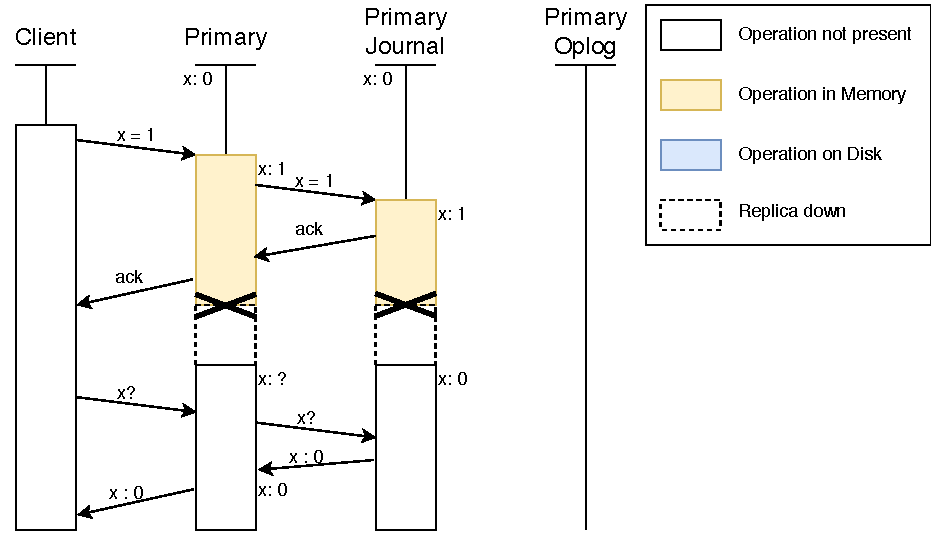
\includegraphics{images/nopersist.pdf}
    \label{fig:nopersist}
    \caption{A time-space diagram of a scenario where a write gets lost due to a failure to persist it on disk}
\end{figure}

This failure relies on two core properties of MongoDB - acknowledging a write before persisting it and only adding a write to the Oplog after flushing it to disk.

Take an operation $o$, with write concern \textit{journaled}, which has just been received by the primary. Currently, the primary stores this operation in memory, performs the operation on the in-memory copy of the data and buffers the write to the journal, but does not yet flush it to disk. Recall that a write is added to the Oplog only \textit{after} it has been flushed to disk. This creates a situation where secondary nodes do not know about a write that has been acknowledged by the primary. As such, if a primary is to crash it will "forget" about $o$ as it was only stored in memory. None of the secondary replicas would have seen $o$ either. A client querying the primary will force it to read the last value of the document operated on from disk. The value returned from the read will not account for the latest operation, which demonstrates the operation has been lost.

Thus, this failure scenario occurs with primary write concern but may also occur with journaled, if the write is buffered instead of being immediately persisted. It will not occur (in a properly implemented MongoDB system) with write concern majority.

\pagebreak
\subsection{Transient Loss via Primary Preferred Read Preference}
\begin{figure}[H]
    \centering
    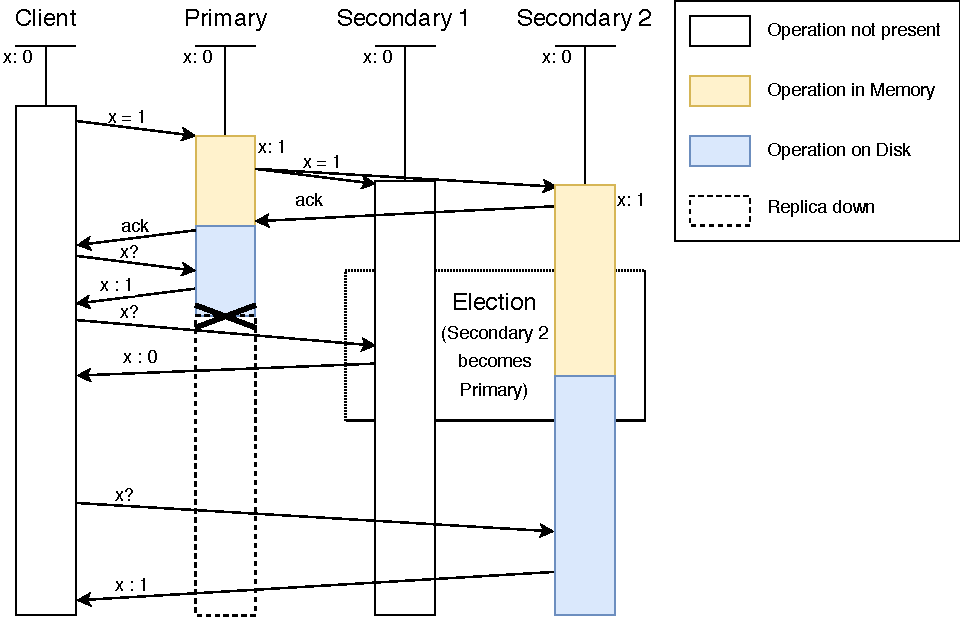
\includegraphics{images/PrimaryPreferred.pdf}
    \label{fig:primarypreferred}
    \caption{A time-space diagram of a scenario where a Majority write concern write gets temporarily lost as a result of the MongoDB client choosing the wrong Secondary to read from.}
\end{figure}

Recall from \prettyref{sec:readpref} that the Primary Preferred read preference will query the secondary if the primary appears to be down, instead of waiting for a primary to respond. The MongoDB client will only query one secondary. This can create a situation where a write will seem to be available, lost and available again. 

Specifically, consider an operation $o$ that was submitted with a majority write concern to the replica set. The primary will acknowledge the write when $\lfloor\frac{|R|}{2}\rfloor$ secondaries also acknowledge the write. This leaves $\lfloor\frac{|R|}{2}\rfloor$ secondaries that may not have acknowledged or even received the write. As such, if the primary is to fail immediately after acknowledging the operation, the MongoDB client has $\frac{\lfloor\frac{|R|}{2}\rfloor - 1}{|R|}$ chance of querying  a secondary that has not seen $o$. Intuitively, this probability reduces with time as more replicas apply the operation to their copy of the data.

If the client is to query the primary, the data returned will have operation $o$ applied to it. Once the primary fails, the MongoDB client has a chance of querying a secondary that has not applied the operation, hence the data returned from that query will not have the operation $o$ applied. Querying the new primary after an election will once again return data with operation $o$ applied. 

As such, Primary Preferred read preference can create instances of transient write loss, where acknowledged operations seem to disappear and reappear during a failure. This scenario can occur in all write concerns, but "all".
\chapter{Experiment Design \& Methodology} \label{chap:experiments}

In this chapter we offer a design and methodology of an experiment and analysis that can quantitatively evaluate the durability of a distributed storage system by measuring the frequency and quantity of write loss under failures. The experiment induces the conditions we identified in \prettyref{chap:det-theory}, and \prettyref{chap:det-results} will report on running the experiments on MongoDB.

\section{Database Contents}

Each document has a simple ID \& value structure as seen in \prettyref{alg:doc}.

\begin{algorithm}
\caption{Example document}
\begin{verbatim}
{
    Id:  5,
    Val: 7
}
\end{verbatim}
\label{alg:doc}
\end{algorithm}

\section{Methodology}

The experiment is set up by creating three identical virtual machines with the database system installed and configured to run in a replica set. We then run a stress test on the replica set using a single client on the host machine which initiates many operations, on separate threads, in parallel. The operations performed are reads, writes and updates on randomly chosen documents with randomly chosen values.

During the run of the experiment, the harness records an execution history, keeping track of each operation performed and error returned by the replica set. Each read, write and update operation is individually recorded into the execution history along with the document id corresponding to the document the operation is performed on,
the timestamp and duration of the operation. Each read record contains the value returned by the database, while the write and update records contain the new value written to the document. Any operations that result in an error are also recorded with the same data.

\begin{figure}
    \begin{CVerbatim}
R,5b9f25ef2644855182a9201c,1042661835,66.689,1537156641143
U,5b9f25ef2644855182a9201c,705768886,1.132,1537156641288
ERR,W,5b9f25f82644855182a92ff2,834995024,22.04,1537156641795
R,5b9f25ef2644855182a9201c,705768886,58.42,1537156641830
    \end{CVerbatim}
    \caption{Sample excerpt of an execution history}
\end{figure}

The experiment is broken into three stages with each stage occupying a third of the experiment time:

\begin{description}
    \item[Standard operation] The virtual machines are started in "Headless" mode and run normally.
    \item[Operating under failure] A failure is induced on the primary. The primary replica disconnects from the replica set initiating an election. 
    \item[Recovery] The failure is reverted and the failed machine is connected back to the replica set.
\end{description}

\section{Failures}

The failures induced during the experiments involve shutting down the primary replica and observing how the secondary nodes behave immediately after the shutdown. The timestamps for when a failure is induced and fixed are also entered into the execution history. 
The following failures are induced in our experiment:

\begin{description}
    \item[Graceful ACPI Shutdown] Sends an ACPI shutdown signal to the virtual machine to trigger a graceful shutdown.
    \item[Hard Poweroff] Simulates an abrupt power failure, which turns the VM off immediately.
\end{description}

Since we focus on crash-tolerant systems, we chose these failures they are supposed to be handled gracefully and correctly by the replica set. This will allow us to find concrete durability failures in the system, that should be possible to prevent within the failure assumptions the system makes. Additionally, they are common system administration scenarios of needing to restart a machine or cutting the power. The recovery flows following these failures will need to re-elect the primary after the failure and, once the failed machine is back up, allow it to "catch up" on the writes which it has not seen.

\section{Workload}
The workload of each experiment consists of three types of operations:

\begin{description}
    \item[Create Document] This operation adds a new document to the collection in the replica set. A new document is created with a value retrieved from a random number generator. Upon acknowledgement of the write from the replica set, its document ID is added to the list of IDs with acknowledged writes.
    \item[Read document] This operation queries the replica set for a document, given its key. The key for the query is chosen randomly from a list of IDs with acknowledged writes. This means, we expect that every query should return a document. Any missing documents are therefore as a result of an error in the replica set.
    \item[Update document] This operation modifies the value of an existing document. The key for the query is chosen randomly from a list of IDs with acknowledged writes and the value is generated using a random number generator.
\end{description}

The primary setting used to vary the workload of the experiment is \textit{write probability}, which determines how often a write operation is issued to the replica set. There are two types of write operations in this experiment - \textit{create document} and \textit{update document}. The decision between which operation to perform is random with equal likelihood.

In addition, we set the Read Concern, Write Concern and Read Preference. This configuration varies between experiments, allowing us to explore the tradeoffs between these configurations and understand which configuration is best for a given scenario.

\section{Execution Analysis}
The execution history produced by each run of the experiment is analysed by Algorithm \ref{alg:eval} to produce the following data:
\begin{description}
    \item[Throughput] The number of successful operations performed during the entire run of the experiment.
    \item[Errors] The number of operations that did not receive a positive acknowledgement, either they got a negative acknowledgement, or they were time out without any acknowledgement.
    \item[Lost Writes] The number of write operations which were lost either temporarily or permanently.
\end{description}

In particular, the algorithm detects when the expected value of the document and value returned from a read are not the same or where the value is missing (denoted by a value of -1). This indicates that a write has either been lost, or that it has been committed but an acknowledgement was not received by the client. We make a distinction between these two cases by keeping track of the write operations that came back as errors to the client which allows us to handle the committed-but-not-acknowledged write and update the state of our analysis as needed. 

\begin{algorithm}
    \caption{Algorithm used for evaluating the execution history}
    \begin{algorithmic}
        \STATE $H \leftarrow$ execution history
        \STATE $t_{fail} \leftarrow$ timestamp of failure induction
        \STATE $t_{fix} \leftarrow$ timestamp of failure repair
        \STATE $D \leftarrow \{\}$ \COMMENT{Lookup of every document's current value}
        \STATE $D_e \leftarrow \{\}$ \COMMENT{Lookup of every write that errored for a document}
        \STATE $E \leftarrow \{\}$ \COMMENT{Set of all errors produced}
        \STATE $M \leftarrow \{\}$ \COMMENT{Set of missing writes}
        \STATE $U \leftarrow \{\}$ \COMMENT{Set of unacknowledged writes}
        \STATE $o \leftarrow 0$ \COMMENT{Number of successful operations}
        \STATE $s \leftarrow $ Normal \COMMENT{Current state of the history (Normal, Failure or Recovery)}

        \FORALL{$h \in H$}
            \IF{$h.time \leq t_{fail}$}
                \STATE $s \leftarrow$ Normal
            \ELSIF{$t_{fail} < h.time \leq t_{fix}$}
                \STATE $s \leftarrow$ Failure
            \ELSE
                \STATE $s \leftarrow$ Recovery
            \ENDIF

            \IF{$h.op =$ Write \OR $h.op =$ Update}
                \STATE $o \leftarrow o+1$
                \STATE $D[h.id] \leftarrow h.val$
            \ELSIF{$h.op =$ Read}
                \STATE $o \leftarrow o+1$
                \IF{$h.val \neq D[h.id]$}
                    \IF{$h.id \in D_e$ \AND $h.val \in D_e[h.id]$}
                        \STATE $U \leftarrow U \cup \{(h.id, h.val, s)\}$
                        \STATE $D[h.id] \leftarrow h.val$
                        \STATE delete $h.val$ from $D_e[h.id]$
                    \ELSE
                        \STATE $M \leftarrow M \cup \{(h.id, h.val, state)\}$
                    \ENDIF
                \ENDIF
            \ELSIF{$h.op =$ Induce}
                \STATE $ s \leftarrow $ Failure
            \ELSIF{$h.op =$ Recover} 
                \STATE $ s \leftarrow $ Recovery
            \ELSIF{$h.op =$ Error}
                \STATE $E \leftarrow E \cup \{(h.err\_op, h.id, h.val, s)\}$
                \IF{$h.err\_op =$ Write \OR $h.err\_op =$ Read}
                    \STATE $D_e[h.id] \leftarrow D_e[h.id] \cup \{h.val\}$
                \ENDIF
            \ENDIF
        \ENDFOR
    \end{algorithmic}
    \label{alg:eval}
\end{algorithm}

Additionally, we also use the execution history to plot the number of different measures against the time of the experiment, bucketed using bins of 1 second.
\chapter{Results} \label{chap:kdur-results}

In this chapter, we present an empirical exploration of time-till-1-durability in MongoDB based on the theory developed in \prettyref{chap:kdur-theory} and proceed to evaluate the results in light of how MongoDB handles write operations.

\section{Environment}
The experiments were performed on the same harness as the one developed in \prettyref{chap:det-results}, using the \textit{Local} read concern and \textit{Primary} read preference. The harness was configured to \textit{not} induce a failure and perform only write operations (using write probability 1). 

\section{Estimating 1-durability}
We ran two experiments, each for 5 minutes. One with write concern \textit{w:1} and one with \textit{journaled}. The execution histories were processed to count the latencies of each operation. The raw results of this collection can be seen in \prettyref{fig:latencies}.

Given that there is a significant difference between the patterns of \textit{w:1} and \textit{journaled} histories, we use the journaled history and apply equation \prettyref{eq:persist} on every operation to derive the time a write becomes 1-durable. Given that VirtualBox networking is very stable, we subtract the average ping latency to the primary from every operation to determine the time that operation became 1-durable. A comparison between 1-durability and \textit{w:1} write acknowledgement can be found in \prettyref{fig:cdf}.

To further clarify the differences between \textit{w:1} and 1-durability, we present a chart of the difference between the two cumulative plots in \prettyref{fig:diff}.

\begin{figure}
    \centering        
    %% Creator: Matplotlib, PGF backend
%%
%% To include the figure in your LaTeX document, write
%%   \input{<filename>.pgf}
%%
%% Make sure the required packages are loaded in your preamble
%%   \usepackage{pgf}
%%
%% Figures using additional raster images can only be included by \input if
%% they are in the same directory as the main LaTeX file. For loading figures
%% from other directories you can use the `import` package
%%   \usepackage{import}
%% and then include the figures with
%%   \import{<path to file>}{<filename>.pgf}
%%
%% Matplotlib used the following preamble
%%   \usepackage[utf8x]{inputenc}
%%   \usepackage[T1]{fontenc}
%%   \usepackage{lmodern}
%%
\begingroup%
\makeatletter%
\begin{pgfpicture}%
\pgfpathrectangle{\pgfpointorigin}{\pgfqpoint{6.400000in}{4.800000in}}%
\pgfusepath{use as bounding box, clip}%
\begin{pgfscope}%
\pgfsetbuttcap%
\pgfsetmiterjoin%
\definecolor{currentfill}{rgb}{1.000000,1.000000,1.000000}%
\pgfsetfillcolor{currentfill}%
\pgfsetlinewidth{0.000000pt}%
\definecolor{currentstroke}{rgb}{1.000000,1.000000,1.000000}%
\pgfsetstrokecolor{currentstroke}%
\pgfsetdash{}{0pt}%
\pgfpathmoveto{\pgfqpoint{0.000000in}{0.000000in}}%
\pgfpathlineto{\pgfqpoint{6.400000in}{0.000000in}}%
\pgfpathlineto{\pgfqpoint{6.400000in}{4.800000in}}%
\pgfpathlineto{\pgfqpoint{0.000000in}{4.800000in}}%
\pgfpathclose%
\pgfusepath{fill}%
\end{pgfscope}%
\begin{pgfscope}%
\pgfsetbuttcap%
\pgfsetmiterjoin%
\definecolor{currentfill}{rgb}{1.000000,1.000000,1.000000}%
\pgfsetfillcolor{currentfill}%
\pgfsetlinewidth{0.000000pt}%
\definecolor{currentstroke}{rgb}{0.000000,0.000000,0.000000}%
\pgfsetstrokecolor{currentstroke}%
\pgfsetstrokeopacity{0.000000}%
\pgfsetdash{}{0pt}%
\pgfpathmoveto{\pgfqpoint{0.800000in}{0.528000in}}%
\pgfpathlineto{\pgfqpoint{5.760000in}{0.528000in}}%
\pgfpathlineto{\pgfqpoint{5.760000in}{4.224000in}}%
\pgfpathlineto{\pgfqpoint{0.800000in}{4.224000in}}%
\pgfpathclose%
\pgfusepath{fill}%
\end{pgfscope}%
\begin{pgfscope}%
\pgfsetbuttcap%
\pgfsetroundjoin%
\definecolor{currentfill}{rgb}{0.000000,0.000000,0.000000}%
\pgfsetfillcolor{currentfill}%
\pgfsetlinewidth{0.803000pt}%
\definecolor{currentstroke}{rgb}{0.000000,0.000000,0.000000}%
\pgfsetstrokecolor{currentstroke}%
\pgfsetdash{}{0pt}%
\pgfsys@defobject{currentmarker}{\pgfqpoint{0.000000in}{-0.048611in}}{\pgfqpoint{0.000000in}{0.000000in}}{%
\pgfpathmoveto{\pgfqpoint{0.000000in}{0.000000in}}%
\pgfpathlineto{\pgfqpoint{0.000000in}{-0.048611in}}%
\pgfusepath{stroke,fill}%
}%
\begin{pgfscope}%
\pgfsys@transformshift{1.020936in}{0.528000in}%
\pgfsys@useobject{currentmarker}{}%
\end{pgfscope}%
\end{pgfscope}%
\begin{pgfscope}%
\pgftext[x=1.020936in,y=0.430778in,,top]{\fontsize{11.000000}{13.200000}\selectfont \(\displaystyle 0\)}%
\end{pgfscope}%
\begin{pgfscope}%
\pgfsetbuttcap%
\pgfsetroundjoin%
\definecolor{currentfill}{rgb}{0.000000,0.000000,0.000000}%
\pgfsetfillcolor{currentfill}%
\pgfsetlinewidth{0.803000pt}%
\definecolor{currentstroke}{rgb}{0.000000,0.000000,0.000000}%
\pgfsetstrokecolor{currentstroke}%
\pgfsetdash{}{0pt}%
\pgfsys@defobject{currentmarker}{\pgfqpoint{0.000000in}{-0.048611in}}{\pgfqpoint{0.000000in}{0.000000in}}{%
\pgfpathmoveto{\pgfqpoint{0.000000in}{0.000000in}}%
\pgfpathlineto{\pgfqpoint{0.000000in}{-0.048611in}}%
\pgfusepath{stroke,fill}%
}%
\begin{pgfscope}%
\pgfsys@transformshift{1.924562in}{0.528000in}%
\pgfsys@useobject{currentmarker}{}%
\end{pgfscope}%
\end{pgfscope}%
\begin{pgfscope}%
\pgftext[x=1.924562in,y=0.430778in,,top]{\fontsize{11.000000}{13.200000}\selectfont \(\displaystyle 200\)}%
\end{pgfscope}%
\begin{pgfscope}%
\pgfsetbuttcap%
\pgfsetroundjoin%
\definecolor{currentfill}{rgb}{0.000000,0.000000,0.000000}%
\pgfsetfillcolor{currentfill}%
\pgfsetlinewidth{0.803000pt}%
\definecolor{currentstroke}{rgb}{0.000000,0.000000,0.000000}%
\pgfsetstrokecolor{currentstroke}%
\pgfsetdash{}{0pt}%
\pgfsys@defobject{currentmarker}{\pgfqpoint{0.000000in}{-0.048611in}}{\pgfqpoint{0.000000in}{0.000000in}}{%
\pgfpathmoveto{\pgfqpoint{0.000000in}{0.000000in}}%
\pgfpathlineto{\pgfqpoint{0.000000in}{-0.048611in}}%
\pgfusepath{stroke,fill}%
}%
\begin{pgfscope}%
\pgfsys@transformshift{2.828187in}{0.528000in}%
\pgfsys@useobject{currentmarker}{}%
\end{pgfscope}%
\end{pgfscope}%
\begin{pgfscope}%
\pgftext[x=2.828187in,y=0.430778in,,top]{\fontsize{11.000000}{13.200000}\selectfont \(\displaystyle 400\)}%
\end{pgfscope}%
\begin{pgfscope}%
\pgfsetbuttcap%
\pgfsetroundjoin%
\definecolor{currentfill}{rgb}{0.000000,0.000000,0.000000}%
\pgfsetfillcolor{currentfill}%
\pgfsetlinewidth{0.803000pt}%
\definecolor{currentstroke}{rgb}{0.000000,0.000000,0.000000}%
\pgfsetstrokecolor{currentstroke}%
\pgfsetdash{}{0pt}%
\pgfsys@defobject{currentmarker}{\pgfqpoint{0.000000in}{-0.048611in}}{\pgfqpoint{0.000000in}{0.000000in}}{%
\pgfpathmoveto{\pgfqpoint{0.000000in}{0.000000in}}%
\pgfpathlineto{\pgfqpoint{0.000000in}{-0.048611in}}%
\pgfusepath{stroke,fill}%
}%
\begin{pgfscope}%
\pgfsys@transformshift{3.731813in}{0.528000in}%
\pgfsys@useobject{currentmarker}{}%
\end{pgfscope}%
\end{pgfscope}%
\begin{pgfscope}%
\pgftext[x=3.731813in,y=0.430778in,,top]{\fontsize{11.000000}{13.200000}\selectfont \(\displaystyle 600\)}%
\end{pgfscope}%
\begin{pgfscope}%
\pgfsetbuttcap%
\pgfsetroundjoin%
\definecolor{currentfill}{rgb}{0.000000,0.000000,0.000000}%
\pgfsetfillcolor{currentfill}%
\pgfsetlinewidth{0.803000pt}%
\definecolor{currentstroke}{rgb}{0.000000,0.000000,0.000000}%
\pgfsetstrokecolor{currentstroke}%
\pgfsetdash{}{0pt}%
\pgfsys@defobject{currentmarker}{\pgfqpoint{0.000000in}{-0.048611in}}{\pgfqpoint{0.000000in}{0.000000in}}{%
\pgfpathmoveto{\pgfqpoint{0.000000in}{0.000000in}}%
\pgfpathlineto{\pgfqpoint{0.000000in}{-0.048611in}}%
\pgfusepath{stroke,fill}%
}%
\begin{pgfscope}%
\pgfsys@transformshift{4.635438in}{0.528000in}%
\pgfsys@useobject{currentmarker}{}%
\end{pgfscope}%
\end{pgfscope}%
\begin{pgfscope}%
\pgftext[x=4.635438in,y=0.430778in,,top]{\fontsize{11.000000}{13.200000}\selectfont \(\displaystyle 800\)}%
\end{pgfscope}%
\begin{pgfscope}%
\pgfsetbuttcap%
\pgfsetroundjoin%
\definecolor{currentfill}{rgb}{0.000000,0.000000,0.000000}%
\pgfsetfillcolor{currentfill}%
\pgfsetlinewidth{0.803000pt}%
\definecolor{currentstroke}{rgb}{0.000000,0.000000,0.000000}%
\pgfsetstrokecolor{currentstroke}%
\pgfsetdash{}{0pt}%
\pgfsys@defobject{currentmarker}{\pgfqpoint{0.000000in}{-0.048611in}}{\pgfqpoint{0.000000in}{0.000000in}}{%
\pgfpathmoveto{\pgfqpoint{0.000000in}{0.000000in}}%
\pgfpathlineto{\pgfqpoint{0.000000in}{-0.048611in}}%
\pgfusepath{stroke,fill}%
}%
\begin{pgfscope}%
\pgfsys@transformshift{5.539064in}{0.528000in}%
\pgfsys@useobject{currentmarker}{}%
\end{pgfscope}%
\end{pgfscope}%
\begin{pgfscope}%
\pgftext[x=5.539064in,y=0.430778in,,top]{\fontsize{11.000000}{13.200000}\selectfont \(\displaystyle 1000\)}%
\end{pgfscope}%
\begin{pgfscope}%
\pgftext[x=3.280000in,y=0.240271in,,top]{\fontsize{11.000000}{13.200000}\selectfont Latency (in milliseconds)}%
\end{pgfscope}%
\begin{pgfscope}%
\pgfsetbuttcap%
\pgfsetroundjoin%
\definecolor{currentfill}{rgb}{0.000000,0.000000,0.000000}%
\pgfsetfillcolor{currentfill}%
\pgfsetlinewidth{0.803000pt}%
\definecolor{currentstroke}{rgb}{0.000000,0.000000,0.000000}%
\pgfsetstrokecolor{currentstroke}%
\pgfsetdash{}{0pt}%
\pgfsys@defobject{currentmarker}{\pgfqpoint{-0.048611in}{0.000000in}}{\pgfqpoint{0.000000in}{0.000000in}}{%
\pgfpathmoveto{\pgfqpoint{0.000000in}{0.000000in}}%
\pgfpathlineto{\pgfqpoint{-0.048611in}{0.000000in}}%
\pgfusepath{stroke,fill}%
}%
\begin{pgfscope}%
\pgfsys@transformshift{0.800000in}{0.696000in}%
\pgfsys@useobject{currentmarker}{}%
\end{pgfscope}%
\end{pgfscope}%
\begin{pgfscope}%
\pgftext[x=0.627981in,y=0.643378in,left,base]{\fontsize{11.000000}{13.200000}\selectfont \(\displaystyle 0\)}%
\end{pgfscope}%
\begin{pgfscope}%
\pgfsetbuttcap%
\pgfsetroundjoin%
\definecolor{currentfill}{rgb}{0.000000,0.000000,0.000000}%
\pgfsetfillcolor{currentfill}%
\pgfsetlinewidth{0.803000pt}%
\definecolor{currentstroke}{rgb}{0.000000,0.000000,0.000000}%
\pgfsetstrokecolor{currentstroke}%
\pgfsetdash{}{0pt}%
\pgfsys@defobject{currentmarker}{\pgfqpoint{-0.048611in}{0.000000in}}{\pgfqpoint{0.000000in}{0.000000in}}{%
\pgfpathmoveto{\pgfqpoint{0.000000in}{0.000000in}}%
\pgfpathlineto{\pgfqpoint{-0.048611in}{0.000000in}}%
\pgfusepath{stroke,fill}%
}%
\begin{pgfscope}%
\pgfsys@transformshift{0.800000in}{1.129492in}%
\pgfsys@useobject{currentmarker}{}%
\end{pgfscope}%
\end{pgfscope}%
\begin{pgfscope}%
\pgftext[x=0.403588in,y=1.076870in,left,base]{\fontsize{11.000000}{13.200000}\selectfont \(\displaystyle 1000\)}%
\end{pgfscope}%
\begin{pgfscope}%
\pgfsetbuttcap%
\pgfsetroundjoin%
\definecolor{currentfill}{rgb}{0.000000,0.000000,0.000000}%
\pgfsetfillcolor{currentfill}%
\pgfsetlinewidth{0.803000pt}%
\definecolor{currentstroke}{rgb}{0.000000,0.000000,0.000000}%
\pgfsetstrokecolor{currentstroke}%
\pgfsetdash{}{0pt}%
\pgfsys@defobject{currentmarker}{\pgfqpoint{-0.048611in}{0.000000in}}{\pgfqpoint{0.000000in}{0.000000in}}{%
\pgfpathmoveto{\pgfqpoint{0.000000in}{0.000000in}}%
\pgfpathlineto{\pgfqpoint{-0.048611in}{0.000000in}}%
\pgfusepath{stroke,fill}%
}%
\begin{pgfscope}%
\pgfsys@transformshift{0.800000in}{1.562985in}%
\pgfsys@useobject{currentmarker}{}%
\end{pgfscope}%
\end{pgfscope}%
\begin{pgfscope}%
\pgftext[x=0.403588in,y=1.510363in,left,base]{\fontsize{11.000000}{13.200000}\selectfont \(\displaystyle 2000\)}%
\end{pgfscope}%
\begin{pgfscope}%
\pgfsetbuttcap%
\pgfsetroundjoin%
\definecolor{currentfill}{rgb}{0.000000,0.000000,0.000000}%
\pgfsetfillcolor{currentfill}%
\pgfsetlinewidth{0.803000pt}%
\definecolor{currentstroke}{rgb}{0.000000,0.000000,0.000000}%
\pgfsetstrokecolor{currentstroke}%
\pgfsetdash{}{0pt}%
\pgfsys@defobject{currentmarker}{\pgfqpoint{-0.048611in}{0.000000in}}{\pgfqpoint{0.000000in}{0.000000in}}{%
\pgfpathmoveto{\pgfqpoint{0.000000in}{0.000000in}}%
\pgfpathlineto{\pgfqpoint{-0.048611in}{0.000000in}}%
\pgfusepath{stroke,fill}%
}%
\begin{pgfscope}%
\pgfsys@transformshift{0.800000in}{1.996477in}%
\pgfsys@useobject{currentmarker}{}%
\end{pgfscope}%
\end{pgfscope}%
\begin{pgfscope}%
\pgftext[x=0.403588in,y=1.943855in,left,base]{\fontsize{11.000000}{13.200000}\selectfont \(\displaystyle 3000\)}%
\end{pgfscope}%
\begin{pgfscope}%
\pgfsetbuttcap%
\pgfsetroundjoin%
\definecolor{currentfill}{rgb}{0.000000,0.000000,0.000000}%
\pgfsetfillcolor{currentfill}%
\pgfsetlinewidth{0.803000pt}%
\definecolor{currentstroke}{rgb}{0.000000,0.000000,0.000000}%
\pgfsetstrokecolor{currentstroke}%
\pgfsetdash{}{0pt}%
\pgfsys@defobject{currentmarker}{\pgfqpoint{-0.048611in}{0.000000in}}{\pgfqpoint{0.000000in}{0.000000in}}{%
\pgfpathmoveto{\pgfqpoint{0.000000in}{0.000000in}}%
\pgfpathlineto{\pgfqpoint{-0.048611in}{0.000000in}}%
\pgfusepath{stroke,fill}%
}%
\begin{pgfscope}%
\pgfsys@transformshift{0.800000in}{2.429970in}%
\pgfsys@useobject{currentmarker}{}%
\end{pgfscope}%
\end{pgfscope}%
\begin{pgfscope}%
\pgftext[x=0.403588in,y=2.377348in,left,base]{\fontsize{11.000000}{13.200000}\selectfont \(\displaystyle 4000\)}%
\end{pgfscope}%
\begin{pgfscope}%
\pgfsetbuttcap%
\pgfsetroundjoin%
\definecolor{currentfill}{rgb}{0.000000,0.000000,0.000000}%
\pgfsetfillcolor{currentfill}%
\pgfsetlinewidth{0.803000pt}%
\definecolor{currentstroke}{rgb}{0.000000,0.000000,0.000000}%
\pgfsetstrokecolor{currentstroke}%
\pgfsetdash{}{0pt}%
\pgfsys@defobject{currentmarker}{\pgfqpoint{-0.048611in}{0.000000in}}{\pgfqpoint{0.000000in}{0.000000in}}{%
\pgfpathmoveto{\pgfqpoint{0.000000in}{0.000000in}}%
\pgfpathlineto{\pgfqpoint{-0.048611in}{0.000000in}}%
\pgfusepath{stroke,fill}%
}%
\begin{pgfscope}%
\pgfsys@transformshift{0.800000in}{2.863462in}%
\pgfsys@useobject{currentmarker}{}%
\end{pgfscope}%
\end{pgfscope}%
\begin{pgfscope}%
\pgftext[x=0.403588in,y=2.810840in,left,base]{\fontsize{11.000000}{13.200000}\selectfont \(\displaystyle 5000\)}%
\end{pgfscope}%
\begin{pgfscope}%
\pgfsetbuttcap%
\pgfsetroundjoin%
\definecolor{currentfill}{rgb}{0.000000,0.000000,0.000000}%
\pgfsetfillcolor{currentfill}%
\pgfsetlinewidth{0.803000pt}%
\definecolor{currentstroke}{rgb}{0.000000,0.000000,0.000000}%
\pgfsetstrokecolor{currentstroke}%
\pgfsetdash{}{0pt}%
\pgfsys@defobject{currentmarker}{\pgfqpoint{-0.048611in}{0.000000in}}{\pgfqpoint{0.000000in}{0.000000in}}{%
\pgfpathmoveto{\pgfqpoint{0.000000in}{0.000000in}}%
\pgfpathlineto{\pgfqpoint{-0.048611in}{0.000000in}}%
\pgfusepath{stroke,fill}%
}%
\begin{pgfscope}%
\pgfsys@transformshift{0.800000in}{3.296955in}%
\pgfsys@useobject{currentmarker}{}%
\end{pgfscope}%
\end{pgfscope}%
\begin{pgfscope}%
\pgftext[x=0.403588in,y=3.244332in,left,base]{\fontsize{11.000000}{13.200000}\selectfont \(\displaystyle 6000\)}%
\end{pgfscope}%
\begin{pgfscope}%
\pgfsetbuttcap%
\pgfsetroundjoin%
\definecolor{currentfill}{rgb}{0.000000,0.000000,0.000000}%
\pgfsetfillcolor{currentfill}%
\pgfsetlinewidth{0.803000pt}%
\definecolor{currentstroke}{rgb}{0.000000,0.000000,0.000000}%
\pgfsetstrokecolor{currentstroke}%
\pgfsetdash{}{0pt}%
\pgfsys@defobject{currentmarker}{\pgfqpoint{-0.048611in}{0.000000in}}{\pgfqpoint{0.000000in}{0.000000in}}{%
\pgfpathmoveto{\pgfqpoint{0.000000in}{0.000000in}}%
\pgfpathlineto{\pgfqpoint{-0.048611in}{0.000000in}}%
\pgfusepath{stroke,fill}%
}%
\begin{pgfscope}%
\pgfsys@transformshift{0.800000in}{3.730447in}%
\pgfsys@useobject{currentmarker}{}%
\end{pgfscope}%
\end{pgfscope}%
\begin{pgfscope}%
\pgftext[x=0.403588in,y=3.677825in,left,base]{\fontsize{11.000000}{13.200000}\selectfont \(\displaystyle 7000\)}%
\end{pgfscope}%
\begin{pgfscope}%
\pgfsetbuttcap%
\pgfsetroundjoin%
\definecolor{currentfill}{rgb}{0.000000,0.000000,0.000000}%
\pgfsetfillcolor{currentfill}%
\pgfsetlinewidth{0.803000pt}%
\definecolor{currentstroke}{rgb}{0.000000,0.000000,0.000000}%
\pgfsetstrokecolor{currentstroke}%
\pgfsetdash{}{0pt}%
\pgfsys@defobject{currentmarker}{\pgfqpoint{-0.048611in}{0.000000in}}{\pgfqpoint{0.000000in}{0.000000in}}{%
\pgfpathmoveto{\pgfqpoint{0.000000in}{0.000000in}}%
\pgfpathlineto{\pgfqpoint{-0.048611in}{0.000000in}}%
\pgfusepath{stroke,fill}%
}%
\begin{pgfscope}%
\pgfsys@transformshift{0.800000in}{4.163940in}%
\pgfsys@useobject{currentmarker}{}%
\end{pgfscope}%
\end{pgfscope}%
\begin{pgfscope}%
\pgftext[x=0.403588in,y=4.111317in,left,base]{\fontsize{11.000000}{13.200000}\selectfont \(\displaystyle 8000\)}%
\end{pgfscope}%
\begin{pgfscope}%
\pgftext[x=0.348033in,y=2.376000in,,bottom,rotate=90.000000]{\fontsize{11.000000}{13.200000}\selectfont Number of operations}%
\end{pgfscope}%
\begin{pgfscope}%
\pgfpathrectangle{\pgfqpoint{0.800000in}{0.528000in}}{\pgfqpoint{4.960000in}{3.696000in}}%
\pgfusepath{clip}%
\pgfsetrectcap%
\pgfsetroundjoin%
\pgfsetlinewidth{1.505625pt}%
\definecolor{currentstroke}{rgb}{0.121569,0.466667,0.705882}%
\pgfsetstrokecolor{currentstroke}%
\pgfsetdash{}{0pt}%
\pgfpathmoveto{\pgfqpoint{1.025455in}{1.752855in}}%
\pgfpathlineto{\pgfqpoint{1.029973in}{1.641447in}}%
\pgfpathlineto{\pgfqpoint{1.034491in}{1.632344in}}%
\pgfpathlineto{\pgfqpoint{1.039009in}{1.615871in}}%
\pgfpathlineto{\pgfqpoint{1.043527in}{1.570788in}}%
\pgfpathlineto{\pgfqpoint{1.048045in}{1.623674in}}%
\pgfpathlineto{\pgfqpoint{1.052563in}{1.613270in}}%
\pgfpathlineto{\pgfqpoint{1.061600in}{1.502296in}}%
\pgfpathlineto{\pgfqpoint{1.066118in}{1.454178in}}%
\pgfpathlineto{\pgfqpoint{1.070636in}{1.436839in}}%
\pgfpathlineto{\pgfqpoint{1.075154in}{1.357943in}}%
\pgfpathlineto{\pgfqpoint{1.079672in}{1.379184in}}%
\pgfpathlineto{\pgfqpoint{1.084190in}{1.332367in}}%
\pgfpathlineto{\pgfqpoint{1.097745in}{1.240467in}}%
\pgfpathlineto{\pgfqpoint{1.102263in}{1.184979in}}%
\pgfpathlineto{\pgfqpoint{1.106781in}{1.148133in}}%
\pgfpathlineto{\pgfqpoint{1.111299in}{1.142064in}}%
\pgfpathlineto{\pgfqpoint{1.115817in}{1.080941in}}%
\pgfpathlineto{\pgfqpoint{1.120335in}{1.077473in}}%
\pgfpathlineto{\pgfqpoint{1.124853in}{1.051897in}}%
\pgfpathlineto{\pgfqpoint{1.129371in}{1.044961in}}%
\pgfpathlineto{\pgfqpoint{1.133890in}{1.019819in}}%
\pgfpathlineto{\pgfqpoint{1.138408in}{1.002479in}}%
\pgfpathlineto{\pgfqpoint{1.147444in}{0.945692in}}%
\pgfpathlineto{\pgfqpoint{1.151962in}{0.924451in}}%
\pgfpathlineto{\pgfqpoint{1.156480in}{0.941790in}}%
\pgfpathlineto{\pgfqpoint{1.160998in}{0.890638in}}%
\pgfpathlineto{\pgfqpoint{1.165516in}{0.902342in}}%
\pgfpathlineto{\pgfqpoint{1.174553in}{0.842087in}}%
\pgfpathlineto{\pgfqpoint{1.179071in}{0.838186in}}%
\pgfpathlineto{\pgfqpoint{1.183589in}{0.841220in}}%
\pgfpathlineto{\pgfqpoint{1.188107in}{0.829082in}}%
\pgfpathlineto{\pgfqpoint{1.192625in}{0.837752in}}%
\pgfpathlineto{\pgfqpoint{1.197143in}{0.825181in}}%
\pgfpathlineto{\pgfqpoint{1.201662in}{0.835151in}}%
\pgfpathlineto{\pgfqpoint{1.206180in}{0.827782in}}%
\pgfpathlineto{\pgfqpoint{1.210698in}{0.845988in}}%
\pgfpathlineto{\pgfqpoint{1.215216in}{0.857693in}}%
\pgfpathlineto{\pgfqpoint{1.219734in}{0.886303in}}%
\pgfpathlineto{\pgfqpoint{1.224252in}{0.924451in}}%
\pgfpathlineto{\pgfqpoint{1.228770in}{0.944825in}}%
\pgfpathlineto{\pgfqpoint{1.237807in}{1.063602in}}%
\pgfpathlineto{\pgfqpoint{1.242325in}{1.126025in}}%
\pgfpathlineto{\pgfqpoint{1.246843in}{1.347973in}}%
\pgfpathlineto{\pgfqpoint{1.251361in}{1.315461in}}%
\pgfpathlineto{\pgfqpoint{1.255879in}{1.435105in}}%
\pgfpathlineto{\pgfqpoint{1.260397in}{1.496661in}}%
\pgfpathlineto{\pgfqpoint{1.264915in}{1.742884in}}%
\pgfpathlineto{\pgfqpoint{1.273952in}{2.383153in}}%
\pgfpathlineto{\pgfqpoint{1.278470in}{2.811877in}}%
\pgfpathlineto{\pgfqpoint{1.282988in}{2.925018in}}%
\pgfpathlineto{\pgfqpoint{1.287506in}{2.944959in}}%
\pgfpathlineto{\pgfqpoint{1.292024in}{3.285684in}}%
\pgfpathlineto{\pgfqpoint{1.296542in}{3.500696in}}%
\pgfpathlineto{\pgfqpoint{1.301060in}{3.795471in}}%
\pgfpathlineto{\pgfqpoint{1.305578in}{3.819747in}}%
\pgfpathlineto{\pgfqpoint{1.310097in}{3.826249in}}%
\pgfpathlineto{\pgfqpoint{1.314615in}{4.056000in}}%
\pgfpathlineto{\pgfqpoint{1.319133in}{3.809343in}}%
\pgfpathlineto{\pgfqpoint{1.323651in}{3.720477in}}%
\pgfpathlineto{\pgfqpoint{1.328169in}{3.785934in}}%
\pgfpathlineto{\pgfqpoint{1.332687in}{3.953262in}}%
\pgfpathlineto{\pgfqpoint{1.337205in}{4.017853in}}%
\pgfpathlineto{\pgfqpoint{1.341723in}{4.033458in}}%
\pgfpathlineto{\pgfqpoint{1.346242in}{3.977104in}}%
\pgfpathlineto{\pgfqpoint{1.355278in}{3.625975in}}%
\pgfpathlineto{\pgfqpoint{1.359796in}{3.322097in}}%
\pgfpathlineto{\pgfqpoint{1.364314in}{3.151735in}}%
\pgfpathlineto{\pgfqpoint{1.368832in}{2.882969in}}%
\pgfpathlineto{\pgfqpoint{1.391423in}{2.148200in}}%
\pgfpathlineto{\pgfqpoint{1.400459in}{1.983906in}}%
\pgfpathlineto{\pgfqpoint{1.404977in}{1.849957in}}%
\pgfpathlineto{\pgfqpoint{1.414013in}{1.676993in}}%
\pgfpathlineto{\pgfqpoint{1.423050in}{1.565152in}}%
\pgfpathlineto{\pgfqpoint{1.427568in}{1.466316in}}%
\pgfpathlineto{\pgfqpoint{1.432086in}{1.421666in}}%
\pgfpathlineto{\pgfqpoint{1.436604in}{1.327599in}}%
\pgfpathlineto{\pgfqpoint{1.441122in}{1.269077in}}%
\pgfpathlineto{\pgfqpoint{1.445640in}{1.277747in}}%
\pgfpathlineto{\pgfqpoint{1.450158in}{1.276013in}}%
\pgfpathlineto{\pgfqpoint{1.454677in}{1.243067in}}%
\pgfpathlineto{\pgfqpoint{1.459195in}{1.229629in}}%
\pgfpathlineto{\pgfqpoint{1.463713in}{1.184979in}}%
\pgfpathlineto{\pgfqpoint{1.468231in}{1.108251in}}%
\pgfpathlineto{\pgfqpoint{1.472749in}{1.091345in}}%
\pgfpathlineto{\pgfqpoint{1.477267in}{1.093513in}}%
\pgfpathlineto{\pgfqpoint{1.481785in}{1.081375in}}%
\pgfpathlineto{\pgfqpoint{1.490822in}{0.973435in}}%
\pgfpathlineto{\pgfqpoint{1.495340in}{0.980371in}}%
\pgfpathlineto{\pgfqpoint{1.499858in}{1.012016in}}%
\pgfpathlineto{\pgfqpoint{1.504376in}{0.963898in}}%
\pgfpathlineto{\pgfqpoint{1.508894in}{0.977337in}}%
\pgfpathlineto{\pgfqpoint{1.513412in}{1.004647in}}%
\pgfpathlineto{\pgfqpoint{1.517930in}{1.020252in}}%
\pgfpathlineto{\pgfqpoint{1.522449in}{1.025454in}}%
\pgfpathlineto{\pgfqpoint{1.526967in}{1.078774in}}%
\pgfpathlineto{\pgfqpoint{1.531485in}{1.110852in}}%
\pgfpathlineto{\pgfqpoint{1.536003in}{1.189748in}}%
\pgfpathlineto{\pgfqpoint{1.540521in}{1.138162in}}%
\pgfpathlineto{\pgfqpoint{1.545039in}{1.237432in}}%
\pgfpathlineto{\pgfqpoint{1.554075in}{1.305057in}}%
\pgfpathlineto{\pgfqpoint{1.558594in}{1.378317in}}%
\pgfpathlineto{\pgfqpoint{1.563112in}{1.471951in}}%
\pgfpathlineto{\pgfqpoint{1.567630in}{1.603300in}}%
\pgfpathlineto{\pgfqpoint{1.572148in}{1.550847in}}%
\pgfpathlineto{\pgfqpoint{1.576666in}{1.672658in}}%
\pgfpathlineto{\pgfqpoint{1.581184in}{1.702136in}}%
\pgfpathlineto{\pgfqpoint{1.585702in}{1.791435in}}%
\pgfpathlineto{\pgfqpoint{1.590220in}{1.761091in}}%
\pgfpathlineto{\pgfqpoint{1.599257in}{1.924084in}}%
\pgfpathlineto{\pgfqpoint{1.612811in}{2.146899in}}%
\pgfpathlineto{\pgfqpoint{1.617329in}{2.258307in}}%
\pgfpathlineto{\pgfqpoint{1.621847in}{2.423467in}}%
\pgfpathlineto{\pgfqpoint{1.626365in}{2.496294in}}%
\pgfpathlineto{\pgfqpoint{1.630884in}{2.638480in}}%
\pgfpathlineto{\pgfqpoint{1.635402in}{2.709572in}}%
\pgfpathlineto{\pgfqpoint{1.639920in}{2.857827in}}%
\pgfpathlineto{\pgfqpoint{1.644438in}{2.914181in}}%
\pgfpathlineto{\pgfqpoint{1.648956in}{3.095814in}}%
\pgfpathlineto{\pgfqpoint{1.653474in}{2.964033in}}%
\pgfpathlineto{\pgfqpoint{1.657992in}{3.016485in}}%
\pgfpathlineto{\pgfqpoint{1.662510in}{3.015185in}}%
\pgfpathlineto{\pgfqpoint{1.667029in}{2.932821in}}%
\pgfpathlineto{\pgfqpoint{1.671547in}{2.747286in}}%
\pgfpathlineto{\pgfqpoint{1.676065in}{2.692233in}}%
\pgfpathlineto{\pgfqpoint{1.685101in}{2.489792in}}%
\pgfpathlineto{\pgfqpoint{1.689619in}{2.528373in}}%
\pgfpathlineto{\pgfqpoint{1.694137in}{2.403527in}}%
\pgfpathlineto{\pgfqpoint{1.698655in}{2.352808in}}%
\pgfpathlineto{\pgfqpoint{1.703174in}{2.323764in}}%
\pgfpathlineto{\pgfqpoint{1.707692in}{2.322464in}}%
\pgfpathlineto{\pgfqpoint{1.716728in}{2.035925in}}%
\pgfpathlineto{\pgfqpoint{1.721246in}{2.004280in}}%
\pgfpathlineto{\pgfqpoint{1.725764in}{1.848656in}}%
\pgfpathlineto{\pgfqpoint{1.730282in}{1.737249in}}%
\pgfpathlineto{\pgfqpoint{1.734801in}{1.731180in}}%
\pgfpathlineto{\pgfqpoint{1.739319in}{1.646215in}}%
\pgfpathlineto{\pgfqpoint{1.748355in}{1.534808in}}%
\pgfpathlineto{\pgfqpoint{1.752873in}{1.513133in}}%
\pgfpathlineto{\pgfqpoint{1.757391in}{1.441607in}}%
\pgfpathlineto{\pgfqpoint{1.766427in}{1.376583in}}%
\pgfpathlineto{\pgfqpoint{1.770946in}{1.371815in}}%
\pgfpathlineto{\pgfqpoint{1.775464in}{1.348406in}}%
\pgfpathlineto{\pgfqpoint{1.779982in}{1.292919in}}%
\pgfpathlineto{\pgfqpoint{1.784500in}{1.255205in}}%
\pgfpathlineto{\pgfqpoint{1.789018in}{1.234831in}}%
\pgfpathlineto{\pgfqpoint{1.793536in}{1.250870in}}%
\pgfpathlineto{\pgfqpoint{1.798054in}{1.214890in}}%
\pgfpathlineto{\pgfqpoint{1.802572in}{1.282949in}}%
\pgfpathlineto{\pgfqpoint{1.807091in}{1.157669in}}%
\pgfpathlineto{\pgfqpoint{1.811609in}{1.167206in}}%
\pgfpathlineto{\pgfqpoint{1.820645in}{1.200585in}}%
\pgfpathlineto{\pgfqpoint{1.825163in}{1.212290in}}%
\pgfpathlineto{\pgfqpoint{1.829681in}{1.228762in}}%
\pgfpathlineto{\pgfqpoint{1.834199in}{1.258240in}}%
\pgfpathlineto{\pgfqpoint{1.838717in}{1.209689in}}%
\pgfpathlineto{\pgfqpoint{1.843236in}{1.213156in}}%
\pgfpathlineto{\pgfqpoint{1.847754in}{1.293353in}}%
\pgfpathlineto{\pgfqpoint{1.852272in}{1.214890in}}%
\pgfpathlineto{\pgfqpoint{1.856790in}{1.219225in}}%
\pgfpathlineto{\pgfqpoint{1.861308in}{1.263008in}}%
\pgfpathlineto{\pgfqpoint{1.865826in}{1.239166in}}%
\pgfpathlineto{\pgfqpoint{1.870344in}{1.230063in}}%
\pgfpathlineto{\pgfqpoint{1.874862in}{1.254338in}}%
\pgfpathlineto{\pgfqpoint{1.879381in}{1.372248in}}%
\pgfpathlineto{\pgfqpoint{1.883899in}{1.419499in}}%
\pgfpathlineto{\pgfqpoint{1.888417in}{1.355342in}}%
\pgfpathlineto{\pgfqpoint{1.892935in}{1.405194in}}%
\pgfpathlineto{\pgfqpoint{1.897453in}{1.474552in}}%
\pgfpathlineto{\pgfqpoint{1.901971in}{1.505764in}}%
\pgfpathlineto{\pgfqpoint{1.906489in}{1.510532in}}%
\pgfpathlineto{\pgfqpoint{1.911007in}{1.559950in}}%
\pgfpathlineto{\pgfqpoint{1.915526in}{1.534808in}}%
\pgfpathlineto{\pgfqpoint{1.920044in}{1.527005in}}%
\pgfpathlineto{\pgfqpoint{1.924562in}{1.527872in}}%
\pgfpathlineto{\pgfqpoint{1.929080in}{1.539576in}}%
\pgfpathlineto{\pgfqpoint{1.933598in}{1.578157in}}%
\pgfpathlineto{\pgfqpoint{1.938116in}{1.629743in}}%
\pgfpathlineto{\pgfqpoint{1.942634in}{1.619339in}}%
\pgfpathlineto{\pgfqpoint{1.947152in}{1.644915in}}%
\pgfpathlineto{\pgfqpoint{1.951671in}{1.618905in}}%
\pgfpathlineto{\pgfqpoint{1.956189in}{1.713840in}}%
\pgfpathlineto{\pgfqpoint{1.960707in}{1.715574in}}%
\pgfpathlineto{\pgfqpoint{1.965225in}{1.683929in}}%
\pgfpathlineto{\pgfqpoint{1.969743in}{1.739416in}}%
\pgfpathlineto{\pgfqpoint{1.974261in}{1.658353in}}%
\pgfpathlineto{\pgfqpoint{1.978779in}{1.670925in}}%
\pgfpathlineto{\pgfqpoint{1.983298in}{1.674392in}}%
\pgfpathlineto{\pgfqpoint{1.987816in}{1.630176in}}%
\pgfpathlineto{\pgfqpoint{1.992334in}{1.604600in}}%
\pgfpathlineto{\pgfqpoint{1.996852in}{1.597664in}}%
\pgfpathlineto{\pgfqpoint{2.001370in}{1.546512in}}%
\pgfpathlineto{\pgfqpoint{2.005888in}{1.535675in}}%
\pgfpathlineto{\pgfqpoint{2.010406in}{1.495794in}}%
\pgfpathlineto{\pgfqpoint{2.014924in}{1.471085in}}%
\pgfpathlineto{\pgfqpoint{2.019443in}{1.459814in}}%
\pgfpathlineto{\pgfqpoint{2.023961in}{1.429469in}}%
\pgfpathlineto{\pgfqpoint{2.028479in}{1.416031in}}%
\pgfpathlineto{\pgfqpoint{2.032997in}{1.307224in}}%
\pgfpathlineto{\pgfqpoint{2.037515in}{1.298121in}}%
\pgfpathlineto{\pgfqpoint{2.042033in}{1.270811in}}%
\pgfpathlineto{\pgfqpoint{2.046551in}{1.305057in}}%
\pgfpathlineto{\pgfqpoint{2.055588in}{1.193216in}}%
\pgfpathlineto{\pgfqpoint{2.060106in}{1.197551in}}%
\pgfpathlineto{\pgfqpoint{2.064624in}{1.167640in}}%
\pgfpathlineto{\pgfqpoint{2.069142in}{1.180211in}}%
\pgfpathlineto{\pgfqpoint{2.078178in}{1.181078in}}%
\pgfpathlineto{\pgfqpoint{2.082696in}{1.118222in}}%
\pgfpathlineto{\pgfqpoint{2.087214in}{1.116921in}}%
\pgfpathlineto{\pgfqpoint{2.096251in}{1.060567in}}%
\pgfpathlineto{\pgfqpoint{2.100769in}{1.091345in}}%
\pgfpathlineto{\pgfqpoint{2.105287in}{1.045828in}}%
\pgfpathlineto{\pgfqpoint{2.109805in}{1.063168in}}%
\pgfpathlineto{\pgfqpoint{2.118841in}{1.065769in}}%
\pgfpathlineto{\pgfqpoint{2.123359in}{1.065769in}}%
\pgfpathlineto{\pgfqpoint{2.127878in}{1.069670in}}%
\pgfpathlineto{\pgfqpoint{2.132396in}{1.080508in}}%
\pgfpathlineto{\pgfqpoint{2.136914in}{1.110852in}}%
\pgfpathlineto{\pgfqpoint{2.141432in}{1.132527in}}%
\pgfpathlineto{\pgfqpoint{2.145950in}{1.087877in}}%
\pgfpathlineto{\pgfqpoint{2.150468in}{1.098281in}}%
\pgfpathlineto{\pgfqpoint{2.154986in}{1.043661in}}%
\pgfpathlineto{\pgfqpoint{2.159504in}{1.046262in}}%
\pgfpathlineto{\pgfqpoint{2.164023in}{1.050597in}}%
\pgfpathlineto{\pgfqpoint{2.168541in}{1.042360in}}%
\pgfpathlineto{\pgfqpoint{2.173059in}{1.054065in}}%
\pgfpathlineto{\pgfqpoint{2.177577in}{1.044094in}}%
\pgfpathlineto{\pgfqpoint{2.182095in}{1.062735in}}%
\pgfpathlineto{\pgfqpoint{2.186613in}{1.045828in}}%
\pgfpathlineto{\pgfqpoint{2.191131in}{1.065336in}}%
\pgfpathlineto{\pgfqpoint{2.195649in}{1.025888in}}%
\pgfpathlineto{\pgfqpoint{2.200168in}{1.018518in}}%
\pgfpathlineto{\pgfqpoint{2.209204in}{1.017651in}}%
\pgfpathlineto{\pgfqpoint{2.213722in}{1.010282in}}%
\pgfpathlineto{\pgfqpoint{2.218240in}{0.992509in}}%
\pgfpathlineto{\pgfqpoint{2.222758in}{1.012449in}}%
\pgfpathlineto{\pgfqpoint{2.227276in}{1.044528in}}%
\pgfpathlineto{\pgfqpoint{2.231794in}{1.058833in}}%
\pgfpathlineto{\pgfqpoint{2.236313in}{1.053631in}}%
\pgfpathlineto{\pgfqpoint{2.240831in}{1.053631in}}%
\pgfpathlineto{\pgfqpoint{2.245349in}{1.078340in}}%
\pgfpathlineto{\pgfqpoint{2.249867in}{1.061868in}}%
\pgfpathlineto{\pgfqpoint{2.254385in}{1.104783in}}%
\pgfpathlineto{\pgfqpoint{2.258903in}{1.101315in}}%
\pgfpathlineto{\pgfqpoint{2.263421in}{1.121256in}}%
\pgfpathlineto{\pgfqpoint{2.267940in}{1.091345in}}%
\pgfpathlineto{\pgfqpoint{2.272458in}{1.104350in}}%
\pgfpathlineto{\pgfqpoint{2.276976in}{1.075739in}}%
\pgfpathlineto{\pgfqpoint{2.281494in}{1.073138in}}%
\pgfpathlineto{\pgfqpoint{2.286012in}{1.079641in}}%
\pgfpathlineto{\pgfqpoint{2.290530in}{1.070537in}}%
\pgfpathlineto{\pgfqpoint{2.295048in}{1.037592in}}%
\pgfpathlineto{\pgfqpoint{2.299566in}{1.016351in}}%
\pgfpathlineto{\pgfqpoint{2.304085in}{1.087010in}}%
\pgfpathlineto{\pgfqpoint{2.308603in}{1.055799in}}%
\pgfpathlineto{\pgfqpoint{2.313121in}{1.049296in}}%
\pgfpathlineto{\pgfqpoint{2.317639in}{1.044961in}}%
\pgfpathlineto{\pgfqpoint{2.322157in}{1.050597in}}%
\pgfpathlineto{\pgfqpoint{2.331193in}{0.992509in}}%
\pgfpathlineto{\pgfqpoint{2.335711in}{0.999445in}}%
\pgfpathlineto{\pgfqpoint{2.340230in}{0.978637in}}%
\pgfpathlineto{\pgfqpoint{2.344748in}{0.994676in}}%
\pgfpathlineto{\pgfqpoint{2.353784in}{0.953928in}}%
\pgfpathlineto{\pgfqpoint{2.358302in}{0.948293in}}%
\pgfpathlineto{\pgfqpoint{2.362820in}{1.014617in}}%
\pgfpathlineto{\pgfqpoint{2.367338in}{0.963031in}}%
\pgfpathlineto{\pgfqpoint{2.371856in}{0.946559in}}%
\pgfpathlineto{\pgfqpoint{2.376375in}{0.925751in}}%
\pgfpathlineto{\pgfqpoint{2.380893in}{0.924884in}}%
\pgfpathlineto{\pgfqpoint{2.389929in}{0.917081in}}%
\pgfpathlineto{\pgfqpoint{2.394447in}{0.940923in}}%
\pgfpathlineto{\pgfqpoint{2.398965in}{0.937022in}}%
\pgfpathlineto{\pgfqpoint{2.403483in}{0.937889in}}%
\pgfpathlineto{\pgfqpoint{2.408001in}{0.903209in}}%
\pgfpathlineto{\pgfqpoint{2.412520in}{0.904943in}}%
\pgfpathlineto{\pgfqpoint{2.417038in}{0.909278in}}%
\pgfpathlineto{\pgfqpoint{2.421556in}{0.923150in}}%
\pgfpathlineto{\pgfqpoint{2.426074in}{0.915781in}}%
\pgfpathlineto{\pgfqpoint{2.430592in}{0.949593in}}%
\pgfpathlineto{\pgfqpoint{2.439628in}{0.933987in}}%
\pgfpathlineto{\pgfqpoint{2.444146in}{0.941357in}}%
\pgfpathlineto{\pgfqpoint{2.448665in}{0.920116in}}%
\pgfpathlineto{\pgfqpoint{2.453183in}{0.887604in}}%
\pgfpathlineto{\pgfqpoint{2.457701in}{0.885003in}}%
\pgfpathlineto{\pgfqpoint{2.466737in}{0.915347in}}%
\pgfpathlineto{\pgfqpoint{2.471255in}{0.906677in}}%
\pgfpathlineto{\pgfqpoint{2.475773in}{0.875899in}}%
\pgfpathlineto{\pgfqpoint{2.484810in}{0.877633in}}%
\pgfpathlineto{\pgfqpoint{2.493846in}{0.866363in}}%
\pgfpathlineto{\pgfqpoint{2.498364in}{0.878934in}}%
\pgfpathlineto{\pgfqpoint{2.502882in}{0.871564in}}%
\pgfpathlineto{\pgfqpoint{2.507400in}{0.881101in}}%
\pgfpathlineto{\pgfqpoint{2.511918in}{0.867230in}}%
\pgfpathlineto{\pgfqpoint{2.516437in}{0.889771in}}%
\pgfpathlineto{\pgfqpoint{2.520955in}{0.878934in}}%
\pgfpathlineto{\pgfqpoint{2.525473in}{0.881535in}}%
\pgfpathlineto{\pgfqpoint{2.529991in}{0.880668in}}%
\pgfpathlineto{\pgfqpoint{2.534509in}{0.864629in}}%
\pgfpathlineto{\pgfqpoint{2.539027in}{0.874599in}}%
\pgfpathlineto{\pgfqpoint{2.543545in}{0.860727in}}%
\pgfpathlineto{\pgfqpoint{2.548063in}{0.868963in}}%
\pgfpathlineto{\pgfqpoint{2.552582in}{0.857259in}}%
\pgfpathlineto{\pgfqpoint{2.557100in}{0.876333in}}%
\pgfpathlineto{\pgfqpoint{2.561618in}{0.872865in}}%
\pgfpathlineto{\pgfqpoint{2.566136in}{0.862028in}}%
\pgfpathlineto{\pgfqpoint{2.575172in}{0.876333in}}%
\pgfpathlineto{\pgfqpoint{2.579690in}{0.878500in}}%
\pgfpathlineto{\pgfqpoint{2.584208in}{0.876766in}}%
\pgfpathlineto{\pgfqpoint{2.588727in}{0.857259in}}%
\pgfpathlineto{\pgfqpoint{2.593245in}{0.849890in}}%
\pgfpathlineto{\pgfqpoint{2.597763in}{0.853791in}}%
\pgfpathlineto{\pgfqpoint{2.602281in}{0.869830in}}%
\pgfpathlineto{\pgfqpoint{2.611317in}{0.865496in}}%
\pgfpathlineto{\pgfqpoint{2.615835in}{0.868963in}}%
\pgfpathlineto{\pgfqpoint{2.620353in}{0.856392in}}%
\pgfpathlineto{\pgfqpoint{2.624872in}{0.862028in}}%
\pgfpathlineto{\pgfqpoint{2.629390in}{0.849023in}}%
\pgfpathlineto{\pgfqpoint{2.633908in}{0.866363in}}%
\pgfpathlineto{\pgfqpoint{2.642944in}{0.844254in}}%
\pgfpathlineto{\pgfqpoint{2.647462in}{0.835585in}}%
\pgfpathlineto{\pgfqpoint{2.651980in}{0.814343in}}%
\pgfpathlineto{\pgfqpoint{2.656498in}{0.825181in}}%
\pgfpathlineto{\pgfqpoint{2.661017in}{0.842087in}}%
\pgfpathlineto{\pgfqpoint{2.665535in}{0.824314in}}%
\pgfpathlineto{\pgfqpoint{2.670053in}{0.831250in}}%
\pgfpathlineto{\pgfqpoint{2.674571in}{0.841220in}}%
\pgfpathlineto{\pgfqpoint{2.679089in}{0.836885in}}%
\pgfpathlineto{\pgfqpoint{2.683607in}{0.829082in}}%
\pgfpathlineto{\pgfqpoint{2.688125in}{0.825614in}}%
\pgfpathlineto{\pgfqpoint{2.692643in}{0.806541in}}%
\pgfpathlineto{\pgfqpoint{2.697162in}{0.819112in}}%
\pgfpathlineto{\pgfqpoint{2.701680in}{0.821279in}}%
\pgfpathlineto{\pgfqpoint{2.706198in}{0.836885in}}%
\pgfpathlineto{\pgfqpoint{2.710716in}{0.820846in}}%
\pgfpathlineto{\pgfqpoint{2.715234in}{0.823447in}}%
\pgfpathlineto{\pgfqpoint{2.719752in}{0.813476in}}%
\pgfpathlineto{\pgfqpoint{2.724270in}{0.808708in}}%
\pgfpathlineto{\pgfqpoint{2.728788in}{0.819979in}}%
\pgfpathlineto{\pgfqpoint{2.733307in}{0.810009in}}%
\pgfpathlineto{\pgfqpoint{2.737825in}{0.811309in}}%
\pgfpathlineto{\pgfqpoint{2.742343in}{0.821279in}}%
\pgfpathlineto{\pgfqpoint{2.746861in}{0.813476in}}%
\pgfpathlineto{\pgfqpoint{2.751379in}{0.791802in}}%
\pgfpathlineto{\pgfqpoint{2.755897in}{0.811742in}}%
\pgfpathlineto{\pgfqpoint{2.760415in}{0.817811in}}%
\pgfpathlineto{\pgfqpoint{2.764934in}{0.818678in}}%
\pgfpathlineto{\pgfqpoint{2.769452in}{0.826481in}}%
\pgfpathlineto{\pgfqpoint{2.773970in}{0.816077in}}%
\pgfpathlineto{\pgfqpoint{2.778488in}{0.817378in}}%
\pgfpathlineto{\pgfqpoint{2.783006in}{0.799605in}}%
\pgfpathlineto{\pgfqpoint{2.787524in}{0.797871in}}%
\pgfpathlineto{\pgfqpoint{2.792042in}{0.785299in}}%
\pgfpathlineto{\pgfqpoint{2.796560in}{0.790501in}}%
\pgfpathlineto{\pgfqpoint{2.801079in}{0.804373in}}%
\pgfpathlineto{\pgfqpoint{2.805597in}{0.780965in}}%
\pgfpathlineto{\pgfqpoint{2.810115in}{0.780531in}}%
\pgfpathlineto{\pgfqpoint{2.814633in}{0.792235in}}%
\pgfpathlineto{\pgfqpoint{2.819151in}{0.781398in}}%
\pgfpathlineto{\pgfqpoint{2.823669in}{0.774462in}}%
\pgfpathlineto{\pgfqpoint{2.837224in}{0.787033in}}%
\pgfpathlineto{\pgfqpoint{2.841742in}{0.786600in}}%
\pgfpathlineto{\pgfqpoint{2.846260in}{0.783565in}}%
\pgfpathlineto{\pgfqpoint{2.850778in}{0.768827in}}%
\pgfpathlineto{\pgfqpoint{2.855296in}{0.784432in}}%
\pgfpathlineto{\pgfqpoint{2.864332in}{0.781398in}}%
\pgfpathlineto{\pgfqpoint{2.868850in}{0.789201in}}%
\pgfpathlineto{\pgfqpoint{2.873369in}{0.774896in}}%
\pgfpathlineto{\pgfqpoint{2.877887in}{0.776196in}}%
\pgfpathlineto{\pgfqpoint{2.882405in}{0.797871in}}%
\pgfpathlineto{\pgfqpoint{2.886923in}{0.786166in}}%
\pgfpathlineto{\pgfqpoint{2.891441in}{0.787900in}}%
\pgfpathlineto{\pgfqpoint{2.895959in}{0.785733in}}%
\pgfpathlineto{\pgfqpoint{2.900477in}{0.773595in}}%
\pgfpathlineto{\pgfqpoint{2.904995in}{0.780531in}}%
\pgfpathlineto{\pgfqpoint{2.909514in}{0.790501in}}%
\pgfpathlineto{\pgfqpoint{2.914032in}{0.786166in}}%
\pgfpathlineto{\pgfqpoint{2.918550in}{0.761024in}}%
\pgfpathlineto{\pgfqpoint{2.923068in}{0.770561in}}%
\pgfpathlineto{\pgfqpoint{2.927586in}{0.764492in}}%
\pgfpathlineto{\pgfqpoint{2.932104in}{0.776630in}}%
\pgfpathlineto{\pgfqpoint{2.936622in}{0.768393in}}%
\pgfpathlineto{\pgfqpoint{2.941140in}{0.774462in}}%
\pgfpathlineto{\pgfqpoint{2.945659in}{0.786600in}}%
\pgfpathlineto{\pgfqpoint{2.950177in}{0.791368in}}%
\pgfpathlineto{\pgfqpoint{2.954695in}{0.770994in}}%
\pgfpathlineto{\pgfqpoint{2.959213in}{0.773595in}}%
\pgfpathlineto{\pgfqpoint{2.963731in}{0.766659in}}%
\pgfpathlineto{\pgfqpoint{2.968249in}{0.784866in}}%
\pgfpathlineto{\pgfqpoint{2.972767in}{0.761024in}}%
\pgfpathlineto{\pgfqpoint{2.977285in}{0.788767in}}%
\pgfpathlineto{\pgfqpoint{2.981804in}{0.789201in}}%
\pgfpathlineto{\pgfqpoint{2.986322in}{0.797004in}}%
\pgfpathlineto{\pgfqpoint{2.990840in}{0.780531in}}%
\pgfpathlineto{\pgfqpoint{2.995358in}{0.795703in}}%
\pgfpathlineto{\pgfqpoint{2.999876in}{0.792235in}}%
\pgfpathlineto{\pgfqpoint{3.004394in}{0.795270in}}%
\pgfpathlineto{\pgfqpoint{3.013430in}{0.763625in}}%
\pgfpathlineto{\pgfqpoint{3.017949in}{0.772728in}}%
\pgfpathlineto{\pgfqpoint{3.022467in}{0.771428in}}%
\pgfpathlineto{\pgfqpoint{3.026985in}{0.780098in}}%
\pgfpathlineto{\pgfqpoint{3.031503in}{0.769694in}}%
\pgfpathlineto{\pgfqpoint{3.036021in}{0.769260in}}%
\pgfpathlineto{\pgfqpoint{3.040539in}{0.778364in}}%
\pgfpathlineto{\pgfqpoint{3.049576in}{0.780965in}}%
\pgfpathlineto{\pgfqpoint{3.054094in}{0.778364in}}%
\pgfpathlineto{\pgfqpoint{3.063130in}{0.770127in}}%
\pgfpathlineto{\pgfqpoint{3.067648in}{0.762758in}}%
\pgfpathlineto{\pgfqpoint{3.072166in}{0.757556in}}%
\pgfpathlineto{\pgfqpoint{3.076684in}{0.760157in}}%
\pgfpathlineto{\pgfqpoint{3.081202in}{0.747152in}}%
\pgfpathlineto{\pgfqpoint{3.085721in}{0.751054in}}%
\pgfpathlineto{\pgfqpoint{3.090239in}{0.762324in}}%
\pgfpathlineto{\pgfqpoint{3.094757in}{0.759723in}}%
\pgfpathlineto{\pgfqpoint{3.099275in}{0.747152in}}%
\pgfpathlineto{\pgfqpoint{3.112829in}{0.743684in}}%
\pgfpathlineto{\pgfqpoint{3.117347in}{0.754521in}}%
\pgfpathlineto{\pgfqpoint{3.121866in}{0.754521in}}%
\pgfpathlineto{\pgfqpoint{3.130902in}{0.741950in}}%
\pgfpathlineto{\pgfqpoint{3.135420in}{0.761024in}}%
\pgfpathlineto{\pgfqpoint{3.139938in}{0.752354in}}%
\pgfpathlineto{\pgfqpoint{3.148974in}{0.744985in}}%
\pgfpathlineto{\pgfqpoint{3.153492in}{0.741517in}}%
\pgfpathlineto{\pgfqpoint{3.158011in}{0.749320in}}%
\pgfpathlineto{\pgfqpoint{3.162529in}{0.741517in}}%
\pgfpathlineto{\pgfqpoint{3.167047in}{0.747586in}}%
\pgfpathlineto{\pgfqpoint{3.171565in}{0.750620in}}%
\pgfpathlineto{\pgfqpoint{3.176083in}{0.742384in}}%
\pgfpathlineto{\pgfqpoint{3.180601in}{0.739783in}}%
\pgfpathlineto{\pgfqpoint{3.185119in}{0.740216in}}%
\pgfpathlineto{\pgfqpoint{3.189637in}{0.750620in}}%
\pgfpathlineto{\pgfqpoint{3.198674in}{0.738482in}}%
\pgfpathlineto{\pgfqpoint{3.207710in}{0.739783in}}%
\pgfpathlineto{\pgfqpoint{3.212228in}{0.751054in}}%
\pgfpathlineto{\pgfqpoint{3.216746in}{0.743684in}}%
\pgfpathlineto{\pgfqpoint{3.225782in}{0.760590in}}%
\pgfpathlineto{\pgfqpoint{3.230301in}{0.774462in}}%
\pgfpathlineto{\pgfqpoint{3.234819in}{0.757556in}}%
\pgfpathlineto{\pgfqpoint{3.239337in}{0.757556in}}%
\pgfpathlineto{\pgfqpoint{3.243855in}{0.764492in}}%
\pgfpathlineto{\pgfqpoint{3.248373in}{0.762324in}}%
\pgfpathlineto{\pgfqpoint{3.252891in}{0.767526in}}%
\pgfpathlineto{\pgfqpoint{3.257409in}{0.753221in}}%
\pgfpathlineto{\pgfqpoint{3.261927in}{0.772295in}}%
\pgfpathlineto{\pgfqpoint{3.266446in}{0.772728in}}%
\pgfpathlineto{\pgfqpoint{3.270964in}{0.757556in}}%
\pgfpathlineto{\pgfqpoint{3.275482in}{0.772728in}}%
\pgfpathlineto{\pgfqpoint{3.280000in}{0.750187in}}%
\pgfpathlineto{\pgfqpoint{3.284518in}{0.766659in}}%
\pgfpathlineto{\pgfqpoint{3.289036in}{0.757556in}}%
\pgfpathlineto{\pgfqpoint{3.293554in}{0.755388in}}%
\pgfpathlineto{\pgfqpoint{3.298073in}{0.745852in}}%
\pgfpathlineto{\pgfqpoint{3.302591in}{0.755822in}}%
\pgfpathlineto{\pgfqpoint{3.307109in}{0.745852in}}%
\pgfpathlineto{\pgfqpoint{3.311627in}{0.752354in}}%
\pgfpathlineto{\pgfqpoint{3.320663in}{0.750187in}}%
\pgfpathlineto{\pgfqpoint{3.325181in}{0.754088in}}%
\pgfpathlineto{\pgfqpoint{3.329699in}{0.743251in}}%
\pgfpathlineto{\pgfqpoint{3.334218in}{0.759723in}}%
\pgfpathlineto{\pgfqpoint{3.338736in}{0.757122in}}%
\pgfpathlineto{\pgfqpoint{3.343254in}{0.751487in}}%
\pgfpathlineto{\pgfqpoint{3.347772in}{0.766226in}}%
\pgfpathlineto{\pgfqpoint{3.352290in}{0.751487in}}%
\pgfpathlineto{\pgfqpoint{3.356808in}{0.770127in}}%
\pgfpathlineto{\pgfqpoint{3.361326in}{0.773595in}}%
\pgfpathlineto{\pgfqpoint{3.365844in}{0.764925in}}%
\pgfpathlineto{\pgfqpoint{3.374881in}{0.765792in}}%
\pgfpathlineto{\pgfqpoint{3.383917in}{0.744985in}}%
\pgfpathlineto{\pgfqpoint{3.388435in}{0.743684in}}%
\pgfpathlineto{\pgfqpoint{3.392953in}{0.741083in}}%
\pgfpathlineto{\pgfqpoint{3.397471in}{0.731980in}}%
\pgfpathlineto{\pgfqpoint{3.401989in}{0.741083in}}%
\pgfpathlineto{\pgfqpoint{3.406508in}{0.737182in}}%
\pgfpathlineto{\pgfqpoint{3.411026in}{0.746285in}}%
\pgfpathlineto{\pgfqpoint{3.415544in}{0.751921in}}%
\pgfpathlineto{\pgfqpoint{3.420062in}{0.754521in}}%
\pgfpathlineto{\pgfqpoint{3.424580in}{0.751921in}}%
\pgfpathlineto{\pgfqpoint{3.429098in}{0.739783in}}%
\pgfpathlineto{\pgfqpoint{3.433616in}{0.750187in}}%
\pgfpathlineto{\pgfqpoint{3.438134in}{0.753221in}}%
\pgfpathlineto{\pgfqpoint{3.442653in}{0.748886in}}%
\pgfpathlineto{\pgfqpoint{3.447171in}{0.751921in}}%
\pgfpathlineto{\pgfqpoint{3.451689in}{0.748453in}}%
\pgfpathlineto{\pgfqpoint{3.456207in}{0.751054in}}%
\pgfpathlineto{\pgfqpoint{3.460725in}{0.749320in}}%
\pgfpathlineto{\pgfqpoint{3.465243in}{0.732847in}}%
\pgfpathlineto{\pgfqpoint{3.469761in}{0.728512in}}%
\pgfpathlineto{\pgfqpoint{3.474279in}{0.744118in}}%
\pgfpathlineto{\pgfqpoint{3.478798in}{0.744118in}}%
\pgfpathlineto{\pgfqpoint{3.483316in}{0.735014in}}%
\pgfpathlineto{\pgfqpoint{3.487834in}{0.744118in}}%
\pgfpathlineto{\pgfqpoint{3.492352in}{0.736748in}}%
\pgfpathlineto{\pgfqpoint{3.496870in}{0.733714in}}%
\pgfpathlineto{\pgfqpoint{3.501388in}{0.735014in}}%
\pgfpathlineto{\pgfqpoint{3.505906in}{0.738916in}}%
\pgfpathlineto{\pgfqpoint{3.510424in}{0.739349in}}%
\pgfpathlineto{\pgfqpoint{3.514943in}{0.735448in}}%
\pgfpathlineto{\pgfqpoint{3.519461in}{0.738916in}}%
\pgfpathlineto{\pgfqpoint{3.523979in}{0.748453in}}%
\pgfpathlineto{\pgfqpoint{3.533015in}{0.741517in}}%
\pgfpathlineto{\pgfqpoint{3.537533in}{0.741083in}}%
\pgfpathlineto{\pgfqpoint{3.542051in}{0.734147in}}%
\pgfpathlineto{\pgfqpoint{3.546570in}{0.730246in}}%
\pgfpathlineto{\pgfqpoint{3.551088in}{0.731113in}}%
\pgfpathlineto{\pgfqpoint{3.555606in}{0.727211in}}%
\pgfpathlineto{\pgfqpoint{3.560124in}{0.730246in}}%
\pgfpathlineto{\pgfqpoint{3.564642in}{0.726344in}}%
\pgfpathlineto{\pgfqpoint{3.569160in}{0.733714in}}%
\pgfpathlineto{\pgfqpoint{3.573678in}{0.748453in}}%
\pgfpathlineto{\pgfqpoint{3.578196in}{0.735014in}}%
\pgfpathlineto{\pgfqpoint{3.582715in}{0.748886in}}%
\pgfpathlineto{\pgfqpoint{3.587233in}{0.752354in}}%
\pgfpathlineto{\pgfqpoint{3.591751in}{0.741950in}}%
\pgfpathlineto{\pgfqpoint{3.596269in}{0.755388in}}%
\pgfpathlineto{\pgfqpoint{3.600787in}{0.746719in}}%
\pgfpathlineto{\pgfqpoint{3.605305in}{0.753654in}}%
\pgfpathlineto{\pgfqpoint{3.609823in}{0.757989in}}%
\pgfpathlineto{\pgfqpoint{3.614341in}{0.749320in}}%
\pgfpathlineto{\pgfqpoint{3.618860in}{0.748886in}}%
\pgfpathlineto{\pgfqpoint{3.623378in}{0.739783in}}%
\pgfpathlineto{\pgfqpoint{3.627896in}{0.735448in}}%
\pgfpathlineto{\pgfqpoint{3.632414in}{0.744551in}}%
\pgfpathlineto{\pgfqpoint{3.636932in}{0.741517in}}%
\pgfpathlineto{\pgfqpoint{3.645968in}{0.726344in}}%
\pgfpathlineto{\pgfqpoint{3.650486in}{0.738482in}}%
\pgfpathlineto{\pgfqpoint{3.655005in}{0.733280in}}%
\pgfpathlineto{\pgfqpoint{3.664041in}{0.746719in}}%
\pgfpathlineto{\pgfqpoint{3.668559in}{0.732847in}}%
\pgfpathlineto{\pgfqpoint{3.673077in}{0.748453in}}%
\pgfpathlineto{\pgfqpoint{3.677595in}{0.754955in}}%
\pgfpathlineto{\pgfqpoint{3.682113in}{0.781398in}}%
\pgfpathlineto{\pgfqpoint{3.691150in}{0.749753in}}%
\pgfpathlineto{\pgfqpoint{3.695668in}{0.740216in}}%
\pgfpathlineto{\pgfqpoint{3.700186in}{0.737615in}}%
\pgfpathlineto{\pgfqpoint{3.704704in}{0.728078in}}%
\pgfpathlineto{\pgfqpoint{3.709222in}{0.736315in}}%
\pgfpathlineto{\pgfqpoint{3.713740in}{0.736748in}}%
\pgfpathlineto{\pgfqpoint{3.718258in}{0.731113in}}%
\pgfpathlineto{\pgfqpoint{3.722776in}{0.727645in}}%
\pgfpathlineto{\pgfqpoint{3.727295in}{0.739349in}}%
\pgfpathlineto{\pgfqpoint{3.731813in}{0.746719in}}%
\pgfpathlineto{\pgfqpoint{3.736331in}{0.741083in}}%
\pgfpathlineto{\pgfqpoint{3.740849in}{0.725477in}}%
\pgfpathlineto{\pgfqpoint{3.745367in}{0.742384in}}%
\pgfpathlineto{\pgfqpoint{3.749885in}{0.740216in}}%
\pgfpathlineto{\pgfqpoint{3.754403in}{0.759290in}}%
\pgfpathlineto{\pgfqpoint{3.758921in}{0.735448in}}%
\pgfpathlineto{\pgfqpoint{3.763440in}{0.732413in}}%
\pgfpathlineto{\pgfqpoint{3.767958in}{0.727645in}}%
\pgfpathlineto{\pgfqpoint{3.772476in}{0.734581in}}%
\pgfpathlineto{\pgfqpoint{3.776994in}{0.725044in}}%
\pgfpathlineto{\pgfqpoint{3.781512in}{0.734147in}}%
\pgfpathlineto{\pgfqpoint{3.786030in}{0.731113in}}%
\pgfpathlineto{\pgfqpoint{3.790548in}{0.723744in}}%
\pgfpathlineto{\pgfqpoint{3.795066in}{0.722443in}}%
\pgfpathlineto{\pgfqpoint{3.799585in}{0.742817in}}%
\pgfpathlineto{\pgfqpoint{3.804103in}{0.754521in}}%
\pgfpathlineto{\pgfqpoint{3.808621in}{0.732413in}}%
\pgfpathlineto{\pgfqpoint{3.813139in}{0.724611in}}%
\pgfpathlineto{\pgfqpoint{3.817657in}{0.727211in}}%
\pgfpathlineto{\pgfqpoint{3.822175in}{0.724611in}}%
\pgfpathlineto{\pgfqpoint{3.826693in}{0.731546in}}%
\pgfpathlineto{\pgfqpoint{3.831212in}{0.719842in}}%
\pgfpathlineto{\pgfqpoint{3.835730in}{0.723310in}}%
\pgfpathlineto{\pgfqpoint{3.840248in}{0.720709in}}%
\pgfpathlineto{\pgfqpoint{3.844766in}{0.730246in}}%
\pgfpathlineto{\pgfqpoint{3.849284in}{0.733280in}}%
\pgfpathlineto{\pgfqpoint{3.853802in}{0.720709in}}%
\pgfpathlineto{\pgfqpoint{3.858320in}{0.725911in}}%
\pgfpathlineto{\pgfqpoint{3.862838in}{0.728078in}}%
\pgfpathlineto{\pgfqpoint{3.867357in}{0.732413in}}%
\pgfpathlineto{\pgfqpoint{3.871875in}{0.729379in}}%
\pgfpathlineto{\pgfqpoint{3.876393in}{0.746285in}}%
\pgfpathlineto{\pgfqpoint{3.880911in}{0.774896in}}%
\pgfpathlineto{\pgfqpoint{3.885429in}{0.739349in}}%
\pgfpathlineto{\pgfqpoint{3.889947in}{0.744551in}}%
\pgfpathlineto{\pgfqpoint{3.894465in}{0.738049in}}%
\pgfpathlineto{\pgfqpoint{3.903502in}{0.739349in}}%
\pgfpathlineto{\pgfqpoint{3.908020in}{0.739349in}}%
\pgfpathlineto{\pgfqpoint{3.912538in}{0.749753in}}%
\pgfpathlineto{\pgfqpoint{3.917056in}{0.742384in}}%
\pgfpathlineto{\pgfqpoint{3.921574in}{0.760590in}}%
\pgfpathlineto{\pgfqpoint{3.926092in}{0.770994in}}%
\pgfpathlineto{\pgfqpoint{3.930610in}{0.754521in}}%
\pgfpathlineto{\pgfqpoint{3.935128in}{0.745418in}}%
\pgfpathlineto{\pgfqpoint{3.939647in}{0.762758in}}%
\pgfpathlineto{\pgfqpoint{3.944165in}{0.732847in}}%
\pgfpathlineto{\pgfqpoint{3.948683in}{0.724177in}}%
\pgfpathlineto{\pgfqpoint{3.953201in}{0.725477in}}%
\pgfpathlineto{\pgfqpoint{3.957719in}{0.721576in}}%
\pgfpathlineto{\pgfqpoint{3.962237in}{0.725044in}}%
\pgfpathlineto{\pgfqpoint{3.966755in}{0.723744in}}%
\pgfpathlineto{\pgfqpoint{3.971273in}{0.732413in}}%
\pgfpathlineto{\pgfqpoint{3.975792in}{0.738049in}}%
\pgfpathlineto{\pgfqpoint{3.980310in}{0.732847in}}%
\pgfpathlineto{\pgfqpoint{3.989346in}{0.731980in}}%
\pgfpathlineto{\pgfqpoint{3.993864in}{0.725911in}}%
\pgfpathlineto{\pgfqpoint{3.998382in}{0.723744in}}%
\pgfpathlineto{\pgfqpoint{4.002900in}{0.724177in}}%
\pgfpathlineto{\pgfqpoint{4.007418in}{0.719409in}}%
\pgfpathlineto{\pgfqpoint{4.011937in}{0.718975in}}%
\pgfpathlineto{\pgfqpoint{4.016455in}{0.723310in}}%
\pgfpathlineto{\pgfqpoint{4.025491in}{0.724177in}}%
\pgfpathlineto{\pgfqpoint{4.030009in}{0.722877in}}%
\pgfpathlineto{\pgfqpoint{4.034527in}{0.712906in}}%
\pgfpathlineto{\pgfqpoint{4.043563in}{0.722010in}}%
\pgfpathlineto{\pgfqpoint{4.048082in}{0.715074in}}%
\pgfpathlineto{\pgfqpoint{4.052600in}{0.715074in}}%
\pgfpathlineto{\pgfqpoint{4.057118in}{0.719842in}}%
\pgfpathlineto{\pgfqpoint{4.061636in}{0.715074in}}%
\pgfpathlineto{\pgfqpoint{4.066154in}{0.718975in}}%
\pgfpathlineto{\pgfqpoint{4.070672in}{0.710305in}}%
\pgfpathlineto{\pgfqpoint{4.075190in}{0.710739in}}%
\pgfpathlineto{\pgfqpoint{4.079709in}{0.716374in}}%
\pgfpathlineto{\pgfqpoint{4.084227in}{0.712906in}}%
\pgfpathlineto{\pgfqpoint{4.088745in}{0.713340in}}%
\pgfpathlineto{\pgfqpoint{4.093263in}{0.717675in}}%
\pgfpathlineto{\pgfqpoint{4.097781in}{0.712473in}}%
\pgfpathlineto{\pgfqpoint{4.102299in}{0.719842in}}%
\pgfpathlineto{\pgfqpoint{4.111335in}{0.719842in}}%
\pgfpathlineto{\pgfqpoint{4.115854in}{0.730679in}}%
\pgfpathlineto{\pgfqpoint{4.120372in}{0.725911in}}%
\pgfpathlineto{\pgfqpoint{4.124890in}{0.726778in}}%
\pgfpathlineto{\pgfqpoint{4.129408in}{0.717241in}}%
\pgfpathlineto{\pgfqpoint{4.138444in}{0.721143in}}%
\pgfpathlineto{\pgfqpoint{4.142962in}{0.742384in}}%
\pgfpathlineto{\pgfqpoint{4.147480in}{0.715074in}}%
\pgfpathlineto{\pgfqpoint{4.151999in}{0.713773in}}%
\pgfpathlineto{\pgfqpoint{4.156517in}{0.721576in}}%
\pgfpathlineto{\pgfqpoint{4.161035in}{0.720276in}}%
\pgfpathlineto{\pgfqpoint{4.165553in}{0.725477in}}%
\pgfpathlineto{\pgfqpoint{4.170071in}{0.726778in}}%
\pgfpathlineto{\pgfqpoint{4.174589in}{0.741950in}}%
\pgfpathlineto{\pgfqpoint{4.179107in}{0.725911in}}%
\pgfpathlineto{\pgfqpoint{4.183625in}{0.715941in}}%
\pgfpathlineto{\pgfqpoint{4.188144in}{0.716808in}}%
\pgfpathlineto{\pgfqpoint{4.192662in}{0.726778in}}%
\pgfpathlineto{\pgfqpoint{4.197180in}{0.728078in}}%
\pgfpathlineto{\pgfqpoint{4.201698in}{0.719409in}}%
\pgfpathlineto{\pgfqpoint{4.206216in}{0.751054in}}%
\pgfpathlineto{\pgfqpoint{4.210734in}{0.736315in}}%
\pgfpathlineto{\pgfqpoint{4.219770in}{0.721143in}}%
\pgfpathlineto{\pgfqpoint{4.224289in}{0.726344in}}%
\pgfpathlineto{\pgfqpoint{4.228807in}{0.723310in}}%
\pgfpathlineto{\pgfqpoint{4.233325in}{0.717675in}}%
\pgfpathlineto{\pgfqpoint{4.237843in}{0.729812in}}%
\pgfpathlineto{\pgfqpoint{4.242361in}{0.728512in}}%
\pgfpathlineto{\pgfqpoint{4.246879in}{0.722010in}}%
\pgfpathlineto{\pgfqpoint{4.251397in}{0.726344in}}%
\pgfpathlineto{\pgfqpoint{4.260434in}{0.716808in}}%
\pgfpathlineto{\pgfqpoint{4.273988in}{0.724177in}}%
\pgfpathlineto{\pgfqpoint{4.278506in}{0.727645in}}%
\pgfpathlineto{\pgfqpoint{4.283024in}{0.733714in}}%
\pgfpathlineto{\pgfqpoint{4.287542in}{0.732413in}}%
\pgfpathlineto{\pgfqpoint{4.296579in}{0.716374in}}%
\pgfpathlineto{\pgfqpoint{4.301097in}{0.725911in}}%
\pgfpathlineto{\pgfqpoint{4.305615in}{0.723310in}}%
\pgfpathlineto{\pgfqpoint{4.310133in}{0.727645in}}%
\pgfpathlineto{\pgfqpoint{4.314651in}{0.721143in}}%
\pgfpathlineto{\pgfqpoint{4.319169in}{0.722443in}}%
\pgfpathlineto{\pgfqpoint{4.323687in}{0.722443in}}%
\pgfpathlineto{\pgfqpoint{4.328206in}{0.721143in}}%
\pgfpathlineto{\pgfqpoint{4.332724in}{0.715507in}}%
\pgfpathlineto{\pgfqpoint{4.337242in}{0.726778in}}%
\pgfpathlineto{\pgfqpoint{4.341760in}{0.717241in}}%
\pgfpathlineto{\pgfqpoint{4.346278in}{0.717675in}}%
\pgfpathlineto{\pgfqpoint{4.350796in}{0.712906in}}%
\pgfpathlineto{\pgfqpoint{4.355314in}{0.715507in}}%
\pgfpathlineto{\pgfqpoint{4.359832in}{0.721143in}}%
\pgfpathlineto{\pgfqpoint{4.364351in}{0.718108in}}%
\pgfpathlineto{\pgfqpoint{4.373387in}{0.708571in}}%
\pgfpathlineto{\pgfqpoint{4.377905in}{0.710739in}}%
\pgfpathlineto{\pgfqpoint{4.382423in}{0.710305in}}%
\pgfpathlineto{\pgfqpoint{4.386941in}{0.706404in}}%
\pgfpathlineto{\pgfqpoint{4.391459in}{0.709438in}}%
\pgfpathlineto{\pgfqpoint{4.395977in}{0.705970in}}%
\pgfpathlineto{\pgfqpoint{4.400496in}{0.705970in}}%
\pgfpathlineto{\pgfqpoint{4.405014in}{0.708138in}}%
\pgfpathlineto{\pgfqpoint{4.409532in}{0.708571in}}%
\pgfpathlineto{\pgfqpoint{4.414050in}{0.715507in}}%
\pgfpathlineto{\pgfqpoint{4.418568in}{0.710305in}}%
\pgfpathlineto{\pgfqpoint{4.423086in}{0.711172in}}%
\pgfpathlineto{\pgfqpoint{4.427604in}{0.713773in}}%
\pgfpathlineto{\pgfqpoint{4.432122in}{0.731980in}}%
\pgfpathlineto{\pgfqpoint{4.441159in}{0.711172in}}%
\pgfpathlineto{\pgfqpoint{4.445677in}{0.711172in}}%
\pgfpathlineto{\pgfqpoint{4.450195in}{0.706837in}}%
\pgfpathlineto{\pgfqpoint{4.459231in}{0.708571in}}%
\pgfpathlineto{\pgfqpoint{4.463749in}{0.705537in}}%
\pgfpathlineto{\pgfqpoint{4.468267in}{0.708138in}}%
\pgfpathlineto{\pgfqpoint{4.472786in}{0.713340in}}%
\pgfpathlineto{\pgfqpoint{4.477304in}{0.706837in}}%
\pgfpathlineto{\pgfqpoint{4.481822in}{0.712906in}}%
\pgfpathlineto{\pgfqpoint{4.486340in}{0.710739in}}%
\pgfpathlineto{\pgfqpoint{4.490858in}{0.717241in}}%
\pgfpathlineto{\pgfqpoint{4.495376in}{0.712906in}}%
\pgfpathlineto{\pgfqpoint{4.499894in}{0.713340in}}%
\pgfpathlineto{\pgfqpoint{4.504412in}{0.711606in}}%
\pgfpathlineto{\pgfqpoint{4.513449in}{0.718542in}}%
\pgfpathlineto{\pgfqpoint{4.517967in}{0.716808in}}%
\pgfpathlineto{\pgfqpoint{4.522485in}{0.712039in}}%
\pgfpathlineto{\pgfqpoint{4.527003in}{0.719842in}}%
\pgfpathlineto{\pgfqpoint{4.531521in}{0.721576in}}%
\pgfpathlineto{\pgfqpoint{4.540557in}{0.711606in}}%
\pgfpathlineto{\pgfqpoint{4.545076in}{0.710739in}}%
\pgfpathlineto{\pgfqpoint{4.549594in}{0.712039in}}%
\pgfpathlineto{\pgfqpoint{4.554112in}{0.712039in}}%
\pgfpathlineto{\pgfqpoint{4.558630in}{0.713340in}}%
\pgfpathlineto{\pgfqpoint{4.563148in}{0.711172in}}%
\pgfpathlineto{\pgfqpoint{4.572184in}{0.713340in}}%
\pgfpathlineto{\pgfqpoint{4.576702in}{0.710305in}}%
\pgfpathlineto{\pgfqpoint{4.581221in}{0.716374in}}%
\pgfpathlineto{\pgfqpoint{4.585739in}{0.725044in}}%
\pgfpathlineto{\pgfqpoint{4.590257in}{0.709005in}}%
\pgfpathlineto{\pgfqpoint{4.599293in}{0.730246in}}%
\pgfpathlineto{\pgfqpoint{4.603811in}{0.739783in}}%
\pgfpathlineto{\pgfqpoint{4.608329in}{0.717241in}}%
\pgfpathlineto{\pgfqpoint{4.612848in}{0.733280in}}%
\pgfpathlineto{\pgfqpoint{4.621884in}{0.718108in}}%
\pgfpathlineto{\pgfqpoint{4.626402in}{0.713340in}}%
\pgfpathlineto{\pgfqpoint{4.630920in}{0.720276in}}%
\pgfpathlineto{\pgfqpoint{4.635438in}{0.711172in}}%
\pgfpathlineto{\pgfqpoint{4.639956in}{0.709872in}}%
\pgfpathlineto{\pgfqpoint{4.644474in}{0.712906in}}%
\pgfpathlineto{\pgfqpoint{4.648993in}{0.709438in}}%
\pgfpathlineto{\pgfqpoint{4.658029in}{0.728512in}}%
\pgfpathlineto{\pgfqpoint{4.662547in}{0.706404in}}%
\pgfpathlineto{\pgfqpoint{4.667065in}{0.708571in}}%
\pgfpathlineto{\pgfqpoint{4.676101in}{0.705970in}}%
\pgfpathlineto{\pgfqpoint{4.680619in}{0.709872in}}%
\pgfpathlineto{\pgfqpoint{4.685138in}{0.708571in}}%
\pgfpathlineto{\pgfqpoint{4.689656in}{0.712473in}}%
\pgfpathlineto{\pgfqpoint{4.694174in}{0.709872in}}%
\pgfpathlineto{\pgfqpoint{4.698692in}{0.702069in}}%
\pgfpathlineto{\pgfqpoint{4.707728in}{0.707271in}}%
\pgfpathlineto{\pgfqpoint{4.712246in}{0.706837in}}%
\pgfpathlineto{\pgfqpoint{4.716764in}{0.709438in}}%
\pgfpathlineto{\pgfqpoint{4.725801in}{0.708571in}}%
\pgfpathlineto{\pgfqpoint{4.730319in}{0.704670in}}%
\pgfpathlineto{\pgfqpoint{4.734837in}{0.707704in}}%
\pgfpathlineto{\pgfqpoint{4.739355in}{0.714207in}}%
\pgfpathlineto{\pgfqpoint{4.748391in}{0.707271in}}%
\pgfpathlineto{\pgfqpoint{4.752909in}{0.704670in}}%
\pgfpathlineto{\pgfqpoint{4.757428in}{0.703803in}}%
\pgfpathlineto{\pgfqpoint{4.761946in}{0.709005in}}%
\pgfpathlineto{\pgfqpoint{4.766464in}{0.709005in}}%
\pgfpathlineto{\pgfqpoint{4.770982in}{0.712473in}}%
\pgfpathlineto{\pgfqpoint{4.780018in}{0.707704in}}%
\pgfpathlineto{\pgfqpoint{4.784536in}{0.709438in}}%
\pgfpathlineto{\pgfqpoint{4.789054in}{0.714207in}}%
\pgfpathlineto{\pgfqpoint{4.793573in}{0.724611in}}%
\pgfpathlineto{\pgfqpoint{4.798091in}{0.716374in}}%
\pgfpathlineto{\pgfqpoint{4.802609in}{0.715507in}}%
\pgfpathlineto{\pgfqpoint{4.807127in}{0.707704in}}%
\pgfpathlineto{\pgfqpoint{4.811645in}{0.709005in}}%
\pgfpathlineto{\pgfqpoint{4.816163in}{0.706404in}}%
\pgfpathlineto{\pgfqpoint{4.820681in}{0.717241in}}%
\pgfpathlineto{\pgfqpoint{4.825199in}{0.716374in}}%
\pgfpathlineto{\pgfqpoint{4.829718in}{0.711172in}}%
\pgfpathlineto{\pgfqpoint{4.838754in}{0.711172in}}%
\pgfpathlineto{\pgfqpoint{4.843272in}{0.712039in}}%
\pgfpathlineto{\pgfqpoint{4.847790in}{0.709005in}}%
\pgfpathlineto{\pgfqpoint{4.852308in}{0.712473in}}%
\pgfpathlineto{\pgfqpoint{4.856826in}{0.710739in}}%
\pgfpathlineto{\pgfqpoint{4.861345in}{0.707271in}}%
\pgfpathlineto{\pgfqpoint{4.865863in}{0.713773in}}%
\pgfpathlineto{\pgfqpoint{4.874899in}{0.713340in}}%
\pgfpathlineto{\pgfqpoint{4.879417in}{0.706837in}}%
\pgfpathlineto{\pgfqpoint{4.883935in}{0.712906in}}%
\pgfpathlineto{\pgfqpoint{4.888453in}{0.709438in}}%
\pgfpathlineto{\pgfqpoint{4.892971in}{0.709005in}}%
\pgfpathlineto{\pgfqpoint{4.897490in}{0.706837in}}%
\pgfpathlineto{\pgfqpoint{4.902008in}{0.708571in}}%
\pgfpathlineto{\pgfqpoint{4.920080in}{0.705537in}}%
\pgfpathlineto{\pgfqpoint{4.924598in}{0.702069in}}%
\pgfpathlineto{\pgfqpoint{4.929116in}{0.702936in}}%
\pgfpathlineto{\pgfqpoint{4.933635in}{0.714207in}}%
\pgfpathlineto{\pgfqpoint{4.942671in}{0.725477in}}%
\pgfpathlineto{\pgfqpoint{4.947189in}{0.707704in}}%
\pgfpathlineto{\pgfqpoint{4.956225in}{0.712039in}}%
\pgfpathlineto{\pgfqpoint{4.960743in}{0.709005in}}%
\pgfpathlineto{\pgfqpoint{4.965261in}{0.711172in}}%
\pgfpathlineto{\pgfqpoint{4.969780in}{0.712039in}}%
\pgfpathlineto{\pgfqpoint{4.974298in}{0.716374in}}%
\pgfpathlineto{\pgfqpoint{4.978816in}{0.712906in}}%
\pgfpathlineto{\pgfqpoint{4.983334in}{0.715941in}}%
\pgfpathlineto{\pgfqpoint{4.987852in}{0.710305in}}%
\pgfpathlineto{\pgfqpoint{4.996888in}{0.707271in}}%
\pgfpathlineto{\pgfqpoint{5.001406in}{0.707704in}}%
\pgfpathlineto{\pgfqpoint{5.005925in}{0.704670in}}%
\pgfpathlineto{\pgfqpoint{5.010443in}{0.706837in}}%
\pgfpathlineto{\pgfqpoint{5.014961in}{0.704670in}}%
\pgfpathlineto{\pgfqpoint{5.019479in}{0.703803in}}%
\pgfpathlineto{\pgfqpoint{5.023997in}{0.712906in}}%
\pgfpathlineto{\pgfqpoint{5.028515in}{0.706837in}}%
\pgfpathlineto{\pgfqpoint{5.033033in}{0.707704in}}%
\pgfpathlineto{\pgfqpoint{5.037551in}{0.712473in}}%
\pgfpathlineto{\pgfqpoint{5.046588in}{0.707704in}}%
\pgfpathlineto{\pgfqpoint{5.051106in}{0.711606in}}%
\pgfpathlineto{\pgfqpoint{5.060142in}{0.728945in}}%
\pgfpathlineto{\pgfqpoint{5.064660in}{0.722443in}}%
\pgfpathlineto{\pgfqpoint{5.069178in}{0.722443in}}%
\pgfpathlineto{\pgfqpoint{5.073696in}{0.718542in}}%
\pgfpathlineto{\pgfqpoint{5.078215in}{0.711172in}}%
\pgfpathlineto{\pgfqpoint{5.082733in}{0.713773in}}%
\pgfpathlineto{\pgfqpoint{5.087251in}{0.718542in}}%
\pgfpathlineto{\pgfqpoint{5.091769in}{0.713773in}}%
\pgfpathlineto{\pgfqpoint{5.105323in}{0.708571in}}%
\pgfpathlineto{\pgfqpoint{5.109842in}{0.710739in}}%
\pgfpathlineto{\pgfqpoint{5.114360in}{0.708571in}}%
\pgfpathlineto{\pgfqpoint{5.118878in}{0.708571in}}%
\pgfpathlineto{\pgfqpoint{5.123396in}{0.712906in}}%
\pgfpathlineto{\pgfqpoint{5.132432in}{0.709872in}}%
\pgfpathlineto{\pgfqpoint{5.136950in}{0.710739in}}%
\pgfpathlineto{\pgfqpoint{5.141468in}{0.708571in}}%
\pgfpathlineto{\pgfqpoint{5.145987in}{0.711172in}}%
\pgfpathlineto{\pgfqpoint{5.150505in}{0.708138in}}%
\pgfpathlineto{\pgfqpoint{5.155023in}{0.712906in}}%
\pgfpathlineto{\pgfqpoint{5.159541in}{0.706837in}}%
\pgfpathlineto{\pgfqpoint{5.164059in}{0.707704in}}%
\pgfpathlineto{\pgfqpoint{5.168577in}{0.704236in}}%
\pgfpathlineto{\pgfqpoint{5.173095in}{0.703803in}}%
\pgfpathlineto{\pgfqpoint{5.186650in}{0.706404in}}%
\pgfpathlineto{\pgfqpoint{5.191168in}{0.703369in}}%
\pgfpathlineto{\pgfqpoint{5.195686in}{0.709438in}}%
\pgfpathlineto{\pgfqpoint{5.200204in}{0.709438in}}%
\pgfpathlineto{\pgfqpoint{5.204722in}{0.705970in}}%
\pgfpathlineto{\pgfqpoint{5.209240in}{0.705103in}}%
\pgfpathlineto{\pgfqpoint{5.213758in}{0.708571in}}%
\pgfpathlineto{\pgfqpoint{5.218277in}{0.709005in}}%
\pgfpathlineto{\pgfqpoint{5.222795in}{0.708138in}}%
\pgfpathlineto{\pgfqpoint{5.227313in}{0.709005in}}%
\pgfpathlineto{\pgfqpoint{5.231831in}{0.702502in}}%
\pgfpathlineto{\pgfqpoint{5.236349in}{0.705970in}}%
\pgfpathlineto{\pgfqpoint{5.240867in}{0.705970in}}%
\pgfpathlineto{\pgfqpoint{5.245385in}{0.707271in}}%
\pgfpathlineto{\pgfqpoint{5.254422in}{0.701635in}}%
\pgfpathlineto{\pgfqpoint{5.258940in}{0.705537in}}%
\pgfpathlineto{\pgfqpoint{5.263458in}{0.702502in}}%
\pgfpathlineto{\pgfqpoint{5.272494in}{0.706837in}}%
\pgfpathlineto{\pgfqpoint{5.277012in}{0.701635in}}%
\pgfpathlineto{\pgfqpoint{5.286048in}{0.710739in}}%
\pgfpathlineto{\pgfqpoint{5.290567in}{0.705537in}}%
\pgfpathlineto{\pgfqpoint{5.299603in}{0.705537in}}%
\pgfpathlineto{\pgfqpoint{5.304121in}{0.712473in}}%
\pgfpathlineto{\pgfqpoint{5.308639in}{0.710739in}}%
\pgfpathlineto{\pgfqpoint{5.313157in}{0.718108in}}%
\pgfpathlineto{\pgfqpoint{5.322193in}{0.704236in}}%
\pgfpathlineto{\pgfqpoint{5.340266in}{0.702069in}}%
\pgfpathlineto{\pgfqpoint{5.344784in}{0.704236in}}%
\pgfpathlineto{\pgfqpoint{5.349302in}{0.710739in}}%
\pgfpathlineto{\pgfqpoint{5.353820in}{0.704236in}}%
\pgfpathlineto{\pgfqpoint{5.358338in}{0.704670in}}%
\pgfpathlineto{\pgfqpoint{5.362857in}{0.703369in}}%
\pgfpathlineto{\pgfqpoint{5.367375in}{0.703803in}}%
\pgfpathlineto{\pgfqpoint{5.376411in}{0.707271in}}%
\pgfpathlineto{\pgfqpoint{5.380929in}{0.707271in}}%
\pgfpathlineto{\pgfqpoint{5.385447in}{0.700768in}}%
\pgfpathlineto{\pgfqpoint{5.389965in}{0.703803in}}%
\pgfpathlineto{\pgfqpoint{5.394484in}{0.702069in}}%
\pgfpathlineto{\pgfqpoint{5.399002in}{0.702502in}}%
\pgfpathlineto{\pgfqpoint{5.403520in}{0.700768in}}%
\pgfpathlineto{\pgfqpoint{5.408038in}{0.702502in}}%
\pgfpathlineto{\pgfqpoint{5.412556in}{0.701635in}}%
\pgfpathlineto{\pgfqpoint{5.417074in}{0.702502in}}%
\pgfpathlineto{\pgfqpoint{5.426110in}{0.710739in}}%
\pgfpathlineto{\pgfqpoint{5.430629in}{0.713340in}}%
\pgfpathlineto{\pgfqpoint{5.439665in}{0.711606in}}%
\pgfpathlineto{\pgfqpoint{5.444183in}{0.707271in}}%
\pgfpathlineto{\pgfqpoint{5.448701in}{0.712039in}}%
\pgfpathlineto{\pgfqpoint{5.457737in}{0.716374in}}%
\pgfpathlineto{\pgfqpoint{5.462255in}{0.715941in}}%
\pgfpathlineto{\pgfqpoint{5.466774in}{0.709438in}}%
\pgfpathlineto{\pgfqpoint{5.475810in}{0.702936in}}%
\pgfpathlineto{\pgfqpoint{5.480328in}{0.702069in}}%
\pgfpathlineto{\pgfqpoint{5.484846in}{0.702502in}}%
\pgfpathlineto{\pgfqpoint{5.489364in}{0.701635in}}%
\pgfpathlineto{\pgfqpoint{5.502919in}{0.703369in}}%
\pgfpathlineto{\pgfqpoint{5.507437in}{0.703803in}}%
\pgfpathlineto{\pgfqpoint{5.511955in}{0.699901in}}%
\pgfpathlineto{\pgfqpoint{5.516473in}{0.704236in}}%
\pgfpathlineto{\pgfqpoint{5.520991in}{0.702936in}}%
\pgfpathlineto{\pgfqpoint{5.525509in}{0.704670in}}%
\pgfpathlineto{\pgfqpoint{5.534545in}{0.702069in}}%
\pgfpathlineto{\pgfqpoint{5.534545in}{0.702069in}}%
\pgfusepath{stroke}%
\end{pgfscope}%
\begin{pgfscope}%
\pgfpathrectangle{\pgfqpoint{0.800000in}{0.528000in}}{\pgfqpoint{4.960000in}{3.696000in}}%
\pgfusepath{clip}%
\pgfsetrectcap%
\pgfsetroundjoin%
\pgfsetlinewidth{1.505625pt}%
\definecolor{currentstroke}{rgb}{1.000000,0.498039,0.054902}%
\pgfsetstrokecolor{currentstroke}%
\pgfsetdash{}{0pt}%
\pgfpathmoveto{\pgfqpoint{1.025455in}{0.968233in}}%
\pgfpathlineto{\pgfqpoint{1.029973in}{1.132960in}}%
\pgfpathlineto{\pgfqpoint{1.039009in}{0.957396in}}%
\pgfpathlineto{\pgfqpoint{1.043527in}{0.887170in}}%
\pgfpathlineto{\pgfqpoint{1.048045in}{0.867230in}}%
\pgfpathlineto{\pgfqpoint{1.052563in}{0.820412in}}%
\pgfpathlineto{\pgfqpoint{1.057081in}{0.799605in}}%
\pgfpathlineto{\pgfqpoint{1.061600in}{0.790501in}}%
\pgfpathlineto{\pgfqpoint{1.066118in}{0.787900in}}%
\pgfpathlineto{\pgfqpoint{1.075154in}{0.764492in}}%
\pgfpathlineto{\pgfqpoint{1.079672in}{0.764058in}}%
\pgfpathlineto{\pgfqpoint{1.088708in}{0.740650in}}%
\pgfpathlineto{\pgfqpoint{1.093226in}{0.748453in}}%
\pgfpathlineto{\pgfqpoint{1.097745in}{0.741950in}}%
\pgfpathlineto{\pgfqpoint{1.111299in}{0.771861in}}%
\pgfpathlineto{\pgfqpoint{1.115817in}{0.771861in}}%
\pgfpathlineto{\pgfqpoint{1.120335in}{0.775763in}}%
\pgfpathlineto{\pgfqpoint{1.124853in}{0.774029in}}%
\pgfpathlineto{\pgfqpoint{1.129371in}{0.774029in}}%
\pgfpathlineto{\pgfqpoint{1.133890in}{0.777497in}}%
\pgfpathlineto{\pgfqpoint{1.138408in}{0.769694in}}%
\pgfpathlineto{\pgfqpoint{1.142926in}{0.767960in}}%
\pgfpathlineto{\pgfqpoint{1.147444in}{0.762324in}}%
\pgfpathlineto{\pgfqpoint{1.151962in}{0.768393in}}%
\pgfpathlineto{\pgfqpoint{1.156480in}{0.768393in}}%
\pgfpathlineto{\pgfqpoint{1.160998in}{0.776630in}}%
\pgfpathlineto{\pgfqpoint{1.165516in}{0.761891in}}%
\pgfpathlineto{\pgfqpoint{1.170035in}{0.773595in}}%
\pgfpathlineto{\pgfqpoint{1.174553in}{0.776630in}}%
\pgfpathlineto{\pgfqpoint{1.179071in}{0.776630in}}%
\pgfpathlineto{\pgfqpoint{1.183589in}{0.767093in}}%
\pgfpathlineto{\pgfqpoint{1.188107in}{0.773162in}}%
\pgfpathlineto{\pgfqpoint{1.192625in}{0.774462in}}%
\pgfpathlineto{\pgfqpoint{1.197143in}{0.773162in}}%
\pgfpathlineto{\pgfqpoint{1.201662in}{0.767526in}}%
\pgfpathlineto{\pgfqpoint{1.206180in}{0.773595in}}%
\pgfpathlineto{\pgfqpoint{1.210698in}{0.784432in}}%
\pgfpathlineto{\pgfqpoint{1.215216in}{0.774462in}}%
\pgfpathlineto{\pgfqpoint{1.219734in}{0.769694in}}%
\pgfpathlineto{\pgfqpoint{1.224252in}{0.775763in}}%
\pgfpathlineto{\pgfqpoint{1.228770in}{0.773595in}}%
\pgfpathlineto{\pgfqpoint{1.233288in}{0.774462in}}%
\pgfpathlineto{\pgfqpoint{1.242325in}{0.783565in}}%
\pgfpathlineto{\pgfqpoint{1.251361in}{0.828215in}}%
\pgfpathlineto{\pgfqpoint{1.260397in}{0.879801in}}%
\pgfpathlineto{\pgfqpoint{1.264915in}{0.917515in}}%
\pgfpathlineto{\pgfqpoint{1.269433in}{0.986440in}}%
\pgfpathlineto{\pgfqpoint{1.273952in}{1.002479in}}%
\pgfpathlineto{\pgfqpoint{1.278470in}{1.083976in}}%
\pgfpathlineto{\pgfqpoint{1.287506in}{1.011583in}}%
\pgfpathlineto{\pgfqpoint{1.292024in}{1.028489in}}%
\pgfpathlineto{\pgfqpoint{1.301060in}{1.232664in}}%
\pgfpathlineto{\pgfqpoint{1.305578in}{1.156802in}}%
\pgfpathlineto{\pgfqpoint{1.310097in}{1.129059in}}%
\pgfpathlineto{\pgfqpoint{1.314615in}{1.166339in}}%
\pgfpathlineto{\pgfqpoint{1.323651in}{1.068370in}}%
\pgfpathlineto{\pgfqpoint{1.332687in}{1.061868in}}%
\pgfpathlineto{\pgfqpoint{1.337205in}{1.031090in}}%
\pgfpathlineto{\pgfqpoint{1.341723in}{1.056666in}}%
\pgfpathlineto{\pgfqpoint{1.346242in}{1.015050in}}%
\pgfpathlineto{\pgfqpoint{1.350760in}{1.055799in}}%
\pgfpathlineto{\pgfqpoint{1.355278in}{1.051897in}}%
\pgfpathlineto{\pgfqpoint{1.359796in}{1.025021in}}%
\pgfpathlineto{\pgfqpoint{1.364314in}{1.051030in}}%
\pgfpathlineto{\pgfqpoint{1.368832in}{1.086143in}}%
\pgfpathlineto{\pgfqpoint{1.373350in}{1.087010in}}%
\pgfpathlineto{\pgfqpoint{1.377868in}{1.112586in}}%
\pgfpathlineto{\pgfqpoint{1.382387in}{1.096547in}}%
\pgfpathlineto{\pgfqpoint{1.386905in}{1.096114in}}%
\pgfpathlineto{\pgfqpoint{1.391423in}{1.069670in}}%
\pgfpathlineto{\pgfqpoint{1.400459in}{1.056666in}}%
\pgfpathlineto{\pgfqpoint{1.409495in}{1.081808in}}%
\pgfpathlineto{\pgfqpoint{1.414013in}{1.110852in}}%
\pgfpathlineto{\pgfqpoint{1.418532in}{1.102182in}}%
\pgfpathlineto{\pgfqpoint{1.427568in}{1.091779in}}%
\pgfpathlineto{\pgfqpoint{1.432086in}{1.103916in}}%
\pgfpathlineto{\pgfqpoint{1.436604in}{1.094813in}}%
\pgfpathlineto{\pgfqpoint{1.441122in}{1.146832in}}%
\pgfpathlineto{\pgfqpoint{1.445640in}{1.144665in}}%
\pgfpathlineto{\pgfqpoint{1.450158in}{1.126891in}}%
\pgfpathlineto{\pgfqpoint{1.454677in}{1.160270in}}%
\pgfpathlineto{\pgfqpoint{1.459195in}{1.165906in}}%
\pgfpathlineto{\pgfqpoint{1.463713in}{1.165906in}}%
\pgfpathlineto{\pgfqpoint{1.468231in}{1.214023in}}%
\pgfpathlineto{\pgfqpoint{1.472749in}{1.211423in}}%
\pgfpathlineto{\pgfqpoint{1.477267in}{1.207088in}}%
\pgfpathlineto{\pgfqpoint{1.481785in}{1.185413in}}%
\pgfpathlineto{\pgfqpoint{1.486304in}{1.153335in}}%
\pgfpathlineto{\pgfqpoint{1.490822in}{1.174576in}}%
\pgfpathlineto{\pgfqpoint{1.495340in}{1.136428in}}%
\pgfpathlineto{\pgfqpoint{1.499858in}{1.139463in}}%
\pgfpathlineto{\pgfqpoint{1.504376in}{1.132960in}}%
\pgfpathlineto{\pgfqpoint{1.508894in}{1.124291in}}%
\pgfpathlineto{\pgfqpoint{1.513412in}{1.166773in}}%
\pgfpathlineto{\pgfqpoint{1.517930in}{1.195383in}}%
\pgfpathlineto{\pgfqpoint{1.522449in}{1.178044in}}%
\pgfpathlineto{\pgfqpoint{1.526967in}{1.177610in}}%
\pgfpathlineto{\pgfqpoint{1.531485in}{1.192349in}}%
\pgfpathlineto{\pgfqpoint{1.540521in}{1.171975in}}%
\pgfpathlineto{\pgfqpoint{1.545039in}{1.133827in}}%
\pgfpathlineto{\pgfqpoint{1.549557in}{1.132093in}}%
\pgfpathlineto{\pgfqpoint{1.554075in}{1.123424in}}%
\pgfpathlineto{\pgfqpoint{1.563112in}{1.295087in}}%
\pgfpathlineto{\pgfqpoint{1.567630in}{1.291619in}}%
\pgfpathlineto{\pgfqpoint{1.572148in}{1.359243in}}%
\pgfpathlineto{\pgfqpoint{1.576666in}{1.370948in}}%
\pgfpathlineto{\pgfqpoint{1.581184in}{1.437706in}}%
\pgfpathlineto{\pgfqpoint{1.585702in}{1.390455in}}%
\pgfpathlineto{\pgfqpoint{1.590220in}{1.460247in}}%
\pgfpathlineto{\pgfqpoint{1.594739in}{1.429903in}}%
\pgfpathlineto{\pgfqpoint{1.599257in}{1.419499in}}%
\pgfpathlineto{\pgfqpoint{1.603775in}{1.366179in}}%
\pgfpathlineto{\pgfqpoint{1.608293in}{1.330633in}}%
\pgfpathlineto{\pgfqpoint{1.612811in}{1.279047in}}%
\pgfpathlineto{\pgfqpoint{1.617329in}{1.331933in}}%
\pgfpathlineto{\pgfqpoint{1.621847in}{1.322397in}}%
\pgfpathlineto{\pgfqpoint{1.626365in}{1.281215in}}%
\pgfpathlineto{\pgfqpoint{1.630884in}{1.181078in}}%
\pgfpathlineto{\pgfqpoint{1.635402in}{1.214023in}}%
\pgfpathlineto{\pgfqpoint{1.639920in}{1.281648in}}%
\pgfpathlineto{\pgfqpoint{1.644438in}{1.226595in}}%
\pgfpathlineto{\pgfqpoint{1.653474in}{1.053198in}}%
\pgfpathlineto{\pgfqpoint{1.657992in}{1.078340in}}%
\pgfpathlineto{\pgfqpoint{1.662510in}{1.197551in}}%
\pgfpathlineto{\pgfqpoint{1.667029in}{1.093946in}}%
\pgfpathlineto{\pgfqpoint{1.671547in}{1.127325in}}%
\pgfpathlineto{\pgfqpoint{1.676065in}{1.184546in}}%
\pgfpathlineto{\pgfqpoint{1.680583in}{1.150734in}}%
\pgfpathlineto{\pgfqpoint{1.685101in}{1.205787in}}%
\pgfpathlineto{\pgfqpoint{1.689619in}{1.289018in}}%
\pgfpathlineto{\pgfqpoint{1.694137in}{1.243501in}}%
\pgfpathlineto{\pgfqpoint{1.698655in}{1.316328in}}%
\pgfpathlineto{\pgfqpoint{1.703174in}{1.290318in}}%
\pgfpathlineto{\pgfqpoint{1.712210in}{1.387420in}}%
\pgfpathlineto{\pgfqpoint{1.716728in}{1.412130in}}%
\pgfpathlineto{\pgfqpoint{1.721246in}{1.407795in}}%
\pgfpathlineto{\pgfqpoint{1.725764in}{1.448543in}}%
\pgfpathlineto{\pgfqpoint{1.730282in}{1.467617in}}%
\pgfpathlineto{\pgfqpoint{1.734801in}{1.494927in}}%
\pgfpathlineto{\pgfqpoint{1.739319in}{1.601999in}}%
\pgfpathlineto{\pgfqpoint{1.743837in}{1.567320in}}%
\pgfpathlineto{\pgfqpoint{1.748355in}{1.559083in}}%
\pgfpathlineto{\pgfqpoint{1.752873in}{1.712106in}}%
\pgfpathlineto{\pgfqpoint{1.757391in}{1.773662in}}%
\pgfpathlineto{\pgfqpoint{1.761909in}{1.804007in}}%
\pgfpathlineto{\pgfqpoint{1.766427in}{1.880735in}}%
\pgfpathlineto{\pgfqpoint{1.770946in}{2.005147in}}%
\pgfpathlineto{\pgfqpoint{1.775464in}{2.172475in}}%
\pgfpathlineto{\pgfqpoint{1.779982in}{2.163372in}}%
\pgfpathlineto{\pgfqpoint{1.784500in}{2.127826in}}%
\pgfpathlineto{\pgfqpoint{1.789018in}{2.033324in}}%
\pgfpathlineto{\pgfqpoint{1.793536in}{2.206288in}}%
\pgfpathlineto{\pgfqpoint{1.798054in}{2.194583in}}%
\pgfpathlineto{\pgfqpoint{1.807091in}{2.317262in}}%
\pgfpathlineto{\pgfqpoint{1.811609in}{2.395290in}}%
\pgfpathlineto{\pgfqpoint{1.816127in}{2.437773in}}%
\pgfpathlineto{\pgfqpoint{1.820645in}{2.706105in}}%
\pgfpathlineto{\pgfqpoint{1.829681in}{2.531407in}}%
\pgfpathlineto{\pgfqpoint{1.834199in}{2.579958in}}%
\pgfpathlineto{\pgfqpoint{1.838717in}{2.640647in}}%
\pgfpathlineto{\pgfqpoint{1.843236in}{2.570855in}}%
\pgfpathlineto{\pgfqpoint{1.847754in}{2.602066in}}%
\pgfpathlineto{\pgfqpoint{1.852272in}{2.655819in}}%
\pgfpathlineto{\pgfqpoint{1.856790in}{2.553949in}}%
\pgfpathlineto{\pgfqpoint{1.861308in}{2.561752in}}%
\pgfpathlineto{\pgfqpoint{1.865826in}{2.597731in}}%
\pgfpathlineto{\pgfqpoint{1.874862in}{2.361045in}}%
\pgfpathlineto{\pgfqpoint{1.879381in}{2.498895in}}%
\pgfpathlineto{\pgfqpoint{1.883899in}{2.409596in}}%
\pgfpathlineto{\pgfqpoint{1.888417in}{2.486324in}}%
\pgfpathlineto{\pgfqpoint{1.892935in}{2.358010in}}%
\pgfpathlineto{\pgfqpoint{1.897453in}{2.281715in}}%
\pgfpathlineto{\pgfqpoint{1.901971in}{2.238366in}}%
\pgfpathlineto{\pgfqpoint{1.906489in}{2.106584in}}%
\pgfpathlineto{\pgfqpoint{1.915526in}{2.293420in}}%
\pgfpathlineto{\pgfqpoint{1.920044in}{2.171175in}}%
\pgfpathlineto{\pgfqpoint{1.924562in}{2.097915in}}%
\pgfpathlineto{\pgfqpoint{1.933598in}{1.991709in}}%
\pgfpathlineto{\pgfqpoint{1.938116in}{1.965266in}}%
\pgfpathlineto{\pgfqpoint{1.942634in}{1.948793in}}%
\pgfpathlineto{\pgfqpoint{1.951671in}{1.908478in}}%
\pgfpathlineto{\pgfqpoint{1.956189in}{1.873799in}}%
\pgfpathlineto{\pgfqpoint{1.960707in}{1.908912in}}%
\pgfpathlineto{\pgfqpoint{1.965225in}{1.810509in}}%
\pgfpathlineto{\pgfqpoint{1.969743in}{1.908478in}}%
\pgfpathlineto{\pgfqpoint{1.974261in}{1.881602in}}%
\pgfpathlineto{\pgfqpoint{1.978779in}{1.966566in}}%
\pgfpathlineto{\pgfqpoint{1.983298in}{1.969601in}}%
\pgfpathlineto{\pgfqpoint{1.987816in}{1.989541in}}%
\pgfpathlineto{\pgfqpoint{1.992334in}{1.953562in}}%
\pgfpathlineto{\pgfqpoint{1.996852in}{1.949227in}}%
\pgfpathlineto{\pgfqpoint{2.001370in}{1.971768in}}%
\pgfpathlineto{\pgfqpoint{2.005888in}{1.943591in}}%
\pgfpathlineto{\pgfqpoint{2.010406in}{1.959630in}}%
\pgfpathlineto{\pgfqpoint{2.014924in}{2.026388in}}%
\pgfpathlineto{\pgfqpoint{2.019443in}{2.066270in}}%
\pgfpathlineto{\pgfqpoint{2.023961in}{2.071038in}}%
\pgfpathlineto{\pgfqpoint{2.028479in}{2.187648in}}%
\pgfpathlineto{\pgfqpoint{2.032997in}{2.212790in}}%
\pgfpathlineto{\pgfqpoint{2.037515in}{2.079708in}}%
\pgfpathlineto{\pgfqpoint{2.042033in}{2.157737in}}%
\pgfpathlineto{\pgfqpoint{2.046551in}{2.062802in}}%
\pgfpathlineto{\pgfqpoint{2.060106in}{2.215825in}}%
\pgfpathlineto{\pgfqpoint{2.064624in}{2.275213in}}%
\pgfpathlineto{\pgfqpoint{2.069142in}{2.178111in}}%
\pgfpathlineto{\pgfqpoint{2.073660in}{2.282582in}}%
\pgfpathlineto{\pgfqpoint{2.078178in}{2.210623in}}%
\pgfpathlineto{\pgfqpoint{2.082696in}{2.239667in}}%
\pgfpathlineto{\pgfqpoint{2.087214in}{2.220593in}}%
\pgfpathlineto{\pgfqpoint{2.091733in}{2.221893in}}%
\pgfpathlineto{\pgfqpoint{2.096251in}{2.234898in}}%
\pgfpathlineto{\pgfqpoint{2.100769in}{2.255272in}}%
\pgfpathlineto{\pgfqpoint{2.105287in}{2.159471in}}%
\pgfpathlineto{\pgfqpoint{2.109805in}{2.238800in}}%
\pgfpathlineto{\pgfqpoint{2.114323in}{2.232731in}}%
\pgfpathlineto{\pgfqpoint{2.118841in}{2.175076in}}%
\pgfpathlineto{\pgfqpoint{2.123359in}{2.165973in}}%
\pgfpathlineto{\pgfqpoint{2.127878in}{2.185914in}}%
\pgfpathlineto{\pgfqpoint{2.132396in}{2.141697in}}%
\pgfpathlineto{\pgfqpoint{2.136914in}{2.245736in}}%
\pgfpathlineto{\pgfqpoint{2.145950in}{2.145599in}}%
\pgfpathlineto{\pgfqpoint{2.150468in}{2.191115in}}%
\pgfpathlineto{\pgfqpoint{2.154986in}{2.023354in}}%
\pgfpathlineto{\pgfqpoint{2.159504in}{2.025088in}}%
\pgfpathlineto{\pgfqpoint{2.164023in}{1.916715in}}%
\pgfpathlineto{\pgfqpoint{2.168541in}{1.985640in}}%
\pgfpathlineto{\pgfqpoint{2.173059in}{1.966133in}}%
\pgfpathlineto{\pgfqpoint{2.177577in}{1.940557in}}%
\pgfpathlineto{\pgfqpoint{2.182095in}{1.885503in}}%
\pgfpathlineto{\pgfqpoint{2.186613in}{1.901543in}}%
\pgfpathlineto{\pgfqpoint{2.191131in}{1.889838in}}%
\pgfpathlineto{\pgfqpoint{2.195649in}{1.929720in}}%
\pgfpathlineto{\pgfqpoint{2.200168in}{1.920616in}}%
\pgfpathlineto{\pgfqpoint{2.204686in}{1.796204in}}%
\pgfpathlineto{\pgfqpoint{2.209204in}{1.710806in}}%
\pgfpathlineto{\pgfqpoint{2.213722in}{1.728579in}}%
\pgfpathlineto{\pgfqpoint{2.218240in}{1.628009in}}%
\pgfpathlineto{\pgfqpoint{2.222758in}{1.683062in}}%
\pgfpathlineto{\pgfqpoint{2.227276in}{1.651851in}}%
\pgfpathlineto{\pgfqpoint{2.231794in}{1.697801in}}%
\pgfpathlineto{\pgfqpoint{2.236313in}{1.577290in}}%
\pgfpathlineto{\pgfqpoint{2.245349in}{1.555616in}}%
\pgfpathlineto{\pgfqpoint{2.249867in}{1.548246in}}%
\pgfpathlineto{\pgfqpoint{2.254385in}{1.582926in}}%
\pgfpathlineto{\pgfqpoint{2.258903in}{1.541744in}}%
\pgfpathlineto{\pgfqpoint{2.263421in}{1.511833in}}%
\pgfpathlineto{\pgfqpoint{2.267940in}{1.556483in}}%
\pgfpathlineto{\pgfqpoint{2.272458in}{1.512700in}}%
\pgfpathlineto{\pgfqpoint{2.276976in}{1.533507in}}%
\pgfpathlineto{\pgfqpoint{2.281494in}{1.424701in}}%
\pgfpathlineto{\pgfqpoint{2.286012in}{1.488858in}}%
\pgfpathlineto{\pgfqpoint{2.295048in}{1.396524in}}%
\pgfpathlineto{\pgfqpoint{2.299566in}{1.439006in}}%
\pgfpathlineto{\pgfqpoint{2.304085in}{1.324564in}}%
\pgfpathlineto{\pgfqpoint{2.308603in}{1.311559in}}%
\pgfpathlineto{\pgfqpoint{2.313121in}{1.238299in}}%
\pgfpathlineto{\pgfqpoint{2.317639in}{1.226595in}}%
\pgfpathlineto{\pgfqpoint{2.322157in}{1.191482in}}%
\pgfpathlineto{\pgfqpoint{2.326675in}{1.167206in}}%
\pgfpathlineto{\pgfqpoint{2.331193in}{1.201019in}}%
\pgfpathlineto{\pgfqpoint{2.340230in}{1.139463in}}%
\pgfpathlineto{\pgfqpoint{2.344748in}{1.138596in}}%
\pgfpathlineto{\pgfqpoint{2.349266in}{1.151601in}}%
\pgfpathlineto{\pgfqpoint{2.353784in}{1.142931in}}%
\pgfpathlineto{\pgfqpoint{2.358302in}{1.130793in}}%
\pgfpathlineto{\pgfqpoint{2.362820in}{1.122557in}}%
\pgfpathlineto{\pgfqpoint{2.371856in}{1.153335in}}%
\pgfpathlineto{\pgfqpoint{2.376375in}{1.112586in}}%
\pgfpathlineto{\pgfqpoint{2.380893in}{1.057966in}}%
\pgfpathlineto{\pgfqpoint{2.385411in}{1.087877in}}%
\pgfpathlineto{\pgfqpoint{2.389929in}{1.051897in}}%
\pgfpathlineto{\pgfqpoint{2.394447in}{1.036292in}}%
\pgfpathlineto{\pgfqpoint{2.398965in}{1.088311in}}%
\pgfpathlineto{\pgfqpoint{2.403483in}{1.071838in}}%
\pgfpathlineto{\pgfqpoint{2.408001in}{1.082675in}}%
\pgfpathlineto{\pgfqpoint{2.412520in}{1.083976in}}%
\pgfpathlineto{\pgfqpoint{2.417038in}{1.069237in}}%
\pgfpathlineto{\pgfqpoint{2.421556in}{1.100015in}}%
\pgfpathlineto{\pgfqpoint{2.426074in}{1.066203in}}%
\pgfpathlineto{\pgfqpoint{2.430592in}{1.055365in}}%
\pgfpathlineto{\pgfqpoint{2.435110in}{1.068804in}}%
\pgfpathlineto{\pgfqpoint{2.439628in}{1.106084in}}%
\pgfpathlineto{\pgfqpoint{2.444146in}{1.016784in}}%
\pgfpathlineto{\pgfqpoint{2.453183in}{1.009849in}}%
\pgfpathlineto{\pgfqpoint{2.457701in}{1.013316in}}%
\pgfpathlineto{\pgfqpoint{2.462219in}{1.019385in}}%
\pgfpathlineto{\pgfqpoint{2.471255in}{1.048863in}}%
\pgfpathlineto{\pgfqpoint{2.475773in}{1.070971in}}%
\pgfpathlineto{\pgfqpoint{2.480291in}{1.014183in}}%
\pgfpathlineto{\pgfqpoint{2.484810in}{0.993809in}}%
\pgfpathlineto{\pgfqpoint{2.489328in}{1.021553in}}%
\pgfpathlineto{\pgfqpoint{2.493846in}{1.018085in}}%
\pgfpathlineto{\pgfqpoint{2.498364in}{0.988607in}}%
\pgfpathlineto{\pgfqpoint{2.502882in}{0.980371in}}%
\pgfpathlineto{\pgfqpoint{2.507400in}{0.957396in}}%
\pgfpathlineto{\pgfqpoint{2.511918in}{0.975169in}}%
\pgfpathlineto{\pgfqpoint{2.516437in}{1.004647in}}%
\pgfpathlineto{\pgfqpoint{2.520955in}{0.969534in}}%
\pgfpathlineto{\pgfqpoint{2.525473in}{0.970834in}}%
\pgfpathlineto{\pgfqpoint{2.529991in}{0.986006in}}%
\pgfpathlineto{\pgfqpoint{2.534509in}{0.988174in}}%
\pgfpathlineto{\pgfqpoint{2.539027in}{0.987740in}}%
\pgfpathlineto{\pgfqpoint{2.543545in}{0.961297in}}%
\pgfpathlineto{\pgfqpoint{2.548063in}{0.957396in}}%
\pgfpathlineto{\pgfqpoint{2.552582in}{0.947426in}}%
\pgfpathlineto{\pgfqpoint{2.557100in}{0.961297in}}%
\pgfpathlineto{\pgfqpoint{2.561618in}{0.955662in}}%
\pgfpathlineto{\pgfqpoint{2.566136in}{0.920116in}}%
\pgfpathlineto{\pgfqpoint{2.570654in}{0.915781in}}%
\pgfpathlineto{\pgfqpoint{2.575172in}{0.930953in}}%
\pgfpathlineto{\pgfqpoint{2.579690in}{0.939189in}}%
\pgfpathlineto{\pgfqpoint{2.584208in}{0.894540in}}%
\pgfpathlineto{\pgfqpoint{2.588727in}{0.893673in}}%
\pgfpathlineto{\pgfqpoint{2.593245in}{0.914914in}}%
\pgfpathlineto{\pgfqpoint{2.597763in}{0.886737in}}%
\pgfpathlineto{\pgfqpoint{2.602281in}{0.880234in}}%
\pgfpathlineto{\pgfqpoint{2.606799in}{0.868963in}}%
\pgfpathlineto{\pgfqpoint{2.611317in}{0.889338in}}%
\pgfpathlineto{\pgfqpoint{2.615835in}{0.850323in}}%
\pgfpathlineto{\pgfqpoint{2.620353in}{0.892806in}}%
\pgfpathlineto{\pgfqpoint{2.624872in}{0.865929in}}%
\pgfpathlineto{\pgfqpoint{2.629390in}{0.882835in}}%
\pgfpathlineto{\pgfqpoint{2.633908in}{0.891939in}}%
\pgfpathlineto{\pgfqpoint{2.638426in}{0.883702in}}%
\pgfpathlineto{\pgfqpoint{2.642944in}{0.900608in}}%
\pgfpathlineto{\pgfqpoint{2.647462in}{0.904076in}}%
\pgfpathlineto{\pgfqpoint{2.651980in}{0.905810in}}%
\pgfpathlineto{\pgfqpoint{2.656498in}{0.876766in}}%
\pgfpathlineto{\pgfqpoint{2.661017in}{0.886303in}}%
\pgfpathlineto{\pgfqpoint{2.665535in}{0.853358in}}%
\pgfpathlineto{\pgfqpoint{2.670053in}{0.834718in}}%
\pgfpathlineto{\pgfqpoint{2.674571in}{0.842954in}}%
\pgfpathlineto{\pgfqpoint{2.679089in}{0.891939in}}%
\pgfpathlineto{\pgfqpoint{2.683607in}{0.865062in}}%
\pgfpathlineto{\pgfqpoint{2.688125in}{0.866796in}}%
\pgfpathlineto{\pgfqpoint{2.697162in}{0.829082in}}%
\pgfpathlineto{\pgfqpoint{2.701680in}{0.823447in}}%
\pgfpathlineto{\pgfqpoint{2.706198in}{0.824314in}}%
\pgfpathlineto{\pgfqpoint{2.710716in}{0.821279in}}%
\pgfpathlineto{\pgfqpoint{2.715234in}{0.813476in}}%
\pgfpathlineto{\pgfqpoint{2.719752in}{0.810875in}}%
\pgfpathlineto{\pgfqpoint{2.724270in}{0.813043in}}%
\pgfpathlineto{\pgfqpoint{2.733307in}{0.820412in}}%
\pgfpathlineto{\pgfqpoint{2.737825in}{0.818678in}}%
\pgfpathlineto{\pgfqpoint{2.742343in}{0.800038in}}%
\pgfpathlineto{\pgfqpoint{2.746861in}{0.806541in}}%
\pgfpathlineto{\pgfqpoint{2.751379in}{0.822146in}}%
\pgfpathlineto{\pgfqpoint{2.755897in}{0.821713in}}%
\pgfpathlineto{\pgfqpoint{2.760415in}{0.794836in}}%
\pgfpathlineto{\pgfqpoint{2.764934in}{0.810875in}}%
\pgfpathlineto{\pgfqpoint{2.769452in}{0.837752in}}%
\pgfpathlineto{\pgfqpoint{2.773970in}{0.833851in}}%
\pgfpathlineto{\pgfqpoint{2.778488in}{0.794403in}}%
\pgfpathlineto{\pgfqpoint{2.783006in}{0.795270in}}%
\pgfpathlineto{\pgfqpoint{2.796560in}{0.777930in}}%
\pgfpathlineto{\pgfqpoint{2.801079in}{0.782698in}}%
\pgfpathlineto{\pgfqpoint{2.810115in}{0.760590in}}%
\pgfpathlineto{\pgfqpoint{2.814633in}{0.761457in}}%
\pgfpathlineto{\pgfqpoint{2.819151in}{0.766659in}}%
\pgfpathlineto{\pgfqpoint{2.823669in}{0.774029in}}%
\pgfpathlineto{\pgfqpoint{2.828187in}{0.774029in}}%
\pgfpathlineto{\pgfqpoint{2.837224in}{0.788334in}}%
\pgfpathlineto{\pgfqpoint{2.841742in}{0.792669in}}%
\pgfpathlineto{\pgfqpoint{2.846260in}{0.806107in}}%
\pgfpathlineto{\pgfqpoint{2.855296in}{0.777497in}}%
\pgfpathlineto{\pgfqpoint{2.859814in}{0.792669in}}%
\pgfpathlineto{\pgfqpoint{2.864332in}{0.794836in}}%
\pgfpathlineto{\pgfqpoint{2.868850in}{0.793969in}}%
\pgfpathlineto{\pgfqpoint{2.873369in}{0.794836in}}%
\pgfpathlineto{\pgfqpoint{2.882405in}{0.779231in}}%
\pgfpathlineto{\pgfqpoint{2.886923in}{0.780531in}}%
\pgfpathlineto{\pgfqpoint{2.891441in}{0.790501in}}%
\pgfpathlineto{\pgfqpoint{2.895959in}{0.804373in}}%
\pgfpathlineto{\pgfqpoint{2.900477in}{0.787033in}}%
\pgfpathlineto{\pgfqpoint{2.904995in}{0.782698in}}%
\pgfpathlineto{\pgfqpoint{2.909514in}{0.789634in}}%
\pgfpathlineto{\pgfqpoint{2.914032in}{0.808708in}}%
\pgfpathlineto{\pgfqpoint{2.918550in}{0.787033in}}%
\pgfpathlineto{\pgfqpoint{2.923068in}{0.793536in}}%
\pgfpathlineto{\pgfqpoint{2.927586in}{0.806107in}}%
\pgfpathlineto{\pgfqpoint{2.932104in}{0.794836in}}%
\pgfpathlineto{\pgfqpoint{2.936622in}{0.800038in}}%
\pgfpathlineto{\pgfqpoint{2.941140in}{0.814343in}}%
\pgfpathlineto{\pgfqpoint{2.945659in}{0.811742in}}%
\pgfpathlineto{\pgfqpoint{2.950177in}{0.806541in}}%
\pgfpathlineto{\pgfqpoint{2.954695in}{0.803940in}}%
\pgfpathlineto{\pgfqpoint{2.963731in}{0.783565in}}%
\pgfpathlineto{\pgfqpoint{2.968249in}{0.781832in}}%
\pgfpathlineto{\pgfqpoint{2.972767in}{0.767093in}}%
\pgfpathlineto{\pgfqpoint{2.977285in}{0.768393in}}%
\pgfpathlineto{\pgfqpoint{2.990840in}{0.790068in}}%
\pgfpathlineto{\pgfqpoint{2.995358in}{0.787467in}}%
\pgfpathlineto{\pgfqpoint{2.999876in}{0.786600in}}%
\pgfpathlineto{\pgfqpoint{3.004394in}{0.777930in}}%
\pgfpathlineto{\pgfqpoint{3.008912in}{0.775763in}}%
\pgfpathlineto{\pgfqpoint{3.013430in}{0.775329in}}%
\pgfpathlineto{\pgfqpoint{3.017949in}{0.781832in}}%
\pgfpathlineto{\pgfqpoint{3.022467in}{0.774462in}}%
\pgfpathlineto{\pgfqpoint{3.031503in}{0.782698in}}%
\pgfpathlineto{\pgfqpoint{3.036021in}{0.807841in}}%
\pgfpathlineto{\pgfqpoint{3.040539in}{0.780531in}}%
\pgfpathlineto{\pgfqpoint{3.045057in}{0.785733in}}%
\pgfpathlineto{\pgfqpoint{3.049576in}{0.784866in}}%
\pgfpathlineto{\pgfqpoint{3.054094in}{0.800038in}}%
\pgfpathlineto{\pgfqpoint{3.058612in}{0.788767in}}%
\pgfpathlineto{\pgfqpoint{3.063130in}{0.781398in}}%
\pgfpathlineto{\pgfqpoint{3.067648in}{0.783132in}}%
\pgfpathlineto{\pgfqpoint{3.076684in}{0.756689in}}%
\pgfpathlineto{\pgfqpoint{3.081202in}{0.763191in}}%
\pgfpathlineto{\pgfqpoint{3.094757in}{0.770994in}}%
\pgfpathlineto{\pgfqpoint{3.099275in}{0.766226in}}%
\pgfpathlineto{\pgfqpoint{3.103793in}{0.764492in}}%
\pgfpathlineto{\pgfqpoint{3.108311in}{0.770127in}}%
\pgfpathlineto{\pgfqpoint{3.112829in}{0.787900in}}%
\pgfpathlineto{\pgfqpoint{3.117347in}{0.784432in}}%
\pgfpathlineto{\pgfqpoint{3.121866in}{0.771861in}}%
\pgfpathlineto{\pgfqpoint{3.126384in}{0.766659in}}%
\pgfpathlineto{\pgfqpoint{3.130902in}{0.770994in}}%
\pgfpathlineto{\pgfqpoint{3.135420in}{0.760157in}}%
\pgfpathlineto{\pgfqpoint{3.139938in}{0.759723in}}%
\pgfpathlineto{\pgfqpoint{3.144456in}{0.762758in}}%
\pgfpathlineto{\pgfqpoint{3.148974in}{0.754521in}}%
\pgfpathlineto{\pgfqpoint{3.153492in}{0.762758in}}%
\pgfpathlineto{\pgfqpoint{3.158011in}{0.779664in}}%
\pgfpathlineto{\pgfqpoint{3.162529in}{0.775329in}}%
\pgfpathlineto{\pgfqpoint{3.167047in}{0.758856in}}%
\pgfpathlineto{\pgfqpoint{3.171565in}{0.752788in}}%
\pgfpathlineto{\pgfqpoint{3.176083in}{0.744118in}}%
\pgfpathlineto{\pgfqpoint{3.180601in}{0.744551in}}%
\pgfpathlineto{\pgfqpoint{3.185119in}{0.752354in}}%
\pgfpathlineto{\pgfqpoint{3.189637in}{0.742817in}}%
\pgfpathlineto{\pgfqpoint{3.194156in}{0.741517in}}%
\pgfpathlineto{\pgfqpoint{3.198674in}{0.752788in}}%
\pgfpathlineto{\pgfqpoint{3.203192in}{0.753654in}}%
\pgfpathlineto{\pgfqpoint{3.212228in}{0.737182in}}%
\pgfpathlineto{\pgfqpoint{3.216746in}{0.732847in}}%
\pgfpathlineto{\pgfqpoint{3.221264in}{0.741950in}}%
\pgfpathlineto{\pgfqpoint{3.225782in}{0.729379in}}%
\pgfpathlineto{\pgfqpoint{3.230301in}{0.747586in}}%
\pgfpathlineto{\pgfqpoint{3.234819in}{0.748019in}}%
\pgfpathlineto{\pgfqpoint{3.239337in}{0.763625in}}%
\pgfpathlineto{\pgfqpoint{3.243855in}{0.763625in}}%
\pgfpathlineto{\pgfqpoint{3.248373in}{0.761024in}}%
\pgfpathlineto{\pgfqpoint{3.252891in}{0.751921in}}%
\pgfpathlineto{\pgfqpoint{3.257409in}{0.746285in}}%
\pgfpathlineto{\pgfqpoint{3.261927in}{0.754521in}}%
\pgfpathlineto{\pgfqpoint{3.266446in}{0.769260in}}%
\pgfpathlineto{\pgfqpoint{3.270964in}{0.761891in}}%
\pgfpathlineto{\pgfqpoint{3.275482in}{0.761457in}}%
\pgfpathlineto{\pgfqpoint{3.284518in}{0.746719in}}%
\pgfpathlineto{\pgfqpoint{3.289036in}{0.752788in}}%
\pgfpathlineto{\pgfqpoint{3.298073in}{0.747152in}}%
\pgfpathlineto{\pgfqpoint{3.302591in}{0.761891in}}%
\pgfpathlineto{\pgfqpoint{3.307109in}{0.758856in}}%
\pgfpathlineto{\pgfqpoint{3.311627in}{0.761024in}}%
\pgfpathlineto{\pgfqpoint{3.316145in}{0.759290in}}%
\pgfpathlineto{\pgfqpoint{3.325181in}{0.764925in}}%
\pgfpathlineto{\pgfqpoint{3.329699in}{0.765359in}}%
\pgfpathlineto{\pgfqpoint{3.334218in}{0.770994in}}%
\pgfpathlineto{\pgfqpoint{3.338736in}{0.761891in}}%
\pgfpathlineto{\pgfqpoint{3.343254in}{0.766659in}}%
\pgfpathlineto{\pgfqpoint{3.347772in}{0.788767in}}%
\pgfpathlineto{\pgfqpoint{3.352290in}{0.764925in}}%
\pgfpathlineto{\pgfqpoint{3.356808in}{0.756689in}}%
\pgfpathlineto{\pgfqpoint{3.361326in}{0.754088in}}%
\pgfpathlineto{\pgfqpoint{3.365844in}{0.759723in}}%
\pgfpathlineto{\pgfqpoint{3.370363in}{0.748019in}}%
\pgfpathlineto{\pgfqpoint{3.374881in}{0.740650in}}%
\pgfpathlineto{\pgfqpoint{3.383917in}{0.739783in}}%
\pgfpathlineto{\pgfqpoint{3.388435in}{0.748019in}}%
\pgfpathlineto{\pgfqpoint{3.392953in}{0.740650in}}%
\pgfpathlineto{\pgfqpoint{3.397471in}{0.738049in}}%
\pgfpathlineto{\pgfqpoint{3.401989in}{0.726778in}}%
\pgfpathlineto{\pgfqpoint{3.406508in}{0.730246in}}%
\pgfpathlineto{\pgfqpoint{3.411026in}{0.728512in}}%
\pgfpathlineto{\pgfqpoint{3.415544in}{0.738916in}}%
\pgfpathlineto{\pgfqpoint{3.420062in}{0.744551in}}%
\pgfpathlineto{\pgfqpoint{3.424580in}{0.746285in}}%
\pgfpathlineto{\pgfqpoint{3.429098in}{0.735014in}}%
\pgfpathlineto{\pgfqpoint{3.433616in}{0.746719in}}%
\pgfpathlineto{\pgfqpoint{3.438134in}{0.740650in}}%
\pgfpathlineto{\pgfqpoint{3.442653in}{0.724611in}}%
\pgfpathlineto{\pgfqpoint{3.447171in}{0.734581in}}%
\pgfpathlineto{\pgfqpoint{3.451689in}{0.728512in}}%
\pgfpathlineto{\pgfqpoint{3.460725in}{0.735448in}}%
\pgfpathlineto{\pgfqpoint{3.465243in}{0.741950in}}%
\pgfpathlineto{\pgfqpoint{3.469761in}{0.737182in}}%
\pgfpathlineto{\pgfqpoint{3.474279in}{0.734147in}}%
\pgfpathlineto{\pgfqpoint{3.483316in}{0.735448in}}%
\pgfpathlineto{\pgfqpoint{3.487834in}{0.732413in}}%
\pgfpathlineto{\pgfqpoint{3.492352in}{0.724611in}}%
\pgfpathlineto{\pgfqpoint{3.496870in}{0.729379in}}%
\pgfpathlineto{\pgfqpoint{3.501388in}{0.725911in}}%
\pgfpathlineto{\pgfqpoint{3.505906in}{0.734147in}}%
\pgfpathlineto{\pgfqpoint{3.510424in}{0.719842in}}%
\pgfpathlineto{\pgfqpoint{3.514943in}{0.728945in}}%
\pgfpathlineto{\pgfqpoint{3.519461in}{0.726344in}}%
\pgfpathlineto{\pgfqpoint{3.523979in}{0.715507in}}%
\pgfpathlineto{\pgfqpoint{3.528497in}{0.721576in}}%
\pgfpathlineto{\pgfqpoint{3.533015in}{0.723310in}}%
\pgfpathlineto{\pgfqpoint{3.542051in}{0.747586in}}%
\pgfpathlineto{\pgfqpoint{3.551088in}{0.728945in}}%
\pgfpathlineto{\pgfqpoint{3.555606in}{0.725911in}}%
\pgfpathlineto{\pgfqpoint{3.560124in}{0.729812in}}%
\pgfpathlineto{\pgfqpoint{3.564642in}{0.730679in}}%
\pgfpathlineto{\pgfqpoint{3.573678in}{0.754955in}}%
\pgfpathlineto{\pgfqpoint{3.578196in}{0.729812in}}%
\pgfpathlineto{\pgfqpoint{3.582715in}{0.735881in}}%
\pgfpathlineto{\pgfqpoint{3.587233in}{0.730246in}}%
\pgfpathlineto{\pgfqpoint{3.591751in}{0.739783in}}%
\pgfpathlineto{\pgfqpoint{3.600787in}{0.723310in}}%
\pgfpathlineto{\pgfqpoint{3.605305in}{0.729812in}}%
\pgfpathlineto{\pgfqpoint{3.609823in}{0.732847in}}%
\pgfpathlineto{\pgfqpoint{3.618860in}{0.720709in}}%
\pgfpathlineto{\pgfqpoint{3.623378in}{0.727211in}}%
\pgfpathlineto{\pgfqpoint{3.632414in}{0.726778in}}%
\pgfpathlineto{\pgfqpoint{3.636932in}{0.730246in}}%
\pgfpathlineto{\pgfqpoint{3.641450in}{0.729812in}}%
\pgfpathlineto{\pgfqpoint{3.645968in}{0.731980in}}%
\pgfpathlineto{\pgfqpoint{3.650486in}{0.727211in}}%
\pgfpathlineto{\pgfqpoint{3.655005in}{0.726344in}}%
\pgfpathlineto{\pgfqpoint{3.659523in}{0.722443in}}%
\pgfpathlineto{\pgfqpoint{3.664041in}{0.727645in}}%
\pgfpathlineto{\pgfqpoint{3.668559in}{0.731113in}}%
\pgfpathlineto{\pgfqpoint{3.673077in}{0.728945in}}%
\pgfpathlineto{\pgfqpoint{3.677595in}{0.723310in}}%
\pgfpathlineto{\pgfqpoint{3.682113in}{0.726344in}}%
\pgfpathlineto{\pgfqpoint{3.686631in}{0.737182in}}%
\pgfpathlineto{\pgfqpoint{3.691150in}{0.727645in}}%
\pgfpathlineto{\pgfqpoint{3.695668in}{0.724177in}}%
\pgfpathlineto{\pgfqpoint{3.700186in}{0.723744in}}%
\pgfpathlineto{\pgfqpoint{3.704704in}{0.730246in}}%
\pgfpathlineto{\pgfqpoint{3.709222in}{0.715074in}}%
\pgfpathlineto{\pgfqpoint{3.713740in}{0.728512in}}%
\pgfpathlineto{\pgfqpoint{3.718258in}{0.729379in}}%
\pgfpathlineto{\pgfqpoint{3.722776in}{0.724611in}}%
\pgfpathlineto{\pgfqpoint{3.727295in}{0.716808in}}%
\pgfpathlineto{\pgfqpoint{3.731813in}{0.725044in}}%
\pgfpathlineto{\pgfqpoint{3.736331in}{0.722443in}}%
\pgfpathlineto{\pgfqpoint{3.740849in}{0.728078in}}%
\pgfpathlineto{\pgfqpoint{3.745367in}{0.727211in}}%
\pgfpathlineto{\pgfqpoint{3.749885in}{0.722010in}}%
\pgfpathlineto{\pgfqpoint{3.754403in}{0.720276in}}%
\pgfpathlineto{\pgfqpoint{3.763440in}{0.742817in}}%
\pgfpathlineto{\pgfqpoint{3.767958in}{0.731980in}}%
\pgfpathlineto{\pgfqpoint{3.772476in}{0.729379in}}%
\pgfpathlineto{\pgfqpoint{3.776994in}{0.731980in}}%
\pgfpathlineto{\pgfqpoint{3.781512in}{0.718975in}}%
\pgfpathlineto{\pgfqpoint{3.786030in}{0.717675in}}%
\pgfpathlineto{\pgfqpoint{3.790548in}{0.718542in}}%
\pgfpathlineto{\pgfqpoint{3.795066in}{0.725911in}}%
\pgfpathlineto{\pgfqpoint{3.799585in}{0.730246in}}%
\pgfpathlineto{\pgfqpoint{3.804103in}{0.725477in}}%
\pgfpathlineto{\pgfqpoint{3.808621in}{0.729812in}}%
\pgfpathlineto{\pgfqpoint{3.813139in}{0.724177in}}%
\pgfpathlineto{\pgfqpoint{3.817657in}{0.716374in}}%
\pgfpathlineto{\pgfqpoint{3.822175in}{0.714640in}}%
\pgfpathlineto{\pgfqpoint{3.826693in}{0.717675in}}%
\pgfpathlineto{\pgfqpoint{3.831212in}{0.718542in}}%
\pgfpathlineto{\pgfqpoint{3.835730in}{0.713340in}}%
\pgfpathlineto{\pgfqpoint{3.840248in}{0.718542in}}%
\pgfpathlineto{\pgfqpoint{3.844766in}{0.716374in}}%
\pgfpathlineto{\pgfqpoint{3.849284in}{0.717241in}}%
\pgfpathlineto{\pgfqpoint{3.853802in}{0.713773in}}%
\pgfpathlineto{\pgfqpoint{3.862838in}{0.715941in}}%
\pgfpathlineto{\pgfqpoint{3.867357in}{0.719842in}}%
\pgfpathlineto{\pgfqpoint{3.871875in}{0.715074in}}%
\pgfpathlineto{\pgfqpoint{3.876393in}{0.716808in}}%
\pgfpathlineto{\pgfqpoint{3.880911in}{0.712039in}}%
\pgfpathlineto{\pgfqpoint{3.885429in}{0.718542in}}%
\pgfpathlineto{\pgfqpoint{3.889947in}{0.721143in}}%
\pgfpathlineto{\pgfqpoint{3.894465in}{0.715507in}}%
\pgfpathlineto{\pgfqpoint{3.898983in}{0.712906in}}%
\pgfpathlineto{\pgfqpoint{3.903502in}{0.715507in}}%
\pgfpathlineto{\pgfqpoint{3.908020in}{0.715941in}}%
\pgfpathlineto{\pgfqpoint{3.912538in}{0.718542in}}%
\pgfpathlineto{\pgfqpoint{3.917056in}{0.715507in}}%
\pgfpathlineto{\pgfqpoint{3.921574in}{0.710739in}}%
\pgfpathlineto{\pgfqpoint{3.926092in}{0.707704in}}%
\pgfpathlineto{\pgfqpoint{3.930610in}{0.707704in}}%
\pgfpathlineto{\pgfqpoint{3.935128in}{0.720276in}}%
\pgfpathlineto{\pgfqpoint{3.939647in}{0.712906in}}%
\pgfpathlineto{\pgfqpoint{3.948683in}{0.711172in}}%
\pgfpathlineto{\pgfqpoint{3.953201in}{0.715941in}}%
\pgfpathlineto{\pgfqpoint{3.957719in}{0.705537in}}%
\pgfpathlineto{\pgfqpoint{3.962237in}{0.719842in}}%
\pgfpathlineto{\pgfqpoint{3.966755in}{0.708571in}}%
\pgfpathlineto{\pgfqpoint{3.971273in}{0.705970in}}%
\pgfpathlineto{\pgfqpoint{3.975792in}{0.705970in}}%
\pgfpathlineto{\pgfqpoint{3.984828in}{0.707704in}}%
\pgfpathlineto{\pgfqpoint{3.989346in}{0.706837in}}%
\pgfpathlineto{\pgfqpoint{3.993864in}{0.702069in}}%
\pgfpathlineto{\pgfqpoint{3.998382in}{0.702936in}}%
\pgfpathlineto{\pgfqpoint{4.002900in}{0.706404in}}%
\pgfpathlineto{\pgfqpoint{4.007418in}{0.704670in}}%
\pgfpathlineto{\pgfqpoint{4.011937in}{0.704670in}}%
\pgfpathlineto{\pgfqpoint{4.016455in}{0.714640in}}%
\pgfpathlineto{\pgfqpoint{4.020973in}{0.708138in}}%
\pgfpathlineto{\pgfqpoint{4.025491in}{0.713773in}}%
\pgfpathlineto{\pgfqpoint{4.030009in}{0.715074in}}%
\pgfpathlineto{\pgfqpoint{4.034527in}{0.712906in}}%
\pgfpathlineto{\pgfqpoint{4.043563in}{0.705103in}}%
\pgfpathlineto{\pgfqpoint{4.048082in}{0.708571in}}%
\pgfpathlineto{\pgfqpoint{4.052600in}{0.707704in}}%
\pgfpathlineto{\pgfqpoint{4.061636in}{0.711606in}}%
\pgfpathlineto{\pgfqpoint{4.066154in}{0.710739in}}%
\pgfpathlineto{\pgfqpoint{4.079709in}{0.715074in}}%
\pgfpathlineto{\pgfqpoint{4.084227in}{0.712039in}}%
\pgfpathlineto{\pgfqpoint{4.088745in}{0.707271in}}%
\pgfpathlineto{\pgfqpoint{4.097781in}{0.715941in}}%
\pgfpathlineto{\pgfqpoint{4.102299in}{0.715941in}}%
\pgfpathlineto{\pgfqpoint{4.106817in}{0.712906in}}%
\pgfpathlineto{\pgfqpoint{4.111335in}{0.715507in}}%
\pgfpathlineto{\pgfqpoint{4.120372in}{0.711172in}}%
\pgfpathlineto{\pgfqpoint{4.124890in}{0.711606in}}%
\pgfpathlineto{\pgfqpoint{4.129408in}{0.715941in}}%
\pgfpathlineto{\pgfqpoint{4.133926in}{0.715074in}}%
\pgfpathlineto{\pgfqpoint{4.138444in}{0.719409in}}%
\pgfpathlineto{\pgfqpoint{4.142962in}{0.716374in}}%
\pgfpathlineto{\pgfqpoint{4.147480in}{0.707704in}}%
\pgfpathlineto{\pgfqpoint{4.156517in}{0.715941in}}%
\pgfpathlineto{\pgfqpoint{4.161035in}{0.712473in}}%
\pgfpathlineto{\pgfqpoint{4.165553in}{0.712906in}}%
\pgfpathlineto{\pgfqpoint{4.170071in}{0.705103in}}%
\pgfpathlineto{\pgfqpoint{4.174589in}{0.706404in}}%
\pgfpathlineto{\pgfqpoint{4.179107in}{0.703803in}}%
\pgfpathlineto{\pgfqpoint{4.183625in}{0.704670in}}%
\pgfpathlineto{\pgfqpoint{4.188144in}{0.704236in}}%
\pgfpathlineto{\pgfqpoint{4.192662in}{0.701635in}}%
\pgfpathlineto{\pgfqpoint{4.206216in}{0.701635in}}%
\pgfpathlineto{\pgfqpoint{4.210734in}{0.706837in}}%
\pgfpathlineto{\pgfqpoint{4.215252in}{0.702502in}}%
\pgfpathlineto{\pgfqpoint{4.219770in}{0.714207in}}%
\pgfpathlineto{\pgfqpoint{4.224289in}{0.708571in}}%
\pgfpathlineto{\pgfqpoint{4.228807in}{0.709005in}}%
\pgfpathlineto{\pgfqpoint{4.233325in}{0.708138in}}%
\pgfpathlineto{\pgfqpoint{4.242361in}{0.708571in}}%
\pgfpathlineto{\pgfqpoint{4.246879in}{0.706837in}}%
\pgfpathlineto{\pgfqpoint{4.251397in}{0.711606in}}%
\pgfpathlineto{\pgfqpoint{4.255915in}{0.709438in}}%
\pgfpathlineto{\pgfqpoint{4.260434in}{0.709438in}}%
\pgfpathlineto{\pgfqpoint{4.264952in}{0.712473in}}%
\pgfpathlineto{\pgfqpoint{4.269470in}{0.705970in}}%
\pgfpathlineto{\pgfqpoint{4.273988in}{0.710739in}}%
\pgfpathlineto{\pgfqpoint{4.278506in}{0.709438in}}%
\pgfpathlineto{\pgfqpoint{4.283024in}{0.702936in}}%
\pgfpathlineto{\pgfqpoint{4.287542in}{0.706837in}}%
\pgfpathlineto{\pgfqpoint{4.292060in}{0.702502in}}%
\pgfpathlineto{\pgfqpoint{4.296579in}{0.704236in}}%
\pgfpathlineto{\pgfqpoint{4.301097in}{0.703369in}}%
\pgfpathlineto{\pgfqpoint{4.305615in}{0.705970in}}%
\pgfpathlineto{\pgfqpoint{4.310133in}{0.700335in}}%
\pgfpathlineto{\pgfqpoint{4.314651in}{0.706837in}}%
\pgfpathlineto{\pgfqpoint{4.319169in}{0.701635in}}%
\pgfpathlineto{\pgfqpoint{4.323687in}{0.699468in}}%
\pgfpathlineto{\pgfqpoint{4.328206in}{0.702936in}}%
\pgfpathlineto{\pgfqpoint{4.337242in}{0.697734in}}%
\pgfpathlineto{\pgfqpoint{4.341760in}{0.699901in}}%
\pgfpathlineto{\pgfqpoint{4.346278in}{0.698601in}}%
\pgfpathlineto{\pgfqpoint{4.350796in}{0.701202in}}%
\pgfpathlineto{\pgfqpoint{4.359832in}{0.700335in}}%
\pgfpathlineto{\pgfqpoint{4.364351in}{0.701635in}}%
\pgfpathlineto{\pgfqpoint{4.373387in}{0.698167in}}%
\pgfpathlineto{\pgfqpoint{4.377905in}{0.700768in}}%
\pgfpathlineto{\pgfqpoint{4.382423in}{0.700335in}}%
\pgfpathlineto{\pgfqpoint{4.391459in}{0.705970in}}%
\pgfpathlineto{\pgfqpoint{4.400496in}{0.704670in}}%
\pgfpathlineto{\pgfqpoint{4.414050in}{0.703803in}}%
\pgfpathlineto{\pgfqpoint{4.418568in}{0.699468in}}%
\pgfpathlineto{\pgfqpoint{4.423086in}{0.704670in}}%
\pgfpathlineto{\pgfqpoint{4.427604in}{0.700335in}}%
\pgfpathlineto{\pgfqpoint{4.432122in}{0.707704in}}%
\pgfpathlineto{\pgfqpoint{4.436641in}{0.706404in}}%
\pgfpathlineto{\pgfqpoint{4.445677in}{0.709438in}}%
\pgfpathlineto{\pgfqpoint{4.450195in}{0.715507in}}%
\pgfpathlineto{\pgfqpoint{4.454713in}{0.707271in}}%
\pgfpathlineto{\pgfqpoint{4.463749in}{0.709872in}}%
\pgfpathlineto{\pgfqpoint{4.468267in}{0.706404in}}%
\pgfpathlineto{\pgfqpoint{4.472786in}{0.710305in}}%
\pgfpathlineto{\pgfqpoint{4.477304in}{0.709005in}}%
\pgfpathlineto{\pgfqpoint{4.481822in}{0.704670in}}%
\pgfpathlineto{\pgfqpoint{4.495376in}{0.714640in}}%
\pgfpathlineto{\pgfqpoint{4.499894in}{0.707704in}}%
\pgfpathlineto{\pgfqpoint{4.508931in}{0.718975in}}%
\pgfpathlineto{\pgfqpoint{4.513449in}{0.712906in}}%
\pgfpathlineto{\pgfqpoint{4.517967in}{0.714640in}}%
\pgfpathlineto{\pgfqpoint{4.522485in}{0.715074in}}%
\pgfpathlineto{\pgfqpoint{4.527003in}{0.701635in}}%
\pgfpathlineto{\pgfqpoint{4.531521in}{0.699468in}}%
\pgfpathlineto{\pgfqpoint{4.545076in}{0.704236in}}%
\pgfpathlineto{\pgfqpoint{4.549594in}{0.701635in}}%
\pgfpathlineto{\pgfqpoint{4.558630in}{0.703803in}}%
\pgfpathlineto{\pgfqpoint{4.563148in}{0.698167in}}%
\pgfpathlineto{\pgfqpoint{4.567666in}{0.702936in}}%
\pgfpathlineto{\pgfqpoint{4.581221in}{0.700335in}}%
\pgfpathlineto{\pgfqpoint{4.585739in}{0.702502in}}%
\pgfpathlineto{\pgfqpoint{4.590257in}{0.699901in}}%
\pgfpathlineto{\pgfqpoint{4.594775in}{0.698601in}}%
\pgfpathlineto{\pgfqpoint{4.599293in}{0.703369in}}%
\pgfpathlineto{\pgfqpoint{4.603811in}{0.702069in}}%
\pgfpathlineto{\pgfqpoint{4.608329in}{0.704236in}}%
\pgfpathlineto{\pgfqpoint{4.626402in}{0.702502in}}%
\pgfpathlineto{\pgfqpoint{4.630920in}{0.703803in}}%
\pgfpathlineto{\pgfqpoint{4.635438in}{0.699468in}}%
\pgfpathlineto{\pgfqpoint{4.639956in}{0.722010in}}%
\pgfpathlineto{\pgfqpoint{4.644474in}{0.703803in}}%
\pgfpathlineto{\pgfqpoint{4.648993in}{0.700768in}}%
\pgfpathlineto{\pgfqpoint{4.653511in}{0.700335in}}%
\pgfpathlineto{\pgfqpoint{4.658029in}{0.704236in}}%
\pgfpathlineto{\pgfqpoint{4.662547in}{0.702502in}}%
\pgfpathlineto{\pgfqpoint{4.671583in}{0.705537in}}%
\pgfpathlineto{\pgfqpoint{4.676101in}{0.703803in}}%
\pgfpathlineto{\pgfqpoint{4.680619in}{0.700768in}}%
\pgfpathlineto{\pgfqpoint{4.685138in}{0.705537in}}%
\pgfpathlineto{\pgfqpoint{4.689656in}{0.706837in}}%
\pgfpathlineto{\pgfqpoint{4.694174in}{0.705537in}}%
\pgfpathlineto{\pgfqpoint{4.698692in}{0.711606in}}%
\pgfpathlineto{\pgfqpoint{4.703210in}{0.720276in}}%
\pgfpathlineto{\pgfqpoint{4.707728in}{0.705537in}}%
\pgfpathlineto{\pgfqpoint{4.712246in}{0.712473in}}%
\pgfpathlineto{\pgfqpoint{4.716764in}{0.706404in}}%
\pgfpathlineto{\pgfqpoint{4.721283in}{0.705970in}}%
\pgfpathlineto{\pgfqpoint{4.725801in}{0.710305in}}%
\pgfpathlineto{\pgfqpoint{4.730319in}{0.703369in}}%
\pgfpathlineto{\pgfqpoint{4.734837in}{0.706404in}}%
\pgfpathlineto{\pgfqpoint{4.739355in}{0.712473in}}%
\pgfpathlineto{\pgfqpoint{4.743873in}{0.706404in}}%
\pgfpathlineto{\pgfqpoint{4.748391in}{0.702502in}}%
\pgfpathlineto{\pgfqpoint{4.752909in}{0.704670in}}%
\pgfpathlineto{\pgfqpoint{4.757428in}{0.702069in}}%
\pgfpathlineto{\pgfqpoint{4.766464in}{0.702936in}}%
\pgfpathlineto{\pgfqpoint{4.770982in}{0.701202in}}%
\pgfpathlineto{\pgfqpoint{4.775500in}{0.700768in}}%
\pgfpathlineto{\pgfqpoint{4.780018in}{0.705537in}}%
\pgfpathlineto{\pgfqpoint{4.784536in}{0.704236in}}%
\pgfpathlineto{\pgfqpoint{4.789054in}{0.700768in}}%
\pgfpathlineto{\pgfqpoint{4.793573in}{0.703369in}}%
\pgfpathlineto{\pgfqpoint{4.798091in}{0.703803in}}%
\pgfpathlineto{\pgfqpoint{4.802609in}{0.708138in}}%
\pgfpathlineto{\pgfqpoint{4.807127in}{0.703803in}}%
\pgfpathlineto{\pgfqpoint{4.811645in}{0.708571in}}%
\pgfpathlineto{\pgfqpoint{4.816163in}{0.708571in}}%
\pgfpathlineto{\pgfqpoint{4.820681in}{0.705537in}}%
\pgfpathlineto{\pgfqpoint{4.825199in}{0.699901in}}%
\pgfpathlineto{\pgfqpoint{4.829718in}{0.698601in}}%
\pgfpathlineto{\pgfqpoint{4.834236in}{0.701635in}}%
\pgfpathlineto{\pgfqpoint{4.838754in}{0.700768in}}%
\pgfpathlineto{\pgfqpoint{4.843272in}{0.701202in}}%
\pgfpathlineto{\pgfqpoint{4.847790in}{0.700335in}}%
\pgfpathlineto{\pgfqpoint{4.856826in}{0.702936in}}%
\pgfpathlineto{\pgfqpoint{4.861345in}{0.700335in}}%
\pgfpathlineto{\pgfqpoint{4.865863in}{0.702936in}}%
\pgfpathlineto{\pgfqpoint{4.870381in}{0.702069in}}%
\pgfpathlineto{\pgfqpoint{4.874899in}{0.707271in}}%
\pgfpathlineto{\pgfqpoint{4.883935in}{0.702069in}}%
\pgfpathlineto{\pgfqpoint{4.888453in}{0.705103in}}%
\pgfpathlineto{\pgfqpoint{4.897490in}{0.700768in}}%
\pgfpathlineto{\pgfqpoint{4.902008in}{0.703803in}}%
\pgfpathlineto{\pgfqpoint{4.906526in}{0.699034in}}%
\pgfpathlineto{\pgfqpoint{4.920080in}{0.698167in}}%
\pgfpathlineto{\pgfqpoint{4.929116in}{0.703369in}}%
\pgfpathlineto{\pgfqpoint{4.933635in}{0.700768in}}%
\pgfpathlineto{\pgfqpoint{4.938153in}{0.702502in}}%
\pgfpathlineto{\pgfqpoint{4.942671in}{0.706837in}}%
\pgfpathlineto{\pgfqpoint{4.947189in}{0.703803in}}%
\pgfpathlineto{\pgfqpoint{4.951707in}{0.705970in}}%
\pgfpathlineto{\pgfqpoint{4.956225in}{0.706837in}}%
\pgfpathlineto{\pgfqpoint{4.960743in}{0.702936in}}%
\pgfpathlineto{\pgfqpoint{4.965261in}{0.701635in}}%
\pgfpathlineto{\pgfqpoint{4.974298in}{0.702936in}}%
\pgfpathlineto{\pgfqpoint{4.978816in}{0.701635in}}%
\pgfpathlineto{\pgfqpoint{4.983334in}{0.704236in}}%
\pgfpathlineto{\pgfqpoint{4.992370in}{0.704236in}}%
\pgfpathlineto{\pgfqpoint{4.996888in}{0.702936in}}%
\pgfpathlineto{\pgfqpoint{5.001406in}{0.700335in}}%
\pgfpathlineto{\pgfqpoint{5.005925in}{0.706404in}}%
\pgfpathlineto{\pgfqpoint{5.010443in}{0.698601in}}%
\pgfpathlineto{\pgfqpoint{5.028515in}{0.703369in}}%
\pgfpathlineto{\pgfqpoint{5.033033in}{0.702936in}}%
\pgfpathlineto{\pgfqpoint{5.042070in}{0.705970in}}%
\pgfpathlineto{\pgfqpoint{5.046588in}{0.700335in}}%
\pgfpathlineto{\pgfqpoint{5.051106in}{0.698167in}}%
\pgfpathlineto{\pgfqpoint{5.055624in}{0.699901in}}%
\pgfpathlineto{\pgfqpoint{5.060142in}{0.697300in}}%
\pgfpathlineto{\pgfqpoint{5.064660in}{0.699034in}}%
\pgfpathlineto{\pgfqpoint{5.069178in}{0.699468in}}%
\pgfpathlineto{\pgfqpoint{5.073696in}{0.697734in}}%
\pgfpathlineto{\pgfqpoint{5.078215in}{0.699034in}}%
\pgfpathlineto{\pgfqpoint{5.082733in}{0.697734in}}%
\pgfpathlineto{\pgfqpoint{5.087251in}{0.697734in}}%
\pgfpathlineto{\pgfqpoint{5.091769in}{0.699034in}}%
\pgfpathlineto{\pgfqpoint{5.096287in}{0.706837in}}%
\pgfpathlineto{\pgfqpoint{5.100805in}{0.712039in}}%
\pgfpathlineto{\pgfqpoint{5.109842in}{0.714640in}}%
\pgfpathlineto{\pgfqpoint{5.114360in}{0.709872in}}%
\pgfpathlineto{\pgfqpoint{5.118878in}{0.703369in}}%
\pgfpathlineto{\pgfqpoint{5.123396in}{0.706404in}}%
\pgfpathlineto{\pgfqpoint{5.127914in}{0.718542in}}%
\pgfpathlineto{\pgfqpoint{5.132432in}{0.717675in}}%
\pgfpathlineto{\pgfqpoint{5.136950in}{0.702069in}}%
\pgfpathlineto{\pgfqpoint{5.145987in}{0.702069in}}%
\pgfpathlineto{\pgfqpoint{5.155023in}{0.697734in}}%
\pgfpathlineto{\pgfqpoint{5.159541in}{0.699034in}}%
\pgfpathlineto{\pgfqpoint{5.164059in}{0.701635in}}%
\pgfpathlineto{\pgfqpoint{5.168577in}{0.701202in}}%
\pgfpathlineto{\pgfqpoint{5.173095in}{0.699468in}}%
\pgfpathlineto{\pgfqpoint{5.177613in}{0.699901in}}%
\pgfpathlineto{\pgfqpoint{5.182132in}{0.706404in}}%
\pgfpathlineto{\pgfqpoint{5.191168in}{0.699468in}}%
\pgfpathlineto{\pgfqpoint{5.195686in}{0.699034in}}%
\pgfpathlineto{\pgfqpoint{5.200204in}{0.700335in}}%
\pgfpathlineto{\pgfqpoint{5.204722in}{0.697734in}}%
\pgfpathlineto{\pgfqpoint{5.209240in}{0.699034in}}%
\pgfpathlineto{\pgfqpoint{5.213758in}{0.697300in}}%
\pgfpathlineto{\pgfqpoint{5.218277in}{0.698601in}}%
\pgfpathlineto{\pgfqpoint{5.227313in}{0.698167in}}%
\pgfpathlineto{\pgfqpoint{5.231831in}{0.699901in}}%
\pgfpathlineto{\pgfqpoint{5.240867in}{0.696867in}}%
\pgfpathlineto{\pgfqpoint{5.245385in}{0.698167in}}%
\pgfpathlineto{\pgfqpoint{5.249903in}{0.697734in}}%
\pgfpathlineto{\pgfqpoint{5.263458in}{0.701635in}}%
\pgfpathlineto{\pgfqpoint{5.277012in}{0.699468in}}%
\pgfpathlineto{\pgfqpoint{5.281530in}{0.702502in}}%
\pgfpathlineto{\pgfqpoint{5.286048in}{0.699468in}}%
\pgfpathlineto{\pgfqpoint{5.299603in}{0.696433in}}%
\pgfpathlineto{\pgfqpoint{5.304121in}{0.697300in}}%
\pgfpathlineto{\pgfqpoint{5.308639in}{0.696867in}}%
\pgfpathlineto{\pgfqpoint{5.313157in}{0.699901in}}%
\pgfpathlineto{\pgfqpoint{5.317675in}{0.697300in}}%
\pgfpathlineto{\pgfqpoint{5.322193in}{0.697300in}}%
\pgfpathlineto{\pgfqpoint{5.326712in}{0.699468in}}%
\pgfpathlineto{\pgfqpoint{5.331230in}{0.696000in}}%
\pgfpathlineto{\pgfqpoint{5.335748in}{0.698601in}}%
\pgfpathlineto{\pgfqpoint{5.353820in}{0.699034in}}%
\pgfpathlineto{\pgfqpoint{5.358338in}{0.702502in}}%
\pgfpathlineto{\pgfqpoint{5.362857in}{0.697734in}}%
\pgfpathlineto{\pgfqpoint{5.367375in}{0.703369in}}%
\pgfpathlineto{\pgfqpoint{5.371893in}{0.702502in}}%
\pgfpathlineto{\pgfqpoint{5.380929in}{0.699034in}}%
\pgfpathlineto{\pgfqpoint{5.389965in}{0.698167in}}%
\pgfpathlineto{\pgfqpoint{5.394484in}{0.699468in}}%
\pgfpathlineto{\pgfqpoint{5.399002in}{0.698167in}}%
\pgfpathlineto{\pgfqpoint{5.403520in}{0.699034in}}%
\pgfpathlineto{\pgfqpoint{5.417074in}{0.696000in}}%
\pgfpathlineto{\pgfqpoint{5.421592in}{0.698601in}}%
\pgfpathlineto{\pgfqpoint{5.426110in}{0.697300in}}%
\pgfpathlineto{\pgfqpoint{5.435147in}{0.698601in}}%
\pgfpathlineto{\pgfqpoint{5.448701in}{0.696867in}}%
\pgfpathlineto{\pgfqpoint{5.453219in}{0.699034in}}%
\pgfpathlineto{\pgfqpoint{5.457737in}{0.699034in}}%
\pgfpathlineto{\pgfqpoint{5.462255in}{0.697734in}}%
\pgfpathlineto{\pgfqpoint{5.466774in}{0.699034in}}%
\pgfpathlineto{\pgfqpoint{5.471292in}{0.696000in}}%
\pgfpathlineto{\pgfqpoint{5.480328in}{0.698601in}}%
\pgfpathlineto{\pgfqpoint{5.484846in}{0.697734in}}%
\pgfpathlineto{\pgfqpoint{5.489364in}{0.698601in}}%
\pgfpathlineto{\pgfqpoint{5.493882in}{0.698167in}}%
\pgfpathlineto{\pgfqpoint{5.498400in}{0.700335in}}%
\pgfpathlineto{\pgfqpoint{5.502919in}{0.697734in}}%
\pgfpathlineto{\pgfqpoint{5.507437in}{0.699901in}}%
\pgfpathlineto{\pgfqpoint{5.511955in}{0.699901in}}%
\pgfpathlineto{\pgfqpoint{5.516473in}{0.696433in}}%
\pgfpathlineto{\pgfqpoint{5.520991in}{0.697300in}}%
\pgfpathlineto{\pgfqpoint{5.525509in}{0.696867in}}%
\pgfpathlineto{\pgfqpoint{5.534545in}{0.697734in}}%
\pgfpathlineto{\pgfqpoint{5.534545in}{0.697734in}}%
\pgfusepath{stroke}%
\end{pgfscope}%
\begin{pgfscope}%
\pgfsetrectcap%
\pgfsetmiterjoin%
\pgfsetlinewidth{0.803000pt}%
\definecolor{currentstroke}{rgb}{0.000000,0.000000,0.000000}%
\pgfsetstrokecolor{currentstroke}%
\pgfsetdash{}{0pt}%
\pgfpathmoveto{\pgfqpoint{0.800000in}{0.528000in}}%
\pgfpathlineto{\pgfqpoint{0.800000in}{4.224000in}}%
\pgfusepath{stroke}%
\end{pgfscope}%
\begin{pgfscope}%
\pgfsetrectcap%
\pgfsetmiterjoin%
\pgfsetlinewidth{0.803000pt}%
\definecolor{currentstroke}{rgb}{0.000000,0.000000,0.000000}%
\pgfsetstrokecolor{currentstroke}%
\pgfsetdash{}{0pt}%
\pgfpathmoveto{\pgfqpoint{5.760000in}{0.528000in}}%
\pgfpathlineto{\pgfqpoint{5.760000in}{4.224000in}}%
\pgfusepath{stroke}%
\end{pgfscope}%
\begin{pgfscope}%
\pgfsetrectcap%
\pgfsetmiterjoin%
\pgfsetlinewidth{0.803000pt}%
\definecolor{currentstroke}{rgb}{0.000000,0.000000,0.000000}%
\pgfsetstrokecolor{currentstroke}%
\pgfsetdash{}{0pt}%
\pgfpathmoveto{\pgfqpoint{0.800000in}{0.528000in}}%
\pgfpathlineto{\pgfqpoint{5.760000in}{0.528000in}}%
\pgfusepath{stroke}%
\end{pgfscope}%
\begin{pgfscope}%
\pgfsetrectcap%
\pgfsetmiterjoin%
\pgfsetlinewidth{0.803000pt}%
\definecolor{currentstroke}{rgb}{0.000000,0.000000,0.000000}%
\pgfsetstrokecolor{currentstroke}%
\pgfsetdash{}{0pt}%
\pgfpathmoveto{\pgfqpoint{0.800000in}{4.224000in}}%
\pgfpathlineto{\pgfqpoint{5.760000in}{4.224000in}}%
\pgfusepath{stroke}%
\end{pgfscope}%
\begin{pgfscope}%
\pgfsetbuttcap%
\pgfsetmiterjoin%
\definecolor{currentfill}{rgb}{1.000000,1.000000,1.000000}%
\pgfsetfillcolor{currentfill}%
\pgfsetfillopacity{0.800000}%
\pgfsetlinewidth{1.003750pt}%
\definecolor{currentstroke}{rgb}{0.800000,0.800000,0.800000}%
\pgfsetstrokecolor{currentstroke}%
\pgfsetstrokeopacity{0.800000}%
\pgfsetdash{}{0pt}%
\pgfpathmoveto{\pgfqpoint{3.591379in}{3.675698in}}%
\pgfpathlineto{\pgfqpoint{5.653056in}{3.675698in}}%
\pgfpathquadraticcurveto{\pgfqpoint{5.683611in}{3.675698in}}{\pgfqpoint{5.683611in}{3.706254in}}%
\pgfpathlineto{\pgfqpoint{5.683611in}{4.117056in}}%
\pgfpathquadraticcurveto{\pgfqpoint{5.683611in}{4.147611in}}{\pgfqpoint{5.653056in}{4.147611in}}%
\pgfpathlineto{\pgfqpoint{3.591379in}{4.147611in}}%
\pgfpathquadraticcurveto{\pgfqpoint{3.560823in}{4.147611in}}{\pgfqpoint{3.560823in}{4.117056in}}%
\pgfpathlineto{\pgfqpoint{3.560823in}{3.706254in}}%
\pgfpathquadraticcurveto{\pgfqpoint{3.560823in}{3.675698in}}{\pgfqpoint{3.591379in}{3.675698in}}%
\pgfpathclose%
\pgfusepath{stroke,fill}%
\end{pgfscope}%
\begin{pgfscope}%
\pgfsetrectcap%
\pgfsetroundjoin%
\pgfsetlinewidth{1.505625pt}%
\definecolor{currentstroke}{rgb}{0.121569,0.466667,0.705882}%
\pgfsetstrokecolor{currentstroke}%
\pgfsetdash{}{0pt}%
\pgfpathmoveto{\pgfqpoint{3.621934in}{4.033028in}}%
\pgfpathlineto{\pgfqpoint{3.927490in}{4.033028in}}%
\pgfusepath{stroke}%
\end{pgfscope}%
\begin{pgfscope}%
\pgftext[x=4.049712in,y=3.979556in,left,base]{\fontsize{11.000000}{13.200000}\selectfont Primary write concern}%
\end{pgfscope}%
\begin{pgfscope}%
\pgfsetrectcap%
\pgfsetroundjoin%
\pgfsetlinewidth{1.505625pt}%
\definecolor{currentstroke}{rgb}{1.000000,0.498039,0.054902}%
\pgfsetstrokecolor{currentstroke}%
\pgfsetdash{}{0pt}%
\pgfpathmoveto{\pgfqpoint{3.621934in}{3.819988in}}%
\pgfpathlineto{\pgfqpoint{3.927490in}{3.819988in}}%
\pgfusepath{stroke}%
\end{pgfscope}%
\begin{pgfscope}%
\pgftext[x=4.049712in,y=3.766516in,left,base]{\fontsize{11.000000}{13.200000}\selectfont Journaled write concern}%
\end{pgfscope}%
\end{pgfpicture}%
\makeatother%
\endgroup%

    \label{fig:latencies}
    \caption{A frequency graph of the number of write operations acknowledged at latencies of 1-1000ms.}
\end{figure}

\begin{figure}
    \centering        
    %% Creator: Matplotlib, PGF backend
%%
%% To include the figure in your LaTeX document, write
%%   \input{<filename>.pgf}
%%
%% Make sure the required packages are loaded in your preamble
%%   \usepackage{pgf}
%%
%% Figures using additional raster images can only be included by \input if
%% they are in the same directory as the main LaTeX file. For loading figures
%% from other directories you can use the `import` package
%%   \usepackage{import}
%% and then include the figures with
%%   \import{<path to file>}{<filename>.pgf}
%%
%% Matplotlib used the following preamble
%%   \usepackage[utf8x]{inputenc}
%%   \usepackage[T1]{fontenc}
%%   \usepackage{lmodern}
%%
\begingroup%
\makeatletter%
\begin{pgfpicture}%
\pgfpathrectangle{\pgfpointorigin}{\pgfqpoint{6.400000in}{4.800000in}}%
\pgfusepath{use as bounding box, clip}%
\begin{pgfscope}%
\pgfsetbuttcap%
\pgfsetmiterjoin%
\definecolor{currentfill}{rgb}{1.000000,1.000000,1.000000}%
\pgfsetfillcolor{currentfill}%
\pgfsetlinewidth{0.000000pt}%
\definecolor{currentstroke}{rgb}{1.000000,1.000000,1.000000}%
\pgfsetstrokecolor{currentstroke}%
\pgfsetdash{}{0pt}%
\pgfpathmoveto{\pgfqpoint{0.000000in}{0.000000in}}%
\pgfpathlineto{\pgfqpoint{6.400000in}{0.000000in}}%
\pgfpathlineto{\pgfqpoint{6.400000in}{4.800000in}}%
\pgfpathlineto{\pgfqpoint{0.000000in}{4.800000in}}%
\pgfpathclose%
\pgfusepath{fill}%
\end{pgfscope}%
\begin{pgfscope}%
\pgfsetbuttcap%
\pgfsetmiterjoin%
\definecolor{currentfill}{rgb}{1.000000,1.000000,1.000000}%
\pgfsetfillcolor{currentfill}%
\pgfsetlinewidth{0.000000pt}%
\definecolor{currentstroke}{rgb}{0.000000,0.000000,0.000000}%
\pgfsetstrokecolor{currentstroke}%
\pgfsetstrokeopacity{0.000000}%
\pgfsetdash{}{0pt}%
\pgfpathmoveto{\pgfqpoint{0.800000in}{0.528000in}}%
\pgfpathlineto{\pgfqpoint{5.760000in}{0.528000in}}%
\pgfpathlineto{\pgfqpoint{5.760000in}{4.224000in}}%
\pgfpathlineto{\pgfqpoint{0.800000in}{4.224000in}}%
\pgfpathclose%
\pgfusepath{fill}%
\end{pgfscope}%
\begin{pgfscope}%
\pgfsetbuttcap%
\pgfsetroundjoin%
\definecolor{currentfill}{rgb}{0.000000,0.000000,0.000000}%
\pgfsetfillcolor{currentfill}%
\pgfsetlinewidth{0.803000pt}%
\definecolor{currentstroke}{rgb}{0.000000,0.000000,0.000000}%
\pgfsetstrokecolor{currentstroke}%
\pgfsetdash{}{0pt}%
\pgfsys@defobject{currentmarker}{\pgfqpoint{0.000000in}{-0.048611in}}{\pgfqpoint{0.000000in}{0.000000in}}{%
\pgfpathmoveto{\pgfqpoint{0.000000in}{0.000000in}}%
\pgfpathlineto{\pgfqpoint{0.000000in}{-0.048611in}}%
\pgfusepath{stroke,fill}%
}%
\begin{pgfscope}%
\pgfsys@transformshift{1.025455in}{0.528000in}%
\pgfsys@useobject{currentmarker}{}%
\end{pgfscope}%
\end{pgfscope}%
\begin{pgfscope}%
\pgftext[x=1.025455in,y=0.430778in,,top]{\fontsize{11.000000}{13.200000}\selectfont \(\displaystyle 0\)}%
\end{pgfscope}%
\begin{pgfscope}%
\pgfsetbuttcap%
\pgfsetroundjoin%
\definecolor{currentfill}{rgb}{0.000000,0.000000,0.000000}%
\pgfsetfillcolor{currentfill}%
\pgfsetlinewidth{0.803000pt}%
\definecolor{currentstroke}{rgb}{0.000000,0.000000,0.000000}%
\pgfsetstrokecolor{currentstroke}%
\pgfsetdash{}{0pt}%
\pgfsys@defobject{currentmarker}{\pgfqpoint{0.000000in}{-0.048611in}}{\pgfqpoint{0.000000in}{0.000000in}}{%
\pgfpathmoveto{\pgfqpoint{0.000000in}{0.000000in}}%
\pgfpathlineto{\pgfqpoint{0.000000in}{-0.048611in}}%
\pgfusepath{stroke,fill}%
}%
\begin{pgfscope}%
\pgfsys@transformshift{1.928175in}{0.528000in}%
\pgfsys@useobject{currentmarker}{}%
\end{pgfscope}%
\end{pgfscope}%
\begin{pgfscope}%
\pgftext[x=1.928175in,y=0.430778in,,top]{\fontsize{11.000000}{13.200000}\selectfont \(\displaystyle 200\)}%
\end{pgfscope}%
\begin{pgfscope}%
\pgfsetbuttcap%
\pgfsetroundjoin%
\definecolor{currentfill}{rgb}{0.000000,0.000000,0.000000}%
\pgfsetfillcolor{currentfill}%
\pgfsetlinewidth{0.803000pt}%
\definecolor{currentstroke}{rgb}{0.000000,0.000000,0.000000}%
\pgfsetstrokecolor{currentstroke}%
\pgfsetdash{}{0pt}%
\pgfsys@defobject{currentmarker}{\pgfqpoint{0.000000in}{-0.048611in}}{\pgfqpoint{0.000000in}{0.000000in}}{%
\pgfpathmoveto{\pgfqpoint{0.000000in}{0.000000in}}%
\pgfpathlineto{\pgfqpoint{0.000000in}{-0.048611in}}%
\pgfusepath{stroke,fill}%
}%
\begin{pgfscope}%
\pgfsys@transformshift{2.830896in}{0.528000in}%
\pgfsys@useobject{currentmarker}{}%
\end{pgfscope}%
\end{pgfscope}%
\begin{pgfscope}%
\pgftext[x=2.830896in,y=0.430778in,,top]{\fontsize{11.000000}{13.200000}\selectfont \(\displaystyle 400\)}%
\end{pgfscope}%
\begin{pgfscope}%
\pgfsetbuttcap%
\pgfsetroundjoin%
\definecolor{currentfill}{rgb}{0.000000,0.000000,0.000000}%
\pgfsetfillcolor{currentfill}%
\pgfsetlinewidth{0.803000pt}%
\definecolor{currentstroke}{rgb}{0.000000,0.000000,0.000000}%
\pgfsetstrokecolor{currentstroke}%
\pgfsetdash{}{0pt}%
\pgfsys@defobject{currentmarker}{\pgfqpoint{0.000000in}{-0.048611in}}{\pgfqpoint{0.000000in}{0.000000in}}{%
\pgfpathmoveto{\pgfqpoint{0.000000in}{0.000000in}}%
\pgfpathlineto{\pgfqpoint{0.000000in}{-0.048611in}}%
\pgfusepath{stroke,fill}%
}%
\begin{pgfscope}%
\pgfsys@transformshift{3.733617in}{0.528000in}%
\pgfsys@useobject{currentmarker}{}%
\end{pgfscope}%
\end{pgfscope}%
\begin{pgfscope}%
\pgftext[x=3.733617in,y=0.430778in,,top]{\fontsize{11.000000}{13.200000}\selectfont \(\displaystyle 600\)}%
\end{pgfscope}%
\begin{pgfscope}%
\pgfsetbuttcap%
\pgfsetroundjoin%
\definecolor{currentfill}{rgb}{0.000000,0.000000,0.000000}%
\pgfsetfillcolor{currentfill}%
\pgfsetlinewidth{0.803000pt}%
\definecolor{currentstroke}{rgb}{0.000000,0.000000,0.000000}%
\pgfsetstrokecolor{currentstroke}%
\pgfsetdash{}{0pt}%
\pgfsys@defobject{currentmarker}{\pgfqpoint{0.000000in}{-0.048611in}}{\pgfqpoint{0.000000in}{0.000000in}}{%
\pgfpathmoveto{\pgfqpoint{0.000000in}{0.000000in}}%
\pgfpathlineto{\pgfqpoint{0.000000in}{-0.048611in}}%
\pgfusepath{stroke,fill}%
}%
\begin{pgfscope}%
\pgfsys@transformshift{4.636338in}{0.528000in}%
\pgfsys@useobject{currentmarker}{}%
\end{pgfscope}%
\end{pgfscope}%
\begin{pgfscope}%
\pgftext[x=4.636338in,y=0.430778in,,top]{\fontsize{11.000000}{13.200000}\selectfont \(\displaystyle 800\)}%
\end{pgfscope}%
\begin{pgfscope}%
\pgfsetbuttcap%
\pgfsetroundjoin%
\definecolor{currentfill}{rgb}{0.000000,0.000000,0.000000}%
\pgfsetfillcolor{currentfill}%
\pgfsetlinewidth{0.803000pt}%
\definecolor{currentstroke}{rgb}{0.000000,0.000000,0.000000}%
\pgfsetstrokecolor{currentstroke}%
\pgfsetdash{}{0pt}%
\pgfsys@defobject{currentmarker}{\pgfqpoint{0.000000in}{-0.048611in}}{\pgfqpoint{0.000000in}{0.000000in}}{%
\pgfpathmoveto{\pgfqpoint{0.000000in}{0.000000in}}%
\pgfpathlineto{\pgfqpoint{0.000000in}{-0.048611in}}%
\pgfusepath{stroke,fill}%
}%
\begin{pgfscope}%
\pgfsys@transformshift{5.539059in}{0.528000in}%
\pgfsys@useobject{currentmarker}{}%
\end{pgfscope}%
\end{pgfscope}%
\begin{pgfscope}%
\pgftext[x=5.539059in,y=0.430778in,,top]{\fontsize{11.000000}{13.200000}\selectfont \(\displaystyle 1000\)}%
\end{pgfscope}%
\begin{pgfscope}%
\pgftext[x=3.280000in,y=0.240271in,,top]{\fontsize{11.000000}{13.200000}\selectfont Latency (in milliseconds)}%
\end{pgfscope}%
\begin{pgfscope}%
\pgfsetbuttcap%
\pgfsetroundjoin%
\definecolor{currentfill}{rgb}{0.000000,0.000000,0.000000}%
\pgfsetfillcolor{currentfill}%
\pgfsetlinewidth{0.803000pt}%
\definecolor{currentstroke}{rgb}{0.000000,0.000000,0.000000}%
\pgfsetstrokecolor{currentstroke}%
\pgfsetdash{}{0pt}%
\pgfsys@defobject{currentmarker}{\pgfqpoint{-0.048611in}{0.000000in}}{\pgfqpoint{0.000000in}{0.000000in}}{%
\pgfpathmoveto{\pgfqpoint{0.000000in}{0.000000in}}%
\pgfpathlineto{\pgfqpoint{-0.048611in}{0.000000in}}%
\pgfusepath{stroke,fill}%
}%
\begin{pgfscope}%
\pgfsys@transformshift{0.800000in}{0.695957in}%
\pgfsys@useobject{currentmarker}{}%
\end{pgfscope}%
\end{pgfscope}%
\begin{pgfscope}%
\pgftext[x=0.511629in,y=0.643335in,left,base]{\fontsize{11.000000}{13.200000}\selectfont \(\displaystyle 0.0\)}%
\end{pgfscope}%
\begin{pgfscope}%
\pgfsetbuttcap%
\pgfsetroundjoin%
\definecolor{currentfill}{rgb}{0.000000,0.000000,0.000000}%
\pgfsetfillcolor{currentfill}%
\pgfsetlinewidth{0.803000pt}%
\definecolor{currentstroke}{rgb}{0.000000,0.000000,0.000000}%
\pgfsetstrokecolor{currentstroke}%
\pgfsetdash{}{0pt}%
\pgfsys@defobject{currentmarker}{\pgfqpoint{-0.048611in}{0.000000in}}{\pgfqpoint{0.000000in}{0.000000in}}{%
\pgfpathmoveto{\pgfqpoint{0.000000in}{0.000000in}}%
\pgfpathlineto{\pgfqpoint{-0.048611in}{0.000000in}}%
\pgfusepath{stroke,fill}%
}%
\begin{pgfscope}%
\pgfsys@transformshift{0.800000in}{1.367966in}%
\pgfsys@useobject{currentmarker}{}%
\end{pgfscope}%
\end{pgfscope}%
\begin{pgfscope}%
\pgftext[x=0.511629in,y=1.315343in,left,base]{\fontsize{11.000000}{13.200000}\selectfont \(\displaystyle 0.2\)}%
\end{pgfscope}%
\begin{pgfscope}%
\pgfsetbuttcap%
\pgfsetroundjoin%
\definecolor{currentfill}{rgb}{0.000000,0.000000,0.000000}%
\pgfsetfillcolor{currentfill}%
\pgfsetlinewidth{0.803000pt}%
\definecolor{currentstroke}{rgb}{0.000000,0.000000,0.000000}%
\pgfsetstrokecolor{currentstroke}%
\pgfsetdash{}{0pt}%
\pgfsys@defobject{currentmarker}{\pgfqpoint{-0.048611in}{0.000000in}}{\pgfqpoint{0.000000in}{0.000000in}}{%
\pgfpathmoveto{\pgfqpoint{0.000000in}{0.000000in}}%
\pgfpathlineto{\pgfqpoint{-0.048611in}{0.000000in}}%
\pgfusepath{stroke,fill}%
}%
\begin{pgfscope}%
\pgfsys@transformshift{0.800000in}{2.039974in}%
\pgfsys@useobject{currentmarker}{}%
\end{pgfscope}%
\end{pgfscope}%
\begin{pgfscope}%
\pgftext[x=0.511629in,y=1.987352in,left,base]{\fontsize{11.000000}{13.200000}\selectfont \(\displaystyle 0.4\)}%
\end{pgfscope}%
\begin{pgfscope}%
\pgfsetbuttcap%
\pgfsetroundjoin%
\definecolor{currentfill}{rgb}{0.000000,0.000000,0.000000}%
\pgfsetfillcolor{currentfill}%
\pgfsetlinewidth{0.803000pt}%
\definecolor{currentstroke}{rgb}{0.000000,0.000000,0.000000}%
\pgfsetstrokecolor{currentstroke}%
\pgfsetdash{}{0pt}%
\pgfsys@defobject{currentmarker}{\pgfqpoint{-0.048611in}{0.000000in}}{\pgfqpoint{0.000000in}{0.000000in}}{%
\pgfpathmoveto{\pgfqpoint{0.000000in}{0.000000in}}%
\pgfpathlineto{\pgfqpoint{-0.048611in}{0.000000in}}%
\pgfusepath{stroke,fill}%
}%
\begin{pgfscope}%
\pgfsys@transformshift{0.800000in}{2.711983in}%
\pgfsys@useobject{currentmarker}{}%
\end{pgfscope}%
\end{pgfscope}%
\begin{pgfscope}%
\pgftext[x=0.511629in,y=2.659361in,left,base]{\fontsize{11.000000}{13.200000}\selectfont \(\displaystyle 0.6\)}%
\end{pgfscope}%
\begin{pgfscope}%
\pgfsetbuttcap%
\pgfsetroundjoin%
\definecolor{currentfill}{rgb}{0.000000,0.000000,0.000000}%
\pgfsetfillcolor{currentfill}%
\pgfsetlinewidth{0.803000pt}%
\definecolor{currentstroke}{rgb}{0.000000,0.000000,0.000000}%
\pgfsetstrokecolor{currentstroke}%
\pgfsetdash{}{0pt}%
\pgfsys@defobject{currentmarker}{\pgfqpoint{-0.048611in}{0.000000in}}{\pgfqpoint{0.000000in}{0.000000in}}{%
\pgfpathmoveto{\pgfqpoint{0.000000in}{0.000000in}}%
\pgfpathlineto{\pgfqpoint{-0.048611in}{0.000000in}}%
\pgfusepath{stroke,fill}%
}%
\begin{pgfscope}%
\pgfsys@transformshift{0.800000in}{3.383991in}%
\pgfsys@useobject{currentmarker}{}%
\end{pgfscope}%
\end{pgfscope}%
\begin{pgfscope}%
\pgftext[x=0.511629in,y=3.331369in,left,base]{\fontsize{11.000000}{13.200000}\selectfont \(\displaystyle 0.8\)}%
\end{pgfscope}%
\begin{pgfscope}%
\pgfsetbuttcap%
\pgfsetroundjoin%
\definecolor{currentfill}{rgb}{0.000000,0.000000,0.000000}%
\pgfsetfillcolor{currentfill}%
\pgfsetlinewidth{0.803000pt}%
\definecolor{currentstroke}{rgb}{0.000000,0.000000,0.000000}%
\pgfsetstrokecolor{currentstroke}%
\pgfsetdash{}{0pt}%
\pgfsys@defobject{currentmarker}{\pgfqpoint{-0.048611in}{0.000000in}}{\pgfqpoint{0.000000in}{0.000000in}}{%
\pgfpathmoveto{\pgfqpoint{0.000000in}{0.000000in}}%
\pgfpathlineto{\pgfqpoint{-0.048611in}{0.000000in}}%
\pgfusepath{stroke,fill}%
}%
\begin{pgfscope}%
\pgfsys@transformshift{0.800000in}{4.056000in}%
\pgfsys@useobject{currentmarker}{}%
\end{pgfscope}%
\end{pgfscope}%
\begin{pgfscope}%
\pgftext[x=0.511629in,y=4.003378in,left,base]{\fontsize{11.000000}{13.200000}\selectfont \(\displaystyle 1.0\)}%
\end{pgfscope}%
\begin{pgfscope}%
\pgftext[x=0.456074in,y=2.376000in,,bottom,rotate=90.000000]{\fontsize{11.000000}{13.200000}\selectfont Fraction of writes}%
\end{pgfscope}%
\begin{pgfscope}%
\pgfpathrectangle{\pgfqpoint{0.800000in}{0.528000in}}{\pgfqpoint{4.960000in}{3.696000in}}%
\pgfusepath{clip}%
\pgfsetrectcap%
\pgfsetroundjoin%
\pgfsetlinewidth{1.505625pt}%
\definecolor{currentstroke}{rgb}{0.121569,0.466667,0.705882}%
\pgfsetstrokecolor{currentstroke}%
\pgfsetdash{}{0pt}%
\pgfpathmoveto{\pgfqpoint{1.025455in}{0.704476in}}%
\pgfpathlineto{\pgfqpoint{1.038995in}{0.737974in}}%
\pgfpathlineto{\pgfqpoint{1.066077in}{0.798427in}}%
\pgfpathlineto{\pgfqpoint{1.084131in}{0.830847in}}%
\pgfpathlineto{\pgfqpoint{1.102186in}{0.857783in}}%
\pgfpathlineto{\pgfqpoint{1.115727in}{0.873595in}}%
\pgfpathlineto{\pgfqpoint{1.138295in}{0.894058in}}%
\pgfpathlineto{\pgfqpoint{1.151835in}{0.903545in}}%
\pgfpathlineto{\pgfqpoint{1.174403in}{0.915498in}}%
\pgfpathlineto{\pgfqpoint{1.228567in}{0.936460in}}%
\pgfpathlineto{\pgfqpoint{1.237594in}{0.942750in}}%
\pgfpathlineto{\pgfqpoint{1.246621in}{0.951842in}}%
\pgfpathlineto{\pgfqpoint{1.260162in}{0.974761in}}%
\pgfpathlineto{\pgfqpoint{1.264676in}{0.983887in}}%
\pgfpathlineto{\pgfqpoint{1.269189in}{0.995821in}}%
\pgfpathlineto{\pgfqpoint{1.278216in}{1.030500in}}%
\pgfpathlineto{\pgfqpoint{1.291757in}{1.105663in}}%
\pgfpathlineto{\pgfqpoint{1.300784in}{1.167154in}}%
\pgfpathlineto{\pgfqpoint{1.341407in}{1.492259in}}%
\pgfpathlineto{\pgfqpoint{1.359461in}{1.636246in}}%
\pgfpathlineto{\pgfqpoint{1.373002in}{1.719103in}}%
\pgfpathlineto{\pgfqpoint{1.386543in}{1.783070in}}%
\pgfpathlineto{\pgfqpoint{1.400084in}{1.833087in}}%
\pgfpathlineto{\pgfqpoint{1.409111in}{1.860922in}}%
\pgfpathlineto{\pgfqpoint{1.422652in}{1.894815in}}%
\pgfpathlineto{\pgfqpoint{1.431679in}{1.913503in}}%
\pgfpathlineto{\pgfqpoint{1.440706in}{1.928975in}}%
\pgfpathlineto{\pgfqpoint{1.467788in}{1.966643in}}%
\pgfpathlineto{\pgfqpoint{1.490356in}{1.988563in}}%
\pgfpathlineto{\pgfqpoint{1.521951in}{2.012044in}}%
\pgfpathlineto{\pgfqpoint{1.530978in}{2.020163in}}%
\pgfpathlineto{\pgfqpoint{1.544519in}{2.035561in}}%
\pgfpathlineto{\pgfqpoint{1.558060in}{2.055262in}}%
\pgfpathlineto{\pgfqpoint{1.567087in}{2.071885in}}%
\pgfpathlineto{\pgfqpoint{1.585142in}{2.114573in}}%
\pgfpathlineto{\pgfqpoint{1.603196in}{2.166330in}}%
\pgfpathlineto{\pgfqpoint{1.616737in}{2.213406in}}%
\pgfpathlineto{\pgfqpoint{1.625764in}{2.250907in}}%
\pgfpathlineto{\pgfqpoint{1.639305in}{2.316524in}}%
\pgfpathlineto{\pgfqpoint{1.657359in}{2.419660in}}%
\pgfpathlineto{\pgfqpoint{1.675414in}{2.521429in}}%
\pgfpathlineto{\pgfqpoint{1.693468in}{2.607152in}}%
\pgfpathlineto{\pgfqpoint{1.711522in}{2.682597in}}%
\pgfpathlineto{\pgfqpoint{1.725063in}{2.729639in}}%
\pgfpathlineto{\pgfqpoint{1.738604in}{2.766448in}}%
\pgfpathlineto{\pgfqpoint{1.752145in}{2.797020in}}%
\pgfpathlineto{\pgfqpoint{1.765686in}{2.822943in}}%
\pgfpathlineto{\pgfqpoint{1.783740in}{2.852646in}}%
\pgfpathlineto{\pgfqpoint{1.810822in}{2.889355in}}%
\pgfpathlineto{\pgfqpoint{1.828876in}{2.911938in}}%
\pgfpathlineto{\pgfqpoint{1.878526in}{2.979966in}}%
\pgfpathlineto{\pgfqpoint{1.901094in}{3.020396in}}%
\pgfpathlineto{\pgfqpoint{1.932689in}{3.086893in}}%
\pgfpathlineto{\pgfqpoint{1.955257in}{3.139454in}}%
\pgfpathlineto{\pgfqpoint{1.991366in}{3.229719in}}%
\pgfpathlineto{\pgfqpoint{2.013934in}{3.278738in}}%
\pgfpathlineto{\pgfqpoint{2.031988in}{3.312848in}}%
\pgfpathlineto{\pgfqpoint{2.054556in}{3.346474in}}%
\pgfpathlineto{\pgfqpoint{2.086152in}{3.384622in}}%
\pgfpathlineto{\pgfqpoint{2.104206in}{3.402589in}}%
\pgfpathlineto{\pgfqpoint{2.131288in}{3.427657in}}%
\pgfpathlineto{\pgfqpoint{2.185451in}{3.478973in}}%
\pgfpathlineto{\pgfqpoint{2.217046in}{3.505523in}}%
\pgfpathlineto{\pgfqpoint{2.230587in}{3.516483in}}%
\pgfpathlineto{\pgfqpoint{2.262182in}{3.546581in}}%
\pgfpathlineto{\pgfqpoint{2.284750in}{3.569218in}}%
\pgfpathlineto{\pgfqpoint{2.311832in}{3.593964in}}%
\pgfpathlineto{\pgfqpoint{2.334400in}{3.613058in}}%
\pgfpathlineto{\pgfqpoint{2.356968in}{3.629246in}}%
\pgfpathlineto{\pgfqpoint{2.411131in}{3.662625in}}%
\pgfpathlineto{\pgfqpoint{2.433699in}{3.675423in}}%
\pgfpathlineto{\pgfqpoint{2.456267in}{3.688464in}}%
\pgfpathlineto{\pgfqpoint{2.546539in}{3.730485in}}%
\pgfpathlineto{\pgfqpoint{2.641325in}{3.770871in}}%
\pgfpathlineto{\pgfqpoint{2.681947in}{3.784905in}}%
\pgfpathlineto{\pgfqpoint{2.731597in}{3.800510in}}%
\pgfpathlineto{\pgfqpoint{2.812842in}{3.822934in}}%
\pgfpathlineto{\pgfqpoint{2.853464in}{3.831744in}}%
\pgfpathlineto{\pgfqpoint{2.952764in}{3.852933in}}%
\pgfpathlineto{\pgfqpoint{2.997900in}{3.862604in}}%
\pgfpathlineto{\pgfqpoint{3.029495in}{3.869240in}}%
\pgfpathlineto{\pgfqpoint{3.106226in}{3.882498in}}%
\pgfpathlineto{\pgfqpoint{3.237121in}{3.899768in}}%
\pgfpathlineto{\pgfqpoint{3.426692in}{3.928309in}}%
\pgfpathlineto{\pgfqpoint{3.634318in}{3.952369in}}%
\pgfpathlineto{\pgfqpoint{3.792294in}{3.969570in}}%
\pgfpathlineto{\pgfqpoint{3.859998in}{3.975203in}}%
\pgfpathlineto{\pgfqpoint{3.887080in}{3.978331in}}%
\pgfpathlineto{\pgfqpoint{3.981866in}{3.988896in}}%
\pgfpathlineto{\pgfqpoint{4.031515in}{3.992483in}}%
\pgfpathlineto{\pgfqpoint{4.121787in}{3.997336in}}%
\pgfpathlineto{\pgfqpoint{4.329413in}{4.012372in}}%
\pgfpathlineto{\pgfqpoint{4.482876in}{4.018821in}}%
\pgfpathlineto{\pgfqpoint{4.595716in}{4.024113in}}%
\pgfpathlineto{\pgfqpoint{4.640852in}{4.027063in}}%
\pgfpathlineto{\pgfqpoint{4.758205in}{4.030992in}}%
\pgfpathlineto{\pgfqpoint{4.970345in}{4.039041in}}%
\pgfpathlineto{\pgfqpoint{5.029022in}{4.040988in}}%
\pgfpathlineto{\pgfqpoint{5.083185in}{4.043671in}}%
\pgfpathlineto{\pgfqpoint{5.141862in}{4.045924in}}%
\pgfpathlineto{\pgfqpoint{5.245675in}{4.048815in}}%
\pgfpathlineto{\pgfqpoint{5.444273in}{4.053796in}}%
\pgfpathlineto{\pgfqpoint{5.516491in}{4.055674in}}%
\pgfpathlineto{\pgfqpoint{5.534545in}{4.056000in}}%
\pgfpathlineto{\pgfqpoint{5.534545in}{4.056000in}}%
\pgfusepath{stroke}%
\end{pgfscope}%
\begin{pgfscope}%
\pgfpathrectangle{\pgfqpoint{0.800000in}{0.528000in}}{\pgfqpoint{4.960000in}{3.696000in}}%
\pgfusepath{clip}%
\pgfsetrectcap%
\pgfsetroundjoin%
\pgfsetlinewidth{1.505625pt}%
\definecolor{currentstroke}{rgb}{1.000000,0.498039,0.054902}%
\pgfsetstrokecolor{currentstroke}%
\pgfsetdash{}{0pt}%
\pgfpathmoveto{\pgfqpoint{1.025455in}{0.696000in}}%
\pgfpathlineto{\pgfqpoint{1.029968in}{0.699379in}}%
\pgfpathlineto{\pgfqpoint{1.038995in}{0.709069in}}%
\pgfpathlineto{\pgfqpoint{1.048023in}{0.714686in}}%
\pgfpathlineto{\pgfqpoint{1.057050in}{0.718356in}}%
\pgfpathlineto{\pgfqpoint{1.079618in}{0.723795in}}%
\pgfpathlineto{\pgfqpoint{1.210512in}{0.749320in}}%
\pgfpathlineto{\pgfqpoint{1.260162in}{0.762313in}}%
\pgfpathlineto{\pgfqpoint{1.269189in}{0.767344in}}%
\pgfpathlineto{\pgfqpoint{1.282730in}{0.779568in}}%
\pgfpathlineto{\pgfqpoint{1.300784in}{0.797404in}}%
\pgfpathlineto{\pgfqpoint{1.309812in}{0.809785in}}%
\pgfpathlineto{\pgfqpoint{1.332380in}{0.835352in}}%
\pgfpathlineto{\pgfqpoint{1.359461in}{0.861372in}}%
\pgfpathlineto{\pgfqpoint{1.373002in}{0.874705in}}%
\pgfpathlineto{\pgfqpoint{1.445220in}{0.953425in}}%
\pgfpathlineto{\pgfqpoint{1.472301in}{0.988199in}}%
\pgfpathlineto{\pgfqpoint{1.494869in}{1.018630in}}%
\pgfpathlineto{\pgfqpoint{1.526465in}{1.058364in}}%
\pgfpathlineto{\pgfqpoint{1.571601in}{1.119755in}}%
\pgfpathlineto{\pgfqpoint{1.589655in}{1.154189in}}%
\pgfpathlineto{\pgfqpoint{1.607710in}{1.190082in}}%
\pgfpathlineto{\pgfqpoint{1.630278in}{1.228127in}}%
\pgfpathlineto{\pgfqpoint{1.643818in}{1.247846in}}%
\pgfpathlineto{\pgfqpoint{1.652846in}{1.259828in}}%
\pgfpathlineto{\pgfqpoint{1.661873in}{1.269007in}}%
\pgfpathlineto{\pgfqpoint{1.670900in}{1.280171in}}%
\pgfpathlineto{\pgfqpoint{1.684441in}{1.297233in}}%
\pgfpathlineto{\pgfqpoint{1.697982in}{1.317716in}}%
\pgfpathlineto{\pgfqpoint{1.720550in}{1.358279in}}%
\pgfpathlineto{\pgfqpoint{1.738604in}{1.395947in}}%
\pgfpathlineto{\pgfqpoint{1.761172in}{1.454706in}}%
\pgfpathlineto{\pgfqpoint{1.774713in}{1.499412in}}%
\pgfpathlineto{\pgfqpoint{1.815335in}{1.668217in}}%
\pgfpathlineto{\pgfqpoint{1.824363in}{1.714784in}}%
\pgfpathlineto{\pgfqpoint{1.874012in}{1.972058in}}%
\pgfpathlineto{\pgfqpoint{1.919148in}{2.174098in}}%
\pgfpathlineto{\pgfqpoint{1.932689in}{2.226524in}}%
\pgfpathlineto{\pgfqpoint{1.955257in}{2.304228in}}%
\pgfpathlineto{\pgfqpoint{1.986852in}{2.409076in}}%
\pgfpathlineto{\pgfqpoint{2.031988in}{2.572398in}}%
\pgfpathlineto{\pgfqpoint{2.050043in}{2.643505in}}%
\pgfpathlineto{\pgfqpoint{2.068097in}{2.717658in}}%
\pgfpathlineto{\pgfqpoint{2.099692in}{2.850667in}}%
\pgfpathlineto{\pgfqpoint{2.131288in}{2.981502in}}%
\pgfpathlineto{\pgfqpoint{2.167396in}{3.121893in}}%
\pgfpathlineto{\pgfqpoint{2.189965in}{3.198838in}}%
\pgfpathlineto{\pgfqpoint{2.212533in}{3.270419in}}%
\pgfpathlineto{\pgfqpoint{2.235101in}{3.331352in}}%
\pgfpathlineto{\pgfqpoint{2.271209in}{3.416636in}}%
\pgfpathlineto{\pgfqpoint{2.293777in}{3.465281in}}%
\pgfpathlineto{\pgfqpoint{2.311832in}{3.498639in}}%
\pgfpathlineto{\pgfqpoint{2.329886in}{3.523954in}}%
\pgfpathlineto{\pgfqpoint{2.343427in}{3.541580in}}%
\pgfpathlineto{\pgfqpoint{2.384050in}{3.589772in}}%
\pgfpathlineto{\pgfqpoint{2.424672in}{3.632073in}}%
\pgfpathlineto{\pgfqpoint{2.456267in}{3.662655in}}%
\pgfpathlineto{\pgfqpoint{2.474322in}{3.679178in}}%
\pgfpathlineto{\pgfqpoint{2.483349in}{3.687782in}}%
\pgfpathlineto{\pgfqpoint{2.546539in}{3.738164in}}%
\pgfpathlineto{\pgfqpoint{2.573621in}{3.756554in}}%
\pgfpathlineto{\pgfqpoint{2.596189in}{3.770123in}}%
\pgfpathlineto{\pgfqpoint{2.668407in}{3.807157in}}%
\pgfpathlineto{\pgfqpoint{2.686461in}{3.815233in}}%
\pgfpathlineto{\pgfqpoint{2.704515in}{3.822496in}}%
\pgfpathlineto{\pgfqpoint{2.745138in}{3.835845in}}%
\pgfpathlineto{\pgfqpoint{2.808328in}{3.854230in}}%
\pgfpathlineto{\pgfqpoint{2.839924in}{3.860874in}}%
\pgfpathlineto{\pgfqpoint{3.011441in}{3.905494in}}%
\pgfpathlineto{\pgfqpoint{3.052063in}{3.915281in}}%
\pgfpathlineto{\pgfqpoint{3.074631in}{3.920791in}}%
\pgfpathlineto{\pgfqpoint{3.110740in}{3.927721in}}%
\pgfpathlineto{\pgfqpoint{3.137821in}{3.933504in}}%
\pgfpathlineto{\pgfqpoint{3.210039in}{3.945266in}}%
\pgfpathlineto{\pgfqpoint{3.246148in}{3.950184in}}%
\pgfpathlineto{\pgfqpoint{3.381556in}{3.973303in}}%
\pgfpathlineto{\pgfqpoint{3.489883in}{3.985355in}}%
\pgfpathlineto{\pgfqpoint{3.571127in}{3.992807in}}%
\pgfpathlineto{\pgfqpoint{3.593696in}{3.995422in}}%
\pgfpathlineto{\pgfqpoint{3.692995in}{4.004171in}}%
\pgfpathlineto{\pgfqpoint{3.891593in}{4.018466in}}%
\pgfpathlineto{\pgfqpoint{3.990893in}{4.022781in}}%
\pgfpathlineto{\pgfqpoint{4.054083in}{4.024912in}}%
\pgfpathlineto{\pgfqpoint{4.162410in}{4.030018in}}%
\pgfpathlineto{\pgfqpoint{4.207546in}{4.031056in}}%
\pgfpathlineto{\pgfqpoint{4.383576in}{4.035210in}}%
\pgfpathlineto{\pgfqpoint{4.496416in}{4.038584in}}%
\pgfpathlineto{\pgfqpoint{4.622797in}{4.041548in}}%
\pgfpathlineto{\pgfqpoint{4.731124in}{4.044572in}}%
\pgfpathlineto{\pgfqpoint{4.866532in}{4.047364in}}%
\pgfpathlineto{\pgfqpoint{5.408165in}{4.055295in}}%
\pgfpathlineto{\pgfqpoint{5.534545in}{4.056000in}}%
\pgfpathlineto{\pgfqpoint{5.534545in}{4.056000in}}%
\pgfusepath{stroke}%
\end{pgfscope}%
\begin{pgfscope}%
\pgfsetrectcap%
\pgfsetmiterjoin%
\pgfsetlinewidth{0.803000pt}%
\definecolor{currentstroke}{rgb}{0.000000,0.000000,0.000000}%
\pgfsetstrokecolor{currentstroke}%
\pgfsetdash{}{0pt}%
\pgfpathmoveto{\pgfqpoint{0.800000in}{0.528000in}}%
\pgfpathlineto{\pgfqpoint{0.800000in}{4.224000in}}%
\pgfusepath{stroke}%
\end{pgfscope}%
\begin{pgfscope}%
\pgfsetrectcap%
\pgfsetmiterjoin%
\pgfsetlinewidth{0.803000pt}%
\definecolor{currentstroke}{rgb}{0.000000,0.000000,0.000000}%
\pgfsetstrokecolor{currentstroke}%
\pgfsetdash{}{0pt}%
\pgfpathmoveto{\pgfqpoint{5.760000in}{0.528000in}}%
\pgfpathlineto{\pgfqpoint{5.760000in}{4.224000in}}%
\pgfusepath{stroke}%
\end{pgfscope}%
\begin{pgfscope}%
\pgfsetrectcap%
\pgfsetmiterjoin%
\pgfsetlinewidth{0.803000pt}%
\definecolor{currentstroke}{rgb}{0.000000,0.000000,0.000000}%
\pgfsetstrokecolor{currentstroke}%
\pgfsetdash{}{0pt}%
\pgfpathmoveto{\pgfqpoint{0.800000in}{0.528000in}}%
\pgfpathlineto{\pgfqpoint{5.760000in}{0.528000in}}%
\pgfusepath{stroke}%
\end{pgfscope}%
\begin{pgfscope}%
\pgfsetrectcap%
\pgfsetmiterjoin%
\pgfsetlinewidth{0.803000pt}%
\definecolor{currentstroke}{rgb}{0.000000,0.000000,0.000000}%
\pgfsetstrokecolor{currentstroke}%
\pgfsetdash{}{0pt}%
\pgfpathmoveto{\pgfqpoint{0.800000in}{4.224000in}}%
\pgfpathlineto{\pgfqpoint{5.760000in}{4.224000in}}%
\pgfusepath{stroke}%
\end{pgfscope}%
\begin{pgfscope}%
\pgfsetbuttcap%
\pgfsetmiterjoin%
\definecolor{currentfill}{rgb}{1.000000,1.000000,1.000000}%
\pgfsetfillcolor{currentfill}%
\pgfsetfillopacity{0.800000}%
\pgfsetlinewidth{1.003750pt}%
\definecolor{currentstroke}{rgb}{0.800000,0.800000,0.800000}%
\pgfsetstrokecolor{currentstroke}%
\pgfsetstrokeopacity{0.800000}%
\pgfsetdash{}{0pt}%
\pgfpathmoveto{\pgfqpoint{3.695263in}{0.604389in}}%
\pgfpathlineto{\pgfqpoint{5.653056in}{0.604389in}}%
\pgfpathquadraticcurveto{\pgfqpoint{5.683611in}{0.604389in}}{\pgfqpoint{5.683611in}{0.634944in}}%
\pgfpathlineto{\pgfqpoint{5.683611in}{1.045746in}}%
\pgfpathquadraticcurveto{\pgfqpoint{5.683611in}{1.076302in}}{\pgfqpoint{5.653056in}{1.076302in}}%
\pgfpathlineto{\pgfqpoint{3.695263in}{1.076302in}}%
\pgfpathquadraticcurveto{\pgfqpoint{3.664707in}{1.076302in}}{\pgfqpoint{3.664707in}{1.045746in}}%
\pgfpathlineto{\pgfqpoint{3.664707in}{0.634944in}}%
\pgfpathquadraticcurveto{\pgfqpoint{3.664707in}{0.604389in}}{\pgfqpoint{3.695263in}{0.604389in}}%
\pgfpathclose%
\pgfusepath{stroke,fill}%
\end{pgfscope}%
\begin{pgfscope}%
\pgfsetrectcap%
\pgfsetroundjoin%
\pgfsetlinewidth{1.505625pt}%
\definecolor{currentstroke}{rgb}{0.121569,0.466667,0.705882}%
\pgfsetstrokecolor{currentstroke}%
\pgfsetdash{}{0pt}%
\pgfpathmoveto{\pgfqpoint{3.725818in}{0.961719in}}%
\pgfpathlineto{\pgfqpoint{4.031374in}{0.961719in}}%
\pgfusepath{stroke}%
\end{pgfscope}%
\begin{pgfscope}%
\pgftext[x=4.153596in,y=0.908246in,left,base]{\fontsize{11.000000}{13.200000}\selectfont Primary write concern}%
\end{pgfscope}%
\begin{pgfscope}%
\pgfsetrectcap%
\pgfsetroundjoin%
\pgfsetlinewidth{1.505625pt}%
\definecolor{currentstroke}{rgb}{1.000000,0.498039,0.054902}%
\pgfsetstrokecolor{currentstroke}%
\pgfsetdash{}{0pt}%
\pgfpathmoveto{\pgfqpoint{3.725818in}{0.748679in}}%
\pgfpathlineto{\pgfqpoint{4.031374in}{0.748679in}}%
\pgfusepath{stroke}%
\end{pgfscope}%
\begin{pgfscope}%
\pgftext[x=4.153596in,y=0.695207in,left,base]{\fontsize{11.000000}{13.200000}\selectfont Estimated as durable}%
\end{pgfscope}%
\end{pgfpicture}%
\makeatother%
\endgroup%

    \label{fig:cdf}
    \caption{A cumulative frequency graph of the writes which become acknowledged and 1-durable at latencies 1-1000ms.}
\end{figure}

\begin{figure}
    \centering
    %% Creator: Matplotlib, PGF backend
%%
%% To include the figure in your LaTeX document, write
%%   \input{<filename>.pgf}
%%
%% Make sure the required packages are loaded in your preamble
%%   \usepackage{pgf}
%%
%% Figures using additional raster images can only be included by \input if
%% they are in the same directory as the main LaTeX file. For loading figures
%% from other directories you can use the `import` package
%%   \usepackage{import}
%% and then include the figures with
%%   \import{<path to file>}{<filename>.pgf}
%%
%% Matplotlib used the following preamble
%%   \usepackage[utf8x]{inputenc}
%%   \usepackage[T1]{fontenc}
%%   \usepackage{lmodern}
%%
\begingroup%
\makeatletter%
\begin{pgfpicture}%
\pgfpathrectangle{\pgfpointorigin}{\pgfqpoint{6.400000in}{4.800000in}}%
\pgfusepath{use as bounding box, clip}%
\begin{pgfscope}%
\pgfsetbuttcap%
\pgfsetmiterjoin%
\definecolor{currentfill}{rgb}{1.000000,1.000000,1.000000}%
\pgfsetfillcolor{currentfill}%
\pgfsetlinewidth{0.000000pt}%
\definecolor{currentstroke}{rgb}{1.000000,1.000000,1.000000}%
\pgfsetstrokecolor{currentstroke}%
\pgfsetdash{}{0pt}%
\pgfpathmoveto{\pgfqpoint{0.000000in}{0.000000in}}%
\pgfpathlineto{\pgfqpoint{6.400000in}{0.000000in}}%
\pgfpathlineto{\pgfqpoint{6.400000in}{4.800000in}}%
\pgfpathlineto{\pgfqpoint{0.000000in}{4.800000in}}%
\pgfpathclose%
\pgfusepath{fill}%
\end{pgfscope}%
\begin{pgfscope}%
\pgfsetbuttcap%
\pgfsetmiterjoin%
\definecolor{currentfill}{rgb}{1.000000,1.000000,1.000000}%
\pgfsetfillcolor{currentfill}%
\pgfsetlinewidth{0.000000pt}%
\definecolor{currentstroke}{rgb}{0.000000,0.000000,0.000000}%
\pgfsetstrokecolor{currentstroke}%
\pgfsetstrokeopacity{0.000000}%
\pgfsetdash{}{0pt}%
\pgfpathmoveto{\pgfqpoint{0.800000in}{0.528000in}}%
\pgfpathlineto{\pgfqpoint{5.760000in}{0.528000in}}%
\pgfpathlineto{\pgfqpoint{5.760000in}{4.224000in}}%
\pgfpathlineto{\pgfqpoint{0.800000in}{4.224000in}}%
\pgfpathclose%
\pgfusepath{fill}%
\end{pgfscope}%
\begin{pgfscope}%
\pgfsetbuttcap%
\pgfsetroundjoin%
\definecolor{currentfill}{rgb}{0.000000,0.000000,0.000000}%
\pgfsetfillcolor{currentfill}%
\pgfsetlinewidth{0.803000pt}%
\definecolor{currentstroke}{rgb}{0.000000,0.000000,0.000000}%
\pgfsetstrokecolor{currentstroke}%
\pgfsetdash{}{0pt}%
\pgfsys@defobject{currentmarker}{\pgfqpoint{0.000000in}{-0.048611in}}{\pgfqpoint{0.000000in}{0.000000in}}{%
\pgfpathmoveto{\pgfqpoint{0.000000in}{0.000000in}}%
\pgfpathlineto{\pgfqpoint{0.000000in}{-0.048611in}}%
\pgfusepath{stroke,fill}%
}%
\begin{pgfscope}%
\pgfsys@transformshift{1.025455in}{0.528000in}%
\pgfsys@useobject{currentmarker}{}%
\end{pgfscope}%
\end{pgfscope}%
\begin{pgfscope}%
\definecolor{textcolor}{rgb}{0.000000,0.000000,0.000000}%
\pgfsetstrokecolor{textcolor}%
\pgfsetfillcolor{textcolor}%
\pgftext[x=1.025455in,y=0.430778in,,top]{\color{textcolor}\fontsize{11.000000}{13.200000}\selectfont \(\displaystyle 0\)}%
\end{pgfscope}%
\begin{pgfscope}%
\pgfsetbuttcap%
\pgfsetroundjoin%
\definecolor{currentfill}{rgb}{0.000000,0.000000,0.000000}%
\pgfsetfillcolor{currentfill}%
\pgfsetlinewidth{0.803000pt}%
\definecolor{currentstroke}{rgb}{0.000000,0.000000,0.000000}%
\pgfsetstrokecolor{currentstroke}%
\pgfsetdash{}{0pt}%
\pgfsys@defobject{currentmarker}{\pgfqpoint{0.000000in}{-0.048611in}}{\pgfqpoint{0.000000in}{0.000000in}}{%
\pgfpathmoveto{\pgfqpoint{0.000000in}{0.000000in}}%
\pgfpathlineto{\pgfqpoint{0.000000in}{-0.048611in}}%
\pgfusepath{stroke,fill}%
}%
\begin{pgfscope}%
\pgfsys@transformshift{1.928175in}{0.528000in}%
\pgfsys@useobject{currentmarker}{}%
\end{pgfscope}%
\end{pgfscope}%
\begin{pgfscope}%
\definecolor{textcolor}{rgb}{0.000000,0.000000,0.000000}%
\pgfsetstrokecolor{textcolor}%
\pgfsetfillcolor{textcolor}%
\pgftext[x=1.928175in,y=0.430778in,,top]{\color{textcolor}\fontsize{11.000000}{13.200000}\selectfont \(\displaystyle 200\)}%
\end{pgfscope}%
\begin{pgfscope}%
\pgfsetbuttcap%
\pgfsetroundjoin%
\definecolor{currentfill}{rgb}{0.000000,0.000000,0.000000}%
\pgfsetfillcolor{currentfill}%
\pgfsetlinewidth{0.803000pt}%
\definecolor{currentstroke}{rgb}{0.000000,0.000000,0.000000}%
\pgfsetstrokecolor{currentstroke}%
\pgfsetdash{}{0pt}%
\pgfsys@defobject{currentmarker}{\pgfqpoint{0.000000in}{-0.048611in}}{\pgfqpoint{0.000000in}{0.000000in}}{%
\pgfpathmoveto{\pgfqpoint{0.000000in}{0.000000in}}%
\pgfpathlineto{\pgfqpoint{0.000000in}{-0.048611in}}%
\pgfusepath{stroke,fill}%
}%
\begin{pgfscope}%
\pgfsys@transformshift{2.830896in}{0.528000in}%
\pgfsys@useobject{currentmarker}{}%
\end{pgfscope}%
\end{pgfscope}%
\begin{pgfscope}%
\definecolor{textcolor}{rgb}{0.000000,0.000000,0.000000}%
\pgfsetstrokecolor{textcolor}%
\pgfsetfillcolor{textcolor}%
\pgftext[x=2.830896in,y=0.430778in,,top]{\color{textcolor}\fontsize{11.000000}{13.200000}\selectfont \(\displaystyle 400\)}%
\end{pgfscope}%
\begin{pgfscope}%
\pgfsetbuttcap%
\pgfsetroundjoin%
\definecolor{currentfill}{rgb}{0.000000,0.000000,0.000000}%
\pgfsetfillcolor{currentfill}%
\pgfsetlinewidth{0.803000pt}%
\definecolor{currentstroke}{rgb}{0.000000,0.000000,0.000000}%
\pgfsetstrokecolor{currentstroke}%
\pgfsetdash{}{0pt}%
\pgfsys@defobject{currentmarker}{\pgfqpoint{0.000000in}{-0.048611in}}{\pgfqpoint{0.000000in}{0.000000in}}{%
\pgfpathmoveto{\pgfqpoint{0.000000in}{0.000000in}}%
\pgfpathlineto{\pgfqpoint{0.000000in}{-0.048611in}}%
\pgfusepath{stroke,fill}%
}%
\begin{pgfscope}%
\pgfsys@transformshift{3.733617in}{0.528000in}%
\pgfsys@useobject{currentmarker}{}%
\end{pgfscope}%
\end{pgfscope}%
\begin{pgfscope}%
\definecolor{textcolor}{rgb}{0.000000,0.000000,0.000000}%
\pgfsetstrokecolor{textcolor}%
\pgfsetfillcolor{textcolor}%
\pgftext[x=3.733617in,y=0.430778in,,top]{\color{textcolor}\fontsize{11.000000}{13.200000}\selectfont \(\displaystyle 600\)}%
\end{pgfscope}%
\begin{pgfscope}%
\pgfsetbuttcap%
\pgfsetroundjoin%
\definecolor{currentfill}{rgb}{0.000000,0.000000,0.000000}%
\pgfsetfillcolor{currentfill}%
\pgfsetlinewidth{0.803000pt}%
\definecolor{currentstroke}{rgb}{0.000000,0.000000,0.000000}%
\pgfsetstrokecolor{currentstroke}%
\pgfsetdash{}{0pt}%
\pgfsys@defobject{currentmarker}{\pgfqpoint{0.000000in}{-0.048611in}}{\pgfqpoint{0.000000in}{0.000000in}}{%
\pgfpathmoveto{\pgfqpoint{0.000000in}{0.000000in}}%
\pgfpathlineto{\pgfqpoint{0.000000in}{-0.048611in}}%
\pgfusepath{stroke,fill}%
}%
\begin{pgfscope}%
\pgfsys@transformshift{4.636338in}{0.528000in}%
\pgfsys@useobject{currentmarker}{}%
\end{pgfscope}%
\end{pgfscope}%
\begin{pgfscope}%
\definecolor{textcolor}{rgb}{0.000000,0.000000,0.000000}%
\pgfsetstrokecolor{textcolor}%
\pgfsetfillcolor{textcolor}%
\pgftext[x=4.636338in,y=0.430778in,,top]{\color{textcolor}\fontsize{11.000000}{13.200000}\selectfont \(\displaystyle 800\)}%
\end{pgfscope}%
\begin{pgfscope}%
\pgfsetbuttcap%
\pgfsetroundjoin%
\definecolor{currentfill}{rgb}{0.000000,0.000000,0.000000}%
\pgfsetfillcolor{currentfill}%
\pgfsetlinewidth{0.803000pt}%
\definecolor{currentstroke}{rgb}{0.000000,0.000000,0.000000}%
\pgfsetstrokecolor{currentstroke}%
\pgfsetdash{}{0pt}%
\pgfsys@defobject{currentmarker}{\pgfqpoint{0.000000in}{-0.048611in}}{\pgfqpoint{0.000000in}{0.000000in}}{%
\pgfpathmoveto{\pgfqpoint{0.000000in}{0.000000in}}%
\pgfpathlineto{\pgfqpoint{0.000000in}{-0.048611in}}%
\pgfusepath{stroke,fill}%
}%
\begin{pgfscope}%
\pgfsys@transformshift{5.539059in}{0.528000in}%
\pgfsys@useobject{currentmarker}{}%
\end{pgfscope}%
\end{pgfscope}%
\begin{pgfscope}%
\definecolor{textcolor}{rgb}{0.000000,0.000000,0.000000}%
\pgfsetstrokecolor{textcolor}%
\pgfsetfillcolor{textcolor}%
\pgftext[x=5.539059in,y=0.430778in,,top]{\color{textcolor}\fontsize{11.000000}{13.200000}\selectfont \(\displaystyle 1000\)}%
\end{pgfscope}%
\begin{pgfscope}%
\definecolor{textcolor}{rgb}{0.000000,0.000000,0.000000}%
\pgfsetstrokecolor{textcolor}%
\pgfsetfillcolor{textcolor}%
\pgftext[x=3.280000in,y=0.240271in,,top]{\color{textcolor}\fontsize{11.000000}{13.200000}\selectfont Latency (in milliseconds)}%
\end{pgfscope}%
\begin{pgfscope}%
\pgfsetbuttcap%
\pgfsetroundjoin%
\definecolor{currentfill}{rgb}{0.000000,0.000000,0.000000}%
\pgfsetfillcolor{currentfill}%
\pgfsetlinewidth{0.803000pt}%
\definecolor{currentstroke}{rgb}{0.000000,0.000000,0.000000}%
\pgfsetstrokecolor{currentstroke}%
\pgfsetdash{}{0pt}%
\pgfsys@defobject{currentmarker}{\pgfqpoint{-0.048611in}{0.000000in}}{\pgfqpoint{0.000000in}{0.000000in}}{%
\pgfpathmoveto{\pgfqpoint{0.000000in}{0.000000in}}%
\pgfpathlineto{\pgfqpoint{-0.048611in}{0.000000in}}%
\pgfusepath{stroke,fill}%
}%
\begin{pgfscope}%
\pgfsys@transformshift{0.800000in}{0.696000in}%
\pgfsys@useobject{currentmarker}{}%
\end{pgfscope}%
\end{pgfscope}%
\begin{pgfscope}%
\definecolor{textcolor}{rgb}{0.000000,0.000000,0.000000}%
\pgfsetstrokecolor{textcolor}%
\pgfsetfillcolor{textcolor}%
\pgftext[x=0.436832in,y=0.643378in,left,base]{\color{textcolor}\fontsize{11.000000}{13.200000}\selectfont \(\displaystyle 0.00\)}%
\end{pgfscope}%
\begin{pgfscope}%
\pgfsetbuttcap%
\pgfsetroundjoin%
\definecolor{currentfill}{rgb}{0.000000,0.000000,0.000000}%
\pgfsetfillcolor{currentfill}%
\pgfsetlinewidth{0.803000pt}%
\definecolor{currentstroke}{rgb}{0.000000,0.000000,0.000000}%
\pgfsetstrokecolor{currentstroke}%
\pgfsetdash{}{0pt}%
\pgfsys@defobject{currentmarker}{\pgfqpoint{-0.048611in}{0.000000in}}{\pgfqpoint{0.000000in}{0.000000in}}{%
\pgfpathmoveto{\pgfqpoint{0.000000in}{0.000000in}}%
\pgfpathlineto{\pgfqpoint{-0.048611in}{0.000000in}}%
\pgfusepath{stroke,fill}%
}%
\begin{pgfscope}%
\pgfsys@transformshift{0.800000in}{1.107884in}%
\pgfsys@useobject{currentmarker}{}%
\end{pgfscope}%
\end{pgfscope}%
\begin{pgfscope}%
\definecolor{textcolor}{rgb}{0.000000,0.000000,0.000000}%
\pgfsetstrokecolor{textcolor}%
\pgfsetfillcolor{textcolor}%
\pgftext[x=0.436832in,y=1.055262in,left,base]{\color{textcolor}\fontsize{11.000000}{13.200000}\selectfont \(\displaystyle 0.05\)}%
\end{pgfscope}%
\begin{pgfscope}%
\pgfsetbuttcap%
\pgfsetroundjoin%
\definecolor{currentfill}{rgb}{0.000000,0.000000,0.000000}%
\pgfsetfillcolor{currentfill}%
\pgfsetlinewidth{0.803000pt}%
\definecolor{currentstroke}{rgb}{0.000000,0.000000,0.000000}%
\pgfsetstrokecolor{currentstroke}%
\pgfsetdash{}{0pt}%
\pgfsys@defobject{currentmarker}{\pgfqpoint{-0.048611in}{0.000000in}}{\pgfqpoint{0.000000in}{0.000000in}}{%
\pgfpathmoveto{\pgfqpoint{0.000000in}{0.000000in}}%
\pgfpathlineto{\pgfqpoint{-0.048611in}{0.000000in}}%
\pgfusepath{stroke,fill}%
}%
\begin{pgfscope}%
\pgfsys@transformshift{0.800000in}{1.519768in}%
\pgfsys@useobject{currentmarker}{}%
\end{pgfscope}%
\end{pgfscope}%
\begin{pgfscope}%
\definecolor{textcolor}{rgb}{0.000000,0.000000,0.000000}%
\pgfsetstrokecolor{textcolor}%
\pgfsetfillcolor{textcolor}%
\pgftext[x=0.436832in,y=1.467145in,left,base]{\color{textcolor}\fontsize{11.000000}{13.200000}\selectfont \(\displaystyle 0.10\)}%
\end{pgfscope}%
\begin{pgfscope}%
\pgfsetbuttcap%
\pgfsetroundjoin%
\definecolor{currentfill}{rgb}{0.000000,0.000000,0.000000}%
\pgfsetfillcolor{currentfill}%
\pgfsetlinewidth{0.803000pt}%
\definecolor{currentstroke}{rgb}{0.000000,0.000000,0.000000}%
\pgfsetstrokecolor{currentstroke}%
\pgfsetdash{}{0pt}%
\pgfsys@defobject{currentmarker}{\pgfqpoint{-0.048611in}{0.000000in}}{\pgfqpoint{0.000000in}{0.000000in}}{%
\pgfpathmoveto{\pgfqpoint{0.000000in}{0.000000in}}%
\pgfpathlineto{\pgfqpoint{-0.048611in}{0.000000in}}%
\pgfusepath{stroke,fill}%
}%
\begin{pgfscope}%
\pgfsys@transformshift{0.800000in}{1.931652in}%
\pgfsys@useobject{currentmarker}{}%
\end{pgfscope}%
\end{pgfscope}%
\begin{pgfscope}%
\definecolor{textcolor}{rgb}{0.000000,0.000000,0.000000}%
\pgfsetstrokecolor{textcolor}%
\pgfsetfillcolor{textcolor}%
\pgftext[x=0.436832in,y=1.879029in,left,base]{\color{textcolor}\fontsize{11.000000}{13.200000}\selectfont \(\displaystyle 0.15\)}%
\end{pgfscope}%
\begin{pgfscope}%
\pgfsetbuttcap%
\pgfsetroundjoin%
\definecolor{currentfill}{rgb}{0.000000,0.000000,0.000000}%
\pgfsetfillcolor{currentfill}%
\pgfsetlinewidth{0.803000pt}%
\definecolor{currentstroke}{rgb}{0.000000,0.000000,0.000000}%
\pgfsetstrokecolor{currentstroke}%
\pgfsetdash{}{0pt}%
\pgfsys@defobject{currentmarker}{\pgfqpoint{-0.048611in}{0.000000in}}{\pgfqpoint{0.000000in}{0.000000in}}{%
\pgfpathmoveto{\pgfqpoint{0.000000in}{0.000000in}}%
\pgfpathlineto{\pgfqpoint{-0.048611in}{0.000000in}}%
\pgfusepath{stroke,fill}%
}%
\begin{pgfscope}%
\pgfsys@transformshift{0.800000in}{2.343535in}%
\pgfsys@useobject{currentmarker}{}%
\end{pgfscope}%
\end{pgfscope}%
\begin{pgfscope}%
\definecolor{textcolor}{rgb}{0.000000,0.000000,0.000000}%
\pgfsetstrokecolor{textcolor}%
\pgfsetfillcolor{textcolor}%
\pgftext[x=0.436832in,y=2.290913in,left,base]{\color{textcolor}\fontsize{11.000000}{13.200000}\selectfont \(\displaystyle 0.20\)}%
\end{pgfscope}%
\begin{pgfscope}%
\pgfsetbuttcap%
\pgfsetroundjoin%
\definecolor{currentfill}{rgb}{0.000000,0.000000,0.000000}%
\pgfsetfillcolor{currentfill}%
\pgfsetlinewidth{0.803000pt}%
\definecolor{currentstroke}{rgb}{0.000000,0.000000,0.000000}%
\pgfsetstrokecolor{currentstroke}%
\pgfsetdash{}{0pt}%
\pgfsys@defobject{currentmarker}{\pgfqpoint{-0.048611in}{0.000000in}}{\pgfqpoint{0.000000in}{0.000000in}}{%
\pgfpathmoveto{\pgfqpoint{0.000000in}{0.000000in}}%
\pgfpathlineto{\pgfqpoint{-0.048611in}{0.000000in}}%
\pgfusepath{stroke,fill}%
}%
\begin{pgfscope}%
\pgfsys@transformshift{0.800000in}{2.755419in}%
\pgfsys@useobject{currentmarker}{}%
\end{pgfscope}%
\end{pgfscope}%
\begin{pgfscope}%
\definecolor{textcolor}{rgb}{0.000000,0.000000,0.000000}%
\pgfsetstrokecolor{textcolor}%
\pgfsetfillcolor{textcolor}%
\pgftext[x=0.436832in,y=2.702797in,left,base]{\color{textcolor}\fontsize{11.000000}{13.200000}\selectfont \(\displaystyle 0.25\)}%
\end{pgfscope}%
\begin{pgfscope}%
\pgfsetbuttcap%
\pgfsetroundjoin%
\definecolor{currentfill}{rgb}{0.000000,0.000000,0.000000}%
\pgfsetfillcolor{currentfill}%
\pgfsetlinewidth{0.803000pt}%
\definecolor{currentstroke}{rgb}{0.000000,0.000000,0.000000}%
\pgfsetstrokecolor{currentstroke}%
\pgfsetdash{}{0pt}%
\pgfsys@defobject{currentmarker}{\pgfqpoint{-0.048611in}{0.000000in}}{\pgfqpoint{0.000000in}{0.000000in}}{%
\pgfpathmoveto{\pgfqpoint{0.000000in}{0.000000in}}%
\pgfpathlineto{\pgfqpoint{-0.048611in}{0.000000in}}%
\pgfusepath{stroke,fill}%
}%
\begin{pgfscope}%
\pgfsys@transformshift{0.800000in}{3.167303in}%
\pgfsys@useobject{currentmarker}{}%
\end{pgfscope}%
\end{pgfscope}%
\begin{pgfscope}%
\definecolor{textcolor}{rgb}{0.000000,0.000000,0.000000}%
\pgfsetstrokecolor{textcolor}%
\pgfsetfillcolor{textcolor}%
\pgftext[x=0.436832in,y=3.114681in,left,base]{\color{textcolor}\fontsize{11.000000}{13.200000}\selectfont \(\displaystyle 0.30\)}%
\end{pgfscope}%
\begin{pgfscope}%
\pgfsetbuttcap%
\pgfsetroundjoin%
\definecolor{currentfill}{rgb}{0.000000,0.000000,0.000000}%
\pgfsetfillcolor{currentfill}%
\pgfsetlinewidth{0.803000pt}%
\definecolor{currentstroke}{rgb}{0.000000,0.000000,0.000000}%
\pgfsetstrokecolor{currentstroke}%
\pgfsetdash{}{0pt}%
\pgfsys@defobject{currentmarker}{\pgfqpoint{-0.048611in}{0.000000in}}{\pgfqpoint{0.000000in}{0.000000in}}{%
\pgfpathmoveto{\pgfqpoint{0.000000in}{0.000000in}}%
\pgfpathlineto{\pgfqpoint{-0.048611in}{0.000000in}}%
\pgfusepath{stroke,fill}%
}%
\begin{pgfscope}%
\pgfsys@transformshift{0.800000in}{3.579187in}%
\pgfsys@useobject{currentmarker}{}%
\end{pgfscope}%
\end{pgfscope}%
\begin{pgfscope}%
\definecolor{textcolor}{rgb}{0.000000,0.000000,0.000000}%
\pgfsetstrokecolor{textcolor}%
\pgfsetfillcolor{textcolor}%
\pgftext[x=0.436832in,y=3.526565in,left,base]{\color{textcolor}\fontsize{11.000000}{13.200000}\selectfont \(\displaystyle 0.35\)}%
\end{pgfscope}%
\begin{pgfscope}%
\pgfsetbuttcap%
\pgfsetroundjoin%
\definecolor{currentfill}{rgb}{0.000000,0.000000,0.000000}%
\pgfsetfillcolor{currentfill}%
\pgfsetlinewidth{0.803000pt}%
\definecolor{currentstroke}{rgb}{0.000000,0.000000,0.000000}%
\pgfsetstrokecolor{currentstroke}%
\pgfsetdash{}{0pt}%
\pgfsys@defobject{currentmarker}{\pgfqpoint{-0.048611in}{0.000000in}}{\pgfqpoint{0.000000in}{0.000000in}}{%
\pgfpathmoveto{\pgfqpoint{0.000000in}{0.000000in}}%
\pgfpathlineto{\pgfqpoint{-0.048611in}{0.000000in}}%
\pgfusepath{stroke,fill}%
}%
\begin{pgfscope}%
\pgfsys@transformshift{0.800000in}{3.991071in}%
\pgfsys@useobject{currentmarker}{}%
\end{pgfscope}%
\end{pgfscope}%
\begin{pgfscope}%
\definecolor{textcolor}{rgb}{0.000000,0.000000,0.000000}%
\pgfsetstrokecolor{textcolor}%
\pgfsetfillcolor{textcolor}%
\pgftext[x=0.436832in,y=3.938449in,left,base]{\color{textcolor}\fontsize{11.000000}{13.200000}\selectfont \(\displaystyle 0.40\)}%
\end{pgfscope}%
\begin{pgfscope}%
\definecolor{textcolor}{rgb}{0.000000,0.000000,0.000000}%
\pgfsetstrokecolor{textcolor}%
\pgfsetfillcolor{textcolor}%
\pgftext[x=0.381277in,y=2.376000in,,bottom,rotate=90.000000]{\color{textcolor}\fontsize{11.000000}{13.200000}\selectfont Fraction of writes}%
\end{pgfscope}%
\begin{pgfscope}%
\pgfpathrectangle{\pgfqpoint{0.800000in}{0.528000in}}{\pgfqpoint{4.960000in}{3.696000in}}%
\pgfusepath{clip}%
\pgfsetrectcap%
\pgfsetroundjoin%
\pgfsetlinewidth{1.505625pt}%
\definecolor{currentstroke}{rgb}{0.121569,0.466667,0.705882}%
\pgfsetstrokecolor{currentstroke}%
\pgfsetdash{}{0pt}%
\pgfpathmoveto{\pgfqpoint{1.025455in}{0.716780in}}%
\pgfpathlineto{\pgfqpoint{1.029968in}{0.738032in}}%
\pgfpathlineto{\pgfqpoint{1.038995in}{0.766864in}}%
\pgfpathlineto{\pgfqpoint{1.052536in}{0.823963in}}%
\pgfpathlineto{\pgfqpoint{1.066077in}{0.886279in}}%
\pgfpathlineto{\pgfqpoint{1.084131in}{0.956384in}}%
\pgfpathlineto{\pgfqpoint{1.097672in}{1.002562in}}%
\pgfpathlineto{\pgfqpoint{1.106699in}{1.028317in}}%
\pgfpathlineto{\pgfqpoint{1.120240in}{1.057462in}}%
\pgfpathlineto{\pgfqpoint{1.133781in}{1.080645in}}%
\pgfpathlineto{\pgfqpoint{1.147322in}{1.099065in}}%
\pgfpathlineto{\pgfqpoint{1.160863in}{1.112873in}}%
\pgfpathlineto{\pgfqpoint{1.178917in}{1.123734in}}%
\pgfpathlineto{\pgfqpoint{1.219540in}{1.138022in}}%
\pgfpathlineto{\pgfqpoint{1.228567in}{1.145055in}}%
\pgfpathlineto{\pgfqpoint{1.237594in}{1.155729in}}%
\pgfpathlineto{\pgfqpoint{1.246621in}{1.172822in}}%
\pgfpathlineto{\pgfqpoint{1.264676in}{1.233631in}}%
\pgfpathlineto{\pgfqpoint{1.269189in}{1.256147in}}%
\pgfpathlineto{\pgfqpoint{1.273703in}{1.285179in}}%
\pgfpathlineto{\pgfqpoint{1.278216in}{1.323003in}}%
\pgfpathlineto{\pgfqpoint{1.291757in}{1.475225in}}%
\pgfpathlineto{\pgfqpoint{1.305298in}{1.672789in}}%
\pgfpathlineto{\pgfqpoint{1.336893in}{2.202542in}}%
\pgfpathlineto{\pgfqpoint{1.359461in}{2.595726in}}%
\pgfpathlineto{\pgfqpoint{1.368488in}{2.716931in}}%
\pgfpathlineto{\pgfqpoint{1.377516in}{2.811085in}}%
\pgfpathlineto{\pgfqpoint{1.386543in}{2.886238in}}%
\pgfpathlineto{\pgfqpoint{1.400084in}{2.974144in}}%
\pgfpathlineto{\pgfqpoint{1.409111in}{3.020093in}}%
\pgfpathlineto{\pgfqpoint{1.418138in}{3.052910in}}%
\pgfpathlineto{\pgfqpoint{1.427165in}{3.078565in}}%
\pgfpathlineto{\pgfqpoint{1.436193in}{3.095917in}}%
\pgfpathlineto{\pgfqpoint{1.440706in}{3.101432in}}%
\pgfpathlineto{\pgfqpoint{1.458761in}{3.110593in}}%
\pgfpathlineto{\pgfqpoint{1.463274in}{3.111207in}}%
\pgfpathlineto{\pgfqpoint{1.467788in}{3.110574in}}%
\pgfpathlineto{\pgfqpoint{1.490356in}{3.088506in}}%
\pgfpathlineto{\pgfqpoint{1.499383in}{3.076242in}}%
\pgfpathlineto{\pgfqpoint{1.508410in}{3.065770in}}%
\pgfpathlineto{\pgfqpoint{1.521951in}{3.048765in}}%
\pgfpathlineto{\pgfqpoint{1.530978in}{3.039346in}}%
\pgfpathlineto{\pgfqpoint{1.535492in}{3.035836in}}%
\pgfpathlineto{\pgfqpoint{1.544519in}{3.032708in}}%
\pgfpathlineto{\pgfqpoint{1.553546in}{3.037395in}}%
\pgfpathlineto{\pgfqpoint{1.567087in}{3.048421in}}%
\pgfpathlineto{\pgfqpoint{1.571601in}{3.055653in}}%
\pgfpathlineto{\pgfqpoint{1.576114in}{3.059361in}}%
\pgfpathlineto{\pgfqpoint{1.594169in}{3.087657in}}%
\pgfpathlineto{\pgfqpoint{1.603196in}{3.109819in}}%
\pgfpathlineto{\pgfqpoint{1.612223in}{3.144982in}}%
\pgfpathlineto{\pgfqpoint{1.621250in}{3.192098in}}%
\pgfpathlineto{\pgfqpoint{1.630278in}{3.253819in}}%
\pgfpathlineto{\pgfqpoint{1.643818in}{3.376448in}}%
\pgfpathlineto{\pgfqpoint{1.652846in}{3.476129in}}%
\pgfpathlineto{\pgfqpoint{1.675414in}{3.726013in}}%
\pgfpathlineto{\pgfqpoint{1.688954in}{3.840753in}}%
\pgfpathlineto{\pgfqpoint{1.702495in}{3.932402in}}%
\pgfpathlineto{\pgfqpoint{1.711522in}{3.985607in}}%
\pgfpathlineto{\pgfqpoint{1.720550in}{4.021546in}}%
\pgfpathlineto{\pgfqpoint{1.725063in}{4.036448in}}%
\pgfpathlineto{\pgfqpoint{1.729577in}{4.045762in}}%
\pgfpathlineto{\pgfqpoint{1.738604in}{4.056000in}}%
\pgfpathlineto{\pgfqpoint{1.747631in}{4.053429in}}%
\pgfpathlineto{\pgfqpoint{1.752145in}{4.050607in}}%
\pgfpathlineto{\pgfqpoint{1.756658in}{4.042524in}}%
\pgfpathlineto{\pgfqpoint{1.765686in}{4.016733in}}%
\pgfpathlineto{\pgfqpoint{1.774713in}{3.978752in}}%
\pgfpathlineto{\pgfqpoint{1.797281in}{3.840060in}}%
\pgfpathlineto{\pgfqpoint{1.810822in}{3.741523in}}%
\pgfpathlineto{\pgfqpoint{1.824363in}{3.616583in}}%
\pgfpathlineto{\pgfqpoint{1.860471in}{3.274399in}}%
\pgfpathlineto{\pgfqpoint{1.878526in}{3.116378in}}%
\pgfpathlineto{\pgfqpoint{1.892067in}{3.012439in}}%
\pgfpathlineto{\pgfqpoint{1.901094in}{2.955191in}}%
\pgfpathlineto{\pgfqpoint{1.910121in}{2.910728in}}%
\pgfpathlineto{\pgfqpoint{1.932689in}{2.805329in}}%
\pgfpathlineto{\pgfqpoint{1.941716in}{2.778026in}}%
\pgfpathlineto{\pgfqpoint{1.955257in}{2.743689in}}%
\pgfpathlineto{\pgfqpoint{1.977825in}{2.704658in}}%
\pgfpathlineto{\pgfqpoint{1.991366in}{2.668574in}}%
\pgfpathlineto{\pgfqpoint{2.004907in}{2.627711in}}%
\pgfpathlineto{\pgfqpoint{2.013934in}{2.597114in}}%
\pgfpathlineto{\pgfqpoint{2.027475in}{2.536598in}}%
\pgfpathlineto{\pgfqpoint{2.041016in}{2.456979in}}%
\pgfpathlineto{\pgfqpoint{2.063584in}{2.313609in}}%
\pgfpathlineto{\pgfqpoint{2.158369in}{1.589666in}}%
\pgfpathlineto{\pgfqpoint{2.176424in}{1.473569in}}%
\pgfpathlineto{\pgfqpoint{2.203505in}{1.309993in}}%
\pgfpathlineto{\pgfqpoint{2.217046in}{1.240975in}}%
\pgfpathlineto{\pgfqpoint{2.239614in}{1.143196in}}%
\pgfpathlineto{\pgfqpoint{2.257669in}{1.079998in}}%
\pgfpathlineto{\pgfqpoint{2.280237in}{1.009201in}}%
\pgfpathlineto{\pgfqpoint{2.298291in}{0.960237in}}%
\pgfpathlineto{\pgfqpoint{2.302805in}{0.946580in}}%
\pgfpathlineto{\pgfqpoint{2.316345in}{0.923076in}}%
\pgfpathlineto{\pgfqpoint{2.325373in}{0.911516in}}%
\pgfpathlineto{\pgfqpoint{2.329886in}{0.906166in}}%
\pgfpathlineto{\pgfqpoint{2.338913in}{0.893214in}}%
\pgfpathlineto{\pgfqpoint{2.375022in}{0.846886in}}%
\pgfpathlineto{\pgfqpoint{2.384050in}{0.836013in}}%
\pgfpathlineto{\pgfqpoint{2.393077in}{0.825725in}}%
\pgfpathlineto{\pgfqpoint{2.397590in}{0.822214in}}%
\pgfpathlineto{\pgfqpoint{2.420158in}{0.794997in}}%
\pgfpathlineto{\pgfqpoint{2.429186in}{0.783928in}}%
\pgfpathlineto{\pgfqpoint{2.438213in}{0.775580in}}%
\pgfpathlineto{\pgfqpoint{2.442726in}{0.769753in}}%
\pgfpathlineto{\pgfqpoint{2.451754in}{0.763469in}}%
\pgfpathlineto{\pgfqpoint{2.474322in}{0.741831in}}%
\pgfpathlineto{\pgfqpoint{2.483349in}{0.730806in}}%
\pgfpathlineto{\pgfqpoint{2.492376in}{0.721807in}}%
\pgfpathlineto{\pgfqpoint{2.501403in}{0.712976in}}%
\pgfpathlineto{\pgfqpoint{2.519458in}{0.698762in}}%
\pgfpathlineto{\pgfqpoint{2.523971in}{0.696000in}}%
\pgfpathlineto{\pgfqpoint{5.534545in}{0.696000in}}%
\pgfpathlineto{\pgfqpoint{5.534545in}{0.696000in}}%
\pgfusepath{stroke}%
\end{pgfscope}%
\begin{pgfscope}%
\pgfsetrectcap%
\pgfsetmiterjoin%
\pgfsetlinewidth{0.803000pt}%
\definecolor{currentstroke}{rgb}{0.000000,0.000000,0.000000}%
\pgfsetstrokecolor{currentstroke}%
\pgfsetdash{}{0pt}%
\pgfpathmoveto{\pgfqpoint{0.800000in}{0.528000in}}%
\pgfpathlineto{\pgfqpoint{0.800000in}{4.224000in}}%
\pgfusepath{stroke}%
\end{pgfscope}%
\begin{pgfscope}%
\pgfsetrectcap%
\pgfsetmiterjoin%
\pgfsetlinewidth{0.803000pt}%
\definecolor{currentstroke}{rgb}{0.000000,0.000000,0.000000}%
\pgfsetstrokecolor{currentstroke}%
\pgfsetdash{}{0pt}%
\pgfpathmoveto{\pgfqpoint{5.760000in}{0.528000in}}%
\pgfpathlineto{\pgfqpoint{5.760000in}{4.224000in}}%
\pgfusepath{stroke}%
\end{pgfscope}%
\begin{pgfscope}%
\pgfsetrectcap%
\pgfsetmiterjoin%
\pgfsetlinewidth{0.803000pt}%
\definecolor{currentstroke}{rgb}{0.000000,0.000000,0.000000}%
\pgfsetstrokecolor{currentstroke}%
\pgfsetdash{}{0pt}%
\pgfpathmoveto{\pgfqpoint{0.800000in}{0.528000in}}%
\pgfpathlineto{\pgfqpoint{5.760000in}{0.528000in}}%
\pgfusepath{stroke}%
\end{pgfscope}%
\begin{pgfscope}%
\pgfsetrectcap%
\pgfsetmiterjoin%
\pgfsetlinewidth{0.803000pt}%
\definecolor{currentstroke}{rgb}{0.000000,0.000000,0.000000}%
\pgfsetstrokecolor{currentstroke}%
\pgfsetdash{}{0pt}%
\pgfpathmoveto{\pgfqpoint{0.800000in}{4.224000in}}%
\pgfpathlineto{\pgfqpoint{5.760000in}{4.224000in}}%
\pgfusepath{stroke}%
\end{pgfscope}%
\begin{pgfscope}%
\pgfsetbuttcap%
\pgfsetmiterjoin%
\definecolor{currentfill}{rgb}{1.000000,1.000000,1.000000}%
\pgfsetfillcolor{currentfill}%
\pgfsetfillopacity{0.800000}%
\pgfsetlinewidth{1.003750pt}%
\definecolor{currentstroke}{rgb}{0.800000,0.800000,0.800000}%
\pgfsetstrokecolor{currentstroke}%
\pgfsetstrokeopacity{0.800000}%
\pgfsetdash{}{0pt}%
\pgfpathmoveto{\pgfqpoint{5.591944in}{4.025389in}}%
\pgfpathlineto{\pgfqpoint{5.653056in}{4.025389in}}%
\pgfpathquadraticcurveto{\pgfqpoint{5.683611in}{4.025389in}}{\pgfqpoint{5.683611in}{4.055944in}}%
\pgfpathlineto{\pgfqpoint{5.683611in}{4.117056in}}%
\pgfpathquadraticcurveto{\pgfqpoint{5.683611in}{4.147611in}}{\pgfqpoint{5.653056in}{4.147611in}}%
\pgfpathlineto{\pgfqpoint{5.591944in}{4.147611in}}%
\pgfpathquadraticcurveto{\pgfqpoint{5.561389in}{4.147611in}}{\pgfqpoint{5.561389in}{4.117056in}}%
\pgfpathlineto{\pgfqpoint{5.561389in}{4.055944in}}%
\pgfpathquadraticcurveto{\pgfqpoint{5.561389in}{4.025389in}}{\pgfqpoint{5.591944in}{4.025389in}}%
\pgfpathclose%
\pgfusepath{stroke,fill}%
\end{pgfscope}%
\end{pgfpicture}%
\makeatother%
\endgroup%

    \label{fig:diff}
    \caption{Difference in plots of \prettyref{fig:cdf}.}
\end{figure}

\section{Discussion}

We observe a distinct difference in the pattern of plots in \prettyref{fig:latencies}. In particular, w:1 is shown to have multiple peaks on the latencies of which the operations tend to be acknowledged. This is likely to be due to MongoDB's need to persist the operations with w:1 write concern separately from acknowledging them, which results in certain operations being blocked due to needing to wait until the batch is persisted, before the operation can be applied to the data and acknowledged. It is likely that due to this "waiting" that peaks in latency tend to form, as MongoDB forces operations to wait while it attempts to persist a batch of older operations. This behaviour is not seen in the journaled write concern because every write is offloaded onto the WiredTiger journal, which is then solely in charge of deciding when to persist those operations, separate from MongoDB. We should emphasize that this is conjecture and more research is required to fully understand this behaviour.

Additionally, we see that the peaks and troughs of w:1 and journaled plots respectively align from ~170ms to 300ms. We do not know why these alignments occur, but postulate once again that the WritedTiger journal may be playing a role in this behaviour. This further highlights the need for further research, specifically into the intrinsics of WiredTiger and its interaction with MongoDB.

We also note that the journaled execution has a higher average latency, clumping around 200ms, which is expected given the additional work required by the journaling process before operation can be acknowledged. However, journaled execution also seems more stable than its w:1 counterpart, with fewer operations appearing with more than 500ms latency. This stability can also be attributed to WiredTiger, as MongoDB can offload the responsibility of persisting writes onto a separate application. The instability of w:1 is therefore a consequence of MongoDB needing to decide when to persist operations, forcing the incoming operations to wait. Specifically, if an incoming operation is found to be dependent on an operation currently being persisted, the operation will need to wait until after the flush to disk has been performed in order to be applied to memory and acknowledged.

Moving on to the cumulative distribution of w:1 acknowledgements and estimated 1-durability in \prettyref{fig:cdf}, we find very predictable results, as w:1 operations get acknowledged long before those operations become 1-durable. We see an interesting result after 300ms, where the fraction of 1-durable writes overtakes w:1. This is likely due to our estimation technique, as we used the execution history of journaled writes to estimate 1-durability. As such, the increased instability of operations with the w:1 write concern in the higher latencies is the cause of this behaviour.

The differences between the two plots as shown in \prettyref{fig:diff} show a similar pattern. The difference is small early on as most operations are not acknowledged by either write concern in the earlier latencies but increases rapidly until 200ms as the majority w:1 operations get acknowledged but few of the journaled operations do. The difference then drops quite sharply towards zero by 300ms as most of the journaled operations are now being acknowledged. We chose not to graph the negative difference (where 1-durable overtakes w:1).
\part{Conclusion} \label{p:conc}
\chapter{Conclusion} \label{chap:conclusion}

This thesis explored the concept of durability in MongoDB with the aim of providing system users and designers with the understanding of the sources of data loss and the means to quantitatively measure the frequency and quantity of non-durable writes. This makes it possible to empirically evaluate the tradeoffs between highly-durable and highly-performant configurations. We also equip developers with the tools to reason about the time it takes for a write to reach varying levels of durability and a method by which they can estimate durability using client-accessible measurements.

Through this thesis, we have contributed a categorisation and evaluation for the conditions needed to cause a write durability failure. We found two scenarios that result in a permanent loss of at least one write, one related to MongoDB's election process and another as a consequence of its persistence mechanism. We also uncovered a scenario that leads to a transient loss of a write, where the write appears to be applied, then disappears and reappears once more - all due to the use of the Primary Preferred read preference in a failure scenario.

We have outlined an experiment design capable of inducing the conditions required for write loss and an analysis that can quantitatively evaluate the durability of a distributed storage system by measuring the frequency and quantity of write loss under failures. Having applied this experiment to MongoDB 3.6-rc0 and 4.0, we were able to detect expected write losses in both versions, while also finding durability and performance failures that we did not expect in MongoDB 3.6-rc0. These failures were attributed to known bugs in this version of MongoDB and have since been fixed in 4.0.

Additionally, we defined the concept of $k$-durability and derived a formula for the time a write becomes $k$-durable. We showed that we can estimate 1-durability of an operation using client-accessible measurements and ran experiments to explore when an acknowledged write becomes 1-durable in MongoDB, finding that 1-durability is achieved with probability of 0.9 by 300ms.

\section{Limitations}
We recognise that our work provides only a limited insight into the field of durability in MongoDB. Our experiment harness only induced one failure per experiment, exclusively on the primary replica which prevented us from observing the effects of a failing secondary or the behaviour of the replica set under multiple failures. Our experiment observed and reported only the measurements available to the client, ignoring MongoDB's own logs. This inhibited our capacity to analyse MongoDB's behaviour in detail and to directly observe the types of write failures that occured in the experiment.

Our estimation experiments concentrated on finding time-till-durability, exclusively for the case of 1-durability. This has allowed us to understand the pattern of when a write becomes durable, however limiting the scope to 1-durability meant that we could not find a generalised estimation for a $k$-durable write.

\section{Future Work}
We believe the work outlined in this thesis can be used as the foundation for furthering the exploration of durability in distributed systems. Extending upon our experiments to induce multiple failures on primary and secondary replicas would provide a more holistic view of MongoDB's durability guarantees. Additionally, exploring the behaviour of MongoDB internals by inspecting MongoDB logs could offer a greater insight into how and why certain failures occur, perhaps finding a way to minimise them.

We also believe there is great benefit in exploring how $k$-durability can be estimated for an arbitrary $k$. This can give users and developers a better understanding of how durable their operations are, equipping them with the means to design applications and systems that can account for these failures.

\section{Closing Statements}
Currently, the field of durability in distributed systems is fairly limited in scope and exploration. In this thesis, we have contributed to the greater understanding of durability in theoretical and empirical dimensions. We have offered theoretical and empirical ways of measuring how many failures occur and which categories they fall into. We have contributed a framework that allows users to evaluate tradeoffs between durability and performance. We have provided ways of reasoning about and estimating the time until a given level of durability occurs. Overall, we have equipped developers with the means the ensure their applications can be protected from these durability failures, signalling a change in the way developers think and work around this critical aspect of data storage and safety.



%%%%%%%%%%%%
% End

% Bibliography
\bibliographystyle{style/mybibstyle}
{
\setstretch{1.25}
\cleardoublepage
\phantomsection
\bibliography{references}
}

%%%% Appendices
%%%\appendix
%%%\addtocontents{toc}{\protect\setcounter{tocdepth}{1}}
%%%\input{wikifeats/wikifeats.tex}
%%%\input{candcner/candcner.tex}
%%%\input{comparedata/comparedata.tex}

\end{document}
